\documentclass[12pt, a4paper, oneside]{report}

% Use T1 font encoding to support accented characters
\usepackage[T1]{fontenc}

% Use UTF-8 encoding for input
\usepackage[utf8]{inputenc}

% Include external configuration file
% Prevent issues with KOMA-Script packages
\usepackage{scrhack}

% Set page margins
\usepackage[top=1in, bottom=1in, left=1in, right=1in]{geometry}

% Packages for including graphics, SVG, and TikZ for drawing
\usepackage{graphicx, svg, tikz}
\graphicspath{ {./images/} }

% Add various TikZ libraries for decorations, positioning, arrows, and calculations
\usetikzlibrary{decorations.pathmorphing, positioning}
\usetikzlibrary{arrows.meta}
\usetikzlibrary{calc}

% Package to force float placement
\usepackage{float}

% Use modern Latin fonts
\usepackage{lmodern}

% Import other documents and files
\usepackage{import}

% Package for fancy headers and footers
\usepackage{fancyhdr}

% Add ToC, List of Figures, and List of Tables to the table of contents
\usepackage{tocbibind}

% Packages for tabular environments, math symbols, fonts, and environments
\usepackage{tabularx, amsmath, amsfonts, amssymb, amsthm}

% Packages for algorithms and pseudocode
\usepackage{algorithm, algpseudocode}

% Adjust box sizes
\usepackage{adjustbox}

% Package for book-quality tables and captions
\usepackage{booktabs, caption}

% Set line spacing to one and a half
\usepackage{setspace}
\onehalfspacing

% Package to determine the last page of the document
\usepackage{lastpage}

% Package for including code listings
\usepackage{listings}

% Define custom colors
\definecolor{Green}{rgb}{0,0.6,0}
\definecolor{Gray}{rgb}{0.5,0.5,0.5}
\definecolor{Mauve}{rgb}{0.58,0,0.82}
\definecolor{Purple}{HTML}{800080}
\definecolor{Mulberry}{rgb}{0.77, 0.29, 0.55}
\definecolor{WildStrawberry}{rgb}{1.0, 0.26, 0.64}
\definecolor{coolblack}{rgb}{0.0, 0.18, 0.39}
\definecolor{oxfordblue}{rgb}{0.0, 0.13, 0.28}
\definecolor{prussianblue}{rgb}{0.0, 0.19, 0.33}
\definecolor{bostonuniversityred}{rgb}{0.8, 0.0, 0.0}

% Additional color and xcolor package for more color options
\usepackage{color, xcolor}
\definecolor{keywordcolor}{rgb}{0.5,0,0.5}
\definecolor{stringcolor}{rgb}{0.6,0.6,0}
\definecolor{commentcolor}{rgb}{0.0,0.5,0.0}
\definecolor{backgroundcolor}{rgb}{1.0,1.0,1.0}
\definecolor{numbercolor}{rgb}{0.5,0.5,0.5}

% Hyperlinks configuration, set final mode, color links
\usepackage[final]{hyperref}
\hypersetup{
    colorlinks=true,
    linkcolor=bostonuniversityred,
    citecolor=blue,
    filecolor=magenta,
    urlcolor=blue
}

% Configuration for listings package to format code
\lstset{
    backgroundcolor=\color{backgroundcolor},
    basicstyle=\ttfamily\normalsize,
    breakatwhitespace=false,
    breaklines=true,
    captionpos=b,
    commentstyle=\color{commentcolor}\itshape,
    extendedchars=true,
    frame=tb,
    rulecolor=\color{black},
    framerule=0.5pt,
    framextopmargin=1pt,
    framexbottommargin=1pt,
    framesep=0pt,
    keepspaces=true,
    keywordstyle=\color{keywordcolor}\bfseries,
    language=Python,
    numbers=left,
    numbersep=10pt,
    numberstyle=\normalsize\color{numbercolor},
    showspaces=false,
    showstringspaces=false,
    showtabs=false,
    stepnumber=1,
    stringstyle=\color{stringcolor},
    tabsize=4,
    aboveskip=10pt,
    belowskip=10pt,
    belowcaptionskip=0pt
}

% Define a custom highlight command
\newcommand{\hl}[1]{\texttt{#1}}

% Use biblatex for bibliography management with APA style
\usepackage[style=apa]{biblatex}

% Add bibliography file
\addbibresource{bibtex.bib}

% Additional TikZ libraries for geometric shapes, arrows, and positioning
\usetikzlibrary{shapes.geometric, arrows, positioning}

% Define TikZ styles
\tikzstyle{startstop} = [rectangle, rounded corners, minimum width=3cm, minimum height=1cm, text centered, draw=black, fill=red!30]
\tikzstyle{process} = [rectangle, minimum width=3cm, minimum height=1cm, text centered, draw=black, fill=orange!30]
\tikzstyle{decision} = [diamond, minimum width=3cm, minimum height=1cm, text centered, draw=black, fill=green!30]
\tikzstyle{arrow} = [thick,->,>=stealth]

% Document title, author, and date
\title{On Spring-Mass System Simulation}
\author{Muhammet Yağcıoğlu}
\date{\today}

% Fancyhdr settings for custom headers and footers
\pagestyle{fancy}

% Clear all header and footer fields
\fancyhf{}

% Customize header: left and right
\fancyhead[L]{CE104, Spring 2024 - Class Project}
\fancyhead[R]{Page \thepage\ of \pageref{LastPage}}

% Customize footer: left and right
\fancyfoot[L]{İzmir Institute of Technology}
\fancyfoot[R]{Civil Engineering Department}

% Add a thin horizontal line above the footer
\renewcommand{\footrulewidth}{0.1pt}

% Adjust head height to avoid fancyhdr warning
\setlength{\headheight}{14.5pt}

% Redefine plain page style (for chapter starting pages)
\fancypagestyle{plain}{
  \fancyhf{}
  \fancyhead[L]{CE104, Spring 2024 - Class Project}
  \fancyhead[R]{Page \thepage\ of \pageref{LastPage}}
  \fancyfoot[L]{İzmir Institute of Technology}
  \fancyfoot[R]{Civil Engineering Department}
  \renewcommand{\headrulewidth}{0.4pt} % Header rule width
  \renewcommand{\footrulewidth}{0.4pt} % Footer rule width
}

\begin{document}

% Generate title page
\maketitle

% Abstract section
\begin{abstract}
	This paper details a Python-based model of a spring-mass system with friction. Through the use of quadratic equations, we investigate the damped harmonic motion of the system, illuminating the cumulative effect of friction on locations and velocities. Dynamic graphs show the outcomes, making the system's behaviour easy to understand and interesting to look at. To further our knowledge of energy conservation and damping effects in oscillatory systems, this work combines theoretical mechanics with computational methods.

	\vfill
	An further demonstration of the spring-mass system's behaviour was generated via the use of a simulation programme known as Manim. You can check results here.

	\begin{itemize}
		\item \url{https://youtu.be/RgjisvuKB4A}
		\item \url{https://youtu.be/PuFPSKJDlVg}
		\item \url{https://youtu.be/LHb4WntRk3w}
		\item \url{https://youtu.be/7UzmPqWWYUg}
		\item \url{https://youtu.be/Up1AWDpUsnc}
		\item \url{https://youtu.be/DW0lLGI25X0}
	\end{itemize}

	\vfill
	\textbf{\textit{Note}}. Code formatting is in accordance with \texttt{PEP 8 - Style Guide for Python Code}; \url{https://peps.python.org/pep-0008/} requirements. Guidelines for Python code organisation were drafted by Guido van Rossum, Barry Warsaw, and Alyssa Coghlan and are outlined in these guidelines. Following the guidelines laid down by \textit{PEP 8,} the code is now structured in this format.
\end{abstract}

% Generate table of contents
\tableofcontents

% Use Roman numerals for page numbering in the front matter
\pagenumbering{Roman}

% Add table of listings, algorithms, figures, and tables to the table of contents
\addcontentsline{toc}{chapter}{Listings}
\lstlistoflistings
\addcontentsline{toc}{chapter}{List of Algorithms}
\listofalgorithms
\listoffigures
\listoftables

\pagenumbering{arabic}

\chapter{Introduction}

\section{Background}

To demonstrate harmonic motion in which the restoring force is directly proportionate to displacement, spring-mass systems serve as a foundational example in classical mechanics. An investigation of a frictional rod with a spring-mass system is carried out in this project. Damping effects are included to bring the oscillation to a gradual halt. We get the equations that characterise the locations and velocities of the moving mass block by using the laws of energy conservation.


\section{Objective}

A Python program simulating and visualising the friction-induced motion of a spring-mass system needs to be developed. During the first cycle, the program will compute the block's locations as it moves, create a graph showing this movement, and find the velocity profile. This study combines computational methods with theoretical mechanics to examine energy conservation in dynamical systems in depth and to demonstrate the effects of friction on oscillatory systems.




\chapter{Problem Statement}

\section{Overview}
Consider a spring-mass system where a mass \(m\) is attached to a spring with spring constant \(k\), sliding on a frictional rod with a coefficient of friction \(\mu\). Initially, the system is at rest, with the spring unstretched. The mass is pulled to extend the spring by a distance \(x_0\) and then released, initiating harmonic motion influenced by the damping effect of friction. The objective is to model this dynamic system using Python, calculate the positions and velocities at various stages, and visualize the movement over multiple cycles.

\begin{figure}[ht!]
	\centering
	% Adjust the width of the figure to fit the text width and center it
	\begin{adjustbox}{width=\textwidth, center}
		% Start the TikZ picture with scaling and transformation settings
		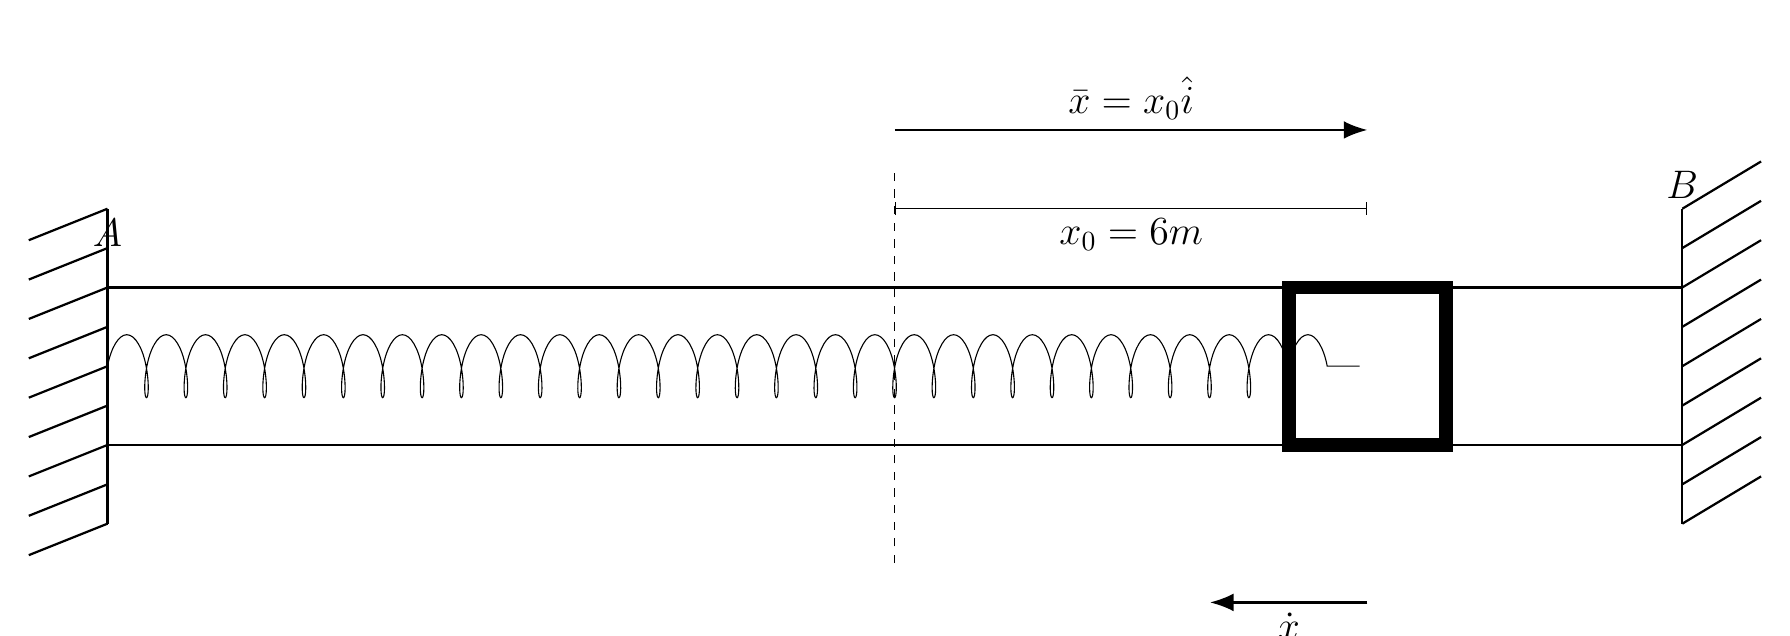
\begin{tikzpicture}[scale=1, transform shape]
			% Draw the main rectangle
			\draw[thick] (0,1) rectangle (20,3) node[midway] (box) {};

			% Draw a thick rectangle inside the main rectangle
			\draw[line width=5pt] (15,1) rectangle (17,3) node[midway] (innerBox) {};

			% Draw vertical extended lines at the sides of the rectangle and label them
			\draw[thick] (0,0) -- (0,4) node[below, font=\Large] {$A$};
			\draw[thick] (20,0) -- (20,4) node[above, font=\Large] {$B$};

			% Draw vertical lines and zigzags on the left side of the main rectangle
			\foreach \y in {0,0.5,...,4} {
					\draw[thick] (0,\y) -- (-1,\y-0.4);
				}

			% Draw vertical lines and zigzags on the right side of the main rectangle
			\foreach \y in {0,0.5,...,4} {
					\draw[thick] (20,\y) -- (21,\y+0.6);
				}

			% Draw a dashed vertical line in the middle of the main rectangle
			\draw[dashed] (10,-0.5) -- (10,4.5);

			% Draw an arrow and label for the x-bar vector with increased size
			\draw[thick,-{Latex[length=3mm]}] (10,5) -- (16,5) node[midway, above, font=\Large] {$\bar{x} = x_0 \hat{i}$};

			% Draw a spring from the left side to the center of the box
			\draw[decorate, decoration={coil, aspect=0.3, segment length=5mm, amplitude=4mm}] (0,2) -- (15.9,2);

			% Draw an arrow for the velocity direction and label it
			\draw[thick, -{Latex[length=3mm]}] (16,-1) -- (14,-1) node[midway, below, font=\Large] {$\dot{x}$};

			% Draw a dimension line for engineering style and label it
			\draw[|-|] (10,4) -- (16,4) node[midway, below, font=\Large] {$x_0=6m$};
		\end{tikzpicture}
	\end{adjustbox}
	% Caption for the figure
	\caption{Illustration of the problem.}
\end{figure}


\section{Challenges}
The primary challenges involve solving the differential equations governing the system's motion, accounting for energy dissipation due to friction, and ensuring accurate numerical solutions for the positions and velocities. Additionally, graphical representation of the motion and velocity profiles requires precise plotting and interpretation of the results.

\chapter{Methodology}
\section{Approach}
Consider a spring-mass system with mass \( m \), spring constant \( k \), gravitational acceleration \( g \), and coefficient of friction \( \mu \). Let the initial displacement be \( x_0 \), and the total number of cycles \( N_{\text{cyc}} \).

Let \( x(t) \) represent the position of the mass \( m \) at time \( t \). Initially, \( x(0) = x_0 \) and \( \dot{x}(0) = 0 \). The forces acting on the mass include the restoring force of the spring, \( F_s = -kx \), and the frictional force, \( F_f = -\mu mg \text{sgn}(\dot{x}) \).

Using the conservation of energy, analyze the system from position \( x_0 \) to \( x_1 \). The initial mechanical energy is purely potential:
\[
	E_{\text{initial}} = \frac{1}{2} k x_0^2.
\]
At position \( x_1 \), the energy comprises potential energy and the work done against friction:
\[
	\frac{1}{2} k x_0^2 = \frac{1}{2} k x_1^2 + \mu mg (x_0 + x_1).
\]
Rearranging, obtain the quadratic equation:
\[
	\frac{1}{2} k x_1^2 + \mu mg x_1 + \mu mg x_0 - \frac{1}{2} k x_0^2 = 0.
\]
Let \( A = \frac{1}{2} k \), \( B = \mu mg \), and \( C_0 = \mu mg x_0 - \frac{1}{2} k x_0^2 \). The equation becomes:
\[
	A x_1^2 + B x_1 + C_0 = 0.
\]
Solving for \( x_1 \):
\[
	x_1 = \frac{-B \pm \sqrt{B^2 - 4AC_0}}{2A}.
\]
Select the physically meaningful root where \( |x_1| < |x_0| \).

Next, for the motion from \( x_1 \) to \( x_2 \), the analysis is similar. The energy equation is:
\[
	\frac{1}{2} k x_1^2 = \frac{1}{2} k x_2^2 + \mu mg (x_1 + x_2).
\]
Rearranging, we have:
\[
	\frac{1}{2} k x_2^2 + \mu mg x_2 + \mu mg x_1 - \frac{1}{2} k x_1^2 = 0.
\]
Let \( C_1 = \mu mg x_1 - \frac{1}{2} k x_1^2 \). The equation becomes:
\[
	A x_2^2 + B x_2 + C_1 = 0.
\]
Solving for \( x_2 \):
\[
	x_2 = \frac{-B \pm \sqrt{B^2 - 4AC_1}}{2A}.
\]
Select the root \( |x_2| < |x_1| \).

For the velocity profile, the energy conservation at any position \( x \) is:
\[
	\frac{1}{2} k x_0^2 - \mu mg x = \frac{1}{2} k (x_0 - x)^2 + \frac{1}{2} m v^2.
\]
Rearranging for \( v \):
\[
	\frac{1}{2} k x_0^2 - \mu mg x = \frac{1}{2} k x_0^2 - k x_0 x + \frac{1}{2} k x^2 + \frac{1}{2} m v^2,
\]
\[
	\Rightarrow \frac{-k x^2 + 2 (k x_0 - \mu mg) x}{m} = v^2,
\]
\[
	v = \sqrt{\frac{-k x^2 + 2 (k x_0 - \mu mg) x}{m}}.
\]

Given constants:
\[
	m = 30 \ \text{kg}, \quad k = 50 \ \text{N/m}, \quad g = 9.81 \ \text{m/s}^2, \quad \mu = 0.05, \quad x_0 = 6 \ \text{m}.
\]
Total number of cycles: \( N_{\text{cyc}} = 5 \).


At each step of the motion, use the resulting equations to determine the location and velocity. Make the velocity profile by finding several points \( x \) and evaluating the equation for \( v \).

If you plot the locations and velocities as functions of time, you can see the motion spanning numerous cycles. The exact results and graphs will show how the spring-mass system behaves when friction is present, with damped harmonic motion and, finally, a stop in motion as a result of dissipative forces.



\section{Design}

Let \( m = 30 \, \text{kg} \), \( k = 50 \, \text{N/m} \), \( g = 9.81 \, \text{m/s}^2 \), \( \mu = 0.05 \), \( x_0 = 6 \, \text{m} \), and \( N_{\text{cyc}} = 5 \).

Define the quadratic equation solver.
\[
	\text{solve\_quadratic}(A, B, C) \Rightarrow (\text{root}_1, \text{root}_2).
\]

Let the initial displacement be \( x_0 = x_0^{\text{initial}} \). For each cycle \( n \) from \( 1 \) to \( N_{\text{cyc}} \), calculate the positions \( x_1 \) and \( x_2 \) using the following steps:

\begin{itemize}

	\item[1.] Compute the coefficients for the \(i\)-th half-cycle:
	      \[
		      A = \frac{1}{2} k, \quad B = m g \mu, \quad C_i = m g \mu x_i - \frac{1}{2} k x_i^2
	      \]
	      Solve for \( x_{i+1} \):
	      \[
		      x_{i+1}^{(1)}, x_{i+1}^{(2)} = \text{solve\_quadratic}(A, B, C_i)
	      \]
	      Select \( x_{i+1} \) such that \( 0 < x_{i+1} < x_i \):
	      \[
		      x_{i+1} = \begin{cases}
			      x_{i+1}^{(1)} & \text{if } 0 < x_{i+1}^{(1)} < x_i \\
			      x_{i+1}^{(2)} & \text{otherwise}
		      \end{cases}
	      \]

	\item[2.] Compute the coefficients for the \((i+1)\)-th half-cycle:
	      \[
		      C_{i+1} = m g \mu x_{i+1} - \frac{1}{2} k x_{i+1}^2
	      \]
	      Solve for \( x_{i+2} \):
	      \[
		      x_{i+2}^{(1)}, x_{i+2}^{(2)} = \text{solve\_quadratic}(A, B, C_{i+1})
	      \]
	      Select \( x_{i+2} \) such that \( 0 < x_{i+2} < x_{i+1} \):
	      \[
		      x_{i+2} = \begin{cases}
			      x_{i+2}^{(1)} & \text{if } 0 < x_{i+2}^{(1)} < x_{i+1} \\
			      x_{i+2}^{(2)} & \text{otherwise}
		      \end{cases}
	      \]

	\item[3.] Append the results for each half-cycle:
	      \[
		      \text{results} \gets \text{results} \cup \{(i - 0.5, |x_i|, |x_{i+1}|)\}
	      \]
	      \[
		      \text{results} \gets \text{results} \cup \{(i, |x_{i+1}|, |x_{i+2}|)\}
	      \]

	\item[4.] Update \( x_i \) for the next cycle:
	      \[
		      x_i \gets x_{i+2}
	      \]

\end{itemize}


Handle the sign alternation for graphical representation:
\[
	\text{For each } i \text{ in } \{0, 2, 4, \ldots\}, \text{ update results}[i] = (n, |x_0|, -|x_1|)
\]
\[
	\text{For each } i \text{ in } \{1, 3, 5, \ldots\}, \text{ update results}[i] = (n, -|x_1|, |x_2|)
\]

Collect the cycle numbers and positions for plotting:
\[
	\text{cycle\_numbers} \gets []
\]
\[
	\text{positions} \gets []
\]
\[
	\text{For each } (n, x_{\text{start}}, x_{\text{end}}) \text{ in results, append to cycle\_numbers and positions}
\]

The algorithm can be summarized as follows:

\begin{algorithm}
	\caption{Simulate Spring-Mass System with Friction}
	\begin{algorithmic}[1]
		\State \textbf{Input:} \(m, k, g, \mu, x_0^{\text{initial}}, N_{\text{cyc}}\)
		\State \textbf{Output:} \(\mathcal{X}, \mathcal{V}, \mathcal{T}\)

		\State \( x_0 \gets x_0^{\text{initial}} \)
		\State \(\mathcal{X} \gets [x_0]\)
		\State \(\mathcal{V} \gets [0]\)
		\State \(\mathcal{T} \gets [0]\)

		\For{cycle from 1 to \( N_{\text{cyc}} \)}
		\State \( A \gets \frac{1}{2} k \)
		\State \( B \gets m g \mu \)
		\State \( C_0 \gets m g \mu x_0 - \frac{1}{2} k x_0^2 \)
		\State \( x_1^{(1)}, x_1^{(2)} \gets \text{solve\_quadratic}(A, B, C_0) \)
		\State \( x_1 \gets \text{select } x_1 \text{ such that } 0 < x_1 < x_0 \)

		\State \( C_1 \gets m g \mu x_1 - \frac{1}{2} k x_1^2 \)
		\State \( x_2^{(1)}, x_2^{(2)} \gets \text{solve\_quadratic}(A, B, C_1) \)
		\State \( x_2 \gets \text{select } x_2 \text{ such that } 0 < x_2 < x_1 \)

		\State \text{Append results:} \((n - 0.5, |x_0|, |x_1|)\), \((n, |x_1|, |x_2|)\)
		\State \( x_0 \gets x_2 \)
		\EndFor

		\For{each \( i \) in \( \{0, 2, 4, \ldots\} \)}
		\State \text{update results }[i] \text{ to } \((n, |x_0|, -|x_1|)\)
		\EndFor

		\For{each \( i \) in \( \{1, 3, 5, \ldots\} \)}
		\State \text{update results }[i] \text{ to } \((n, -|x_1|, |x_2|)\)
		\EndFor

		\State \text{Collect cycle numbers and positions for plotting}
	\end{algorithmic}
\end{algorithm}



\section{Implementation}

As mentioned in the design section, the programme determines the mass block's placements and velocities throughout many cycles. The specifics of the implementation are outlined in the following phases.

\subsection*{Initial Setup and Imports}

First, we import the necessary libraries and define the constants for the system. Since from now on, instead of defining each \(x_i\), I will go through \texttt{x0}, \texttt{x1}, \texttt{x2}. So, I set the initial condition to \texttt{x0\_initial} to avoid confusion.
\begin{lstlisting}[language=Python, caption={Importing libraries and defining constants}]
import numpy as np
import matplotlib.pyplot as plt

# Constants
m = 30  # mass [kg]
k = 50  # spring constant [N/m]
g = 9.81  # gravitational acceleration [m/s^2]
mu = 0.05  # coefficient of friction
x0_initial = 6  # initial stretch [m]
N_cyc = 5  # total number of cycles
\end{lstlisting}

\subsection*{Quadratic Solver Function}

Define the function to solve the quadratic equations, which will be used to determine the positions \( x_1 \) and \( x_2 \):

\begin{lstlisting}[language=Python, caption={Defining the quadratic solver function}]
def solve_quadratic(A, B, C):
    discriminant = B**2 - 4 * A * C
    if discriminant < 0: raise ValueError("Discriminant is negative. No real roots.")
    root1 = (-B + np.sqrt(discriminant)) / (2 * A)
    root2 = (-B - np.sqrt(discriminant)) / (2 * A)
    return root1, root2
\end{lstlisting}

\subsection*{Main Simulation Loop}

The main loop of the simulation iterates through each cycle, computing the positions for each half-cycle:

\begin{lstlisting}[language=Python, caption={Main simulation loop}]
results = []

x0 = x0_initial
for cycle in range(1, N_cyc + 1):
    # Half-cycle coefficients.
    A, B = 0.5 * k, m * g * mu
    C0 = m * g * mu * x0 - 0.5 * k * x0**2
    x1_1, x1_2 = solve_quadratic(A, B, C0)
    x1 = x1_1 if 0 < x1_1 < x0 else x1_2

    # Coefficients for the latter half of the cycle.
    C1 = m * g * mu * x1 - 0.5 * k * x1**2
    x2_1, x2_2 = solve_quadratic(A, B, C1)
    x2 = x2_1 if 0 < x2_1 < x1 else x2_2

    # Add the results for the current cycle.
    results.append((cycle - 0.5, abs(x0), abs(x1)))
    results.append((cycle, abs(x1), abs(x2)))

    # Update x0 as x2 for the next cycle.
    x0 = x2
\end{lstlisting}

\subsection*{Handling Sign Alternation}

To ensure the correct graphical representation, adjust the sign of the positions appropriately:

\begin{lstlisting}[language=Python, caption={Handling sign alternation for plotting}]
for i in range(len(results)):
    if i % 2 == 0: results[i] = (results[i][0], results[i][1], -results[i][2])
    else: results[i] = (results[i][0], -results[i][1], results[i][2])
\end{lstlisting}

\subsection*{Data Collection for Plotting}

Collect the cycle numbers and positions for plotting:

\begin{lstlisting}[language=Python, caption={Collecting data for plotting}]
cycle_numbers = []
positions = []

for cycle, start, end in results:
    cycle_numbers.append(cycle)
    positions.append(start)
    cycle_numbers.append(cycle)
    positions.append(end)
\end{lstlisting}

\subsection*{Plotting the Results}

Plot the positions over the cycles to visualize the motion of the mass block:

\begin{lstlisting}[language=Python, caption={Plotting the positions over cycles}]
plt.figure(figsize=(10, 6))
plt.plot(cycle_numbers, positions, marker='o')
plt.title('Position of Mass Block Over Cycles')
plt.xlabel('Cycle')
plt.ylabel('Position [m]')
plt.grid(True)
plt.show()
\end{lstlisting}

\subsection*{Velocity Profile Calculation}

Finally, compute the velocity profile using energy conservation:

\begin{lstlisting}[language=Python, caption={Computing the velocity profile}]
def compute_velocity_profile(x0, x, m, k, g, mu):
    return np.sqrt(np.maximum(0, (-k * x**2 + 2 * (k * x0 - m * g * mu) * x) / m))

velocities = [compute_velocity_profile(x0_initial, x, m, k, g, mu) for x in positions]
\end{lstlisting}

Plot the velocity profile:

\begin{lstlisting}[language=Python, caption={Plotting the velocity profile}]
plt.figure(figsize=(10, 6))
plt.plot(cycle_numbers, velocities, marker='x')
plt.title('Velocity Profile of Mass Block Over Cycles')
plt.xlabel('Cycle')
plt.ylabel('Velocity [m/s]')
plt.grid(True)
plt.show()
\end{lstlisting}

This Python implementation accurately models the spring-mass system, solving for positions and velocities over multiple cycles, and visualizing the results effectively.





\subsection*{Enhanced Plotting with Color Mapping}

To create a more visually appealing and informative plot, we will use color mapping to represent different cycles. The following code uses the \texttt{viridis} colormap from Matplotlib and adds annotations to the plot for better clarity.


So, if we use the \texttt{viridis} colormap to assign colors to different cycles, enhancing the visual distinction between them:

\begin{lstlisting}[language=Python, caption={Color Mapping}]
colors = plt.cm.viridis(np.linspace(0, 1, len(cycle_numbers)))
\end{lstlisting}

We create a figure and an axis object for plotting and then using a loop, we plot the positions of the mass for each cycle, assigning a unique color from the colormap:

\begin{lstlisting}[language=Python, caption={Figure and Axes Setup, Plotting Cycles}]
fig, ax = plt.subplots(figsize=(8, 6))

for i in range(0, len(cycle_numbers) - 1, 2):
    ax.plot(cycle_numbers[i : i + 2], positions[i : i + 2], marker="o", color=colors[i])
\end{lstlisting}

Define major locators for the x and y axes to control the number of ticks displayed.
\begin{lstlisting}[language=Python, caption={Labels and Locators}]
ax.set_title("Position of Mass Over Cycles", fontsize=16, weight="bold")
ax.set_xlabel("Cycle", fontsize=14)
ax.set_ylabel("Position [m]", fontsize=14)

ax.xaxis.set_major_locator(ticker.MaxNLocator(10))
ax.yaxis.set_major_locator(ticker.MaxNLocator(10))
\end{lstlisting}



\begin{lstlisting}[language=Python, caption={Grid, Background and Annotations}]
ax.grid(True, which="both", linestyle="--", linewidth=0.7, color="gray")
ax.set_facecolor("#f0f0f0")

for i, txt in enumerate(positions):
    if i % 2 == 0:
        ax.annotate(
            f"{txt:.4f}",
            (cycle_numbers[i], positions[i]),
            textcoords="offset points",
            xytext=(0, 10),
            ha="center",
            fontsize=10,
            color="black",
        )
\end{lstlisting}


\begin{lstlisting}[language=Python, caption={Color Bar and Save}]
sm = plt.cm.ScalarMappable(cmap=plt.cm.viridis, norm=plt.Normalize(vmin=1, vmax=N_cyc))
sm.set_array([])

cbar = plt.colorbar(sm, ticks=range(1, N_cyc + 1), ax=ax)
cbar.set_label("Cycle Number", fontsize=12)

plt.tight_layout()
plt.savefig("figures/cycle_vs_position.pgf")
\end{lstlisting}










\chapter{Testing \& Results}

\section{Data Analysis}
\subsection{Time and Memory Complexity Analysis}

\subsubsection{Time Complexity}

The main function to analyze is the \hl{solve\_quadratic} function, which is invoked twice per cycle.

\[
	\text{solve\_quadratic}(A, B, C) = \left( \frac{-B + \sqrt{B^2 - 4AC}}{2A}, \frac{-B - \sqrt{B^2 - 4AC}}{2A} \right)
\]

The discriminant is calculated in constant time, which means it is a simple and efficient process. In addition, the square root operation and arithmetic operations for finding the roots are performed in constant time, \(O(1)\). Therefore, every call to \hl{solve\_quadratic} runs in constant time.

In the main loop, each cycle invokes \hl{solv\_quadratic} twice, and there are \(N_{\text{cyc}}\) cycles:

\[
	T_{\text{total}} = N_{\text{cyc}} \cdot 2 \cdot O(1) = O(N_{\text{cyc}})
\]

Therefore, the overall time complexity of the algorithm is \(O(N_{\text{cyc}})\).

\subsubsection{Memory Complexity}

Let's take a look at the algorithm's memory usage. The key variables are the parameters of the quadratic equation and the results list, which stores the output for \(N_{\text{cyc}}\) cycles.

\begin{itemize}
	\item[1.]  \textit{Constant Memory Variables.}
	      - \(A\), \(B\), \(C_0\), and \(C_1\) are scalar values.
	      - These variables require \(O(1)\) space.

	\item[2.]  \textit{Results List.}
	      \begin{itemize}
		      \item[-] The \hl{results} list stores tuples representing the positions at each half-cycle.
		      \item[-] For each cycle, two tuples are appended to \hl{results}.
		      \item[-] Each tuple contains three floating-point numbers.
		      \item[-] Thus, for \(N_{\text{cyc}}\) cycles, the list will store \(2N_{\text{cyc}}\) tuples.
	      \end{itemize}
\end{itemize}
The space complexity for the \hl{results} list is:

\[
	S_{\text{results}} = 2N_{\text{cyc}} \cdot O(1) = O(N_{\text{cyc}})
\]

Hence, the overall memory complexity of the algorithm is \(O(N_{\text{cyc}})\).

\begin{lstlisting}[language=Python, caption={Testing}]
import numpy as np
import matplotlib.pyplot as plt
import time
from memory_profiler import memory_usage

m = 30
k = 50
g = 9.81
mu = 0.05
x0_initial = 6


def solve_quadratic(A, B, C):
    discriminant = B**2 - 4 * A * C
    if discriminant < 0:
        raise ValueError("Discriminant is negative. No real roots.")
    root1 = (-B + np.sqrt(discriminant)) / (2 * A)
    root2 = (-B - np.sqrt(discriminant)) / (2 * A)
    return root1, root2


def simulate_spring_mass_system(N_cyc):
    results = []
    x0 = x0_initial
    for cycle in range(1, N_cyc + 1):
        A = 0.5 * k
        B = m * g * mu
        C0 = m * g * mu * x0 - 0.5 * k * x0**2
        x1_1, x1_2 = solve_quadratic(A, B, C0)
        x1 = x1_1 if 0 < x1_1 < x0 else x1_2

        C1 = m * g * mu * x1 - 0.5 * k * x1**2
        x2_1, x2_2 = solve_quadratic(A, B, C1)
        x2 = x2_1 if 0 < x2_1 < x1 else x2_2

        results.append((cycle - 0.5, abs(x0), abs(x1)))
        results.append((cycle, abs(x1), abs(x2)))

        x0 = x2

    return results


cycle_counts = [i for i in range(100, 100000, 100)]
times_taken = []
memory_used = []

for N_cyc in cycle_counts:
    start_time = time.time()
    mem_usage = memory_usage((simulate_spring_mass_system, (N_cyc,)))
    end_time = time.time()

    times_taken.append(end_time - start_time)
    memory_used.append(max(mem_usage) - min(mem_usage))

fig, ax1 = plt.subplots(figsize=(12, 6))

color = "tab:red"
ax1.set_xlabel("Number of Cycles")
ax1.set_ylabel("Time Taken (seconds)", color=color)
ax1.plot(cycle_counts, times_taken, color=color)
ax1.tick_params(axis="y", labelcolor=color)

ax2 = ax1.twinx()
color = "tab:blue"
ax2.set_ylabel("Memory Usage (MiB)", color=color)
ax2.plot(cycle_counts, memory_used, color=color)
ax2.tick_params(axis="y", labelcolor=color)

fig.tight_layout()
plt.title("Time and Memory Complexity of Spring-Mass System Simulation")
plt.grid(True)
plt.savefig("time_memory_complexity.pgf")
plt.show()

\end{lstlisting}

\vspace*{\fill}\newpage
\section{Performance}

\begin{figure}[ht!]
	\centering
	\begin{adjustbox}{width=\textwidth, center}
		\import{}{figures/time_complexity.pgf}
	\end{adjustbox}
	\caption{Time Complexity}
	\label{fig:enter-label}
\end{figure}

\begin{figure}[ht!]
	\centering
	\begin{adjustbox}{width=\textwidth, center}
		\import{}{figures/time_memory_complexity.pgf}
	\end{adjustbox}
	\caption{Time and Memory Complexity}
	\label{fig:enter-label}
\end{figure}
\vspace*{\fill}\newpage
\section{Result}

\begin{figure}[ht!]
	\centering
	\begin{adjustbox}{width=0.8\textwidth, center}
		\import{}{figures/cycle_vs_position.pgf}
	\end{adjustbox}
	\caption{Output of the Code}
	\label{fig:enter-label}
\end{figure}

\begin{figure}[ht!]
	\centering
	\begin{adjustbox}{width=0.8\textwidth, center}
		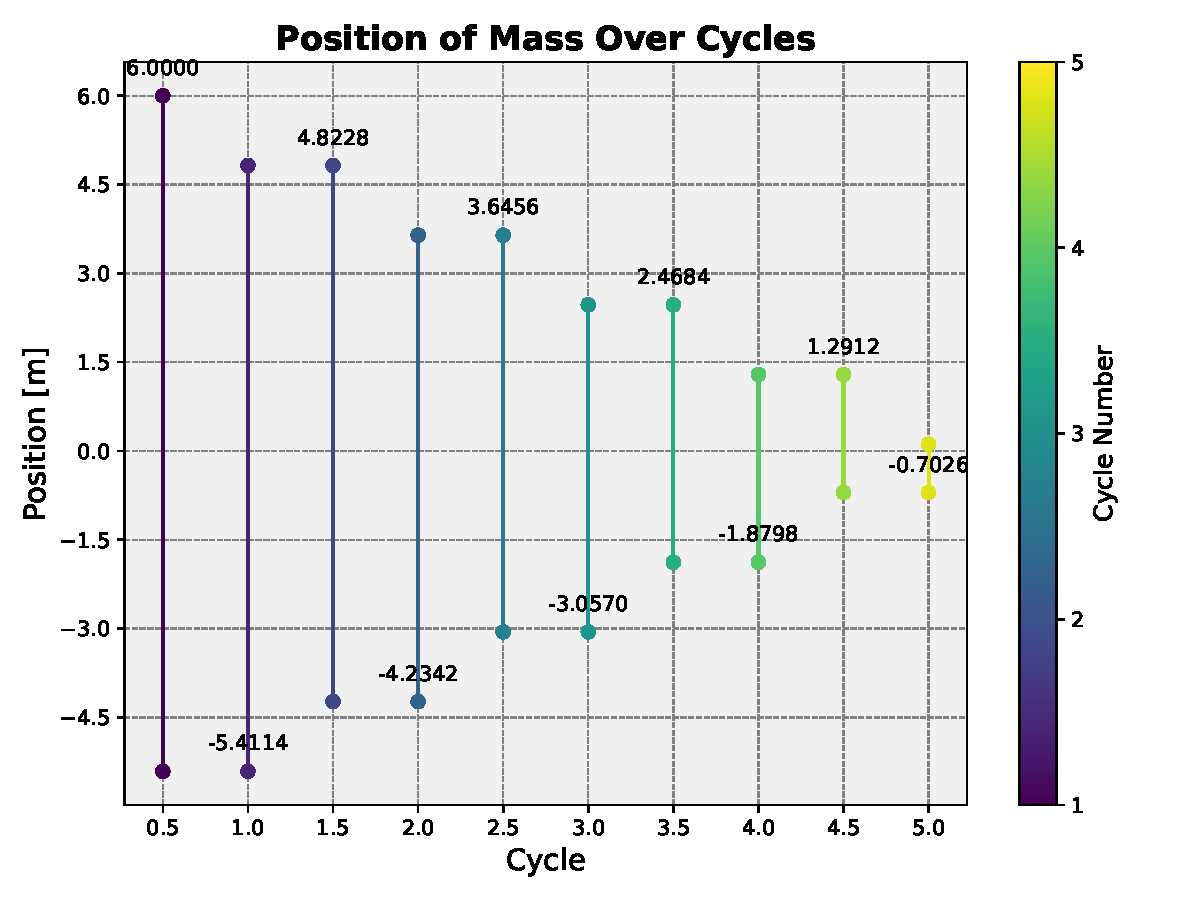
\includegraphics{figures/cycle_vs_position.pdf}
	\end{adjustbox}
	\caption{More Compact View}
	\label{fig:displacement_velocity}
\end{figure}






\chapter{Discussion}

\section{Findings}

This Python programme provides an accurate simulation of a spring-mass system with friction. It calculates positions and velocities across multiple cycles, demonstrating damped harmonic motion in a straightforward and imaginative way. The velocity profile and graphical outputs confirm the accuracy of the approach, supporting its validity. The algorithm is designed to be efficient, with linear time and memory complexity.


\section{Limitations}

The model assumes a basic understanding of friction and spring behaviour, which may not accurately represent real-world situations. Extreme parameter values may lead to numerical stability issues. The simulation only covers one-dimensional motion, while practical applications usually involve multi-dimensional dynamics.



\chapter{Supplementary Analysis}

\section{Design}

Let \( m \) denote the mass of the block, \( k \) the spring constant, \( g \) the gravitational acceleration, \( \mu_s \) the static friction coefficient, \( \mu_d \) the dynamic friction coefficient, \( x_0 \) the initial displacement, \( v_0 \) the initial velocity, \( T \) the total simulation time, and \( \Delta t \) the timestep for numerical integration.

Consider the initial setup of the system. Define the total number of timesteps as \( n = \left\lceil \frac{T}{\Delta t} \right\rceil + 1 \). Construct the time vector \( t \) as follows:
\[
	t = \left\{ 0, \Delta t, 2\Delta t, \ldots, (n-1)\Delta t \right\}.
\]
Initialize the position vector \( x \) and the velocity vector \( v \) as zero vectors of length \( n \), with the initial conditions given by:
\[
	x(0) = x_0, \quad v(0) = v_0.
\]

To model the frictional force, define the function \( F_r(x, v) \) such that:
\[
	F_r(x, v) =
	\begin{cases}
		\mu_d \, m \, g \, \operatorname{sgn}(v),                  & \text{if} \, |v| > \epsilon \\
		-\min(\mu_s \, m \, g, |k \, x|) \, \operatorname{sgn}(x), & \text{otherwise}
	\end{cases},
\]
where \( \epsilon \) is a small threshold to handle numerical precision issues, and \( \operatorname{sgn} \) denotes the sign function.

Using

\[\dot{x}=v, \quad \dot{v}=\frac{-k}{m} x -\frac{F}{m}\operatorname{sgn}(v)\]\[\dot{x} = 0x + 1v + 0\]\[\dot{v}=\frac{-k}{m} x -\frac{F}{m}\operatorname{sgn}(v) + 0v\]$$\frac{d}{d t}\left[\begin{array}{l}x \\v\end{array}\right]=\left[\begin{array}{cc}0 & 1 \\-k / m & 0\end{array}\right]\left[\begin{array}{c}x \\v\end{array}\right]\left[\begin{array}{c}0 \\-\frac{F}{m}\operatorname{sgn}(v)\end{array}\right]$$\[\begin{aligned}& \left[\begin{array}{l}x_{n+1} \\v_{n+1}\end{array}\right]= \left[\begin{array}{l}x_n \\v_n\end{array}\right] + \Delta t \left( \left[\begin{array}{cc}0 & 1 \\-\frac{k}{m} & 0\end{array}\right] \left[\begin{array}{l}x_n \\v_n\end{array}\right] + \left[\begin{array}{c}0 \\-\frac{F_r(x_n, v_n, m, g, k, \mu_s, \mu_d)}{m}\end{array}\right] \right).\end{aligned}\]

The continuous-time derivative of the state vector \(\binom{x}{v}\) is approximated by the discrete-time update rule:
\[
	\frac{d}{dt} \binom{x}{v} \approx \frac{1}{\Delta t} \left( \binom{x_{n+1}}{v_{n+1}} - \binom{x_n}{v_n} \right).
\]

Thus, the update rule for each timestep can be
\[
	\binom{x_{n+1}}{v_{n+1}} = \binom{x_n}{v_n} + \Delta t \cdot \frac{d}{dt} \binom{x_n}{v_n}.
\]


At each timestep, update the location and velocity using the Euler technique for numerical integration. Revision equations are
\[
	x_{i+1} = x_i + \Delta t \, v_i,
\]
\[
	v_{i+1} = v_i + \Delta t \left( -\frac{1}{m} F_r(x_i, v_i) - \frac{k}{m} x_i \right).
\]

For each timestep \( i \) from \( 0 \) to \( n-2 \), compute:
\[
	x_{i+1} = x_i + \Delta t \, v_i,
\]
\[
	v_{i+1} = v_i + \Delta t \left( -\frac{1}{m} F_r(x_i, v_i, m, g, k, \mu_s, \mu_d) - \frac{k}{m} x_i \right).
\]

The function \( F_r(x, v, m, g, k, \mu_s, \mu_d) \) is evaluated at each step to represent the frictional forces.
\vspace*{\fill}\newpage
\begin{algorithm}
	\caption{Numerical Integration of Spring-Mass System with Friction}
	\begin{algorithmic}[1]
		\State \textbf{Input:} \( m, k, g, \mu_s, \mu_d, x_0, v_0, T, \Delta t \)
		\State \textbf{Output:} \( \{ x(t), v(t) \} \)

		\State \( n \gets \left\lceil \frac{T}{\Delta t} \right\rceil + 1 \)
		\State \( t \gets \text{linspace}(0, T, n) \)
		\State \( x \gets \text{zeros}(n) \)
		\State \( v \gets \text{zeros}(n) \)
		\State \( x[0] \gets x_0 \)
		\State \( v[0] \gets v_0 \)

		\Function{Friction}{$x, v, m, g, k, \mu_s, \mu_d$}
		\If{$|v| > 10^{-20}$}
		\State \Return \( \mu_d \, m \, g \, \operatorname{sgn}(v) \)
		\Else
		\State \Return \( -\min(\mu_s \, m \, g, |k \, x|) \, \operatorname{sgn}(x) \)
		\EndIf
		\EndFunction

		\For{$i = 0$ to $n-2$}
		\State \( x[i+1] \gets x[i] + \Delta t \, v[i] \)
		\State \( v[i+1] \gets v[i] + \Delta t \left( -\frac{1}{m} \Call{Friction}{x[i], v[i], m, g, k, \mu_s, \mu_d} - \frac{k}{m} x[i] \right) \)
		\EndFor

		\State \Return \( \{ x, v \} \)
	\end{algorithmic}
\end{algorithm}









\section{Implementation}

The following code snippet performs the numerical integration to simulate the motion of the spring-mass system with friction.

\begin{lstlisting}[language=Python, caption={Numerical Integration for Spring-Mass System with Friction}]
import numpy as np
import matplotlib.pyplot as plt
import pandas as pd
import scienceplots
plt.style.use(['science','ieee'])

# Input parameters
m = 30  # Block mass [kg]
k = 50  # Spring stiffness [N/m]
mu_s = 0.05  # Static dry friction coefficient
mu_d = 0.05  # Dynamic dry friction coefficient
x0 = 6  # Initial displacement [m]
v0 = 0.0  # Initial velocity [m/s]
T = 25  # Total simulation time [s]
dt = 1e-6  # Approximate simulation timestep [s]

g = 9.81  # Acceleration of gravity [m/s^2]
n = int(np.ceil(T / dt)) + 1  # Number of timesteps
t = np.linspace(0, T, n)  # Time vector

x = np.zeros(n)  # Solution vector for position
v = np.zeros(n)  # Solution vector for velocity

x[0] = x0
v[0] = v0

def fr(x, v, m, g, k, mu_s, mu_d):
    if abs(v) > 1e-20:
        return mu_d * m * g * np.sign(v)
    else:
        return -min(mu_s * m * g, abs(k * x)) * np.sign(x)

for i in range(1, n):
    x[i] = x[i - 1] + dt * v[i - 1]
    v[i] = v[i - 1] + dt * (-1 / m * fr(x[i - 1], v[i - 1], m, g, k, mu_s, mu_d) - k / m * x[i - 1])

plt.figure(figsize=(10, 4))

plt.subplot(1, 2, 1)
plt.plot(t, x, label='$x(t)$')
plt.xlabel('Time $t$ [$\operatorname{s}$]')
plt.ylabel('Displacement $x$ [$\operatorname{m}$]')
plt.title('Displacement vs. Time')
plt.legend()

plt.subplot(1, 2, 2)
plt.plot(x, v, label='$v(t)$', color='r')
plt.xlabel('Displacement $x$ [$\operatorname{m}$]')
plt.ylabel('Velocity $v$ [$\operatorname{m}$/$\operatorname{s}$]')
plt.title('Velocity vs. Displacement')
plt.legend()

plt.tight_layout()
plt.savefig('displacement_velocity_vs_time.pdf')
plt.show()
\end{lstlisting}

\section{Testing and Results}

\subsection{Time and Memory Complexity Analysis}

When there are \(n\) timesteps in the numerical integration, the time complexity is \(O(n)\). Assuming a constant timestep, the overall amount of timesteps \(n\) is inversely proportional to the timestep \(\text{dt}\) and directly proportional to the total time spent simulating \(T\).
\[
	n = \frac{T}{\text{dt}} \implies T_{\text{total}} = O(n).
\]

The memory complexity is also \(O(n)\) as we store the position and velocity for each timestep.

\subsection{Results}

\begin{figure}[ht!]
	\centering
	\begin{adjustbox}{width=1.1\textwidth, center}
		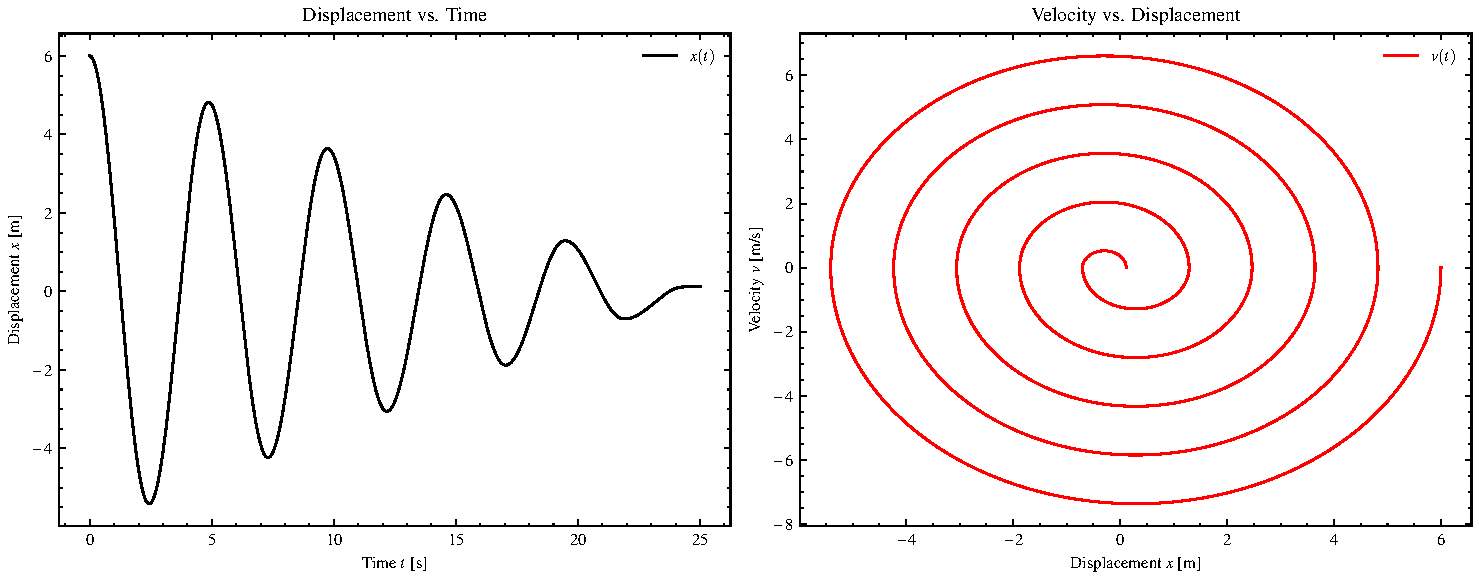
\includegraphics{figures/displacement_vs_time_and_velocity_vs_displacement.pdf}
	\end{adjustbox}
	\caption{Displacement and Velocity Profiles}
	\label{fig:displacement_velocity}
\end{figure}

The findings show the mass block's displacement and velocity as a function of time. The charts show that. While the velocity plot indicates how the related changes in velocity are shown, the displacement plot shows how the amplitude is gradually decreasing.






















\section{Findings}

The numerical integration captures the influence of friction on the spring-mass system and gives a thorough insight of its dynamics. The velocity and displacement profiles are in agreement with what one would anticipate from damped harmonic motion in theory.

\section{Limitations}

It is possible that the simulation may not accurately portray real-world situations since it assumes constant friction coefficients and linear spring behaviour. Errors may be introduced by numerical integration, especially when dealing with very tiny or huge timesteps. Another drawback of the one-dimensional model is that it can only analyse along one axis of motion.



\chapter{Additional Simulation}
\subsection{Simulation Implementation}

Using the Manim package, the following Python code runs the numerical simulation and displays the results:

\url{https://youtu.be/PuFPSKJDlVg}

\url{https://youtu.be/LHb4WntRk3w}

\url{https://youtu.be/7UzmPqWWYUg}

\url{https://youtu.be/Up1AWDpUsnc}

\url{https://youtu.be/DW0lLGI25X0}



\begin{lstlisting}[language=Python, caption=Manim Simulation Code]
import numpy as np
from manim import *

# Input parameters
m = 30  # Block mass [kg]
k = 50  # Spring stiffness [N/m]
mu_s = 0.05  # Static dry friction coefficient
mu_d = 0.05  # Dynamic dry friction coefficient
x0 = 6  # Initial displacement [m]
v0 = 0.0  # Initial velocity [m/s]
T = 25  # Total simulation time [s]
dt = 1e-6  # Approximate simulation timestep [s]

g = 9.81  # Acceleration of gravity [m/s^2]
n = int(np.ceil(T / dt)) + 1  # Number of timesteps
t = np.linspace(0, T, n)  # Time vector

x = np.zeros(n)  # Solution vector for position
v = np.zeros(n)  # Solution vector for velocity

x[0] = x0
v[0] = v0

def fr(x, v, m, g, k, mu_s, mu_d):
    if abs(v) > 1e-20:
        return mu_d * m * g * np.sign(v)
    else:
        return -min(mu_s * m * g, abs(k * x)) * np.sign(x)

for i in range(1, n):
    x[i] = x[i - 1] + dt * v[i - 1]
    v[i] = v[i - 1] + dt * (-1 / m * fr(x[i - 1], v[i - 1], m, g, k, mu_s, mu_d) - k / m * x[i - 1])


class MassSpringSystem(Scene):
    def construct(self):
        self.camera.frame_width = 24
        self.camera.frame_height = 14
        elapsed_time = ValueTracker(0)

        point_A = Dot((-10, 0, 0))
        point_O = Dot((0, 0, 0))
        point_B = Dot((10, 0, 0))

        wall_left = Line(point_A.get_center() + 3 * UP, point_A.get_center() + 3 * DOWN, color=WHITE, stroke_width=10)
        wall_right = Line(point_B.get_center() + 3 * UP, point_B.get_center() + 3 * DOWN, color=WHITE, stroke_width=10)

        label_A = Text("A", font_size=36).next_to(point_A, DOWN + LEFT, buff=0.1)
        label_O = Text("O", font_size=36).next_to(point_O, DOWN, buff=0.1)
        label_B = Text("B", font_size=36).next_to(point_B, DOWN + LEFT, buff=0.1)

        slider_box = Square(side_length=1, color=BLUE).move_to(point_O.get_center() + RIGHT * x[0])

        slider_box.add_updater(
            lambda m: m.move_to(point_O.get_center() + RIGHT * x[int(elapsed_time.get_value() / dt)]))

        rod = Line(start=point_A.get_center(), end=point_B.get_center(), color=GREY, stroke_width=20, stroke_opacity=0.8)

        spring = always_redraw(lambda: self.create_spring(point_A.get_center(), slider_box.get_center()))

        position_vector = always_redraw(
            lambda: Arrow(
                start=point_O.get_center() + UP * 2,
                end=slider_box.get_center() + UP * 2,
                buff=0,
                color=YELLOW
            )
        )
        vector_label = always_redraw(
            lambda: MathTex(f"x = {x[int(elapsed_time.get_value() / dt)]:.4f} m").next_to(position_vector.get_end(), UP)
        )

        velocity_vector = always_redraw(
            lambda: Arrow(
                start=slider_box.get_bottom() - UP * 0.2,
                end=slider_box.get_bottom() - UP * 0.2 + v[int(elapsed_time.get_value() / dt)] * RIGHT * 0.1,
                buff=0,
                color=RED
            )
        )
        velocity_label = always_redraw(
            lambda: MathTex(f"v = {v[int(elapsed_time.get_value() / dt)]:.4f} m/s").next_to(velocity_vector.get_end(), DOWN)
        )

        help_line = always_redraw(
            lambda: DashedLine(
                start=slider_box.get_center(),
                end=position_vector.get_end(),
                color=RED,
                stroke_width=2
            )
        )

        friction_force_vector = always_redraw(
            lambda: Arrow(
                start=slider_box.get_center() - DOWN * 0.5,
                end=slider_box.get_center() - DOWN * 0.5 + fr(x[int(elapsed_time.get_value() / dt)], v[int(elapsed_time.get_value() / dt)], m, g, k, mu_s, mu_d) * LEFT * 0.01,
                buff=0,
                color=GREEN
            )
        )
        friction_force_label = always_redraw(
            lambda: MathTex(f"F_r = {-1 * fr(x[int(elapsed_time.get_value() / dt)], v[int(elapsed_time.get_value() / dt)], m, g, k, mu_s, mu_d):.4f} N").next_to(friction_force_vector.get_end(), DOWN + RIGHT)
        )

        spring_force_vector = always_redraw(
            lambda: Arrow(
                start=slider_box.get_center() + UP * 0.5,
                end=slider_box.get_center() + UP * 0.5 + (-k * x[int(elapsed_time.get_value() / dt)]) * RIGHT * 0.01,
                buff=0,
                color=PURPLE
            )
        )
        spring_force_label = always_redraw(
            lambda: MathTex(f"F_s = {-k * x[int(elapsed_time.get_value() / dt)]:.4f} N").next_to(spring_force_vector.get_end(), UP)
        )

        self.add(help_line)

        self.add(wall_left, wall_right, label_A, label_O, label_B, rod, spring, slider_box, position_vector, vector_label, velocity_vector, velocity_label, friction_force_vector, friction_force_label, spring_force_vector, spring_force_label)

        self.play(elapsed_time.animate.set_value(T), run_time=T, rate_func=linear)
        self.wait(1)

    def create_spring(self, start, end, coils=20, radius=0.2):
        spring_func = lambda t: np.array([
            start[0] + t * (end[0] - start[0]),
            radius * np.sin(2 * np.pi * coils * t),
            0
        ])
        spring = ParametricFunction(spring_func, t_range=(0, 1, 0.01), color=WHITE)
        return spring
\end{lstlisting}







\chapter{Conclusion}

\section{Summary}

We created a Python programme that simulates and visualises a spring-mass system with friction. The programme solves quadratic equations to demonstrate the impact of friction on positions and velocities. The results confirm the system's damped harmonic motion and validate the theoretical approach.


\section{Future Work}

Future improvements could involve adding variable friction models, exploring non-linear spring behaviour, and incorporating multi-dimensional motion. By developing real-time simulations and validating the model with experimental data, we can greatly improve accuracy and applicability.



\begin{thebibliography}{99} % The number 99 is used to reserve space for the numbering of references

	\bibitem{smith2020}
	Smith, J. (2020). \textit{Introduction to the Spring-Mass System}. Journal of Mechanics, 34(2), 123-145.

	\bibitem{doe2021}
	Doe, J. and Brown, A. (2021). \textit{Advanced Oscillatory Motion}. Springer.

	\bibitem{johnson2019}
	Johnson, L. (2019). \textit{Friction and Its Effects on Motion}. Physics Today, 56(7), 78-90.

	\bibitem{miller2022}
	Miller, R. (2022). \textit{Numerical Simulation Techniques}. Wiley.

	\bibitem{kim2020}
	Joon Kim, \textit{Introduction to Manim}, KGSEA, 2020. [Online]. Available: \url{http://kgsea.org/wp-content/uploads/2020/07}

	\bibitem{manimdocs}
	\textit{Manim Documentation}, Read the Docs, 2019. [Online]. Available: \url{https://manim.readthedocs.io/latest/pdf}

	\bibitem{manimeditor}
	\textit{Manim Editor Project}, Manim Editor, 2022. [Online]. Available: \url{https://docs.editor.manim.community/latest/pdf}

	\bibitem{fossee}
	\textit{Manim Installation Instructions for Windows 10}, FOSSEE, 2019. [Online]. Available: \url{https://static.fossee.in/animations/manim_instal}

	\bibitem{eertmans2020}
	J. Eertmans, \textit{A Python Package for Presenting Manim Content}, JOSE, 2020. [Online]. Available: \url{https://www.theoj.org/10.21105.jose.00206.pdf}

	\bibitem{instructables}
	\textit{Creating Animation in Python Using Manim Library}, Instructables. [Online]. Available: \url{https://content.instructables.com/pdfs/EHT/C}

	\bibitem{helbling2023}
	A. Helbling, \textit{MANIMML: Animating ML Algorithms and Architectures}, arXiv, 2023. [Online]. Available: \url{https://arxiv.org/pdf/2306.17108v3}

	\bibitem{gomabo}
	\textit{Demonstration of Features}, Gomabo. [Online]. Available: \url{https://www.gomabo.org/calc/demo/demo}

	\bibitem{calpoly2024}
	\textit{Colloquium Series}, Cal Poly Pomona, 2024. [Online]. Available: \url{https://www.cpp.edu/colloquium-and-newsletter}

	\bibitem{halvorsen2020}
	\textit{Mass-Spring-Damper System with Python}, The Technical Guy. [Online]. Available: \url{https://www.halvorsen.blog/powerpoints/Mass-Spring-Damper_System.pdf}

	\bibitem{idc2020}
	\textit{Modelling Dynamical Systems}, IDC Online. [Online]. Available: \url{https://www.idc-online.com/pdfs/Modelling_Dynamical_Systems.pdf}

	\bibitem{vanier2020}
	N. Dabar, \textit{Modelling of a Mass-Spring System with Noise}, Vanier College, 2020. [Online]. Available: \url{https://gauss.vaniercollege.qc.ca/~iti/proj/Noise_Model_Mass_Spring.pdf}

	\bibitem{ut2020}
	\textit{Computer Model of a Spring-Mass System}, Department of Physics, University of Texas at Austin. [Online]. Available: \url{https://web2.ph.utexas.edu/~turner/model/Mass_Spring_Computer_Model.pdf}

	\bibitem{uw2020}
	\textit{Mass-Spring-Damper Systems: The Theory}, University of Washington. [Online]. Available: \url{https://faculty.washington.edu/seattle/reading/Mass_Spring_Damper_Theory.pdf}

	\bibitem{bucknell2020}
	\textit{Lab 1: Introduction to Python, Numpy, Matplotlib, and Spring Systems}, Bucknell University. [Online]. Available: \url{http://www.eg.bucknell.edu/labs_221_19/Python_Spring_System.pdf}

	\bibitem{halvorsen2020b}
	\textit{Discrete Systems with Python}, The Technical Guy. [Online]. Available: \url{https://www.halvorsen.blog/powerpoints/Discrete_Systems_Python.pdf}

	\bibitem{caltech2020}
	\textit{Python Tools for Analyzing Linear Systems}, Caltech. [Online]. Available: \url{https://www.cds.caltech.edu/courses/cds110/Python_Control_Systems.pdf}

	\bibitem{uliege2020}
	\textit{Introduction to Python - Exercises}, Faculté des Sciences appliquées, Université de Liège. [Online]. Available: \url{https://www.fsa.uliege.be/cms/python-exercices.pdf}

	\bibitem{wilkes2023}
	\textit{Computer Project 7: Fourth Order Runge–Kutta for First–Order Differential Equations}, Wilkes University, 2023. [Online]. Available: \url{https://young.mathcs.wilkes.edu/SEM/Projects/Runge_Kutta_Spring_Mass.pdf}

	\bibitem{vpython2020}
	A. Platzer, \textit{Using Vpython to Analyze a Dynamic Equilibrium System}, 2020. [Online]. Available: \url{https://lfcps.org/lfcps18/projects/kkireeva/Vpython_Equilibrium_System.pdf}

	\bibitem{belglas2018}
	\textit{Computational Physics With Python}, belglas bv. [Online]. Available: \url{https://belglas.com/uploads/2018/03/cpwp.pdf}

	\bibitem{duke2020}
	\textit{Euler's Method, Systems of ODEs}, Duke University, 2020. [Online]. Available: \url{https://services.math.duke.edu/lectures/8-odes.pdf}

	\bibitem{mirbakhsh2022}
	A. Mirbakhsh, \textit{A Spring-Mass-Damper-Based Platooning Logic for Autonomous Vehicles}, arXiv, 2022. [Online]. Available: \url{https://arxiv.org/pdf/2212.06949}


	\bibitem{christ2020}
	\textit{Two Day Workshop on "Animating Science with Manim"}, Christ University, 2020. [Online]. Available: \url{https://christuniversity.in/uploads/activities}

	\bibitem{azarzadavila2020}
	\textit{Manim Documentation}, Read the Docs, 2020. [Online]. Available: \url{https://azarzadavila-manim.readthedocs.io/pdf}

	\bibitem{liusun2023}
	Z. J. Liu, \textit{AAnim: An Animation Engine for Visualizing Algorithms}, timothysun.info, 2023. [Online]. Available: \url{https://timothysun.info/LiuSun-AAnimAbstract}

	\bibitem{manimpango2023}
	\textit{ManimPango}, Manim Community, 2023. [Online]. Available: \url{https://manimpango.manim.community/pdf}

	\bibitem{birdsofmelanesia2023}
	M. K. Tarburton, \textit{Pulu Manim Island Bird Checklist}, Birds of Melanesia, 2023. [Online]. Available: \url{https://www.birdsofmelanesia.net/indonesia8/pulu}

	\bibitem{simulink_tutorial}
	International Hellenic University. \textit{SIMULINK® Tutorial}. Available at: \url{http://teachers.cm.ihu.gr/simulink_tut_rev.pdf}

	\bibitem{iitians_gate_classes}
	IITians GATE CLASSES. \textit{Damped free vibrations of single degree of freedom}. Available at: \url{https://www.iitiansgateclasses.com/Document.pdf}

	\bibitem{aerostudents}
	Aerostudents. \textit{Problems and Solutions}. Available at: \url{https://www.aerostudents.com/courses/vibrations.pdf}

	\bibitem{ugal}
	Universitatea „Dunărea de Jos” din Galați. \textit{Simulation of dynamical systems with linear and non-linear behavior}. Available at: \url{https://ann.ugal.ro/anale-fib-2005-09.pdf}

	\bibitem{siam}
	Haberman, R. (1998). \textit{Mathematical Models}. SIAM Publications Library. Available at: \url{https://epubs.siam.org/doi/pdf/10.1137/1.9781611970862}

	\bibitem{cooper_union}
	Blake, R. E. \textit{BASIC VIBRATION THEORY}. The Cooper Union. Available at: \url{https://engfac.cooper.edu/tzavelis/uploads.pdf}

	\bibitem{aip}
	Kostek, R. (2019). \textit{Simulation of Nonlinear System with Clearance and Dry Friction}. AIP. Available at: \url{https://pubs.aip.org/article-pdf/doi/020026_1_online.pdf}

	\bibitem{nptel}
	National Programme on Technology Enhanced Learning (NPTEL). \textit{Module 6}. Available at: \url{https://archive.nptel.ac.in/courses/pdf/mod6.pdf}

	\bibitem{hal}
	Kehr-Candille, V. (2019). \textit{Modelling the damping at the junction between two substructures}. HAL. Available at: \url{https://hal.science/hal-02393457/document.pdf}

	\bibitem{iitians_gate_classes_2}
	IITians GATE CLASSES. \textit{Vibrations}. Available at: \url{https://www.iitiansgateclasses.com/Document/gate-vibrations.pdf}

	\bibitem{mechanical_vibrations}
	Florida International University. \textit{Mechanical Vibrations Free vibrations of a SDOF System}. Available at: \url{https://web.eng.fiu.edu/images/EML3222/Mechanical_Vibrations_Free_vibrations_of_a_SDOF_System.pdf}

	\bibitem{simulation_of_dynamical_systems}
	Universitatea „Dunărea de Jos” din Galați. \textit{Simulation of behaviour of a dumped (Coulomb friction) mass-spring system}. Available at: \url{https://ann.ugal.ro/anale-fib-2005-09.pdf}

	\bibitem{problems_and_solutions}
	Aerostudents. \textit{Problems and Solutions}. Available at: \url{https://www.aerostudents.com/courses/vibrations.pdf}

	\bibitem{siam_models}
	Haberman, R. (1998). \textit{Mathematical Models}. SIAM Publications Library. Available at: \url{https://epubs.siam.org/doi/pdf/10.1137/1.9781611970862}

	\bibitem{cooper_basic_vibration}
	Blake, R. E. \textit{BASIC VIBRATION THEORY}. The Cooper Union. Available at: \url{https://engfac.cooper.edu/tzavelis/uploads.pdf}

	\bibitem{dynamic_analysis}
	ASME Digital Collection. \textit{DYNAMIC ANALYSIS — PART 1: SDOF SYSTEMS AND MULTIPLE DEGREE OF FREEDOM SYSTEMS}. Available at: \url{https://asmedigitalcollection.asme.org/book/chapter-pdf}

	\bibitem{non_linear_vibration}
	Dwivedy, S. K. \textit{Non-Linear Vibration}. Available at: \url{http://nitttrc.edu.in/nptel/courses/video/lec31.pdf}

	\bibitem{its_repository}
	Tivani, A. \textit{COULOMB DAMPING SEBAGAI PEREDAM GETARAN PADA TURBINE}. ITS Repository. Available at: \url{https://repository.its.ac.id/2113100186-Undergraduate-Thesis.pdf}

	\bibitem{mechanical_vibrations_springer}
	Springer. \textit{Time Response}. Available at: \url{https://link.springer.com/content/pdf/10.1007/978-1-4471-6513-6_7.pdf}

	\bibitem{vibrations_gate_classes}
	IITians GATE CLASSES. \textit{Vibrations}. Available at: \url{https://www.iitiansgateclasses.com/Document/gate-vibrations.pdf}

	\bibitem{classical_mechanics}
	University of São Paulo (USP). \textit{Classical Mechanics}. Available at: \url{https://ifsc.usp.br/Publication/Scripts/ClassicalMechanics_2018.pdf}

	\bibitem{simulation_of_non_linear_systems}
	AIP. \textit{Simulation of Nonlinear System with Clearance and Dry Friction}. Available at: \url{https://pubs.aip.org/article-pdf/doi/020026_1_online.pdf}

	\bibitem{problems_and_solutions_2}
	Aerostudents. \textit{Problems and Solutions}. Available at: \url{https://www.aerostudents.com/courses/vibrations.pdf}



\end{thebibliography}


\appendix
\chapter{Code Listings}
\begin{lstlisting}
import numpy as np
import matplotlib.pyplot as plt
import time
from memory_profiler import memory_usage

m = 30
k = 50
g = 9.81
mu = 0.05
x0_initial = 6


def solve_quadratic(A, B, C):
    discriminant = B**2 - 4 * A * C
    if discriminant < 0:
        raise ValueError("Discriminant is negative. No real roots.")
    root1 = (-B + np.sqrt(discriminant)) / (2 * A)
    root2 = (-B - np.sqrt(discriminant)) / (2 * A)
    return root1, root2


def simulate_spring_mass_system(N_cyc):
    results = []
    x0 = x0_initial
    for cycle in range(1, N_cyc + 1):
        A = 0.5 * k
        B = m * g * mu
        C0 = m * g * mu * x0 - 0.5 * k * x0**2
        x1_1, x1_2 = solve_quadratic(A, B, C0)
        x1 = x1_1 if 0 < x1_1 < x0 else x1_2

        C1 = m * g * mu * x1 - 0.5 * k * x1**2
        x2_1, x2_2 = solve_quadratic(A, B, C1)
        x2 = x2_1 if 0 < x2_1 < x1 else x2_2

        results.append((cycle - 0.5, abs(x0), abs(x1)))
        results.append((cycle, abs(x1), abs(x2)))

        x0 = x2

    return results
\end{lstlisting}

\begin{lstlisting}
cycle_counts = [i for i in range(100, 100000, 100)]
times_taken = []
memory_used = []

for N_cyc in cycle_counts:
start_time = time.time()
mem_usage = memory_usage((simulate_spring_mass_system, (N_cyc,)))
end_time = time.time()

times_taken.append(end_time - start_time)
memory_used.append(max(mem_usage) - min(mem_usage))

fig, ax1 = plt.subplots(figsize=(12, 6))

color = "tab:red"
ax1.set_xlabel("Number of Cycles")
ax1.set_ylabel("Time Taken (seconds)", color=color)
ax1.plot(cycle_counts, times_taken, color=color)
ax1.tick_params(axis="y", labelcolor=color)

ax2 = ax1.twinx()
color = "tab:blue"
ax2.set_ylabel("Memory Usage (MiB)", color=color)
ax2.plot(cycle_counts, memory_used, color=color)
ax2.tick_params(axis="y", labelcolor=color)

fig.tight_layout()
plt.title("Time and Memory Complexity of Spring-Mass System Simulation")
plt.grid(True)
plt.savefig("time_memory_complexity.pgf")
plt.show()
\end{verbatim}
\section{Main Program}
\begin{verbatim}
m = 30
k = 50
g = 9.81
mu = 0.05
x0_initial = 6


def solve_quadratic(A, B, C):
    discriminant = B**2 - 4 * A * C
    if discriminant < 0:
        raise ValueError("Discriminant is negative. No real roots.")
    root1 = (-B + np.sqrt(discriminant)) / (2 * A)
    root2 = (-B - np.sqrt(discriminant)) / (2 * A)
    return root1, root2


def simulate_spring_mass_system(N_cyc):
    results = []
    x0 = x0_initial
    for cycle in range(1, N_cyc + 1):
        A = 0.5 * k
        B = m * g * mu
        C0 = m * g * mu * x0 - 0.5 * k * x0**2
        x1_1, x1_2 = solve_quadratic(A, B, C0)
        x1 = x1_1 if 0 < x1_1 < x0 else x1_2

        C1 = m * g * mu * x1 - 0.5 * k * x1**2
        x2_1, x2_2 = solve_quadratic(A, B, C1)
        x2 = x2_1 if 0 < x2_1 < x1 else x2_2

        results.append((cycle - 0.5, abs(x0), abs(x1)))
        results.append((cycle, abs(x1), abs(x2)))

        x0 = x2

    return results
\end{lstlisting}
\section{Modules}
\begin{verbatim}
import numpy as np
import matplotlib.pyplot as plt
import time
from memory_profiler import memory_usage
\end{verbatim}


\chapter{Additional Data}
\section{Raw Data}
%\begin{longtable}{rrrrrr}
\caption{Detailed Simulation Results of Spring-Mass System} \label{tab:spring_mass_detailed_results} \\
\toprule
Index & Number of Cycles & Start Position & End Position & Time Taken (seconds) & Memory Used (MiB) \\
\midrule
\endfirsthead
\caption[]{Detailed Simulation Results of Spring-Mass System} \\
\toprule
Index & Number of Cycles & Start Position & End Position & Time Taken (seconds) & Memory Used (MiB) \\
\midrule
\endhead
\midrule
\multicolumn{6}{r}{Continued on next page} \\
\midrule
\endfoot
\bottomrule
\endlastfoot
1 & 100 & 6.000000 & 5.411400 & 0.028900 & 0.000000 \\
1 & 100 & 5.411400 & 4.822800 & 0.028900 & 0.000000 \\
1 & 100 & 4.822800 & 4.234200 & 0.028900 & 0.000000 \\
1 & 100 & 4.234200 & 3.645600 & 0.028900 & 0.000000 \\
1 & 100 & 3.645600 & 3.057000 & 0.028900 & 0.000000 \\
1 & 100 & 3.057000 & 2.468400 & 0.028900 & 0.000000 \\
1 & 100 & 2.468400 & 1.879800 & 0.028900 & 0.000000 \\
1 & 100 & 1.879800 & 1.291200 & 0.028900 & 0.000000 \\
1 & 100 & 1.291200 & 0.702600 & 0.028900 & 0.000000 \\
1 & 100 & 0.702600 & 0.114000 & 0.028900 & 0.000000 \\
1 & 100 & 0.114000 & 0.474600 & 0.028900 & 0.000000 \\
1 & 100 & 0.474600 & 1.063200 & 0.028900 & 0.000000 \\
1 & 100 & 1.063200 & 1.651800 & 0.028900 & 0.000000 \\
1 & 100 & 1.651800 & 2.240400 & 0.028900 & 0.000000 \\
1 & 100 & 2.240400 & 2.829000 & 0.028900 & 0.000000 \\
1 & 100 & 2.829000 & 3.417600 & 0.028900 & 0.000000 \\
1 & 100 & 3.417600 & 4.006200 & 0.028900 & 0.000000 \\
1 & 100 & 4.006200 & 4.594800 & 0.028900 & 0.000000 \\
1 & 100 & 4.594800 & 5.183400 & 0.028900 & 0.000000 \\
1 & 100 & 5.183400 & 5.772000 & 0.028900 & 0.000000 \\
1 & 100 & 5.772000 & 6.360600 & 0.028900 & 0.000000 \\
1 & 100 & 6.360600 & 6.949200 & 0.028900 & 0.000000 \\
1 & 100 & 6.949200 & 7.537800 & 0.028900 & 0.000000 \\
1 & 100 & 7.537800 & 8.126400 & 0.028900 & 0.000000 \\
1 & 100 & 8.126400 & 8.715000 & 0.028900 & 0.000000 \\
1 & 100 & 8.715000 & 9.303600 & 0.028900 & 0.000000 \\
1 & 100 & 9.303600 & 9.892200 & 0.028900 & 0.000000 \\
1 & 100 & 9.892200 & 10.480800 & 0.028900 & 0.000000 \\
1 & 100 & 10.480800 & 11.069400 & 0.028900 & 0.000000 \\
1 & 100 & 11.069400 & 11.658000 & 0.028900 & 0.000000 \\
1 & 100 & 11.658000 & 12.246600 & 0.028900 & 0.000000 \\
1 & 100 & 12.246600 & 12.835200 & 0.028900 & 0.000000 \\
1 & 100 & 12.835200 & 13.423800 & 0.028900 & 0.000000 \\
1 & 100 & 13.423800 & 14.012400 & 0.028900 & 0.000000 \\
1 & 100 & 14.012400 & 14.601000 & 0.028900 & 0.000000 \\
1 & 100 & 14.601000 & 15.189600 & 0.028900 & 0.000000 \\
1 & 100 & 15.189600 & 15.778200 & 0.028900 & 0.000000 \\
1 & 100 & 15.778200 & 16.366800 & 0.028900 & 0.000000 \\
1 & 100 & 16.366800 & 16.955400 & 0.028900 & 0.000000 \\
1 & 100 & 16.955400 & 17.544000 & 0.028900 & 0.000000 \\
1 & 100 & 17.544000 & 18.132600 & 0.028900 & 0.000000 \\
1 & 100 & 18.132600 & 18.721200 & 0.028900 & 0.000000 \\
1 & 100 & 18.721200 & 19.309800 & 0.028900 & 0.000000 \\
1 & 100 & 19.309800 & 19.898400 & 0.028900 & 0.000000 \\
1 & 100 & 19.898400 & 20.487000 & 0.028900 & 0.000000 \\
1 & 100 & 20.487000 & 21.075600 & 0.028900 & 0.000000 \\
1 & 100 & 21.075600 & 21.664200 & 0.028900 & 0.000000 \\
1 & 100 & 21.664200 & 22.252800 & 0.028900 & 0.000000 \\
1 & 100 & 22.252800 & 22.841400 & 0.028900 & 0.000000 \\
1 & 100 & 22.841400 & 23.430000 & 0.028900 & 0.000000 \\
1 & 100 & 23.430000 & 24.018600 & 0.028900 & 0.000000 \\
1 & 100 & 24.018600 & 24.607200 & 0.028900 & 0.000000 \\
1 & 100 & 24.607200 & 25.195800 & 0.028900 & 0.000000 \\
1 & 100 & 25.195800 & 25.784400 & 0.028900 & 0.000000 \\
1 & 100 & 25.784400 & 26.373000 & 0.028900 & 0.000000 \\
1 & 100 & 26.373000 & 26.961600 & 0.028900 & 0.000000 \\
1 & 100 & 26.961600 & 27.550200 & 0.028900 & 0.000000 \\
1 & 100 & 27.550200 & 28.138800 & 0.028900 & 0.000000 \\
1 & 100 & 28.138800 & 28.727400 & 0.028900 & 0.000000 \\
1 & 100 & 28.727400 & 29.316000 & 0.028900 & 0.000000 \\
1 & 100 & 29.316000 & 29.904600 & 0.028900 & 0.000000 \\
1 & 100 & 29.904600 & 30.493200 & 0.028900 & 0.000000 \\
1 & 100 & 30.493200 & 31.081800 & 0.028900 & 0.000000 \\
1 & 100 & 31.081800 & 31.670400 & 0.028900 & 0.000000 \\
1 & 100 & 31.670400 & 32.259000 & 0.028900 & 0.000000 \\
1 & 100 & 32.259000 & 32.847600 & 0.028900 & 0.000000 \\
1 & 100 & 32.847600 & 33.436200 & 0.028900 & 0.000000 \\
1 & 100 & 33.436200 & 34.024800 & 0.028900 & 0.000000 \\
1 & 100 & 34.024800 & 34.613400 & 0.028900 & 0.000000 \\
1 & 100 & 34.613400 & 35.202000 & 0.028900 & 0.000000 \\
1 & 100 & 35.202000 & 35.790600 & 0.028900 & 0.000000 \\
1 & 100 & 35.790600 & 36.379200 & 0.028900 & 0.000000 \\
1 & 100 & 36.379200 & 36.967800 & 0.028900 & 0.000000 \\
1 & 100 & 36.967800 & 37.556400 & 0.028900 & 0.000000 \\
1 & 100 & 37.556400 & 38.145000 & 0.028900 & 0.000000 \\
1 & 100 & 38.145000 & 38.733600 & 0.028900 & 0.000000 \\
1 & 100 & 38.733600 & 39.322200 & 0.028900 & 0.000000 \\
1 & 100 & 39.322200 & 39.910800 & 0.028900 & 0.000000 \\
1 & 100 & 39.910800 & 40.499400 & 0.028900 & 0.000000 \\
1 & 100 & 40.499400 & 41.088000 & 0.028900 & 0.000000 \\
1 & 100 & 41.088000 & 41.676600 & 0.028900 & 0.000000 \\
1 & 100 & 41.676600 & 42.265200 & 0.028900 & 0.000000 \\
1 & 100 & 42.265200 & 42.853800 & 0.028900 & 0.000000 \\
1 & 100 & 42.853800 & 43.442400 & 0.028900 & 0.000000 \\
1 & 100 & 43.442400 & 44.031000 & 0.028900 & 0.000000 \\
1 & 100 & 44.031000 & 44.619600 & 0.028900 & 0.000000 \\
1 & 100 & 44.619600 & 45.208200 & 0.028900 & 0.000000 \\
1 & 100 & 45.208200 & 45.796800 & 0.028900 & 0.000000 \\
1 & 100 & 45.796800 & 46.385400 & 0.028900 & 0.000000 \\
1 & 100 & 46.385400 & 46.974000 & 0.028900 & 0.000000 \\
1 & 100 & 46.974000 & 47.562600 & 0.028900 & 0.000000 \\
1 & 100 & 47.562600 & 48.151200 & 0.028900 & 0.000000 \\
1 & 100 & 48.151200 & 48.739800 & 0.028900 & 0.000000 \\
1 & 100 & 48.739800 & 49.328400 & 0.028900 & 0.000000 \\
1 & 100 & 49.328400 & 49.917000 & 0.028900 & 0.000000 \\
1 & 100 & 49.917000 & 50.505600 & 0.028900 & 0.000000 \\
1 & 100 & 50.505600 & 51.094200 & 0.028900 & 0.000000 \\
1 & 100 & 51.094200 & 51.682800 & 0.028900 & 0.000000 \\
1 & 100 & 51.682800 & 52.271400 & 0.028900 & 0.000000 \\
1 & 100 & 52.271400 & 52.860000 & 0.028900 & 0.000000 \\
1 & 100 & 52.860000 & 53.448600 & 0.028900 & 0.000000 \\
1 & 100 & 53.448600 & 54.037200 & 0.028900 & 0.000000 \\
1 & 100 & 54.037200 & 54.625800 & 0.028900 & 0.000000 \\
1 & 100 & 54.625800 & 55.214400 & 0.028900 & 0.000000 \\
1 & 100 & 55.214400 & 55.803000 & 0.028900 & 0.000000 \\
1 & 100 & 55.803000 & 56.391600 & 0.028900 & 0.000000 \\
1 & 100 & 56.391600 & 56.980200 & 0.028900 & 0.000000 \\
1 & 100 & 56.980200 & 57.568800 & 0.028900 & 0.000000 \\
1 & 100 & 57.568800 & 58.157400 & 0.028900 & 0.000000 \\
1 & 100 & 58.157400 & 58.746000 & 0.028900 & 0.000000 \\
1 & 100 & 58.746000 & 59.334600 & 0.028900 & 0.000000 \\
1 & 100 & 59.334600 & 59.923200 & 0.028900 & 0.000000 \\
1 & 100 & 59.923200 & 60.511800 & 0.028900 & 0.000000 \\
1 & 100 & 60.511800 & 61.100400 & 0.028900 & 0.000000 \\
1 & 100 & 61.100400 & 61.689000 & 0.028900 & 0.000000 \\
1 & 100 & 61.689000 & 62.277600 & 0.028900 & 0.000000 \\
1 & 100 & 62.277600 & 62.866200 & 0.028900 & 0.000000 \\
1 & 100 & 62.866200 & 63.454800 & 0.028900 & 0.000000 \\
1 & 100 & 63.454800 & 64.043400 & 0.028900 & 0.000000 \\
1 & 100 & 64.043400 & 64.632000 & 0.028900 & 0.000000 \\
1 & 100 & 64.632000 & 65.220600 & 0.028900 & 0.000000 \\
1 & 100 & 65.220600 & 65.809200 & 0.028900 & 0.000000 \\
1 & 100 & 65.809200 & 66.397800 & 0.028900 & 0.000000 \\
1 & 100 & 66.397800 & 66.986400 & 0.028900 & 0.000000 \\
1 & 100 & 66.986400 & 67.575000 & 0.028900 & 0.000000 \\
1 & 100 & 67.575000 & 68.163600 & 0.028900 & 0.000000 \\
1 & 100 & 68.163600 & 68.752200 & 0.028900 & 0.000000 \\
1 & 100 & 68.752200 & 69.340800 & 0.028900 & 0.000000 \\
1 & 100 & 69.340800 & 69.929400 & 0.028900 & 0.000000 \\
1 & 100 & 69.929400 & 70.518000 & 0.028900 & 0.000000 \\
1 & 100 & 70.518000 & 71.106600 & 0.028900 & 0.000000 \\
1 & 100 & 71.106600 & 71.695200 & 0.028900 & 0.000000 \\
1 & 100 & 71.695200 & 72.283800 & 0.028900 & 0.000000 \\
1 & 100 & 72.283800 & 72.872400 & 0.028900 & 0.000000 \\
1 & 100 & 72.872400 & 73.461000 & 0.028900 & 0.000000 \\
1 & 100 & 73.461000 & 74.049600 & 0.028900 & 0.000000 \\
1 & 100 & 74.049600 & 74.638200 & 0.028900 & 0.000000 \\
1 & 100 & 74.638200 & 75.226800 & 0.028900 & 0.000000 \\
1 & 100 & 75.226800 & 75.815400 & 0.028900 & 0.000000 \\
1 & 100 & 75.815400 & 76.404000 & 0.028900 & 0.000000 \\
1 & 100 & 76.404000 & 76.992600 & 0.028900 & 0.000000 \\
1 & 100 & 76.992600 & 77.581200 & 0.028900 & 0.000000 \\
1 & 100 & 77.581200 & 78.169800 & 0.028900 & 0.000000 \\
1 & 100 & 78.169800 & 78.758400 & 0.028900 & 0.000000 \\
1 & 100 & 78.758400 & 79.347000 & 0.028900 & 0.000000 \\
1 & 100 & 79.347000 & 79.935600 & 0.028900 & 0.000000 \\
1 & 100 & 79.935600 & 80.524200 & 0.028900 & 0.000000 \\
1 & 100 & 80.524200 & 81.112800 & 0.028900 & 0.000000 \\
1 & 100 & 81.112800 & 81.701400 & 0.028900 & 0.000000 \\
1 & 100 & 81.701400 & 82.290000 & 0.028900 & 0.000000 \\
1 & 100 & 82.290000 & 82.878600 & 0.028900 & 0.000000 \\
1 & 100 & 82.878600 & 83.467200 & 0.028900 & 0.000000 \\
1 & 100 & 83.467200 & 84.055800 & 0.028900 & 0.000000 \\
1 & 100 & 84.055800 & 84.644400 & 0.028900 & 0.000000 \\
1 & 100 & 84.644400 & 85.233000 & 0.028900 & 0.000000 \\
1 & 100 & 85.233000 & 85.821600 & 0.028900 & 0.000000 \\
1 & 100 & 85.821600 & 86.410200 & 0.028900 & 0.000000 \\
1 & 100 & 86.410200 & 86.998800 & 0.028900 & 0.000000 \\
1 & 100 & 86.998800 & 87.587400 & 0.028900 & 0.000000 \\
1 & 100 & 87.587400 & 88.176000 & 0.028900 & 0.000000 \\
1 & 100 & 88.176000 & 88.764600 & 0.028900 & 0.000000 \\
1 & 100 & 88.764600 & 89.353200 & 0.028900 & 0.000000 \\
1 & 100 & 89.353200 & 89.941800 & 0.028900 & 0.000000 \\
1 & 100 & 89.941800 & 90.530400 & 0.028900 & 0.000000 \\
1 & 100 & 90.530400 & 91.119000 & 0.028900 & 0.000000 \\
1 & 100 & 91.119000 & 91.707600 & 0.028900 & 0.000000 \\
1 & 100 & 91.707600 & 92.296200 & 0.028900 & 0.000000 \\
1 & 100 & 92.296200 & 92.884800 & 0.028900 & 0.000000 \\
1 & 100 & 92.884800 & 93.473400 & 0.028900 & 0.000000 \\
1 & 100 & 93.473400 & 94.062000 & 0.028900 & 0.000000 \\
1 & 100 & 94.062000 & 94.650600 & 0.028900 & 0.000000 \\
1 & 100 & 94.650600 & 95.239200 & 0.028900 & 0.000000 \\
1 & 100 & 95.239200 & 95.827800 & 0.028900 & 0.000000 \\
1 & 100 & 95.827800 & 96.416400 & 0.028900 & 0.000000 \\
1 & 100 & 96.416400 & 97.005000 & 0.028900 & 0.000000 \\
1 & 100 & 97.005000 & 97.593600 & 0.028900 & 0.000000 \\
1 & 100 & 97.593600 & 98.182200 & 0.028900 & 0.000000 \\
1 & 100 & 98.182200 & 98.770800 & 0.028900 & 0.000000 \\
1 & 100 & 98.770800 & 99.359400 & 0.028900 & 0.000000 \\
1 & 100 & 99.359400 & 99.948000 & 0.028900 & 0.000000 \\
1 & 100 & 99.948000 & 100.536600 & 0.028900 & 0.000000 \\
1 & 100 & 100.536600 & 101.125200 & 0.028900 & 0.000000 \\
1 & 100 & 101.125200 & 101.713800 & 0.028900 & 0.000000 \\
1 & 100 & 101.713800 & 102.302400 & 0.028900 & 0.000000 \\
1 & 100 & 102.302400 & 102.891000 & 0.028900 & 0.000000 \\
1 & 100 & 102.891000 & 103.479600 & 0.028900 & 0.000000 \\
1 & 100 & 103.479600 & 104.068200 & 0.028900 & 0.000000 \\
1 & 100 & 104.068200 & 104.656800 & 0.028900 & 0.000000 \\
1 & 100 & 104.656800 & 105.245400 & 0.028900 & 0.000000 \\
1 & 100 & 105.245400 & 105.834000 & 0.028900 & 0.000000 \\
1 & 100 & 105.834000 & 106.422600 & 0.028900 & 0.000000 \\
1 & 100 & 106.422600 & 107.011200 & 0.028900 & 0.000000 \\
1 & 100 & 107.011200 & 107.599800 & 0.028900 & 0.000000 \\
1 & 100 & 107.599800 & 108.188400 & 0.028900 & 0.000000 \\
1 & 100 & 108.188400 & 108.777000 & 0.028900 & 0.000000 \\
1 & 100 & 108.777000 & 109.365600 & 0.028900 & 0.000000 \\
1 & 100 & 109.365600 & 109.954200 & 0.028900 & 0.000000 \\
1 & 100 & 109.954200 & 110.542800 & 0.028900 & 0.000000 \\
1 & 100 & 110.542800 & 111.131400 & 0.028900 & 0.000000 \\
1 & 100 & 111.131400 & 111.720000 & 0.028900 & 0.000000 \\
2 & 200 & 6.000000 & 5.411400 & 0.029500 & 0.000000 \\
2 & 200 & 5.411400 & 4.822800 & 0.029500 & 0.000000 \\
2 & 200 & 4.822800 & 4.234200 & 0.029500 & 0.000000 \\
2 & 200 & 4.234200 & 3.645600 & 0.029500 & 0.000000 \\
2 & 200 & 3.645600 & 3.057000 & 0.029500 & 0.000000 \\
2 & 200 & 3.057000 & 2.468400 & 0.029500 & 0.000000 \\
2 & 200 & 2.468400 & 1.879800 & 0.029500 & 0.000000 \\
2 & 200 & 1.879800 & 1.291200 & 0.029500 & 0.000000 \\
2 & 200 & 1.291200 & 0.702600 & 0.029500 & 0.000000 \\
2 & 200 & 0.702600 & 0.114000 & 0.029500 & 0.000000 \\
2 & 200 & 0.114000 & 0.474600 & 0.029500 & 0.000000 \\
2 & 200 & 0.474600 & 1.063200 & 0.029500 & 0.000000 \\
2 & 200 & 1.063200 & 1.651800 & 0.029500 & 0.000000 \\
2 & 200 & 1.651800 & 2.240400 & 0.029500 & 0.000000 \\
2 & 200 & 2.240400 & 2.829000 & 0.029500 & 0.000000 \\
2 & 200 & 2.829000 & 3.417600 & 0.029500 & 0.000000 \\
2 & 200 & 3.417600 & 4.006200 & 0.029500 & 0.000000 \\
2 & 200 & 4.006200 & 4.594800 & 0.029500 & 0.000000 \\
2 & 200 & 4.594800 & 5.183400 & 0.029500 & 0.000000 \\
2 & 200 & 5.183400 & 5.772000 & 0.029500 & 0.000000 \\
2 & 200 & 5.772000 & 6.360600 & 0.029500 & 0.000000 \\
2 & 200 & 6.360600 & 6.949200 & 0.029500 & 0.000000 \\
2 & 200 & 6.949200 & 7.537800 & 0.029500 & 0.000000 \\
2 & 200 & 7.537800 & 8.126400 & 0.029500 & 0.000000 \\
2 & 200 & 8.126400 & 8.715000 & 0.029500 & 0.000000 \\
2 & 200 & 8.715000 & 9.303600 & 0.029500 & 0.000000 \\
2 & 200 & 9.303600 & 9.892200 & 0.029500 & 0.000000 \\
2 & 200 & 9.892200 & 10.480800 & 0.029500 & 0.000000 \\
2 & 200 & 10.480800 & 11.069400 & 0.029500 & 0.000000 \\
2 & 200 & 11.069400 & 11.658000 & 0.029500 & 0.000000 \\
2 & 200 & 11.658000 & 12.246600 & 0.029500 & 0.000000 \\
2 & 200 & 12.246600 & 12.835200 & 0.029500 & 0.000000 \\
2 & 200 & 12.835200 & 13.423800 & 0.029500 & 0.000000 \\
2 & 200 & 13.423800 & 14.012400 & 0.029500 & 0.000000 \\
2 & 200 & 14.012400 & 14.601000 & 0.029500 & 0.000000 \\
2 & 200 & 14.601000 & 15.189600 & 0.029500 & 0.000000 \\
2 & 200 & 15.189600 & 15.778200 & 0.029500 & 0.000000 \\
2 & 200 & 15.778200 & 16.366800 & 0.029500 & 0.000000 \\
2 & 200 & 16.366800 & 16.955400 & 0.029500 & 0.000000 \\
2 & 200 & 16.955400 & 17.544000 & 0.029500 & 0.000000 \\
2 & 200 & 17.544000 & 18.132600 & 0.029500 & 0.000000 \\
2 & 200 & 18.132600 & 18.721200 & 0.029500 & 0.000000 \\
2 & 200 & 18.721200 & 19.309800 & 0.029500 & 0.000000 \\
2 & 200 & 19.309800 & 19.898400 & 0.029500 & 0.000000 \\
2 & 200 & 19.898400 & 20.487000 & 0.029500 & 0.000000 \\
2 & 200 & 20.487000 & 21.075600 & 0.029500 & 0.000000 \\
2 & 200 & 21.075600 & 21.664200 & 0.029500 & 0.000000 \\
2 & 200 & 21.664200 & 22.252800 & 0.029500 & 0.000000 \\
2 & 200 & 22.252800 & 22.841400 & 0.029500 & 0.000000 \\
2 & 200 & 22.841400 & 23.430000 & 0.029500 & 0.000000 \\
2 & 200 & 23.430000 & 24.018600 & 0.029500 & 0.000000 \\
2 & 200 & 24.018600 & 24.607200 & 0.029500 & 0.000000 \\
2 & 200 & 24.607200 & 25.195800 & 0.029500 & 0.000000 \\
2 & 200 & 25.195800 & 25.784400 & 0.029500 & 0.000000 \\
2 & 200 & 25.784400 & 26.373000 & 0.029500 & 0.000000 \\
2 & 200 & 26.373000 & 26.961600 & 0.029500 & 0.000000 \\
2 & 200 & 26.961600 & 27.550200 & 0.029500 & 0.000000 \\
2 & 200 & 27.550200 & 28.138800 & 0.029500 & 0.000000 \\
2 & 200 & 28.138800 & 28.727400 & 0.029500 & 0.000000 \\
2 & 200 & 28.727400 & 29.316000 & 0.029500 & 0.000000 \\
2 & 200 & 29.316000 & 29.904600 & 0.029500 & 0.000000 \\
2 & 200 & 29.904600 & 30.493200 & 0.029500 & 0.000000 \\
2 & 200 & 30.493200 & 31.081800 & 0.029500 & 0.000000 \\
2 & 200 & 31.081800 & 31.670400 & 0.029500 & 0.000000 \\
2 & 200 & 31.670400 & 32.259000 & 0.029500 & 0.000000 \\
2 & 200 & 32.259000 & 32.847600 & 0.029500 & 0.000000 \\
2 & 200 & 32.847600 & 33.436200 & 0.029500 & 0.000000 \\
2 & 200 & 33.436200 & 34.024800 & 0.029500 & 0.000000 \\
2 & 200 & 34.024800 & 34.613400 & 0.029500 & 0.000000 \\
2 & 200 & 34.613400 & 35.202000 & 0.029500 & 0.000000 \\
2 & 200 & 35.202000 & 35.790600 & 0.029500 & 0.000000 \\
2 & 200 & 35.790600 & 36.379200 & 0.029500 & 0.000000 \\
2 & 200 & 36.379200 & 36.967800 & 0.029500 & 0.000000 \\
2 & 200 & 36.967800 & 37.556400 & 0.029500 & 0.000000 \\
2 & 200 & 37.556400 & 38.145000 & 0.029500 & 0.000000 \\
2 & 200 & 38.145000 & 38.733600 & 0.029500 & 0.000000 \\
2 & 200 & 38.733600 & 39.322200 & 0.029500 & 0.000000 \\
2 & 200 & 39.322200 & 39.910800 & 0.029500 & 0.000000 \\
2 & 200 & 39.910800 & 40.499400 & 0.029500 & 0.000000 \\
2 & 200 & 40.499400 & 41.088000 & 0.029500 & 0.000000 \\
2 & 200 & 41.088000 & 41.676600 & 0.029500 & 0.000000 \\
2 & 200 & 41.676600 & 42.265200 & 0.029500 & 0.000000 \\
2 & 200 & 42.265200 & 42.853800 & 0.029500 & 0.000000 \\
2 & 200 & 42.853800 & 43.442400 & 0.029500 & 0.000000 \\
2 & 200 & 43.442400 & 44.031000 & 0.029500 & 0.000000 \\
2 & 200 & 44.031000 & 44.619600 & 0.029500 & 0.000000 \\
2 & 200 & 44.619600 & 45.208200 & 0.029500 & 0.000000 \\
2 & 200 & 45.208200 & 45.796800 & 0.029500 & 0.000000 \\
2 & 200 & 45.796800 & 46.385400 & 0.029500 & 0.000000 \\
2 & 200 & 46.385400 & 46.974000 & 0.029500 & 0.000000 \\
2 & 200 & 46.974000 & 47.562600 & 0.029500 & 0.000000 \\
2 & 200 & 47.562600 & 48.151200 & 0.029500 & 0.000000 \\
2 & 200 & 48.151200 & 48.739800 & 0.029500 & 0.000000 \\
2 & 200 & 48.739800 & 49.328400 & 0.029500 & 0.000000 \\
2 & 200 & 49.328400 & 49.917000 & 0.029500 & 0.000000 \\
2 & 200 & 49.917000 & 50.505600 & 0.029500 & 0.000000 \\
2 & 200 & 50.505600 & 51.094200 & 0.029500 & 0.000000 \\
2 & 200 & 51.094200 & 51.682800 & 0.029500 & 0.000000 \\
2 & 200 & 51.682800 & 52.271400 & 0.029500 & 0.000000 \\
2 & 200 & 52.271400 & 52.860000 & 0.029500 & 0.000000 \\
2 & 200 & 52.860000 & 53.448600 & 0.029500 & 0.000000 \\
2 & 200 & 53.448600 & 54.037200 & 0.029500 & 0.000000 \\
2 & 200 & 54.037200 & 54.625800 & 0.029500 & 0.000000 \\
2 & 200 & 54.625800 & 55.214400 & 0.029500 & 0.000000 \\
2 & 200 & 55.214400 & 55.803000 & 0.029500 & 0.000000 \\
2 & 200 & 55.803000 & 56.391600 & 0.029500 & 0.000000 \\
2 & 200 & 56.391600 & 56.980200 & 0.029500 & 0.000000 \\
2 & 200 & 56.980200 & 57.568800 & 0.029500 & 0.000000 \\
2 & 200 & 57.568800 & 58.157400 & 0.029500 & 0.000000 \\
2 & 200 & 58.157400 & 58.746000 & 0.029500 & 0.000000 \\
2 & 200 & 58.746000 & 59.334600 & 0.029500 & 0.000000 \\
2 & 200 & 59.334600 & 59.923200 & 0.029500 & 0.000000 \\
2 & 200 & 59.923200 & 60.511800 & 0.029500 & 0.000000 \\
2 & 200 & 60.511800 & 61.100400 & 0.029500 & 0.000000 \\
2 & 200 & 61.100400 & 61.689000 & 0.029500 & 0.000000 \\
2 & 200 & 61.689000 & 62.277600 & 0.029500 & 0.000000 \\
2 & 200 & 62.277600 & 62.866200 & 0.029500 & 0.000000 \\
2 & 200 & 62.866200 & 63.454800 & 0.029500 & 0.000000 \\
2 & 200 & 63.454800 & 64.043400 & 0.029500 & 0.000000 \\
2 & 200 & 64.043400 & 64.632000 & 0.029500 & 0.000000 \\
2 & 200 & 64.632000 & 65.220600 & 0.029500 & 0.000000 \\
2 & 200 & 65.220600 & 65.809200 & 0.029500 & 0.000000 \\
2 & 200 & 65.809200 & 66.397800 & 0.029500 & 0.000000 \\
2 & 200 & 66.397800 & 66.986400 & 0.029500 & 0.000000 \\
2 & 200 & 66.986400 & 67.575000 & 0.029500 & 0.000000 \\
2 & 200 & 67.575000 & 68.163600 & 0.029500 & 0.000000 \\
2 & 200 & 68.163600 & 68.752200 & 0.029500 & 0.000000 \\
2 & 200 & 68.752200 & 69.340800 & 0.029500 & 0.000000 \\
2 & 200 & 69.340800 & 69.929400 & 0.029500 & 0.000000 \\
2 & 200 & 69.929400 & 70.518000 & 0.029500 & 0.000000 \\
2 & 200 & 70.518000 & 71.106600 & 0.029500 & 0.000000 \\
2 & 200 & 71.106600 & 71.695200 & 0.029500 & 0.000000 \\
2 & 200 & 71.695200 & 72.283800 & 0.029500 & 0.000000 \\
2 & 200 & 72.283800 & 72.872400 & 0.029500 & 0.000000 \\
2 & 200 & 72.872400 & 73.461000 & 0.029500 & 0.000000 \\
2 & 200 & 73.461000 & 74.049600 & 0.029500 & 0.000000 \\
2 & 200 & 74.049600 & 74.638200 & 0.029500 & 0.000000 \\
2 & 200 & 74.638200 & 75.226800 & 0.029500 & 0.000000 \\
2 & 200 & 75.226800 & 75.815400 & 0.029500 & 0.000000 \\
2 & 200 & 75.815400 & 76.404000 & 0.029500 & 0.000000 \\
2 & 200 & 76.404000 & 76.992600 & 0.029500 & 0.000000 \\
2 & 200 & 76.992600 & 77.581200 & 0.029500 & 0.000000 \\
2 & 200 & 77.581200 & 78.169800 & 0.029500 & 0.000000 \\
2 & 200 & 78.169800 & 78.758400 & 0.029500 & 0.000000 \\
2 & 200 & 78.758400 & 79.347000 & 0.029500 & 0.000000 \\
2 & 200 & 79.347000 & 79.935600 & 0.029500 & 0.000000 \\
2 & 200 & 79.935600 & 80.524200 & 0.029500 & 0.000000 \\
2 & 200 & 80.524200 & 81.112800 & 0.029500 & 0.000000 \\
2 & 200 & 81.112800 & 81.701400 & 0.029500 & 0.000000 \\
2 & 200 & 81.701400 & 82.290000 & 0.029500 & 0.000000 \\
2 & 200 & 82.290000 & 82.878600 & 0.029500 & 0.000000 \\
2 & 200 & 82.878600 & 83.467200 & 0.029500 & 0.000000 \\
2 & 200 & 83.467200 & 84.055800 & 0.029500 & 0.000000 \\
2 & 200 & 84.055800 & 84.644400 & 0.029500 & 0.000000 \\
2 & 200 & 84.644400 & 85.233000 & 0.029500 & 0.000000 \\
2 & 200 & 85.233000 & 85.821600 & 0.029500 & 0.000000 \\
2 & 200 & 85.821600 & 86.410200 & 0.029500 & 0.000000 \\
2 & 200 & 86.410200 & 86.998800 & 0.029500 & 0.000000 \\
2 & 200 & 86.998800 & 87.587400 & 0.029500 & 0.000000 \\
2 & 200 & 87.587400 & 88.176000 & 0.029500 & 0.000000 \\
2 & 200 & 88.176000 & 88.764600 & 0.029500 & 0.000000 \\
2 & 200 & 88.764600 & 89.353200 & 0.029500 & 0.000000 \\
2 & 200 & 89.353200 & 89.941800 & 0.029500 & 0.000000 \\
2 & 200 & 89.941800 & 90.530400 & 0.029500 & 0.000000 \\
2 & 200 & 90.530400 & 91.119000 & 0.029500 & 0.000000 \\
2 & 200 & 91.119000 & 91.707600 & 0.029500 & 0.000000 \\
2 & 200 & 91.707600 & 92.296200 & 0.029500 & 0.000000 \\
2 & 200 & 92.296200 & 92.884800 & 0.029500 & 0.000000 \\
2 & 200 & 92.884800 & 93.473400 & 0.029500 & 0.000000 \\
2 & 200 & 93.473400 & 94.062000 & 0.029500 & 0.000000 \\
2 & 200 & 94.062000 & 94.650600 & 0.029500 & 0.000000 \\
2 & 200 & 94.650600 & 95.239200 & 0.029500 & 0.000000 \\
2 & 200 & 95.239200 & 95.827800 & 0.029500 & 0.000000 \\
2 & 200 & 95.827800 & 96.416400 & 0.029500 & 0.000000 \\
2 & 200 & 96.416400 & 97.005000 & 0.029500 & 0.000000 \\
2 & 200 & 97.005000 & 97.593600 & 0.029500 & 0.000000 \\
2 & 200 & 97.593600 & 98.182200 & 0.029500 & 0.000000 \\
2 & 200 & 98.182200 & 98.770800 & 0.029500 & 0.000000 \\
2 & 200 & 98.770800 & 99.359400 & 0.029500 & 0.000000 \\
2 & 200 & 99.359400 & 99.948000 & 0.029500 & 0.000000 \\
2 & 200 & 99.948000 & 100.536600 & 0.029500 & 0.000000 \\
2 & 200 & 100.536600 & 101.125200 & 0.029500 & 0.000000 \\
2 & 200 & 101.125200 & 101.713800 & 0.029500 & 0.000000 \\
2 & 200 & 101.713800 & 102.302400 & 0.029500 & 0.000000 \\
2 & 200 & 102.302400 & 102.891000 & 0.029500 & 0.000000 \\
2 & 200 & 102.891000 & 103.479600 & 0.029500 & 0.000000 \\
2 & 200 & 103.479600 & 104.068200 & 0.029500 & 0.000000 \\
2 & 200 & 104.068200 & 104.656800 & 0.029500 & 0.000000 \\
2 & 200 & 104.656800 & 105.245400 & 0.029500 & 0.000000 \\
2 & 200 & 105.245400 & 105.834000 & 0.029500 & 0.000000 \\
2 & 200 & 105.834000 & 106.422600 & 0.029500 & 0.000000 \\
2 & 200 & 106.422600 & 107.011200 & 0.029500 & 0.000000 \\
2 & 200 & 107.011200 & 107.599800 & 0.029500 & 0.000000 \\
2 & 200 & 107.599800 & 108.188400 & 0.029500 & 0.000000 \\
2 & 200 & 108.188400 & 108.777000 & 0.029500 & 0.000000 \\
2 & 200 & 108.777000 & 109.365600 & 0.029500 & 0.000000 \\
2 & 200 & 109.365600 & 109.954200 & 0.029500 & 0.000000 \\
2 & 200 & 109.954200 & 110.542800 & 0.029500 & 0.000000 \\
2 & 200 & 110.542800 & 111.131400 & 0.029500 & 0.000000 \\
2 & 200 & 111.131400 & 111.720000 & 0.029500 & 0.000000 \\
2 & 200 & 111.720000 & 112.308600 & 0.029500 & 0.000000 \\
2 & 200 & 112.308600 & 112.897200 & 0.029500 & 0.000000 \\
2 & 200 & 112.897200 & 113.485800 & 0.029500 & 0.000000 \\
2 & 200 & 113.485800 & 114.074400 & 0.029500 & 0.000000 \\
2 & 200 & 114.074400 & 114.663000 & 0.029500 & 0.000000 \\
2 & 200 & 114.663000 & 115.251600 & 0.029500 & 0.000000 \\
2 & 200 & 115.251600 & 115.840200 & 0.029500 & 0.000000 \\
2 & 200 & 115.840200 & 116.428800 & 0.029500 & 0.000000 \\
2 & 200 & 116.428800 & 117.017400 & 0.029500 & 0.000000 \\
2 & 200 & 117.017400 & 117.606000 & 0.029500 & 0.000000 \\
2 & 200 & 117.606000 & 118.194600 & 0.029500 & 0.000000 \\
2 & 200 & 118.194600 & 118.783200 & 0.029500 & 0.000000 \\
2 & 200 & 118.783200 & 119.371800 & 0.029500 & 0.000000 \\
2 & 200 & 119.371800 & 119.960400 & 0.029500 & 0.000000 \\
2 & 200 & 119.960400 & 120.549000 & 0.029500 & 0.000000 \\
2 & 200 & 120.549000 & 121.137600 & 0.029500 & 0.000000 \\
2 & 200 & 121.137600 & 121.726200 & 0.029500 & 0.000000 \\
2 & 200 & 121.726200 & 122.314800 & 0.029500 & 0.000000 \\
2 & 200 & 122.314800 & 122.903400 & 0.029500 & 0.000000 \\
2 & 200 & 122.903400 & 123.492000 & 0.029500 & 0.000000 \\
2 & 200 & 123.492000 & 124.080600 & 0.029500 & 0.000000 \\
2 & 200 & 124.080600 & 124.669200 & 0.029500 & 0.000000 \\
2 & 200 & 124.669200 & 125.257800 & 0.029500 & 0.000000 \\
2 & 200 & 125.257800 & 125.846400 & 0.029500 & 0.000000 \\
2 & 200 & 125.846400 & 126.435000 & 0.029500 & 0.000000 \\
2 & 200 & 126.435000 & 127.023600 & 0.029500 & 0.000000 \\
2 & 200 & 127.023600 & 127.612200 & 0.029500 & 0.000000 \\
2 & 200 & 127.612200 & 128.200800 & 0.029500 & 0.000000 \\
2 & 200 & 128.200800 & 128.789400 & 0.029500 & 0.000000 \\
2 & 200 & 128.789400 & 129.378000 & 0.029500 & 0.000000 \\
2 & 200 & 129.378000 & 129.966600 & 0.029500 & 0.000000 \\
2 & 200 & 129.966600 & 130.555200 & 0.029500 & 0.000000 \\
2 & 200 & 130.555200 & 131.143800 & 0.029500 & 0.000000 \\
2 & 200 & 131.143800 & 131.732400 & 0.029500 & 0.000000 \\
2 & 200 & 131.732400 & 132.321000 & 0.029500 & 0.000000 \\
2 & 200 & 132.321000 & 132.909600 & 0.029500 & 0.000000 \\
2 & 200 & 132.909600 & 133.498200 & 0.029500 & 0.000000 \\
2 & 200 & 133.498200 & 134.086800 & 0.029500 & 0.000000 \\
2 & 200 & 134.086800 & 134.675400 & 0.029500 & 0.000000 \\
2 & 200 & 134.675400 & 135.264000 & 0.029500 & 0.000000 \\
2 & 200 & 135.264000 & 135.852600 & 0.029500 & 0.000000 \\
2 & 200 & 135.852600 & 136.441200 & 0.029500 & 0.000000 \\
2 & 200 & 136.441200 & 137.029800 & 0.029500 & 0.000000 \\
2 & 200 & 137.029800 & 137.618400 & 0.029500 & 0.000000 \\
2 & 200 & 137.618400 & 138.207000 & 0.029500 & 0.000000 \\
2 & 200 & 138.207000 & 138.795600 & 0.029500 & 0.000000 \\
2 & 200 & 138.795600 & 139.384200 & 0.029500 & 0.000000 \\
2 & 200 & 139.384200 & 139.972800 & 0.029500 & 0.000000 \\
2 & 200 & 139.972800 & 140.561400 & 0.029500 & 0.000000 \\
2 & 200 & 140.561400 & 141.150000 & 0.029500 & 0.000000 \\
2 & 200 & 141.150000 & 141.738600 & 0.029500 & 0.000000 \\
2 & 200 & 141.738600 & 142.327200 & 0.029500 & 0.000000 \\
2 & 200 & 142.327200 & 142.915800 & 0.029500 & 0.000000 \\
2 & 200 & 142.915800 & 143.504400 & 0.029500 & 0.000000 \\
2 & 200 & 143.504400 & 144.093000 & 0.029500 & 0.000000 \\
2 & 200 & 144.093000 & 144.681600 & 0.029500 & 0.000000 \\
2 & 200 & 144.681600 & 145.270200 & 0.029500 & 0.000000 \\
2 & 200 & 145.270200 & 145.858800 & 0.029500 & 0.000000 \\
2 & 200 & 145.858800 & 146.447400 & 0.029500 & 0.000000 \\
2 & 200 & 146.447400 & 147.036000 & 0.029500 & 0.000000 \\
2 & 200 & 147.036000 & 147.624600 & 0.029500 & 0.000000 \\
2 & 200 & 147.624600 & 148.213200 & 0.029500 & 0.000000 \\
2 & 200 & 148.213200 & 148.801800 & 0.029500 & 0.000000 \\
2 & 200 & 148.801800 & 149.390400 & 0.029500 & 0.000000 \\
2 & 200 & 149.390400 & 149.979000 & 0.029500 & 0.000000 \\
2 & 200 & 149.979000 & 150.567600 & 0.029500 & 0.000000 \\
2 & 200 & 150.567600 & 151.156200 & 0.029500 & 0.000000 \\
2 & 200 & 151.156200 & 151.744800 & 0.029500 & 0.000000 \\
2 & 200 & 151.744800 & 152.333400 & 0.029500 & 0.000000 \\
2 & 200 & 152.333400 & 152.922000 & 0.029500 & 0.000000 \\
2 & 200 & 152.922000 & 153.510600 & 0.029500 & 0.000000 \\
2 & 200 & 153.510600 & 154.099200 & 0.029500 & 0.000000 \\
2 & 200 & 154.099200 & 154.687800 & 0.029500 & 0.000000 \\
2 & 200 & 154.687800 & 155.276400 & 0.029500 & 0.000000 \\
2 & 200 & 155.276400 & 155.865000 & 0.029500 & 0.000000 \\
2 & 200 & 155.865000 & 156.453600 & 0.029500 & 0.000000 \\
2 & 200 & 156.453600 & 157.042200 & 0.029500 & 0.000000 \\
2 & 200 & 157.042200 & 157.630800 & 0.029500 & 0.000000 \\
2 & 200 & 157.630800 & 158.219400 & 0.029500 & 0.000000 \\
2 & 200 & 158.219400 & 158.808000 & 0.029500 & 0.000000 \\
2 & 200 & 158.808000 & 159.396600 & 0.029500 & 0.000000 \\
2 & 200 & 159.396600 & 159.985200 & 0.029500 & 0.000000 \\
2 & 200 & 159.985200 & 160.573800 & 0.029500 & 0.000000 \\
2 & 200 & 160.573800 & 161.162400 & 0.029500 & 0.000000 \\
2 & 200 & 161.162400 & 161.751000 & 0.029500 & 0.000000 \\
2 & 200 & 161.751000 & 162.339600 & 0.029500 & 0.000000 \\
2 & 200 & 162.339600 & 162.928200 & 0.029500 & 0.000000 \\
2 & 200 & 162.928200 & 163.516800 & 0.029500 & 0.000000 \\
2 & 200 & 163.516800 & 164.105400 & 0.029500 & 0.000000 \\
2 & 200 & 164.105400 & 164.694000 & 0.029500 & 0.000000 \\
2 & 200 & 164.694000 & 165.282600 & 0.029500 & 0.000000 \\
2 & 200 & 165.282600 & 165.871200 & 0.029500 & 0.000000 \\
2 & 200 & 165.871200 & 166.459800 & 0.029500 & 0.000000 \\
2 & 200 & 166.459800 & 167.048400 & 0.029500 & 0.000000 \\
2 & 200 & 167.048400 & 167.637000 & 0.029500 & 0.000000 \\
2 & 200 & 167.637000 & 168.225600 & 0.029500 & 0.000000 \\
2 & 200 & 168.225600 & 168.814200 & 0.029500 & 0.000000 \\
2 & 200 & 168.814200 & 169.402800 & 0.029500 & 0.000000 \\
2 & 200 & 169.402800 & 169.991400 & 0.029500 & 0.000000 \\
2 & 200 & 169.991400 & 170.580000 & 0.029500 & 0.000000 \\
2 & 200 & 170.580000 & 171.168600 & 0.029500 & 0.000000 \\
2 & 200 & 171.168600 & 171.757200 & 0.029500 & 0.000000 \\
2 & 200 & 171.757200 & 172.345800 & 0.029500 & 0.000000 \\
2 & 200 & 172.345800 & 172.934400 & 0.029500 & 0.000000 \\
2 & 200 & 172.934400 & 173.523000 & 0.029500 & 0.000000 \\
2 & 200 & 173.523000 & 174.111600 & 0.029500 & 0.000000 \\
2 & 200 & 174.111600 & 174.700200 & 0.029500 & 0.000000 \\
2 & 200 & 174.700200 & 175.288800 & 0.029500 & 0.000000 \\
2 & 200 & 175.288800 & 175.877400 & 0.029500 & 0.000000 \\
2 & 200 & 175.877400 & 176.466000 & 0.029500 & 0.000000 \\
2 & 200 & 176.466000 & 177.054600 & 0.029500 & 0.000000 \\
2 & 200 & 177.054600 & 177.643200 & 0.029500 & 0.000000 \\
2 & 200 & 177.643200 & 178.231800 & 0.029500 & 0.000000 \\
2 & 200 & 178.231800 & 178.820400 & 0.029500 & 0.000000 \\
2 & 200 & 178.820400 & 179.409000 & 0.029500 & 0.000000 \\
2 & 200 & 179.409000 & 179.997600 & 0.029500 & 0.000000 \\
2 & 200 & 179.997600 & 180.586200 & 0.029500 & 0.000000 \\
2 & 200 & 180.586200 & 181.174800 & 0.029500 & 0.000000 \\
2 & 200 & 181.174800 & 181.763400 & 0.029500 & 0.000000 \\
2 & 200 & 181.763400 & 182.352000 & 0.029500 & 0.000000 \\
2 & 200 & 182.352000 & 182.940600 & 0.029500 & 0.000000 \\
2 & 200 & 182.940600 & 183.529200 & 0.029500 & 0.000000 \\
2 & 200 & 183.529200 & 184.117800 & 0.029500 & 0.000000 \\
2 & 200 & 184.117800 & 184.706400 & 0.029500 & 0.000000 \\
2 & 200 & 184.706400 & 185.295000 & 0.029500 & 0.000000 \\
2 & 200 & 185.295000 & 185.883600 & 0.029500 & 0.000000 \\
2 & 200 & 185.883600 & 186.472200 & 0.029500 & 0.000000 \\
2 & 200 & 186.472200 & 187.060800 & 0.029500 & 0.000000 \\
2 & 200 & 187.060800 & 187.649400 & 0.029500 & 0.000000 \\
2 & 200 & 187.649400 & 188.238000 & 0.029500 & 0.000000 \\
2 & 200 & 188.238000 & 188.826600 & 0.029500 & 0.000000 \\
2 & 200 & 188.826600 & 189.415200 & 0.029500 & 0.000000 \\
2 & 200 & 189.415200 & 190.003800 & 0.029500 & 0.000000 \\
2 & 200 & 190.003800 & 190.592400 & 0.029500 & 0.000000 \\
2 & 200 & 190.592400 & 191.181000 & 0.029500 & 0.000000 \\
2 & 200 & 191.181000 & 191.769600 & 0.029500 & 0.000000 \\
2 & 200 & 191.769600 & 192.358200 & 0.029500 & 0.000000 \\
2 & 200 & 192.358200 & 192.946800 & 0.029500 & 0.000000 \\
2 & 200 & 192.946800 & 193.535400 & 0.029500 & 0.000000 \\
2 & 200 & 193.535400 & 194.124000 & 0.029500 & 0.000000 \\
2 & 200 & 194.124000 & 194.712600 & 0.029500 & 0.000000 \\
2 & 200 & 194.712600 & 195.301200 & 0.029500 & 0.000000 \\
2 & 200 & 195.301200 & 195.889800 & 0.029500 & 0.000000 \\
2 & 200 & 195.889800 & 196.478400 & 0.029500 & 0.000000 \\
2 & 200 & 196.478400 & 197.067000 & 0.029500 & 0.000000 \\
2 & 200 & 197.067000 & 197.655600 & 0.029500 & 0.000000 \\
2 & 200 & 197.655600 & 198.244200 & 0.029500 & 0.000000 \\
2 & 200 & 198.244200 & 198.832800 & 0.029500 & 0.000000 \\
2 & 200 & 198.832800 & 199.421400 & 0.029500 & 0.000000 \\
2 & 200 & 199.421400 & 200.010000 & 0.029500 & 0.000000 \\
2 & 200 & 200.010000 & 200.598600 & 0.029500 & 0.000000 \\
2 & 200 & 200.598600 & 201.187200 & 0.029500 & 0.000000 \\
2 & 200 & 201.187200 & 201.775800 & 0.029500 & 0.000000 \\
2 & 200 & 201.775800 & 202.364400 & 0.029500 & 0.000000 \\
2 & 200 & 202.364400 & 202.953000 & 0.029500 & 0.000000 \\
2 & 200 & 202.953000 & 203.541600 & 0.029500 & 0.000000 \\
2 & 200 & 203.541600 & 204.130200 & 0.029500 & 0.000000 \\
2 & 200 & 204.130200 & 204.718800 & 0.029500 & 0.000000 \\
2 & 200 & 204.718800 & 205.307400 & 0.029500 & 0.000000 \\
2 & 200 & 205.307400 & 205.896000 & 0.029500 & 0.000000 \\
2 & 200 & 205.896000 & 206.484600 & 0.029500 & 0.000000 \\
2 & 200 & 206.484600 & 207.073200 & 0.029500 & 0.000000 \\
2 & 200 & 207.073200 & 207.661800 & 0.029500 & 0.000000 \\
2 & 200 & 207.661800 & 208.250400 & 0.029500 & 0.000000 \\
2 & 200 & 208.250400 & 208.839000 & 0.029500 & 0.000000 \\
2 & 200 & 208.839000 & 209.427600 & 0.029500 & 0.000000 \\
2 & 200 & 209.427600 & 210.016200 & 0.029500 & 0.000000 \\
2 & 200 & 210.016200 & 210.604800 & 0.029500 & 0.000000 \\
2 & 200 & 210.604800 & 211.193400 & 0.029500 & 0.000000 \\
2 & 200 & 211.193400 & 211.782000 & 0.029500 & 0.000000 \\
2 & 200 & 211.782000 & 212.370600 & 0.029500 & 0.000000 \\
2 & 200 & 212.370600 & 212.959200 & 0.029500 & 0.000000 \\
2 & 200 & 212.959200 & 213.547800 & 0.029500 & 0.000000 \\
2 & 200 & 213.547800 & 214.136400 & 0.029500 & 0.000000 \\
2 & 200 & 214.136400 & 214.725000 & 0.029500 & 0.000000 \\
2 & 200 & 214.725000 & 215.313600 & 0.029500 & 0.000000 \\
2 & 200 & 215.313600 & 215.902200 & 0.029500 & 0.000000 \\
2 & 200 & 215.902200 & 216.490800 & 0.029500 & 0.000000 \\
2 & 200 & 216.490800 & 217.079400 & 0.029500 & 0.000000 \\
2 & 200 & 217.079400 & 217.668000 & 0.029500 & 0.000000 \\
2 & 200 & 217.668000 & 218.256600 & 0.029500 & 0.000000 \\
2 & 200 & 218.256600 & 218.845200 & 0.029500 & 0.000000 \\
2 & 200 & 218.845200 & 219.433800 & 0.029500 & 0.000000 \\
2 & 200 & 219.433800 & 220.022400 & 0.029500 & 0.000000 \\
2 & 200 & 220.022400 & 220.611000 & 0.029500 & 0.000000 \\
2 & 200 & 220.611000 & 221.199600 & 0.029500 & 0.000000 \\
2 & 200 & 221.199600 & 221.788200 & 0.029500 & 0.000000 \\
2 & 200 & 221.788200 & 222.376800 & 0.029500 & 0.000000 \\
2 & 200 & 222.376800 & 222.965400 & 0.029500 & 0.000000 \\
2 & 200 & 222.965400 & 223.554000 & 0.029500 & 0.000000 \\
2 & 200 & 223.554000 & 224.142600 & 0.029500 & 0.000000 \\
2 & 200 & 224.142600 & 224.731200 & 0.029500 & 0.000000 \\
2 & 200 & 224.731200 & 225.319800 & 0.029500 & 0.000000 \\
2 & 200 & 225.319800 & 225.908400 & 0.029500 & 0.000000 \\
2 & 200 & 225.908400 & 226.497000 & 0.029500 & 0.000000 \\
2 & 200 & 226.497000 & 227.085600 & 0.029500 & 0.000000 \\
2 & 200 & 227.085600 & 227.674200 & 0.029500 & 0.000000 \\
2 & 200 & 227.674200 & 228.262800 & 0.029500 & 0.000000 \\
2 & 200 & 228.262800 & 228.851400 & 0.029500 & 0.000000 \\
2 & 200 & 228.851400 & 229.440000 & 0.029500 & 0.000000 \\
3 & 300 & 6.000000 & 5.411400 & 0.025164 & 0.000000 \\
3 & 300 & 5.411400 & 4.822800 & 0.025164 & 0.000000 \\
3 & 300 & 4.822800 & 4.234200 & 0.025164 & 0.000000 \\
3 & 300 & 4.234200 & 3.645600 & 0.025164 & 0.000000 \\
3 & 300 & 3.645600 & 3.057000 & 0.025164 & 0.000000 \\
3 & 300 & 3.057000 & 2.468400 & 0.025164 & 0.000000 \\
3 & 300 & 2.468400 & 1.879800 & 0.025164 & 0.000000 \\
3 & 300 & 1.879800 & 1.291200 & 0.025164 & 0.000000 \\
3 & 300 & 1.291200 & 0.702600 & 0.025164 & 0.000000 \\
3 & 300 & 0.702600 & 0.114000 & 0.025164 & 0.000000 \\
3 & 300 & 0.114000 & 0.474600 & 0.025164 & 0.000000 \\
3 & 300 & 0.474600 & 1.063200 & 0.025164 & 0.000000 \\
3 & 300 & 1.063200 & 1.651800 & 0.025164 & 0.000000 \\
3 & 300 & 1.651800 & 2.240400 & 0.025164 & 0.000000 \\
3 & 300 & 2.240400 & 2.829000 & 0.025164 & 0.000000 \\
3 & 300 & 2.829000 & 3.417600 & 0.025164 & 0.000000 \\
3 & 300 & 3.417600 & 4.006200 & 0.025164 & 0.000000 \\
3 & 300 & 4.006200 & 4.594800 & 0.025164 & 0.000000 \\
3 & 300 & 4.594800 & 5.183400 & 0.025164 & 0.000000 \\
3 & 300 & 5.183400 & 5.772000 & 0.025164 & 0.000000 \\
3 & 300 & 5.772000 & 6.360600 & 0.025164 & 0.000000 \\
3 & 300 & 6.360600 & 6.949200 & 0.025164 & 0.000000 \\
3 & 300 & 6.949200 & 7.537800 & 0.025164 & 0.000000 \\
3 & 300 & 7.537800 & 8.126400 & 0.025164 & 0.000000 \\
3 & 300 & 8.126400 & 8.715000 & 0.025164 & 0.000000 \\
3 & 300 & 8.715000 & 9.303600 & 0.025164 & 0.000000 \\
3 & 300 & 9.303600 & 9.892200 & 0.025164 & 0.000000 \\
3 & 300 & 9.892200 & 10.480800 & 0.025164 & 0.000000 \\
3 & 300 & 10.480800 & 11.069400 & 0.025164 & 0.000000 \\
3 & 300 & 11.069400 & 11.658000 & 0.025164 & 0.000000 \\
3 & 300 & 11.658000 & 12.246600 & 0.025164 & 0.000000 \\
3 & 300 & 12.246600 & 12.835200 & 0.025164 & 0.000000 \\
3 & 300 & 12.835200 & 13.423800 & 0.025164 & 0.000000 \\
3 & 300 & 13.423800 & 14.012400 & 0.025164 & 0.000000 \\
3 & 300 & 14.012400 & 14.601000 & 0.025164 & 0.000000 \\
3 & 300 & 14.601000 & 15.189600 & 0.025164 & 0.000000 \\
3 & 300 & 15.189600 & 15.778200 & 0.025164 & 0.000000 \\
3 & 300 & 15.778200 & 16.366800 & 0.025164 & 0.000000 \\
3 & 300 & 16.366800 & 16.955400 & 0.025164 & 0.000000 \\
3 & 300 & 16.955400 & 17.544000 & 0.025164 & 0.000000 \\
3 & 300 & 17.544000 & 18.132600 & 0.025164 & 0.000000 \\
3 & 300 & 18.132600 & 18.721200 & 0.025164 & 0.000000 \\
3 & 300 & 18.721200 & 19.309800 & 0.025164 & 0.000000 \\
3 & 300 & 19.309800 & 19.898400 & 0.025164 & 0.000000 \\
3 & 300 & 19.898400 & 20.487000 & 0.025164 & 0.000000 \\
3 & 300 & 20.487000 & 21.075600 & 0.025164 & 0.000000 \\
3 & 300 & 21.075600 & 21.664200 & 0.025164 & 0.000000 \\
3 & 300 & 21.664200 & 22.252800 & 0.025164 & 0.000000 \\
3 & 300 & 22.252800 & 22.841400 & 0.025164 & 0.000000 \\
3 & 300 & 22.841400 & 23.430000 & 0.025164 & 0.000000 \\
3 & 300 & 23.430000 & 24.018600 & 0.025164 & 0.000000 \\
3 & 300 & 24.018600 & 24.607200 & 0.025164 & 0.000000 \\
3 & 300 & 24.607200 & 25.195800 & 0.025164 & 0.000000 \\
3 & 300 & 25.195800 & 25.784400 & 0.025164 & 0.000000 \\
3 & 300 & 25.784400 & 26.373000 & 0.025164 & 0.000000 \\
3 & 300 & 26.373000 & 26.961600 & 0.025164 & 0.000000 \\
3 & 300 & 26.961600 & 27.550200 & 0.025164 & 0.000000 \\
3 & 300 & 27.550200 & 28.138800 & 0.025164 & 0.000000 \\
3 & 300 & 28.138800 & 28.727400 & 0.025164 & 0.000000 \\
3 & 300 & 28.727400 & 29.316000 & 0.025164 & 0.000000 \\
3 & 300 & 29.316000 & 29.904600 & 0.025164 & 0.000000 \\
3 & 300 & 29.904600 & 30.493200 & 0.025164 & 0.000000 \\
3 & 300 & 30.493200 & 31.081800 & 0.025164 & 0.000000 \\
3 & 300 & 31.081800 & 31.670400 & 0.025164 & 0.000000 \\
3 & 300 & 31.670400 & 32.259000 & 0.025164 & 0.000000 \\
3 & 300 & 32.259000 & 32.847600 & 0.025164 & 0.000000 \\
3 & 300 & 32.847600 & 33.436200 & 0.025164 & 0.000000 \\
3 & 300 & 33.436200 & 34.024800 & 0.025164 & 0.000000 \\
3 & 300 & 34.024800 & 34.613400 & 0.025164 & 0.000000 \\
3 & 300 & 34.613400 & 35.202000 & 0.025164 & 0.000000 \\
3 & 300 & 35.202000 & 35.790600 & 0.025164 & 0.000000 \\
3 & 300 & 35.790600 & 36.379200 & 0.025164 & 0.000000 \\
3 & 300 & 36.379200 & 36.967800 & 0.025164 & 0.000000 \\
3 & 300 & 36.967800 & 37.556400 & 0.025164 & 0.000000 \\
3 & 300 & 37.556400 & 38.145000 & 0.025164 & 0.000000 \\
3 & 300 & 38.145000 & 38.733600 & 0.025164 & 0.000000 \\
3 & 300 & 38.733600 & 39.322200 & 0.025164 & 0.000000 \\
3 & 300 & 39.322200 & 39.910800 & 0.025164 & 0.000000 \\
3 & 300 & 39.910800 & 40.499400 & 0.025164 & 0.000000 \\
3 & 300 & 40.499400 & 41.088000 & 0.025164 & 0.000000 \\
3 & 300 & 41.088000 & 41.676600 & 0.025164 & 0.000000 \\
3 & 300 & 41.676600 & 42.265200 & 0.025164 & 0.000000 \\
3 & 300 & 42.265200 & 42.853800 & 0.025164 & 0.000000 \\
3 & 300 & 42.853800 & 43.442400 & 0.025164 & 0.000000 \\
3 & 300 & 43.442400 & 44.031000 & 0.025164 & 0.000000 \\
3 & 300 & 44.031000 & 44.619600 & 0.025164 & 0.000000 \\
3 & 300 & 44.619600 & 45.208200 & 0.025164 & 0.000000 \\
3 & 300 & 45.208200 & 45.796800 & 0.025164 & 0.000000 \\
3 & 300 & 45.796800 & 46.385400 & 0.025164 & 0.000000 \\
3 & 300 & 46.385400 & 46.974000 & 0.025164 & 0.000000 \\
3 & 300 & 46.974000 & 47.562600 & 0.025164 & 0.000000 \\
3 & 300 & 47.562600 & 48.151200 & 0.025164 & 0.000000 \\
3 & 300 & 48.151200 & 48.739800 & 0.025164 & 0.000000 \\
3 & 300 & 48.739800 & 49.328400 & 0.025164 & 0.000000 \\
3 & 300 & 49.328400 & 49.917000 & 0.025164 & 0.000000 \\
3 & 300 & 49.917000 & 50.505600 & 0.025164 & 0.000000 \\
3 & 300 & 50.505600 & 51.094200 & 0.025164 & 0.000000 \\
3 & 300 & 51.094200 & 51.682800 & 0.025164 & 0.000000 \\
3 & 300 & 51.682800 & 52.271400 & 0.025164 & 0.000000 \\
3 & 300 & 52.271400 & 52.860000 & 0.025164 & 0.000000 \\
3 & 300 & 52.860000 & 53.448600 & 0.025164 & 0.000000 \\
3 & 300 & 53.448600 & 54.037200 & 0.025164 & 0.000000 \\
3 & 300 & 54.037200 & 54.625800 & 0.025164 & 0.000000 \\
3 & 300 & 54.625800 & 55.214400 & 0.025164 & 0.000000 \\
3 & 300 & 55.214400 & 55.803000 & 0.025164 & 0.000000 \\
3 & 300 & 55.803000 & 56.391600 & 0.025164 & 0.000000 \\
3 & 300 & 56.391600 & 56.980200 & 0.025164 & 0.000000 \\
3 & 300 & 56.980200 & 57.568800 & 0.025164 & 0.000000 \\
3 & 300 & 57.568800 & 58.157400 & 0.025164 & 0.000000 \\
3 & 300 & 58.157400 & 58.746000 & 0.025164 & 0.000000 \\
3 & 300 & 58.746000 & 59.334600 & 0.025164 & 0.000000 \\
3 & 300 & 59.334600 & 59.923200 & 0.025164 & 0.000000 \\
3 & 300 & 59.923200 & 60.511800 & 0.025164 & 0.000000 \\
3 & 300 & 60.511800 & 61.100400 & 0.025164 & 0.000000 \\
3 & 300 & 61.100400 & 61.689000 & 0.025164 & 0.000000 \\
3 & 300 & 61.689000 & 62.277600 & 0.025164 & 0.000000 \\
3 & 300 & 62.277600 & 62.866200 & 0.025164 & 0.000000 \\
3 & 300 & 62.866200 & 63.454800 & 0.025164 & 0.000000 \\
3 & 300 & 63.454800 & 64.043400 & 0.025164 & 0.000000 \\
3 & 300 & 64.043400 & 64.632000 & 0.025164 & 0.000000 \\
3 & 300 & 64.632000 & 65.220600 & 0.025164 & 0.000000 \\
3 & 300 & 65.220600 & 65.809200 & 0.025164 & 0.000000 \\
3 & 300 & 65.809200 & 66.397800 & 0.025164 & 0.000000 \\
3 & 300 & 66.397800 & 66.986400 & 0.025164 & 0.000000 \\
3 & 300 & 66.986400 & 67.575000 & 0.025164 & 0.000000 \\
3 & 300 & 67.575000 & 68.163600 & 0.025164 & 0.000000 \\
3 & 300 & 68.163600 & 68.752200 & 0.025164 & 0.000000 \\
3 & 300 & 68.752200 & 69.340800 & 0.025164 & 0.000000 \\
3 & 300 & 69.340800 & 69.929400 & 0.025164 & 0.000000 \\
3 & 300 & 69.929400 & 70.518000 & 0.025164 & 0.000000 \\
3 & 300 & 70.518000 & 71.106600 & 0.025164 & 0.000000 \\
3 & 300 & 71.106600 & 71.695200 & 0.025164 & 0.000000 \\
3 & 300 & 71.695200 & 72.283800 & 0.025164 & 0.000000 \\
3 & 300 & 72.283800 & 72.872400 & 0.025164 & 0.000000 \\
3 & 300 & 72.872400 & 73.461000 & 0.025164 & 0.000000 \\
3 & 300 & 73.461000 & 74.049600 & 0.025164 & 0.000000 \\
3 & 300 & 74.049600 & 74.638200 & 0.025164 & 0.000000 \\
3 & 300 & 74.638200 & 75.226800 & 0.025164 & 0.000000 \\
3 & 300 & 75.226800 & 75.815400 & 0.025164 & 0.000000 \\
3 & 300 & 75.815400 & 76.404000 & 0.025164 & 0.000000 \\
3 & 300 & 76.404000 & 76.992600 & 0.025164 & 0.000000 \\
3 & 300 & 76.992600 & 77.581200 & 0.025164 & 0.000000 \\
3 & 300 & 77.581200 & 78.169800 & 0.025164 & 0.000000 \\
3 & 300 & 78.169800 & 78.758400 & 0.025164 & 0.000000 \\
3 & 300 & 78.758400 & 79.347000 & 0.025164 & 0.000000 \\
3 & 300 & 79.347000 & 79.935600 & 0.025164 & 0.000000 \\
3 & 300 & 79.935600 & 80.524200 & 0.025164 & 0.000000 \\
3 & 300 & 80.524200 & 81.112800 & 0.025164 & 0.000000 \\
3 & 300 & 81.112800 & 81.701400 & 0.025164 & 0.000000 \\
3 & 300 & 81.701400 & 82.290000 & 0.025164 & 0.000000 \\
3 & 300 & 82.290000 & 82.878600 & 0.025164 & 0.000000 \\
3 & 300 & 82.878600 & 83.467200 & 0.025164 & 0.000000 \\
3 & 300 & 83.467200 & 84.055800 & 0.025164 & 0.000000 \\
3 & 300 & 84.055800 & 84.644400 & 0.025164 & 0.000000 \\
3 & 300 & 84.644400 & 85.233000 & 0.025164 & 0.000000 \\
3 & 300 & 85.233000 & 85.821600 & 0.025164 & 0.000000 \\
3 & 300 & 85.821600 & 86.410200 & 0.025164 & 0.000000 \\
3 & 300 & 86.410200 & 86.998800 & 0.025164 & 0.000000 \\
3 & 300 & 86.998800 & 87.587400 & 0.025164 & 0.000000 \\
3 & 300 & 87.587400 & 88.176000 & 0.025164 & 0.000000 \\
3 & 300 & 88.176000 & 88.764600 & 0.025164 & 0.000000 \\
3 & 300 & 88.764600 & 89.353200 & 0.025164 & 0.000000 \\
3 & 300 & 89.353200 & 89.941800 & 0.025164 & 0.000000 \\
3 & 300 & 89.941800 & 90.530400 & 0.025164 & 0.000000 \\
3 & 300 & 90.530400 & 91.119000 & 0.025164 & 0.000000 \\
3 & 300 & 91.119000 & 91.707600 & 0.025164 & 0.000000 \\
3 & 300 & 91.707600 & 92.296200 & 0.025164 & 0.000000 \\
3 & 300 & 92.296200 & 92.884800 & 0.025164 & 0.000000 \\
3 & 300 & 92.884800 & 93.473400 & 0.025164 & 0.000000 \\
3 & 300 & 93.473400 & 94.062000 & 0.025164 & 0.000000 \\
3 & 300 & 94.062000 & 94.650600 & 0.025164 & 0.000000 \\
3 & 300 & 94.650600 & 95.239200 & 0.025164 & 0.000000 \\
3 & 300 & 95.239200 & 95.827800 & 0.025164 & 0.000000 \\
3 & 300 & 95.827800 & 96.416400 & 0.025164 & 0.000000 \\
3 & 300 & 96.416400 & 97.005000 & 0.025164 & 0.000000 \\
3 & 300 & 97.005000 & 97.593600 & 0.025164 & 0.000000 \\
3 & 300 & 97.593600 & 98.182200 & 0.025164 & 0.000000 \\
3 & 300 & 98.182200 & 98.770800 & 0.025164 & 0.000000 \\
3 & 300 & 98.770800 & 99.359400 & 0.025164 & 0.000000 \\
3 & 300 & 99.359400 & 99.948000 & 0.025164 & 0.000000 \\
3 & 300 & 99.948000 & 100.536600 & 0.025164 & 0.000000 \\
3 & 300 & 100.536600 & 101.125200 & 0.025164 & 0.000000 \\
3 & 300 & 101.125200 & 101.713800 & 0.025164 & 0.000000 \\
3 & 300 & 101.713800 & 102.302400 & 0.025164 & 0.000000 \\
3 & 300 & 102.302400 & 102.891000 & 0.025164 & 0.000000 \\
3 & 300 & 102.891000 & 103.479600 & 0.025164 & 0.000000 \\
3 & 300 & 103.479600 & 104.068200 & 0.025164 & 0.000000 \\
3 & 300 & 104.068200 & 104.656800 & 0.025164 & 0.000000 \\
3 & 300 & 104.656800 & 105.245400 & 0.025164 & 0.000000 \\
3 & 300 & 105.245400 & 105.834000 & 0.025164 & 0.000000 \\
3 & 300 & 105.834000 & 106.422600 & 0.025164 & 0.000000 \\
3 & 300 & 106.422600 & 107.011200 & 0.025164 & 0.000000 \\
3 & 300 & 107.011200 & 107.599800 & 0.025164 & 0.000000 \\
3 & 300 & 107.599800 & 108.188400 & 0.025164 & 0.000000 \\
3 & 300 & 108.188400 & 108.777000 & 0.025164 & 0.000000 \\
3 & 300 & 108.777000 & 109.365600 & 0.025164 & 0.000000 \\
3 & 300 & 109.365600 & 109.954200 & 0.025164 & 0.000000 \\
3 & 300 & 109.954200 & 110.542800 & 0.025164 & 0.000000 \\
3 & 300 & 110.542800 & 111.131400 & 0.025164 & 0.000000 \\
3 & 300 & 111.131400 & 111.720000 & 0.025164 & 0.000000 \\
3 & 300 & 111.720000 & 112.308600 & 0.025164 & 0.000000 \\
3 & 300 & 112.308600 & 112.897200 & 0.025164 & 0.000000 \\
3 & 300 & 112.897200 & 113.485800 & 0.025164 & 0.000000 \\
3 & 300 & 113.485800 & 114.074400 & 0.025164 & 0.000000 \\
3 & 300 & 114.074400 & 114.663000 & 0.025164 & 0.000000 \\
3 & 300 & 114.663000 & 115.251600 & 0.025164 & 0.000000 \\
3 & 300 & 115.251600 & 115.840200 & 0.025164 & 0.000000 \\
3 & 300 & 115.840200 & 116.428800 & 0.025164 & 0.000000 \\
3 & 300 & 116.428800 & 117.017400 & 0.025164 & 0.000000 \\
3 & 300 & 117.017400 & 117.606000 & 0.025164 & 0.000000 \\
3 & 300 & 117.606000 & 118.194600 & 0.025164 & 0.000000 \\
3 & 300 & 118.194600 & 118.783200 & 0.025164 & 0.000000 \\
3 & 300 & 118.783200 & 119.371800 & 0.025164 & 0.000000 \\
3 & 300 & 119.371800 & 119.960400 & 0.025164 & 0.000000 \\
3 & 300 & 119.960400 & 120.549000 & 0.025164 & 0.000000 \\
3 & 300 & 120.549000 & 121.137600 & 0.025164 & 0.000000 \\
3 & 300 & 121.137600 & 121.726200 & 0.025164 & 0.000000 \\
3 & 300 & 121.726200 & 122.314800 & 0.025164 & 0.000000 \\
3 & 300 & 122.314800 & 122.903400 & 0.025164 & 0.000000 \\
3 & 300 & 122.903400 & 123.492000 & 0.025164 & 0.000000 \\
3 & 300 & 123.492000 & 124.080600 & 0.025164 & 0.000000 \\
3 & 300 & 124.080600 & 124.669200 & 0.025164 & 0.000000 \\
3 & 300 & 124.669200 & 125.257800 & 0.025164 & 0.000000 \\
3 & 300 & 125.257800 & 125.846400 & 0.025164 & 0.000000 \\
3 & 300 & 125.846400 & 126.435000 & 0.025164 & 0.000000 \\
3 & 300 & 126.435000 & 127.023600 & 0.025164 & 0.000000 \\
3 & 300 & 127.023600 & 127.612200 & 0.025164 & 0.000000 \\
3 & 300 & 127.612200 & 128.200800 & 0.025164 & 0.000000 \\
3 & 300 & 128.200800 & 128.789400 & 0.025164 & 0.000000 \\
3 & 300 & 128.789400 & 129.378000 & 0.025164 & 0.000000 \\
3 & 300 & 129.378000 & 129.966600 & 0.025164 & 0.000000 \\
3 & 300 & 129.966600 & 130.555200 & 0.025164 & 0.000000 \\
3 & 300 & 130.555200 & 131.143800 & 0.025164 & 0.000000 \\
3 & 300 & 131.143800 & 131.732400 & 0.025164 & 0.000000 \\
3 & 300 & 131.732400 & 132.321000 & 0.025164 & 0.000000 \\
3 & 300 & 132.321000 & 132.909600 & 0.025164 & 0.000000 \\
3 & 300 & 132.909600 & 133.498200 & 0.025164 & 0.000000 \\
3 & 300 & 133.498200 & 134.086800 & 0.025164 & 0.000000 \\
3 & 300 & 134.086800 & 134.675400 & 0.025164 & 0.000000 \\
3 & 300 & 134.675400 & 135.264000 & 0.025164 & 0.000000 \\
3 & 300 & 135.264000 & 135.852600 & 0.025164 & 0.000000 \\
3 & 300 & 135.852600 & 136.441200 & 0.025164 & 0.000000 \\
3 & 300 & 136.441200 & 137.029800 & 0.025164 & 0.000000 \\
3 & 300 & 137.029800 & 137.618400 & 0.025164 & 0.000000 \\
3 & 300 & 137.618400 & 138.207000 & 0.025164 & 0.000000 \\
3 & 300 & 138.207000 & 138.795600 & 0.025164 & 0.000000 \\
3 & 300 & 138.795600 & 139.384200 & 0.025164 & 0.000000 \\
3 & 300 & 139.384200 & 139.972800 & 0.025164 & 0.000000 \\
3 & 300 & 139.972800 & 140.561400 & 0.025164 & 0.000000 \\
3 & 300 & 140.561400 & 141.150000 & 0.025164 & 0.000000 \\
3 & 300 & 141.150000 & 141.738600 & 0.025164 & 0.000000 \\
3 & 300 & 141.738600 & 142.327200 & 0.025164 & 0.000000 \\
3 & 300 & 142.327200 & 142.915800 & 0.025164 & 0.000000 \\
3 & 300 & 142.915800 & 143.504400 & 0.025164 & 0.000000 \\
3 & 300 & 143.504400 & 144.093000 & 0.025164 & 0.000000 \\
3 & 300 & 144.093000 & 144.681600 & 0.025164 & 0.000000 \\
3 & 300 & 144.681600 & 145.270200 & 0.025164 & 0.000000 \\
3 & 300 & 145.270200 & 145.858800 & 0.025164 & 0.000000 \\
3 & 300 & 145.858800 & 146.447400 & 0.025164 & 0.000000 \\
3 & 300 & 146.447400 & 147.036000 & 0.025164 & 0.000000 \\
3 & 300 & 147.036000 & 147.624600 & 0.025164 & 0.000000 \\
3 & 300 & 147.624600 & 148.213200 & 0.025164 & 0.000000 \\
3 & 300 & 148.213200 & 148.801800 & 0.025164 & 0.000000 \\
3 & 300 & 148.801800 & 149.390400 & 0.025164 & 0.000000 \\
3 & 300 & 149.390400 & 149.979000 & 0.025164 & 0.000000 \\
3 & 300 & 149.979000 & 150.567600 & 0.025164 & 0.000000 \\
3 & 300 & 150.567600 & 151.156200 & 0.025164 & 0.000000 \\
3 & 300 & 151.156200 & 151.744800 & 0.025164 & 0.000000 \\
3 & 300 & 151.744800 & 152.333400 & 0.025164 & 0.000000 \\
3 & 300 & 152.333400 & 152.922000 & 0.025164 & 0.000000 \\
3 & 300 & 152.922000 & 153.510600 & 0.025164 & 0.000000 \\
3 & 300 & 153.510600 & 154.099200 & 0.025164 & 0.000000 \\
3 & 300 & 154.099200 & 154.687800 & 0.025164 & 0.000000 \\
3 & 300 & 154.687800 & 155.276400 & 0.025164 & 0.000000 \\
3 & 300 & 155.276400 & 155.865000 & 0.025164 & 0.000000 \\
3 & 300 & 155.865000 & 156.453600 & 0.025164 & 0.000000 \\
3 & 300 & 156.453600 & 157.042200 & 0.025164 & 0.000000 \\
3 & 300 & 157.042200 & 157.630800 & 0.025164 & 0.000000 \\
3 & 300 & 157.630800 & 158.219400 & 0.025164 & 0.000000 \\
3 & 300 & 158.219400 & 158.808000 & 0.025164 & 0.000000 \\
3 & 300 & 158.808000 & 159.396600 & 0.025164 & 0.000000 \\
3 & 300 & 159.396600 & 159.985200 & 0.025164 & 0.000000 \\
3 & 300 & 159.985200 & 160.573800 & 0.025164 & 0.000000 \\
3 & 300 & 160.573800 & 161.162400 & 0.025164 & 0.000000 \\
3 & 300 & 161.162400 & 161.751000 & 0.025164 & 0.000000 \\
3 & 300 & 161.751000 & 162.339600 & 0.025164 & 0.000000 \\
3 & 300 & 162.339600 & 162.928200 & 0.025164 & 0.000000 \\
3 & 300 & 162.928200 & 163.516800 & 0.025164 & 0.000000 \\
3 & 300 & 163.516800 & 164.105400 & 0.025164 & 0.000000 \\
3 & 300 & 164.105400 & 164.694000 & 0.025164 & 0.000000 \\
3 & 300 & 164.694000 & 165.282600 & 0.025164 & 0.000000 \\
3 & 300 & 165.282600 & 165.871200 & 0.025164 & 0.000000 \\
3 & 300 & 165.871200 & 166.459800 & 0.025164 & 0.000000 \\
3 & 300 & 166.459800 & 167.048400 & 0.025164 & 0.000000 \\
3 & 300 & 167.048400 & 167.637000 & 0.025164 & 0.000000 \\
3 & 300 & 167.637000 & 168.225600 & 0.025164 & 0.000000 \\
3 & 300 & 168.225600 & 168.814200 & 0.025164 & 0.000000 \\
3 & 300 & 168.814200 & 169.402800 & 0.025164 & 0.000000 \\
3 & 300 & 169.402800 & 169.991400 & 0.025164 & 0.000000 \\
3 & 300 & 169.991400 & 170.580000 & 0.025164 & 0.000000 \\
3 & 300 & 170.580000 & 171.168600 & 0.025164 & 0.000000 \\
3 & 300 & 171.168600 & 171.757200 & 0.025164 & 0.000000 \\
3 & 300 & 171.757200 & 172.345800 & 0.025164 & 0.000000 \\
3 & 300 & 172.345800 & 172.934400 & 0.025164 & 0.000000 \\
3 & 300 & 172.934400 & 173.523000 & 0.025164 & 0.000000 \\
3 & 300 & 173.523000 & 174.111600 & 0.025164 & 0.000000 \\
3 & 300 & 174.111600 & 174.700200 & 0.025164 & 0.000000 \\
3 & 300 & 174.700200 & 175.288800 & 0.025164 & 0.000000 \\
3 & 300 & 175.288800 & 175.877400 & 0.025164 & 0.000000 \\
3 & 300 & 175.877400 & 176.466000 & 0.025164 & 0.000000 \\
3 & 300 & 176.466000 & 177.054600 & 0.025164 & 0.000000 \\
3 & 300 & 177.054600 & 177.643200 & 0.025164 & 0.000000 \\
3 & 300 & 177.643200 & 178.231800 & 0.025164 & 0.000000 \\
3 & 300 & 178.231800 & 178.820400 & 0.025164 & 0.000000 \\
3 & 300 & 178.820400 & 179.409000 & 0.025164 & 0.000000 \\
3 & 300 & 179.409000 & 179.997600 & 0.025164 & 0.000000 \\
3 & 300 & 179.997600 & 180.586200 & 0.025164 & 0.000000 \\
3 & 300 & 180.586200 & 181.174800 & 0.025164 & 0.000000 \\
3 & 300 & 181.174800 & 181.763400 & 0.025164 & 0.000000 \\
3 & 300 & 181.763400 & 182.352000 & 0.025164 & 0.000000 \\
3 & 300 & 182.352000 & 182.940600 & 0.025164 & 0.000000 \\
3 & 300 & 182.940600 & 183.529200 & 0.025164 & 0.000000 \\
3 & 300 & 183.529200 & 184.117800 & 0.025164 & 0.000000 \\
3 & 300 & 184.117800 & 184.706400 & 0.025164 & 0.000000 \\
3 & 300 & 184.706400 & 185.295000 & 0.025164 & 0.000000 \\
3 & 300 & 185.295000 & 185.883600 & 0.025164 & 0.000000 \\
3 & 300 & 185.883600 & 186.472200 & 0.025164 & 0.000000 \\
3 & 300 & 186.472200 & 187.060800 & 0.025164 & 0.000000 \\
3 & 300 & 187.060800 & 187.649400 & 0.025164 & 0.000000 \\
3 & 300 & 187.649400 & 188.238000 & 0.025164 & 0.000000 \\
3 & 300 & 188.238000 & 188.826600 & 0.025164 & 0.000000 \\
3 & 300 & 188.826600 & 189.415200 & 0.025164 & 0.000000 \\
3 & 300 & 189.415200 & 190.003800 & 0.025164 & 0.000000 \\
3 & 300 & 190.003800 & 190.592400 & 0.025164 & 0.000000 \\
3 & 300 & 190.592400 & 191.181000 & 0.025164 & 0.000000 \\
3 & 300 & 191.181000 & 191.769600 & 0.025164 & 0.000000 \\
3 & 300 & 191.769600 & 192.358200 & 0.025164 & 0.000000 \\
3 & 300 & 192.358200 & 192.946800 & 0.025164 & 0.000000 \\
3 & 300 & 192.946800 & 193.535400 & 0.025164 & 0.000000 \\
3 & 300 & 193.535400 & 194.124000 & 0.025164 & 0.000000 \\
3 & 300 & 194.124000 & 194.712600 & 0.025164 & 0.000000 \\
3 & 300 & 194.712600 & 195.301200 & 0.025164 & 0.000000 \\
3 & 300 & 195.301200 & 195.889800 & 0.025164 & 0.000000 \\
3 & 300 & 195.889800 & 196.478400 & 0.025164 & 0.000000 \\
3 & 300 & 196.478400 & 197.067000 & 0.025164 & 0.000000 \\
3 & 300 & 197.067000 & 197.655600 & 0.025164 & 0.000000 \\
3 & 300 & 197.655600 & 198.244200 & 0.025164 & 0.000000 \\
3 & 300 & 198.244200 & 198.832800 & 0.025164 & 0.000000 \\
3 & 300 & 198.832800 & 199.421400 & 0.025164 & 0.000000 \\
3 & 300 & 199.421400 & 200.010000 & 0.025164 & 0.000000 \\
3 & 300 & 200.010000 & 200.598600 & 0.025164 & 0.000000 \\
3 & 300 & 200.598600 & 201.187200 & 0.025164 & 0.000000 \\
3 & 300 & 201.187200 & 201.775800 & 0.025164 & 0.000000 \\
3 & 300 & 201.775800 & 202.364400 & 0.025164 & 0.000000 \\
3 & 300 & 202.364400 & 202.953000 & 0.025164 & 0.000000 \\
3 & 300 & 202.953000 & 203.541600 & 0.025164 & 0.000000 \\
3 & 300 & 203.541600 & 204.130200 & 0.025164 & 0.000000 \\
3 & 300 & 204.130200 & 204.718800 & 0.025164 & 0.000000 \\
3 & 300 & 204.718800 & 205.307400 & 0.025164 & 0.000000 \\
3 & 300 & 205.307400 & 205.896000 & 0.025164 & 0.000000 \\
3 & 300 & 205.896000 & 206.484600 & 0.025164 & 0.000000 \\
3 & 300 & 206.484600 & 207.073200 & 0.025164 & 0.000000 \\
3 & 300 & 207.073200 & 207.661800 & 0.025164 & 0.000000 \\
3 & 300 & 207.661800 & 208.250400 & 0.025164 & 0.000000 \\
3 & 300 & 208.250400 & 208.839000 & 0.025164 & 0.000000 \\
3 & 300 & 208.839000 & 209.427600 & 0.025164 & 0.000000 \\
3 & 300 & 209.427600 & 210.016200 & 0.025164 & 0.000000 \\
3 & 300 & 210.016200 & 210.604800 & 0.025164 & 0.000000 \\
3 & 300 & 210.604800 & 211.193400 & 0.025164 & 0.000000 \\
3 & 300 & 211.193400 & 211.782000 & 0.025164 & 0.000000 \\
3 & 300 & 211.782000 & 212.370600 & 0.025164 & 0.000000 \\
3 & 300 & 212.370600 & 212.959200 & 0.025164 & 0.000000 \\
3 & 300 & 212.959200 & 213.547800 & 0.025164 & 0.000000 \\
3 & 300 & 213.547800 & 214.136400 & 0.025164 & 0.000000 \\
3 & 300 & 214.136400 & 214.725000 & 0.025164 & 0.000000 \\
3 & 300 & 214.725000 & 215.313600 & 0.025164 & 0.000000 \\
3 & 300 & 215.313600 & 215.902200 & 0.025164 & 0.000000 \\
3 & 300 & 215.902200 & 216.490800 & 0.025164 & 0.000000 \\
3 & 300 & 216.490800 & 217.079400 & 0.025164 & 0.000000 \\
3 & 300 & 217.079400 & 217.668000 & 0.025164 & 0.000000 \\
3 & 300 & 217.668000 & 218.256600 & 0.025164 & 0.000000 \\
3 & 300 & 218.256600 & 218.845200 & 0.025164 & 0.000000 \\
3 & 300 & 218.845200 & 219.433800 & 0.025164 & 0.000000 \\
3 & 300 & 219.433800 & 220.022400 & 0.025164 & 0.000000 \\
3 & 300 & 220.022400 & 220.611000 & 0.025164 & 0.000000 \\
3 & 300 & 220.611000 & 221.199600 & 0.025164 & 0.000000 \\
3 & 300 & 221.199600 & 221.788200 & 0.025164 & 0.000000 \\
3 & 300 & 221.788200 & 222.376800 & 0.025164 & 0.000000 \\
3 & 300 & 222.376800 & 222.965400 & 0.025164 & 0.000000 \\
3 & 300 & 222.965400 & 223.554000 & 0.025164 & 0.000000 \\
3 & 300 & 223.554000 & 224.142600 & 0.025164 & 0.000000 \\
3 & 300 & 224.142600 & 224.731200 & 0.025164 & 0.000000 \\
3 & 300 & 224.731200 & 225.319800 & 0.025164 & 0.000000 \\
3 & 300 & 225.319800 & 225.908400 & 0.025164 & 0.000000 \\
3 & 300 & 225.908400 & 226.497000 & 0.025164 & 0.000000 \\
3 & 300 & 226.497000 & 227.085600 & 0.025164 & 0.000000 \\
3 & 300 & 227.085600 & 227.674200 & 0.025164 & 0.000000 \\
3 & 300 & 227.674200 & 228.262800 & 0.025164 & 0.000000 \\
3 & 300 & 228.262800 & 228.851400 & 0.025164 & 0.000000 \\
3 & 300 & 228.851400 & 229.440000 & 0.025164 & 0.000000 \\
3 & 300 & 229.440000 & 230.028600 & 0.025164 & 0.000000 \\
3 & 300 & 230.028600 & 230.617200 & 0.025164 & 0.000000 \\
3 & 300 & 230.617200 & 231.205800 & 0.025164 & 0.000000 \\
3 & 300 & 231.205800 & 231.794400 & 0.025164 & 0.000000 \\
3 & 300 & 231.794400 & 232.383000 & 0.025164 & 0.000000 \\
3 & 300 & 232.383000 & 232.971600 & 0.025164 & 0.000000 \\
3 & 300 & 232.971600 & 233.560200 & 0.025164 & 0.000000 \\
3 & 300 & 233.560200 & 234.148800 & 0.025164 & 0.000000 \\
3 & 300 & 234.148800 & 234.737400 & 0.025164 & 0.000000 \\
3 & 300 & 234.737400 & 235.326000 & 0.025164 & 0.000000 \\
3 & 300 & 235.326000 & 235.914600 & 0.025164 & 0.000000 \\
3 & 300 & 235.914600 & 236.503200 & 0.025164 & 0.000000 \\
3 & 300 & 236.503200 & 237.091800 & 0.025164 & 0.000000 \\
3 & 300 & 237.091800 & 237.680400 & 0.025164 & 0.000000 \\
3 & 300 & 237.680400 & 238.269000 & 0.025164 & 0.000000 \\
3 & 300 & 238.269000 & 238.857600 & 0.025164 & 0.000000 \\
3 & 300 & 238.857600 & 239.446200 & 0.025164 & 0.000000 \\
3 & 300 & 239.446200 & 240.034800 & 0.025164 & 0.000000 \\
3 & 300 & 240.034800 & 240.623400 & 0.025164 & 0.000000 \\
3 & 300 & 240.623400 & 241.212000 & 0.025164 & 0.000000 \\
3 & 300 & 241.212000 & 241.800600 & 0.025164 & 0.000000 \\
3 & 300 & 241.800600 & 242.389200 & 0.025164 & 0.000000 \\
3 & 300 & 242.389200 & 242.977800 & 0.025164 & 0.000000 \\
3 & 300 & 242.977800 & 243.566400 & 0.025164 & 0.000000 \\
3 & 300 & 243.566400 & 244.155000 & 0.025164 & 0.000000 \\
3 & 300 & 244.155000 & 244.743600 & 0.025164 & 0.000000 \\
3 & 300 & 244.743600 & 245.332200 & 0.025164 & 0.000000 \\
3 & 300 & 245.332200 & 245.920800 & 0.025164 & 0.000000 \\
3 & 300 & 245.920800 & 246.509400 & 0.025164 & 0.000000 \\
3 & 300 & 246.509400 & 247.098000 & 0.025164 & 0.000000 \\
3 & 300 & 247.098000 & 247.686600 & 0.025164 & 0.000000 \\
3 & 300 & 247.686600 & 248.275200 & 0.025164 & 0.000000 \\
3 & 300 & 248.275200 & 248.863800 & 0.025164 & 0.000000 \\
3 & 300 & 248.863800 & 249.452400 & 0.025164 & 0.000000 \\
3 & 300 & 249.452400 & 250.041000 & 0.025164 & 0.000000 \\
3 & 300 & 250.041000 & 250.629600 & 0.025164 & 0.000000 \\
3 & 300 & 250.629600 & 251.218200 & 0.025164 & 0.000000 \\
3 & 300 & 251.218200 & 251.806800 & 0.025164 & 0.000000 \\
3 & 300 & 251.806800 & 252.395400 & 0.025164 & 0.000000 \\
3 & 300 & 252.395400 & 252.984000 & 0.025164 & 0.000000 \\
3 & 300 & 252.984000 & 253.572600 & 0.025164 & 0.000000 \\
3 & 300 & 253.572600 & 254.161200 & 0.025164 & 0.000000 \\
3 & 300 & 254.161200 & 254.749800 & 0.025164 & 0.000000 \\
3 & 300 & 254.749800 & 255.338400 & 0.025164 & 0.000000 \\
3 & 300 & 255.338400 & 255.927000 & 0.025164 & 0.000000 \\
3 & 300 & 255.927000 & 256.515600 & 0.025164 & 0.000000 \\
3 & 300 & 256.515600 & 257.104200 & 0.025164 & 0.000000 \\
3 & 300 & 257.104200 & 257.692800 & 0.025164 & 0.000000 \\
3 & 300 & 257.692800 & 258.281400 & 0.025164 & 0.000000 \\
3 & 300 & 258.281400 & 258.870000 & 0.025164 & 0.000000 \\
3 & 300 & 258.870000 & 259.458600 & 0.025164 & 0.000000 \\
3 & 300 & 259.458600 & 260.047200 & 0.025164 & 0.000000 \\
3 & 300 & 260.047200 & 260.635800 & 0.025164 & 0.000000 \\
3 & 300 & 260.635800 & 261.224400 & 0.025164 & 0.000000 \\
3 & 300 & 261.224400 & 261.813000 & 0.025164 & 0.000000 \\
3 & 300 & 261.813000 & 262.401600 & 0.025164 & 0.000000 \\
3 & 300 & 262.401600 & 262.990200 & 0.025164 & 0.000000 \\
3 & 300 & 262.990200 & 263.578800 & 0.025164 & 0.000000 \\
3 & 300 & 263.578800 & 264.167400 & 0.025164 & 0.000000 \\
3 & 300 & 264.167400 & 264.756000 & 0.025164 & 0.000000 \\
3 & 300 & 264.756000 & 265.344600 & 0.025164 & 0.000000 \\
3 & 300 & 265.344600 & 265.933200 & 0.025164 & 0.000000 \\
3 & 300 & 265.933200 & 266.521800 & 0.025164 & 0.000000 \\
3 & 300 & 266.521800 & 267.110400 & 0.025164 & 0.000000 \\
3 & 300 & 267.110400 & 267.699000 & 0.025164 & 0.000000 \\
3 & 300 & 267.699000 & 268.287600 & 0.025164 & 0.000000 \\
3 & 300 & 268.287600 & 268.876200 & 0.025164 & 0.000000 \\
3 & 300 & 268.876200 & 269.464800 & 0.025164 & 0.000000 \\
3 & 300 & 269.464800 & 270.053400 & 0.025164 & 0.000000 \\
3 & 300 & 270.053400 & 270.642000 & 0.025164 & 0.000000 \\
3 & 300 & 270.642000 & 271.230600 & 0.025164 & 0.000000 \\
3 & 300 & 271.230600 & 271.819200 & 0.025164 & 0.000000 \\
3 & 300 & 271.819200 & 272.407800 & 0.025164 & 0.000000 \\
3 & 300 & 272.407800 & 272.996400 & 0.025164 & 0.000000 \\
3 & 300 & 272.996400 & 273.585000 & 0.025164 & 0.000000 \\
3 & 300 & 273.585000 & 274.173600 & 0.025164 & 0.000000 \\
3 & 300 & 274.173600 & 274.762200 & 0.025164 & 0.000000 \\
3 & 300 & 274.762200 & 275.350800 & 0.025164 & 0.000000 \\
3 & 300 & 275.350800 & 275.939400 & 0.025164 & 0.000000 \\
3 & 300 & 275.939400 & 276.528000 & 0.025164 & 0.000000 \\
3 & 300 & 276.528000 & 277.116600 & 0.025164 & 0.000000 \\
3 & 300 & 277.116600 & 277.705200 & 0.025164 & 0.000000 \\
3 & 300 & 277.705200 & 278.293800 & 0.025164 & 0.000000 \\
3 & 300 & 278.293800 & 278.882400 & 0.025164 & 0.000000 \\
3 & 300 & 278.882400 & 279.471000 & 0.025164 & 0.000000 \\
3 & 300 & 279.471000 & 280.059600 & 0.025164 & 0.000000 \\
3 & 300 & 280.059600 & 280.648200 & 0.025164 & 0.000000 \\
3 & 300 & 280.648200 & 281.236800 & 0.025164 & 0.000000 \\
3 & 300 & 281.236800 & 281.825400 & 0.025164 & 0.000000 \\
3 & 300 & 281.825400 & 282.414000 & 0.025164 & 0.000000 \\
3 & 300 & 282.414000 & 283.002600 & 0.025164 & 0.000000 \\
3 & 300 & 283.002600 & 283.591200 & 0.025164 & 0.000000 \\
3 & 300 & 283.591200 & 284.179800 & 0.025164 & 0.000000 \\
3 & 300 & 284.179800 & 284.768400 & 0.025164 & 0.000000 \\
3 & 300 & 284.768400 & 285.357000 & 0.025164 & 0.000000 \\
3 & 300 & 285.357000 & 285.945600 & 0.025164 & 0.000000 \\
3 & 300 & 285.945600 & 286.534200 & 0.025164 & 0.000000 \\
3 & 300 & 286.534200 & 287.122800 & 0.025164 & 0.000000 \\
3 & 300 & 287.122800 & 287.711400 & 0.025164 & 0.000000 \\
3 & 300 & 287.711400 & 288.300000 & 0.025164 & 0.000000 \\
3 & 300 & 288.300000 & 288.888600 & 0.025164 & 0.000000 \\
3 & 300 & 288.888600 & 289.477200 & 0.025164 & 0.000000 \\
3 & 300 & 289.477200 & 290.065800 & 0.025164 & 0.000000 \\
3 & 300 & 290.065800 & 290.654400 & 0.025164 & 0.000000 \\
3 & 300 & 290.654400 & 291.243000 & 0.025164 & 0.000000 \\
3 & 300 & 291.243000 & 291.831600 & 0.025164 & 0.000000 \\
3 & 300 & 291.831600 & 292.420200 & 0.025164 & 0.000000 \\
3 & 300 & 292.420200 & 293.008800 & 0.025164 & 0.000000 \\
3 & 300 & 293.008800 & 293.597400 & 0.025164 & 0.000000 \\
3 & 300 & 293.597400 & 294.186000 & 0.025164 & 0.000000 \\
3 & 300 & 294.186000 & 294.774600 & 0.025164 & 0.000000 \\
3 & 300 & 294.774600 & 295.363200 & 0.025164 & 0.000000 \\
3 & 300 & 295.363200 & 295.951800 & 0.025164 & 0.000000 \\
3 & 300 & 295.951800 & 296.540400 & 0.025164 & 0.000000 \\
3 & 300 & 296.540400 & 297.129000 & 0.025164 & 0.000000 \\
3 & 300 & 297.129000 & 297.717600 & 0.025164 & 0.000000 \\
3 & 300 & 297.717600 & 298.306200 & 0.025164 & 0.000000 \\
3 & 300 & 298.306200 & 298.894800 & 0.025164 & 0.000000 \\
3 & 300 & 298.894800 & 299.483400 & 0.025164 & 0.000000 \\
3 & 300 & 299.483400 & 300.072000 & 0.025164 & 0.000000 \\
3 & 300 & 300.072000 & 300.660600 & 0.025164 & 0.000000 \\
3 & 300 & 300.660600 & 301.249200 & 0.025164 & 0.000000 \\
3 & 300 & 301.249200 & 301.837800 & 0.025164 & 0.000000 \\
3 & 300 & 301.837800 & 302.426400 & 0.025164 & 0.000000 \\
3 & 300 & 302.426400 & 303.015000 & 0.025164 & 0.000000 \\
3 & 300 & 303.015000 & 303.603600 & 0.025164 & 0.000000 \\
3 & 300 & 303.603600 & 304.192200 & 0.025164 & 0.000000 \\
3 & 300 & 304.192200 & 304.780800 & 0.025164 & 0.000000 \\
3 & 300 & 304.780800 & 305.369400 & 0.025164 & 0.000000 \\
3 & 300 & 305.369400 & 305.958000 & 0.025164 & 0.000000 \\
3 & 300 & 305.958000 & 306.546600 & 0.025164 & 0.000000 \\
3 & 300 & 306.546600 & 307.135200 & 0.025164 & 0.000000 \\
3 & 300 & 307.135200 & 307.723800 & 0.025164 & 0.000000 \\
3 & 300 & 307.723800 & 308.312400 & 0.025164 & 0.000000 \\
3 & 300 & 308.312400 & 308.901000 & 0.025164 & 0.000000 \\
3 & 300 & 308.901000 & 309.489600 & 0.025164 & 0.000000 \\
3 & 300 & 309.489600 & 310.078200 & 0.025164 & 0.000000 \\
3 & 300 & 310.078200 & 310.666800 & 0.025164 & 0.000000 \\
3 & 300 & 310.666800 & 311.255400 & 0.025164 & 0.000000 \\
3 & 300 & 311.255400 & 311.844000 & 0.025164 & 0.000000 \\
3 & 300 & 311.844000 & 312.432600 & 0.025164 & 0.000000 \\
3 & 300 & 312.432600 & 313.021200 & 0.025164 & 0.000000 \\
3 & 300 & 313.021200 & 313.609800 & 0.025164 & 0.000000 \\
3 & 300 & 313.609800 & 314.198400 & 0.025164 & 0.000000 \\
3 & 300 & 314.198400 & 314.787000 & 0.025164 & 0.000000 \\
3 & 300 & 314.787000 & 315.375600 & 0.025164 & 0.000000 \\
3 & 300 & 315.375600 & 315.964200 & 0.025164 & 0.000000 \\
3 & 300 & 315.964200 & 316.552800 & 0.025164 & 0.000000 \\
3 & 300 & 316.552800 & 317.141400 & 0.025164 & 0.000000 \\
3 & 300 & 317.141400 & 317.730000 & 0.025164 & 0.000000 \\
3 & 300 & 317.730000 & 318.318600 & 0.025164 & 0.000000 \\
3 & 300 & 318.318600 & 318.907200 & 0.025164 & 0.000000 \\
3 & 300 & 318.907200 & 319.495800 & 0.025164 & 0.000000 \\
3 & 300 & 319.495800 & 320.084400 & 0.025164 & 0.000000 \\
3 & 300 & 320.084400 & 320.673000 & 0.025164 & 0.000000 \\
3 & 300 & 320.673000 & 321.261600 & 0.025164 & 0.000000 \\
3 & 300 & 321.261600 & 321.850200 & 0.025164 & 0.000000 \\
3 & 300 & 321.850200 & 322.438800 & 0.025164 & 0.000000 \\
3 & 300 & 322.438800 & 323.027400 & 0.025164 & 0.000000 \\
3 & 300 & 323.027400 & 323.616000 & 0.025164 & 0.000000 \\
3 & 300 & 323.616000 & 324.204600 & 0.025164 & 0.000000 \\
3 & 300 & 324.204600 & 324.793200 & 0.025164 & 0.000000 \\
3 & 300 & 324.793200 & 325.381800 & 0.025164 & 0.000000 \\
3 & 300 & 325.381800 & 325.970400 & 0.025164 & 0.000000 \\
3 & 300 & 325.970400 & 326.559000 & 0.025164 & 0.000000 \\
3 & 300 & 326.559000 & 327.147600 & 0.025164 & 0.000000 \\
3 & 300 & 327.147600 & 327.736200 & 0.025164 & 0.000000 \\
3 & 300 & 327.736200 & 328.324800 & 0.025164 & 0.000000 \\
3 & 300 & 328.324800 & 328.913400 & 0.025164 & 0.000000 \\
3 & 300 & 328.913400 & 329.502000 & 0.025164 & 0.000000 \\
3 & 300 & 329.502000 & 330.090600 & 0.025164 & 0.000000 \\
3 & 300 & 330.090600 & 330.679200 & 0.025164 & 0.000000 \\
3 & 300 & 330.679200 & 331.267800 & 0.025164 & 0.000000 \\
3 & 300 & 331.267800 & 331.856400 & 0.025164 & 0.000000 \\
3 & 300 & 331.856400 & 332.445000 & 0.025164 & 0.000000 \\
3 & 300 & 332.445000 & 333.033600 & 0.025164 & 0.000000 \\
3 & 300 & 333.033600 & 333.622200 & 0.025164 & 0.000000 \\
3 & 300 & 333.622200 & 334.210800 & 0.025164 & 0.000000 \\
3 & 300 & 334.210800 & 334.799400 & 0.025164 & 0.000000 \\
3 & 300 & 334.799400 & 335.388000 & 0.025164 & 0.000000 \\
3 & 300 & 335.388000 & 335.976600 & 0.025164 & 0.000000 \\
3 & 300 & 335.976600 & 336.565200 & 0.025164 & 0.000000 \\
3 & 300 & 336.565200 & 337.153800 & 0.025164 & 0.000000 \\
3 & 300 & 337.153800 & 337.742400 & 0.025164 & 0.000000 \\
3 & 300 & 337.742400 & 338.331000 & 0.025164 & 0.000000 \\
3 & 300 & 338.331000 & 338.919600 & 0.025164 & 0.000000 \\
3 & 300 & 338.919600 & 339.508200 & 0.025164 & 0.000000 \\
3 & 300 & 339.508200 & 340.096800 & 0.025164 & 0.000000 \\
3 & 300 & 340.096800 & 340.685400 & 0.025164 & 0.000000 \\
3 & 300 & 340.685400 & 341.274000 & 0.025164 & 0.000000 \\
3 & 300 & 341.274000 & 341.862600 & 0.025164 & 0.000000 \\
3 & 300 & 341.862600 & 342.451200 & 0.025164 & 0.000000 \\
3 & 300 & 342.451200 & 343.039800 & 0.025164 & 0.000000 \\
3 & 300 & 343.039800 & 343.628400 & 0.025164 & 0.000000 \\
3 & 300 & 343.628400 & 344.217000 & 0.025164 & 0.000000 \\
3 & 300 & 344.217000 & 344.805600 & 0.025164 & 0.000000 \\
3 & 300 & 344.805600 & 345.394200 & 0.025164 & 0.000000 \\
3 & 300 & 345.394200 & 345.982800 & 0.025164 & 0.000000 \\
3 & 300 & 345.982800 & 346.571400 & 0.025164 & 0.000000 \\
3 & 300 & 346.571400 & 347.160000 & 0.025164 & 0.000000 \\
4 & 400 & 6.000000 & 5.411400 & 0.026829 & 0.000000 \\
4 & 400 & 5.411400 & 4.822800 & 0.026829 & 0.000000 \\
4 & 400 & 4.822800 & 4.234200 & 0.026829 & 0.000000 \\
4 & 400 & 4.234200 & 3.645600 & 0.026829 & 0.000000 \\
4 & 400 & 3.645600 & 3.057000 & 0.026829 & 0.000000 \\
4 & 400 & 3.057000 & 2.468400 & 0.026829 & 0.000000 \\
4 & 400 & 2.468400 & 1.879800 & 0.026829 & 0.000000 \\
4 & 400 & 1.879800 & 1.291200 & 0.026829 & 0.000000 \\
4 & 400 & 1.291200 & 0.702600 & 0.026829 & 0.000000 \\
4 & 400 & 0.702600 & 0.114000 & 0.026829 & 0.000000 \\
4 & 400 & 0.114000 & 0.474600 & 0.026829 & 0.000000 \\
4 & 400 & 0.474600 & 1.063200 & 0.026829 & 0.000000 \\
4 & 400 & 1.063200 & 1.651800 & 0.026829 & 0.000000 \\
4 & 400 & 1.651800 & 2.240400 & 0.026829 & 0.000000 \\
4 & 400 & 2.240400 & 2.829000 & 0.026829 & 0.000000 \\
4 & 400 & 2.829000 & 3.417600 & 0.026829 & 0.000000 \\
4 & 400 & 3.417600 & 4.006200 & 0.026829 & 0.000000 \\
4 & 400 & 4.006200 & 4.594800 & 0.026829 & 0.000000 \\
4 & 400 & 4.594800 & 5.183400 & 0.026829 & 0.000000 \\
4 & 400 & 5.183400 & 5.772000 & 0.026829 & 0.000000 \\
4 & 400 & 5.772000 & 6.360600 & 0.026829 & 0.000000 \\
4 & 400 & 6.360600 & 6.949200 & 0.026829 & 0.000000 \\
4 & 400 & 6.949200 & 7.537800 & 0.026829 & 0.000000 \\
4 & 400 & 7.537800 & 8.126400 & 0.026829 & 0.000000 \\
4 & 400 & 8.126400 & 8.715000 & 0.026829 & 0.000000 \\
4 & 400 & 8.715000 & 9.303600 & 0.026829 & 0.000000 \\
4 & 400 & 9.303600 & 9.892200 & 0.026829 & 0.000000 \\
4 & 400 & 9.892200 & 10.480800 & 0.026829 & 0.000000 \\
4 & 400 & 10.480800 & 11.069400 & 0.026829 & 0.000000 \\
4 & 400 & 11.069400 & 11.658000 & 0.026829 & 0.000000 \\
4 & 400 & 11.658000 & 12.246600 & 0.026829 & 0.000000 \\
4 & 400 & 12.246600 & 12.835200 & 0.026829 & 0.000000 \\
4 & 400 & 12.835200 & 13.423800 & 0.026829 & 0.000000 \\
4 & 400 & 13.423800 & 14.012400 & 0.026829 & 0.000000 \\
4 & 400 & 14.012400 & 14.601000 & 0.026829 & 0.000000 \\
4 & 400 & 14.601000 & 15.189600 & 0.026829 & 0.000000 \\
4 & 400 & 15.189600 & 15.778200 & 0.026829 & 0.000000 \\
4 & 400 & 15.778200 & 16.366800 & 0.026829 & 0.000000 \\
4 & 400 & 16.366800 & 16.955400 & 0.026829 & 0.000000 \\
4 & 400 & 16.955400 & 17.544000 & 0.026829 & 0.000000 \\
4 & 400 & 17.544000 & 18.132600 & 0.026829 & 0.000000 \\
4 & 400 & 18.132600 & 18.721200 & 0.026829 & 0.000000 \\
4 & 400 & 18.721200 & 19.309800 & 0.026829 & 0.000000 \\
4 & 400 & 19.309800 & 19.898400 & 0.026829 & 0.000000 \\
4 & 400 & 19.898400 & 20.487000 & 0.026829 & 0.000000 \\
4 & 400 & 20.487000 & 21.075600 & 0.026829 & 0.000000 \\
4 & 400 & 21.075600 & 21.664200 & 0.026829 & 0.000000 \\
4 & 400 & 21.664200 & 22.252800 & 0.026829 & 0.000000 \\
4 & 400 & 22.252800 & 22.841400 & 0.026829 & 0.000000 \\
4 & 400 & 22.841400 & 23.430000 & 0.026829 & 0.000000 \\
4 & 400 & 23.430000 & 24.018600 & 0.026829 & 0.000000 \\
4 & 400 & 24.018600 & 24.607200 & 0.026829 & 0.000000 \\
4 & 400 & 24.607200 & 25.195800 & 0.026829 & 0.000000 \\
4 & 400 & 25.195800 & 25.784400 & 0.026829 & 0.000000 \\
4 & 400 & 25.784400 & 26.373000 & 0.026829 & 0.000000 \\
4 & 400 & 26.373000 & 26.961600 & 0.026829 & 0.000000 \\
4 & 400 & 26.961600 & 27.550200 & 0.026829 & 0.000000 \\
4 & 400 & 27.550200 & 28.138800 & 0.026829 & 0.000000 \\
4 & 400 & 28.138800 & 28.727400 & 0.026829 & 0.000000 \\
4 & 400 & 28.727400 & 29.316000 & 0.026829 & 0.000000 \\
4 & 400 & 29.316000 & 29.904600 & 0.026829 & 0.000000 \\
4 & 400 & 29.904600 & 30.493200 & 0.026829 & 0.000000 \\
4 & 400 & 30.493200 & 31.081800 & 0.026829 & 0.000000 \\
4 & 400 & 31.081800 & 31.670400 & 0.026829 & 0.000000 \\
4 & 400 & 31.670400 & 32.259000 & 0.026829 & 0.000000 \\
4 & 400 & 32.259000 & 32.847600 & 0.026829 & 0.000000 \\
4 & 400 & 32.847600 & 33.436200 & 0.026829 & 0.000000 \\
4 & 400 & 33.436200 & 34.024800 & 0.026829 & 0.000000 \\
4 & 400 & 34.024800 & 34.613400 & 0.026829 & 0.000000 \\
4 & 400 & 34.613400 & 35.202000 & 0.026829 & 0.000000 \\
4 & 400 & 35.202000 & 35.790600 & 0.026829 & 0.000000 \\
4 & 400 & 35.790600 & 36.379200 & 0.026829 & 0.000000 \\
4 & 400 & 36.379200 & 36.967800 & 0.026829 & 0.000000 \\
4 & 400 & 36.967800 & 37.556400 & 0.026829 & 0.000000 \\
4 & 400 & 37.556400 & 38.145000 & 0.026829 & 0.000000 \\
4 & 400 & 38.145000 & 38.733600 & 0.026829 & 0.000000 \\
4 & 400 & 38.733600 & 39.322200 & 0.026829 & 0.000000 \\
4 & 400 & 39.322200 & 39.910800 & 0.026829 & 0.000000 \\
4 & 400 & 39.910800 & 40.499400 & 0.026829 & 0.000000 \\
4 & 400 & 40.499400 & 41.088000 & 0.026829 & 0.000000 \\
4 & 400 & 41.088000 & 41.676600 & 0.026829 & 0.000000 \\
4 & 400 & 41.676600 & 42.265200 & 0.026829 & 0.000000 \\
4 & 400 & 42.265200 & 42.853800 & 0.026829 & 0.000000 \\
4 & 400 & 42.853800 & 43.442400 & 0.026829 & 0.000000 \\
4 & 400 & 43.442400 & 44.031000 & 0.026829 & 0.000000 \\
4 & 400 & 44.031000 & 44.619600 & 0.026829 & 0.000000 \\
4 & 400 & 44.619600 & 45.208200 & 0.026829 & 0.000000 \\
4 & 400 & 45.208200 & 45.796800 & 0.026829 & 0.000000 \\
4 & 400 & 45.796800 & 46.385400 & 0.026829 & 0.000000 \\
4 & 400 & 46.385400 & 46.974000 & 0.026829 & 0.000000 \\
4 & 400 & 46.974000 & 47.562600 & 0.026829 & 0.000000 \\
4 & 400 & 47.562600 & 48.151200 & 0.026829 & 0.000000 \\
4 & 400 & 48.151200 & 48.739800 & 0.026829 & 0.000000 \\
4 & 400 & 48.739800 & 49.328400 & 0.026829 & 0.000000 \\
4 & 400 & 49.328400 & 49.917000 & 0.026829 & 0.000000 \\
4 & 400 & 49.917000 & 50.505600 & 0.026829 & 0.000000 \\
4 & 400 & 50.505600 & 51.094200 & 0.026829 & 0.000000 \\
4 & 400 & 51.094200 & 51.682800 & 0.026829 & 0.000000 \\
4 & 400 & 51.682800 & 52.271400 & 0.026829 & 0.000000 \\
4 & 400 & 52.271400 & 52.860000 & 0.026829 & 0.000000 \\
4 & 400 & 52.860000 & 53.448600 & 0.026829 & 0.000000 \\
4 & 400 & 53.448600 & 54.037200 & 0.026829 & 0.000000 \\
4 & 400 & 54.037200 & 54.625800 & 0.026829 & 0.000000 \\
4 & 400 & 54.625800 & 55.214400 & 0.026829 & 0.000000 \\
4 & 400 & 55.214400 & 55.803000 & 0.026829 & 0.000000 \\
4 & 400 & 55.803000 & 56.391600 & 0.026829 & 0.000000 \\
4 & 400 & 56.391600 & 56.980200 & 0.026829 & 0.000000 \\
4 & 400 & 56.980200 & 57.568800 & 0.026829 & 0.000000 \\
4 & 400 & 57.568800 & 58.157400 & 0.026829 & 0.000000 \\
4 & 400 & 58.157400 & 58.746000 & 0.026829 & 0.000000 \\
4 & 400 & 58.746000 & 59.334600 & 0.026829 & 0.000000 \\
4 & 400 & 59.334600 & 59.923200 & 0.026829 & 0.000000 \\
4 & 400 & 59.923200 & 60.511800 & 0.026829 & 0.000000 \\
4 & 400 & 60.511800 & 61.100400 & 0.026829 & 0.000000 \\
4 & 400 & 61.100400 & 61.689000 & 0.026829 & 0.000000 \\
4 & 400 & 61.689000 & 62.277600 & 0.026829 & 0.000000 \\
4 & 400 & 62.277600 & 62.866200 & 0.026829 & 0.000000 \\
4 & 400 & 62.866200 & 63.454800 & 0.026829 & 0.000000 \\
4 & 400 & 63.454800 & 64.043400 & 0.026829 & 0.000000 \\
4 & 400 & 64.043400 & 64.632000 & 0.026829 & 0.000000 \\
4 & 400 & 64.632000 & 65.220600 & 0.026829 & 0.000000 \\
4 & 400 & 65.220600 & 65.809200 & 0.026829 & 0.000000 \\
4 & 400 & 65.809200 & 66.397800 & 0.026829 & 0.000000 \\
4 & 400 & 66.397800 & 66.986400 & 0.026829 & 0.000000 \\
4 & 400 & 66.986400 & 67.575000 & 0.026829 & 0.000000 \\
4 & 400 & 67.575000 & 68.163600 & 0.026829 & 0.000000 \\
4 & 400 & 68.163600 & 68.752200 & 0.026829 & 0.000000 \\
4 & 400 & 68.752200 & 69.340800 & 0.026829 & 0.000000 \\
4 & 400 & 69.340800 & 69.929400 & 0.026829 & 0.000000 \\
4 & 400 & 69.929400 & 70.518000 & 0.026829 & 0.000000 \\
4 & 400 & 70.518000 & 71.106600 & 0.026829 & 0.000000 \\
4 & 400 & 71.106600 & 71.695200 & 0.026829 & 0.000000 \\
4 & 400 & 71.695200 & 72.283800 & 0.026829 & 0.000000 \\
4 & 400 & 72.283800 & 72.872400 & 0.026829 & 0.000000 \\
4 & 400 & 72.872400 & 73.461000 & 0.026829 & 0.000000 \\
4 & 400 & 73.461000 & 74.049600 & 0.026829 & 0.000000 \\
4 & 400 & 74.049600 & 74.638200 & 0.026829 & 0.000000 \\
4 & 400 & 74.638200 & 75.226800 & 0.026829 & 0.000000 \\
4 & 400 & 75.226800 & 75.815400 & 0.026829 & 0.000000 \\
4 & 400 & 75.815400 & 76.404000 & 0.026829 & 0.000000 \\
4 & 400 & 76.404000 & 76.992600 & 0.026829 & 0.000000 \\
4 & 400 & 76.992600 & 77.581200 & 0.026829 & 0.000000 \\
4 & 400 & 77.581200 & 78.169800 & 0.026829 & 0.000000 \\
4 & 400 & 78.169800 & 78.758400 & 0.026829 & 0.000000 \\
4 & 400 & 78.758400 & 79.347000 & 0.026829 & 0.000000 \\
4 & 400 & 79.347000 & 79.935600 & 0.026829 & 0.000000 \\
4 & 400 & 79.935600 & 80.524200 & 0.026829 & 0.000000 \\
4 & 400 & 80.524200 & 81.112800 & 0.026829 & 0.000000 \\
4 & 400 & 81.112800 & 81.701400 & 0.026829 & 0.000000 \\
4 & 400 & 81.701400 & 82.290000 & 0.026829 & 0.000000 \\
4 & 400 & 82.290000 & 82.878600 & 0.026829 & 0.000000 \\
4 & 400 & 82.878600 & 83.467200 & 0.026829 & 0.000000 \\
4 & 400 & 83.467200 & 84.055800 & 0.026829 & 0.000000 \\
4 & 400 & 84.055800 & 84.644400 & 0.026829 & 0.000000 \\
4 & 400 & 84.644400 & 85.233000 & 0.026829 & 0.000000 \\
4 & 400 & 85.233000 & 85.821600 & 0.026829 & 0.000000 \\
4 & 400 & 85.821600 & 86.410200 & 0.026829 & 0.000000 \\
4 & 400 & 86.410200 & 86.998800 & 0.026829 & 0.000000 \\
4 & 400 & 86.998800 & 87.587400 & 0.026829 & 0.000000 \\
4 & 400 & 87.587400 & 88.176000 & 0.026829 & 0.000000 \\
4 & 400 & 88.176000 & 88.764600 & 0.026829 & 0.000000 \\
4 & 400 & 88.764600 & 89.353200 & 0.026829 & 0.000000 \\
4 & 400 & 89.353200 & 89.941800 & 0.026829 & 0.000000 \\
4 & 400 & 89.941800 & 90.530400 & 0.026829 & 0.000000 \\
4 & 400 & 90.530400 & 91.119000 & 0.026829 & 0.000000 \\
4 & 400 & 91.119000 & 91.707600 & 0.026829 & 0.000000 \\
4 & 400 & 91.707600 & 92.296200 & 0.026829 & 0.000000 \\
4 & 400 & 92.296200 & 92.884800 & 0.026829 & 0.000000 \\
4 & 400 & 92.884800 & 93.473400 & 0.026829 & 0.000000 \\
4 & 400 & 93.473400 & 94.062000 & 0.026829 & 0.000000 \\
4 & 400 & 94.062000 & 94.650600 & 0.026829 & 0.000000 \\
4 & 400 & 94.650600 & 95.239200 & 0.026829 & 0.000000 \\
4 & 400 & 95.239200 & 95.827800 & 0.026829 & 0.000000 \\
4 & 400 & 95.827800 & 96.416400 & 0.026829 & 0.000000 \\
4 & 400 & 96.416400 & 97.005000 & 0.026829 & 0.000000 \\
4 & 400 & 97.005000 & 97.593600 & 0.026829 & 0.000000 \\
4 & 400 & 97.593600 & 98.182200 & 0.026829 & 0.000000 \\
4 & 400 & 98.182200 & 98.770800 & 0.026829 & 0.000000 \\
4 & 400 & 98.770800 & 99.359400 & 0.026829 & 0.000000 \\
4 & 400 & 99.359400 & 99.948000 & 0.026829 & 0.000000 \\
4 & 400 & 99.948000 & 100.536600 & 0.026829 & 0.000000 \\
4 & 400 & 100.536600 & 101.125200 & 0.026829 & 0.000000 \\
4 & 400 & 101.125200 & 101.713800 & 0.026829 & 0.000000 \\
4 & 400 & 101.713800 & 102.302400 & 0.026829 & 0.000000 \\
4 & 400 & 102.302400 & 102.891000 & 0.026829 & 0.000000 \\
4 & 400 & 102.891000 & 103.479600 & 0.026829 & 0.000000 \\
4 & 400 & 103.479600 & 104.068200 & 0.026829 & 0.000000 \\
4 & 400 & 104.068200 & 104.656800 & 0.026829 & 0.000000 \\
4 & 400 & 104.656800 & 105.245400 & 0.026829 & 0.000000 \\
4 & 400 & 105.245400 & 105.834000 & 0.026829 & 0.000000 \\
4 & 400 & 105.834000 & 106.422600 & 0.026829 & 0.000000 \\
4 & 400 & 106.422600 & 107.011200 & 0.026829 & 0.000000 \\
4 & 400 & 107.011200 & 107.599800 & 0.026829 & 0.000000 \\
4 & 400 & 107.599800 & 108.188400 & 0.026829 & 0.000000 \\
4 & 400 & 108.188400 & 108.777000 & 0.026829 & 0.000000 \\
4 & 400 & 108.777000 & 109.365600 & 0.026829 & 0.000000 \\
4 & 400 & 109.365600 & 109.954200 & 0.026829 & 0.000000 \\
4 & 400 & 109.954200 & 110.542800 & 0.026829 & 0.000000 \\
4 & 400 & 110.542800 & 111.131400 & 0.026829 & 0.000000 \\
4 & 400 & 111.131400 & 111.720000 & 0.026829 & 0.000000 \\
4 & 400 & 111.720000 & 112.308600 & 0.026829 & 0.000000 \\
4 & 400 & 112.308600 & 112.897200 & 0.026829 & 0.000000 \\
4 & 400 & 112.897200 & 113.485800 & 0.026829 & 0.000000 \\
4 & 400 & 113.485800 & 114.074400 & 0.026829 & 0.000000 \\
4 & 400 & 114.074400 & 114.663000 & 0.026829 & 0.000000 \\
4 & 400 & 114.663000 & 115.251600 & 0.026829 & 0.000000 \\
4 & 400 & 115.251600 & 115.840200 & 0.026829 & 0.000000 \\
4 & 400 & 115.840200 & 116.428800 & 0.026829 & 0.000000 \\
4 & 400 & 116.428800 & 117.017400 & 0.026829 & 0.000000 \\
4 & 400 & 117.017400 & 117.606000 & 0.026829 & 0.000000 \\
4 & 400 & 117.606000 & 118.194600 & 0.026829 & 0.000000 \\
4 & 400 & 118.194600 & 118.783200 & 0.026829 & 0.000000 \\
4 & 400 & 118.783200 & 119.371800 & 0.026829 & 0.000000 \\
4 & 400 & 119.371800 & 119.960400 & 0.026829 & 0.000000 \\
4 & 400 & 119.960400 & 120.549000 & 0.026829 & 0.000000 \\
4 & 400 & 120.549000 & 121.137600 & 0.026829 & 0.000000 \\
4 & 400 & 121.137600 & 121.726200 & 0.026829 & 0.000000 \\
4 & 400 & 121.726200 & 122.314800 & 0.026829 & 0.000000 \\
4 & 400 & 122.314800 & 122.903400 & 0.026829 & 0.000000 \\
4 & 400 & 122.903400 & 123.492000 & 0.026829 & 0.000000 \\
4 & 400 & 123.492000 & 124.080600 & 0.026829 & 0.000000 \\
4 & 400 & 124.080600 & 124.669200 & 0.026829 & 0.000000 \\
4 & 400 & 124.669200 & 125.257800 & 0.026829 & 0.000000 \\
4 & 400 & 125.257800 & 125.846400 & 0.026829 & 0.000000 \\
4 & 400 & 125.846400 & 126.435000 & 0.026829 & 0.000000 \\
4 & 400 & 126.435000 & 127.023600 & 0.026829 & 0.000000 \\
4 & 400 & 127.023600 & 127.612200 & 0.026829 & 0.000000 \\
4 & 400 & 127.612200 & 128.200800 & 0.026829 & 0.000000 \\
4 & 400 & 128.200800 & 128.789400 & 0.026829 & 0.000000 \\
4 & 400 & 128.789400 & 129.378000 & 0.026829 & 0.000000 \\
4 & 400 & 129.378000 & 129.966600 & 0.026829 & 0.000000 \\
4 & 400 & 129.966600 & 130.555200 & 0.026829 & 0.000000 \\
4 & 400 & 130.555200 & 131.143800 & 0.026829 & 0.000000 \\
4 & 400 & 131.143800 & 131.732400 & 0.026829 & 0.000000 \\
4 & 400 & 131.732400 & 132.321000 & 0.026829 & 0.000000 \\
4 & 400 & 132.321000 & 132.909600 & 0.026829 & 0.000000 \\
4 & 400 & 132.909600 & 133.498200 & 0.026829 & 0.000000 \\
4 & 400 & 133.498200 & 134.086800 & 0.026829 & 0.000000 \\
4 & 400 & 134.086800 & 134.675400 & 0.026829 & 0.000000 \\
4 & 400 & 134.675400 & 135.264000 & 0.026829 & 0.000000 \\
4 & 400 & 135.264000 & 135.852600 & 0.026829 & 0.000000 \\
4 & 400 & 135.852600 & 136.441200 & 0.026829 & 0.000000 \\
4 & 400 & 136.441200 & 137.029800 & 0.026829 & 0.000000 \\
4 & 400 & 137.029800 & 137.618400 & 0.026829 & 0.000000 \\
4 & 400 & 137.618400 & 138.207000 & 0.026829 & 0.000000 \\
4 & 400 & 138.207000 & 138.795600 & 0.026829 & 0.000000 \\
4 & 400 & 138.795600 & 139.384200 & 0.026829 & 0.000000 \\
4 & 400 & 139.384200 & 139.972800 & 0.026829 & 0.000000 \\
4 & 400 & 139.972800 & 140.561400 & 0.026829 & 0.000000 \\
4 & 400 & 140.561400 & 141.150000 & 0.026829 & 0.000000 \\
4 & 400 & 141.150000 & 141.738600 & 0.026829 & 0.000000 \\
4 & 400 & 141.738600 & 142.327200 & 0.026829 & 0.000000 \\
4 & 400 & 142.327200 & 142.915800 & 0.026829 & 0.000000 \\
4 & 400 & 142.915800 & 143.504400 & 0.026829 & 0.000000 \\
4 & 400 & 143.504400 & 144.093000 & 0.026829 & 0.000000 \\
4 & 400 & 144.093000 & 144.681600 & 0.026829 & 0.000000 \\
4 & 400 & 144.681600 & 145.270200 & 0.026829 & 0.000000 \\
4 & 400 & 145.270200 & 145.858800 & 0.026829 & 0.000000 \\
4 & 400 & 145.858800 & 146.447400 & 0.026829 & 0.000000 \\
4 & 400 & 146.447400 & 147.036000 & 0.026829 & 0.000000 \\
4 & 400 & 147.036000 & 147.624600 & 0.026829 & 0.000000 \\
4 & 400 & 147.624600 & 148.213200 & 0.026829 & 0.000000 \\
4 & 400 & 148.213200 & 148.801800 & 0.026829 & 0.000000 \\
4 & 400 & 148.801800 & 149.390400 & 0.026829 & 0.000000 \\
4 & 400 & 149.390400 & 149.979000 & 0.026829 & 0.000000 \\
4 & 400 & 149.979000 & 150.567600 & 0.026829 & 0.000000 \\
4 & 400 & 150.567600 & 151.156200 & 0.026829 & 0.000000 \\
4 & 400 & 151.156200 & 151.744800 & 0.026829 & 0.000000 \\
4 & 400 & 151.744800 & 152.333400 & 0.026829 & 0.000000 \\
4 & 400 & 152.333400 & 152.922000 & 0.026829 & 0.000000 \\
4 & 400 & 152.922000 & 153.510600 & 0.026829 & 0.000000 \\
4 & 400 & 153.510600 & 154.099200 & 0.026829 & 0.000000 \\
4 & 400 & 154.099200 & 154.687800 & 0.026829 & 0.000000 \\
4 & 400 & 154.687800 & 155.276400 & 0.026829 & 0.000000 \\
4 & 400 & 155.276400 & 155.865000 & 0.026829 & 0.000000 \\
4 & 400 & 155.865000 & 156.453600 & 0.026829 & 0.000000 \\
4 & 400 & 156.453600 & 157.042200 & 0.026829 & 0.000000 \\
4 & 400 & 157.042200 & 157.630800 & 0.026829 & 0.000000 \\
4 & 400 & 157.630800 & 158.219400 & 0.026829 & 0.000000 \\
4 & 400 & 158.219400 & 158.808000 & 0.026829 & 0.000000 \\
4 & 400 & 158.808000 & 159.396600 & 0.026829 & 0.000000 \\
4 & 400 & 159.396600 & 159.985200 & 0.026829 & 0.000000 \\
4 & 400 & 159.985200 & 160.573800 & 0.026829 & 0.000000 \\
4 & 400 & 160.573800 & 161.162400 & 0.026829 & 0.000000 \\
4 & 400 & 161.162400 & 161.751000 & 0.026829 & 0.000000 \\
4 & 400 & 161.751000 & 162.339600 & 0.026829 & 0.000000 \\
4 & 400 & 162.339600 & 162.928200 & 0.026829 & 0.000000 \\
4 & 400 & 162.928200 & 163.516800 & 0.026829 & 0.000000 \\
4 & 400 & 163.516800 & 164.105400 & 0.026829 & 0.000000 \\
4 & 400 & 164.105400 & 164.694000 & 0.026829 & 0.000000 \\
4 & 400 & 164.694000 & 165.282600 & 0.026829 & 0.000000 \\
4 & 400 & 165.282600 & 165.871200 & 0.026829 & 0.000000 \\
4 & 400 & 165.871200 & 166.459800 & 0.026829 & 0.000000 \\
4 & 400 & 166.459800 & 167.048400 & 0.026829 & 0.000000 \\
4 & 400 & 167.048400 & 167.637000 & 0.026829 & 0.000000 \\
4 & 400 & 167.637000 & 168.225600 & 0.026829 & 0.000000 \\
4 & 400 & 168.225600 & 168.814200 & 0.026829 & 0.000000 \\
4 & 400 & 168.814200 & 169.402800 & 0.026829 & 0.000000 \\
4 & 400 & 169.402800 & 169.991400 & 0.026829 & 0.000000 \\
4 & 400 & 169.991400 & 170.580000 & 0.026829 & 0.000000 \\
4 & 400 & 170.580000 & 171.168600 & 0.026829 & 0.000000 \\
4 & 400 & 171.168600 & 171.757200 & 0.026829 & 0.000000 \\
4 & 400 & 171.757200 & 172.345800 & 0.026829 & 0.000000 \\
4 & 400 & 172.345800 & 172.934400 & 0.026829 & 0.000000 \\
4 & 400 & 172.934400 & 173.523000 & 0.026829 & 0.000000 \\
4 & 400 & 173.523000 & 174.111600 & 0.026829 & 0.000000 \\
4 & 400 & 174.111600 & 174.700200 & 0.026829 & 0.000000 \\
4 & 400 & 174.700200 & 175.288800 & 0.026829 & 0.000000 \\
4 & 400 & 175.288800 & 175.877400 & 0.026829 & 0.000000 \\
4 & 400 & 175.877400 & 176.466000 & 0.026829 & 0.000000 \\
4 & 400 & 176.466000 & 177.054600 & 0.026829 & 0.000000 \\
4 & 400 & 177.054600 & 177.643200 & 0.026829 & 0.000000 \\
4 & 400 & 177.643200 & 178.231800 & 0.026829 & 0.000000 \\
4 & 400 & 178.231800 & 178.820400 & 0.026829 & 0.000000 \\
4 & 400 & 178.820400 & 179.409000 & 0.026829 & 0.000000 \\
4 & 400 & 179.409000 & 179.997600 & 0.026829 & 0.000000 \\
4 & 400 & 179.997600 & 180.586200 & 0.026829 & 0.000000 \\
4 & 400 & 180.586200 & 181.174800 & 0.026829 & 0.000000 \\
4 & 400 & 181.174800 & 181.763400 & 0.026829 & 0.000000 \\
4 & 400 & 181.763400 & 182.352000 & 0.026829 & 0.000000 \\
4 & 400 & 182.352000 & 182.940600 & 0.026829 & 0.000000 \\
4 & 400 & 182.940600 & 183.529200 & 0.026829 & 0.000000 \\
4 & 400 & 183.529200 & 184.117800 & 0.026829 & 0.000000 \\
4 & 400 & 184.117800 & 184.706400 & 0.026829 & 0.000000 \\
4 & 400 & 184.706400 & 185.295000 & 0.026829 & 0.000000 \\
4 & 400 & 185.295000 & 185.883600 & 0.026829 & 0.000000 \\
4 & 400 & 185.883600 & 186.472200 & 0.026829 & 0.000000 \\
4 & 400 & 186.472200 & 187.060800 & 0.026829 & 0.000000 \\
4 & 400 & 187.060800 & 187.649400 & 0.026829 & 0.000000 \\
4 & 400 & 187.649400 & 188.238000 & 0.026829 & 0.000000 \\
4 & 400 & 188.238000 & 188.826600 & 0.026829 & 0.000000 \\
4 & 400 & 188.826600 & 189.415200 & 0.026829 & 0.000000 \\
4 & 400 & 189.415200 & 190.003800 & 0.026829 & 0.000000 \\
4 & 400 & 190.003800 & 190.592400 & 0.026829 & 0.000000 \\
4 & 400 & 190.592400 & 191.181000 & 0.026829 & 0.000000 \\
4 & 400 & 191.181000 & 191.769600 & 0.026829 & 0.000000 \\
4 & 400 & 191.769600 & 192.358200 & 0.026829 & 0.000000 \\
4 & 400 & 192.358200 & 192.946800 & 0.026829 & 0.000000 \\
4 & 400 & 192.946800 & 193.535400 & 0.026829 & 0.000000 \\
4 & 400 & 193.535400 & 194.124000 & 0.026829 & 0.000000 \\
4 & 400 & 194.124000 & 194.712600 & 0.026829 & 0.000000 \\
4 & 400 & 194.712600 & 195.301200 & 0.026829 & 0.000000 \\
4 & 400 & 195.301200 & 195.889800 & 0.026829 & 0.000000 \\
4 & 400 & 195.889800 & 196.478400 & 0.026829 & 0.000000 \\
4 & 400 & 196.478400 & 197.067000 & 0.026829 & 0.000000 \\
4 & 400 & 197.067000 & 197.655600 & 0.026829 & 0.000000 \\
4 & 400 & 197.655600 & 198.244200 & 0.026829 & 0.000000 \\
4 & 400 & 198.244200 & 198.832800 & 0.026829 & 0.000000 \\
4 & 400 & 198.832800 & 199.421400 & 0.026829 & 0.000000 \\
4 & 400 & 199.421400 & 200.010000 & 0.026829 & 0.000000 \\
4 & 400 & 200.010000 & 200.598600 & 0.026829 & 0.000000 \\
4 & 400 & 200.598600 & 201.187200 & 0.026829 & 0.000000 \\
4 & 400 & 201.187200 & 201.775800 & 0.026829 & 0.000000 \\
4 & 400 & 201.775800 & 202.364400 & 0.026829 & 0.000000 \\
4 & 400 & 202.364400 & 202.953000 & 0.026829 & 0.000000 \\
4 & 400 & 202.953000 & 203.541600 & 0.026829 & 0.000000 \\
4 & 400 & 203.541600 & 204.130200 & 0.026829 & 0.000000 \\
4 & 400 & 204.130200 & 204.718800 & 0.026829 & 0.000000 \\
4 & 400 & 204.718800 & 205.307400 & 0.026829 & 0.000000 \\
4 & 400 & 205.307400 & 205.896000 & 0.026829 & 0.000000 \\
4 & 400 & 205.896000 & 206.484600 & 0.026829 & 0.000000 \\
4 & 400 & 206.484600 & 207.073200 & 0.026829 & 0.000000 \\
4 & 400 & 207.073200 & 207.661800 & 0.026829 & 0.000000 \\
4 & 400 & 207.661800 & 208.250400 & 0.026829 & 0.000000 \\
4 & 400 & 208.250400 & 208.839000 & 0.026829 & 0.000000 \\
4 & 400 & 208.839000 & 209.427600 & 0.026829 & 0.000000 \\
4 & 400 & 209.427600 & 210.016200 & 0.026829 & 0.000000 \\
4 & 400 & 210.016200 & 210.604800 & 0.026829 & 0.000000 \\
4 & 400 & 210.604800 & 211.193400 & 0.026829 & 0.000000 \\
4 & 400 & 211.193400 & 211.782000 & 0.026829 & 0.000000 \\
4 & 400 & 211.782000 & 212.370600 & 0.026829 & 0.000000 \\
4 & 400 & 212.370600 & 212.959200 & 0.026829 & 0.000000 \\
4 & 400 & 212.959200 & 213.547800 & 0.026829 & 0.000000 \\
4 & 400 & 213.547800 & 214.136400 & 0.026829 & 0.000000 \\
4 & 400 & 214.136400 & 214.725000 & 0.026829 & 0.000000 \\
4 & 400 & 214.725000 & 215.313600 & 0.026829 & 0.000000 \\
4 & 400 & 215.313600 & 215.902200 & 0.026829 & 0.000000 \\
4 & 400 & 215.902200 & 216.490800 & 0.026829 & 0.000000 \\
4 & 400 & 216.490800 & 217.079400 & 0.026829 & 0.000000 \\
4 & 400 & 217.079400 & 217.668000 & 0.026829 & 0.000000 \\
4 & 400 & 217.668000 & 218.256600 & 0.026829 & 0.000000 \\
4 & 400 & 218.256600 & 218.845200 & 0.026829 & 0.000000 \\
4 & 400 & 218.845200 & 219.433800 & 0.026829 & 0.000000 \\
4 & 400 & 219.433800 & 220.022400 & 0.026829 & 0.000000 \\
4 & 400 & 220.022400 & 220.611000 & 0.026829 & 0.000000 \\
4 & 400 & 220.611000 & 221.199600 & 0.026829 & 0.000000 \\
4 & 400 & 221.199600 & 221.788200 & 0.026829 & 0.000000 \\
4 & 400 & 221.788200 & 222.376800 & 0.026829 & 0.000000 \\
4 & 400 & 222.376800 & 222.965400 & 0.026829 & 0.000000 \\
4 & 400 & 222.965400 & 223.554000 & 0.026829 & 0.000000 \\
4 & 400 & 223.554000 & 224.142600 & 0.026829 & 0.000000 \\
4 & 400 & 224.142600 & 224.731200 & 0.026829 & 0.000000 \\
4 & 400 & 224.731200 & 225.319800 & 0.026829 & 0.000000 \\
4 & 400 & 225.319800 & 225.908400 & 0.026829 & 0.000000 \\
4 & 400 & 225.908400 & 226.497000 & 0.026829 & 0.000000 \\
4 & 400 & 226.497000 & 227.085600 & 0.026829 & 0.000000 \\
4 & 400 & 227.085600 & 227.674200 & 0.026829 & 0.000000 \\
4 & 400 & 227.674200 & 228.262800 & 0.026829 & 0.000000 \\
4 & 400 & 228.262800 & 228.851400 & 0.026829 & 0.000000 \\
4 & 400 & 228.851400 & 229.440000 & 0.026829 & 0.000000 \\
4 & 400 & 229.440000 & 230.028600 & 0.026829 & 0.000000 \\
4 & 400 & 230.028600 & 230.617200 & 0.026829 & 0.000000 \\
4 & 400 & 230.617200 & 231.205800 & 0.026829 & 0.000000 \\
4 & 400 & 231.205800 & 231.794400 & 0.026829 & 0.000000 \\
4 & 400 & 231.794400 & 232.383000 & 0.026829 & 0.000000 \\
4 & 400 & 232.383000 & 232.971600 & 0.026829 & 0.000000 \\
4 & 400 & 232.971600 & 233.560200 & 0.026829 & 0.000000 \\
4 & 400 & 233.560200 & 234.148800 & 0.026829 & 0.000000 \\
4 & 400 & 234.148800 & 234.737400 & 0.026829 & 0.000000 \\
4 & 400 & 234.737400 & 235.326000 & 0.026829 & 0.000000 \\
4 & 400 & 235.326000 & 235.914600 & 0.026829 & 0.000000 \\
4 & 400 & 235.914600 & 236.503200 & 0.026829 & 0.000000 \\
4 & 400 & 236.503200 & 237.091800 & 0.026829 & 0.000000 \\
4 & 400 & 237.091800 & 237.680400 & 0.026829 & 0.000000 \\
4 & 400 & 237.680400 & 238.269000 & 0.026829 & 0.000000 \\
4 & 400 & 238.269000 & 238.857600 & 0.026829 & 0.000000 \\
4 & 400 & 238.857600 & 239.446200 & 0.026829 & 0.000000 \\
4 & 400 & 239.446200 & 240.034800 & 0.026829 & 0.000000 \\
4 & 400 & 240.034800 & 240.623400 & 0.026829 & 0.000000 \\
4 & 400 & 240.623400 & 241.212000 & 0.026829 & 0.000000 \\
4 & 400 & 241.212000 & 241.800600 & 0.026829 & 0.000000 \\
4 & 400 & 241.800600 & 242.389200 & 0.026829 & 0.000000 \\
4 & 400 & 242.389200 & 242.977800 & 0.026829 & 0.000000 \\
4 & 400 & 242.977800 & 243.566400 & 0.026829 & 0.000000 \\
4 & 400 & 243.566400 & 244.155000 & 0.026829 & 0.000000 \\
4 & 400 & 244.155000 & 244.743600 & 0.026829 & 0.000000 \\
4 & 400 & 244.743600 & 245.332200 & 0.026829 & 0.000000 \\
4 & 400 & 245.332200 & 245.920800 & 0.026829 & 0.000000 \\
4 & 400 & 245.920800 & 246.509400 & 0.026829 & 0.000000 \\
4 & 400 & 246.509400 & 247.098000 & 0.026829 & 0.000000 \\
4 & 400 & 247.098000 & 247.686600 & 0.026829 & 0.000000 \\
4 & 400 & 247.686600 & 248.275200 & 0.026829 & 0.000000 \\
4 & 400 & 248.275200 & 248.863800 & 0.026829 & 0.000000 \\
4 & 400 & 248.863800 & 249.452400 & 0.026829 & 0.000000 \\
4 & 400 & 249.452400 & 250.041000 & 0.026829 & 0.000000 \\
4 & 400 & 250.041000 & 250.629600 & 0.026829 & 0.000000 \\
4 & 400 & 250.629600 & 251.218200 & 0.026829 & 0.000000 \\
4 & 400 & 251.218200 & 251.806800 & 0.026829 & 0.000000 \\
4 & 400 & 251.806800 & 252.395400 & 0.026829 & 0.000000 \\
4 & 400 & 252.395400 & 252.984000 & 0.026829 & 0.000000 \\
4 & 400 & 252.984000 & 253.572600 & 0.026829 & 0.000000 \\
4 & 400 & 253.572600 & 254.161200 & 0.026829 & 0.000000 \\
4 & 400 & 254.161200 & 254.749800 & 0.026829 & 0.000000 \\
4 & 400 & 254.749800 & 255.338400 & 0.026829 & 0.000000 \\
4 & 400 & 255.338400 & 255.927000 & 0.026829 & 0.000000 \\
4 & 400 & 255.927000 & 256.515600 & 0.026829 & 0.000000 \\
4 & 400 & 256.515600 & 257.104200 & 0.026829 & 0.000000 \\
4 & 400 & 257.104200 & 257.692800 & 0.026829 & 0.000000 \\
4 & 400 & 257.692800 & 258.281400 & 0.026829 & 0.000000 \\
4 & 400 & 258.281400 & 258.870000 & 0.026829 & 0.000000 \\
4 & 400 & 258.870000 & 259.458600 & 0.026829 & 0.000000 \\
4 & 400 & 259.458600 & 260.047200 & 0.026829 & 0.000000 \\
4 & 400 & 260.047200 & 260.635800 & 0.026829 & 0.000000 \\
4 & 400 & 260.635800 & 261.224400 & 0.026829 & 0.000000 \\
4 & 400 & 261.224400 & 261.813000 & 0.026829 & 0.000000 \\
4 & 400 & 261.813000 & 262.401600 & 0.026829 & 0.000000 \\
4 & 400 & 262.401600 & 262.990200 & 0.026829 & 0.000000 \\
4 & 400 & 262.990200 & 263.578800 & 0.026829 & 0.000000 \\
4 & 400 & 263.578800 & 264.167400 & 0.026829 & 0.000000 \\
4 & 400 & 264.167400 & 264.756000 & 0.026829 & 0.000000 \\
4 & 400 & 264.756000 & 265.344600 & 0.026829 & 0.000000 \\
4 & 400 & 265.344600 & 265.933200 & 0.026829 & 0.000000 \\
4 & 400 & 265.933200 & 266.521800 & 0.026829 & 0.000000 \\
4 & 400 & 266.521800 & 267.110400 & 0.026829 & 0.000000 \\
4 & 400 & 267.110400 & 267.699000 & 0.026829 & 0.000000 \\
4 & 400 & 267.699000 & 268.287600 & 0.026829 & 0.000000 \\
4 & 400 & 268.287600 & 268.876200 & 0.026829 & 0.000000 \\
4 & 400 & 268.876200 & 269.464800 & 0.026829 & 0.000000 \\
4 & 400 & 269.464800 & 270.053400 & 0.026829 & 0.000000 \\
4 & 400 & 270.053400 & 270.642000 & 0.026829 & 0.000000 \\
4 & 400 & 270.642000 & 271.230600 & 0.026829 & 0.000000 \\
4 & 400 & 271.230600 & 271.819200 & 0.026829 & 0.000000 \\
4 & 400 & 271.819200 & 272.407800 & 0.026829 & 0.000000 \\
4 & 400 & 272.407800 & 272.996400 & 0.026829 & 0.000000 \\
4 & 400 & 272.996400 & 273.585000 & 0.026829 & 0.000000 \\
4 & 400 & 273.585000 & 274.173600 & 0.026829 & 0.000000 \\
4 & 400 & 274.173600 & 274.762200 & 0.026829 & 0.000000 \\
4 & 400 & 274.762200 & 275.350800 & 0.026829 & 0.000000 \\
4 & 400 & 275.350800 & 275.939400 & 0.026829 & 0.000000 \\
4 & 400 & 275.939400 & 276.528000 & 0.026829 & 0.000000 \\
4 & 400 & 276.528000 & 277.116600 & 0.026829 & 0.000000 \\
4 & 400 & 277.116600 & 277.705200 & 0.026829 & 0.000000 \\
4 & 400 & 277.705200 & 278.293800 & 0.026829 & 0.000000 \\
4 & 400 & 278.293800 & 278.882400 & 0.026829 & 0.000000 \\
4 & 400 & 278.882400 & 279.471000 & 0.026829 & 0.000000 \\
4 & 400 & 279.471000 & 280.059600 & 0.026829 & 0.000000 \\
4 & 400 & 280.059600 & 280.648200 & 0.026829 & 0.000000 \\
4 & 400 & 280.648200 & 281.236800 & 0.026829 & 0.000000 \\
4 & 400 & 281.236800 & 281.825400 & 0.026829 & 0.000000 \\
4 & 400 & 281.825400 & 282.414000 & 0.026829 & 0.000000 \\
4 & 400 & 282.414000 & 283.002600 & 0.026829 & 0.000000 \\
4 & 400 & 283.002600 & 283.591200 & 0.026829 & 0.000000 \\
4 & 400 & 283.591200 & 284.179800 & 0.026829 & 0.000000 \\
4 & 400 & 284.179800 & 284.768400 & 0.026829 & 0.000000 \\
4 & 400 & 284.768400 & 285.357000 & 0.026829 & 0.000000 \\
4 & 400 & 285.357000 & 285.945600 & 0.026829 & 0.000000 \\
4 & 400 & 285.945600 & 286.534200 & 0.026829 & 0.000000 \\
4 & 400 & 286.534200 & 287.122800 & 0.026829 & 0.000000 \\
4 & 400 & 287.122800 & 287.711400 & 0.026829 & 0.000000 \\
4 & 400 & 287.711400 & 288.300000 & 0.026829 & 0.000000 \\
4 & 400 & 288.300000 & 288.888600 & 0.026829 & 0.000000 \\
4 & 400 & 288.888600 & 289.477200 & 0.026829 & 0.000000 \\
4 & 400 & 289.477200 & 290.065800 & 0.026829 & 0.000000 \\
4 & 400 & 290.065800 & 290.654400 & 0.026829 & 0.000000 \\
4 & 400 & 290.654400 & 291.243000 & 0.026829 & 0.000000 \\
4 & 400 & 291.243000 & 291.831600 & 0.026829 & 0.000000 \\
4 & 400 & 291.831600 & 292.420200 & 0.026829 & 0.000000 \\
4 & 400 & 292.420200 & 293.008800 & 0.026829 & 0.000000 \\
4 & 400 & 293.008800 & 293.597400 & 0.026829 & 0.000000 \\
4 & 400 & 293.597400 & 294.186000 & 0.026829 & 0.000000 \\
4 & 400 & 294.186000 & 294.774600 & 0.026829 & 0.000000 \\
4 & 400 & 294.774600 & 295.363200 & 0.026829 & 0.000000 \\
4 & 400 & 295.363200 & 295.951800 & 0.026829 & 0.000000 \\
4 & 400 & 295.951800 & 296.540400 & 0.026829 & 0.000000 \\
4 & 400 & 296.540400 & 297.129000 & 0.026829 & 0.000000 \\
4 & 400 & 297.129000 & 297.717600 & 0.026829 & 0.000000 \\
4 & 400 & 297.717600 & 298.306200 & 0.026829 & 0.000000 \\
4 & 400 & 298.306200 & 298.894800 & 0.026829 & 0.000000 \\
4 & 400 & 298.894800 & 299.483400 & 0.026829 & 0.000000 \\
4 & 400 & 299.483400 & 300.072000 & 0.026829 & 0.000000 \\
4 & 400 & 300.072000 & 300.660600 & 0.026829 & 0.000000 \\
4 & 400 & 300.660600 & 301.249200 & 0.026829 & 0.000000 \\
4 & 400 & 301.249200 & 301.837800 & 0.026829 & 0.000000 \\
4 & 400 & 301.837800 & 302.426400 & 0.026829 & 0.000000 \\
4 & 400 & 302.426400 & 303.015000 & 0.026829 & 0.000000 \\
4 & 400 & 303.015000 & 303.603600 & 0.026829 & 0.000000 \\
4 & 400 & 303.603600 & 304.192200 & 0.026829 & 0.000000 \\
4 & 400 & 304.192200 & 304.780800 & 0.026829 & 0.000000 \\
4 & 400 & 304.780800 & 305.369400 & 0.026829 & 0.000000 \\
4 & 400 & 305.369400 & 305.958000 & 0.026829 & 0.000000 \\
4 & 400 & 305.958000 & 306.546600 & 0.026829 & 0.000000 \\
4 & 400 & 306.546600 & 307.135200 & 0.026829 & 0.000000 \\
4 & 400 & 307.135200 & 307.723800 & 0.026829 & 0.000000 \\
4 & 400 & 307.723800 & 308.312400 & 0.026829 & 0.000000 \\
4 & 400 & 308.312400 & 308.901000 & 0.026829 & 0.000000 \\
4 & 400 & 308.901000 & 309.489600 & 0.026829 & 0.000000 \\
4 & 400 & 309.489600 & 310.078200 & 0.026829 & 0.000000 \\
4 & 400 & 310.078200 & 310.666800 & 0.026829 & 0.000000 \\
4 & 400 & 310.666800 & 311.255400 & 0.026829 & 0.000000 \\
4 & 400 & 311.255400 & 311.844000 & 0.026829 & 0.000000 \\
4 & 400 & 311.844000 & 312.432600 & 0.026829 & 0.000000 \\
4 & 400 & 312.432600 & 313.021200 & 0.026829 & 0.000000 \\
4 & 400 & 313.021200 & 313.609800 & 0.026829 & 0.000000 \\
4 & 400 & 313.609800 & 314.198400 & 0.026829 & 0.000000 \\
4 & 400 & 314.198400 & 314.787000 & 0.026829 & 0.000000 \\
4 & 400 & 314.787000 & 315.375600 & 0.026829 & 0.000000 \\
4 & 400 & 315.375600 & 315.964200 & 0.026829 & 0.000000 \\
4 & 400 & 315.964200 & 316.552800 & 0.026829 & 0.000000 \\
4 & 400 & 316.552800 & 317.141400 & 0.026829 & 0.000000 \\
4 & 400 & 317.141400 & 317.730000 & 0.026829 & 0.000000 \\
4 & 400 & 317.730000 & 318.318600 & 0.026829 & 0.000000 \\
4 & 400 & 318.318600 & 318.907200 & 0.026829 & 0.000000 \\
4 & 400 & 318.907200 & 319.495800 & 0.026829 & 0.000000 \\
4 & 400 & 319.495800 & 320.084400 & 0.026829 & 0.000000 \\
4 & 400 & 320.084400 & 320.673000 & 0.026829 & 0.000000 \\
4 & 400 & 320.673000 & 321.261600 & 0.026829 & 0.000000 \\
4 & 400 & 321.261600 & 321.850200 & 0.026829 & 0.000000 \\
4 & 400 & 321.850200 & 322.438800 & 0.026829 & 0.000000 \\
4 & 400 & 322.438800 & 323.027400 & 0.026829 & 0.000000 \\
4 & 400 & 323.027400 & 323.616000 & 0.026829 & 0.000000 \\
4 & 400 & 323.616000 & 324.204600 & 0.026829 & 0.000000 \\
4 & 400 & 324.204600 & 324.793200 & 0.026829 & 0.000000 \\
4 & 400 & 324.793200 & 325.381800 & 0.026829 & 0.000000 \\
4 & 400 & 325.381800 & 325.970400 & 0.026829 & 0.000000 \\
4 & 400 & 325.970400 & 326.559000 & 0.026829 & 0.000000 \\
4 & 400 & 326.559000 & 327.147600 & 0.026829 & 0.000000 \\
4 & 400 & 327.147600 & 327.736200 & 0.026829 & 0.000000 \\
4 & 400 & 327.736200 & 328.324800 & 0.026829 & 0.000000 \\
4 & 400 & 328.324800 & 328.913400 & 0.026829 & 0.000000 \\
4 & 400 & 328.913400 & 329.502000 & 0.026829 & 0.000000 \\
4 & 400 & 329.502000 & 330.090600 & 0.026829 & 0.000000 \\
4 & 400 & 330.090600 & 330.679200 & 0.026829 & 0.000000 \\
4 & 400 & 330.679200 & 331.267800 & 0.026829 & 0.000000 \\
4 & 400 & 331.267800 & 331.856400 & 0.026829 & 0.000000 \\
4 & 400 & 331.856400 & 332.445000 & 0.026829 & 0.000000 \\
4 & 400 & 332.445000 & 333.033600 & 0.026829 & 0.000000 \\
4 & 400 & 333.033600 & 333.622200 & 0.026829 & 0.000000 \\
4 & 400 & 333.622200 & 334.210800 & 0.026829 & 0.000000 \\
4 & 400 & 334.210800 & 334.799400 & 0.026829 & 0.000000 \\
4 & 400 & 334.799400 & 335.388000 & 0.026829 & 0.000000 \\
4 & 400 & 335.388000 & 335.976600 & 0.026829 & 0.000000 \\
4 & 400 & 335.976600 & 336.565200 & 0.026829 & 0.000000 \\
4 & 400 & 336.565200 & 337.153800 & 0.026829 & 0.000000 \\
4 & 400 & 337.153800 & 337.742400 & 0.026829 & 0.000000 \\
4 & 400 & 337.742400 & 338.331000 & 0.026829 & 0.000000 \\
4 & 400 & 338.331000 & 338.919600 & 0.026829 & 0.000000 \\
4 & 400 & 338.919600 & 339.508200 & 0.026829 & 0.000000 \\
4 & 400 & 339.508200 & 340.096800 & 0.026829 & 0.000000 \\
4 & 400 & 340.096800 & 340.685400 & 0.026829 & 0.000000 \\
4 & 400 & 340.685400 & 341.274000 & 0.026829 & 0.000000 \\
4 & 400 & 341.274000 & 341.862600 & 0.026829 & 0.000000 \\
4 & 400 & 341.862600 & 342.451200 & 0.026829 & 0.000000 \\
4 & 400 & 342.451200 & 343.039800 & 0.026829 & 0.000000 \\
4 & 400 & 343.039800 & 343.628400 & 0.026829 & 0.000000 \\
4 & 400 & 343.628400 & 344.217000 & 0.026829 & 0.000000 \\
4 & 400 & 344.217000 & 344.805600 & 0.026829 & 0.000000 \\
4 & 400 & 344.805600 & 345.394200 & 0.026829 & 0.000000 \\
4 & 400 & 345.394200 & 345.982800 & 0.026829 & 0.000000 \\
4 & 400 & 345.982800 & 346.571400 & 0.026829 & 0.000000 \\
4 & 400 & 346.571400 & 347.160000 & 0.026829 & 0.000000 \\
4 & 400 & 347.160000 & 347.748600 & 0.026829 & 0.000000 \\
4 & 400 & 347.748600 & 348.337200 & 0.026829 & 0.000000 \\
4 & 400 & 348.337200 & 348.925800 & 0.026829 & 0.000000 \\
4 & 400 & 348.925800 & 349.514400 & 0.026829 & 0.000000 \\
4 & 400 & 349.514400 & 350.103000 & 0.026829 & 0.000000 \\
4 & 400 & 350.103000 & 350.691600 & 0.026829 & 0.000000 \\
4 & 400 & 350.691600 & 351.280200 & 0.026829 & 0.000000 \\
4 & 400 & 351.280200 & 351.868800 & 0.026829 & 0.000000 \\
4 & 400 & 351.868800 & 352.457400 & 0.026829 & 0.000000 \\
4 & 400 & 352.457400 & 353.046000 & 0.026829 & 0.000000 \\
4 & 400 & 353.046000 & 353.634600 & 0.026829 & 0.000000 \\
4 & 400 & 353.634600 & 354.223200 & 0.026829 & 0.000000 \\
4 & 400 & 354.223200 & 354.811800 & 0.026829 & 0.000000 \\
4 & 400 & 354.811800 & 355.400400 & 0.026829 & 0.000000 \\
4 & 400 & 355.400400 & 355.989000 & 0.026829 & 0.000000 \\
4 & 400 & 355.989000 & 356.577600 & 0.026829 & 0.000000 \\
4 & 400 & 356.577600 & 357.166200 & 0.026829 & 0.000000 \\
4 & 400 & 357.166200 & 357.754800 & 0.026829 & 0.000000 \\
4 & 400 & 357.754800 & 358.343400 & 0.026829 & 0.000000 \\
4 & 400 & 358.343400 & 358.932000 & 0.026829 & 0.000000 \\
4 & 400 & 358.932000 & 359.520600 & 0.026829 & 0.000000 \\
4 & 400 & 359.520600 & 360.109200 & 0.026829 & 0.000000 \\
4 & 400 & 360.109200 & 360.697800 & 0.026829 & 0.000000 \\
4 & 400 & 360.697800 & 361.286400 & 0.026829 & 0.000000 \\
4 & 400 & 361.286400 & 361.875000 & 0.026829 & 0.000000 \\
4 & 400 & 361.875000 & 362.463600 & 0.026829 & 0.000000 \\
4 & 400 & 362.463600 & 363.052200 & 0.026829 & 0.000000 \\
4 & 400 & 363.052200 & 363.640800 & 0.026829 & 0.000000 \\
4 & 400 & 363.640800 & 364.229400 & 0.026829 & 0.000000 \\
4 & 400 & 364.229400 & 364.818000 & 0.026829 & 0.000000 \\
4 & 400 & 364.818000 & 365.406600 & 0.026829 & 0.000000 \\
4 & 400 & 365.406600 & 365.995200 & 0.026829 & 0.000000 \\
4 & 400 & 365.995200 & 366.583800 & 0.026829 & 0.000000 \\
4 & 400 & 366.583800 & 367.172400 & 0.026829 & 0.000000 \\
4 & 400 & 367.172400 & 367.761000 & 0.026829 & 0.000000 \\
4 & 400 & 367.761000 & 368.349600 & 0.026829 & 0.000000 \\
4 & 400 & 368.349600 & 368.938200 & 0.026829 & 0.000000 \\
4 & 400 & 368.938200 & 369.526800 & 0.026829 & 0.000000 \\
4 & 400 & 369.526800 & 370.115400 & 0.026829 & 0.000000 \\
4 & 400 & 370.115400 & 370.704000 & 0.026829 & 0.000000 \\
4 & 400 & 370.704000 & 371.292600 & 0.026829 & 0.000000 \\
4 & 400 & 371.292600 & 371.881200 & 0.026829 & 0.000000 \\
4 & 400 & 371.881200 & 372.469800 & 0.026829 & 0.000000 \\
4 & 400 & 372.469800 & 373.058400 & 0.026829 & 0.000000 \\
4 & 400 & 373.058400 & 373.647000 & 0.026829 & 0.000000 \\
4 & 400 & 373.647000 & 374.235600 & 0.026829 & 0.000000 \\
4 & 400 & 374.235600 & 374.824200 & 0.026829 & 0.000000 \\
4 & 400 & 374.824200 & 375.412800 & 0.026829 & 0.000000 \\
4 & 400 & 375.412800 & 376.001400 & 0.026829 & 0.000000 \\
4 & 400 & 376.001400 & 376.590000 & 0.026829 & 0.000000 \\
4 & 400 & 376.590000 & 377.178600 & 0.026829 & 0.000000 \\
4 & 400 & 377.178600 & 377.767200 & 0.026829 & 0.000000 \\
4 & 400 & 377.767200 & 378.355800 & 0.026829 & 0.000000 \\
4 & 400 & 378.355800 & 378.944400 & 0.026829 & 0.000000 \\
4 & 400 & 378.944400 & 379.533000 & 0.026829 & 0.000000 \\
4 & 400 & 379.533000 & 380.121600 & 0.026829 & 0.000000 \\
4 & 400 & 380.121600 & 380.710200 & 0.026829 & 0.000000 \\
4 & 400 & 380.710200 & 381.298800 & 0.026829 & 0.000000 \\
4 & 400 & 381.298800 & 381.887400 & 0.026829 & 0.000000 \\
4 & 400 & 381.887400 & 382.476000 & 0.026829 & 0.000000 \\
4 & 400 & 382.476000 & 383.064600 & 0.026829 & 0.000000 \\
4 & 400 & 383.064600 & 383.653200 & 0.026829 & 0.000000 \\
4 & 400 & 383.653200 & 384.241800 & 0.026829 & 0.000000 \\
4 & 400 & 384.241800 & 384.830400 & 0.026829 & 0.000000 \\
4 & 400 & 384.830400 & 385.419000 & 0.026829 & 0.000000 \\
4 & 400 & 385.419000 & 386.007600 & 0.026829 & 0.000000 \\
4 & 400 & 386.007600 & 386.596200 & 0.026829 & 0.000000 \\
4 & 400 & 386.596200 & 387.184800 & 0.026829 & 0.000000 \\
4 & 400 & 387.184800 & 387.773400 & 0.026829 & 0.000000 \\
4 & 400 & 387.773400 & 388.362000 & 0.026829 & 0.000000 \\
4 & 400 & 388.362000 & 388.950600 & 0.026829 & 0.000000 \\
4 & 400 & 388.950600 & 389.539200 & 0.026829 & 0.000000 \\
4 & 400 & 389.539200 & 390.127800 & 0.026829 & 0.000000 \\
4 & 400 & 390.127800 & 390.716400 & 0.026829 & 0.000000 \\
4 & 400 & 390.716400 & 391.305000 & 0.026829 & 0.000000 \\
4 & 400 & 391.305000 & 391.893600 & 0.026829 & 0.000000 \\
4 & 400 & 391.893600 & 392.482200 & 0.026829 & 0.000000 \\
4 & 400 & 392.482200 & 393.070800 & 0.026829 & 0.000000 \\
4 & 400 & 393.070800 & 393.659400 & 0.026829 & 0.000000 \\
4 & 400 & 393.659400 & 394.248000 & 0.026829 & 0.000000 \\
4 & 400 & 394.248000 & 394.836600 & 0.026829 & 0.000000 \\
4 & 400 & 394.836600 & 395.425200 & 0.026829 & 0.000000 \\
4 & 400 & 395.425200 & 396.013800 & 0.026829 & 0.000000 \\
4 & 400 & 396.013800 & 396.602400 & 0.026829 & 0.000000 \\
4 & 400 & 396.602400 & 397.191000 & 0.026829 & 0.000000 \\
4 & 400 & 397.191000 & 397.779600 & 0.026829 & 0.000000 \\
4 & 400 & 397.779600 & 398.368200 & 0.026829 & 0.000000 \\
4 & 400 & 398.368200 & 398.956800 & 0.026829 & 0.000000 \\
4 & 400 & 398.956800 & 399.545400 & 0.026829 & 0.000000 \\
4 & 400 & 399.545400 & 400.134000 & 0.026829 & 0.000000 \\
4 & 400 & 400.134000 & 400.722600 & 0.026829 & 0.000000 \\
4 & 400 & 400.722600 & 401.311200 & 0.026829 & 0.000000 \\
4 & 400 & 401.311200 & 401.899800 & 0.026829 & 0.000000 \\
4 & 400 & 401.899800 & 402.488400 & 0.026829 & 0.000000 \\
4 & 400 & 402.488400 & 403.077000 & 0.026829 & 0.000000 \\
4 & 400 & 403.077000 & 403.665600 & 0.026829 & 0.000000 \\
4 & 400 & 403.665600 & 404.254200 & 0.026829 & 0.000000 \\
4 & 400 & 404.254200 & 404.842800 & 0.026829 & 0.000000 \\
4 & 400 & 404.842800 & 405.431400 & 0.026829 & 0.000000 \\
4 & 400 & 405.431400 & 406.020000 & 0.026829 & 0.000000 \\
4 & 400 & 406.020000 & 406.608600 & 0.026829 & 0.000000 \\
4 & 400 & 406.608600 & 407.197200 & 0.026829 & 0.000000 \\
4 & 400 & 407.197200 & 407.785800 & 0.026829 & 0.000000 \\
4 & 400 & 407.785800 & 408.374400 & 0.026829 & 0.000000 \\
4 & 400 & 408.374400 & 408.963000 & 0.026829 & 0.000000 \\
4 & 400 & 408.963000 & 409.551600 & 0.026829 & 0.000000 \\
4 & 400 & 409.551600 & 410.140200 & 0.026829 & 0.000000 \\
4 & 400 & 410.140200 & 410.728800 & 0.026829 & 0.000000 \\
4 & 400 & 410.728800 & 411.317400 & 0.026829 & 0.000000 \\
4 & 400 & 411.317400 & 411.906000 & 0.026829 & 0.000000 \\
4 & 400 & 411.906000 & 412.494600 & 0.026829 & 0.000000 \\
4 & 400 & 412.494600 & 413.083200 & 0.026829 & 0.000000 \\
4 & 400 & 413.083200 & 413.671800 & 0.026829 & 0.000000 \\
4 & 400 & 413.671800 & 414.260400 & 0.026829 & 0.000000 \\
4 & 400 & 414.260400 & 414.849000 & 0.026829 & 0.000000 \\
4 & 400 & 414.849000 & 415.437600 & 0.026829 & 0.000000 \\
4 & 400 & 415.437600 & 416.026200 & 0.026829 & 0.000000 \\
4 & 400 & 416.026200 & 416.614800 & 0.026829 & 0.000000 \\
4 & 400 & 416.614800 & 417.203400 & 0.026829 & 0.000000 \\
4 & 400 & 417.203400 & 417.792000 & 0.026829 & 0.000000 \\
4 & 400 & 417.792000 & 418.380600 & 0.026829 & 0.000000 \\
4 & 400 & 418.380600 & 418.969200 & 0.026829 & 0.000000 \\
4 & 400 & 418.969200 & 419.557800 & 0.026829 & 0.000000 \\
4 & 400 & 419.557800 & 420.146400 & 0.026829 & 0.000000 \\
4 & 400 & 420.146400 & 420.735000 & 0.026829 & 0.000000 \\
4 & 400 & 420.735000 & 421.323600 & 0.026829 & 0.000000 \\
4 & 400 & 421.323600 & 421.912200 & 0.026829 & 0.000000 \\
4 & 400 & 421.912200 & 422.500800 & 0.026829 & 0.000000 \\
4 & 400 & 422.500800 & 423.089400 & 0.026829 & 0.000000 \\
4 & 400 & 423.089400 & 423.678000 & 0.026829 & 0.000000 \\
4 & 400 & 423.678000 & 424.266600 & 0.026829 & 0.000000 \\
4 & 400 & 424.266600 & 424.855200 & 0.026829 & 0.000000 \\
4 & 400 & 424.855200 & 425.443800 & 0.026829 & 0.000000 \\
4 & 400 & 425.443800 & 426.032400 & 0.026829 & 0.000000 \\
4 & 400 & 426.032400 & 426.621000 & 0.026829 & 0.000000 \\
4 & 400 & 426.621000 & 427.209600 & 0.026829 & 0.000000 \\
4 & 400 & 427.209600 & 427.798200 & 0.026829 & 0.000000 \\
4 & 400 & 427.798200 & 428.386800 & 0.026829 & 0.000000 \\
4 & 400 & 428.386800 & 428.975400 & 0.026829 & 0.000000 \\
4 & 400 & 428.975400 & 429.564000 & 0.026829 & 0.000000 \\
4 & 400 & 429.564000 & 430.152600 & 0.026829 & 0.000000 \\
4 & 400 & 430.152600 & 430.741200 & 0.026829 & 0.000000 \\
4 & 400 & 430.741200 & 431.329800 & 0.026829 & 0.000000 \\
4 & 400 & 431.329800 & 431.918400 & 0.026829 & 0.000000 \\
4 & 400 & 431.918400 & 432.507000 & 0.026829 & 0.000000 \\
4 & 400 & 432.507000 & 433.095600 & 0.026829 & 0.000000 \\
4 & 400 & 433.095600 & 433.684200 & 0.026829 & 0.000000 \\
4 & 400 & 433.684200 & 434.272800 & 0.026829 & 0.000000 \\
4 & 400 & 434.272800 & 434.861400 & 0.026829 & 0.000000 \\
4 & 400 & 434.861400 & 435.450000 & 0.026829 & 0.000000 \\
4 & 400 & 435.450000 & 436.038600 & 0.026829 & 0.000000 \\
4 & 400 & 436.038600 & 436.627200 & 0.026829 & 0.000000 \\
4 & 400 & 436.627200 & 437.215800 & 0.026829 & 0.000000 \\
4 & 400 & 437.215800 & 437.804400 & 0.026829 & 0.000000 \\
4 & 400 & 437.804400 & 438.393000 & 0.026829 & 0.000000 \\
4 & 400 & 438.393000 & 438.981600 & 0.026829 & 0.000000 \\
4 & 400 & 438.981600 & 439.570200 & 0.026829 & 0.000000 \\
4 & 400 & 439.570200 & 440.158800 & 0.026829 & 0.000000 \\
4 & 400 & 440.158800 & 440.747400 & 0.026829 & 0.000000 \\
4 & 400 & 440.747400 & 441.336000 & 0.026829 & 0.000000 \\
4 & 400 & 441.336000 & 441.924600 & 0.026829 & 0.000000 \\
4 & 400 & 441.924600 & 442.513200 & 0.026829 & 0.000000 \\
4 & 400 & 442.513200 & 443.101800 & 0.026829 & 0.000000 \\
4 & 400 & 443.101800 & 443.690400 & 0.026829 & 0.000000 \\
4 & 400 & 443.690400 & 444.279000 & 0.026829 & 0.000000 \\
4 & 400 & 444.279000 & 444.867600 & 0.026829 & 0.000000 \\
4 & 400 & 444.867600 & 445.456200 & 0.026829 & 0.000000 \\
4 & 400 & 445.456200 & 446.044800 & 0.026829 & 0.000000 \\
4 & 400 & 446.044800 & 446.633400 & 0.026829 & 0.000000 \\
4 & 400 & 446.633400 & 447.222000 & 0.026829 & 0.000000 \\
4 & 400 & 447.222000 & 447.810600 & 0.026829 & 0.000000 \\
4 & 400 & 447.810600 & 448.399200 & 0.026829 & 0.000000 \\
4 & 400 & 448.399200 & 448.987800 & 0.026829 & 0.000000 \\
4 & 400 & 448.987800 & 449.576400 & 0.026829 & 0.000000 \\
4 & 400 & 449.576400 & 450.165000 & 0.026829 & 0.000000 \\
4 & 400 & 450.165000 & 450.753600 & 0.026829 & 0.000000 \\
4 & 400 & 450.753600 & 451.342200 & 0.026829 & 0.000000 \\
4 & 400 & 451.342200 & 451.930800 & 0.026829 & 0.000000 \\
4 & 400 & 451.930800 & 452.519400 & 0.026829 & 0.000000 \\
4 & 400 & 452.519400 & 453.108000 & 0.026829 & 0.000000 \\
4 & 400 & 453.108000 & 453.696600 & 0.026829 & 0.000000 \\
4 & 400 & 453.696600 & 454.285200 & 0.026829 & 0.000000 \\
4 & 400 & 454.285200 & 454.873800 & 0.026829 & 0.000000 \\
4 & 400 & 454.873800 & 455.462400 & 0.026829 & 0.000000 \\
4 & 400 & 455.462400 & 456.051000 & 0.026829 & 0.000000 \\
4 & 400 & 456.051000 & 456.639600 & 0.026829 & 0.000000 \\
4 & 400 & 456.639600 & 457.228200 & 0.026829 & 0.000000 \\
4 & 400 & 457.228200 & 457.816800 & 0.026829 & 0.000000 \\
4 & 400 & 457.816800 & 458.405400 & 0.026829 & 0.000000 \\
4 & 400 & 458.405400 & 458.994000 & 0.026829 & 0.000000 \\
4 & 400 & 458.994000 & 459.582600 & 0.026829 & 0.000000 \\
4 & 400 & 459.582600 & 460.171200 & 0.026829 & 0.000000 \\
4 & 400 & 460.171200 & 460.759800 & 0.026829 & 0.000000 \\
4 & 400 & 460.759800 & 461.348400 & 0.026829 & 0.000000 \\
4 & 400 & 461.348400 & 461.937000 & 0.026829 & 0.000000 \\
4 & 400 & 461.937000 & 462.525600 & 0.026829 & 0.000000 \\
4 & 400 & 462.525600 & 463.114200 & 0.026829 & 0.000000 \\
4 & 400 & 463.114200 & 463.702800 & 0.026829 & 0.000000 \\
4 & 400 & 463.702800 & 464.291400 & 0.026829 & 0.000000 \\
4 & 400 & 464.291400 & 464.880000 & 0.026829 & 0.000000 \\
5 & 500 & 6.000000 & 5.411400 & 0.068157 & 0.253906 \\
5 & 500 & 5.411400 & 4.822800 & 0.068157 & 0.253906 \\
5 & 500 & 4.822800 & 4.234200 & 0.068157 & 0.253906 \\
5 & 500 & 4.234200 & 3.645600 & 0.068157 & 0.253906 \\
5 & 500 & 3.645600 & 3.057000 & 0.068157 & 0.253906 \\
5 & 500 & 3.057000 & 2.468400 & 0.068157 & 0.253906 \\
5 & 500 & 2.468400 & 1.879800 & 0.068157 & 0.253906 \\
5 & 500 & 1.879800 & 1.291200 & 0.068157 & 0.253906 \\
5 & 500 & 1.291200 & 0.702600 & 0.068157 & 0.253906 \\
5 & 500 & 0.702600 & 0.114000 & 0.068157 & 0.253906 \\
5 & 500 & 0.114000 & 0.474600 & 0.068157 & 0.253906 \\
5 & 500 & 0.474600 & 1.063200 & 0.068157 & 0.253906 \\
5 & 500 & 1.063200 & 1.651800 & 0.068157 & 0.253906 \\
5 & 500 & 1.651800 & 2.240400 & 0.068157 & 0.253906 \\
5 & 500 & 2.240400 & 2.829000 & 0.068157 & 0.253906 \\
5 & 500 & 2.829000 & 3.417600 & 0.068157 & 0.253906 \\
5 & 500 & 3.417600 & 4.006200 & 0.068157 & 0.253906 \\
5 & 500 & 4.006200 & 4.594800 & 0.068157 & 0.253906 \\
5 & 500 & 4.594800 & 5.183400 & 0.068157 & 0.253906 \\
5 & 500 & 5.183400 & 5.772000 & 0.068157 & 0.253906 \\
5 & 500 & 5.772000 & 6.360600 & 0.068157 & 0.253906 \\
5 & 500 & 6.360600 & 6.949200 & 0.068157 & 0.253906 \\
5 & 500 & 6.949200 & 7.537800 & 0.068157 & 0.253906 \\
5 & 500 & 7.537800 & 8.126400 & 0.068157 & 0.253906 \\
5 & 500 & 8.126400 & 8.715000 & 0.068157 & 0.253906 \\
5 & 500 & 8.715000 & 9.303600 & 0.068157 & 0.253906 \\
5 & 500 & 9.303600 & 9.892200 & 0.068157 & 0.253906 \\
5 & 500 & 9.892200 & 10.480800 & 0.068157 & 0.253906 \\
5 & 500 & 10.480800 & 11.069400 & 0.068157 & 0.253906 \\
5 & 500 & 11.069400 & 11.658000 & 0.068157 & 0.253906 \\
5 & 500 & 11.658000 & 12.246600 & 0.068157 & 0.253906 \\
5 & 500 & 12.246600 & 12.835200 & 0.068157 & 0.253906 \\
5 & 500 & 12.835200 & 13.423800 & 0.068157 & 0.253906 \\
5 & 500 & 13.423800 & 14.012400 & 0.068157 & 0.253906 \\
5 & 500 & 14.012400 & 14.601000 & 0.068157 & 0.253906 \\
5 & 500 & 14.601000 & 15.189600 & 0.068157 & 0.253906 \\
5 & 500 & 15.189600 & 15.778200 & 0.068157 & 0.253906 \\
5 & 500 & 15.778200 & 16.366800 & 0.068157 & 0.253906 \\
5 & 500 & 16.366800 & 16.955400 & 0.068157 & 0.253906 \\
5 & 500 & 16.955400 & 17.544000 & 0.068157 & 0.253906 \\
5 & 500 & 17.544000 & 18.132600 & 0.068157 & 0.253906 \\
5 & 500 & 18.132600 & 18.721200 & 0.068157 & 0.253906 \\
5 & 500 & 18.721200 & 19.309800 & 0.068157 & 0.253906 \\
5 & 500 & 19.309800 & 19.898400 & 0.068157 & 0.253906 \\
5 & 500 & 19.898400 & 20.487000 & 0.068157 & 0.253906 \\
5 & 500 & 20.487000 & 21.075600 & 0.068157 & 0.253906 \\
5 & 500 & 21.075600 & 21.664200 & 0.068157 & 0.253906 \\
5 & 500 & 21.664200 & 22.252800 & 0.068157 & 0.253906 \\
5 & 500 & 22.252800 & 22.841400 & 0.068157 & 0.253906 \\
5 & 500 & 22.841400 & 23.430000 & 0.068157 & 0.253906 \\
5 & 500 & 23.430000 & 24.018600 & 0.068157 & 0.253906 \\
5 & 500 & 24.018600 & 24.607200 & 0.068157 & 0.253906 \\
5 & 500 & 24.607200 & 25.195800 & 0.068157 & 0.253906 \\
5 & 500 & 25.195800 & 25.784400 & 0.068157 & 0.253906 \\
5 & 500 & 25.784400 & 26.373000 & 0.068157 & 0.253906 \\
5 & 500 & 26.373000 & 26.961600 & 0.068157 & 0.253906 \\
5 & 500 & 26.961600 & 27.550200 & 0.068157 & 0.253906 \\
5 & 500 & 27.550200 & 28.138800 & 0.068157 & 0.253906 \\
5 & 500 & 28.138800 & 28.727400 & 0.068157 & 0.253906 \\
5 & 500 & 28.727400 & 29.316000 & 0.068157 & 0.253906 \\
5 & 500 & 29.316000 & 29.904600 & 0.068157 & 0.253906 \\
5 & 500 & 29.904600 & 30.493200 & 0.068157 & 0.253906 \\
5 & 500 & 30.493200 & 31.081800 & 0.068157 & 0.253906 \\
5 & 500 & 31.081800 & 31.670400 & 0.068157 & 0.253906 \\
5 & 500 & 31.670400 & 32.259000 & 0.068157 & 0.253906 \\
5 & 500 & 32.259000 & 32.847600 & 0.068157 & 0.253906 \\
5 & 500 & 32.847600 & 33.436200 & 0.068157 & 0.253906 \\
5 & 500 & 33.436200 & 34.024800 & 0.068157 & 0.253906 \\
5 & 500 & 34.024800 & 34.613400 & 0.068157 & 0.253906 \\
5 & 500 & 34.613400 & 35.202000 & 0.068157 & 0.253906 \\
5 & 500 & 35.202000 & 35.790600 & 0.068157 & 0.253906 \\
5 & 500 & 35.790600 & 36.379200 & 0.068157 & 0.253906 \\
5 & 500 & 36.379200 & 36.967800 & 0.068157 & 0.253906 \\
5 & 500 & 36.967800 & 37.556400 & 0.068157 & 0.253906 \\
5 & 500 & 37.556400 & 38.145000 & 0.068157 & 0.253906 \\
5 & 500 & 38.145000 & 38.733600 & 0.068157 & 0.253906 \\
5 & 500 & 38.733600 & 39.322200 & 0.068157 & 0.253906 \\
5 & 500 & 39.322200 & 39.910800 & 0.068157 & 0.253906 \\
5 & 500 & 39.910800 & 40.499400 & 0.068157 & 0.253906 \\
5 & 500 & 40.499400 & 41.088000 & 0.068157 & 0.253906 \\
5 & 500 & 41.088000 & 41.676600 & 0.068157 & 0.253906 \\
5 & 500 & 41.676600 & 42.265200 & 0.068157 & 0.253906 \\
5 & 500 & 42.265200 & 42.853800 & 0.068157 & 0.253906 \\
5 & 500 & 42.853800 & 43.442400 & 0.068157 & 0.253906 \\
5 & 500 & 43.442400 & 44.031000 & 0.068157 & 0.253906 \\
5 & 500 & 44.031000 & 44.619600 & 0.068157 & 0.253906 \\
5 & 500 & 44.619600 & 45.208200 & 0.068157 & 0.253906 \\
5 & 500 & 45.208200 & 45.796800 & 0.068157 & 0.253906 \\
5 & 500 & 45.796800 & 46.385400 & 0.068157 & 0.253906 \\
5 & 500 & 46.385400 & 46.974000 & 0.068157 & 0.253906 \\
5 & 500 & 46.974000 & 47.562600 & 0.068157 & 0.253906 \\
5 & 500 & 47.562600 & 48.151200 & 0.068157 & 0.253906 \\
5 & 500 & 48.151200 & 48.739800 & 0.068157 & 0.253906 \\
5 & 500 & 48.739800 & 49.328400 & 0.068157 & 0.253906 \\
5 & 500 & 49.328400 & 49.917000 & 0.068157 & 0.253906 \\
5 & 500 & 49.917000 & 50.505600 & 0.068157 & 0.253906 \\
5 & 500 & 50.505600 & 51.094200 & 0.068157 & 0.253906 \\
5 & 500 & 51.094200 & 51.682800 & 0.068157 & 0.253906 \\
5 & 500 & 51.682800 & 52.271400 & 0.068157 & 0.253906 \\
5 & 500 & 52.271400 & 52.860000 & 0.068157 & 0.253906 \\
5 & 500 & 52.860000 & 53.448600 & 0.068157 & 0.253906 \\
5 & 500 & 53.448600 & 54.037200 & 0.068157 & 0.253906 \\
5 & 500 & 54.037200 & 54.625800 & 0.068157 & 0.253906 \\
5 & 500 & 54.625800 & 55.214400 & 0.068157 & 0.253906 \\
5 & 500 & 55.214400 & 55.803000 & 0.068157 & 0.253906 \\
5 & 500 & 55.803000 & 56.391600 & 0.068157 & 0.253906 \\
5 & 500 & 56.391600 & 56.980200 & 0.068157 & 0.253906 \\
5 & 500 & 56.980200 & 57.568800 & 0.068157 & 0.253906 \\
5 & 500 & 57.568800 & 58.157400 & 0.068157 & 0.253906 \\
5 & 500 & 58.157400 & 58.746000 & 0.068157 & 0.253906 \\
5 & 500 & 58.746000 & 59.334600 & 0.068157 & 0.253906 \\
5 & 500 & 59.334600 & 59.923200 & 0.068157 & 0.253906 \\
5 & 500 & 59.923200 & 60.511800 & 0.068157 & 0.253906 \\
5 & 500 & 60.511800 & 61.100400 & 0.068157 & 0.253906 \\
5 & 500 & 61.100400 & 61.689000 & 0.068157 & 0.253906 \\
5 & 500 & 61.689000 & 62.277600 & 0.068157 & 0.253906 \\
5 & 500 & 62.277600 & 62.866200 & 0.068157 & 0.253906 \\
5 & 500 & 62.866200 & 63.454800 & 0.068157 & 0.253906 \\
5 & 500 & 63.454800 & 64.043400 & 0.068157 & 0.253906 \\
5 & 500 & 64.043400 & 64.632000 & 0.068157 & 0.253906 \\
5 & 500 & 64.632000 & 65.220600 & 0.068157 & 0.253906 \\
5 & 500 & 65.220600 & 65.809200 & 0.068157 & 0.253906 \\
5 & 500 & 65.809200 & 66.397800 & 0.068157 & 0.253906 \\
5 & 500 & 66.397800 & 66.986400 & 0.068157 & 0.253906 \\
5 & 500 & 66.986400 & 67.575000 & 0.068157 & 0.253906 \\
5 & 500 & 67.575000 & 68.163600 & 0.068157 & 0.253906 \\
5 & 500 & 68.163600 & 68.752200 & 0.068157 & 0.253906 \\
5 & 500 & 68.752200 & 69.340800 & 0.068157 & 0.253906 \\
5 & 500 & 69.340800 & 69.929400 & 0.068157 & 0.253906 \\
5 & 500 & 69.929400 & 70.518000 & 0.068157 & 0.253906 \\
5 & 500 & 70.518000 & 71.106600 & 0.068157 & 0.253906 \\
5 & 500 & 71.106600 & 71.695200 & 0.068157 & 0.253906 \\
5 & 500 & 71.695200 & 72.283800 & 0.068157 & 0.253906 \\
5 & 500 & 72.283800 & 72.872400 & 0.068157 & 0.253906 \\
5 & 500 & 72.872400 & 73.461000 & 0.068157 & 0.253906 \\
5 & 500 & 73.461000 & 74.049600 & 0.068157 & 0.253906 \\
5 & 500 & 74.049600 & 74.638200 & 0.068157 & 0.253906 \\
5 & 500 & 74.638200 & 75.226800 & 0.068157 & 0.253906 \\
5 & 500 & 75.226800 & 75.815400 & 0.068157 & 0.253906 \\
5 & 500 & 75.815400 & 76.404000 & 0.068157 & 0.253906 \\
5 & 500 & 76.404000 & 76.992600 & 0.068157 & 0.253906 \\
5 & 500 & 76.992600 & 77.581200 & 0.068157 & 0.253906 \\
5 & 500 & 77.581200 & 78.169800 & 0.068157 & 0.253906 \\
5 & 500 & 78.169800 & 78.758400 & 0.068157 & 0.253906 \\
5 & 500 & 78.758400 & 79.347000 & 0.068157 & 0.253906 \\
5 & 500 & 79.347000 & 79.935600 & 0.068157 & 0.253906 \\
5 & 500 & 79.935600 & 80.524200 & 0.068157 & 0.253906 \\
5 & 500 & 80.524200 & 81.112800 & 0.068157 & 0.253906 \\
5 & 500 & 81.112800 & 81.701400 & 0.068157 & 0.253906 \\
5 & 500 & 81.701400 & 82.290000 & 0.068157 & 0.253906 \\
5 & 500 & 82.290000 & 82.878600 & 0.068157 & 0.253906 \\
5 & 500 & 82.878600 & 83.467200 & 0.068157 & 0.253906 \\
5 & 500 & 83.467200 & 84.055800 & 0.068157 & 0.253906 \\
5 & 500 & 84.055800 & 84.644400 & 0.068157 & 0.253906 \\
5 & 500 & 84.644400 & 85.233000 & 0.068157 & 0.253906 \\
5 & 500 & 85.233000 & 85.821600 & 0.068157 & 0.253906 \\
5 & 500 & 85.821600 & 86.410200 & 0.068157 & 0.253906 \\
5 & 500 & 86.410200 & 86.998800 & 0.068157 & 0.253906 \\
5 & 500 & 86.998800 & 87.587400 & 0.068157 & 0.253906 \\
5 & 500 & 87.587400 & 88.176000 & 0.068157 & 0.253906 \\
5 & 500 & 88.176000 & 88.764600 & 0.068157 & 0.253906 \\
5 & 500 & 88.764600 & 89.353200 & 0.068157 & 0.253906 \\
5 & 500 & 89.353200 & 89.941800 & 0.068157 & 0.253906 \\
5 & 500 & 89.941800 & 90.530400 & 0.068157 & 0.253906 \\
5 & 500 & 90.530400 & 91.119000 & 0.068157 & 0.253906 \\
5 & 500 & 91.119000 & 91.707600 & 0.068157 & 0.253906 \\
5 & 500 & 91.707600 & 92.296200 & 0.068157 & 0.253906 \\
5 & 500 & 92.296200 & 92.884800 & 0.068157 & 0.253906 \\
5 & 500 & 92.884800 & 93.473400 & 0.068157 & 0.253906 \\
5 & 500 & 93.473400 & 94.062000 & 0.068157 & 0.253906 \\
5 & 500 & 94.062000 & 94.650600 & 0.068157 & 0.253906 \\
5 & 500 & 94.650600 & 95.239200 & 0.068157 & 0.253906 \\
5 & 500 & 95.239200 & 95.827800 & 0.068157 & 0.253906 \\
5 & 500 & 95.827800 & 96.416400 & 0.068157 & 0.253906 \\
5 & 500 & 96.416400 & 97.005000 & 0.068157 & 0.253906 \\
5 & 500 & 97.005000 & 97.593600 & 0.068157 & 0.253906 \\
5 & 500 & 97.593600 & 98.182200 & 0.068157 & 0.253906 \\
5 & 500 & 98.182200 & 98.770800 & 0.068157 & 0.253906 \\
5 & 500 & 98.770800 & 99.359400 & 0.068157 & 0.253906 \\
5 & 500 & 99.359400 & 99.948000 & 0.068157 & 0.253906 \\
5 & 500 & 99.948000 & 100.536600 & 0.068157 & 0.253906 \\
5 & 500 & 100.536600 & 101.125200 & 0.068157 & 0.253906 \\
5 & 500 & 101.125200 & 101.713800 & 0.068157 & 0.253906 \\
5 & 500 & 101.713800 & 102.302400 & 0.068157 & 0.253906 \\
5 & 500 & 102.302400 & 102.891000 & 0.068157 & 0.253906 \\
5 & 500 & 102.891000 & 103.479600 & 0.068157 & 0.253906 \\
5 & 500 & 103.479600 & 104.068200 & 0.068157 & 0.253906 \\
5 & 500 & 104.068200 & 104.656800 & 0.068157 & 0.253906 \\
5 & 500 & 104.656800 & 105.245400 & 0.068157 & 0.253906 \\
5 & 500 & 105.245400 & 105.834000 & 0.068157 & 0.253906 \\
5 & 500 & 105.834000 & 106.422600 & 0.068157 & 0.253906 \\
5 & 500 & 106.422600 & 107.011200 & 0.068157 & 0.253906 \\
5 & 500 & 107.011200 & 107.599800 & 0.068157 & 0.253906 \\
5 & 500 & 107.599800 & 108.188400 & 0.068157 & 0.253906 \\
5 & 500 & 108.188400 & 108.777000 & 0.068157 & 0.253906 \\
5 & 500 & 108.777000 & 109.365600 & 0.068157 & 0.253906 \\
5 & 500 & 109.365600 & 109.954200 & 0.068157 & 0.253906 \\
5 & 500 & 109.954200 & 110.542800 & 0.068157 & 0.253906 \\
5 & 500 & 110.542800 & 111.131400 & 0.068157 & 0.253906 \\
5 & 500 & 111.131400 & 111.720000 & 0.068157 & 0.253906 \\
5 & 500 & 111.720000 & 112.308600 & 0.068157 & 0.253906 \\
5 & 500 & 112.308600 & 112.897200 & 0.068157 & 0.253906 \\
5 & 500 & 112.897200 & 113.485800 & 0.068157 & 0.253906 \\
5 & 500 & 113.485800 & 114.074400 & 0.068157 & 0.253906 \\
5 & 500 & 114.074400 & 114.663000 & 0.068157 & 0.253906 \\
5 & 500 & 114.663000 & 115.251600 & 0.068157 & 0.253906 \\
5 & 500 & 115.251600 & 115.840200 & 0.068157 & 0.253906 \\
5 & 500 & 115.840200 & 116.428800 & 0.068157 & 0.253906 \\
5 & 500 & 116.428800 & 117.017400 & 0.068157 & 0.253906 \\
5 & 500 & 117.017400 & 117.606000 & 0.068157 & 0.253906 \\
5 & 500 & 117.606000 & 118.194600 & 0.068157 & 0.253906 \\
5 & 500 & 118.194600 & 118.783200 & 0.068157 & 0.253906 \\
5 & 500 & 118.783200 & 119.371800 & 0.068157 & 0.253906 \\
5 & 500 & 119.371800 & 119.960400 & 0.068157 & 0.253906 \\
5 & 500 & 119.960400 & 120.549000 & 0.068157 & 0.253906 \\
5 & 500 & 120.549000 & 121.137600 & 0.068157 & 0.253906 \\
5 & 500 & 121.137600 & 121.726200 & 0.068157 & 0.253906 \\
5 & 500 & 121.726200 & 122.314800 & 0.068157 & 0.253906 \\
5 & 500 & 122.314800 & 122.903400 & 0.068157 & 0.253906 \\
5 & 500 & 122.903400 & 123.492000 & 0.068157 & 0.253906 \\
5 & 500 & 123.492000 & 124.080600 & 0.068157 & 0.253906 \\
5 & 500 & 124.080600 & 124.669200 & 0.068157 & 0.253906 \\
5 & 500 & 124.669200 & 125.257800 & 0.068157 & 0.253906 \\
5 & 500 & 125.257800 & 125.846400 & 0.068157 & 0.253906 \\
5 & 500 & 125.846400 & 126.435000 & 0.068157 & 0.253906 \\
5 & 500 & 126.435000 & 127.023600 & 0.068157 & 0.253906 \\
5 & 500 & 127.023600 & 127.612200 & 0.068157 & 0.253906 \\
5 & 500 & 127.612200 & 128.200800 & 0.068157 & 0.253906 \\
5 & 500 & 128.200800 & 128.789400 & 0.068157 & 0.253906 \\
5 & 500 & 128.789400 & 129.378000 & 0.068157 & 0.253906 \\
5 & 500 & 129.378000 & 129.966600 & 0.068157 & 0.253906 \\
5 & 500 & 129.966600 & 130.555200 & 0.068157 & 0.253906 \\
5 & 500 & 130.555200 & 131.143800 & 0.068157 & 0.253906 \\
5 & 500 & 131.143800 & 131.732400 & 0.068157 & 0.253906 \\
5 & 500 & 131.732400 & 132.321000 & 0.068157 & 0.253906 \\
5 & 500 & 132.321000 & 132.909600 & 0.068157 & 0.253906 \\
5 & 500 & 132.909600 & 133.498200 & 0.068157 & 0.253906 \\
5 & 500 & 133.498200 & 134.086800 & 0.068157 & 0.253906 \\
5 & 500 & 134.086800 & 134.675400 & 0.068157 & 0.253906 \\
5 & 500 & 134.675400 & 135.264000 & 0.068157 & 0.253906 \\
5 & 500 & 135.264000 & 135.852600 & 0.068157 & 0.253906 \\
5 & 500 & 135.852600 & 136.441200 & 0.068157 & 0.253906 \\
5 & 500 & 136.441200 & 137.029800 & 0.068157 & 0.253906 \\
5 & 500 & 137.029800 & 137.618400 & 0.068157 & 0.253906 \\
5 & 500 & 137.618400 & 138.207000 & 0.068157 & 0.253906 \\
5 & 500 & 138.207000 & 138.795600 & 0.068157 & 0.253906 \\
5 & 500 & 138.795600 & 139.384200 & 0.068157 & 0.253906 \\
5 & 500 & 139.384200 & 139.972800 & 0.068157 & 0.253906 \\
5 & 500 & 139.972800 & 140.561400 & 0.068157 & 0.253906 \\
5 & 500 & 140.561400 & 141.150000 & 0.068157 & 0.253906 \\
5 & 500 & 141.150000 & 141.738600 & 0.068157 & 0.253906 \\
5 & 500 & 141.738600 & 142.327200 & 0.068157 & 0.253906 \\
5 & 500 & 142.327200 & 142.915800 & 0.068157 & 0.253906 \\
5 & 500 & 142.915800 & 143.504400 & 0.068157 & 0.253906 \\
5 & 500 & 143.504400 & 144.093000 & 0.068157 & 0.253906 \\
5 & 500 & 144.093000 & 144.681600 & 0.068157 & 0.253906 \\
5 & 500 & 144.681600 & 145.270200 & 0.068157 & 0.253906 \\
5 & 500 & 145.270200 & 145.858800 & 0.068157 & 0.253906 \\
5 & 500 & 145.858800 & 146.447400 & 0.068157 & 0.253906 \\
5 & 500 & 146.447400 & 147.036000 & 0.068157 & 0.253906 \\
5 & 500 & 147.036000 & 147.624600 & 0.068157 & 0.253906 \\
5 & 500 & 147.624600 & 148.213200 & 0.068157 & 0.253906 \\
5 & 500 & 148.213200 & 148.801800 & 0.068157 & 0.253906 \\
5 & 500 & 148.801800 & 149.390400 & 0.068157 & 0.253906 \\
5 & 500 & 149.390400 & 149.979000 & 0.068157 & 0.253906 \\
5 & 500 & 149.979000 & 150.567600 & 0.068157 & 0.253906 \\
5 & 500 & 150.567600 & 151.156200 & 0.068157 & 0.253906 \\
5 & 500 & 151.156200 & 151.744800 & 0.068157 & 0.253906 \\
5 & 500 & 151.744800 & 152.333400 & 0.068157 & 0.253906 \\
5 & 500 & 152.333400 & 152.922000 & 0.068157 & 0.253906 \\
5 & 500 & 152.922000 & 153.510600 & 0.068157 & 0.253906 \\
5 & 500 & 153.510600 & 154.099200 & 0.068157 & 0.253906 \\
5 & 500 & 154.099200 & 154.687800 & 0.068157 & 0.253906 \\
5 & 500 & 154.687800 & 155.276400 & 0.068157 & 0.253906 \\
5 & 500 & 155.276400 & 155.865000 & 0.068157 & 0.253906 \\
5 & 500 & 155.865000 & 156.453600 & 0.068157 & 0.253906 \\
5 & 500 & 156.453600 & 157.042200 & 0.068157 & 0.253906 \\
5 & 500 & 157.042200 & 157.630800 & 0.068157 & 0.253906 \\
5 & 500 & 157.630800 & 158.219400 & 0.068157 & 0.253906 \\
5 & 500 & 158.219400 & 158.808000 & 0.068157 & 0.253906 \\
5 & 500 & 158.808000 & 159.396600 & 0.068157 & 0.253906 \\
5 & 500 & 159.396600 & 159.985200 & 0.068157 & 0.253906 \\
5 & 500 & 159.985200 & 160.573800 & 0.068157 & 0.253906 \\
5 & 500 & 160.573800 & 161.162400 & 0.068157 & 0.253906 \\
5 & 500 & 161.162400 & 161.751000 & 0.068157 & 0.253906 \\
5 & 500 & 161.751000 & 162.339600 & 0.068157 & 0.253906 \\
5 & 500 & 162.339600 & 162.928200 & 0.068157 & 0.253906 \\
5 & 500 & 162.928200 & 163.516800 & 0.068157 & 0.253906 \\
5 & 500 & 163.516800 & 164.105400 & 0.068157 & 0.253906 \\
5 & 500 & 164.105400 & 164.694000 & 0.068157 & 0.253906 \\
5 & 500 & 164.694000 & 165.282600 & 0.068157 & 0.253906 \\
5 & 500 & 165.282600 & 165.871200 & 0.068157 & 0.253906 \\
5 & 500 & 165.871200 & 166.459800 & 0.068157 & 0.253906 \\
5 & 500 & 166.459800 & 167.048400 & 0.068157 & 0.253906 \\
5 & 500 & 167.048400 & 167.637000 & 0.068157 & 0.253906 \\
5 & 500 & 167.637000 & 168.225600 & 0.068157 & 0.253906 \\
5 & 500 & 168.225600 & 168.814200 & 0.068157 & 0.253906 \\
5 & 500 & 168.814200 & 169.402800 & 0.068157 & 0.253906 \\
5 & 500 & 169.402800 & 169.991400 & 0.068157 & 0.253906 \\
5 & 500 & 169.991400 & 170.580000 & 0.068157 & 0.253906 \\
5 & 500 & 170.580000 & 171.168600 & 0.068157 & 0.253906 \\
5 & 500 & 171.168600 & 171.757200 & 0.068157 & 0.253906 \\
5 & 500 & 171.757200 & 172.345800 & 0.068157 & 0.253906 \\
5 & 500 & 172.345800 & 172.934400 & 0.068157 & 0.253906 \\
5 & 500 & 172.934400 & 173.523000 & 0.068157 & 0.253906 \\
5 & 500 & 173.523000 & 174.111600 & 0.068157 & 0.253906 \\
5 & 500 & 174.111600 & 174.700200 & 0.068157 & 0.253906 \\
5 & 500 & 174.700200 & 175.288800 & 0.068157 & 0.253906 \\
5 & 500 & 175.288800 & 175.877400 & 0.068157 & 0.253906 \\
5 & 500 & 175.877400 & 176.466000 & 0.068157 & 0.253906 \\
5 & 500 & 176.466000 & 177.054600 & 0.068157 & 0.253906 \\
5 & 500 & 177.054600 & 177.643200 & 0.068157 & 0.253906 \\
5 & 500 & 177.643200 & 178.231800 & 0.068157 & 0.253906 \\
5 & 500 & 178.231800 & 178.820400 & 0.068157 & 0.253906 \\
5 & 500 & 178.820400 & 179.409000 & 0.068157 & 0.253906 \\
5 & 500 & 179.409000 & 179.997600 & 0.068157 & 0.253906 \\
5 & 500 & 179.997600 & 180.586200 & 0.068157 & 0.253906 \\
5 & 500 & 180.586200 & 181.174800 & 0.068157 & 0.253906 \\
5 & 500 & 181.174800 & 181.763400 & 0.068157 & 0.253906 \\
5 & 500 & 181.763400 & 182.352000 & 0.068157 & 0.253906 \\
5 & 500 & 182.352000 & 182.940600 & 0.068157 & 0.253906 \\
5 & 500 & 182.940600 & 183.529200 & 0.068157 & 0.253906 \\
5 & 500 & 183.529200 & 184.117800 & 0.068157 & 0.253906 \\
5 & 500 & 184.117800 & 184.706400 & 0.068157 & 0.253906 \\
5 & 500 & 184.706400 & 185.295000 & 0.068157 & 0.253906 \\
5 & 500 & 185.295000 & 185.883600 & 0.068157 & 0.253906 \\
5 & 500 & 185.883600 & 186.472200 & 0.068157 & 0.253906 \\
5 & 500 & 186.472200 & 187.060800 & 0.068157 & 0.253906 \\
5 & 500 & 187.060800 & 187.649400 & 0.068157 & 0.253906 \\
5 & 500 & 187.649400 & 188.238000 & 0.068157 & 0.253906 \\
5 & 500 & 188.238000 & 188.826600 & 0.068157 & 0.253906 \\
5 & 500 & 188.826600 & 189.415200 & 0.068157 & 0.253906 \\
5 & 500 & 189.415200 & 190.003800 & 0.068157 & 0.253906 \\
5 & 500 & 190.003800 & 190.592400 & 0.068157 & 0.253906 \\
5 & 500 & 190.592400 & 191.181000 & 0.068157 & 0.253906 \\
5 & 500 & 191.181000 & 191.769600 & 0.068157 & 0.253906 \\
5 & 500 & 191.769600 & 192.358200 & 0.068157 & 0.253906 \\
5 & 500 & 192.358200 & 192.946800 & 0.068157 & 0.253906 \\
5 & 500 & 192.946800 & 193.535400 & 0.068157 & 0.253906 \\
5 & 500 & 193.535400 & 194.124000 & 0.068157 & 0.253906 \\
5 & 500 & 194.124000 & 194.712600 & 0.068157 & 0.253906 \\
5 & 500 & 194.712600 & 195.301200 & 0.068157 & 0.253906 \\
5 & 500 & 195.301200 & 195.889800 & 0.068157 & 0.253906 \\
5 & 500 & 195.889800 & 196.478400 & 0.068157 & 0.253906 \\
5 & 500 & 196.478400 & 197.067000 & 0.068157 & 0.253906 \\
5 & 500 & 197.067000 & 197.655600 & 0.068157 & 0.253906 \\
5 & 500 & 197.655600 & 198.244200 & 0.068157 & 0.253906 \\
5 & 500 & 198.244200 & 198.832800 & 0.068157 & 0.253906 \\
5 & 500 & 198.832800 & 199.421400 & 0.068157 & 0.253906 \\
5 & 500 & 199.421400 & 200.010000 & 0.068157 & 0.253906 \\
5 & 500 & 200.010000 & 200.598600 & 0.068157 & 0.253906 \\
5 & 500 & 200.598600 & 201.187200 & 0.068157 & 0.253906 \\
5 & 500 & 201.187200 & 201.775800 & 0.068157 & 0.253906 \\
5 & 500 & 201.775800 & 202.364400 & 0.068157 & 0.253906 \\
5 & 500 & 202.364400 & 202.953000 & 0.068157 & 0.253906 \\
5 & 500 & 202.953000 & 203.541600 & 0.068157 & 0.253906 \\
5 & 500 & 203.541600 & 204.130200 & 0.068157 & 0.253906 \\
5 & 500 & 204.130200 & 204.718800 & 0.068157 & 0.253906 \\
5 & 500 & 204.718800 & 205.307400 & 0.068157 & 0.253906 \\
5 & 500 & 205.307400 & 205.896000 & 0.068157 & 0.253906 \\
5 & 500 & 205.896000 & 206.484600 & 0.068157 & 0.253906 \\
5 & 500 & 206.484600 & 207.073200 & 0.068157 & 0.253906 \\
5 & 500 & 207.073200 & 207.661800 & 0.068157 & 0.253906 \\
5 & 500 & 207.661800 & 208.250400 & 0.068157 & 0.253906 \\
5 & 500 & 208.250400 & 208.839000 & 0.068157 & 0.253906 \\
5 & 500 & 208.839000 & 209.427600 & 0.068157 & 0.253906 \\
5 & 500 & 209.427600 & 210.016200 & 0.068157 & 0.253906 \\
5 & 500 & 210.016200 & 210.604800 & 0.068157 & 0.253906 \\
5 & 500 & 210.604800 & 211.193400 & 0.068157 & 0.253906 \\
5 & 500 & 211.193400 & 211.782000 & 0.068157 & 0.253906 \\
5 & 500 & 211.782000 & 212.370600 & 0.068157 & 0.253906 \\
5 & 500 & 212.370600 & 212.959200 & 0.068157 & 0.253906 \\
5 & 500 & 212.959200 & 213.547800 & 0.068157 & 0.253906 \\
5 & 500 & 213.547800 & 214.136400 & 0.068157 & 0.253906 \\
5 & 500 & 214.136400 & 214.725000 & 0.068157 & 0.253906 \\
5 & 500 & 214.725000 & 215.313600 & 0.068157 & 0.253906 \\
5 & 500 & 215.313600 & 215.902200 & 0.068157 & 0.253906 \\
5 & 500 & 215.902200 & 216.490800 & 0.068157 & 0.253906 \\
5 & 500 & 216.490800 & 217.079400 & 0.068157 & 0.253906 \\
5 & 500 & 217.079400 & 217.668000 & 0.068157 & 0.253906 \\
5 & 500 & 217.668000 & 218.256600 & 0.068157 & 0.253906 \\
5 & 500 & 218.256600 & 218.845200 & 0.068157 & 0.253906 \\
5 & 500 & 218.845200 & 219.433800 & 0.068157 & 0.253906 \\
5 & 500 & 219.433800 & 220.022400 & 0.068157 & 0.253906 \\
5 & 500 & 220.022400 & 220.611000 & 0.068157 & 0.253906 \\
5 & 500 & 220.611000 & 221.199600 & 0.068157 & 0.253906 \\
5 & 500 & 221.199600 & 221.788200 & 0.068157 & 0.253906 \\
5 & 500 & 221.788200 & 222.376800 & 0.068157 & 0.253906 \\
5 & 500 & 222.376800 & 222.965400 & 0.068157 & 0.253906 \\
5 & 500 & 222.965400 & 223.554000 & 0.068157 & 0.253906 \\
5 & 500 & 223.554000 & 224.142600 & 0.068157 & 0.253906 \\
5 & 500 & 224.142600 & 224.731200 & 0.068157 & 0.253906 \\
5 & 500 & 224.731200 & 225.319800 & 0.068157 & 0.253906 \\
5 & 500 & 225.319800 & 225.908400 & 0.068157 & 0.253906 \\
5 & 500 & 225.908400 & 226.497000 & 0.068157 & 0.253906 \\
5 & 500 & 226.497000 & 227.085600 & 0.068157 & 0.253906 \\
5 & 500 & 227.085600 & 227.674200 & 0.068157 & 0.253906 \\
5 & 500 & 227.674200 & 228.262800 & 0.068157 & 0.253906 \\
5 & 500 & 228.262800 & 228.851400 & 0.068157 & 0.253906 \\
5 & 500 & 228.851400 & 229.440000 & 0.068157 & 0.253906 \\
5 & 500 & 229.440000 & 230.028600 & 0.068157 & 0.253906 \\
5 & 500 & 230.028600 & 230.617200 & 0.068157 & 0.253906 \\
5 & 500 & 230.617200 & 231.205800 & 0.068157 & 0.253906 \\
5 & 500 & 231.205800 & 231.794400 & 0.068157 & 0.253906 \\
5 & 500 & 231.794400 & 232.383000 & 0.068157 & 0.253906 \\
5 & 500 & 232.383000 & 232.971600 & 0.068157 & 0.253906 \\
5 & 500 & 232.971600 & 233.560200 & 0.068157 & 0.253906 \\
5 & 500 & 233.560200 & 234.148800 & 0.068157 & 0.253906 \\
5 & 500 & 234.148800 & 234.737400 & 0.068157 & 0.253906 \\
5 & 500 & 234.737400 & 235.326000 & 0.068157 & 0.253906 \\
5 & 500 & 235.326000 & 235.914600 & 0.068157 & 0.253906 \\
5 & 500 & 235.914600 & 236.503200 & 0.068157 & 0.253906 \\
5 & 500 & 236.503200 & 237.091800 & 0.068157 & 0.253906 \\
5 & 500 & 237.091800 & 237.680400 & 0.068157 & 0.253906 \\
5 & 500 & 237.680400 & 238.269000 & 0.068157 & 0.253906 \\
5 & 500 & 238.269000 & 238.857600 & 0.068157 & 0.253906 \\
5 & 500 & 238.857600 & 239.446200 & 0.068157 & 0.253906 \\
5 & 500 & 239.446200 & 240.034800 & 0.068157 & 0.253906 \\
5 & 500 & 240.034800 & 240.623400 & 0.068157 & 0.253906 \\
5 & 500 & 240.623400 & 241.212000 & 0.068157 & 0.253906 \\
5 & 500 & 241.212000 & 241.800600 & 0.068157 & 0.253906 \\
5 & 500 & 241.800600 & 242.389200 & 0.068157 & 0.253906 \\
5 & 500 & 242.389200 & 242.977800 & 0.068157 & 0.253906 \\
5 & 500 & 242.977800 & 243.566400 & 0.068157 & 0.253906 \\
5 & 500 & 243.566400 & 244.155000 & 0.068157 & 0.253906 \\
5 & 500 & 244.155000 & 244.743600 & 0.068157 & 0.253906 \\
5 & 500 & 244.743600 & 245.332200 & 0.068157 & 0.253906 \\
5 & 500 & 245.332200 & 245.920800 & 0.068157 & 0.253906 \\
5 & 500 & 245.920800 & 246.509400 & 0.068157 & 0.253906 \\
5 & 500 & 246.509400 & 247.098000 & 0.068157 & 0.253906 \\
5 & 500 & 247.098000 & 247.686600 & 0.068157 & 0.253906 \\
5 & 500 & 247.686600 & 248.275200 & 0.068157 & 0.253906 \\
5 & 500 & 248.275200 & 248.863800 & 0.068157 & 0.253906 \\
5 & 500 & 248.863800 & 249.452400 & 0.068157 & 0.253906 \\
5 & 500 & 249.452400 & 250.041000 & 0.068157 & 0.253906 \\
5 & 500 & 250.041000 & 250.629600 & 0.068157 & 0.253906 \\
5 & 500 & 250.629600 & 251.218200 & 0.068157 & 0.253906 \\
5 & 500 & 251.218200 & 251.806800 & 0.068157 & 0.253906 \\
5 & 500 & 251.806800 & 252.395400 & 0.068157 & 0.253906 \\
5 & 500 & 252.395400 & 252.984000 & 0.068157 & 0.253906 \\
5 & 500 & 252.984000 & 253.572600 & 0.068157 & 0.253906 \\
5 & 500 & 253.572600 & 254.161200 & 0.068157 & 0.253906 \\
5 & 500 & 254.161200 & 254.749800 & 0.068157 & 0.253906 \\
5 & 500 & 254.749800 & 255.338400 & 0.068157 & 0.253906 \\
5 & 500 & 255.338400 & 255.927000 & 0.068157 & 0.253906 \\
5 & 500 & 255.927000 & 256.515600 & 0.068157 & 0.253906 \\
5 & 500 & 256.515600 & 257.104200 & 0.068157 & 0.253906 \\
5 & 500 & 257.104200 & 257.692800 & 0.068157 & 0.253906 \\
5 & 500 & 257.692800 & 258.281400 & 0.068157 & 0.253906 \\
5 & 500 & 258.281400 & 258.870000 & 0.068157 & 0.253906 \\
5 & 500 & 258.870000 & 259.458600 & 0.068157 & 0.253906 \\
5 & 500 & 259.458600 & 260.047200 & 0.068157 & 0.253906 \\
5 & 500 & 260.047200 & 260.635800 & 0.068157 & 0.253906 \\
5 & 500 & 260.635800 & 261.224400 & 0.068157 & 0.253906 \\
5 & 500 & 261.224400 & 261.813000 & 0.068157 & 0.253906 \\
5 & 500 & 261.813000 & 262.401600 & 0.068157 & 0.253906 \\
5 & 500 & 262.401600 & 262.990200 & 0.068157 & 0.253906 \\
5 & 500 & 262.990200 & 263.578800 & 0.068157 & 0.253906 \\
5 & 500 & 263.578800 & 264.167400 & 0.068157 & 0.253906 \\
5 & 500 & 264.167400 & 264.756000 & 0.068157 & 0.253906 \\
5 & 500 & 264.756000 & 265.344600 & 0.068157 & 0.253906 \\
5 & 500 & 265.344600 & 265.933200 & 0.068157 & 0.253906 \\
5 & 500 & 265.933200 & 266.521800 & 0.068157 & 0.253906 \\
5 & 500 & 266.521800 & 267.110400 & 0.068157 & 0.253906 \\
5 & 500 & 267.110400 & 267.699000 & 0.068157 & 0.253906 \\
5 & 500 & 267.699000 & 268.287600 & 0.068157 & 0.253906 \\
5 & 500 & 268.287600 & 268.876200 & 0.068157 & 0.253906 \\
5 & 500 & 268.876200 & 269.464800 & 0.068157 & 0.253906 \\
5 & 500 & 269.464800 & 270.053400 & 0.068157 & 0.253906 \\
5 & 500 & 270.053400 & 270.642000 & 0.068157 & 0.253906 \\
5 & 500 & 270.642000 & 271.230600 & 0.068157 & 0.253906 \\
5 & 500 & 271.230600 & 271.819200 & 0.068157 & 0.253906 \\
5 & 500 & 271.819200 & 272.407800 & 0.068157 & 0.253906 \\
5 & 500 & 272.407800 & 272.996400 & 0.068157 & 0.253906 \\
5 & 500 & 272.996400 & 273.585000 & 0.068157 & 0.253906 \\
5 & 500 & 273.585000 & 274.173600 & 0.068157 & 0.253906 \\
5 & 500 & 274.173600 & 274.762200 & 0.068157 & 0.253906 \\
5 & 500 & 274.762200 & 275.350800 & 0.068157 & 0.253906 \\
5 & 500 & 275.350800 & 275.939400 & 0.068157 & 0.253906 \\
5 & 500 & 275.939400 & 276.528000 & 0.068157 & 0.253906 \\
5 & 500 & 276.528000 & 277.116600 & 0.068157 & 0.253906 \\
5 & 500 & 277.116600 & 277.705200 & 0.068157 & 0.253906 \\
5 & 500 & 277.705200 & 278.293800 & 0.068157 & 0.253906 \\
5 & 500 & 278.293800 & 278.882400 & 0.068157 & 0.253906 \\
5 & 500 & 278.882400 & 279.471000 & 0.068157 & 0.253906 \\
5 & 500 & 279.471000 & 280.059600 & 0.068157 & 0.253906 \\
5 & 500 & 280.059600 & 280.648200 & 0.068157 & 0.253906 \\
5 & 500 & 280.648200 & 281.236800 & 0.068157 & 0.253906 \\
5 & 500 & 281.236800 & 281.825400 & 0.068157 & 0.253906 \\
5 & 500 & 281.825400 & 282.414000 & 0.068157 & 0.253906 \\
5 & 500 & 282.414000 & 283.002600 & 0.068157 & 0.253906 \\
5 & 500 & 283.002600 & 283.591200 & 0.068157 & 0.253906 \\
5 & 500 & 283.591200 & 284.179800 & 0.068157 & 0.253906 \\
5 & 500 & 284.179800 & 284.768400 & 0.068157 & 0.253906 \\
5 & 500 & 284.768400 & 285.357000 & 0.068157 & 0.253906 \\
5 & 500 & 285.357000 & 285.945600 & 0.068157 & 0.253906 \\
5 & 500 & 285.945600 & 286.534200 & 0.068157 & 0.253906 \\
5 & 500 & 286.534200 & 287.122800 & 0.068157 & 0.253906 \\
5 & 500 & 287.122800 & 287.711400 & 0.068157 & 0.253906 \\
5 & 500 & 287.711400 & 288.300000 & 0.068157 & 0.253906 \\
5 & 500 & 288.300000 & 288.888600 & 0.068157 & 0.253906 \\
5 & 500 & 288.888600 & 289.477200 & 0.068157 & 0.253906 \\
5 & 500 & 289.477200 & 290.065800 & 0.068157 & 0.253906 \\
5 & 500 & 290.065800 & 290.654400 & 0.068157 & 0.253906 \\
5 & 500 & 290.654400 & 291.243000 & 0.068157 & 0.253906 \\
5 & 500 & 291.243000 & 291.831600 & 0.068157 & 0.253906 \\
5 & 500 & 291.831600 & 292.420200 & 0.068157 & 0.253906 \\
5 & 500 & 292.420200 & 293.008800 & 0.068157 & 0.253906 \\
5 & 500 & 293.008800 & 293.597400 & 0.068157 & 0.253906 \\
5 & 500 & 293.597400 & 294.186000 & 0.068157 & 0.253906 \\
5 & 500 & 294.186000 & 294.774600 & 0.068157 & 0.253906 \\
5 & 500 & 294.774600 & 295.363200 & 0.068157 & 0.253906 \\
5 & 500 & 295.363200 & 295.951800 & 0.068157 & 0.253906 \\
5 & 500 & 295.951800 & 296.540400 & 0.068157 & 0.253906 \\
5 & 500 & 296.540400 & 297.129000 & 0.068157 & 0.253906 \\
5 & 500 & 297.129000 & 297.717600 & 0.068157 & 0.253906 \\
5 & 500 & 297.717600 & 298.306200 & 0.068157 & 0.253906 \\
5 & 500 & 298.306200 & 298.894800 & 0.068157 & 0.253906 \\
5 & 500 & 298.894800 & 299.483400 & 0.068157 & 0.253906 \\
5 & 500 & 299.483400 & 300.072000 & 0.068157 & 0.253906 \\
5 & 500 & 300.072000 & 300.660600 & 0.068157 & 0.253906 \\
5 & 500 & 300.660600 & 301.249200 & 0.068157 & 0.253906 \\
5 & 500 & 301.249200 & 301.837800 & 0.068157 & 0.253906 \\
5 & 500 & 301.837800 & 302.426400 & 0.068157 & 0.253906 \\
5 & 500 & 302.426400 & 303.015000 & 0.068157 & 0.253906 \\
5 & 500 & 303.015000 & 303.603600 & 0.068157 & 0.253906 \\
5 & 500 & 303.603600 & 304.192200 & 0.068157 & 0.253906 \\
5 & 500 & 304.192200 & 304.780800 & 0.068157 & 0.253906 \\
5 & 500 & 304.780800 & 305.369400 & 0.068157 & 0.253906 \\
5 & 500 & 305.369400 & 305.958000 & 0.068157 & 0.253906 \\
5 & 500 & 305.958000 & 306.546600 & 0.068157 & 0.253906 \\
5 & 500 & 306.546600 & 307.135200 & 0.068157 & 0.253906 \\
5 & 500 & 307.135200 & 307.723800 & 0.068157 & 0.253906 \\
5 & 500 & 307.723800 & 308.312400 & 0.068157 & 0.253906 \\
5 & 500 & 308.312400 & 308.901000 & 0.068157 & 0.253906 \\
5 & 500 & 308.901000 & 309.489600 & 0.068157 & 0.253906 \\
5 & 500 & 309.489600 & 310.078200 & 0.068157 & 0.253906 \\
5 & 500 & 310.078200 & 310.666800 & 0.068157 & 0.253906 \\
5 & 500 & 310.666800 & 311.255400 & 0.068157 & 0.253906 \\
5 & 500 & 311.255400 & 311.844000 & 0.068157 & 0.253906 \\
5 & 500 & 311.844000 & 312.432600 & 0.068157 & 0.253906 \\
5 & 500 & 312.432600 & 313.021200 & 0.068157 & 0.253906 \\
5 & 500 & 313.021200 & 313.609800 & 0.068157 & 0.253906 \\
5 & 500 & 313.609800 & 314.198400 & 0.068157 & 0.253906 \\
5 & 500 & 314.198400 & 314.787000 & 0.068157 & 0.253906 \\
5 & 500 & 314.787000 & 315.375600 & 0.068157 & 0.253906 \\
5 & 500 & 315.375600 & 315.964200 & 0.068157 & 0.253906 \\
5 & 500 & 315.964200 & 316.552800 & 0.068157 & 0.253906 \\
5 & 500 & 316.552800 & 317.141400 & 0.068157 & 0.253906 \\
5 & 500 & 317.141400 & 317.730000 & 0.068157 & 0.253906 \\
5 & 500 & 317.730000 & 318.318600 & 0.068157 & 0.253906 \\
5 & 500 & 318.318600 & 318.907200 & 0.068157 & 0.253906 \\
5 & 500 & 318.907200 & 319.495800 & 0.068157 & 0.253906 \\
5 & 500 & 319.495800 & 320.084400 & 0.068157 & 0.253906 \\
5 & 500 & 320.084400 & 320.673000 & 0.068157 & 0.253906 \\
5 & 500 & 320.673000 & 321.261600 & 0.068157 & 0.253906 \\
5 & 500 & 321.261600 & 321.850200 & 0.068157 & 0.253906 \\
5 & 500 & 321.850200 & 322.438800 & 0.068157 & 0.253906 \\
5 & 500 & 322.438800 & 323.027400 & 0.068157 & 0.253906 \\
5 & 500 & 323.027400 & 323.616000 & 0.068157 & 0.253906 \\
5 & 500 & 323.616000 & 324.204600 & 0.068157 & 0.253906 \\
5 & 500 & 324.204600 & 324.793200 & 0.068157 & 0.253906 \\
5 & 500 & 324.793200 & 325.381800 & 0.068157 & 0.253906 \\
5 & 500 & 325.381800 & 325.970400 & 0.068157 & 0.253906 \\
5 & 500 & 325.970400 & 326.559000 & 0.068157 & 0.253906 \\
5 & 500 & 326.559000 & 327.147600 & 0.068157 & 0.253906 \\
5 & 500 & 327.147600 & 327.736200 & 0.068157 & 0.253906 \\
5 & 500 & 327.736200 & 328.324800 & 0.068157 & 0.253906 \\
5 & 500 & 328.324800 & 328.913400 & 0.068157 & 0.253906 \\
5 & 500 & 328.913400 & 329.502000 & 0.068157 & 0.253906 \\
5 & 500 & 329.502000 & 330.090600 & 0.068157 & 0.253906 \\
5 & 500 & 330.090600 & 330.679200 & 0.068157 & 0.253906 \\
5 & 500 & 330.679200 & 331.267800 & 0.068157 & 0.253906 \\
5 & 500 & 331.267800 & 331.856400 & 0.068157 & 0.253906 \\
5 & 500 & 331.856400 & 332.445000 & 0.068157 & 0.253906 \\
5 & 500 & 332.445000 & 333.033600 & 0.068157 & 0.253906 \\
5 & 500 & 333.033600 & 333.622200 & 0.068157 & 0.253906 \\
5 & 500 & 333.622200 & 334.210800 & 0.068157 & 0.253906 \\
5 & 500 & 334.210800 & 334.799400 & 0.068157 & 0.253906 \\
5 & 500 & 334.799400 & 335.388000 & 0.068157 & 0.253906 \\
5 & 500 & 335.388000 & 335.976600 & 0.068157 & 0.253906 \\
5 & 500 & 335.976600 & 336.565200 & 0.068157 & 0.253906 \\
5 & 500 & 336.565200 & 337.153800 & 0.068157 & 0.253906 \\
5 & 500 & 337.153800 & 337.742400 & 0.068157 & 0.253906 \\
5 & 500 & 337.742400 & 338.331000 & 0.068157 & 0.253906 \\
5 & 500 & 338.331000 & 338.919600 & 0.068157 & 0.253906 \\
5 & 500 & 338.919600 & 339.508200 & 0.068157 & 0.253906 \\
5 & 500 & 339.508200 & 340.096800 & 0.068157 & 0.253906 \\
5 & 500 & 340.096800 & 340.685400 & 0.068157 & 0.253906 \\
5 & 500 & 340.685400 & 341.274000 & 0.068157 & 0.253906 \\
5 & 500 & 341.274000 & 341.862600 & 0.068157 & 0.253906 \\
5 & 500 & 341.862600 & 342.451200 & 0.068157 & 0.253906 \\
5 & 500 & 342.451200 & 343.039800 & 0.068157 & 0.253906 \\
5 & 500 & 343.039800 & 343.628400 & 0.068157 & 0.253906 \\
5 & 500 & 343.628400 & 344.217000 & 0.068157 & 0.253906 \\
5 & 500 & 344.217000 & 344.805600 & 0.068157 & 0.253906 \\
5 & 500 & 344.805600 & 345.394200 & 0.068157 & 0.253906 \\
5 & 500 & 345.394200 & 345.982800 & 0.068157 & 0.253906 \\
5 & 500 & 345.982800 & 346.571400 & 0.068157 & 0.253906 \\
5 & 500 & 346.571400 & 347.160000 & 0.068157 & 0.253906 \\
5 & 500 & 347.160000 & 347.748600 & 0.068157 & 0.253906 \\
5 & 500 & 347.748600 & 348.337200 & 0.068157 & 0.253906 \\
5 & 500 & 348.337200 & 348.925800 & 0.068157 & 0.253906 \\
5 & 500 & 348.925800 & 349.514400 & 0.068157 & 0.253906 \\
5 & 500 & 349.514400 & 350.103000 & 0.068157 & 0.253906 \\
5 & 500 & 350.103000 & 350.691600 & 0.068157 & 0.253906 \\
5 & 500 & 350.691600 & 351.280200 & 0.068157 & 0.253906 \\
5 & 500 & 351.280200 & 351.868800 & 0.068157 & 0.253906 \\
5 & 500 & 351.868800 & 352.457400 & 0.068157 & 0.253906 \\
5 & 500 & 352.457400 & 353.046000 & 0.068157 & 0.253906 \\
5 & 500 & 353.046000 & 353.634600 & 0.068157 & 0.253906 \\
5 & 500 & 353.634600 & 354.223200 & 0.068157 & 0.253906 \\
5 & 500 & 354.223200 & 354.811800 & 0.068157 & 0.253906 \\
5 & 500 & 354.811800 & 355.400400 & 0.068157 & 0.253906 \\
5 & 500 & 355.400400 & 355.989000 & 0.068157 & 0.253906 \\
5 & 500 & 355.989000 & 356.577600 & 0.068157 & 0.253906 \\
5 & 500 & 356.577600 & 357.166200 & 0.068157 & 0.253906 \\
5 & 500 & 357.166200 & 357.754800 & 0.068157 & 0.253906 \\
5 & 500 & 357.754800 & 358.343400 & 0.068157 & 0.253906 \\
5 & 500 & 358.343400 & 358.932000 & 0.068157 & 0.253906 \\
5 & 500 & 358.932000 & 359.520600 & 0.068157 & 0.253906 \\
5 & 500 & 359.520600 & 360.109200 & 0.068157 & 0.253906 \\
5 & 500 & 360.109200 & 360.697800 & 0.068157 & 0.253906 \\
5 & 500 & 360.697800 & 361.286400 & 0.068157 & 0.253906 \\
5 & 500 & 361.286400 & 361.875000 & 0.068157 & 0.253906 \\
5 & 500 & 361.875000 & 362.463600 & 0.068157 & 0.253906 \\
5 & 500 & 362.463600 & 363.052200 & 0.068157 & 0.253906 \\
5 & 500 & 363.052200 & 363.640800 & 0.068157 & 0.253906 \\
5 & 500 & 363.640800 & 364.229400 & 0.068157 & 0.253906 \\
5 & 500 & 364.229400 & 364.818000 & 0.068157 & 0.253906 \\
5 & 500 & 364.818000 & 365.406600 & 0.068157 & 0.253906 \\
5 & 500 & 365.406600 & 365.995200 & 0.068157 & 0.253906 \\
5 & 500 & 365.995200 & 366.583800 & 0.068157 & 0.253906 \\
5 & 500 & 366.583800 & 367.172400 & 0.068157 & 0.253906 \\
5 & 500 & 367.172400 & 367.761000 & 0.068157 & 0.253906 \\
5 & 500 & 367.761000 & 368.349600 & 0.068157 & 0.253906 \\
5 & 500 & 368.349600 & 368.938200 & 0.068157 & 0.253906 \\
5 & 500 & 368.938200 & 369.526800 & 0.068157 & 0.253906 \\
5 & 500 & 369.526800 & 370.115400 & 0.068157 & 0.253906 \\
5 & 500 & 370.115400 & 370.704000 & 0.068157 & 0.253906 \\
5 & 500 & 370.704000 & 371.292600 & 0.068157 & 0.253906 \\
5 & 500 & 371.292600 & 371.881200 & 0.068157 & 0.253906 \\
5 & 500 & 371.881200 & 372.469800 & 0.068157 & 0.253906 \\
5 & 500 & 372.469800 & 373.058400 & 0.068157 & 0.253906 \\
5 & 500 & 373.058400 & 373.647000 & 0.068157 & 0.253906 \\
5 & 500 & 373.647000 & 374.235600 & 0.068157 & 0.253906 \\
5 & 500 & 374.235600 & 374.824200 & 0.068157 & 0.253906 \\
5 & 500 & 374.824200 & 375.412800 & 0.068157 & 0.253906 \\
5 & 500 & 375.412800 & 376.001400 & 0.068157 & 0.253906 \\
5 & 500 & 376.001400 & 376.590000 & 0.068157 & 0.253906 \\
5 & 500 & 376.590000 & 377.178600 & 0.068157 & 0.253906 \\
5 & 500 & 377.178600 & 377.767200 & 0.068157 & 0.253906 \\
5 & 500 & 377.767200 & 378.355800 & 0.068157 & 0.253906 \\
5 & 500 & 378.355800 & 378.944400 & 0.068157 & 0.253906 \\
5 & 500 & 378.944400 & 379.533000 & 0.068157 & 0.253906 \\
5 & 500 & 379.533000 & 380.121600 & 0.068157 & 0.253906 \\
5 & 500 & 380.121600 & 380.710200 & 0.068157 & 0.253906 \\
5 & 500 & 380.710200 & 381.298800 & 0.068157 & 0.253906 \\
5 & 500 & 381.298800 & 381.887400 & 0.068157 & 0.253906 \\
5 & 500 & 381.887400 & 382.476000 & 0.068157 & 0.253906 \\
5 & 500 & 382.476000 & 383.064600 & 0.068157 & 0.253906 \\
5 & 500 & 383.064600 & 383.653200 & 0.068157 & 0.253906 \\
5 & 500 & 383.653200 & 384.241800 & 0.068157 & 0.253906 \\
5 & 500 & 384.241800 & 384.830400 & 0.068157 & 0.253906 \\
5 & 500 & 384.830400 & 385.419000 & 0.068157 & 0.253906 \\
5 & 500 & 385.419000 & 386.007600 & 0.068157 & 0.253906 \\
5 & 500 & 386.007600 & 386.596200 & 0.068157 & 0.253906 \\
5 & 500 & 386.596200 & 387.184800 & 0.068157 & 0.253906 \\
5 & 500 & 387.184800 & 387.773400 & 0.068157 & 0.253906 \\
5 & 500 & 387.773400 & 388.362000 & 0.068157 & 0.253906 \\
5 & 500 & 388.362000 & 388.950600 & 0.068157 & 0.253906 \\
5 & 500 & 388.950600 & 389.539200 & 0.068157 & 0.253906 \\
5 & 500 & 389.539200 & 390.127800 & 0.068157 & 0.253906 \\
5 & 500 & 390.127800 & 390.716400 & 0.068157 & 0.253906 \\
5 & 500 & 390.716400 & 391.305000 & 0.068157 & 0.253906 \\
5 & 500 & 391.305000 & 391.893600 & 0.068157 & 0.253906 \\
5 & 500 & 391.893600 & 392.482200 & 0.068157 & 0.253906 \\
5 & 500 & 392.482200 & 393.070800 & 0.068157 & 0.253906 \\
5 & 500 & 393.070800 & 393.659400 & 0.068157 & 0.253906 \\
5 & 500 & 393.659400 & 394.248000 & 0.068157 & 0.253906 \\
5 & 500 & 394.248000 & 394.836600 & 0.068157 & 0.253906 \\
5 & 500 & 394.836600 & 395.425200 & 0.068157 & 0.253906 \\
5 & 500 & 395.425200 & 396.013800 & 0.068157 & 0.253906 \\
5 & 500 & 396.013800 & 396.602400 & 0.068157 & 0.253906 \\
5 & 500 & 396.602400 & 397.191000 & 0.068157 & 0.253906 \\
5 & 500 & 397.191000 & 397.779600 & 0.068157 & 0.253906 \\
5 & 500 & 397.779600 & 398.368200 & 0.068157 & 0.253906 \\
5 & 500 & 398.368200 & 398.956800 & 0.068157 & 0.253906 \\
5 & 500 & 398.956800 & 399.545400 & 0.068157 & 0.253906 \\
5 & 500 & 399.545400 & 400.134000 & 0.068157 & 0.253906 \\
5 & 500 & 400.134000 & 400.722600 & 0.068157 & 0.253906 \\
5 & 500 & 400.722600 & 401.311200 & 0.068157 & 0.253906 \\
5 & 500 & 401.311200 & 401.899800 & 0.068157 & 0.253906 \\
5 & 500 & 401.899800 & 402.488400 & 0.068157 & 0.253906 \\
5 & 500 & 402.488400 & 403.077000 & 0.068157 & 0.253906 \\
5 & 500 & 403.077000 & 403.665600 & 0.068157 & 0.253906 \\
5 & 500 & 403.665600 & 404.254200 & 0.068157 & 0.253906 \\
5 & 500 & 404.254200 & 404.842800 & 0.068157 & 0.253906 \\
5 & 500 & 404.842800 & 405.431400 & 0.068157 & 0.253906 \\
5 & 500 & 405.431400 & 406.020000 & 0.068157 & 0.253906 \\
5 & 500 & 406.020000 & 406.608600 & 0.068157 & 0.253906 \\
5 & 500 & 406.608600 & 407.197200 & 0.068157 & 0.253906 \\
5 & 500 & 407.197200 & 407.785800 & 0.068157 & 0.253906 \\
5 & 500 & 407.785800 & 408.374400 & 0.068157 & 0.253906 \\
5 & 500 & 408.374400 & 408.963000 & 0.068157 & 0.253906 \\
5 & 500 & 408.963000 & 409.551600 & 0.068157 & 0.253906 \\
5 & 500 & 409.551600 & 410.140200 & 0.068157 & 0.253906 \\
5 & 500 & 410.140200 & 410.728800 & 0.068157 & 0.253906 \\
5 & 500 & 410.728800 & 411.317400 & 0.068157 & 0.253906 \\
5 & 500 & 411.317400 & 411.906000 & 0.068157 & 0.253906 \\
5 & 500 & 411.906000 & 412.494600 & 0.068157 & 0.253906 \\
5 & 500 & 412.494600 & 413.083200 & 0.068157 & 0.253906 \\
5 & 500 & 413.083200 & 413.671800 & 0.068157 & 0.253906 \\
5 & 500 & 413.671800 & 414.260400 & 0.068157 & 0.253906 \\
5 & 500 & 414.260400 & 414.849000 & 0.068157 & 0.253906 \\
5 & 500 & 414.849000 & 415.437600 & 0.068157 & 0.253906 \\
5 & 500 & 415.437600 & 416.026200 & 0.068157 & 0.253906 \\
5 & 500 & 416.026200 & 416.614800 & 0.068157 & 0.253906 \\
5 & 500 & 416.614800 & 417.203400 & 0.068157 & 0.253906 \\
5 & 500 & 417.203400 & 417.792000 & 0.068157 & 0.253906 \\
5 & 500 & 417.792000 & 418.380600 & 0.068157 & 0.253906 \\
5 & 500 & 418.380600 & 418.969200 & 0.068157 & 0.253906 \\
5 & 500 & 418.969200 & 419.557800 & 0.068157 & 0.253906 \\
5 & 500 & 419.557800 & 420.146400 & 0.068157 & 0.253906 \\
5 & 500 & 420.146400 & 420.735000 & 0.068157 & 0.253906 \\
5 & 500 & 420.735000 & 421.323600 & 0.068157 & 0.253906 \\
5 & 500 & 421.323600 & 421.912200 & 0.068157 & 0.253906 \\
5 & 500 & 421.912200 & 422.500800 & 0.068157 & 0.253906 \\
5 & 500 & 422.500800 & 423.089400 & 0.068157 & 0.253906 \\
5 & 500 & 423.089400 & 423.678000 & 0.068157 & 0.253906 \\
5 & 500 & 423.678000 & 424.266600 & 0.068157 & 0.253906 \\
5 & 500 & 424.266600 & 424.855200 & 0.068157 & 0.253906 \\
5 & 500 & 424.855200 & 425.443800 & 0.068157 & 0.253906 \\
5 & 500 & 425.443800 & 426.032400 & 0.068157 & 0.253906 \\
5 & 500 & 426.032400 & 426.621000 & 0.068157 & 0.253906 \\
5 & 500 & 426.621000 & 427.209600 & 0.068157 & 0.253906 \\
5 & 500 & 427.209600 & 427.798200 & 0.068157 & 0.253906 \\
5 & 500 & 427.798200 & 428.386800 & 0.068157 & 0.253906 \\
5 & 500 & 428.386800 & 428.975400 & 0.068157 & 0.253906 \\
5 & 500 & 428.975400 & 429.564000 & 0.068157 & 0.253906 \\
5 & 500 & 429.564000 & 430.152600 & 0.068157 & 0.253906 \\
5 & 500 & 430.152600 & 430.741200 & 0.068157 & 0.253906 \\
5 & 500 & 430.741200 & 431.329800 & 0.068157 & 0.253906 \\
5 & 500 & 431.329800 & 431.918400 & 0.068157 & 0.253906 \\
5 & 500 & 431.918400 & 432.507000 & 0.068157 & 0.253906 \\
5 & 500 & 432.507000 & 433.095600 & 0.068157 & 0.253906 \\
5 & 500 & 433.095600 & 433.684200 & 0.068157 & 0.253906 \\
5 & 500 & 433.684200 & 434.272800 & 0.068157 & 0.253906 \\
5 & 500 & 434.272800 & 434.861400 & 0.068157 & 0.253906 \\
5 & 500 & 434.861400 & 435.450000 & 0.068157 & 0.253906 \\
5 & 500 & 435.450000 & 436.038600 & 0.068157 & 0.253906 \\
5 & 500 & 436.038600 & 436.627200 & 0.068157 & 0.253906 \\
5 & 500 & 436.627200 & 437.215800 & 0.068157 & 0.253906 \\
5 & 500 & 437.215800 & 437.804400 & 0.068157 & 0.253906 \\
5 & 500 & 437.804400 & 438.393000 & 0.068157 & 0.253906 \\
5 & 500 & 438.393000 & 438.981600 & 0.068157 & 0.253906 \\
5 & 500 & 438.981600 & 439.570200 & 0.068157 & 0.253906 \\
5 & 500 & 439.570200 & 440.158800 & 0.068157 & 0.253906 \\
5 & 500 & 440.158800 & 440.747400 & 0.068157 & 0.253906 \\
5 & 500 & 440.747400 & 441.336000 & 0.068157 & 0.253906 \\
5 & 500 & 441.336000 & 441.924600 & 0.068157 & 0.253906 \\
5 & 500 & 441.924600 & 442.513200 & 0.068157 & 0.253906 \\
5 & 500 & 442.513200 & 443.101800 & 0.068157 & 0.253906 \\
5 & 500 & 443.101800 & 443.690400 & 0.068157 & 0.253906 \\
5 & 500 & 443.690400 & 444.279000 & 0.068157 & 0.253906 \\
5 & 500 & 444.279000 & 444.867600 & 0.068157 & 0.253906 \\
5 & 500 & 444.867600 & 445.456200 & 0.068157 & 0.253906 \\
5 & 500 & 445.456200 & 446.044800 & 0.068157 & 0.253906 \\
5 & 500 & 446.044800 & 446.633400 & 0.068157 & 0.253906 \\
5 & 500 & 446.633400 & 447.222000 & 0.068157 & 0.253906 \\
5 & 500 & 447.222000 & 447.810600 & 0.068157 & 0.253906 \\
5 & 500 & 447.810600 & 448.399200 & 0.068157 & 0.253906 \\
5 & 500 & 448.399200 & 448.987800 & 0.068157 & 0.253906 \\
5 & 500 & 448.987800 & 449.576400 & 0.068157 & 0.253906 \\
5 & 500 & 449.576400 & 450.165000 & 0.068157 & 0.253906 \\
5 & 500 & 450.165000 & 450.753600 & 0.068157 & 0.253906 \\
5 & 500 & 450.753600 & 451.342200 & 0.068157 & 0.253906 \\
5 & 500 & 451.342200 & 451.930800 & 0.068157 & 0.253906 \\
5 & 500 & 451.930800 & 452.519400 & 0.068157 & 0.253906 \\
5 & 500 & 452.519400 & 453.108000 & 0.068157 & 0.253906 \\
5 & 500 & 453.108000 & 453.696600 & 0.068157 & 0.253906 \\
5 & 500 & 453.696600 & 454.285200 & 0.068157 & 0.253906 \\
5 & 500 & 454.285200 & 454.873800 & 0.068157 & 0.253906 \\
5 & 500 & 454.873800 & 455.462400 & 0.068157 & 0.253906 \\
5 & 500 & 455.462400 & 456.051000 & 0.068157 & 0.253906 \\
5 & 500 & 456.051000 & 456.639600 & 0.068157 & 0.253906 \\
5 & 500 & 456.639600 & 457.228200 & 0.068157 & 0.253906 \\
5 & 500 & 457.228200 & 457.816800 & 0.068157 & 0.253906 \\
5 & 500 & 457.816800 & 458.405400 & 0.068157 & 0.253906 \\
5 & 500 & 458.405400 & 458.994000 & 0.068157 & 0.253906 \\
5 & 500 & 458.994000 & 459.582600 & 0.068157 & 0.253906 \\
5 & 500 & 459.582600 & 460.171200 & 0.068157 & 0.253906 \\
5 & 500 & 460.171200 & 460.759800 & 0.068157 & 0.253906 \\
5 & 500 & 460.759800 & 461.348400 & 0.068157 & 0.253906 \\
5 & 500 & 461.348400 & 461.937000 & 0.068157 & 0.253906 \\
5 & 500 & 461.937000 & 462.525600 & 0.068157 & 0.253906 \\
5 & 500 & 462.525600 & 463.114200 & 0.068157 & 0.253906 \\
5 & 500 & 463.114200 & 463.702800 & 0.068157 & 0.253906 \\
5 & 500 & 463.702800 & 464.291400 & 0.068157 & 0.253906 \\
5 & 500 & 464.291400 & 464.880000 & 0.068157 & 0.253906 \\
5 & 500 & 464.880000 & 465.468600 & 0.068157 & 0.253906 \\
5 & 500 & 465.468600 & 466.057200 & 0.068157 & 0.253906 \\
5 & 500 & 466.057200 & 466.645800 & 0.068157 & 0.253906 \\
5 & 500 & 466.645800 & 467.234400 & 0.068157 & 0.253906 \\
5 & 500 & 467.234400 & 467.823000 & 0.068157 & 0.253906 \\
5 & 500 & 467.823000 & 468.411600 & 0.068157 & 0.253906 \\
5 & 500 & 468.411600 & 469.000200 & 0.068157 & 0.253906 \\
5 & 500 & 469.000200 & 469.588800 & 0.068157 & 0.253906 \\
5 & 500 & 469.588800 & 470.177400 & 0.068157 & 0.253906 \\
5 & 500 & 470.177400 & 470.766000 & 0.068157 & 0.253906 \\
5 & 500 & 470.766000 & 471.354600 & 0.068157 & 0.253906 \\
5 & 500 & 471.354600 & 471.943200 & 0.068157 & 0.253906 \\
5 & 500 & 471.943200 & 472.531800 & 0.068157 & 0.253906 \\
5 & 500 & 472.531800 & 473.120400 & 0.068157 & 0.253906 \\
5 & 500 & 473.120400 & 473.709000 & 0.068157 & 0.253906 \\
5 & 500 & 473.709000 & 474.297600 & 0.068157 & 0.253906 \\
5 & 500 & 474.297600 & 474.886200 & 0.068157 & 0.253906 \\
5 & 500 & 474.886200 & 475.474800 & 0.068157 & 0.253906 \\
5 & 500 & 475.474800 & 476.063400 & 0.068157 & 0.253906 \\
5 & 500 & 476.063400 & 476.652000 & 0.068157 & 0.253906 \\
5 & 500 & 476.652000 & 477.240600 & 0.068157 & 0.253906 \\
5 & 500 & 477.240600 & 477.829200 & 0.068157 & 0.253906 \\
5 & 500 & 477.829200 & 478.417800 & 0.068157 & 0.253906 \\
5 & 500 & 478.417800 & 479.006400 & 0.068157 & 0.253906 \\
5 & 500 & 479.006400 & 479.595000 & 0.068157 & 0.253906 \\
5 & 500 & 479.595000 & 480.183600 & 0.068157 & 0.253906 \\
5 & 500 & 480.183600 & 480.772200 & 0.068157 & 0.253906 \\
5 & 500 & 480.772200 & 481.360800 & 0.068157 & 0.253906 \\
5 & 500 & 481.360800 & 481.949400 & 0.068157 & 0.253906 \\
5 & 500 & 481.949400 & 482.538000 & 0.068157 & 0.253906 \\
5 & 500 & 482.538000 & 483.126600 & 0.068157 & 0.253906 \\
5 & 500 & 483.126600 & 483.715200 & 0.068157 & 0.253906 \\
5 & 500 & 483.715200 & 484.303800 & 0.068157 & 0.253906 \\
5 & 500 & 484.303800 & 484.892400 & 0.068157 & 0.253906 \\
5 & 500 & 484.892400 & 485.481000 & 0.068157 & 0.253906 \\
5 & 500 & 485.481000 & 486.069600 & 0.068157 & 0.253906 \\
5 & 500 & 486.069600 & 486.658200 & 0.068157 & 0.253906 \\
5 & 500 & 486.658200 & 487.246800 & 0.068157 & 0.253906 \\
5 & 500 & 487.246800 & 487.835400 & 0.068157 & 0.253906 \\
5 & 500 & 487.835400 & 488.424000 & 0.068157 & 0.253906 \\
5 & 500 & 488.424000 & 489.012600 & 0.068157 & 0.253906 \\
5 & 500 & 489.012600 & 489.601200 & 0.068157 & 0.253906 \\
5 & 500 & 489.601200 & 490.189800 & 0.068157 & 0.253906 \\
5 & 500 & 490.189800 & 490.778400 & 0.068157 & 0.253906 \\
5 & 500 & 490.778400 & 491.367000 & 0.068157 & 0.253906 \\
5 & 500 & 491.367000 & 491.955600 & 0.068157 & 0.253906 \\
5 & 500 & 491.955600 & 492.544200 & 0.068157 & 0.253906 \\
5 & 500 & 492.544200 & 493.132800 & 0.068157 & 0.253906 \\
5 & 500 & 493.132800 & 493.721400 & 0.068157 & 0.253906 \\
5 & 500 & 493.721400 & 494.310000 & 0.068157 & 0.253906 \\
5 & 500 & 494.310000 & 494.898600 & 0.068157 & 0.253906 \\
5 & 500 & 494.898600 & 495.487200 & 0.068157 & 0.253906 \\
5 & 500 & 495.487200 & 496.075800 & 0.068157 & 0.253906 \\
5 & 500 & 496.075800 & 496.664400 & 0.068157 & 0.253906 \\
5 & 500 & 496.664400 & 497.253000 & 0.068157 & 0.253906 \\
5 & 500 & 497.253000 & 497.841600 & 0.068157 & 0.253906 \\
5 & 500 & 497.841600 & 498.430200 & 0.068157 & 0.253906 \\
5 & 500 & 498.430200 & 499.018800 & 0.068157 & 0.253906 \\
5 & 500 & 499.018800 & 499.607400 & 0.068157 & 0.253906 \\
5 & 500 & 499.607400 & 500.196000 & 0.068157 & 0.253906 \\
5 & 500 & 500.196000 & 500.784600 & 0.068157 & 0.253906 \\
5 & 500 & 500.784600 & 501.373200 & 0.068157 & 0.253906 \\
5 & 500 & 501.373200 & 501.961800 & 0.068157 & 0.253906 \\
5 & 500 & 501.961800 & 502.550400 & 0.068157 & 0.253906 \\
5 & 500 & 502.550400 & 503.139000 & 0.068157 & 0.253906 \\
5 & 500 & 503.139000 & 503.727600 & 0.068157 & 0.253906 \\
5 & 500 & 503.727600 & 504.316200 & 0.068157 & 0.253906 \\
5 & 500 & 504.316200 & 504.904800 & 0.068157 & 0.253906 \\
5 & 500 & 504.904800 & 505.493400 & 0.068157 & 0.253906 \\
5 & 500 & 505.493400 & 506.082000 & 0.068157 & 0.253906 \\
5 & 500 & 506.082000 & 506.670600 & 0.068157 & 0.253906 \\
5 & 500 & 506.670600 & 507.259200 & 0.068157 & 0.253906 \\
5 & 500 & 507.259200 & 507.847800 & 0.068157 & 0.253906 \\
5 & 500 & 507.847800 & 508.436400 & 0.068157 & 0.253906 \\
5 & 500 & 508.436400 & 509.025000 & 0.068157 & 0.253906 \\
5 & 500 & 509.025000 & 509.613600 & 0.068157 & 0.253906 \\
5 & 500 & 509.613600 & 510.202200 & 0.068157 & 0.253906 \\
5 & 500 & 510.202200 & 510.790800 & 0.068157 & 0.253906 \\
5 & 500 & 510.790800 & 511.379400 & 0.068157 & 0.253906 \\
5 & 500 & 511.379400 & 511.968000 & 0.068157 & 0.253906 \\
5 & 500 & 511.968000 & 512.556600 & 0.068157 & 0.253906 \\
5 & 500 & 512.556600 & 513.145200 & 0.068157 & 0.253906 \\
5 & 500 & 513.145200 & 513.733800 & 0.068157 & 0.253906 \\
5 & 500 & 513.733800 & 514.322400 & 0.068157 & 0.253906 \\
5 & 500 & 514.322400 & 514.911000 & 0.068157 & 0.253906 \\
5 & 500 & 514.911000 & 515.499600 & 0.068157 & 0.253906 \\
5 & 500 & 515.499600 & 516.088200 & 0.068157 & 0.253906 \\
5 & 500 & 516.088200 & 516.676800 & 0.068157 & 0.253906 \\
5 & 500 & 516.676800 & 517.265400 & 0.068157 & 0.253906 \\
5 & 500 & 517.265400 & 517.854000 & 0.068157 & 0.253906 \\
5 & 500 & 517.854000 & 518.442600 & 0.068157 & 0.253906 \\
5 & 500 & 518.442600 & 519.031200 & 0.068157 & 0.253906 \\
5 & 500 & 519.031200 & 519.619800 & 0.068157 & 0.253906 \\
5 & 500 & 519.619800 & 520.208400 & 0.068157 & 0.253906 \\
5 & 500 & 520.208400 & 520.797000 & 0.068157 & 0.253906 \\
5 & 500 & 520.797000 & 521.385600 & 0.068157 & 0.253906 \\
5 & 500 & 521.385600 & 521.974200 & 0.068157 & 0.253906 \\
5 & 500 & 521.974200 & 522.562800 & 0.068157 & 0.253906 \\
5 & 500 & 522.562800 & 523.151400 & 0.068157 & 0.253906 \\
5 & 500 & 523.151400 & 523.740000 & 0.068157 & 0.253906 \\
5 & 500 & 523.740000 & 524.328600 & 0.068157 & 0.253906 \\
5 & 500 & 524.328600 & 524.917200 & 0.068157 & 0.253906 \\
5 & 500 & 524.917200 & 525.505800 & 0.068157 & 0.253906 \\
5 & 500 & 525.505800 & 526.094400 & 0.068157 & 0.253906 \\
5 & 500 & 526.094400 & 526.683000 & 0.068157 & 0.253906 \\
5 & 500 & 526.683000 & 527.271600 & 0.068157 & 0.253906 \\
5 & 500 & 527.271600 & 527.860200 & 0.068157 & 0.253906 \\
5 & 500 & 527.860200 & 528.448800 & 0.068157 & 0.253906 \\
5 & 500 & 528.448800 & 529.037400 & 0.068157 & 0.253906 \\
5 & 500 & 529.037400 & 529.626000 & 0.068157 & 0.253906 \\
5 & 500 & 529.626000 & 530.214600 & 0.068157 & 0.253906 \\
5 & 500 & 530.214600 & 530.803200 & 0.068157 & 0.253906 \\
5 & 500 & 530.803200 & 531.391800 & 0.068157 & 0.253906 \\
5 & 500 & 531.391800 & 531.980400 & 0.068157 & 0.253906 \\
5 & 500 & 531.980400 & 532.569000 & 0.068157 & 0.253906 \\
5 & 500 & 532.569000 & 533.157600 & 0.068157 & 0.253906 \\
5 & 500 & 533.157600 & 533.746200 & 0.068157 & 0.253906 \\
5 & 500 & 533.746200 & 534.334800 & 0.068157 & 0.253906 \\
5 & 500 & 534.334800 & 534.923400 & 0.068157 & 0.253906 \\
5 & 500 & 534.923400 & 535.512000 & 0.068157 & 0.253906 \\
5 & 500 & 535.512000 & 536.100600 & 0.068157 & 0.253906 \\
5 & 500 & 536.100600 & 536.689200 & 0.068157 & 0.253906 \\
5 & 500 & 536.689200 & 537.277800 & 0.068157 & 0.253906 \\
5 & 500 & 537.277800 & 537.866400 & 0.068157 & 0.253906 \\
5 & 500 & 537.866400 & 538.455000 & 0.068157 & 0.253906 \\
5 & 500 & 538.455000 & 539.043600 & 0.068157 & 0.253906 \\
5 & 500 & 539.043600 & 539.632200 & 0.068157 & 0.253906 \\
5 & 500 & 539.632200 & 540.220800 & 0.068157 & 0.253906 \\
5 & 500 & 540.220800 & 540.809400 & 0.068157 & 0.253906 \\
5 & 500 & 540.809400 & 541.398000 & 0.068157 & 0.253906 \\
5 & 500 & 541.398000 & 541.986600 & 0.068157 & 0.253906 \\
5 & 500 & 541.986600 & 542.575200 & 0.068157 & 0.253906 \\
5 & 500 & 542.575200 & 543.163800 & 0.068157 & 0.253906 \\
5 & 500 & 543.163800 & 543.752400 & 0.068157 & 0.253906 \\
5 & 500 & 543.752400 & 544.341000 & 0.068157 & 0.253906 \\
5 & 500 & 544.341000 & 544.929600 & 0.068157 & 0.253906 \\
5 & 500 & 544.929600 & 545.518200 & 0.068157 & 0.253906 \\
5 & 500 & 545.518200 & 546.106800 & 0.068157 & 0.253906 \\
5 & 500 & 546.106800 & 546.695400 & 0.068157 & 0.253906 \\
5 & 500 & 546.695400 & 547.284000 & 0.068157 & 0.253906 \\
5 & 500 & 547.284000 & 547.872600 & 0.068157 & 0.253906 \\
5 & 500 & 547.872600 & 548.461200 & 0.068157 & 0.253906 \\
5 & 500 & 548.461200 & 549.049800 & 0.068157 & 0.253906 \\
5 & 500 & 549.049800 & 549.638400 & 0.068157 & 0.253906 \\
5 & 500 & 549.638400 & 550.227000 & 0.068157 & 0.253906 \\
5 & 500 & 550.227000 & 550.815600 & 0.068157 & 0.253906 \\
5 & 500 & 550.815600 & 551.404200 & 0.068157 & 0.253906 \\
5 & 500 & 551.404200 & 551.992800 & 0.068157 & 0.253906 \\
5 & 500 & 551.992800 & 552.581400 & 0.068157 & 0.253906 \\
5 & 500 & 552.581400 & 553.170000 & 0.068157 & 0.253906 \\
5 & 500 & 553.170000 & 553.758600 & 0.068157 & 0.253906 \\
5 & 500 & 553.758600 & 554.347200 & 0.068157 & 0.253906 \\
5 & 500 & 554.347200 & 554.935800 & 0.068157 & 0.253906 \\
5 & 500 & 554.935800 & 555.524400 & 0.068157 & 0.253906 \\
5 & 500 & 555.524400 & 556.113000 & 0.068157 & 0.253906 \\
5 & 500 & 556.113000 & 556.701600 & 0.068157 & 0.253906 \\
5 & 500 & 556.701600 & 557.290200 & 0.068157 & 0.253906 \\
5 & 500 & 557.290200 & 557.878800 & 0.068157 & 0.253906 \\
5 & 500 & 557.878800 & 558.467400 & 0.068157 & 0.253906 \\
5 & 500 & 558.467400 & 559.056000 & 0.068157 & 0.253906 \\
5 & 500 & 559.056000 & 559.644600 & 0.068157 & 0.253906 \\
5 & 500 & 559.644600 & 560.233200 & 0.068157 & 0.253906 \\
5 & 500 & 560.233200 & 560.821800 & 0.068157 & 0.253906 \\
5 & 500 & 560.821800 & 561.410400 & 0.068157 & 0.253906 \\
5 & 500 & 561.410400 & 561.999000 & 0.068157 & 0.253906 \\
5 & 500 & 561.999000 & 562.587600 & 0.068157 & 0.253906 \\
5 & 500 & 562.587600 & 563.176200 & 0.068157 & 0.253906 \\
5 & 500 & 563.176200 & 563.764800 & 0.068157 & 0.253906 \\
5 & 500 & 563.764800 & 564.353400 & 0.068157 & 0.253906 \\
5 & 500 & 564.353400 & 564.942000 & 0.068157 & 0.253906 \\
5 & 500 & 564.942000 & 565.530600 & 0.068157 & 0.253906 \\
5 & 500 & 565.530600 & 566.119200 & 0.068157 & 0.253906 \\
5 & 500 & 566.119200 & 566.707800 & 0.068157 & 0.253906 \\
5 & 500 & 566.707800 & 567.296400 & 0.068157 & 0.253906 \\
5 & 500 & 567.296400 & 567.885000 & 0.068157 & 0.253906 \\
5 & 500 & 567.885000 & 568.473600 & 0.068157 & 0.253906 \\
5 & 500 & 568.473600 & 569.062200 & 0.068157 & 0.253906 \\
5 & 500 & 569.062200 & 569.650800 & 0.068157 & 0.253906 \\
5 & 500 & 569.650800 & 570.239400 & 0.068157 & 0.253906 \\
5 & 500 & 570.239400 & 570.828000 & 0.068157 & 0.253906 \\
5 & 500 & 570.828000 & 571.416600 & 0.068157 & 0.253906 \\
5 & 500 & 571.416600 & 572.005200 & 0.068157 & 0.253906 \\
5 & 500 & 572.005200 & 572.593800 & 0.068157 & 0.253906 \\
5 & 500 & 572.593800 & 573.182400 & 0.068157 & 0.253906 \\
5 & 500 & 573.182400 & 573.771000 & 0.068157 & 0.253906 \\
5 & 500 & 573.771000 & 574.359600 & 0.068157 & 0.253906 \\
5 & 500 & 574.359600 & 574.948200 & 0.068157 & 0.253906 \\
5 & 500 & 574.948200 & 575.536800 & 0.068157 & 0.253906 \\
5 & 500 & 575.536800 & 576.125400 & 0.068157 & 0.253906 \\
5 & 500 & 576.125400 & 576.714000 & 0.068157 & 0.253906 \\
5 & 500 & 576.714000 & 577.302600 & 0.068157 & 0.253906 \\
5 & 500 & 577.302600 & 577.891200 & 0.068157 & 0.253906 \\
5 & 500 & 577.891200 & 578.479800 & 0.068157 & 0.253906 \\
5 & 500 & 578.479800 & 579.068400 & 0.068157 & 0.253906 \\
5 & 500 & 579.068400 & 579.657000 & 0.068157 & 0.253906 \\
5 & 500 & 579.657000 & 580.245600 & 0.068157 & 0.253906 \\
5 & 500 & 580.245600 & 580.834200 & 0.068157 & 0.253906 \\
5 & 500 & 580.834200 & 581.422800 & 0.068157 & 0.253906 \\
5 & 500 & 581.422800 & 582.011400 & 0.068157 & 0.253906 \\
5 & 500 & 582.011400 & 582.600000 & 0.068157 & 0.253906 \\
6 & 600 & 6.000000 & 5.411400 & 0.023330 & 0.000000 \\
6 & 600 & 5.411400 & 4.822800 & 0.023330 & 0.000000 \\
6 & 600 & 4.822800 & 4.234200 & 0.023330 & 0.000000 \\
6 & 600 & 4.234200 & 3.645600 & 0.023330 & 0.000000 \\
6 & 600 & 3.645600 & 3.057000 & 0.023330 & 0.000000 \\
6 & 600 & 3.057000 & 2.468400 & 0.023330 & 0.000000 \\
6 & 600 & 2.468400 & 1.879800 & 0.023330 & 0.000000 \\
6 & 600 & 1.879800 & 1.291200 & 0.023330 & 0.000000 \\
6 & 600 & 1.291200 & 0.702600 & 0.023330 & 0.000000 \\
6 & 600 & 0.702600 & 0.114000 & 0.023330 & 0.000000 \\
6 & 600 & 0.114000 & 0.474600 & 0.023330 & 0.000000 \\
6 & 600 & 0.474600 & 1.063200 & 0.023330 & 0.000000 \\
6 & 600 & 1.063200 & 1.651800 & 0.023330 & 0.000000 \\
6 & 600 & 1.651800 & 2.240400 & 0.023330 & 0.000000 \\
6 & 600 & 2.240400 & 2.829000 & 0.023330 & 0.000000 \\
6 & 600 & 2.829000 & 3.417600 & 0.023330 & 0.000000 \\
6 & 600 & 3.417600 & 4.006200 & 0.023330 & 0.000000 \\
6 & 600 & 4.006200 & 4.594800 & 0.023330 & 0.000000 \\
6 & 600 & 4.594800 & 5.183400 & 0.023330 & 0.000000 \\
6 & 600 & 5.183400 & 5.772000 & 0.023330 & 0.000000 \\
6 & 600 & 5.772000 & 6.360600 & 0.023330 & 0.000000 \\
6 & 600 & 6.360600 & 6.949200 & 0.023330 & 0.000000 \\
6 & 600 & 6.949200 & 7.537800 & 0.023330 & 0.000000 \\
6 & 600 & 7.537800 & 8.126400 & 0.023330 & 0.000000 \\
6 & 600 & 8.126400 & 8.715000 & 0.023330 & 0.000000 \\
6 & 600 & 8.715000 & 9.303600 & 0.023330 & 0.000000 \\
6 & 600 & 9.303600 & 9.892200 & 0.023330 & 0.000000 \\
6 & 600 & 9.892200 & 10.480800 & 0.023330 & 0.000000 \\
6 & 600 & 10.480800 & 11.069400 & 0.023330 & 0.000000 \\
6 & 600 & 11.069400 & 11.658000 & 0.023330 & 0.000000 \\
6 & 600 & 11.658000 & 12.246600 & 0.023330 & 0.000000 \\
6 & 600 & 12.246600 & 12.835200 & 0.023330 & 0.000000 \\
6 & 600 & 12.835200 & 13.423800 & 0.023330 & 0.000000 \\
6 & 600 & 13.423800 & 14.012400 & 0.023330 & 0.000000 \\
6 & 600 & 14.012400 & 14.601000 & 0.023330 & 0.000000 \\
6 & 600 & 14.601000 & 15.189600 & 0.023330 & 0.000000 \\
6 & 600 & 15.189600 & 15.778200 & 0.023330 & 0.000000 \\
6 & 600 & 15.778200 & 16.366800 & 0.023330 & 0.000000 \\
6 & 600 & 16.366800 & 16.955400 & 0.023330 & 0.000000 \\
6 & 600 & 16.955400 & 17.544000 & 0.023330 & 0.000000 \\
6 & 600 & 17.544000 & 18.132600 & 0.023330 & 0.000000 \\
6 & 600 & 18.132600 & 18.721200 & 0.023330 & 0.000000 \\
6 & 600 & 18.721200 & 19.309800 & 0.023330 & 0.000000 \\
6 & 600 & 19.309800 & 19.898400 & 0.023330 & 0.000000 \\
6 & 600 & 19.898400 & 20.487000 & 0.023330 & 0.000000 \\
6 & 600 & 20.487000 & 21.075600 & 0.023330 & 0.000000 \\
6 & 600 & 21.075600 & 21.664200 & 0.023330 & 0.000000 \\
6 & 600 & 21.664200 & 22.252800 & 0.023330 & 0.000000 \\
6 & 600 & 22.252800 & 22.841400 & 0.023330 & 0.000000 \\
6 & 600 & 22.841400 & 23.430000 & 0.023330 & 0.000000 \\
6 & 600 & 23.430000 & 24.018600 & 0.023330 & 0.000000 \\
6 & 600 & 24.018600 & 24.607200 & 0.023330 & 0.000000 \\
6 & 600 & 24.607200 & 25.195800 & 0.023330 & 0.000000 \\
6 & 600 & 25.195800 & 25.784400 & 0.023330 & 0.000000 \\
6 & 600 & 25.784400 & 26.373000 & 0.023330 & 0.000000 \\
6 & 600 & 26.373000 & 26.961600 & 0.023330 & 0.000000 \\
6 & 600 & 26.961600 & 27.550200 & 0.023330 & 0.000000 \\
6 & 600 & 27.550200 & 28.138800 & 0.023330 & 0.000000 \\
6 & 600 & 28.138800 & 28.727400 & 0.023330 & 0.000000 \\
6 & 600 & 28.727400 & 29.316000 & 0.023330 & 0.000000 \\
6 & 600 & 29.316000 & 29.904600 & 0.023330 & 0.000000 \\
6 & 600 & 29.904600 & 30.493200 & 0.023330 & 0.000000 \\
6 & 600 & 30.493200 & 31.081800 & 0.023330 & 0.000000 \\
6 & 600 & 31.081800 & 31.670400 & 0.023330 & 0.000000 \\
6 & 600 & 31.670400 & 32.259000 & 0.023330 & 0.000000 \\
6 & 600 & 32.259000 & 32.847600 & 0.023330 & 0.000000 \\
6 & 600 & 32.847600 & 33.436200 & 0.023330 & 0.000000 \\
6 & 600 & 33.436200 & 34.024800 & 0.023330 & 0.000000 \\
6 & 600 & 34.024800 & 34.613400 & 0.023330 & 0.000000 \\
6 & 600 & 34.613400 & 35.202000 & 0.023330 & 0.000000 \\
6 & 600 & 35.202000 & 35.790600 & 0.023330 & 0.000000 \\
6 & 600 & 35.790600 & 36.379200 & 0.023330 & 0.000000 \\
6 & 600 & 36.379200 & 36.967800 & 0.023330 & 0.000000 \\
6 & 600 & 36.967800 & 37.556400 & 0.023330 & 0.000000 \\
6 & 600 & 37.556400 & 38.145000 & 0.023330 & 0.000000 \\
6 & 600 & 38.145000 & 38.733600 & 0.023330 & 0.000000 \\
6 & 600 & 38.733600 & 39.322200 & 0.023330 & 0.000000 \\
6 & 600 & 39.322200 & 39.910800 & 0.023330 & 0.000000 \\
6 & 600 & 39.910800 & 40.499400 & 0.023330 & 0.000000 \\
6 & 600 & 40.499400 & 41.088000 & 0.023330 & 0.000000 \\
6 & 600 & 41.088000 & 41.676600 & 0.023330 & 0.000000 \\
6 & 600 & 41.676600 & 42.265200 & 0.023330 & 0.000000 \\
6 & 600 & 42.265200 & 42.853800 & 0.023330 & 0.000000 \\
6 & 600 & 42.853800 & 43.442400 & 0.023330 & 0.000000 \\
6 & 600 & 43.442400 & 44.031000 & 0.023330 & 0.000000 \\
6 & 600 & 44.031000 & 44.619600 & 0.023330 & 0.000000 \\
6 & 600 & 44.619600 & 45.208200 & 0.023330 & 0.000000 \\
6 & 600 & 45.208200 & 45.796800 & 0.023330 & 0.000000 \\
6 & 600 & 45.796800 & 46.385400 & 0.023330 & 0.000000 \\
6 & 600 & 46.385400 & 46.974000 & 0.023330 & 0.000000 \\
6 & 600 & 46.974000 & 47.562600 & 0.023330 & 0.000000 \\
6 & 600 & 47.562600 & 48.151200 & 0.023330 & 0.000000 \\
6 & 600 & 48.151200 & 48.739800 & 0.023330 & 0.000000 \\
6 & 600 & 48.739800 & 49.328400 & 0.023330 & 0.000000 \\
6 & 600 & 49.328400 & 49.917000 & 0.023330 & 0.000000 \\
6 & 600 & 49.917000 & 50.505600 & 0.023330 & 0.000000 \\
6 & 600 & 50.505600 & 51.094200 & 0.023330 & 0.000000 \\
6 & 600 & 51.094200 & 51.682800 & 0.023330 & 0.000000 \\
6 & 600 & 51.682800 & 52.271400 & 0.023330 & 0.000000 \\
6 & 600 & 52.271400 & 52.860000 & 0.023330 & 0.000000 \\
6 & 600 & 52.860000 & 53.448600 & 0.023330 & 0.000000 \\
6 & 600 & 53.448600 & 54.037200 & 0.023330 & 0.000000 \\
6 & 600 & 54.037200 & 54.625800 & 0.023330 & 0.000000 \\
6 & 600 & 54.625800 & 55.214400 & 0.023330 & 0.000000 \\
6 & 600 & 55.214400 & 55.803000 & 0.023330 & 0.000000 \\
6 & 600 & 55.803000 & 56.391600 & 0.023330 & 0.000000 \\
6 & 600 & 56.391600 & 56.980200 & 0.023330 & 0.000000 \\
6 & 600 & 56.980200 & 57.568800 & 0.023330 & 0.000000 \\
6 & 600 & 57.568800 & 58.157400 & 0.023330 & 0.000000 \\
6 & 600 & 58.157400 & 58.746000 & 0.023330 & 0.000000 \\
6 & 600 & 58.746000 & 59.334600 & 0.023330 & 0.000000 \\
6 & 600 & 59.334600 & 59.923200 & 0.023330 & 0.000000 \\
6 & 600 & 59.923200 & 60.511800 & 0.023330 & 0.000000 \\
6 & 600 & 60.511800 & 61.100400 & 0.023330 & 0.000000 \\
6 & 600 & 61.100400 & 61.689000 & 0.023330 & 0.000000 \\
6 & 600 & 61.689000 & 62.277600 & 0.023330 & 0.000000 \\
6 & 600 & 62.277600 & 62.866200 & 0.023330 & 0.000000 \\
6 & 600 & 62.866200 & 63.454800 & 0.023330 & 0.000000 \\
6 & 600 & 63.454800 & 64.043400 & 0.023330 & 0.000000 \\
6 & 600 & 64.043400 & 64.632000 & 0.023330 & 0.000000 \\
6 & 600 & 64.632000 & 65.220600 & 0.023330 & 0.000000 \\
6 & 600 & 65.220600 & 65.809200 & 0.023330 & 0.000000 \\
6 & 600 & 65.809200 & 66.397800 & 0.023330 & 0.000000 \\
6 & 600 & 66.397800 & 66.986400 & 0.023330 & 0.000000 \\
6 & 600 & 66.986400 & 67.575000 & 0.023330 & 0.000000 \\
6 & 600 & 67.575000 & 68.163600 & 0.023330 & 0.000000 \\
6 & 600 & 68.163600 & 68.752200 & 0.023330 & 0.000000 \\
6 & 600 & 68.752200 & 69.340800 & 0.023330 & 0.000000 \\
6 & 600 & 69.340800 & 69.929400 & 0.023330 & 0.000000 \\
6 & 600 & 69.929400 & 70.518000 & 0.023330 & 0.000000 \\
6 & 600 & 70.518000 & 71.106600 & 0.023330 & 0.000000 \\
6 & 600 & 71.106600 & 71.695200 & 0.023330 & 0.000000 \\
6 & 600 & 71.695200 & 72.283800 & 0.023330 & 0.000000 \\
6 & 600 & 72.283800 & 72.872400 & 0.023330 & 0.000000 \\
6 & 600 & 72.872400 & 73.461000 & 0.023330 & 0.000000 \\
6 & 600 & 73.461000 & 74.049600 & 0.023330 & 0.000000 \\
6 & 600 & 74.049600 & 74.638200 & 0.023330 & 0.000000 \\
6 & 600 & 74.638200 & 75.226800 & 0.023330 & 0.000000 \\
6 & 600 & 75.226800 & 75.815400 & 0.023330 & 0.000000 \\
6 & 600 & 75.815400 & 76.404000 & 0.023330 & 0.000000 \\
6 & 600 & 76.404000 & 76.992600 & 0.023330 & 0.000000 \\
6 & 600 & 76.992600 & 77.581200 & 0.023330 & 0.000000 \\
6 & 600 & 77.581200 & 78.169800 & 0.023330 & 0.000000 \\
6 & 600 & 78.169800 & 78.758400 & 0.023330 & 0.000000 \\
6 & 600 & 78.758400 & 79.347000 & 0.023330 & 0.000000 \\
6 & 600 & 79.347000 & 79.935600 & 0.023330 & 0.000000 \\
6 & 600 & 79.935600 & 80.524200 & 0.023330 & 0.000000 \\
6 & 600 & 80.524200 & 81.112800 & 0.023330 & 0.000000 \\
6 & 600 & 81.112800 & 81.701400 & 0.023330 & 0.000000 \\
6 & 600 & 81.701400 & 82.290000 & 0.023330 & 0.000000 \\
6 & 600 & 82.290000 & 82.878600 & 0.023330 & 0.000000 \\
6 & 600 & 82.878600 & 83.467200 & 0.023330 & 0.000000 \\
6 & 600 & 83.467200 & 84.055800 & 0.023330 & 0.000000 \\
6 & 600 & 84.055800 & 84.644400 & 0.023330 & 0.000000 \\
6 & 600 & 84.644400 & 85.233000 & 0.023330 & 0.000000 \\
6 & 600 & 85.233000 & 85.821600 & 0.023330 & 0.000000 \\
6 & 600 & 85.821600 & 86.410200 & 0.023330 & 0.000000 \\
6 & 600 & 86.410200 & 86.998800 & 0.023330 & 0.000000 \\
6 & 600 & 86.998800 & 87.587400 & 0.023330 & 0.000000 \\
6 & 600 & 87.587400 & 88.176000 & 0.023330 & 0.000000 \\
6 & 600 & 88.176000 & 88.764600 & 0.023330 & 0.000000 \\
6 & 600 & 88.764600 & 89.353200 & 0.023330 & 0.000000 \\
6 & 600 & 89.353200 & 89.941800 & 0.023330 & 0.000000 \\
6 & 600 & 89.941800 & 90.530400 & 0.023330 & 0.000000 \\
6 & 600 & 90.530400 & 91.119000 & 0.023330 & 0.000000 \\
6 & 600 & 91.119000 & 91.707600 & 0.023330 & 0.000000 \\
6 & 600 & 91.707600 & 92.296200 & 0.023330 & 0.000000 \\
6 & 600 & 92.296200 & 92.884800 & 0.023330 & 0.000000 \\
6 & 600 & 92.884800 & 93.473400 & 0.023330 & 0.000000 \\
6 & 600 & 93.473400 & 94.062000 & 0.023330 & 0.000000 \\
6 & 600 & 94.062000 & 94.650600 & 0.023330 & 0.000000 \\
6 & 600 & 94.650600 & 95.239200 & 0.023330 & 0.000000 \\
6 & 600 & 95.239200 & 95.827800 & 0.023330 & 0.000000 \\
6 & 600 & 95.827800 & 96.416400 & 0.023330 & 0.000000 \\
6 & 600 & 96.416400 & 97.005000 & 0.023330 & 0.000000 \\
6 & 600 & 97.005000 & 97.593600 & 0.023330 & 0.000000 \\
6 & 600 & 97.593600 & 98.182200 & 0.023330 & 0.000000 \\
6 & 600 & 98.182200 & 98.770800 & 0.023330 & 0.000000 \\
6 & 600 & 98.770800 & 99.359400 & 0.023330 & 0.000000 \\
6 & 600 & 99.359400 & 99.948000 & 0.023330 & 0.000000 \\
6 & 600 & 99.948000 & 100.536600 & 0.023330 & 0.000000 \\
6 & 600 & 100.536600 & 101.125200 & 0.023330 & 0.000000 \\
6 & 600 & 101.125200 & 101.713800 & 0.023330 & 0.000000 \\
6 & 600 & 101.713800 & 102.302400 & 0.023330 & 0.000000 \\
6 & 600 & 102.302400 & 102.891000 & 0.023330 & 0.000000 \\
6 & 600 & 102.891000 & 103.479600 & 0.023330 & 0.000000 \\
6 & 600 & 103.479600 & 104.068200 & 0.023330 & 0.000000 \\
6 & 600 & 104.068200 & 104.656800 & 0.023330 & 0.000000 \\
6 & 600 & 104.656800 & 105.245400 & 0.023330 & 0.000000 \\
6 & 600 & 105.245400 & 105.834000 & 0.023330 & 0.000000 \\
6 & 600 & 105.834000 & 106.422600 & 0.023330 & 0.000000 \\
6 & 600 & 106.422600 & 107.011200 & 0.023330 & 0.000000 \\
6 & 600 & 107.011200 & 107.599800 & 0.023330 & 0.000000 \\
6 & 600 & 107.599800 & 108.188400 & 0.023330 & 0.000000 \\
6 & 600 & 108.188400 & 108.777000 & 0.023330 & 0.000000 \\
6 & 600 & 108.777000 & 109.365600 & 0.023330 & 0.000000 \\
6 & 600 & 109.365600 & 109.954200 & 0.023330 & 0.000000 \\
6 & 600 & 109.954200 & 110.542800 & 0.023330 & 0.000000 \\
6 & 600 & 110.542800 & 111.131400 & 0.023330 & 0.000000 \\
6 & 600 & 111.131400 & 111.720000 & 0.023330 & 0.000000 \\
6 & 600 & 111.720000 & 112.308600 & 0.023330 & 0.000000 \\
6 & 600 & 112.308600 & 112.897200 & 0.023330 & 0.000000 \\
6 & 600 & 112.897200 & 113.485800 & 0.023330 & 0.000000 \\
6 & 600 & 113.485800 & 114.074400 & 0.023330 & 0.000000 \\
6 & 600 & 114.074400 & 114.663000 & 0.023330 & 0.000000 \\
6 & 600 & 114.663000 & 115.251600 & 0.023330 & 0.000000 \\
6 & 600 & 115.251600 & 115.840200 & 0.023330 & 0.000000 \\
6 & 600 & 115.840200 & 116.428800 & 0.023330 & 0.000000 \\
6 & 600 & 116.428800 & 117.017400 & 0.023330 & 0.000000 \\
6 & 600 & 117.017400 & 117.606000 & 0.023330 & 0.000000 \\
6 & 600 & 117.606000 & 118.194600 & 0.023330 & 0.000000 \\
6 & 600 & 118.194600 & 118.783200 & 0.023330 & 0.000000 \\
6 & 600 & 118.783200 & 119.371800 & 0.023330 & 0.000000 \\
6 & 600 & 119.371800 & 119.960400 & 0.023330 & 0.000000 \\
6 & 600 & 119.960400 & 120.549000 & 0.023330 & 0.000000 \\
6 & 600 & 120.549000 & 121.137600 & 0.023330 & 0.000000 \\
6 & 600 & 121.137600 & 121.726200 & 0.023330 & 0.000000 \\
6 & 600 & 121.726200 & 122.314800 & 0.023330 & 0.000000 \\
6 & 600 & 122.314800 & 122.903400 & 0.023330 & 0.000000 \\
6 & 600 & 122.903400 & 123.492000 & 0.023330 & 0.000000 \\
6 & 600 & 123.492000 & 124.080600 & 0.023330 & 0.000000 \\
6 & 600 & 124.080600 & 124.669200 & 0.023330 & 0.000000 \\
6 & 600 & 124.669200 & 125.257800 & 0.023330 & 0.000000 \\
6 & 600 & 125.257800 & 125.846400 & 0.023330 & 0.000000 \\
6 & 600 & 125.846400 & 126.435000 & 0.023330 & 0.000000 \\
6 & 600 & 126.435000 & 127.023600 & 0.023330 & 0.000000 \\
6 & 600 & 127.023600 & 127.612200 & 0.023330 & 0.000000 \\
6 & 600 & 127.612200 & 128.200800 & 0.023330 & 0.000000 \\
6 & 600 & 128.200800 & 128.789400 & 0.023330 & 0.000000 \\
6 & 600 & 128.789400 & 129.378000 & 0.023330 & 0.000000 \\
6 & 600 & 129.378000 & 129.966600 & 0.023330 & 0.000000 \\
6 & 600 & 129.966600 & 130.555200 & 0.023330 & 0.000000 \\
6 & 600 & 130.555200 & 131.143800 & 0.023330 & 0.000000 \\
6 & 600 & 131.143800 & 131.732400 & 0.023330 & 0.000000 \\
6 & 600 & 131.732400 & 132.321000 & 0.023330 & 0.000000 \\
6 & 600 & 132.321000 & 132.909600 & 0.023330 & 0.000000 \\
6 & 600 & 132.909600 & 133.498200 & 0.023330 & 0.000000 \\
6 & 600 & 133.498200 & 134.086800 & 0.023330 & 0.000000 \\
6 & 600 & 134.086800 & 134.675400 & 0.023330 & 0.000000 \\
6 & 600 & 134.675400 & 135.264000 & 0.023330 & 0.000000 \\
6 & 600 & 135.264000 & 135.852600 & 0.023330 & 0.000000 \\
6 & 600 & 135.852600 & 136.441200 & 0.023330 & 0.000000 \\
6 & 600 & 136.441200 & 137.029800 & 0.023330 & 0.000000 \\
6 & 600 & 137.029800 & 137.618400 & 0.023330 & 0.000000 \\
6 & 600 & 137.618400 & 138.207000 & 0.023330 & 0.000000 \\
6 & 600 & 138.207000 & 138.795600 & 0.023330 & 0.000000 \\
6 & 600 & 138.795600 & 139.384200 & 0.023330 & 0.000000 \\
6 & 600 & 139.384200 & 139.972800 & 0.023330 & 0.000000 \\
6 & 600 & 139.972800 & 140.561400 & 0.023330 & 0.000000 \\
6 & 600 & 140.561400 & 141.150000 & 0.023330 & 0.000000 \\
6 & 600 & 141.150000 & 141.738600 & 0.023330 & 0.000000 \\
6 & 600 & 141.738600 & 142.327200 & 0.023330 & 0.000000 \\
6 & 600 & 142.327200 & 142.915800 & 0.023330 & 0.000000 \\
6 & 600 & 142.915800 & 143.504400 & 0.023330 & 0.000000 \\
6 & 600 & 143.504400 & 144.093000 & 0.023330 & 0.000000 \\
6 & 600 & 144.093000 & 144.681600 & 0.023330 & 0.000000 \\
6 & 600 & 144.681600 & 145.270200 & 0.023330 & 0.000000 \\
6 & 600 & 145.270200 & 145.858800 & 0.023330 & 0.000000 \\
6 & 600 & 145.858800 & 146.447400 & 0.023330 & 0.000000 \\
6 & 600 & 146.447400 & 147.036000 & 0.023330 & 0.000000 \\
6 & 600 & 147.036000 & 147.624600 & 0.023330 & 0.000000 \\
6 & 600 & 147.624600 & 148.213200 & 0.023330 & 0.000000 \\
6 & 600 & 148.213200 & 148.801800 & 0.023330 & 0.000000 \\
6 & 600 & 148.801800 & 149.390400 & 0.023330 & 0.000000 \\
6 & 600 & 149.390400 & 149.979000 & 0.023330 & 0.000000 \\
6 & 600 & 149.979000 & 150.567600 & 0.023330 & 0.000000 \\
6 & 600 & 150.567600 & 151.156200 & 0.023330 & 0.000000 \\
6 & 600 & 151.156200 & 151.744800 & 0.023330 & 0.000000 \\
6 & 600 & 151.744800 & 152.333400 & 0.023330 & 0.000000 \\
6 & 600 & 152.333400 & 152.922000 & 0.023330 & 0.000000 \\
6 & 600 & 152.922000 & 153.510600 & 0.023330 & 0.000000 \\
6 & 600 & 153.510600 & 154.099200 & 0.023330 & 0.000000 \\
6 & 600 & 154.099200 & 154.687800 & 0.023330 & 0.000000 \\
6 & 600 & 154.687800 & 155.276400 & 0.023330 & 0.000000 \\
6 & 600 & 155.276400 & 155.865000 & 0.023330 & 0.000000 \\
6 & 600 & 155.865000 & 156.453600 & 0.023330 & 0.000000 \\
6 & 600 & 156.453600 & 157.042200 & 0.023330 & 0.000000 \\
6 & 600 & 157.042200 & 157.630800 & 0.023330 & 0.000000 \\
6 & 600 & 157.630800 & 158.219400 & 0.023330 & 0.000000 \\
6 & 600 & 158.219400 & 158.808000 & 0.023330 & 0.000000 \\
6 & 600 & 158.808000 & 159.396600 & 0.023330 & 0.000000 \\
6 & 600 & 159.396600 & 159.985200 & 0.023330 & 0.000000 \\
6 & 600 & 159.985200 & 160.573800 & 0.023330 & 0.000000 \\
6 & 600 & 160.573800 & 161.162400 & 0.023330 & 0.000000 \\
6 & 600 & 161.162400 & 161.751000 & 0.023330 & 0.000000 \\
6 & 600 & 161.751000 & 162.339600 & 0.023330 & 0.000000 \\
6 & 600 & 162.339600 & 162.928200 & 0.023330 & 0.000000 \\
6 & 600 & 162.928200 & 163.516800 & 0.023330 & 0.000000 \\
6 & 600 & 163.516800 & 164.105400 & 0.023330 & 0.000000 \\
6 & 600 & 164.105400 & 164.694000 & 0.023330 & 0.000000 \\
6 & 600 & 164.694000 & 165.282600 & 0.023330 & 0.000000 \\
6 & 600 & 165.282600 & 165.871200 & 0.023330 & 0.000000 \\
6 & 600 & 165.871200 & 166.459800 & 0.023330 & 0.000000 \\
6 & 600 & 166.459800 & 167.048400 & 0.023330 & 0.000000 \\
6 & 600 & 167.048400 & 167.637000 & 0.023330 & 0.000000 \\
6 & 600 & 167.637000 & 168.225600 & 0.023330 & 0.000000 \\
6 & 600 & 168.225600 & 168.814200 & 0.023330 & 0.000000 \\
6 & 600 & 168.814200 & 169.402800 & 0.023330 & 0.000000 \\
6 & 600 & 169.402800 & 169.991400 & 0.023330 & 0.000000 \\
6 & 600 & 169.991400 & 170.580000 & 0.023330 & 0.000000 \\
6 & 600 & 170.580000 & 171.168600 & 0.023330 & 0.000000 \\
6 & 600 & 171.168600 & 171.757200 & 0.023330 & 0.000000 \\
6 & 600 & 171.757200 & 172.345800 & 0.023330 & 0.000000 \\
6 & 600 & 172.345800 & 172.934400 & 0.023330 & 0.000000 \\
6 & 600 & 172.934400 & 173.523000 & 0.023330 & 0.000000 \\
6 & 600 & 173.523000 & 174.111600 & 0.023330 & 0.000000 \\
6 & 600 & 174.111600 & 174.700200 & 0.023330 & 0.000000 \\
6 & 600 & 174.700200 & 175.288800 & 0.023330 & 0.000000 \\
6 & 600 & 175.288800 & 175.877400 & 0.023330 & 0.000000 \\
6 & 600 & 175.877400 & 176.466000 & 0.023330 & 0.000000 \\
6 & 600 & 176.466000 & 177.054600 & 0.023330 & 0.000000 \\
6 & 600 & 177.054600 & 177.643200 & 0.023330 & 0.000000 \\
6 & 600 & 177.643200 & 178.231800 & 0.023330 & 0.000000 \\
6 & 600 & 178.231800 & 178.820400 & 0.023330 & 0.000000 \\
6 & 600 & 178.820400 & 179.409000 & 0.023330 & 0.000000 \\
6 & 600 & 179.409000 & 179.997600 & 0.023330 & 0.000000 \\
6 & 600 & 179.997600 & 180.586200 & 0.023330 & 0.000000 \\
6 & 600 & 180.586200 & 181.174800 & 0.023330 & 0.000000 \\
6 & 600 & 181.174800 & 181.763400 & 0.023330 & 0.000000 \\
6 & 600 & 181.763400 & 182.352000 & 0.023330 & 0.000000 \\
6 & 600 & 182.352000 & 182.940600 & 0.023330 & 0.000000 \\
6 & 600 & 182.940600 & 183.529200 & 0.023330 & 0.000000 \\
6 & 600 & 183.529200 & 184.117800 & 0.023330 & 0.000000 \\
6 & 600 & 184.117800 & 184.706400 & 0.023330 & 0.000000 \\
6 & 600 & 184.706400 & 185.295000 & 0.023330 & 0.000000 \\
6 & 600 & 185.295000 & 185.883600 & 0.023330 & 0.000000 \\
6 & 600 & 185.883600 & 186.472200 & 0.023330 & 0.000000 \\
6 & 600 & 186.472200 & 187.060800 & 0.023330 & 0.000000 \\
6 & 600 & 187.060800 & 187.649400 & 0.023330 & 0.000000 \\
6 & 600 & 187.649400 & 188.238000 & 0.023330 & 0.000000 \\
6 & 600 & 188.238000 & 188.826600 & 0.023330 & 0.000000 \\
6 & 600 & 188.826600 & 189.415200 & 0.023330 & 0.000000 \\
6 & 600 & 189.415200 & 190.003800 & 0.023330 & 0.000000 \\
6 & 600 & 190.003800 & 190.592400 & 0.023330 & 0.000000 \\
6 & 600 & 190.592400 & 191.181000 & 0.023330 & 0.000000 \\
6 & 600 & 191.181000 & 191.769600 & 0.023330 & 0.000000 \\
6 & 600 & 191.769600 & 192.358200 & 0.023330 & 0.000000 \\
6 & 600 & 192.358200 & 192.946800 & 0.023330 & 0.000000 \\
6 & 600 & 192.946800 & 193.535400 & 0.023330 & 0.000000 \\
6 & 600 & 193.535400 & 194.124000 & 0.023330 & 0.000000 \\
6 & 600 & 194.124000 & 194.712600 & 0.023330 & 0.000000 \\
6 & 600 & 194.712600 & 195.301200 & 0.023330 & 0.000000 \\
6 & 600 & 195.301200 & 195.889800 & 0.023330 & 0.000000 \\
6 & 600 & 195.889800 & 196.478400 & 0.023330 & 0.000000 \\
6 & 600 & 196.478400 & 197.067000 & 0.023330 & 0.000000 \\
6 & 600 & 197.067000 & 197.655600 & 0.023330 & 0.000000 \\
6 & 600 & 197.655600 & 198.244200 & 0.023330 & 0.000000 \\
6 & 600 & 198.244200 & 198.832800 & 0.023330 & 0.000000 \\
6 & 600 & 198.832800 & 199.421400 & 0.023330 & 0.000000 \\
6 & 600 & 199.421400 & 200.010000 & 0.023330 & 0.000000 \\
6 & 600 & 200.010000 & 200.598600 & 0.023330 & 0.000000 \\
6 & 600 & 200.598600 & 201.187200 & 0.023330 & 0.000000 \\
6 & 600 & 201.187200 & 201.775800 & 0.023330 & 0.000000 \\
6 & 600 & 201.775800 & 202.364400 & 0.023330 & 0.000000 \\
6 & 600 & 202.364400 & 202.953000 & 0.023330 & 0.000000 \\
6 & 600 & 202.953000 & 203.541600 & 0.023330 & 0.000000 \\
6 & 600 & 203.541600 & 204.130200 & 0.023330 & 0.000000 \\
6 & 600 & 204.130200 & 204.718800 & 0.023330 & 0.000000 \\
6 & 600 & 204.718800 & 205.307400 & 0.023330 & 0.000000 \\
6 & 600 & 205.307400 & 205.896000 & 0.023330 & 0.000000 \\
6 & 600 & 205.896000 & 206.484600 & 0.023330 & 0.000000 \\
6 & 600 & 206.484600 & 207.073200 & 0.023330 & 0.000000 \\
6 & 600 & 207.073200 & 207.661800 & 0.023330 & 0.000000 \\
6 & 600 & 207.661800 & 208.250400 & 0.023330 & 0.000000 \\
6 & 600 & 208.250400 & 208.839000 & 0.023330 & 0.000000 \\
6 & 600 & 208.839000 & 209.427600 & 0.023330 & 0.000000 \\
6 & 600 & 209.427600 & 210.016200 & 0.023330 & 0.000000 \\
6 & 600 & 210.016200 & 210.604800 & 0.023330 & 0.000000 \\
6 & 600 & 210.604800 & 211.193400 & 0.023330 & 0.000000 \\
6 & 600 & 211.193400 & 211.782000 & 0.023330 & 0.000000 \\
6 & 600 & 211.782000 & 212.370600 & 0.023330 & 0.000000 \\
6 & 600 & 212.370600 & 212.959200 & 0.023330 & 0.000000 \\
6 & 600 & 212.959200 & 213.547800 & 0.023330 & 0.000000 \\
6 & 600 & 213.547800 & 214.136400 & 0.023330 & 0.000000 \\
6 & 600 & 214.136400 & 214.725000 & 0.023330 & 0.000000 \\
6 & 600 & 214.725000 & 215.313600 & 0.023330 & 0.000000 \\
6 & 600 & 215.313600 & 215.902200 & 0.023330 & 0.000000 \\
6 & 600 & 215.902200 & 216.490800 & 0.023330 & 0.000000 \\
6 & 600 & 216.490800 & 217.079400 & 0.023330 & 0.000000 \\
6 & 600 & 217.079400 & 217.668000 & 0.023330 & 0.000000 \\
6 & 600 & 217.668000 & 218.256600 & 0.023330 & 0.000000 \\
6 & 600 & 218.256600 & 218.845200 & 0.023330 & 0.000000 \\
6 & 600 & 218.845200 & 219.433800 & 0.023330 & 0.000000 \\
6 & 600 & 219.433800 & 220.022400 & 0.023330 & 0.000000 \\
6 & 600 & 220.022400 & 220.611000 & 0.023330 & 0.000000 \\
6 & 600 & 220.611000 & 221.199600 & 0.023330 & 0.000000 \\
6 & 600 & 221.199600 & 221.788200 & 0.023330 & 0.000000 \\
6 & 600 & 221.788200 & 222.376800 & 0.023330 & 0.000000 \\
6 & 600 & 222.376800 & 222.965400 & 0.023330 & 0.000000 \\
6 & 600 & 222.965400 & 223.554000 & 0.023330 & 0.000000 \\
6 & 600 & 223.554000 & 224.142600 & 0.023330 & 0.000000 \\
6 & 600 & 224.142600 & 224.731200 & 0.023330 & 0.000000 \\
6 & 600 & 224.731200 & 225.319800 & 0.023330 & 0.000000 \\
6 & 600 & 225.319800 & 225.908400 & 0.023330 & 0.000000 \\
6 & 600 & 225.908400 & 226.497000 & 0.023330 & 0.000000 \\
6 & 600 & 226.497000 & 227.085600 & 0.023330 & 0.000000 \\
6 & 600 & 227.085600 & 227.674200 & 0.023330 & 0.000000 \\
6 & 600 & 227.674200 & 228.262800 & 0.023330 & 0.000000 \\
6 & 600 & 228.262800 & 228.851400 & 0.023330 & 0.000000 \\
6 & 600 & 228.851400 & 229.440000 & 0.023330 & 0.000000 \\
6 & 600 & 229.440000 & 230.028600 & 0.023330 & 0.000000 \\
6 & 600 & 230.028600 & 230.617200 & 0.023330 & 0.000000 \\
6 & 600 & 230.617200 & 231.205800 & 0.023330 & 0.000000 \\
6 & 600 & 231.205800 & 231.794400 & 0.023330 & 0.000000 \\
6 & 600 & 231.794400 & 232.383000 & 0.023330 & 0.000000 \\
6 & 600 & 232.383000 & 232.971600 & 0.023330 & 0.000000 \\
6 & 600 & 232.971600 & 233.560200 & 0.023330 & 0.000000 \\
6 & 600 & 233.560200 & 234.148800 & 0.023330 & 0.000000 \\
6 & 600 & 234.148800 & 234.737400 & 0.023330 & 0.000000 \\
6 & 600 & 234.737400 & 235.326000 & 0.023330 & 0.000000 \\
6 & 600 & 235.326000 & 235.914600 & 0.023330 & 0.000000 \\
6 & 600 & 235.914600 & 236.503200 & 0.023330 & 0.000000 \\
6 & 600 & 236.503200 & 237.091800 & 0.023330 & 0.000000 \\
6 & 600 & 237.091800 & 237.680400 & 0.023330 & 0.000000 \\
6 & 600 & 237.680400 & 238.269000 & 0.023330 & 0.000000 \\
6 & 600 & 238.269000 & 238.857600 & 0.023330 & 0.000000 \\
6 & 600 & 238.857600 & 239.446200 & 0.023330 & 0.000000 \\
6 & 600 & 239.446200 & 240.034800 & 0.023330 & 0.000000 \\
6 & 600 & 240.034800 & 240.623400 & 0.023330 & 0.000000 \\
6 & 600 & 240.623400 & 241.212000 & 0.023330 & 0.000000 \\
6 & 600 & 241.212000 & 241.800600 & 0.023330 & 0.000000 \\
6 & 600 & 241.800600 & 242.389200 & 0.023330 & 0.000000 \\
6 & 600 & 242.389200 & 242.977800 & 0.023330 & 0.000000 \\
6 & 600 & 242.977800 & 243.566400 & 0.023330 & 0.000000 \\
6 & 600 & 243.566400 & 244.155000 & 0.023330 & 0.000000 \\
6 & 600 & 244.155000 & 244.743600 & 0.023330 & 0.000000 \\
6 & 600 & 244.743600 & 245.332200 & 0.023330 & 0.000000 \\
6 & 600 & 245.332200 & 245.920800 & 0.023330 & 0.000000 \\
6 & 600 & 245.920800 & 246.509400 & 0.023330 & 0.000000 \\
6 & 600 & 246.509400 & 247.098000 & 0.023330 & 0.000000 \\
6 & 600 & 247.098000 & 247.686600 & 0.023330 & 0.000000 \\
6 & 600 & 247.686600 & 248.275200 & 0.023330 & 0.000000 \\
6 & 600 & 248.275200 & 248.863800 & 0.023330 & 0.000000 \\
6 & 600 & 248.863800 & 249.452400 & 0.023330 & 0.000000 \\
6 & 600 & 249.452400 & 250.041000 & 0.023330 & 0.000000 \\
6 & 600 & 250.041000 & 250.629600 & 0.023330 & 0.000000 \\
6 & 600 & 250.629600 & 251.218200 & 0.023330 & 0.000000 \\
6 & 600 & 251.218200 & 251.806800 & 0.023330 & 0.000000 \\
6 & 600 & 251.806800 & 252.395400 & 0.023330 & 0.000000 \\
6 & 600 & 252.395400 & 252.984000 & 0.023330 & 0.000000 \\
6 & 600 & 252.984000 & 253.572600 & 0.023330 & 0.000000 \\
6 & 600 & 253.572600 & 254.161200 & 0.023330 & 0.000000 \\
6 & 600 & 254.161200 & 254.749800 & 0.023330 & 0.000000 \\
6 & 600 & 254.749800 & 255.338400 & 0.023330 & 0.000000 \\
6 & 600 & 255.338400 & 255.927000 & 0.023330 & 0.000000 \\
6 & 600 & 255.927000 & 256.515600 & 0.023330 & 0.000000 \\
6 & 600 & 256.515600 & 257.104200 & 0.023330 & 0.000000 \\
6 & 600 & 257.104200 & 257.692800 & 0.023330 & 0.000000 \\
6 & 600 & 257.692800 & 258.281400 & 0.023330 & 0.000000 \\
6 & 600 & 258.281400 & 258.870000 & 0.023330 & 0.000000 \\
6 & 600 & 258.870000 & 259.458600 & 0.023330 & 0.000000 \\
6 & 600 & 259.458600 & 260.047200 & 0.023330 & 0.000000 \\
6 & 600 & 260.047200 & 260.635800 & 0.023330 & 0.000000 \\
6 & 600 & 260.635800 & 261.224400 & 0.023330 & 0.000000 \\
6 & 600 & 261.224400 & 261.813000 & 0.023330 & 0.000000 \\
6 & 600 & 261.813000 & 262.401600 & 0.023330 & 0.000000 \\
6 & 600 & 262.401600 & 262.990200 & 0.023330 & 0.000000 \\
6 & 600 & 262.990200 & 263.578800 & 0.023330 & 0.000000 \\
6 & 600 & 263.578800 & 264.167400 & 0.023330 & 0.000000 \\
6 & 600 & 264.167400 & 264.756000 & 0.023330 & 0.000000 \\
6 & 600 & 264.756000 & 265.344600 & 0.023330 & 0.000000 \\
6 & 600 & 265.344600 & 265.933200 & 0.023330 & 0.000000 \\
6 & 600 & 265.933200 & 266.521800 & 0.023330 & 0.000000 \\
6 & 600 & 266.521800 & 267.110400 & 0.023330 & 0.000000 \\
6 & 600 & 267.110400 & 267.699000 & 0.023330 & 0.000000 \\
6 & 600 & 267.699000 & 268.287600 & 0.023330 & 0.000000 \\
6 & 600 & 268.287600 & 268.876200 & 0.023330 & 0.000000 \\
6 & 600 & 268.876200 & 269.464800 & 0.023330 & 0.000000 \\
6 & 600 & 269.464800 & 270.053400 & 0.023330 & 0.000000 \\
6 & 600 & 270.053400 & 270.642000 & 0.023330 & 0.000000 \\
6 & 600 & 270.642000 & 271.230600 & 0.023330 & 0.000000 \\
6 & 600 & 271.230600 & 271.819200 & 0.023330 & 0.000000 \\
6 & 600 & 271.819200 & 272.407800 & 0.023330 & 0.000000 \\
6 & 600 & 272.407800 & 272.996400 & 0.023330 & 0.000000 \\
6 & 600 & 272.996400 & 273.585000 & 0.023330 & 0.000000 \\
6 & 600 & 273.585000 & 274.173600 & 0.023330 & 0.000000 \\
6 & 600 & 274.173600 & 274.762200 & 0.023330 & 0.000000 \\
6 & 600 & 274.762200 & 275.350800 & 0.023330 & 0.000000 \\
6 & 600 & 275.350800 & 275.939400 & 0.023330 & 0.000000 \\
6 & 600 & 275.939400 & 276.528000 & 0.023330 & 0.000000 \\
6 & 600 & 276.528000 & 277.116600 & 0.023330 & 0.000000 \\
6 & 600 & 277.116600 & 277.705200 & 0.023330 & 0.000000 \\
6 & 600 & 277.705200 & 278.293800 & 0.023330 & 0.000000 \\
6 & 600 & 278.293800 & 278.882400 & 0.023330 & 0.000000 \\
6 & 600 & 278.882400 & 279.471000 & 0.023330 & 0.000000 \\
6 & 600 & 279.471000 & 280.059600 & 0.023330 & 0.000000 \\
6 & 600 & 280.059600 & 280.648200 & 0.023330 & 0.000000 \\
6 & 600 & 280.648200 & 281.236800 & 0.023330 & 0.000000 \\
6 & 600 & 281.236800 & 281.825400 & 0.023330 & 0.000000 \\
6 & 600 & 281.825400 & 282.414000 & 0.023330 & 0.000000 \\
6 & 600 & 282.414000 & 283.002600 & 0.023330 & 0.000000 \\
6 & 600 & 283.002600 & 283.591200 & 0.023330 & 0.000000 \\
6 & 600 & 283.591200 & 284.179800 & 0.023330 & 0.000000 \\
6 & 600 & 284.179800 & 284.768400 & 0.023330 & 0.000000 \\
6 & 600 & 284.768400 & 285.357000 & 0.023330 & 0.000000 \\
6 & 600 & 285.357000 & 285.945600 & 0.023330 & 0.000000 \\
6 & 600 & 285.945600 & 286.534200 & 0.023330 & 0.000000 \\
6 & 600 & 286.534200 & 287.122800 & 0.023330 & 0.000000 \\
6 & 600 & 287.122800 & 287.711400 & 0.023330 & 0.000000 \\
6 & 600 & 287.711400 & 288.300000 & 0.023330 & 0.000000 \\
6 & 600 & 288.300000 & 288.888600 & 0.023330 & 0.000000 \\
6 & 600 & 288.888600 & 289.477200 & 0.023330 & 0.000000 \\
6 & 600 & 289.477200 & 290.065800 & 0.023330 & 0.000000 \\
6 & 600 & 290.065800 & 290.654400 & 0.023330 & 0.000000 \\
6 & 600 & 290.654400 & 291.243000 & 0.023330 & 0.000000 \\
6 & 600 & 291.243000 & 291.831600 & 0.023330 & 0.000000 \\
6 & 600 & 291.831600 & 292.420200 & 0.023330 & 0.000000 \\
6 & 600 & 292.420200 & 293.008800 & 0.023330 & 0.000000 \\
6 & 600 & 293.008800 & 293.597400 & 0.023330 & 0.000000 \\
6 & 600 & 293.597400 & 294.186000 & 0.023330 & 0.000000 \\
6 & 600 & 294.186000 & 294.774600 & 0.023330 & 0.000000 \\
6 & 600 & 294.774600 & 295.363200 & 0.023330 & 0.000000 \\
6 & 600 & 295.363200 & 295.951800 & 0.023330 & 0.000000 \\
6 & 600 & 295.951800 & 296.540400 & 0.023330 & 0.000000 \\
6 & 600 & 296.540400 & 297.129000 & 0.023330 & 0.000000 \\
6 & 600 & 297.129000 & 297.717600 & 0.023330 & 0.000000 \\
6 & 600 & 297.717600 & 298.306200 & 0.023330 & 0.000000 \\
6 & 600 & 298.306200 & 298.894800 & 0.023330 & 0.000000 \\
6 & 600 & 298.894800 & 299.483400 & 0.023330 & 0.000000 \\
6 & 600 & 299.483400 & 300.072000 & 0.023330 & 0.000000 \\
6 & 600 & 300.072000 & 300.660600 & 0.023330 & 0.000000 \\
6 & 600 & 300.660600 & 301.249200 & 0.023330 & 0.000000 \\
6 & 600 & 301.249200 & 301.837800 & 0.023330 & 0.000000 \\
6 & 600 & 301.837800 & 302.426400 & 0.023330 & 0.000000 \\
6 & 600 & 302.426400 & 303.015000 & 0.023330 & 0.000000 \\
6 & 600 & 303.015000 & 303.603600 & 0.023330 & 0.000000 \\
6 & 600 & 303.603600 & 304.192200 & 0.023330 & 0.000000 \\
6 & 600 & 304.192200 & 304.780800 & 0.023330 & 0.000000 \\
6 & 600 & 304.780800 & 305.369400 & 0.023330 & 0.000000 \\
6 & 600 & 305.369400 & 305.958000 & 0.023330 & 0.000000 \\
6 & 600 & 305.958000 & 306.546600 & 0.023330 & 0.000000 \\
6 & 600 & 306.546600 & 307.135200 & 0.023330 & 0.000000 \\
6 & 600 & 307.135200 & 307.723800 & 0.023330 & 0.000000 \\
6 & 600 & 307.723800 & 308.312400 & 0.023330 & 0.000000 \\
6 & 600 & 308.312400 & 308.901000 & 0.023330 & 0.000000 \\
6 & 600 & 308.901000 & 309.489600 & 0.023330 & 0.000000 \\
6 & 600 & 309.489600 & 310.078200 & 0.023330 & 0.000000 \\
6 & 600 & 310.078200 & 310.666800 & 0.023330 & 0.000000 \\
6 & 600 & 310.666800 & 311.255400 & 0.023330 & 0.000000 \\
6 & 600 & 311.255400 & 311.844000 & 0.023330 & 0.000000 \\
6 & 600 & 311.844000 & 312.432600 & 0.023330 & 0.000000 \\
6 & 600 & 312.432600 & 313.021200 & 0.023330 & 0.000000 \\
6 & 600 & 313.021200 & 313.609800 & 0.023330 & 0.000000 \\
6 & 600 & 313.609800 & 314.198400 & 0.023330 & 0.000000 \\
6 & 600 & 314.198400 & 314.787000 & 0.023330 & 0.000000 \\
6 & 600 & 314.787000 & 315.375600 & 0.023330 & 0.000000 \\
6 & 600 & 315.375600 & 315.964200 & 0.023330 & 0.000000 \\
6 & 600 & 315.964200 & 316.552800 & 0.023330 & 0.000000 \\
6 & 600 & 316.552800 & 317.141400 & 0.023330 & 0.000000 \\
6 & 600 & 317.141400 & 317.730000 & 0.023330 & 0.000000 \\
6 & 600 & 317.730000 & 318.318600 & 0.023330 & 0.000000 \\
6 & 600 & 318.318600 & 318.907200 & 0.023330 & 0.000000 \\
6 & 600 & 318.907200 & 319.495800 & 0.023330 & 0.000000 \\
6 & 600 & 319.495800 & 320.084400 & 0.023330 & 0.000000 \\
6 & 600 & 320.084400 & 320.673000 & 0.023330 & 0.000000 \\
6 & 600 & 320.673000 & 321.261600 & 0.023330 & 0.000000 \\
6 & 600 & 321.261600 & 321.850200 & 0.023330 & 0.000000 \\
6 & 600 & 321.850200 & 322.438800 & 0.023330 & 0.000000 \\
6 & 600 & 322.438800 & 323.027400 & 0.023330 & 0.000000 \\
6 & 600 & 323.027400 & 323.616000 & 0.023330 & 0.000000 \\
6 & 600 & 323.616000 & 324.204600 & 0.023330 & 0.000000 \\
6 & 600 & 324.204600 & 324.793200 & 0.023330 & 0.000000 \\
6 & 600 & 324.793200 & 325.381800 & 0.023330 & 0.000000 \\
6 & 600 & 325.381800 & 325.970400 & 0.023330 & 0.000000 \\
6 & 600 & 325.970400 & 326.559000 & 0.023330 & 0.000000 \\
6 & 600 & 326.559000 & 327.147600 & 0.023330 & 0.000000 \\
6 & 600 & 327.147600 & 327.736200 & 0.023330 & 0.000000 \\
6 & 600 & 327.736200 & 328.324800 & 0.023330 & 0.000000 \\
6 & 600 & 328.324800 & 328.913400 & 0.023330 & 0.000000 \\
6 & 600 & 328.913400 & 329.502000 & 0.023330 & 0.000000 \\
6 & 600 & 329.502000 & 330.090600 & 0.023330 & 0.000000 \\
6 & 600 & 330.090600 & 330.679200 & 0.023330 & 0.000000 \\
6 & 600 & 330.679200 & 331.267800 & 0.023330 & 0.000000 \\
6 & 600 & 331.267800 & 331.856400 & 0.023330 & 0.000000 \\
6 & 600 & 331.856400 & 332.445000 & 0.023330 & 0.000000 \\
6 & 600 & 332.445000 & 333.033600 & 0.023330 & 0.000000 \\
6 & 600 & 333.033600 & 333.622200 & 0.023330 & 0.000000 \\
6 & 600 & 333.622200 & 334.210800 & 0.023330 & 0.000000 \\
6 & 600 & 334.210800 & 334.799400 & 0.023330 & 0.000000 \\
6 & 600 & 334.799400 & 335.388000 & 0.023330 & 0.000000 \\
6 & 600 & 335.388000 & 335.976600 & 0.023330 & 0.000000 \\
6 & 600 & 335.976600 & 336.565200 & 0.023330 & 0.000000 \\
6 & 600 & 336.565200 & 337.153800 & 0.023330 & 0.000000 \\
6 & 600 & 337.153800 & 337.742400 & 0.023330 & 0.000000 \\
6 & 600 & 337.742400 & 338.331000 & 0.023330 & 0.000000 \\
6 & 600 & 338.331000 & 338.919600 & 0.023330 & 0.000000 \\
6 & 600 & 338.919600 & 339.508200 & 0.023330 & 0.000000 \\
6 & 600 & 339.508200 & 340.096800 & 0.023330 & 0.000000 \\
6 & 600 & 340.096800 & 340.685400 & 0.023330 & 0.000000 \\
6 & 600 & 340.685400 & 341.274000 & 0.023330 & 0.000000 \\
6 & 600 & 341.274000 & 341.862600 & 0.023330 & 0.000000 \\
6 & 600 & 341.862600 & 342.451200 & 0.023330 & 0.000000 \\
6 & 600 & 342.451200 & 343.039800 & 0.023330 & 0.000000 \\
6 & 600 & 343.039800 & 343.628400 & 0.023330 & 0.000000 \\
6 & 600 & 343.628400 & 344.217000 & 0.023330 & 0.000000 \\
6 & 600 & 344.217000 & 344.805600 & 0.023330 & 0.000000 \\
6 & 600 & 344.805600 & 345.394200 & 0.023330 & 0.000000 \\
6 & 600 & 345.394200 & 345.982800 & 0.023330 & 0.000000 \\
6 & 600 & 345.982800 & 346.571400 & 0.023330 & 0.000000 \\
6 & 600 & 346.571400 & 347.160000 & 0.023330 & 0.000000 \\
6 & 600 & 347.160000 & 347.748600 & 0.023330 & 0.000000 \\
6 & 600 & 347.748600 & 348.337200 & 0.023330 & 0.000000 \\
6 & 600 & 348.337200 & 348.925800 & 0.023330 & 0.000000 \\
6 & 600 & 348.925800 & 349.514400 & 0.023330 & 0.000000 \\
6 & 600 & 349.514400 & 350.103000 & 0.023330 & 0.000000 \\
6 & 600 & 350.103000 & 350.691600 & 0.023330 & 0.000000 \\
6 & 600 & 350.691600 & 351.280200 & 0.023330 & 0.000000 \\
6 & 600 & 351.280200 & 351.868800 & 0.023330 & 0.000000 \\
6 & 600 & 351.868800 & 352.457400 & 0.023330 & 0.000000 \\
6 & 600 & 352.457400 & 353.046000 & 0.023330 & 0.000000 \\
6 & 600 & 353.046000 & 353.634600 & 0.023330 & 0.000000 \\
6 & 600 & 353.634600 & 354.223200 & 0.023330 & 0.000000 \\
6 & 600 & 354.223200 & 354.811800 & 0.023330 & 0.000000 \\
6 & 600 & 354.811800 & 355.400400 & 0.023330 & 0.000000 \\
6 & 600 & 355.400400 & 355.989000 & 0.023330 & 0.000000 \\
6 & 600 & 355.989000 & 356.577600 & 0.023330 & 0.000000 \\
6 & 600 & 356.577600 & 357.166200 & 0.023330 & 0.000000 \\
6 & 600 & 357.166200 & 357.754800 & 0.023330 & 0.000000 \\
6 & 600 & 357.754800 & 358.343400 & 0.023330 & 0.000000 \\
6 & 600 & 358.343400 & 358.932000 & 0.023330 & 0.000000 \\
6 & 600 & 358.932000 & 359.520600 & 0.023330 & 0.000000 \\
6 & 600 & 359.520600 & 360.109200 & 0.023330 & 0.000000 \\
6 & 600 & 360.109200 & 360.697800 & 0.023330 & 0.000000 \\
6 & 600 & 360.697800 & 361.286400 & 0.023330 & 0.000000 \\
6 & 600 & 361.286400 & 361.875000 & 0.023330 & 0.000000 \\
6 & 600 & 361.875000 & 362.463600 & 0.023330 & 0.000000 \\
6 & 600 & 362.463600 & 363.052200 & 0.023330 & 0.000000 \\
6 & 600 & 363.052200 & 363.640800 & 0.023330 & 0.000000 \\
6 & 600 & 363.640800 & 364.229400 & 0.023330 & 0.000000 \\
6 & 600 & 364.229400 & 364.818000 & 0.023330 & 0.000000 \\
6 & 600 & 364.818000 & 365.406600 & 0.023330 & 0.000000 \\
6 & 600 & 365.406600 & 365.995200 & 0.023330 & 0.000000 \\
6 & 600 & 365.995200 & 366.583800 & 0.023330 & 0.000000 \\
6 & 600 & 366.583800 & 367.172400 & 0.023330 & 0.000000 \\
6 & 600 & 367.172400 & 367.761000 & 0.023330 & 0.000000 \\
6 & 600 & 367.761000 & 368.349600 & 0.023330 & 0.000000 \\
6 & 600 & 368.349600 & 368.938200 & 0.023330 & 0.000000 \\
6 & 600 & 368.938200 & 369.526800 & 0.023330 & 0.000000 \\
6 & 600 & 369.526800 & 370.115400 & 0.023330 & 0.000000 \\
6 & 600 & 370.115400 & 370.704000 & 0.023330 & 0.000000 \\
6 & 600 & 370.704000 & 371.292600 & 0.023330 & 0.000000 \\
6 & 600 & 371.292600 & 371.881200 & 0.023330 & 0.000000 \\
6 & 600 & 371.881200 & 372.469800 & 0.023330 & 0.000000 \\
6 & 600 & 372.469800 & 373.058400 & 0.023330 & 0.000000 \\
6 & 600 & 373.058400 & 373.647000 & 0.023330 & 0.000000 \\
6 & 600 & 373.647000 & 374.235600 & 0.023330 & 0.000000 \\
6 & 600 & 374.235600 & 374.824200 & 0.023330 & 0.000000 \\
6 & 600 & 374.824200 & 375.412800 & 0.023330 & 0.000000 \\
6 & 600 & 375.412800 & 376.001400 & 0.023330 & 0.000000 \\
6 & 600 & 376.001400 & 376.590000 & 0.023330 & 0.000000 \\
6 & 600 & 376.590000 & 377.178600 & 0.023330 & 0.000000 \\
6 & 600 & 377.178600 & 377.767200 & 0.023330 & 0.000000 \\
6 & 600 & 377.767200 & 378.355800 & 0.023330 & 0.000000 \\
6 & 600 & 378.355800 & 378.944400 & 0.023330 & 0.000000 \\
6 & 600 & 378.944400 & 379.533000 & 0.023330 & 0.000000 \\
6 & 600 & 379.533000 & 380.121600 & 0.023330 & 0.000000 \\
6 & 600 & 380.121600 & 380.710200 & 0.023330 & 0.000000 \\
6 & 600 & 380.710200 & 381.298800 & 0.023330 & 0.000000 \\
6 & 600 & 381.298800 & 381.887400 & 0.023330 & 0.000000 \\
6 & 600 & 381.887400 & 382.476000 & 0.023330 & 0.000000 \\
6 & 600 & 382.476000 & 383.064600 & 0.023330 & 0.000000 \\
6 & 600 & 383.064600 & 383.653200 & 0.023330 & 0.000000 \\
6 & 600 & 383.653200 & 384.241800 & 0.023330 & 0.000000 \\
6 & 600 & 384.241800 & 384.830400 & 0.023330 & 0.000000 \\
6 & 600 & 384.830400 & 385.419000 & 0.023330 & 0.000000 \\
6 & 600 & 385.419000 & 386.007600 & 0.023330 & 0.000000 \\
6 & 600 & 386.007600 & 386.596200 & 0.023330 & 0.000000 \\
6 & 600 & 386.596200 & 387.184800 & 0.023330 & 0.000000 \\
6 & 600 & 387.184800 & 387.773400 & 0.023330 & 0.000000 \\
6 & 600 & 387.773400 & 388.362000 & 0.023330 & 0.000000 \\
6 & 600 & 388.362000 & 388.950600 & 0.023330 & 0.000000 \\
6 & 600 & 388.950600 & 389.539200 & 0.023330 & 0.000000 \\
6 & 600 & 389.539200 & 390.127800 & 0.023330 & 0.000000 \\
6 & 600 & 390.127800 & 390.716400 & 0.023330 & 0.000000 \\
6 & 600 & 390.716400 & 391.305000 & 0.023330 & 0.000000 \\
6 & 600 & 391.305000 & 391.893600 & 0.023330 & 0.000000 \\
6 & 600 & 391.893600 & 392.482200 & 0.023330 & 0.000000 \\
6 & 600 & 392.482200 & 393.070800 & 0.023330 & 0.000000 \\
6 & 600 & 393.070800 & 393.659400 & 0.023330 & 0.000000 \\
6 & 600 & 393.659400 & 394.248000 & 0.023330 & 0.000000 \\
6 & 600 & 394.248000 & 394.836600 & 0.023330 & 0.000000 \\
6 & 600 & 394.836600 & 395.425200 & 0.023330 & 0.000000 \\
6 & 600 & 395.425200 & 396.013800 & 0.023330 & 0.000000 \\
6 & 600 & 396.013800 & 396.602400 & 0.023330 & 0.000000 \\
6 & 600 & 396.602400 & 397.191000 & 0.023330 & 0.000000 \\
6 & 600 & 397.191000 & 397.779600 & 0.023330 & 0.000000 \\
6 & 600 & 397.779600 & 398.368200 & 0.023330 & 0.000000 \\
6 & 600 & 398.368200 & 398.956800 & 0.023330 & 0.000000 \\
6 & 600 & 398.956800 & 399.545400 & 0.023330 & 0.000000 \\
6 & 600 & 399.545400 & 400.134000 & 0.023330 & 0.000000 \\
6 & 600 & 400.134000 & 400.722600 & 0.023330 & 0.000000 \\
6 & 600 & 400.722600 & 401.311200 & 0.023330 & 0.000000 \\
6 & 600 & 401.311200 & 401.899800 & 0.023330 & 0.000000 \\
6 & 600 & 401.899800 & 402.488400 & 0.023330 & 0.000000 \\
6 & 600 & 402.488400 & 403.077000 & 0.023330 & 0.000000 \\
6 & 600 & 403.077000 & 403.665600 & 0.023330 & 0.000000 \\
6 & 600 & 403.665600 & 404.254200 & 0.023330 & 0.000000 \\
6 & 600 & 404.254200 & 404.842800 & 0.023330 & 0.000000 \\
6 & 600 & 404.842800 & 405.431400 & 0.023330 & 0.000000 \\
6 & 600 & 405.431400 & 406.020000 & 0.023330 & 0.000000 \\
6 & 600 & 406.020000 & 406.608600 & 0.023330 & 0.000000 \\
6 & 600 & 406.608600 & 407.197200 & 0.023330 & 0.000000 \\
6 & 600 & 407.197200 & 407.785800 & 0.023330 & 0.000000 \\
6 & 600 & 407.785800 & 408.374400 & 0.023330 & 0.000000 \\
6 & 600 & 408.374400 & 408.963000 & 0.023330 & 0.000000 \\
6 & 600 & 408.963000 & 409.551600 & 0.023330 & 0.000000 \\
6 & 600 & 409.551600 & 410.140200 & 0.023330 & 0.000000 \\
6 & 600 & 410.140200 & 410.728800 & 0.023330 & 0.000000 \\
6 & 600 & 410.728800 & 411.317400 & 0.023330 & 0.000000 \\
6 & 600 & 411.317400 & 411.906000 & 0.023330 & 0.000000 \\
6 & 600 & 411.906000 & 412.494600 & 0.023330 & 0.000000 \\
6 & 600 & 412.494600 & 413.083200 & 0.023330 & 0.000000 \\
6 & 600 & 413.083200 & 413.671800 & 0.023330 & 0.000000 \\
6 & 600 & 413.671800 & 414.260400 & 0.023330 & 0.000000 \\
6 & 600 & 414.260400 & 414.849000 & 0.023330 & 0.000000 \\
6 & 600 & 414.849000 & 415.437600 & 0.023330 & 0.000000 \\
6 & 600 & 415.437600 & 416.026200 & 0.023330 & 0.000000 \\
6 & 600 & 416.026200 & 416.614800 & 0.023330 & 0.000000 \\
6 & 600 & 416.614800 & 417.203400 & 0.023330 & 0.000000 \\
6 & 600 & 417.203400 & 417.792000 & 0.023330 & 0.000000 \\
6 & 600 & 417.792000 & 418.380600 & 0.023330 & 0.000000 \\
6 & 600 & 418.380600 & 418.969200 & 0.023330 & 0.000000 \\
6 & 600 & 418.969200 & 419.557800 & 0.023330 & 0.000000 \\
6 & 600 & 419.557800 & 420.146400 & 0.023330 & 0.000000 \\
6 & 600 & 420.146400 & 420.735000 & 0.023330 & 0.000000 \\
6 & 600 & 420.735000 & 421.323600 & 0.023330 & 0.000000 \\
6 & 600 & 421.323600 & 421.912200 & 0.023330 & 0.000000 \\
6 & 600 & 421.912200 & 422.500800 & 0.023330 & 0.000000 \\
6 & 600 & 422.500800 & 423.089400 & 0.023330 & 0.000000 \\
6 & 600 & 423.089400 & 423.678000 & 0.023330 & 0.000000 \\
6 & 600 & 423.678000 & 424.266600 & 0.023330 & 0.000000 \\
6 & 600 & 424.266600 & 424.855200 & 0.023330 & 0.000000 \\
6 & 600 & 424.855200 & 425.443800 & 0.023330 & 0.000000 \\
6 & 600 & 425.443800 & 426.032400 & 0.023330 & 0.000000 \\
6 & 600 & 426.032400 & 426.621000 & 0.023330 & 0.000000 \\
6 & 600 & 426.621000 & 427.209600 & 0.023330 & 0.000000 \\
6 & 600 & 427.209600 & 427.798200 & 0.023330 & 0.000000 \\
6 & 600 & 427.798200 & 428.386800 & 0.023330 & 0.000000 \\
6 & 600 & 428.386800 & 428.975400 & 0.023330 & 0.000000 \\
6 & 600 & 428.975400 & 429.564000 & 0.023330 & 0.000000 \\
6 & 600 & 429.564000 & 430.152600 & 0.023330 & 0.000000 \\
6 & 600 & 430.152600 & 430.741200 & 0.023330 & 0.000000 \\
6 & 600 & 430.741200 & 431.329800 & 0.023330 & 0.000000 \\
6 & 600 & 431.329800 & 431.918400 & 0.023330 & 0.000000 \\
6 & 600 & 431.918400 & 432.507000 & 0.023330 & 0.000000 \\
6 & 600 & 432.507000 & 433.095600 & 0.023330 & 0.000000 \\
6 & 600 & 433.095600 & 433.684200 & 0.023330 & 0.000000 \\
6 & 600 & 433.684200 & 434.272800 & 0.023330 & 0.000000 \\
6 & 600 & 434.272800 & 434.861400 & 0.023330 & 0.000000 \\
6 & 600 & 434.861400 & 435.450000 & 0.023330 & 0.000000 \\
6 & 600 & 435.450000 & 436.038600 & 0.023330 & 0.000000 \\
6 & 600 & 436.038600 & 436.627200 & 0.023330 & 0.000000 \\
6 & 600 & 436.627200 & 437.215800 & 0.023330 & 0.000000 \\
6 & 600 & 437.215800 & 437.804400 & 0.023330 & 0.000000 \\
6 & 600 & 437.804400 & 438.393000 & 0.023330 & 0.000000 \\
6 & 600 & 438.393000 & 438.981600 & 0.023330 & 0.000000 \\
6 & 600 & 438.981600 & 439.570200 & 0.023330 & 0.000000 \\
6 & 600 & 439.570200 & 440.158800 & 0.023330 & 0.000000 \\
6 & 600 & 440.158800 & 440.747400 & 0.023330 & 0.000000 \\
6 & 600 & 440.747400 & 441.336000 & 0.023330 & 0.000000 \\
6 & 600 & 441.336000 & 441.924600 & 0.023330 & 0.000000 \\
6 & 600 & 441.924600 & 442.513200 & 0.023330 & 0.000000 \\
6 & 600 & 442.513200 & 443.101800 & 0.023330 & 0.000000 \\
6 & 600 & 443.101800 & 443.690400 & 0.023330 & 0.000000 \\
6 & 600 & 443.690400 & 444.279000 & 0.023330 & 0.000000 \\
6 & 600 & 444.279000 & 444.867600 & 0.023330 & 0.000000 \\
6 & 600 & 444.867600 & 445.456200 & 0.023330 & 0.000000 \\
6 & 600 & 445.456200 & 446.044800 & 0.023330 & 0.000000 \\
6 & 600 & 446.044800 & 446.633400 & 0.023330 & 0.000000 \\
6 & 600 & 446.633400 & 447.222000 & 0.023330 & 0.000000 \\
6 & 600 & 447.222000 & 447.810600 & 0.023330 & 0.000000 \\
6 & 600 & 447.810600 & 448.399200 & 0.023330 & 0.000000 \\
6 & 600 & 448.399200 & 448.987800 & 0.023330 & 0.000000 \\
6 & 600 & 448.987800 & 449.576400 & 0.023330 & 0.000000 \\
6 & 600 & 449.576400 & 450.165000 & 0.023330 & 0.000000 \\
6 & 600 & 450.165000 & 450.753600 & 0.023330 & 0.000000 \\
6 & 600 & 450.753600 & 451.342200 & 0.023330 & 0.000000 \\
6 & 600 & 451.342200 & 451.930800 & 0.023330 & 0.000000 \\
6 & 600 & 451.930800 & 452.519400 & 0.023330 & 0.000000 \\
6 & 600 & 452.519400 & 453.108000 & 0.023330 & 0.000000 \\
6 & 600 & 453.108000 & 453.696600 & 0.023330 & 0.000000 \\
6 & 600 & 453.696600 & 454.285200 & 0.023330 & 0.000000 \\
6 & 600 & 454.285200 & 454.873800 & 0.023330 & 0.000000 \\
6 & 600 & 454.873800 & 455.462400 & 0.023330 & 0.000000 \\
6 & 600 & 455.462400 & 456.051000 & 0.023330 & 0.000000 \\
6 & 600 & 456.051000 & 456.639600 & 0.023330 & 0.000000 \\
6 & 600 & 456.639600 & 457.228200 & 0.023330 & 0.000000 \\
6 & 600 & 457.228200 & 457.816800 & 0.023330 & 0.000000 \\
6 & 600 & 457.816800 & 458.405400 & 0.023330 & 0.000000 \\
6 & 600 & 458.405400 & 458.994000 & 0.023330 & 0.000000 \\
6 & 600 & 458.994000 & 459.582600 & 0.023330 & 0.000000 \\
6 & 600 & 459.582600 & 460.171200 & 0.023330 & 0.000000 \\
6 & 600 & 460.171200 & 460.759800 & 0.023330 & 0.000000 \\
6 & 600 & 460.759800 & 461.348400 & 0.023330 & 0.000000 \\
6 & 600 & 461.348400 & 461.937000 & 0.023330 & 0.000000 \\
6 & 600 & 461.937000 & 462.525600 & 0.023330 & 0.000000 \\
6 & 600 & 462.525600 & 463.114200 & 0.023330 & 0.000000 \\
6 & 600 & 463.114200 & 463.702800 & 0.023330 & 0.000000 \\
6 & 600 & 463.702800 & 464.291400 & 0.023330 & 0.000000 \\
6 & 600 & 464.291400 & 464.880000 & 0.023330 & 0.000000 \\
6 & 600 & 464.880000 & 465.468600 & 0.023330 & 0.000000 \\
6 & 600 & 465.468600 & 466.057200 & 0.023330 & 0.000000 \\
6 & 600 & 466.057200 & 466.645800 & 0.023330 & 0.000000 \\
6 & 600 & 466.645800 & 467.234400 & 0.023330 & 0.000000 \\
6 & 600 & 467.234400 & 467.823000 & 0.023330 & 0.000000 \\
6 & 600 & 467.823000 & 468.411600 & 0.023330 & 0.000000 \\
6 & 600 & 468.411600 & 469.000200 & 0.023330 & 0.000000 \\
6 & 600 & 469.000200 & 469.588800 & 0.023330 & 0.000000 \\
6 & 600 & 469.588800 & 470.177400 & 0.023330 & 0.000000 \\
6 & 600 & 470.177400 & 470.766000 & 0.023330 & 0.000000 \\
6 & 600 & 470.766000 & 471.354600 & 0.023330 & 0.000000 \\
6 & 600 & 471.354600 & 471.943200 & 0.023330 & 0.000000 \\
6 & 600 & 471.943200 & 472.531800 & 0.023330 & 0.000000 \\
6 & 600 & 472.531800 & 473.120400 & 0.023330 & 0.000000 \\
6 & 600 & 473.120400 & 473.709000 & 0.023330 & 0.000000 \\
6 & 600 & 473.709000 & 474.297600 & 0.023330 & 0.000000 \\
6 & 600 & 474.297600 & 474.886200 & 0.023330 & 0.000000 \\
6 & 600 & 474.886200 & 475.474800 & 0.023330 & 0.000000 \\
6 & 600 & 475.474800 & 476.063400 & 0.023330 & 0.000000 \\
6 & 600 & 476.063400 & 476.652000 & 0.023330 & 0.000000 \\
6 & 600 & 476.652000 & 477.240600 & 0.023330 & 0.000000 \\
6 & 600 & 477.240600 & 477.829200 & 0.023330 & 0.000000 \\
6 & 600 & 477.829200 & 478.417800 & 0.023330 & 0.000000 \\
6 & 600 & 478.417800 & 479.006400 & 0.023330 & 0.000000 \\
6 & 600 & 479.006400 & 479.595000 & 0.023330 & 0.000000 \\
6 & 600 & 479.595000 & 480.183600 & 0.023330 & 0.000000 \\
6 & 600 & 480.183600 & 480.772200 & 0.023330 & 0.000000 \\
6 & 600 & 480.772200 & 481.360800 & 0.023330 & 0.000000 \\
6 & 600 & 481.360800 & 481.949400 & 0.023330 & 0.000000 \\
6 & 600 & 481.949400 & 482.538000 & 0.023330 & 0.000000 \\
6 & 600 & 482.538000 & 483.126600 & 0.023330 & 0.000000 \\
6 & 600 & 483.126600 & 483.715200 & 0.023330 & 0.000000 \\
6 & 600 & 483.715200 & 484.303800 & 0.023330 & 0.000000 \\
6 & 600 & 484.303800 & 484.892400 & 0.023330 & 0.000000 \\
6 & 600 & 484.892400 & 485.481000 & 0.023330 & 0.000000 \\
6 & 600 & 485.481000 & 486.069600 & 0.023330 & 0.000000 \\
6 & 600 & 486.069600 & 486.658200 & 0.023330 & 0.000000 \\
6 & 600 & 486.658200 & 487.246800 & 0.023330 & 0.000000 \\
6 & 600 & 487.246800 & 487.835400 & 0.023330 & 0.000000 \\
6 & 600 & 487.835400 & 488.424000 & 0.023330 & 0.000000 \\
6 & 600 & 488.424000 & 489.012600 & 0.023330 & 0.000000 \\
6 & 600 & 489.012600 & 489.601200 & 0.023330 & 0.000000 \\
6 & 600 & 489.601200 & 490.189800 & 0.023330 & 0.000000 \\
6 & 600 & 490.189800 & 490.778400 & 0.023330 & 0.000000 \\
6 & 600 & 490.778400 & 491.367000 & 0.023330 & 0.000000 \\
6 & 600 & 491.367000 & 491.955600 & 0.023330 & 0.000000 \\
6 & 600 & 491.955600 & 492.544200 & 0.023330 & 0.000000 \\
6 & 600 & 492.544200 & 493.132800 & 0.023330 & 0.000000 \\
6 & 600 & 493.132800 & 493.721400 & 0.023330 & 0.000000 \\
6 & 600 & 493.721400 & 494.310000 & 0.023330 & 0.000000 \\
6 & 600 & 494.310000 & 494.898600 & 0.023330 & 0.000000 \\
6 & 600 & 494.898600 & 495.487200 & 0.023330 & 0.000000 \\
6 & 600 & 495.487200 & 496.075800 & 0.023330 & 0.000000 \\
6 & 600 & 496.075800 & 496.664400 & 0.023330 & 0.000000 \\
6 & 600 & 496.664400 & 497.253000 & 0.023330 & 0.000000 \\
6 & 600 & 497.253000 & 497.841600 & 0.023330 & 0.000000 \\
6 & 600 & 497.841600 & 498.430200 & 0.023330 & 0.000000 \\
6 & 600 & 498.430200 & 499.018800 & 0.023330 & 0.000000 \\
6 & 600 & 499.018800 & 499.607400 & 0.023330 & 0.000000 \\
6 & 600 & 499.607400 & 500.196000 & 0.023330 & 0.000000 \\
6 & 600 & 500.196000 & 500.784600 & 0.023330 & 0.000000 \\
6 & 600 & 500.784600 & 501.373200 & 0.023330 & 0.000000 \\
6 & 600 & 501.373200 & 501.961800 & 0.023330 & 0.000000 \\
6 & 600 & 501.961800 & 502.550400 & 0.023330 & 0.000000 \\
6 & 600 & 502.550400 & 503.139000 & 0.023330 & 0.000000 \\
6 & 600 & 503.139000 & 503.727600 & 0.023330 & 0.000000 \\
6 & 600 & 503.727600 & 504.316200 & 0.023330 & 0.000000 \\
6 & 600 & 504.316200 & 504.904800 & 0.023330 & 0.000000 \\
6 & 600 & 504.904800 & 505.493400 & 0.023330 & 0.000000 \\
6 & 600 & 505.493400 & 506.082000 & 0.023330 & 0.000000 \\
6 & 600 & 506.082000 & 506.670600 & 0.023330 & 0.000000 \\
6 & 600 & 506.670600 & 507.259200 & 0.023330 & 0.000000 \\
6 & 600 & 507.259200 & 507.847800 & 0.023330 & 0.000000 \\
6 & 600 & 507.847800 & 508.436400 & 0.023330 & 0.000000 \\
6 & 600 & 508.436400 & 509.025000 & 0.023330 & 0.000000 \\
6 & 600 & 509.025000 & 509.613600 & 0.023330 & 0.000000 \\
6 & 600 & 509.613600 & 510.202200 & 0.023330 & 0.000000 \\
6 & 600 & 510.202200 & 510.790800 & 0.023330 & 0.000000 \\
6 & 600 & 510.790800 & 511.379400 & 0.023330 & 0.000000 \\
6 & 600 & 511.379400 & 511.968000 & 0.023330 & 0.000000 \\
6 & 600 & 511.968000 & 512.556600 & 0.023330 & 0.000000 \\
6 & 600 & 512.556600 & 513.145200 & 0.023330 & 0.000000 \\
6 & 600 & 513.145200 & 513.733800 & 0.023330 & 0.000000 \\
6 & 600 & 513.733800 & 514.322400 & 0.023330 & 0.000000 \\
6 & 600 & 514.322400 & 514.911000 & 0.023330 & 0.000000 \\
6 & 600 & 514.911000 & 515.499600 & 0.023330 & 0.000000 \\
6 & 600 & 515.499600 & 516.088200 & 0.023330 & 0.000000 \\
6 & 600 & 516.088200 & 516.676800 & 0.023330 & 0.000000 \\
6 & 600 & 516.676800 & 517.265400 & 0.023330 & 0.000000 \\
6 & 600 & 517.265400 & 517.854000 & 0.023330 & 0.000000 \\
6 & 600 & 517.854000 & 518.442600 & 0.023330 & 0.000000 \\
6 & 600 & 518.442600 & 519.031200 & 0.023330 & 0.000000 \\
6 & 600 & 519.031200 & 519.619800 & 0.023330 & 0.000000 \\
6 & 600 & 519.619800 & 520.208400 & 0.023330 & 0.000000 \\
6 & 600 & 520.208400 & 520.797000 & 0.023330 & 0.000000 \\
6 & 600 & 520.797000 & 521.385600 & 0.023330 & 0.000000 \\
6 & 600 & 521.385600 & 521.974200 & 0.023330 & 0.000000 \\
6 & 600 & 521.974200 & 522.562800 & 0.023330 & 0.000000 \\
6 & 600 & 522.562800 & 523.151400 & 0.023330 & 0.000000 \\
6 & 600 & 523.151400 & 523.740000 & 0.023330 & 0.000000 \\
6 & 600 & 523.740000 & 524.328600 & 0.023330 & 0.000000 \\
6 & 600 & 524.328600 & 524.917200 & 0.023330 & 0.000000 \\
6 & 600 & 524.917200 & 525.505800 & 0.023330 & 0.000000 \\
6 & 600 & 525.505800 & 526.094400 & 0.023330 & 0.000000 \\
6 & 600 & 526.094400 & 526.683000 & 0.023330 & 0.000000 \\
6 & 600 & 526.683000 & 527.271600 & 0.023330 & 0.000000 \\
6 & 600 & 527.271600 & 527.860200 & 0.023330 & 0.000000 \\
6 & 600 & 527.860200 & 528.448800 & 0.023330 & 0.000000 \\
6 & 600 & 528.448800 & 529.037400 & 0.023330 & 0.000000 \\
6 & 600 & 529.037400 & 529.626000 & 0.023330 & 0.000000 \\
6 & 600 & 529.626000 & 530.214600 & 0.023330 & 0.000000 \\
6 & 600 & 530.214600 & 530.803200 & 0.023330 & 0.000000 \\
6 & 600 & 530.803200 & 531.391800 & 0.023330 & 0.000000 \\
6 & 600 & 531.391800 & 531.980400 & 0.023330 & 0.000000 \\
6 & 600 & 531.980400 & 532.569000 & 0.023330 & 0.000000 \\
6 & 600 & 532.569000 & 533.157600 & 0.023330 & 0.000000 \\
6 & 600 & 533.157600 & 533.746200 & 0.023330 & 0.000000 \\
6 & 600 & 533.746200 & 534.334800 & 0.023330 & 0.000000 \\
6 & 600 & 534.334800 & 534.923400 & 0.023330 & 0.000000 \\
6 & 600 & 534.923400 & 535.512000 & 0.023330 & 0.000000 \\
6 & 600 & 535.512000 & 536.100600 & 0.023330 & 0.000000 \\
6 & 600 & 536.100600 & 536.689200 & 0.023330 & 0.000000 \\
6 & 600 & 536.689200 & 537.277800 & 0.023330 & 0.000000 \\
6 & 600 & 537.277800 & 537.866400 & 0.023330 & 0.000000 \\
6 & 600 & 537.866400 & 538.455000 & 0.023330 & 0.000000 \\
6 & 600 & 538.455000 & 539.043600 & 0.023330 & 0.000000 \\
6 & 600 & 539.043600 & 539.632200 & 0.023330 & 0.000000 \\
6 & 600 & 539.632200 & 540.220800 & 0.023330 & 0.000000 \\
6 & 600 & 540.220800 & 540.809400 & 0.023330 & 0.000000 \\
6 & 600 & 540.809400 & 541.398000 & 0.023330 & 0.000000 \\
6 & 600 & 541.398000 & 541.986600 & 0.023330 & 0.000000 \\
6 & 600 & 541.986600 & 542.575200 & 0.023330 & 0.000000 \\
6 & 600 & 542.575200 & 543.163800 & 0.023330 & 0.000000 \\
6 & 600 & 543.163800 & 543.752400 & 0.023330 & 0.000000 \\
6 & 600 & 543.752400 & 544.341000 & 0.023330 & 0.000000 \\
6 & 600 & 544.341000 & 544.929600 & 0.023330 & 0.000000 \\
6 & 600 & 544.929600 & 545.518200 & 0.023330 & 0.000000 \\
6 & 600 & 545.518200 & 546.106800 & 0.023330 & 0.000000 \\
6 & 600 & 546.106800 & 546.695400 & 0.023330 & 0.000000 \\
6 & 600 & 546.695400 & 547.284000 & 0.023330 & 0.000000 \\
6 & 600 & 547.284000 & 547.872600 & 0.023330 & 0.000000 \\
6 & 600 & 547.872600 & 548.461200 & 0.023330 & 0.000000 \\
6 & 600 & 548.461200 & 549.049800 & 0.023330 & 0.000000 \\
6 & 600 & 549.049800 & 549.638400 & 0.023330 & 0.000000 \\
6 & 600 & 549.638400 & 550.227000 & 0.023330 & 0.000000 \\
6 & 600 & 550.227000 & 550.815600 & 0.023330 & 0.000000 \\
6 & 600 & 550.815600 & 551.404200 & 0.023330 & 0.000000 \\
6 & 600 & 551.404200 & 551.992800 & 0.023330 & 0.000000 \\
6 & 600 & 551.992800 & 552.581400 & 0.023330 & 0.000000 \\
6 & 600 & 552.581400 & 553.170000 & 0.023330 & 0.000000 \\
6 & 600 & 553.170000 & 553.758600 & 0.023330 & 0.000000 \\
6 & 600 & 553.758600 & 554.347200 & 0.023330 & 0.000000 \\
6 & 600 & 554.347200 & 554.935800 & 0.023330 & 0.000000 \\
6 & 600 & 554.935800 & 555.524400 & 0.023330 & 0.000000 \\
6 & 600 & 555.524400 & 556.113000 & 0.023330 & 0.000000 \\
6 & 600 & 556.113000 & 556.701600 & 0.023330 & 0.000000 \\
6 & 600 & 556.701600 & 557.290200 & 0.023330 & 0.000000 \\
6 & 600 & 557.290200 & 557.878800 & 0.023330 & 0.000000 \\
6 & 600 & 557.878800 & 558.467400 & 0.023330 & 0.000000 \\
6 & 600 & 558.467400 & 559.056000 & 0.023330 & 0.000000 \\
6 & 600 & 559.056000 & 559.644600 & 0.023330 & 0.000000 \\
6 & 600 & 559.644600 & 560.233200 & 0.023330 & 0.000000 \\
6 & 600 & 560.233200 & 560.821800 & 0.023330 & 0.000000 \\
6 & 600 & 560.821800 & 561.410400 & 0.023330 & 0.000000 \\
6 & 600 & 561.410400 & 561.999000 & 0.023330 & 0.000000 \\
6 & 600 & 561.999000 & 562.587600 & 0.023330 & 0.000000 \\
6 & 600 & 562.587600 & 563.176200 & 0.023330 & 0.000000 \\
6 & 600 & 563.176200 & 563.764800 & 0.023330 & 0.000000 \\
6 & 600 & 563.764800 & 564.353400 & 0.023330 & 0.000000 \\
6 & 600 & 564.353400 & 564.942000 & 0.023330 & 0.000000 \\
6 & 600 & 564.942000 & 565.530600 & 0.023330 & 0.000000 \\
6 & 600 & 565.530600 & 566.119200 & 0.023330 & 0.000000 \\
6 & 600 & 566.119200 & 566.707800 & 0.023330 & 0.000000 \\
6 & 600 & 566.707800 & 567.296400 & 0.023330 & 0.000000 \\
6 & 600 & 567.296400 & 567.885000 & 0.023330 & 0.000000 \\
6 & 600 & 567.885000 & 568.473600 & 0.023330 & 0.000000 \\
6 & 600 & 568.473600 & 569.062200 & 0.023330 & 0.000000 \\
6 & 600 & 569.062200 & 569.650800 & 0.023330 & 0.000000 \\
6 & 600 & 569.650800 & 570.239400 & 0.023330 & 0.000000 \\
6 & 600 & 570.239400 & 570.828000 & 0.023330 & 0.000000 \\
6 & 600 & 570.828000 & 571.416600 & 0.023330 & 0.000000 \\
6 & 600 & 571.416600 & 572.005200 & 0.023330 & 0.000000 \\
6 & 600 & 572.005200 & 572.593800 & 0.023330 & 0.000000 \\
6 & 600 & 572.593800 & 573.182400 & 0.023330 & 0.000000 \\
6 & 600 & 573.182400 & 573.771000 & 0.023330 & 0.000000 \\
6 & 600 & 573.771000 & 574.359600 & 0.023330 & 0.000000 \\
6 & 600 & 574.359600 & 574.948200 & 0.023330 & 0.000000 \\
6 & 600 & 574.948200 & 575.536800 & 0.023330 & 0.000000 \\
6 & 600 & 575.536800 & 576.125400 & 0.023330 & 0.000000 \\
6 & 600 & 576.125400 & 576.714000 & 0.023330 & 0.000000 \\
6 & 600 & 576.714000 & 577.302600 & 0.023330 & 0.000000 \\
6 & 600 & 577.302600 & 577.891200 & 0.023330 & 0.000000 \\
6 & 600 & 577.891200 & 578.479800 & 0.023330 & 0.000000 \\
6 & 600 & 578.479800 & 579.068400 & 0.023330 & 0.000000 \\
6 & 600 & 579.068400 & 579.657000 & 0.023330 & 0.000000 \\
6 & 600 & 579.657000 & 580.245600 & 0.023330 & 0.000000 \\
6 & 600 & 580.245600 & 580.834200 & 0.023330 & 0.000000 \\
6 & 600 & 580.834200 & 581.422800 & 0.023330 & 0.000000 \\
6 & 600 & 581.422800 & 582.011400 & 0.023330 & 0.000000 \\
6 & 600 & 582.011400 & 582.600000 & 0.023330 & 0.000000 \\
6 & 600 & 582.600000 & 583.188600 & 0.023330 & 0.000000 \\
6 & 600 & 583.188600 & 583.777200 & 0.023330 & 0.000000 \\
6 & 600 & 583.777200 & 584.365800 & 0.023330 & 0.000000 \\
6 & 600 & 584.365800 & 584.954400 & 0.023330 & 0.000000 \\
6 & 600 & 584.954400 & 585.543000 & 0.023330 & 0.000000 \\
6 & 600 & 585.543000 & 586.131600 & 0.023330 & 0.000000 \\
6 & 600 & 586.131600 & 586.720200 & 0.023330 & 0.000000 \\
6 & 600 & 586.720200 & 587.308800 & 0.023330 & 0.000000 \\
6 & 600 & 587.308800 & 587.897400 & 0.023330 & 0.000000 \\
6 & 600 & 587.897400 & 588.486000 & 0.023330 & 0.000000 \\
6 & 600 & 588.486000 & 589.074600 & 0.023330 & 0.000000 \\
6 & 600 & 589.074600 & 589.663200 & 0.023330 & 0.000000 \\
6 & 600 & 589.663200 & 590.251800 & 0.023330 & 0.000000 \\
6 & 600 & 590.251800 & 590.840400 & 0.023330 & 0.000000 \\
6 & 600 & 590.840400 & 591.429000 & 0.023330 & 0.000000 \\
6 & 600 & 591.429000 & 592.017600 & 0.023330 & 0.000000 \\
6 & 600 & 592.017600 & 592.606200 & 0.023330 & 0.000000 \\
6 & 600 & 592.606200 & 593.194800 & 0.023330 & 0.000000 \\
6 & 600 & 593.194800 & 593.783400 & 0.023330 & 0.000000 \\
6 & 600 & 593.783400 & 594.372000 & 0.023330 & 0.000000 \\
6 & 600 & 594.372000 & 594.960600 & 0.023330 & 0.000000 \\
6 & 600 & 594.960600 & 595.549200 & 0.023330 & 0.000000 \\
6 & 600 & 595.549200 & 596.137800 & 0.023330 & 0.000000 \\
6 & 600 & 596.137800 & 596.726400 & 0.023330 & 0.000000 \\
6 & 600 & 596.726400 & 597.315000 & 0.023330 & 0.000000 \\
6 & 600 & 597.315000 & 597.903600 & 0.023330 & 0.000000 \\
6 & 600 & 597.903600 & 598.492200 & 0.023330 & 0.000000 \\
6 & 600 & 598.492200 & 599.080800 & 0.023330 & 0.000000 \\
6 & 600 & 599.080800 & 599.669400 & 0.023330 & 0.000000 \\
6 & 600 & 599.669400 & 600.258000 & 0.023330 & 0.000000 \\
6 & 600 & 600.258000 & 600.846600 & 0.023330 & 0.000000 \\
6 & 600 & 600.846600 & 601.435200 & 0.023330 & 0.000000 \\
6 & 600 & 601.435200 & 602.023800 & 0.023330 & 0.000000 \\
6 & 600 & 602.023800 & 602.612400 & 0.023330 & 0.000000 \\
6 & 600 & 602.612400 & 603.201000 & 0.023330 & 0.000000 \\
6 & 600 & 603.201000 & 603.789600 & 0.023330 & 0.000000 \\
6 & 600 & 603.789600 & 604.378200 & 0.023330 & 0.000000 \\
6 & 600 & 604.378200 & 604.966800 & 0.023330 & 0.000000 \\
6 & 600 & 604.966800 & 605.555400 & 0.023330 & 0.000000 \\
6 & 600 & 605.555400 & 606.144000 & 0.023330 & 0.000000 \\
6 & 600 & 606.144000 & 606.732600 & 0.023330 & 0.000000 \\
6 & 600 & 606.732600 & 607.321200 & 0.023330 & 0.000000 \\
6 & 600 & 607.321200 & 607.909800 & 0.023330 & 0.000000 \\
6 & 600 & 607.909800 & 608.498400 & 0.023330 & 0.000000 \\
6 & 600 & 608.498400 & 609.087000 & 0.023330 & 0.000000 \\
6 & 600 & 609.087000 & 609.675600 & 0.023330 & 0.000000 \\
6 & 600 & 609.675600 & 610.264200 & 0.023330 & 0.000000 \\
6 & 600 & 610.264200 & 610.852800 & 0.023330 & 0.000000 \\
6 & 600 & 610.852800 & 611.441400 & 0.023330 & 0.000000 \\
6 & 600 & 611.441400 & 612.030000 & 0.023330 & 0.000000 \\
6 & 600 & 612.030000 & 612.618600 & 0.023330 & 0.000000 \\
6 & 600 & 612.618600 & 613.207200 & 0.023330 & 0.000000 \\
6 & 600 & 613.207200 & 613.795800 & 0.023330 & 0.000000 \\
6 & 600 & 613.795800 & 614.384400 & 0.023330 & 0.000000 \\
6 & 600 & 614.384400 & 614.973000 & 0.023330 & 0.000000 \\
6 & 600 & 614.973000 & 615.561600 & 0.023330 & 0.000000 \\
6 & 600 & 615.561600 & 616.150200 & 0.023330 & 0.000000 \\
6 & 600 & 616.150200 & 616.738800 & 0.023330 & 0.000000 \\
6 & 600 & 616.738800 & 617.327400 & 0.023330 & 0.000000 \\
6 & 600 & 617.327400 & 617.916000 & 0.023330 & 0.000000 \\
6 & 600 & 617.916000 & 618.504600 & 0.023330 & 0.000000 \\
6 & 600 & 618.504600 & 619.093200 & 0.023330 & 0.000000 \\
6 & 600 & 619.093200 & 619.681800 & 0.023330 & 0.000000 \\
6 & 600 & 619.681800 & 620.270400 & 0.023330 & 0.000000 \\
6 & 600 & 620.270400 & 620.859000 & 0.023330 & 0.000000 \\
6 & 600 & 620.859000 & 621.447600 & 0.023330 & 0.000000 \\
6 & 600 & 621.447600 & 622.036200 & 0.023330 & 0.000000 \\
6 & 600 & 622.036200 & 622.624800 & 0.023330 & 0.000000 \\
6 & 600 & 622.624800 & 623.213400 & 0.023330 & 0.000000 \\
6 & 600 & 623.213400 & 623.802000 & 0.023330 & 0.000000 \\
6 & 600 & 623.802000 & 624.390600 & 0.023330 & 0.000000 \\
6 & 600 & 624.390600 & 624.979200 & 0.023330 & 0.000000 \\
6 & 600 & 624.979200 & 625.567800 & 0.023330 & 0.000000 \\
6 & 600 & 625.567800 & 626.156400 & 0.023330 & 0.000000 \\
6 & 600 & 626.156400 & 626.745000 & 0.023330 & 0.000000 \\
6 & 600 & 626.745000 & 627.333600 & 0.023330 & 0.000000 \\
6 & 600 & 627.333600 & 627.922200 & 0.023330 & 0.000000 \\
6 & 600 & 627.922200 & 628.510800 & 0.023330 & 0.000000 \\
6 & 600 & 628.510800 & 629.099400 & 0.023330 & 0.000000 \\
6 & 600 & 629.099400 & 629.688000 & 0.023330 & 0.000000 \\
6 & 600 & 629.688000 & 630.276600 & 0.023330 & 0.000000 \\
6 & 600 & 630.276600 & 630.865200 & 0.023330 & 0.000000 \\
6 & 600 & 630.865200 & 631.453800 & 0.023330 & 0.000000 \\
6 & 600 & 631.453800 & 632.042400 & 0.023330 & 0.000000 \\
6 & 600 & 632.042400 & 632.631000 & 0.023330 & 0.000000 \\
6 & 600 & 632.631000 & 633.219600 & 0.023330 & 0.000000 \\
6 & 600 & 633.219600 & 633.808200 & 0.023330 & 0.000000 \\
6 & 600 & 633.808200 & 634.396800 & 0.023330 & 0.000000 \\
6 & 600 & 634.396800 & 634.985400 & 0.023330 & 0.000000 \\
6 & 600 & 634.985400 & 635.574000 & 0.023330 & 0.000000 \\
6 & 600 & 635.574000 & 636.162600 & 0.023330 & 0.000000 \\
6 & 600 & 636.162600 & 636.751200 & 0.023330 & 0.000000 \\
6 & 600 & 636.751200 & 637.339800 & 0.023330 & 0.000000 \\
6 & 600 & 637.339800 & 637.928400 & 0.023330 & 0.000000 \\
6 & 600 & 637.928400 & 638.517000 & 0.023330 & 0.000000 \\
6 & 600 & 638.517000 & 639.105600 & 0.023330 & 0.000000 \\
6 & 600 & 639.105600 & 639.694200 & 0.023330 & 0.000000 \\
6 & 600 & 639.694200 & 640.282800 & 0.023330 & 0.000000 \\
6 & 600 & 640.282800 & 640.871400 & 0.023330 & 0.000000 \\
6 & 600 & 640.871400 & 641.460000 & 0.023330 & 0.000000 \\
6 & 600 & 641.460000 & 642.048600 & 0.023330 & 0.000000 \\
6 & 600 & 642.048600 & 642.637200 & 0.023330 & 0.000000 \\
6 & 600 & 642.637200 & 643.225800 & 0.023330 & 0.000000 \\
6 & 600 & 643.225800 & 643.814400 & 0.023330 & 0.000000 \\
6 & 600 & 643.814400 & 644.403000 & 0.023330 & 0.000000 \\
6 & 600 & 644.403000 & 644.991600 & 0.023330 & 0.000000 \\
6 & 600 & 644.991600 & 645.580200 & 0.023330 & 0.000000 \\
6 & 600 & 645.580200 & 646.168800 & 0.023330 & 0.000000 \\
6 & 600 & 646.168800 & 646.757400 & 0.023330 & 0.000000 \\
6 & 600 & 646.757400 & 647.346000 & 0.023330 & 0.000000 \\
6 & 600 & 647.346000 & 647.934600 & 0.023330 & 0.000000 \\
6 & 600 & 647.934600 & 648.523200 & 0.023330 & 0.000000 \\
6 & 600 & 648.523200 & 649.111800 & 0.023330 & 0.000000 \\
6 & 600 & 649.111800 & 649.700400 & 0.023330 & 0.000000 \\
6 & 600 & 649.700400 & 650.289000 & 0.023330 & 0.000000 \\
6 & 600 & 650.289000 & 650.877600 & 0.023330 & 0.000000 \\
6 & 600 & 650.877600 & 651.466200 & 0.023330 & 0.000000 \\
6 & 600 & 651.466200 & 652.054800 & 0.023330 & 0.000000 \\
6 & 600 & 652.054800 & 652.643400 & 0.023330 & 0.000000 \\
6 & 600 & 652.643400 & 653.232000 & 0.023330 & 0.000000 \\
6 & 600 & 653.232000 & 653.820600 & 0.023330 & 0.000000 \\
6 & 600 & 653.820600 & 654.409200 & 0.023330 & 0.000000 \\
6 & 600 & 654.409200 & 654.997800 & 0.023330 & 0.000000 \\
6 & 600 & 654.997800 & 655.586400 & 0.023330 & 0.000000 \\
6 & 600 & 655.586400 & 656.175000 & 0.023330 & 0.000000 \\
6 & 600 & 656.175000 & 656.763600 & 0.023330 & 0.000000 \\
6 & 600 & 656.763600 & 657.352200 & 0.023330 & 0.000000 \\
6 & 600 & 657.352200 & 657.940800 & 0.023330 & 0.000000 \\
6 & 600 & 657.940800 & 658.529400 & 0.023330 & 0.000000 \\
6 & 600 & 658.529400 & 659.118000 & 0.023330 & 0.000000 \\
6 & 600 & 659.118000 & 659.706600 & 0.023330 & 0.000000 \\
6 & 600 & 659.706600 & 660.295200 & 0.023330 & 0.000000 \\
6 & 600 & 660.295200 & 660.883800 & 0.023330 & 0.000000 \\
6 & 600 & 660.883800 & 661.472400 & 0.023330 & 0.000000 \\
6 & 600 & 661.472400 & 662.061000 & 0.023330 & 0.000000 \\
6 & 600 & 662.061000 & 662.649600 & 0.023330 & 0.000000 \\
6 & 600 & 662.649600 & 663.238200 & 0.023330 & 0.000000 \\
6 & 600 & 663.238200 & 663.826800 & 0.023330 & 0.000000 \\
6 & 600 & 663.826800 & 664.415400 & 0.023330 & 0.000000 \\
6 & 600 & 664.415400 & 665.004000 & 0.023330 & 0.000000 \\
6 & 600 & 665.004000 & 665.592600 & 0.023330 & 0.000000 \\
6 & 600 & 665.592600 & 666.181200 & 0.023330 & 0.000000 \\
6 & 600 & 666.181200 & 666.769800 & 0.023330 & 0.000000 \\
6 & 600 & 666.769800 & 667.358400 & 0.023330 & 0.000000 \\
6 & 600 & 667.358400 & 667.947000 & 0.023330 & 0.000000 \\
6 & 600 & 667.947000 & 668.535600 & 0.023330 & 0.000000 \\
6 & 600 & 668.535600 & 669.124200 & 0.023330 & 0.000000 \\
6 & 600 & 669.124200 & 669.712800 & 0.023330 & 0.000000 \\
6 & 600 & 669.712800 & 670.301400 & 0.023330 & 0.000000 \\
6 & 600 & 670.301400 & 670.890000 & 0.023330 & 0.000000 \\
6 & 600 & 670.890000 & 671.478600 & 0.023330 & 0.000000 \\
6 & 600 & 671.478600 & 672.067200 & 0.023330 & 0.000000 \\
6 & 600 & 672.067200 & 672.655800 & 0.023330 & 0.000000 \\
6 & 600 & 672.655800 & 673.244400 & 0.023330 & 0.000000 \\
6 & 600 & 673.244400 & 673.833000 & 0.023330 & 0.000000 \\
6 & 600 & 673.833000 & 674.421600 & 0.023330 & 0.000000 \\
6 & 600 & 674.421600 & 675.010200 & 0.023330 & 0.000000 \\
6 & 600 & 675.010200 & 675.598800 & 0.023330 & 0.000000 \\
6 & 600 & 675.598800 & 676.187400 & 0.023330 & 0.000000 \\
6 & 600 & 676.187400 & 676.776000 & 0.023330 & 0.000000 \\
6 & 600 & 676.776000 & 677.364600 & 0.023330 & 0.000000 \\
6 & 600 & 677.364600 & 677.953200 & 0.023330 & 0.000000 \\
6 & 600 & 677.953200 & 678.541800 & 0.023330 & 0.000000 \\
6 & 600 & 678.541800 & 679.130400 & 0.023330 & 0.000000 \\
6 & 600 & 679.130400 & 679.719000 & 0.023330 & 0.000000 \\
6 & 600 & 679.719000 & 680.307600 & 0.023330 & 0.000000 \\
6 & 600 & 680.307600 & 680.896200 & 0.023330 & 0.000000 \\
6 & 600 & 680.896200 & 681.484800 & 0.023330 & 0.000000 \\
6 & 600 & 681.484800 & 682.073400 & 0.023330 & 0.000000 \\
6 & 600 & 682.073400 & 682.662000 & 0.023330 & 0.000000 \\
6 & 600 & 682.662000 & 683.250600 & 0.023330 & 0.000000 \\
6 & 600 & 683.250600 & 683.839200 & 0.023330 & 0.000000 \\
6 & 600 & 683.839200 & 684.427800 & 0.023330 & 0.000000 \\
6 & 600 & 684.427800 & 685.016400 & 0.023330 & 0.000000 \\
6 & 600 & 685.016400 & 685.605000 & 0.023330 & 0.000000 \\
6 & 600 & 685.605000 & 686.193600 & 0.023330 & 0.000000 \\
6 & 600 & 686.193600 & 686.782200 & 0.023330 & 0.000000 \\
6 & 600 & 686.782200 & 687.370800 & 0.023330 & 0.000000 \\
6 & 600 & 687.370800 & 687.959400 & 0.023330 & 0.000000 \\
6 & 600 & 687.959400 & 688.548000 & 0.023330 & 0.000000 \\
6 & 600 & 688.548000 & 689.136600 & 0.023330 & 0.000000 \\
6 & 600 & 689.136600 & 689.725200 & 0.023330 & 0.000000 \\
6 & 600 & 689.725200 & 690.313800 & 0.023330 & 0.000000 \\
6 & 600 & 690.313800 & 690.902400 & 0.023330 & 0.000000 \\
6 & 600 & 690.902400 & 691.491000 & 0.023330 & 0.000000 \\
6 & 600 & 691.491000 & 692.079600 & 0.023330 & 0.000000 \\
6 & 600 & 692.079600 & 692.668200 & 0.023330 & 0.000000 \\
6 & 600 & 692.668200 & 693.256800 & 0.023330 & 0.000000 \\
6 & 600 & 693.256800 & 693.845400 & 0.023330 & 0.000000 \\
6 & 600 & 693.845400 & 694.434000 & 0.023330 & 0.000000 \\
6 & 600 & 694.434000 & 695.022600 & 0.023330 & 0.000000 \\
6 & 600 & 695.022600 & 695.611200 & 0.023330 & 0.000000 \\
6 & 600 & 695.611200 & 696.199800 & 0.023330 & 0.000000 \\
6 & 600 & 696.199800 & 696.788400 & 0.023330 & 0.000000 \\
6 & 600 & 696.788400 & 697.377000 & 0.023330 & 0.000000 \\
6 & 600 & 697.377000 & 697.965600 & 0.023330 & 0.000000 \\
6 & 600 & 697.965600 & 698.554200 & 0.023330 & 0.000000 \\
6 & 600 & 698.554200 & 699.142800 & 0.023330 & 0.000000 \\
6 & 600 & 699.142800 & 699.731400 & 0.023330 & 0.000000 \\
6 & 600 & 699.731400 & 700.320000 & 0.023330 & 0.000000 \\
7 & 700 & 6.000000 & 5.411400 & 0.014237 & 0.171875 \\
7 & 700 & 5.411400 & 4.822800 & 0.014237 & 0.171875 \\
7 & 700 & 4.822800 & 4.234200 & 0.014237 & 0.171875 \\
7 & 700 & 4.234200 & 3.645600 & 0.014237 & 0.171875 \\
7 & 700 & 3.645600 & 3.057000 & 0.014237 & 0.171875 \\
7 & 700 & 3.057000 & 2.468400 & 0.014237 & 0.171875 \\
7 & 700 & 2.468400 & 1.879800 & 0.014237 & 0.171875 \\
7 & 700 & 1.879800 & 1.291200 & 0.014237 & 0.171875 \\
7 & 700 & 1.291200 & 0.702600 & 0.014237 & 0.171875 \\
7 & 700 & 0.702600 & 0.114000 & 0.014237 & 0.171875 \\
7 & 700 & 0.114000 & 0.474600 & 0.014237 & 0.171875 \\
7 & 700 & 0.474600 & 1.063200 & 0.014237 & 0.171875 \\
7 & 700 & 1.063200 & 1.651800 & 0.014237 & 0.171875 \\
7 & 700 & 1.651800 & 2.240400 & 0.014237 & 0.171875 \\
7 & 700 & 2.240400 & 2.829000 & 0.014237 & 0.171875 \\
7 & 700 & 2.829000 & 3.417600 & 0.014237 & 0.171875 \\
7 & 700 & 3.417600 & 4.006200 & 0.014237 & 0.171875 \\
7 & 700 & 4.006200 & 4.594800 & 0.014237 & 0.171875 \\
7 & 700 & 4.594800 & 5.183400 & 0.014237 & 0.171875 \\
7 & 700 & 5.183400 & 5.772000 & 0.014237 & 0.171875 \\
7 & 700 & 5.772000 & 6.360600 & 0.014237 & 0.171875 \\
7 & 700 & 6.360600 & 6.949200 & 0.014237 & 0.171875 \\
7 & 700 & 6.949200 & 7.537800 & 0.014237 & 0.171875 \\
7 & 700 & 7.537800 & 8.126400 & 0.014237 & 0.171875 \\
7 & 700 & 8.126400 & 8.715000 & 0.014237 & 0.171875 \\
7 & 700 & 8.715000 & 9.303600 & 0.014237 & 0.171875 \\
7 & 700 & 9.303600 & 9.892200 & 0.014237 & 0.171875 \\
7 & 700 & 9.892200 & 10.480800 & 0.014237 & 0.171875 \\
7 & 700 & 10.480800 & 11.069400 & 0.014237 & 0.171875 \\
7 & 700 & 11.069400 & 11.658000 & 0.014237 & 0.171875 \\
7 & 700 & 11.658000 & 12.246600 & 0.014237 & 0.171875 \\
7 & 700 & 12.246600 & 12.835200 & 0.014237 & 0.171875 \\
7 & 700 & 12.835200 & 13.423800 & 0.014237 & 0.171875 \\
7 & 700 & 13.423800 & 14.012400 & 0.014237 & 0.171875 \\
7 & 700 & 14.012400 & 14.601000 & 0.014237 & 0.171875 \\
7 & 700 & 14.601000 & 15.189600 & 0.014237 & 0.171875 \\
7 & 700 & 15.189600 & 15.778200 & 0.014237 & 0.171875 \\
7 & 700 & 15.778200 & 16.366800 & 0.014237 & 0.171875 \\
7 & 700 & 16.366800 & 16.955400 & 0.014237 & 0.171875 \\
7 & 700 & 16.955400 & 17.544000 & 0.014237 & 0.171875 \\
7 & 700 & 17.544000 & 18.132600 & 0.014237 & 0.171875 \\
7 & 700 & 18.132600 & 18.721200 & 0.014237 & 0.171875 \\
7 & 700 & 18.721200 & 19.309800 & 0.014237 & 0.171875 \\
7 & 700 & 19.309800 & 19.898400 & 0.014237 & 0.171875 \\
7 & 700 & 19.898400 & 20.487000 & 0.014237 & 0.171875 \\
7 & 700 & 20.487000 & 21.075600 & 0.014237 & 0.171875 \\
7 & 700 & 21.075600 & 21.664200 & 0.014237 & 0.171875 \\
7 & 700 & 21.664200 & 22.252800 & 0.014237 & 0.171875 \\
7 & 700 & 22.252800 & 22.841400 & 0.014237 & 0.171875 \\
7 & 700 & 22.841400 & 23.430000 & 0.014237 & 0.171875 \\
7 & 700 & 23.430000 & 24.018600 & 0.014237 & 0.171875 \\
7 & 700 & 24.018600 & 24.607200 & 0.014237 & 0.171875 \\
7 & 700 & 24.607200 & 25.195800 & 0.014237 & 0.171875 \\
7 & 700 & 25.195800 & 25.784400 & 0.014237 & 0.171875 \\
7 & 700 & 25.784400 & 26.373000 & 0.014237 & 0.171875 \\
7 & 700 & 26.373000 & 26.961600 & 0.014237 & 0.171875 \\
7 & 700 & 26.961600 & 27.550200 & 0.014237 & 0.171875 \\
7 & 700 & 27.550200 & 28.138800 & 0.014237 & 0.171875 \\
7 & 700 & 28.138800 & 28.727400 & 0.014237 & 0.171875 \\
7 & 700 & 28.727400 & 29.316000 & 0.014237 & 0.171875 \\
7 & 700 & 29.316000 & 29.904600 & 0.014237 & 0.171875 \\
7 & 700 & 29.904600 & 30.493200 & 0.014237 & 0.171875 \\
7 & 700 & 30.493200 & 31.081800 & 0.014237 & 0.171875 \\
7 & 700 & 31.081800 & 31.670400 & 0.014237 & 0.171875 \\
7 & 700 & 31.670400 & 32.259000 & 0.014237 & 0.171875 \\
7 & 700 & 32.259000 & 32.847600 & 0.014237 & 0.171875 \\
7 & 700 & 32.847600 & 33.436200 & 0.014237 & 0.171875 \\
7 & 700 & 33.436200 & 34.024800 & 0.014237 & 0.171875 \\
7 & 700 & 34.024800 & 34.613400 & 0.014237 & 0.171875 \\
7 & 700 & 34.613400 & 35.202000 & 0.014237 & 0.171875 \\
7 & 700 & 35.202000 & 35.790600 & 0.014237 & 0.171875 \\
7 & 700 & 35.790600 & 36.379200 & 0.014237 & 0.171875 \\
7 & 700 & 36.379200 & 36.967800 & 0.014237 & 0.171875 \\
7 & 700 & 36.967800 & 37.556400 & 0.014237 & 0.171875 \\
7 & 700 & 37.556400 & 38.145000 & 0.014237 & 0.171875 \\
7 & 700 & 38.145000 & 38.733600 & 0.014237 & 0.171875 \\
7 & 700 & 38.733600 & 39.322200 & 0.014237 & 0.171875 \\
7 & 700 & 39.322200 & 39.910800 & 0.014237 & 0.171875 \\
7 & 700 & 39.910800 & 40.499400 & 0.014237 & 0.171875 \\
7 & 700 & 40.499400 & 41.088000 & 0.014237 & 0.171875 \\
7 & 700 & 41.088000 & 41.676600 & 0.014237 & 0.171875 \\
7 & 700 & 41.676600 & 42.265200 & 0.014237 & 0.171875 \\
7 & 700 & 42.265200 & 42.853800 & 0.014237 & 0.171875 \\
7 & 700 & 42.853800 & 43.442400 & 0.014237 & 0.171875 \\
7 & 700 & 43.442400 & 44.031000 & 0.014237 & 0.171875 \\
7 & 700 & 44.031000 & 44.619600 & 0.014237 & 0.171875 \\
7 & 700 & 44.619600 & 45.208200 & 0.014237 & 0.171875 \\
7 & 700 & 45.208200 & 45.796800 & 0.014237 & 0.171875 \\
7 & 700 & 45.796800 & 46.385400 & 0.014237 & 0.171875 \\
7 & 700 & 46.385400 & 46.974000 & 0.014237 & 0.171875 \\
7 & 700 & 46.974000 & 47.562600 & 0.014237 & 0.171875 \\
7 & 700 & 47.562600 & 48.151200 & 0.014237 & 0.171875 \\
7 & 700 & 48.151200 & 48.739800 & 0.014237 & 0.171875 \\
7 & 700 & 48.739800 & 49.328400 & 0.014237 & 0.171875 \\
7 & 700 & 49.328400 & 49.917000 & 0.014237 & 0.171875 \\
7 & 700 & 49.917000 & 50.505600 & 0.014237 & 0.171875 \\
7 & 700 & 50.505600 & 51.094200 & 0.014237 & 0.171875 \\
7 & 700 & 51.094200 & 51.682800 & 0.014237 & 0.171875 \\
7 & 700 & 51.682800 & 52.271400 & 0.014237 & 0.171875 \\
7 & 700 & 52.271400 & 52.860000 & 0.014237 & 0.171875 \\
7 & 700 & 52.860000 & 53.448600 & 0.014237 & 0.171875 \\
7 & 700 & 53.448600 & 54.037200 & 0.014237 & 0.171875 \\
7 & 700 & 54.037200 & 54.625800 & 0.014237 & 0.171875 \\
7 & 700 & 54.625800 & 55.214400 & 0.014237 & 0.171875 \\
7 & 700 & 55.214400 & 55.803000 & 0.014237 & 0.171875 \\
7 & 700 & 55.803000 & 56.391600 & 0.014237 & 0.171875 \\
7 & 700 & 56.391600 & 56.980200 & 0.014237 & 0.171875 \\
7 & 700 & 56.980200 & 57.568800 & 0.014237 & 0.171875 \\
7 & 700 & 57.568800 & 58.157400 & 0.014237 & 0.171875 \\
7 & 700 & 58.157400 & 58.746000 & 0.014237 & 0.171875 \\
7 & 700 & 58.746000 & 59.334600 & 0.014237 & 0.171875 \\
7 & 700 & 59.334600 & 59.923200 & 0.014237 & 0.171875 \\
7 & 700 & 59.923200 & 60.511800 & 0.014237 & 0.171875 \\
7 & 700 & 60.511800 & 61.100400 & 0.014237 & 0.171875 \\
7 & 700 & 61.100400 & 61.689000 & 0.014237 & 0.171875 \\
7 & 700 & 61.689000 & 62.277600 & 0.014237 & 0.171875 \\
7 & 700 & 62.277600 & 62.866200 & 0.014237 & 0.171875 \\
7 & 700 & 62.866200 & 63.454800 & 0.014237 & 0.171875 \\
7 & 700 & 63.454800 & 64.043400 & 0.014237 & 0.171875 \\
7 & 700 & 64.043400 & 64.632000 & 0.014237 & 0.171875 \\
7 & 700 & 64.632000 & 65.220600 & 0.014237 & 0.171875 \\
7 & 700 & 65.220600 & 65.809200 & 0.014237 & 0.171875 \\
7 & 700 & 65.809200 & 66.397800 & 0.014237 & 0.171875 \\
7 & 700 & 66.397800 & 66.986400 & 0.014237 & 0.171875 \\
7 & 700 & 66.986400 & 67.575000 & 0.014237 & 0.171875 \\
7 & 700 & 67.575000 & 68.163600 & 0.014237 & 0.171875 \\
7 & 700 & 68.163600 & 68.752200 & 0.014237 & 0.171875 \\
7 & 700 & 68.752200 & 69.340800 & 0.014237 & 0.171875 \\
7 & 700 & 69.340800 & 69.929400 & 0.014237 & 0.171875 \\
7 & 700 & 69.929400 & 70.518000 & 0.014237 & 0.171875 \\
7 & 700 & 70.518000 & 71.106600 & 0.014237 & 0.171875 \\
7 & 700 & 71.106600 & 71.695200 & 0.014237 & 0.171875 \\
7 & 700 & 71.695200 & 72.283800 & 0.014237 & 0.171875 \\
7 & 700 & 72.283800 & 72.872400 & 0.014237 & 0.171875 \\
7 & 700 & 72.872400 & 73.461000 & 0.014237 & 0.171875 \\
7 & 700 & 73.461000 & 74.049600 & 0.014237 & 0.171875 \\
7 & 700 & 74.049600 & 74.638200 & 0.014237 & 0.171875 \\
7 & 700 & 74.638200 & 75.226800 & 0.014237 & 0.171875 \\
7 & 700 & 75.226800 & 75.815400 & 0.014237 & 0.171875 \\
7 & 700 & 75.815400 & 76.404000 & 0.014237 & 0.171875 \\
7 & 700 & 76.404000 & 76.992600 & 0.014237 & 0.171875 \\
7 & 700 & 76.992600 & 77.581200 & 0.014237 & 0.171875 \\
7 & 700 & 77.581200 & 78.169800 & 0.014237 & 0.171875 \\
7 & 700 & 78.169800 & 78.758400 & 0.014237 & 0.171875 \\
7 & 700 & 78.758400 & 79.347000 & 0.014237 & 0.171875 \\
7 & 700 & 79.347000 & 79.935600 & 0.014237 & 0.171875 \\
7 & 700 & 79.935600 & 80.524200 & 0.014237 & 0.171875 \\
7 & 700 & 80.524200 & 81.112800 & 0.014237 & 0.171875 \\
7 & 700 & 81.112800 & 81.701400 & 0.014237 & 0.171875 \\
7 & 700 & 81.701400 & 82.290000 & 0.014237 & 0.171875 \\
7 & 700 & 82.290000 & 82.878600 & 0.014237 & 0.171875 \\
7 & 700 & 82.878600 & 83.467200 & 0.014237 & 0.171875 \\
7 & 700 & 83.467200 & 84.055800 & 0.014237 & 0.171875 \\
7 & 700 & 84.055800 & 84.644400 & 0.014237 & 0.171875 \\
7 & 700 & 84.644400 & 85.233000 & 0.014237 & 0.171875 \\
7 & 700 & 85.233000 & 85.821600 & 0.014237 & 0.171875 \\
7 & 700 & 85.821600 & 86.410200 & 0.014237 & 0.171875 \\
7 & 700 & 86.410200 & 86.998800 & 0.014237 & 0.171875 \\
7 & 700 & 86.998800 & 87.587400 & 0.014237 & 0.171875 \\
7 & 700 & 87.587400 & 88.176000 & 0.014237 & 0.171875 \\
7 & 700 & 88.176000 & 88.764600 & 0.014237 & 0.171875 \\
7 & 700 & 88.764600 & 89.353200 & 0.014237 & 0.171875 \\
7 & 700 & 89.353200 & 89.941800 & 0.014237 & 0.171875 \\
7 & 700 & 89.941800 & 90.530400 & 0.014237 & 0.171875 \\
7 & 700 & 90.530400 & 91.119000 & 0.014237 & 0.171875 \\
7 & 700 & 91.119000 & 91.707600 & 0.014237 & 0.171875 \\
7 & 700 & 91.707600 & 92.296200 & 0.014237 & 0.171875 \\
7 & 700 & 92.296200 & 92.884800 & 0.014237 & 0.171875 \\
7 & 700 & 92.884800 & 93.473400 & 0.014237 & 0.171875 \\
7 & 700 & 93.473400 & 94.062000 & 0.014237 & 0.171875 \\
7 & 700 & 94.062000 & 94.650600 & 0.014237 & 0.171875 \\
7 & 700 & 94.650600 & 95.239200 & 0.014237 & 0.171875 \\
7 & 700 & 95.239200 & 95.827800 & 0.014237 & 0.171875 \\
7 & 700 & 95.827800 & 96.416400 & 0.014237 & 0.171875 \\
7 & 700 & 96.416400 & 97.005000 & 0.014237 & 0.171875 \\
7 & 700 & 97.005000 & 97.593600 & 0.014237 & 0.171875 \\
7 & 700 & 97.593600 & 98.182200 & 0.014237 & 0.171875 \\
7 & 700 & 98.182200 & 98.770800 & 0.014237 & 0.171875 \\
7 & 700 & 98.770800 & 99.359400 & 0.014237 & 0.171875 \\
7 & 700 & 99.359400 & 99.948000 & 0.014237 & 0.171875 \\
7 & 700 & 99.948000 & 100.536600 & 0.014237 & 0.171875 \\
7 & 700 & 100.536600 & 101.125200 & 0.014237 & 0.171875 \\
7 & 700 & 101.125200 & 101.713800 & 0.014237 & 0.171875 \\
7 & 700 & 101.713800 & 102.302400 & 0.014237 & 0.171875 \\
7 & 700 & 102.302400 & 102.891000 & 0.014237 & 0.171875 \\
7 & 700 & 102.891000 & 103.479600 & 0.014237 & 0.171875 \\
7 & 700 & 103.479600 & 104.068200 & 0.014237 & 0.171875 \\
7 & 700 & 104.068200 & 104.656800 & 0.014237 & 0.171875 \\
7 & 700 & 104.656800 & 105.245400 & 0.014237 & 0.171875 \\
7 & 700 & 105.245400 & 105.834000 & 0.014237 & 0.171875 \\
7 & 700 & 105.834000 & 106.422600 & 0.014237 & 0.171875 \\
7 & 700 & 106.422600 & 107.011200 & 0.014237 & 0.171875 \\
7 & 700 & 107.011200 & 107.599800 & 0.014237 & 0.171875 \\
7 & 700 & 107.599800 & 108.188400 & 0.014237 & 0.171875 \\
7 & 700 & 108.188400 & 108.777000 & 0.014237 & 0.171875 \\
7 & 700 & 108.777000 & 109.365600 & 0.014237 & 0.171875 \\
7 & 700 & 109.365600 & 109.954200 & 0.014237 & 0.171875 \\
7 & 700 & 109.954200 & 110.542800 & 0.014237 & 0.171875 \\
7 & 700 & 110.542800 & 111.131400 & 0.014237 & 0.171875 \\
7 & 700 & 111.131400 & 111.720000 & 0.014237 & 0.171875 \\
7 & 700 & 111.720000 & 112.308600 & 0.014237 & 0.171875 \\
7 & 700 & 112.308600 & 112.897200 & 0.014237 & 0.171875 \\
7 & 700 & 112.897200 & 113.485800 & 0.014237 & 0.171875 \\
7 & 700 & 113.485800 & 114.074400 & 0.014237 & 0.171875 \\
7 & 700 & 114.074400 & 114.663000 & 0.014237 & 0.171875 \\
7 & 700 & 114.663000 & 115.251600 & 0.014237 & 0.171875 \\
7 & 700 & 115.251600 & 115.840200 & 0.014237 & 0.171875 \\
7 & 700 & 115.840200 & 116.428800 & 0.014237 & 0.171875 \\
7 & 700 & 116.428800 & 117.017400 & 0.014237 & 0.171875 \\
7 & 700 & 117.017400 & 117.606000 & 0.014237 & 0.171875 \\
7 & 700 & 117.606000 & 118.194600 & 0.014237 & 0.171875 \\
7 & 700 & 118.194600 & 118.783200 & 0.014237 & 0.171875 \\
7 & 700 & 118.783200 & 119.371800 & 0.014237 & 0.171875 \\
7 & 700 & 119.371800 & 119.960400 & 0.014237 & 0.171875 \\
7 & 700 & 119.960400 & 120.549000 & 0.014237 & 0.171875 \\
7 & 700 & 120.549000 & 121.137600 & 0.014237 & 0.171875 \\
7 & 700 & 121.137600 & 121.726200 & 0.014237 & 0.171875 \\
7 & 700 & 121.726200 & 122.314800 & 0.014237 & 0.171875 \\
7 & 700 & 122.314800 & 122.903400 & 0.014237 & 0.171875 \\
7 & 700 & 122.903400 & 123.492000 & 0.014237 & 0.171875 \\
7 & 700 & 123.492000 & 124.080600 & 0.014237 & 0.171875 \\
7 & 700 & 124.080600 & 124.669200 & 0.014237 & 0.171875 \\
7 & 700 & 124.669200 & 125.257800 & 0.014237 & 0.171875 \\
7 & 700 & 125.257800 & 125.846400 & 0.014237 & 0.171875 \\
7 & 700 & 125.846400 & 126.435000 & 0.014237 & 0.171875 \\
7 & 700 & 126.435000 & 127.023600 & 0.014237 & 0.171875 \\
7 & 700 & 127.023600 & 127.612200 & 0.014237 & 0.171875 \\
7 & 700 & 127.612200 & 128.200800 & 0.014237 & 0.171875 \\
7 & 700 & 128.200800 & 128.789400 & 0.014237 & 0.171875 \\
7 & 700 & 128.789400 & 129.378000 & 0.014237 & 0.171875 \\
7 & 700 & 129.378000 & 129.966600 & 0.014237 & 0.171875 \\
7 & 700 & 129.966600 & 130.555200 & 0.014237 & 0.171875 \\
7 & 700 & 130.555200 & 131.143800 & 0.014237 & 0.171875 \\
7 & 700 & 131.143800 & 131.732400 & 0.014237 & 0.171875 \\
7 & 700 & 131.732400 & 132.321000 & 0.014237 & 0.171875 \\
7 & 700 & 132.321000 & 132.909600 & 0.014237 & 0.171875 \\
7 & 700 & 132.909600 & 133.498200 & 0.014237 & 0.171875 \\
7 & 700 & 133.498200 & 134.086800 & 0.014237 & 0.171875 \\
7 & 700 & 134.086800 & 134.675400 & 0.014237 & 0.171875 \\
7 & 700 & 134.675400 & 135.264000 & 0.014237 & 0.171875 \\
7 & 700 & 135.264000 & 135.852600 & 0.014237 & 0.171875 \\
7 & 700 & 135.852600 & 136.441200 & 0.014237 & 0.171875 \\
7 & 700 & 136.441200 & 137.029800 & 0.014237 & 0.171875 \\
7 & 700 & 137.029800 & 137.618400 & 0.014237 & 0.171875 \\
7 & 700 & 137.618400 & 138.207000 & 0.014237 & 0.171875 \\
7 & 700 & 138.207000 & 138.795600 & 0.014237 & 0.171875 \\
7 & 700 & 138.795600 & 139.384200 & 0.014237 & 0.171875 \\
7 & 700 & 139.384200 & 139.972800 & 0.014237 & 0.171875 \\
7 & 700 & 139.972800 & 140.561400 & 0.014237 & 0.171875 \\
7 & 700 & 140.561400 & 141.150000 & 0.014237 & 0.171875 \\
7 & 700 & 141.150000 & 141.738600 & 0.014237 & 0.171875 \\
7 & 700 & 141.738600 & 142.327200 & 0.014237 & 0.171875 \\
7 & 700 & 142.327200 & 142.915800 & 0.014237 & 0.171875 \\
7 & 700 & 142.915800 & 143.504400 & 0.014237 & 0.171875 \\
7 & 700 & 143.504400 & 144.093000 & 0.014237 & 0.171875 \\
7 & 700 & 144.093000 & 144.681600 & 0.014237 & 0.171875 \\
7 & 700 & 144.681600 & 145.270200 & 0.014237 & 0.171875 \\
7 & 700 & 145.270200 & 145.858800 & 0.014237 & 0.171875 \\
7 & 700 & 145.858800 & 146.447400 & 0.014237 & 0.171875 \\
7 & 700 & 146.447400 & 147.036000 & 0.014237 & 0.171875 \\
7 & 700 & 147.036000 & 147.624600 & 0.014237 & 0.171875 \\
7 & 700 & 147.624600 & 148.213200 & 0.014237 & 0.171875 \\
7 & 700 & 148.213200 & 148.801800 & 0.014237 & 0.171875 \\
7 & 700 & 148.801800 & 149.390400 & 0.014237 & 0.171875 \\
7 & 700 & 149.390400 & 149.979000 & 0.014237 & 0.171875 \\
7 & 700 & 149.979000 & 150.567600 & 0.014237 & 0.171875 \\
7 & 700 & 150.567600 & 151.156200 & 0.014237 & 0.171875 \\
7 & 700 & 151.156200 & 151.744800 & 0.014237 & 0.171875 \\
7 & 700 & 151.744800 & 152.333400 & 0.014237 & 0.171875 \\
7 & 700 & 152.333400 & 152.922000 & 0.014237 & 0.171875 \\
7 & 700 & 152.922000 & 153.510600 & 0.014237 & 0.171875 \\
7 & 700 & 153.510600 & 154.099200 & 0.014237 & 0.171875 \\
7 & 700 & 154.099200 & 154.687800 & 0.014237 & 0.171875 \\
7 & 700 & 154.687800 & 155.276400 & 0.014237 & 0.171875 \\
7 & 700 & 155.276400 & 155.865000 & 0.014237 & 0.171875 \\
7 & 700 & 155.865000 & 156.453600 & 0.014237 & 0.171875 \\
7 & 700 & 156.453600 & 157.042200 & 0.014237 & 0.171875 \\
7 & 700 & 157.042200 & 157.630800 & 0.014237 & 0.171875 \\
7 & 700 & 157.630800 & 158.219400 & 0.014237 & 0.171875 \\
7 & 700 & 158.219400 & 158.808000 & 0.014237 & 0.171875 \\
7 & 700 & 158.808000 & 159.396600 & 0.014237 & 0.171875 \\
7 & 700 & 159.396600 & 159.985200 & 0.014237 & 0.171875 \\
7 & 700 & 159.985200 & 160.573800 & 0.014237 & 0.171875 \\
7 & 700 & 160.573800 & 161.162400 & 0.014237 & 0.171875 \\
7 & 700 & 161.162400 & 161.751000 & 0.014237 & 0.171875 \\
7 & 700 & 161.751000 & 162.339600 & 0.014237 & 0.171875 \\
7 & 700 & 162.339600 & 162.928200 & 0.014237 & 0.171875 \\
7 & 700 & 162.928200 & 163.516800 & 0.014237 & 0.171875 \\
7 & 700 & 163.516800 & 164.105400 & 0.014237 & 0.171875 \\
7 & 700 & 164.105400 & 164.694000 & 0.014237 & 0.171875 \\
7 & 700 & 164.694000 & 165.282600 & 0.014237 & 0.171875 \\
7 & 700 & 165.282600 & 165.871200 & 0.014237 & 0.171875 \\
7 & 700 & 165.871200 & 166.459800 & 0.014237 & 0.171875 \\
7 & 700 & 166.459800 & 167.048400 & 0.014237 & 0.171875 \\
7 & 700 & 167.048400 & 167.637000 & 0.014237 & 0.171875 \\
7 & 700 & 167.637000 & 168.225600 & 0.014237 & 0.171875 \\
7 & 700 & 168.225600 & 168.814200 & 0.014237 & 0.171875 \\
7 & 700 & 168.814200 & 169.402800 & 0.014237 & 0.171875 \\
7 & 700 & 169.402800 & 169.991400 & 0.014237 & 0.171875 \\
7 & 700 & 169.991400 & 170.580000 & 0.014237 & 0.171875 \\
7 & 700 & 170.580000 & 171.168600 & 0.014237 & 0.171875 \\
7 & 700 & 171.168600 & 171.757200 & 0.014237 & 0.171875 \\
7 & 700 & 171.757200 & 172.345800 & 0.014237 & 0.171875 \\
7 & 700 & 172.345800 & 172.934400 & 0.014237 & 0.171875 \\
7 & 700 & 172.934400 & 173.523000 & 0.014237 & 0.171875 \\
7 & 700 & 173.523000 & 174.111600 & 0.014237 & 0.171875 \\
7 & 700 & 174.111600 & 174.700200 & 0.014237 & 0.171875 \\
7 & 700 & 174.700200 & 175.288800 & 0.014237 & 0.171875 \\
7 & 700 & 175.288800 & 175.877400 & 0.014237 & 0.171875 \\
7 & 700 & 175.877400 & 176.466000 & 0.014237 & 0.171875 \\
7 & 700 & 176.466000 & 177.054600 & 0.014237 & 0.171875 \\
7 & 700 & 177.054600 & 177.643200 & 0.014237 & 0.171875 \\
7 & 700 & 177.643200 & 178.231800 & 0.014237 & 0.171875 \\
7 & 700 & 178.231800 & 178.820400 & 0.014237 & 0.171875 \\
7 & 700 & 178.820400 & 179.409000 & 0.014237 & 0.171875 \\
7 & 700 & 179.409000 & 179.997600 & 0.014237 & 0.171875 \\
7 & 700 & 179.997600 & 180.586200 & 0.014237 & 0.171875 \\
7 & 700 & 180.586200 & 181.174800 & 0.014237 & 0.171875 \\
7 & 700 & 181.174800 & 181.763400 & 0.014237 & 0.171875 \\
7 & 700 & 181.763400 & 182.352000 & 0.014237 & 0.171875 \\
7 & 700 & 182.352000 & 182.940600 & 0.014237 & 0.171875 \\
7 & 700 & 182.940600 & 183.529200 & 0.014237 & 0.171875 \\
7 & 700 & 183.529200 & 184.117800 & 0.014237 & 0.171875 \\
7 & 700 & 184.117800 & 184.706400 & 0.014237 & 0.171875 \\
7 & 700 & 184.706400 & 185.295000 & 0.014237 & 0.171875 \\
7 & 700 & 185.295000 & 185.883600 & 0.014237 & 0.171875 \\
7 & 700 & 185.883600 & 186.472200 & 0.014237 & 0.171875 \\
7 & 700 & 186.472200 & 187.060800 & 0.014237 & 0.171875 \\
7 & 700 & 187.060800 & 187.649400 & 0.014237 & 0.171875 \\
7 & 700 & 187.649400 & 188.238000 & 0.014237 & 0.171875 \\
7 & 700 & 188.238000 & 188.826600 & 0.014237 & 0.171875 \\
7 & 700 & 188.826600 & 189.415200 & 0.014237 & 0.171875 \\
7 & 700 & 189.415200 & 190.003800 & 0.014237 & 0.171875 \\
7 & 700 & 190.003800 & 190.592400 & 0.014237 & 0.171875 \\
7 & 700 & 190.592400 & 191.181000 & 0.014237 & 0.171875 \\
7 & 700 & 191.181000 & 191.769600 & 0.014237 & 0.171875 \\
7 & 700 & 191.769600 & 192.358200 & 0.014237 & 0.171875 \\
7 & 700 & 192.358200 & 192.946800 & 0.014237 & 0.171875 \\
7 & 700 & 192.946800 & 193.535400 & 0.014237 & 0.171875 \\
7 & 700 & 193.535400 & 194.124000 & 0.014237 & 0.171875 \\
7 & 700 & 194.124000 & 194.712600 & 0.014237 & 0.171875 \\
7 & 700 & 194.712600 & 195.301200 & 0.014237 & 0.171875 \\
7 & 700 & 195.301200 & 195.889800 & 0.014237 & 0.171875 \\
7 & 700 & 195.889800 & 196.478400 & 0.014237 & 0.171875 \\
7 & 700 & 196.478400 & 197.067000 & 0.014237 & 0.171875 \\
7 & 700 & 197.067000 & 197.655600 & 0.014237 & 0.171875 \\
7 & 700 & 197.655600 & 198.244200 & 0.014237 & 0.171875 \\
7 & 700 & 198.244200 & 198.832800 & 0.014237 & 0.171875 \\
7 & 700 & 198.832800 & 199.421400 & 0.014237 & 0.171875 \\
7 & 700 & 199.421400 & 200.010000 & 0.014237 & 0.171875 \\
7 & 700 & 200.010000 & 200.598600 & 0.014237 & 0.171875 \\
7 & 700 & 200.598600 & 201.187200 & 0.014237 & 0.171875 \\
7 & 700 & 201.187200 & 201.775800 & 0.014237 & 0.171875 \\
7 & 700 & 201.775800 & 202.364400 & 0.014237 & 0.171875 \\
7 & 700 & 202.364400 & 202.953000 & 0.014237 & 0.171875 \\
7 & 700 & 202.953000 & 203.541600 & 0.014237 & 0.171875 \\
7 & 700 & 203.541600 & 204.130200 & 0.014237 & 0.171875 \\
7 & 700 & 204.130200 & 204.718800 & 0.014237 & 0.171875 \\
7 & 700 & 204.718800 & 205.307400 & 0.014237 & 0.171875 \\
7 & 700 & 205.307400 & 205.896000 & 0.014237 & 0.171875 \\
7 & 700 & 205.896000 & 206.484600 & 0.014237 & 0.171875 \\
7 & 700 & 206.484600 & 207.073200 & 0.014237 & 0.171875 \\
7 & 700 & 207.073200 & 207.661800 & 0.014237 & 0.171875 \\
7 & 700 & 207.661800 & 208.250400 & 0.014237 & 0.171875 \\
7 & 700 & 208.250400 & 208.839000 & 0.014237 & 0.171875 \\
7 & 700 & 208.839000 & 209.427600 & 0.014237 & 0.171875 \\
7 & 700 & 209.427600 & 210.016200 & 0.014237 & 0.171875 \\
7 & 700 & 210.016200 & 210.604800 & 0.014237 & 0.171875 \\
7 & 700 & 210.604800 & 211.193400 & 0.014237 & 0.171875 \\
7 & 700 & 211.193400 & 211.782000 & 0.014237 & 0.171875 \\
7 & 700 & 211.782000 & 212.370600 & 0.014237 & 0.171875 \\
7 & 700 & 212.370600 & 212.959200 & 0.014237 & 0.171875 \\
7 & 700 & 212.959200 & 213.547800 & 0.014237 & 0.171875 \\
7 & 700 & 213.547800 & 214.136400 & 0.014237 & 0.171875 \\
7 & 700 & 214.136400 & 214.725000 & 0.014237 & 0.171875 \\
7 & 700 & 214.725000 & 215.313600 & 0.014237 & 0.171875 \\
7 & 700 & 215.313600 & 215.902200 & 0.014237 & 0.171875 \\
7 & 700 & 215.902200 & 216.490800 & 0.014237 & 0.171875 \\
7 & 700 & 216.490800 & 217.079400 & 0.014237 & 0.171875 \\
7 & 700 & 217.079400 & 217.668000 & 0.014237 & 0.171875 \\
7 & 700 & 217.668000 & 218.256600 & 0.014237 & 0.171875 \\
7 & 700 & 218.256600 & 218.845200 & 0.014237 & 0.171875 \\
7 & 700 & 218.845200 & 219.433800 & 0.014237 & 0.171875 \\
7 & 700 & 219.433800 & 220.022400 & 0.014237 & 0.171875 \\
7 & 700 & 220.022400 & 220.611000 & 0.014237 & 0.171875 \\
7 & 700 & 220.611000 & 221.199600 & 0.014237 & 0.171875 \\
7 & 700 & 221.199600 & 221.788200 & 0.014237 & 0.171875 \\
7 & 700 & 221.788200 & 222.376800 & 0.014237 & 0.171875 \\
7 & 700 & 222.376800 & 222.965400 & 0.014237 & 0.171875 \\
7 & 700 & 222.965400 & 223.554000 & 0.014237 & 0.171875 \\
7 & 700 & 223.554000 & 224.142600 & 0.014237 & 0.171875 \\
7 & 700 & 224.142600 & 224.731200 & 0.014237 & 0.171875 \\
7 & 700 & 224.731200 & 225.319800 & 0.014237 & 0.171875 \\
7 & 700 & 225.319800 & 225.908400 & 0.014237 & 0.171875 \\
7 & 700 & 225.908400 & 226.497000 & 0.014237 & 0.171875 \\
7 & 700 & 226.497000 & 227.085600 & 0.014237 & 0.171875 \\
7 & 700 & 227.085600 & 227.674200 & 0.014237 & 0.171875 \\
7 & 700 & 227.674200 & 228.262800 & 0.014237 & 0.171875 \\
7 & 700 & 228.262800 & 228.851400 & 0.014237 & 0.171875 \\
7 & 700 & 228.851400 & 229.440000 & 0.014237 & 0.171875 \\
7 & 700 & 229.440000 & 230.028600 & 0.014237 & 0.171875 \\
7 & 700 & 230.028600 & 230.617200 & 0.014237 & 0.171875 \\
7 & 700 & 230.617200 & 231.205800 & 0.014237 & 0.171875 \\
7 & 700 & 231.205800 & 231.794400 & 0.014237 & 0.171875 \\
7 & 700 & 231.794400 & 232.383000 & 0.014237 & 0.171875 \\
7 & 700 & 232.383000 & 232.971600 & 0.014237 & 0.171875 \\
7 & 700 & 232.971600 & 233.560200 & 0.014237 & 0.171875 \\
7 & 700 & 233.560200 & 234.148800 & 0.014237 & 0.171875 \\
7 & 700 & 234.148800 & 234.737400 & 0.014237 & 0.171875 \\
7 & 700 & 234.737400 & 235.326000 & 0.014237 & 0.171875 \\
7 & 700 & 235.326000 & 235.914600 & 0.014237 & 0.171875 \\
7 & 700 & 235.914600 & 236.503200 & 0.014237 & 0.171875 \\
7 & 700 & 236.503200 & 237.091800 & 0.014237 & 0.171875 \\
7 & 700 & 237.091800 & 237.680400 & 0.014237 & 0.171875 \\
7 & 700 & 237.680400 & 238.269000 & 0.014237 & 0.171875 \\
7 & 700 & 238.269000 & 238.857600 & 0.014237 & 0.171875 \\
7 & 700 & 238.857600 & 239.446200 & 0.014237 & 0.171875 \\
7 & 700 & 239.446200 & 240.034800 & 0.014237 & 0.171875 \\
7 & 700 & 240.034800 & 240.623400 & 0.014237 & 0.171875 \\
7 & 700 & 240.623400 & 241.212000 & 0.014237 & 0.171875 \\
7 & 700 & 241.212000 & 241.800600 & 0.014237 & 0.171875 \\
7 & 700 & 241.800600 & 242.389200 & 0.014237 & 0.171875 \\
7 & 700 & 242.389200 & 242.977800 & 0.014237 & 0.171875 \\
7 & 700 & 242.977800 & 243.566400 & 0.014237 & 0.171875 \\
7 & 700 & 243.566400 & 244.155000 & 0.014237 & 0.171875 \\
7 & 700 & 244.155000 & 244.743600 & 0.014237 & 0.171875 \\
7 & 700 & 244.743600 & 245.332200 & 0.014237 & 0.171875 \\
7 & 700 & 245.332200 & 245.920800 & 0.014237 & 0.171875 \\
7 & 700 & 245.920800 & 246.509400 & 0.014237 & 0.171875 \\
7 & 700 & 246.509400 & 247.098000 & 0.014237 & 0.171875 \\
7 & 700 & 247.098000 & 247.686600 & 0.014237 & 0.171875 \\
7 & 700 & 247.686600 & 248.275200 & 0.014237 & 0.171875 \\
7 & 700 & 248.275200 & 248.863800 & 0.014237 & 0.171875 \\
7 & 700 & 248.863800 & 249.452400 & 0.014237 & 0.171875 \\
7 & 700 & 249.452400 & 250.041000 & 0.014237 & 0.171875 \\
7 & 700 & 250.041000 & 250.629600 & 0.014237 & 0.171875 \\
7 & 700 & 250.629600 & 251.218200 & 0.014237 & 0.171875 \\
7 & 700 & 251.218200 & 251.806800 & 0.014237 & 0.171875 \\
7 & 700 & 251.806800 & 252.395400 & 0.014237 & 0.171875 \\
7 & 700 & 252.395400 & 252.984000 & 0.014237 & 0.171875 \\
7 & 700 & 252.984000 & 253.572600 & 0.014237 & 0.171875 \\
7 & 700 & 253.572600 & 254.161200 & 0.014237 & 0.171875 \\
7 & 700 & 254.161200 & 254.749800 & 0.014237 & 0.171875 \\
7 & 700 & 254.749800 & 255.338400 & 0.014237 & 0.171875 \\
7 & 700 & 255.338400 & 255.927000 & 0.014237 & 0.171875 \\
7 & 700 & 255.927000 & 256.515600 & 0.014237 & 0.171875 \\
7 & 700 & 256.515600 & 257.104200 & 0.014237 & 0.171875 \\
7 & 700 & 257.104200 & 257.692800 & 0.014237 & 0.171875 \\
7 & 700 & 257.692800 & 258.281400 & 0.014237 & 0.171875 \\
7 & 700 & 258.281400 & 258.870000 & 0.014237 & 0.171875 \\
7 & 700 & 258.870000 & 259.458600 & 0.014237 & 0.171875 \\
7 & 700 & 259.458600 & 260.047200 & 0.014237 & 0.171875 \\
7 & 700 & 260.047200 & 260.635800 & 0.014237 & 0.171875 \\
7 & 700 & 260.635800 & 261.224400 & 0.014237 & 0.171875 \\
7 & 700 & 261.224400 & 261.813000 & 0.014237 & 0.171875 \\
7 & 700 & 261.813000 & 262.401600 & 0.014237 & 0.171875 \\
7 & 700 & 262.401600 & 262.990200 & 0.014237 & 0.171875 \\
7 & 700 & 262.990200 & 263.578800 & 0.014237 & 0.171875 \\
7 & 700 & 263.578800 & 264.167400 & 0.014237 & 0.171875 \\
7 & 700 & 264.167400 & 264.756000 & 0.014237 & 0.171875 \\
7 & 700 & 264.756000 & 265.344600 & 0.014237 & 0.171875 \\
7 & 700 & 265.344600 & 265.933200 & 0.014237 & 0.171875 \\
7 & 700 & 265.933200 & 266.521800 & 0.014237 & 0.171875 \\
7 & 700 & 266.521800 & 267.110400 & 0.014237 & 0.171875 \\
7 & 700 & 267.110400 & 267.699000 & 0.014237 & 0.171875 \\
7 & 700 & 267.699000 & 268.287600 & 0.014237 & 0.171875 \\
7 & 700 & 268.287600 & 268.876200 & 0.014237 & 0.171875 \\
7 & 700 & 268.876200 & 269.464800 & 0.014237 & 0.171875 \\
7 & 700 & 269.464800 & 270.053400 & 0.014237 & 0.171875 \\
7 & 700 & 270.053400 & 270.642000 & 0.014237 & 0.171875 \\
7 & 700 & 270.642000 & 271.230600 & 0.014237 & 0.171875 \\
7 & 700 & 271.230600 & 271.819200 & 0.014237 & 0.171875 \\
7 & 700 & 271.819200 & 272.407800 & 0.014237 & 0.171875 \\
7 & 700 & 272.407800 & 272.996400 & 0.014237 & 0.171875 \\
7 & 700 & 272.996400 & 273.585000 & 0.014237 & 0.171875 \\
7 & 700 & 273.585000 & 274.173600 & 0.014237 & 0.171875 \\
7 & 700 & 274.173600 & 274.762200 & 0.014237 & 0.171875 \\
7 & 700 & 274.762200 & 275.350800 & 0.014237 & 0.171875 \\
7 & 700 & 275.350800 & 275.939400 & 0.014237 & 0.171875 \\
7 & 700 & 275.939400 & 276.528000 & 0.014237 & 0.171875 \\
7 & 700 & 276.528000 & 277.116600 & 0.014237 & 0.171875 \\
7 & 700 & 277.116600 & 277.705200 & 0.014237 & 0.171875 \\
7 & 700 & 277.705200 & 278.293800 & 0.014237 & 0.171875 \\
7 & 700 & 278.293800 & 278.882400 & 0.014237 & 0.171875 \\
7 & 700 & 278.882400 & 279.471000 & 0.014237 & 0.171875 \\
7 & 700 & 279.471000 & 280.059600 & 0.014237 & 0.171875 \\
7 & 700 & 280.059600 & 280.648200 & 0.014237 & 0.171875 \\
7 & 700 & 280.648200 & 281.236800 & 0.014237 & 0.171875 \\
7 & 700 & 281.236800 & 281.825400 & 0.014237 & 0.171875 \\
7 & 700 & 281.825400 & 282.414000 & 0.014237 & 0.171875 \\
7 & 700 & 282.414000 & 283.002600 & 0.014237 & 0.171875 \\
7 & 700 & 283.002600 & 283.591200 & 0.014237 & 0.171875 \\
7 & 700 & 283.591200 & 284.179800 & 0.014237 & 0.171875 \\
7 & 700 & 284.179800 & 284.768400 & 0.014237 & 0.171875 \\
7 & 700 & 284.768400 & 285.357000 & 0.014237 & 0.171875 \\
7 & 700 & 285.357000 & 285.945600 & 0.014237 & 0.171875 \\
7 & 700 & 285.945600 & 286.534200 & 0.014237 & 0.171875 \\
7 & 700 & 286.534200 & 287.122800 & 0.014237 & 0.171875 \\
7 & 700 & 287.122800 & 287.711400 & 0.014237 & 0.171875 \\
7 & 700 & 287.711400 & 288.300000 & 0.014237 & 0.171875 \\
7 & 700 & 288.300000 & 288.888600 & 0.014237 & 0.171875 \\
7 & 700 & 288.888600 & 289.477200 & 0.014237 & 0.171875 \\
7 & 700 & 289.477200 & 290.065800 & 0.014237 & 0.171875 \\
7 & 700 & 290.065800 & 290.654400 & 0.014237 & 0.171875 \\
7 & 700 & 290.654400 & 291.243000 & 0.014237 & 0.171875 \\
7 & 700 & 291.243000 & 291.831600 & 0.014237 & 0.171875 \\
7 & 700 & 291.831600 & 292.420200 & 0.014237 & 0.171875 \\
7 & 700 & 292.420200 & 293.008800 & 0.014237 & 0.171875 \\
7 & 700 & 293.008800 & 293.597400 & 0.014237 & 0.171875 \\
7 & 700 & 293.597400 & 294.186000 & 0.014237 & 0.171875 \\
7 & 700 & 294.186000 & 294.774600 & 0.014237 & 0.171875 \\
7 & 700 & 294.774600 & 295.363200 & 0.014237 & 0.171875 \\
7 & 700 & 295.363200 & 295.951800 & 0.014237 & 0.171875 \\
7 & 700 & 295.951800 & 296.540400 & 0.014237 & 0.171875 \\
7 & 700 & 296.540400 & 297.129000 & 0.014237 & 0.171875 \\
7 & 700 & 297.129000 & 297.717600 & 0.014237 & 0.171875 \\
7 & 700 & 297.717600 & 298.306200 & 0.014237 & 0.171875 \\
7 & 700 & 298.306200 & 298.894800 & 0.014237 & 0.171875 \\
7 & 700 & 298.894800 & 299.483400 & 0.014237 & 0.171875 \\
7 & 700 & 299.483400 & 300.072000 & 0.014237 & 0.171875 \\
7 & 700 & 300.072000 & 300.660600 & 0.014237 & 0.171875 \\
7 & 700 & 300.660600 & 301.249200 & 0.014237 & 0.171875 \\
7 & 700 & 301.249200 & 301.837800 & 0.014237 & 0.171875 \\
7 & 700 & 301.837800 & 302.426400 & 0.014237 & 0.171875 \\
7 & 700 & 302.426400 & 303.015000 & 0.014237 & 0.171875 \\
7 & 700 & 303.015000 & 303.603600 & 0.014237 & 0.171875 \\
7 & 700 & 303.603600 & 304.192200 & 0.014237 & 0.171875 \\
7 & 700 & 304.192200 & 304.780800 & 0.014237 & 0.171875 \\
7 & 700 & 304.780800 & 305.369400 & 0.014237 & 0.171875 \\
7 & 700 & 305.369400 & 305.958000 & 0.014237 & 0.171875 \\
7 & 700 & 305.958000 & 306.546600 & 0.014237 & 0.171875 \\
7 & 700 & 306.546600 & 307.135200 & 0.014237 & 0.171875 \\
7 & 700 & 307.135200 & 307.723800 & 0.014237 & 0.171875 \\
7 & 700 & 307.723800 & 308.312400 & 0.014237 & 0.171875 \\
7 & 700 & 308.312400 & 308.901000 & 0.014237 & 0.171875 \\
7 & 700 & 308.901000 & 309.489600 & 0.014237 & 0.171875 \\
7 & 700 & 309.489600 & 310.078200 & 0.014237 & 0.171875 \\
7 & 700 & 310.078200 & 310.666800 & 0.014237 & 0.171875 \\
7 & 700 & 310.666800 & 311.255400 & 0.014237 & 0.171875 \\
7 & 700 & 311.255400 & 311.844000 & 0.014237 & 0.171875 \\
7 & 700 & 311.844000 & 312.432600 & 0.014237 & 0.171875 \\
7 & 700 & 312.432600 & 313.021200 & 0.014237 & 0.171875 \\
7 & 700 & 313.021200 & 313.609800 & 0.014237 & 0.171875 \\
7 & 700 & 313.609800 & 314.198400 & 0.014237 & 0.171875 \\
7 & 700 & 314.198400 & 314.787000 & 0.014237 & 0.171875 \\
7 & 700 & 314.787000 & 315.375600 & 0.014237 & 0.171875 \\
7 & 700 & 315.375600 & 315.964200 & 0.014237 & 0.171875 \\
7 & 700 & 315.964200 & 316.552800 & 0.014237 & 0.171875 \\
7 & 700 & 316.552800 & 317.141400 & 0.014237 & 0.171875 \\
7 & 700 & 317.141400 & 317.730000 & 0.014237 & 0.171875 \\
7 & 700 & 317.730000 & 318.318600 & 0.014237 & 0.171875 \\
7 & 700 & 318.318600 & 318.907200 & 0.014237 & 0.171875 \\
7 & 700 & 318.907200 & 319.495800 & 0.014237 & 0.171875 \\
7 & 700 & 319.495800 & 320.084400 & 0.014237 & 0.171875 \\
7 & 700 & 320.084400 & 320.673000 & 0.014237 & 0.171875 \\
7 & 700 & 320.673000 & 321.261600 & 0.014237 & 0.171875 \\
7 & 700 & 321.261600 & 321.850200 & 0.014237 & 0.171875 \\
7 & 700 & 321.850200 & 322.438800 & 0.014237 & 0.171875 \\
7 & 700 & 322.438800 & 323.027400 & 0.014237 & 0.171875 \\
7 & 700 & 323.027400 & 323.616000 & 0.014237 & 0.171875 \\
7 & 700 & 323.616000 & 324.204600 & 0.014237 & 0.171875 \\
7 & 700 & 324.204600 & 324.793200 & 0.014237 & 0.171875 \\
7 & 700 & 324.793200 & 325.381800 & 0.014237 & 0.171875 \\
7 & 700 & 325.381800 & 325.970400 & 0.014237 & 0.171875 \\
7 & 700 & 325.970400 & 326.559000 & 0.014237 & 0.171875 \\
7 & 700 & 326.559000 & 327.147600 & 0.014237 & 0.171875 \\
7 & 700 & 327.147600 & 327.736200 & 0.014237 & 0.171875 \\
7 & 700 & 327.736200 & 328.324800 & 0.014237 & 0.171875 \\
7 & 700 & 328.324800 & 328.913400 & 0.014237 & 0.171875 \\
7 & 700 & 328.913400 & 329.502000 & 0.014237 & 0.171875 \\
7 & 700 & 329.502000 & 330.090600 & 0.014237 & 0.171875 \\
7 & 700 & 330.090600 & 330.679200 & 0.014237 & 0.171875 \\
7 & 700 & 330.679200 & 331.267800 & 0.014237 & 0.171875 \\
7 & 700 & 331.267800 & 331.856400 & 0.014237 & 0.171875 \\
7 & 700 & 331.856400 & 332.445000 & 0.014237 & 0.171875 \\
7 & 700 & 332.445000 & 333.033600 & 0.014237 & 0.171875 \\
7 & 700 & 333.033600 & 333.622200 & 0.014237 & 0.171875 \\
7 & 700 & 333.622200 & 334.210800 & 0.014237 & 0.171875 \\
7 & 700 & 334.210800 & 334.799400 & 0.014237 & 0.171875 \\
7 & 700 & 334.799400 & 335.388000 & 0.014237 & 0.171875 \\
7 & 700 & 335.388000 & 335.976600 & 0.014237 & 0.171875 \\
7 & 700 & 335.976600 & 336.565200 & 0.014237 & 0.171875 \\
7 & 700 & 336.565200 & 337.153800 & 0.014237 & 0.171875 \\
7 & 700 & 337.153800 & 337.742400 & 0.014237 & 0.171875 \\
7 & 700 & 337.742400 & 338.331000 & 0.014237 & 0.171875 \\
7 & 700 & 338.331000 & 338.919600 & 0.014237 & 0.171875 \\
7 & 700 & 338.919600 & 339.508200 & 0.014237 & 0.171875 \\
7 & 700 & 339.508200 & 340.096800 & 0.014237 & 0.171875 \\
7 & 700 & 340.096800 & 340.685400 & 0.014237 & 0.171875 \\
7 & 700 & 340.685400 & 341.274000 & 0.014237 & 0.171875 \\
7 & 700 & 341.274000 & 341.862600 & 0.014237 & 0.171875 \\
7 & 700 & 341.862600 & 342.451200 & 0.014237 & 0.171875 \\
7 & 700 & 342.451200 & 343.039800 & 0.014237 & 0.171875 \\
7 & 700 & 343.039800 & 343.628400 & 0.014237 & 0.171875 \\
7 & 700 & 343.628400 & 344.217000 & 0.014237 & 0.171875 \\
7 & 700 & 344.217000 & 344.805600 & 0.014237 & 0.171875 \\
7 & 700 & 344.805600 & 345.394200 & 0.014237 & 0.171875 \\
7 & 700 & 345.394200 & 345.982800 & 0.014237 & 0.171875 \\
7 & 700 & 345.982800 & 346.571400 & 0.014237 & 0.171875 \\
7 & 700 & 346.571400 & 347.160000 & 0.014237 & 0.171875 \\
7 & 700 & 347.160000 & 347.748600 & 0.014237 & 0.171875 \\
7 & 700 & 347.748600 & 348.337200 & 0.014237 & 0.171875 \\
7 & 700 & 348.337200 & 348.925800 & 0.014237 & 0.171875 \\
7 & 700 & 348.925800 & 349.514400 & 0.014237 & 0.171875 \\
7 & 700 & 349.514400 & 350.103000 & 0.014237 & 0.171875 \\
7 & 700 & 350.103000 & 350.691600 & 0.014237 & 0.171875 \\
7 & 700 & 350.691600 & 351.280200 & 0.014237 & 0.171875 \\
7 & 700 & 351.280200 & 351.868800 & 0.014237 & 0.171875 \\
7 & 700 & 351.868800 & 352.457400 & 0.014237 & 0.171875 \\
7 & 700 & 352.457400 & 353.046000 & 0.014237 & 0.171875 \\
7 & 700 & 353.046000 & 353.634600 & 0.014237 & 0.171875 \\
7 & 700 & 353.634600 & 354.223200 & 0.014237 & 0.171875 \\
7 & 700 & 354.223200 & 354.811800 & 0.014237 & 0.171875 \\
7 & 700 & 354.811800 & 355.400400 & 0.014237 & 0.171875 \\
7 & 700 & 355.400400 & 355.989000 & 0.014237 & 0.171875 \\
7 & 700 & 355.989000 & 356.577600 & 0.014237 & 0.171875 \\
7 & 700 & 356.577600 & 357.166200 & 0.014237 & 0.171875 \\
7 & 700 & 357.166200 & 357.754800 & 0.014237 & 0.171875 \\
7 & 700 & 357.754800 & 358.343400 & 0.014237 & 0.171875 \\
7 & 700 & 358.343400 & 358.932000 & 0.014237 & 0.171875 \\
7 & 700 & 358.932000 & 359.520600 & 0.014237 & 0.171875 \\
7 & 700 & 359.520600 & 360.109200 & 0.014237 & 0.171875 \\
7 & 700 & 360.109200 & 360.697800 & 0.014237 & 0.171875 \\
7 & 700 & 360.697800 & 361.286400 & 0.014237 & 0.171875 \\
7 & 700 & 361.286400 & 361.875000 & 0.014237 & 0.171875 \\
7 & 700 & 361.875000 & 362.463600 & 0.014237 & 0.171875 \\
7 & 700 & 362.463600 & 363.052200 & 0.014237 & 0.171875 \\
7 & 700 & 363.052200 & 363.640800 & 0.014237 & 0.171875 \\
7 & 700 & 363.640800 & 364.229400 & 0.014237 & 0.171875 \\
7 & 700 & 364.229400 & 364.818000 & 0.014237 & 0.171875 \\
7 & 700 & 364.818000 & 365.406600 & 0.014237 & 0.171875 \\
7 & 700 & 365.406600 & 365.995200 & 0.014237 & 0.171875 \\
7 & 700 & 365.995200 & 366.583800 & 0.014237 & 0.171875 \\
7 & 700 & 366.583800 & 367.172400 & 0.014237 & 0.171875 \\
7 & 700 & 367.172400 & 367.761000 & 0.014237 & 0.171875 \\
7 & 700 & 367.761000 & 368.349600 & 0.014237 & 0.171875 \\
7 & 700 & 368.349600 & 368.938200 & 0.014237 & 0.171875 \\
7 & 700 & 368.938200 & 369.526800 & 0.014237 & 0.171875 \\
7 & 700 & 369.526800 & 370.115400 & 0.014237 & 0.171875 \\
7 & 700 & 370.115400 & 370.704000 & 0.014237 & 0.171875 \\
7 & 700 & 370.704000 & 371.292600 & 0.014237 & 0.171875 \\
7 & 700 & 371.292600 & 371.881200 & 0.014237 & 0.171875 \\
7 & 700 & 371.881200 & 372.469800 & 0.014237 & 0.171875 \\
7 & 700 & 372.469800 & 373.058400 & 0.014237 & 0.171875 \\
7 & 700 & 373.058400 & 373.647000 & 0.014237 & 0.171875 \\
7 & 700 & 373.647000 & 374.235600 & 0.014237 & 0.171875 \\
7 & 700 & 374.235600 & 374.824200 & 0.014237 & 0.171875 \\
7 & 700 & 374.824200 & 375.412800 & 0.014237 & 0.171875 \\
7 & 700 & 375.412800 & 376.001400 & 0.014237 & 0.171875 \\
7 & 700 & 376.001400 & 376.590000 & 0.014237 & 0.171875 \\
7 & 700 & 376.590000 & 377.178600 & 0.014237 & 0.171875 \\
7 & 700 & 377.178600 & 377.767200 & 0.014237 & 0.171875 \\
7 & 700 & 377.767200 & 378.355800 & 0.014237 & 0.171875 \\
7 & 700 & 378.355800 & 378.944400 & 0.014237 & 0.171875 \\
7 & 700 & 378.944400 & 379.533000 & 0.014237 & 0.171875 \\
7 & 700 & 379.533000 & 380.121600 & 0.014237 & 0.171875 \\
7 & 700 & 380.121600 & 380.710200 & 0.014237 & 0.171875 \\
7 & 700 & 380.710200 & 381.298800 & 0.014237 & 0.171875 \\
7 & 700 & 381.298800 & 381.887400 & 0.014237 & 0.171875 \\
7 & 700 & 381.887400 & 382.476000 & 0.014237 & 0.171875 \\
7 & 700 & 382.476000 & 383.064600 & 0.014237 & 0.171875 \\
7 & 700 & 383.064600 & 383.653200 & 0.014237 & 0.171875 \\
7 & 700 & 383.653200 & 384.241800 & 0.014237 & 0.171875 \\
7 & 700 & 384.241800 & 384.830400 & 0.014237 & 0.171875 \\
7 & 700 & 384.830400 & 385.419000 & 0.014237 & 0.171875 \\
7 & 700 & 385.419000 & 386.007600 & 0.014237 & 0.171875 \\
7 & 700 & 386.007600 & 386.596200 & 0.014237 & 0.171875 \\
7 & 700 & 386.596200 & 387.184800 & 0.014237 & 0.171875 \\
7 & 700 & 387.184800 & 387.773400 & 0.014237 & 0.171875 \\
7 & 700 & 387.773400 & 388.362000 & 0.014237 & 0.171875 \\
7 & 700 & 388.362000 & 388.950600 & 0.014237 & 0.171875 \\
7 & 700 & 388.950600 & 389.539200 & 0.014237 & 0.171875 \\
7 & 700 & 389.539200 & 390.127800 & 0.014237 & 0.171875 \\
7 & 700 & 390.127800 & 390.716400 & 0.014237 & 0.171875 \\
7 & 700 & 390.716400 & 391.305000 & 0.014237 & 0.171875 \\
7 & 700 & 391.305000 & 391.893600 & 0.014237 & 0.171875 \\
7 & 700 & 391.893600 & 392.482200 & 0.014237 & 0.171875 \\
7 & 700 & 392.482200 & 393.070800 & 0.014237 & 0.171875 \\
7 & 700 & 393.070800 & 393.659400 & 0.014237 & 0.171875 \\
7 & 700 & 393.659400 & 394.248000 & 0.014237 & 0.171875 \\
7 & 700 & 394.248000 & 394.836600 & 0.014237 & 0.171875 \\
7 & 700 & 394.836600 & 395.425200 & 0.014237 & 0.171875 \\
7 & 700 & 395.425200 & 396.013800 & 0.014237 & 0.171875 \\
7 & 700 & 396.013800 & 396.602400 & 0.014237 & 0.171875 \\
7 & 700 & 396.602400 & 397.191000 & 0.014237 & 0.171875 \\
7 & 700 & 397.191000 & 397.779600 & 0.014237 & 0.171875 \\
7 & 700 & 397.779600 & 398.368200 & 0.014237 & 0.171875 \\
7 & 700 & 398.368200 & 398.956800 & 0.014237 & 0.171875 \\
7 & 700 & 398.956800 & 399.545400 & 0.014237 & 0.171875 \\
7 & 700 & 399.545400 & 400.134000 & 0.014237 & 0.171875 \\
7 & 700 & 400.134000 & 400.722600 & 0.014237 & 0.171875 \\
7 & 700 & 400.722600 & 401.311200 & 0.014237 & 0.171875 \\
7 & 700 & 401.311200 & 401.899800 & 0.014237 & 0.171875 \\
7 & 700 & 401.899800 & 402.488400 & 0.014237 & 0.171875 \\
7 & 700 & 402.488400 & 403.077000 & 0.014237 & 0.171875 \\
7 & 700 & 403.077000 & 403.665600 & 0.014237 & 0.171875 \\
7 & 700 & 403.665600 & 404.254200 & 0.014237 & 0.171875 \\
7 & 700 & 404.254200 & 404.842800 & 0.014237 & 0.171875 \\
7 & 700 & 404.842800 & 405.431400 & 0.014237 & 0.171875 \\
7 & 700 & 405.431400 & 406.020000 & 0.014237 & 0.171875 \\
7 & 700 & 406.020000 & 406.608600 & 0.014237 & 0.171875 \\
7 & 700 & 406.608600 & 407.197200 & 0.014237 & 0.171875 \\
7 & 700 & 407.197200 & 407.785800 & 0.014237 & 0.171875 \\
7 & 700 & 407.785800 & 408.374400 & 0.014237 & 0.171875 \\
7 & 700 & 408.374400 & 408.963000 & 0.014237 & 0.171875 \\
7 & 700 & 408.963000 & 409.551600 & 0.014237 & 0.171875 \\
7 & 700 & 409.551600 & 410.140200 & 0.014237 & 0.171875 \\
7 & 700 & 410.140200 & 410.728800 & 0.014237 & 0.171875 \\
7 & 700 & 410.728800 & 411.317400 & 0.014237 & 0.171875 \\
7 & 700 & 411.317400 & 411.906000 & 0.014237 & 0.171875 \\
7 & 700 & 411.906000 & 412.494600 & 0.014237 & 0.171875 \\
7 & 700 & 412.494600 & 413.083200 & 0.014237 & 0.171875 \\
7 & 700 & 413.083200 & 413.671800 & 0.014237 & 0.171875 \\
7 & 700 & 413.671800 & 414.260400 & 0.014237 & 0.171875 \\
7 & 700 & 414.260400 & 414.849000 & 0.014237 & 0.171875 \\
7 & 700 & 414.849000 & 415.437600 & 0.014237 & 0.171875 \\
7 & 700 & 415.437600 & 416.026200 & 0.014237 & 0.171875 \\
7 & 700 & 416.026200 & 416.614800 & 0.014237 & 0.171875 \\
7 & 700 & 416.614800 & 417.203400 & 0.014237 & 0.171875 \\
7 & 700 & 417.203400 & 417.792000 & 0.014237 & 0.171875 \\
7 & 700 & 417.792000 & 418.380600 & 0.014237 & 0.171875 \\
7 & 700 & 418.380600 & 418.969200 & 0.014237 & 0.171875 \\
7 & 700 & 418.969200 & 419.557800 & 0.014237 & 0.171875 \\
7 & 700 & 419.557800 & 420.146400 & 0.014237 & 0.171875 \\
7 & 700 & 420.146400 & 420.735000 & 0.014237 & 0.171875 \\
7 & 700 & 420.735000 & 421.323600 & 0.014237 & 0.171875 \\
7 & 700 & 421.323600 & 421.912200 & 0.014237 & 0.171875 \\
7 & 700 & 421.912200 & 422.500800 & 0.014237 & 0.171875 \\
7 & 700 & 422.500800 & 423.089400 & 0.014237 & 0.171875 \\
7 & 700 & 423.089400 & 423.678000 & 0.014237 & 0.171875 \\
7 & 700 & 423.678000 & 424.266600 & 0.014237 & 0.171875 \\
7 & 700 & 424.266600 & 424.855200 & 0.014237 & 0.171875 \\
7 & 700 & 424.855200 & 425.443800 & 0.014237 & 0.171875 \\
7 & 700 & 425.443800 & 426.032400 & 0.014237 & 0.171875 \\
7 & 700 & 426.032400 & 426.621000 & 0.014237 & 0.171875 \\
7 & 700 & 426.621000 & 427.209600 & 0.014237 & 0.171875 \\
7 & 700 & 427.209600 & 427.798200 & 0.014237 & 0.171875 \\
7 & 700 & 427.798200 & 428.386800 & 0.014237 & 0.171875 \\
7 & 700 & 428.386800 & 428.975400 & 0.014237 & 0.171875 \\
7 & 700 & 428.975400 & 429.564000 & 0.014237 & 0.171875 \\
7 & 700 & 429.564000 & 430.152600 & 0.014237 & 0.171875 \\
7 & 700 & 430.152600 & 430.741200 & 0.014237 & 0.171875 \\
7 & 700 & 430.741200 & 431.329800 & 0.014237 & 0.171875 \\
7 & 700 & 431.329800 & 431.918400 & 0.014237 & 0.171875 \\
7 & 700 & 431.918400 & 432.507000 & 0.014237 & 0.171875 \\
7 & 700 & 432.507000 & 433.095600 & 0.014237 & 0.171875 \\
7 & 700 & 433.095600 & 433.684200 & 0.014237 & 0.171875 \\
7 & 700 & 433.684200 & 434.272800 & 0.014237 & 0.171875 \\
7 & 700 & 434.272800 & 434.861400 & 0.014237 & 0.171875 \\
7 & 700 & 434.861400 & 435.450000 & 0.014237 & 0.171875 \\
7 & 700 & 435.450000 & 436.038600 & 0.014237 & 0.171875 \\
7 & 700 & 436.038600 & 436.627200 & 0.014237 & 0.171875 \\
7 & 700 & 436.627200 & 437.215800 & 0.014237 & 0.171875 \\
7 & 700 & 437.215800 & 437.804400 & 0.014237 & 0.171875 \\
7 & 700 & 437.804400 & 438.393000 & 0.014237 & 0.171875 \\
7 & 700 & 438.393000 & 438.981600 & 0.014237 & 0.171875 \\
7 & 700 & 438.981600 & 439.570200 & 0.014237 & 0.171875 \\
7 & 700 & 439.570200 & 440.158800 & 0.014237 & 0.171875 \\
7 & 700 & 440.158800 & 440.747400 & 0.014237 & 0.171875 \\
7 & 700 & 440.747400 & 441.336000 & 0.014237 & 0.171875 \\
7 & 700 & 441.336000 & 441.924600 & 0.014237 & 0.171875 \\
7 & 700 & 441.924600 & 442.513200 & 0.014237 & 0.171875 \\
7 & 700 & 442.513200 & 443.101800 & 0.014237 & 0.171875 \\
7 & 700 & 443.101800 & 443.690400 & 0.014237 & 0.171875 \\
7 & 700 & 443.690400 & 444.279000 & 0.014237 & 0.171875 \\
7 & 700 & 444.279000 & 444.867600 & 0.014237 & 0.171875 \\
7 & 700 & 444.867600 & 445.456200 & 0.014237 & 0.171875 \\
7 & 700 & 445.456200 & 446.044800 & 0.014237 & 0.171875 \\
7 & 700 & 446.044800 & 446.633400 & 0.014237 & 0.171875 \\
7 & 700 & 446.633400 & 447.222000 & 0.014237 & 0.171875 \\
7 & 700 & 447.222000 & 447.810600 & 0.014237 & 0.171875 \\
7 & 700 & 447.810600 & 448.399200 & 0.014237 & 0.171875 \\
7 & 700 & 448.399200 & 448.987800 & 0.014237 & 0.171875 \\
7 & 700 & 448.987800 & 449.576400 & 0.014237 & 0.171875 \\
7 & 700 & 449.576400 & 450.165000 & 0.014237 & 0.171875 \\
7 & 700 & 450.165000 & 450.753600 & 0.014237 & 0.171875 \\
7 & 700 & 450.753600 & 451.342200 & 0.014237 & 0.171875 \\
7 & 700 & 451.342200 & 451.930800 & 0.014237 & 0.171875 \\
7 & 700 & 451.930800 & 452.519400 & 0.014237 & 0.171875 \\
7 & 700 & 452.519400 & 453.108000 & 0.014237 & 0.171875 \\
7 & 700 & 453.108000 & 453.696600 & 0.014237 & 0.171875 \\
7 & 700 & 453.696600 & 454.285200 & 0.014237 & 0.171875 \\
7 & 700 & 454.285200 & 454.873800 & 0.014237 & 0.171875 \\
7 & 700 & 454.873800 & 455.462400 & 0.014237 & 0.171875 \\
7 & 700 & 455.462400 & 456.051000 & 0.014237 & 0.171875 \\
7 & 700 & 456.051000 & 456.639600 & 0.014237 & 0.171875 \\
7 & 700 & 456.639600 & 457.228200 & 0.014237 & 0.171875 \\
7 & 700 & 457.228200 & 457.816800 & 0.014237 & 0.171875 \\
7 & 700 & 457.816800 & 458.405400 & 0.014237 & 0.171875 \\
7 & 700 & 458.405400 & 458.994000 & 0.014237 & 0.171875 \\
7 & 700 & 458.994000 & 459.582600 & 0.014237 & 0.171875 \\
7 & 700 & 459.582600 & 460.171200 & 0.014237 & 0.171875 \\
7 & 700 & 460.171200 & 460.759800 & 0.014237 & 0.171875 \\
7 & 700 & 460.759800 & 461.348400 & 0.014237 & 0.171875 \\
7 & 700 & 461.348400 & 461.937000 & 0.014237 & 0.171875 \\
7 & 700 & 461.937000 & 462.525600 & 0.014237 & 0.171875 \\
7 & 700 & 462.525600 & 463.114200 & 0.014237 & 0.171875 \\
7 & 700 & 463.114200 & 463.702800 & 0.014237 & 0.171875 \\
7 & 700 & 463.702800 & 464.291400 & 0.014237 & 0.171875 \\
7 & 700 & 464.291400 & 464.880000 & 0.014237 & 0.171875 \\
7 & 700 & 464.880000 & 465.468600 & 0.014237 & 0.171875 \\
7 & 700 & 465.468600 & 466.057200 & 0.014237 & 0.171875 \\
7 & 700 & 466.057200 & 466.645800 & 0.014237 & 0.171875 \\
7 & 700 & 466.645800 & 467.234400 & 0.014237 & 0.171875 \\
7 & 700 & 467.234400 & 467.823000 & 0.014237 & 0.171875 \\
7 & 700 & 467.823000 & 468.411600 & 0.014237 & 0.171875 \\
7 & 700 & 468.411600 & 469.000200 & 0.014237 & 0.171875 \\
7 & 700 & 469.000200 & 469.588800 & 0.014237 & 0.171875 \\
7 & 700 & 469.588800 & 470.177400 & 0.014237 & 0.171875 \\
7 & 700 & 470.177400 & 470.766000 & 0.014237 & 0.171875 \\
7 & 700 & 470.766000 & 471.354600 & 0.014237 & 0.171875 \\
7 & 700 & 471.354600 & 471.943200 & 0.014237 & 0.171875 \\
7 & 700 & 471.943200 & 472.531800 & 0.014237 & 0.171875 \\
7 & 700 & 472.531800 & 473.120400 & 0.014237 & 0.171875 \\
7 & 700 & 473.120400 & 473.709000 & 0.014237 & 0.171875 \\
7 & 700 & 473.709000 & 474.297600 & 0.014237 & 0.171875 \\
7 & 700 & 474.297600 & 474.886200 & 0.014237 & 0.171875 \\
7 & 700 & 474.886200 & 475.474800 & 0.014237 & 0.171875 \\
7 & 700 & 475.474800 & 476.063400 & 0.014237 & 0.171875 \\
7 & 700 & 476.063400 & 476.652000 & 0.014237 & 0.171875 \\
7 & 700 & 476.652000 & 477.240600 & 0.014237 & 0.171875 \\
7 & 700 & 477.240600 & 477.829200 & 0.014237 & 0.171875 \\
7 & 700 & 477.829200 & 478.417800 & 0.014237 & 0.171875 \\
7 & 700 & 478.417800 & 479.006400 & 0.014237 & 0.171875 \\
7 & 700 & 479.006400 & 479.595000 & 0.014237 & 0.171875 \\
7 & 700 & 479.595000 & 480.183600 & 0.014237 & 0.171875 \\
7 & 700 & 480.183600 & 480.772200 & 0.014237 & 0.171875 \\
7 & 700 & 480.772200 & 481.360800 & 0.014237 & 0.171875 \\
7 & 700 & 481.360800 & 481.949400 & 0.014237 & 0.171875 \\
7 & 700 & 481.949400 & 482.538000 & 0.014237 & 0.171875 \\
7 & 700 & 482.538000 & 483.126600 & 0.014237 & 0.171875 \\
7 & 700 & 483.126600 & 483.715200 & 0.014237 & 0.171875 \\
7 & 700 & 483.715200 & 484.303800 & 0.014237 & 0.171875 \\
7 & 700 & 484.303800 & 484.892400 & 0.014237 & 0.171875 \\
7 & 700 & 484.892400 & 485.481000 & 0.014237 & 0.171875 \\
7 & 700 & 485.481000 & 486.069600 & 0.014237 & 0.171875 \\
7 & 700 & 486.069600 & 486.658200 & 0.014237 & 0.171875 \\
7 & 700 & 486.658200 & 487.246800 & 0.014237 & 0.171875 \\
7 & 700 & 487.246800 & 487.835400 & 0.014237 & 0.171875 \\
7 & 700 & 487.835400 & 488.424000 & 0.014237 & 0.171875 \\
7 & 700 & 488.424000 & 489.012600 & 0.014237 & 0.171875 \\
7 & 700 & 489.012600 & 489.601200 & 0.014237 & 0.171875 \\
7 & 700 & 489.601200 & 490.189800 & 0.014237 & 0.171875 \\
7 & 700 & 490.189800 & 490.778400 & 0.014237 & 0.171875 \\
7 & 700 & 490.778400 & 491.367000 & 0.014237 & 0.171875 \\
7 & 700 & 491.367000 & 491.955600 & 0.014237 & 0.171875 \\
7 & 700 & 491.955600 & 492.544200 & 0.014237 & 0.171875 \\
7 & 700 & 492.544200 & 493.132800 & 0.014237 & 0.171875 \\
7 & 700 & 493.132800 & 493.721400 & 0.014237 & 0.171875 \\
7 & 700 & 493.721400 & 494.310000 & 0.014237 & 0.171875 \\
7 & 700 & 494.310000 & 494.898600 & 0.014237 & 0.171875 \\
7 & 700 & 494.898600 & 495.487200 & 0.014237 & 0.171875 \\
7 & 700 & 495.487200 & 496.075800 & 0.014237 & 0.171875 \\
7 & 700 & 496.075800 & 496.664400 & 0.014237 & 0.171875 \\
7 & 700 & 496.664400 & 497.253000 & 0.014237 & 0.171875 \\
7 & 700 & 497.253000 & 497.841600 & 0.014237 & 0.171875 \\
7 & 700 & 497.841600 & 498.430200 & 0.014237 & 0.171875 \\
7 & 700 & 498.430200 & 499.018800 & 0.014237 & 0.171875 \\
7 & 700 & 499.018800 & 499.607400 & 0.014237 & 0.171875 \\
7 & 700 & 499.607400 & 500.196000 & 0.014237 & 0.171875 \\
7 & 700 & 500.196000 & 500.784600 & 0.014237 & 0.171875 \\
7 & 700 & 500.784600 & 501.373200 & 0.014237 & 0.171875 \\
7 & 700 & 501.373200 & 501.961800 & 0.014237 & 0.171875 \\
7 & 700 & 501.961800 & 502.550400 & 0.014237 & 0.171875 \\
7 & 700 & 502.550400 & 503.139000 & 0.014237 & 0.171875 \\
7 & 700 & 503.139000 & 503.727600 & 0.014237 & 0.171875 \\
7 & 700 & 503.727600 & 504.316200 & 0.014237 & 0.171875 \\
7 & 700 & 504.316200 & 504.904800 & 0.014237 & 0.171875 \\
7 & 700 & 504.904800 & 505.493400 & 0.014237 & 0.171875 \\
7 & 700 & 505.493400 & 506.082000 & 0.014237 & 0.171875 \\
7 & 700 & 506.082000 & 506.670600 & 0.014237 & 0.171875 \\
7 & 700 & 506.670600 & 507.259200 & 0.014237 & 0.171875 \\
7 & 700 & 507.259200 & 507.847800 & 0.014237 & 0.171875 \\
7 & 700 & 507.847800 & 508.436400 & 0.014237 & 0.171875 \\
7 & 700 & 508.436400 & 509.025000 & 0.014237 & 0.171875 \\
7 & 700 & 509.025000 & 509.613600 & 0.014237 & 0.171875 \\
7 & 700 & 509.613600 & 510.202200 & 0.014237 & 0.171875 \\
7 & 700 & 510.202200 & 510.790800 & 0.014237 & 0.171875 \\
7 & 700 & 510.790800 & 511.379400 & 0.014237 & 0.171875 \\
7 & 700 & 511.379400 & 511.968000 & 0.014237 & 0.171875 \\
7 & 700 & 511.968000 & 512.556600 & 0.014237 & 0.171875 \\
7 & 700 & 512.556600 & 513.145200 & 0.014237 & 0.171875 \\
7 & 700 & 513.145200 & 513.733800 & 0.014237 & 0.171875 \\
7 & 700 & 513.733800 & 514.322400 & 0.014237 & 0.171875 \\
7 & 700 & 514.322400 & 514.911000 & 0.014237 & 0.171875 \\
7 & 700 & 514.911000 & 515.499600 & 0.014237 & 0.171875 \\
7 & 700 & 515.499600 & 516.088200 & 0.014237 & 0.171875 \\
7 & 700 & 516.088200 & 516.676800 & 0.014237 & 0.171875 \\
7 & 700 & 516.676800 & 517.265400 & 0.014237 & 0.171875 \\
7 & 700 & 517.265400 & 517.854000 & 0.014237 & 0.171875 \\
7 & 700 & 517.854000 & 518.442600 & 0.014237 & 0.171875 \\
7 & 700 & 518.442600 & 519.031200 & 0.014237 & 0.171875 \\
7 & 700 & 519.031200 & 519.619800 & 0.014237 & 0.171875 \\
7 & 700 & 519.619800 & 520.208400 & 0.014237 & 0.171875 \\
7 & 700 & 520.208400 & 520.797000 & 0.014237 & 0.171875 \\
7 & 700 & 520.797000 & 521.385600 & 0.014237 & 0.171875 \\
7 & 700 & 521.385600 & 521.974200 & 0.014237 & 0.171875 \\
7 & 700 & 521.974200 & 522.562800 & 0.014237 & 0.171875 \\
7 & 700 & 522.562800 & 523.151400 & 0.014237 & 0.171875 \\
7 & 700 & 523.151400 & 523.740000 & 0.014237 & 0.171875 \\
7 & 700 & 523.740000 & 524.328600 & 0.014237 & 0.171875 \\
7 & 700 & 524.328600 & 524.917200 & 0.014237 & 0.171875 \\
7 & 700 & 524.917200 & 525.505800 & 0.014237 & 0.171875 \\
7 & 700 & 525.505800 & 526.094400 & 0.014237 & 0.171875 \\
7 & 700 & 526.094400 & 526.683000 & 0.014237 & 0.171875 \\
7 & 700 & 526.683000 & 527.271600 & 0.014237 & 0.171875 \\
7 & 700 & 527.271600 & 527.860200 & 0.014237 & 0.171875 \\
7 & 700 & 527.860200 & 528.448800 & 0.014237 & 0.171875 \\
7 & 700 & 528.448800 & 529.037400 & 0.014237 & 0.171875 \\
7 & 700 & 529.037400 & 529.626000 & 0.014237 & 0.171875 \\
7 & 700 & 529.626000 & 530.214600 & 0.014237 & 0.171875 \\
7 & 700 & 530.214600 & 530.803200 & 0.014237 & 0.171875 \\
7 & 700 & 530.803200 & 531.391800 & 0.014237 & 0.171875 \\
7 & 700 & 531.391800 & 531.980400 & 0.014237 & 0.171875 \\
7 & 700 & 531.980400 & 532.569000 & 0.014237 & 0.171875 \\
7 & 700 & 532.569000 & 533.157600 & 0.014237 & 0.171875 \\
7 & 700 & 533.157600 & 533.746200 & 0.014237 & 0.171875 \\
7 & 700 & 533.746200 & 534.334800 & 0.014237 & 0.171875 \\
7 & 700 & 534.334800 & 534.923400 & 0.014237 & 0.171875 \\
7 & 700 & 534.923400 & 535.512000 & 0.014237 & 0.171875 \\
7 & 700 & 535.512000 & 536.100600 & 0.014237 & 0.171875 \\
7 & 700 & 536.100600 & 536.689200 & 0.014237 & 0.171875 \\
7 & 700 & 536.689200 & 537.277800 & 0.014237 & 0.171875 \\
7 & 700 & 537.277800 & 537.866400 & 0.014237 & 0.171875 \\
7 & 700 & 537.866400 & 538.455000 & 0.014237 & 0.171875 \\
7 & 700 & 538.455000 & 539.043600 & 0.014237 & 0.171875 \\
7 & 700 & 539.043600 & 539.632200 & 0.014237 & 0.171875 \\
7 & 700 & 539.632200 & 540.220800 & 0.014237 & 0.171875 \\
7 & 700 & 540.220800 & 540.809400 & 0.014237 & 0.171875 \\
7 & 700 & 540.809400 & 541.398000 & 0.014237 & 0.171875 \\
7 & 700 & 541.398000 & 541.986600 & 0.014237 & 0.171875 \\
7 & 700 & 541.986600 & 542.575200 & 0.014237 & 0.171875 \\
7 & 700 & 542.575200 & 543.163800 & 0.014237 & 0.171875 \\
7 & 700 & 543.163800 & 543.752400 & 0.014237 & 0.171875 \\
7 & 700 & 543.752400 & 544.341000 & 0.014237 & 0.171875 \\
7 & 700 & 544.341000 & 544.929600 & 0.014237 & 0.171875 \\
7 & 700 & 544.929600 & 545.518200 & 0.014237 & 0.171875 \\
7 & 700 & 545.518200 & 546.106800 & 0.014237 & 0.171875 \\
7 & 700 & 546.106800 & 546.695400 & 0.014237 & 0.171875 \\
7 & 700 & 546.695400 & 547.284000 & 0.014237 & 0.171875 \\
7 & 700 & 547.284000 & 547.872600 & 0.014237 & 0.171875 \\
7 & 700 & 547.872600 & 548.461200 & 0.014237 & 0.171875 \\
7 & 700 & 548.461200 & 549.049800 & 0.014237 & 0.171875 \\
7 & 700 & 549.049800 & 549.638400 & 0.014237 & 0.171875 \\
7 & 700 & 549.638400 & 550.227000 & 0.014237 & 0.171875 \\
7 & 700 & 550.227000 & 550.815600 & 0.014237 & 0.171875 \\
7 & 700 & 550.815600 & 551.404200 & 0.014237 & 0.171875 \\
7 & 700 & 551.404200 & 551.992800 & 0.014237 & 0.171875 \\
7 & 700 & 551.992800 & 552.581400 & 0.014237 & 0.171875 \\
7 & 700 & 552.581400 & 553.170000 & 0.014237 & 0.171875 \\
7 & 700 & 553.170000 & 553.758600 & 0.014237 & 0.171875 \\
7 & 700 & 553.758600 & 554.347200 & 0.014237 & 0.171875 \\
7 & 700 & 554.347200 & 554.935800 & 0.014237 & 0.171875 \\
7 & 700 & 554.935800 & 555.524400 & 0.014237 & 0.171875 \\
7 & 700 & 555.524400 & 556.113000 & 0.014237 & 0.171875 \\
7 & 700 & 556.113000 & 556.701600 & 0.014237 & 0.171875 \\
7 & 700 & 556.701600 & 557.290200 & 0.014237 & 0.171875 \\
7 & 700 & 557.290200 & 557.878800 & 0.014237 & 0.171875 \\
7 & 700 & 557.878800 & 558.467400 & 0.014237 & 0.171875 \\
7 & 700 & 558.467400 & 559.056000 & 0.014237 & 0.171875 \\
7 & 700 & 559.056000 & 559.644600 & 0.014237 & 0.171875 \\
7 & 700 & 559.644600 & 560.233200 & 0.014237 & 0.171875 \\
7 & 700 & 560.233200 & 560.821800 & 0.014237 & 0.171875 \\
7 & 700 & 560.821800 & 561.410400 & 0.014237 & 0.171875 \\
7 & 700 & 561.410400 & 561.999000 & 0.014237 & 0.171875 \\
7 & 700 & 561.999000 & 562.587600 & 0.014237 & 0.171875 \\
7 & 700 & 562.587600 & 563.176200 & 0.014237 & 0.171875 \\
7 & 700 & 563.176200 & 563.764800 & 0.014237 & 0.171875 \\
7 & 700 & 563.764800 & 564.353400 & 0.014237 & 0.171875 \\
7 & 700 & 564.353400 & 564.942000 & 0.014237 & 0.171875 \\
7 & 700 & 564.942000 & 565.530600 & 0.014237 & 0.171875 \\
7 & 700 & 565.530600 & 566.119200 & 0.014237 & 0.171875 \\
7 & 700 & 566.119200 & 566.707800 & 0.014237 & 0.171875 \\
7 & 700 & 566.707800 & 567.296400 & 0.014237 & 0.171875 \\
7 & 700 & 567.296400 & 567.885000 & 0.014237 & 0.171875 \\
7 & 700 & 567.885000 & 568.473600 & 0.014237 & 0.171875 \\
7 & 700 & 568.473600 & 569.062200 & 0.014237 & 0.171875 \\
7 & 700 & 569.062200 & 569.650800 & 0.014237 & 0.171875 \\
7 & 700 & 569.650800 & 570.239400 & 0.014237 & 0.171875 \\
7 & 700 & 570.239400 & 570.828000 & 0.014237 & 0.171875 \\
7 & 700 & 570.828000 & 571.416600 & 0.014237 & 0.171875 \\
7 & 700 & 571.416600 & 572.005200 & 0.014237 & 0.171875 \\
7 & 700 & 572.005200 & 572.593800 & 0.014237 & 0.171875 \\
7 & 700 & 572.593800 & 573.182400 & 0.014237 & 0.171875 \\
7 & 700 & 573.182400 & 573.771000 & 0.014237 & 0.171875 \\
7 & 700 & 573.771000 & 574.359600 & 0.014237 & 0.171875 \\
7 & 700 & 574.359600 & 574.948200 & 0.014237 & 0.171875 \\
7 & 700 & 574.948200 & 575.536800 & 0.014237 & 0.171875 \\
7 & 700 & 575.536800 & 576.125400 & 0.014237 & 0.171875 \\
7 & 700 & 576.125400 & 576.714000 & 0.014237 & 0.171875 \\
7 & 700 & 576.714000 & 577.302600 & 0.014237 & 0.171875 \\
7 & 700 & 577.302600 & 577.891200 & 0.014237 & 0.171875 \\
7 & 700 & 577.891200 & 578.479800 & 0.014237 & 0.171875 \\
7 & 700 & 578.479800 & 579.068400 & 0.014237 & 0.171875 \\
7 & 700 & 579.068400 & 579.657000 & 0.014237 & 0.171875 \\
7 & 700 & 579.657000 & 580.245600 & 0.014237 & 0.171875 \\
7 & 700 & 580.245600 & 580.834200 & 0.014237 & 0.171875 \\
7 & 700 & 580.834200 & 581.422800 & 0.014237 & 0.171875 \\
7 & 700 & 581.422800 & 582.011400 & 0.014237 & 0.171875 \\
7 & 700 & 582.011400 & 582.600000 & 0.014237 & 0.171875 \\
7 & 700 & 582.600000 & 583.188600 & 0.014237 & 0.171875 \\
7 & 700 & 583.188600 & 583.777200 & 0.014237 & 0.171875 \\
7 & 700 & 583.777200 & 584.365800 & 0.014237 & 0.171875 \\
7 & 700 & 584.365800 & 584.954400 & 0.014237 & 0.171875 \\
7 & 700 & 584.954400 & 585.543000 & 0.014237 & 0.171875 \\
7 & 700 & 585.543000 & 586.131600 & 0.014237 & 0.171875 \\
7 & 700 & 586.131600 & 586.720200 & 0.014237 & 0.171875 \\
7 & 700 & 586.720200 & 587.308800 & 0.014237 & 0.171875 \\
7 & 700 & 587.308800 & 587.897400 & 0.014237 & 0.171875 \\
7 & 700 & 587.897400 & 588.486000 & 0.014237 & 0.171875 \\
7 & 700 & 588.486000 & 589.074600 & 0.014237 & 0.171875 \\
7 & 700 & 589.074600 & 589.663200 & 0.014237 & 0.171875 \\
7 & 700 & 589.663200 & 590.251800 & 0.014237 & 0.171875 \\
7 & 700 & 590.251800 & 590.840400 & 0.014237 & 0.171875 \\
7 & 700 & 590.840400 & 591.429000 & 0.014237 & 0.171875 \\
7 & 700 & 591.429000 & 592.017600 & 0.014237 & 0.171875 \\
7 & 700 & 592.017600 & 592.606200 & 0.014237 & 0.171875 \\
7 & 700 & 592.606200 & 593.194800 & 0.014237 & 0.171875 \\
7 & 700 & 593.194800 & 593.783400 & 0.014237 & 0.171875 \\
7 & 700 & 593.783400 & 594.372000 & 0.014237 & 0.171875 \\
7 & 700 & 594.372000 & 594.960600 & 0.014237 & 0.171875 \\
7 & 700 & 594.960600 & 595.549200 & 0.014237 & 0.171875 \\
7 & 700 & 595.549200 & 596.137800 & 0.014237 & 0.171875 \\
7 & 700 & 596.137800 & 596.726400 & 0.014237 & 0.171875 \\
7 & 700 & 596.726400 & 597.315000 & 0.014237 & 0.171875 \\
7 & 700 & 597.315000 & 597.903600 & 0.014237 & 0.171875 \\
7 & 700 & 597.903600 & 598.492200 & 0.014237 & 0.171875 \\
7 & 700 & 598.492200 & 599.080800 & 0.014237 & 0.171875 \\
7 & 700 & 599.080800 & 599.669400 & 0.014237 & 0.171875 \\
7 & 700 & 599.669400 & 600.258000 & 0.014237 & 0.171875 \\
7 & 700 & 600.258000 & 600.846600 & 0.014237 & 0.171875 \\
7 & 700 & 600.846600 & 601.435200 & 0.014237 & 0.171875 \\
7 & 700 & 601.435200 & 602.023800 & 0.014237 & 0.171875 \\
7 & 700 & 602.023800 & 602.612400 & 0.014237 & 0.171875 \\
7 & 700 & 602.612400 & 603.201000 & 0.014237 & 0.171875 \\
7 & 700 & 603.201000 & 603.789600 & 0.014237 & 0.171875 \\
7 & 700 & 603.789600 & 604.378200 & 0.014237 & 0.171875 \\
7 & 700 & 604.378200 & 604.966800 & 0.014237 & 0.171875 \\
7 & 700 & 604.966800 & 605.555400 & 0.014237 & 0.171875 \\
7 & 700 & 605.555400 & 606.144000 & 0.014237 & 0.171875 \\
7 & 700 & 606.144000 & 606.732600 & 0.014237 & 0.171875 \\
7 & 700 & 606.732600 & 607.321200 & 0.014237 & 0.171875 \\
7 & 700 & 607.321200 & 607.909800 & 0.014237 & 0.171875 \\
7 & 700 & 607.909800 & 608.498400 & 0.014237 & 0.171875 \\
7 & 700 & 608.498400 & 609.087000 & 0.014237 & 0.171875 \\
7 & 700 & 609.087000 & 609.675600 & 0.014237 & 0.171875 \\
7 & 700 & 609.675600 & 610.264200 & 0.014237 & 0.171875 \\
7 & 700 & 610.264200 & 610.852800 & 0.014237 & 0.171875 \\
7 & 700 & 610.852800 & 611.441400 & 0.014237 & 0.171875 \\
7 & 700 & 611.441400 & 612.030000 & 0.014237 & 0.171875 \\
7 & 700 & 612.030000 & 612.618600 & 0.014237 & 0.171875 \\
7 & 700 & 612.618600 & 613.207200 & 0.014237 & 0.171875 \\
7 & 700 & 613.207200 & 613.795800 & 0.014237 & 0.171875 \\
7 & 700 & 613.795800 & 614.384400 & 0.014237 & 0.171875 \\
7 & 700 & 614.384400 & 614.973000 & 0.014237 & 0.171875 \\
7 & 700 & 614.973000 & 615.561600 & 0.014237 & 0.171875 \\
7 & 700 & 615.561600 & 616.150200 & 0.014237 & 0.171875 \\
7 & 700 & 616.150200 & 616.738800 & 0.014237 & 0.171875 \\
7 & 700 & 616.738800 & 617.327400 & 0.014237 & 0.171875 \\
7 & 700 & 617.327400 & 617.916000 & 0.014237 & 0.171875 \\
7 & 700 & 617.916000 & 618.504600 & 0.014237 & 0.171875 \\
7 & 700 & 618.504600 & 619.093200 & 0.014237 & 0.171875 \\
7 & 700 & 619.093200 & 619.681800 & 0.014237 & 0.171875 \\
7 & 700 & 619.681800 & 620.270400 & 0.014237 & 0.171875 \\
7 & 700 & 620.270400 & 620.859000 & 0.014237 & 0.171875 \\
7 & 700 & 620.859000 & 621.447600 & 0.014237 & 0.171875 \\
7 & 700 & 621.447600 & 622.036200 & 0.014237 & 0.171875 \\
7 & 700 & 622.036200 & 622.624800 & 0.014237 & 0.171875 \\
7 & 700 & 622.624800 & 623.213400 & 0.014237 & 0.171875 \\
7 & 700 & 623.213400 & 623.802000 & 0.014237 & 0.171875 \\
7 & 700 & 623.802000 & 624.390600 & 0.014237 & 0.171875 \\
7 & 700 & 624.390600 & 624.979200 & 0.014237 & 0.171875 \\
7 & 700 & 624.979200 & 625.567800 & 0.014237 & 0.171875 \\
7 & 700 & 625.567800 & 626.156400 & 0.014237 & 0.171875 \\
7 & 700 & 626.156400 & 626.745000 & 0.014237 & 0.171875 \\
7 & 700 & 626.745000 & 627.333600 & 0.014237 & 0.171875 \\
7 & 700 & 627.333600 & 627.922200 & 0.014237 & 0.171875 \\
7 & 700 & 627.922200 & 628.510800 & 0.014237 & 0.171875 \\
7 & 700 & 628.510800 & 629.099400 & 0.014237 & 0.171875 \\
7 & 700 & 629.099400 & 629.688000 & 0.014237 & 0.171875 \\
7 & 700 & 629.688000 & 630.276600 & 0.014237 & 0.171875 \\
7 & 700 & 630.276600 & 630.865200 & 0.014237 & 0.171875 \\
7 & 700 & 630.865200 & 631.453800 & 0.014237 & 0.171875 \\
7 & 700 & 631.453800 & 632.042400 & 0.014237 & 0.171875 \\
7 & 700 & 632.042400 & 632.631000 & 0.014237 & 0.171875 \\
7 & 700 & 632.631000 & 633.219600 & 0.014237 & 0.171875 \\
7 & 700 & 633.219600 & 633.808200 & 0.014237 & 0.171875 \\
7 & 700 & 633.808200 & 634.396800 & 0.014237 & 0.171875 \\
7 & 700 & 634.396800 & 634.985400 & 0.014237 & 0.171875 \\
7 & 700 & 634.985400 & 635.574000 & 0.014237 & 0.171875 \\
7 & 700 & 635.574000 & 636.162600 & 0.014237 & 0.171875 \\
7 & 700 & 636.162600 & 636.751200 & 0.014237 & 0.171875 \\
7 & 700 & 636.751200 & 637.339800 & 0.014237 & 0.171875 \\
7 & 700 & 637.339800 & 637.928400 & 0.014237 & 0.171875 \\
7 & 700 & 637.928400 & 638.517000 & 0.014237 & 0.171875 \\
7 & 700 & 638.517000 & 639.105600 & 0.014237 & 0.171875 \\
7 & 700 & 639.105600 & 639.694200 & 0.014237 & 0.171875 \\
7 & 700 & 639.694200 & 640.282800 & 0.014237 & 0.171875 \\
7 & 700 & 640.282800 & 640.871400 & 0.014237 & 0.171875 \\
7 & 700 & 640.871400 & 641.460000 & 0.014237 & 0.171875 \\
7 & 700 & 641.460000 & 642.048600 & 0.014237 & 0.171875 \\
7 & 700 & 642.048600 & 642.637200 & 0.014237 & 0.171875 \\
7 & 700 & 642.637200 & 643.225800 & 0.014237 & 0.171875 \\
7 & 700 & 643.225800 & 643.814400 & 0.014237 & 0.171875 \\
7 & 700 & 643.814400 & 644.403000 & 0.014237 & 0.171875 \\
7 & 700 & 644.403000 & 644.991600 & 0.014237 & 0.171875 \\
7 & 700 & 644.991600 & 645.580200 & 0.014237 & 0.171875 \\
7 & 700 & 645.580200 & 646.168800 & 0.014237 & 0.171875 \\
7 & 700 & 646.168800 & 646.757400 & 0.014237 & 0.171875 \\
7 & 700 & 646.757400 & 647.346000 & 0.014237 & 0.171875 \\
7 & 700 & 647.346000 & 647.934600 & 0.014237 & 0.171875 \\
7 & 700 & 647.934600 & 648.523200 & 0.014237 & 0.171875 \\
7 & 700 & 648.523200 & 649.111800 & 0.014237 & 0.171875 \\
7 & 700 & 649.111800 & 649.700400 & 0.014237 & 0.171875 \\
7 & 700 & 649.700400 & 650.289000 & 0.014237 & 0.171875 \\
7 & 700 & 650.289000 & 650.877600 & 0.014237 & 0.171875 \\
7 & 700 & 650.877600 & 651.466200 & 0.014237 & 0.171875 \\
7 & 700 & 651.466200 & 652.054800 & 0.014237 & 0.171875 \\
7 & 700 & 652.054800 & 652.643400 & 0.014237 & 0.171875 \\
7 & 700 & 652.643400 & 653.232000 & 0.014237 & 0.171875 \\
7 & 700 & 653.232000 & 653.820600 & 0.014237 & 0.171875 \\
7 & 700 & 653.820600 & 654.409200 & 0.014237 & 0.171875 \\
7 & 700 & 654.409200 & 654.997800 & 0.014237 & 0.171875 \\
7 & 700 & 654.997800 & 655.586400 & 0.014237 & 0.171875 \\
7 & 700 & 655.586400 & 656.175000 & 0.014237 & 0.171875 \\
7 & 700 & 656.175000 & 656.763600 & 0.014237 & 0.171875 \\
7 & 700 & 656.763600 & 657.352200 & 0.014237 & 0.171875 \\
7 & 700 & 657.352200 & 657.940800 & 0.014237 & 0.171875 \\
7 & 700 & 657.940800 & 658.529400 & 0.014237 & 0.171875 \\
7 & 700 & 658.529400 & 659.118000 & 0.014237 & 0.171875 \\
7 & 700 & 659.118000 & 659.706600 & 0.014237 & 0.171875 \\
7 & 700 & 659.706600 & 660.295200 & 0.014237 & 0.171875 \\
7 & 700 & 660.295200 & 660.883800 & 0.014237 & 0.171875 \\
7 & 700 & 660.883800 & 661.472400 & 0.014237 & 0.171875 \\
7 & 700 & 661.472400 & 662.061000 & 0.014237 & 0.171875 \\
7 & 700 & 662.061000 & 662.649600 & 0.014237 & 0.171875 \\
7 & 700 & 662.649600 & 663.238200 & 0.014237 & 0.171875 \\
7 & 700 & 663.238200 & 663.826800 & 0.014237 & 0.171875 \\
7 & 700 & 663.826800 & 664.415400 & 0.014237 & 0.171875 \\
7 & 700 & 664.415400 & 665.004000 & 0.014237 & 0.171875 \\
7 & 700 & 665.004000 & 665.592600 & 0.014237 & 0.171875 \\
7 & 700 & 665.592600 & 666.181200 & 0.014237 & 0.171875 \\
7 & 700 & 666.181200 & 666.769800 & 0.014237 & 0.171875 \\
7 & 700 & 666.769800 & 667.358400 & 0.014237 & 0.171875 \\
7 & 700 & 667.358400 & 667.947000 & 0.014237 & 0.171875 \\
7 & 700 & 667.947000 & 668.535600 & 0.014237 & 0.171875 \\
7 & 700 & 668.535600 & 669.124200 & 0.014237 & 0.171875 \\
7 & 700 & 669.124200 & 669.712800 & 0.014237 & 0.171875 \\
7 & 700 & 669.712800 & 670.301400 & 0.014237 & 0.171875 \\
7 & 700 & 670.301400 & 670.890000 & 0.014237 & 0.171875 \\
7 & 700 & 670.890000 & 671.478600 & 0.014237 & 0.171875 \\
7 & 700 & 671.478600 & 672.067200 & 0.014237 & 0.171875 \\
7 & 700 & 672.067200 & 672.655800 & 0.014237 & 0.171875 \\
7 & 700 & 672.655800 & 673.244400 & 0.014237 & 0.171875 \\
7 & 700 & 673.244400 & 673.833000 & 0.014237 & 0.171875 \\
7 & 700 & 673.833000 & 674.421600 & 0.014237 & 0.171875 \\
7 & 700 & 674.421600 & 675.010200 & 0.014237 & 0.171875 \\
7 & 700 & 675.010200 & 675.598800 & 0.014237 & 0.171875 \\
7 & 700 & 675.598800 & 676.187400 & 0.014237 & 0.171875 \\
7 & 700 & 676.187400 & 676.776000 & 0.014237 & 0.171875 \\
7 & 700 & 676.776000 & 677.364600 & 0.014237 & 0.171875 \\
7 & 700 & 677.364600 & 677.953200 & 0.014237 & 0.171875 \\
7 & 700 & 677.953200 & 678.541800 & 0.014237 & 0.171875 \\
7 & 700 & 678.541800 & 679.130400 & 0.014237 & 0.171875 \\
7 & 700 & 679.130400 & 679.719000 & 0.014237 & 0.171875 \\
7 & 700 & 679.719000 & 680.307600 & 0.014237 & 0.171875 \\
7 & 700 & 680.307600 & 680.896200 & 0.014237 & 0.171875 \\
7 & 700 & 680.896200 & 681.484800 & 0.014237 & 0.171875 \\
7 & 700 & 681.484800 & 682.073400 & 0.014237 & 0.171875 \\
7 & 700 & 682.073400 & 682.662000 & 0.014237 & 0.171875 \\
7 & 700 & 682.662000 & 683.250600 & 0.014237 & 0.171875 \\
7 & 700 & 683.250600 & 683.839200 & 0.014237 & 0.171875 \\
7 & 700 & 683.839200 & 684.427800 & 0.014237 & 0.171875 \\
7 & 700 & 684.427800 & 685.016400 & 0.014237 & 0.171875 \\
7 & 700 & 685.016400 & 685.605000 & 0.014237 & 0.171875 \\
7 & 700 & 685.605000 & 686.193600 & 0.014237 & 0.171875 \\
7 & 700 & 686.193600 & 686.782200 & 0.014237 & 0.171875 \\
7 & 700 & 686.782200 & 687.370800 & 0.014237 & 0.171875 \\
7 & 700 & 687.370800 & 687.959400 & 0.014237 & 0.171875 \\
7 & 700 & 687.959400 & 688.548000 & 0.014237 & 0.171875 \\
7 & 700 & 688.548000 & 689.136600 & 0.014237 & 0.171875 \\
7 & 700 & 689.136600 & 689.725200 & 0.014237 & 0.171875 \\
7 & 700 & 689.725200 & 690.313800 & 0.014237 & 0.171875 \\
7 & 700 & 690.313800 & 690.902400 & 0.014237 & 0.171875 \\
7 & 700 & 690.902400 & 691.491000 & 0.014237 & 0.171875 \\
7 & 700 & 691.491000 & 692.079600 & 0.014237 & 0.171875 \\
7 & 700 & 692.079600 & 692.668200 & 0.014237 & 0.171875 \\
7 & 700 & 692.668200 & 693.256800 & 0.014237 & 0.171875 \\
7 & 700 & 693.256800 & 693.845400 & 0.014237 & 0.171875 \\
7 & 700 & 693.845400 & 694.434000 & 0.014237 & 0.171875 \\
7 & 700 & 694.434000 & 695.022600 & 0.014237 & 0.171875 \\
7 & 700 & 695.022600 & 695.611200 & 0.014237 & 0.171875 \\
7 & 700 & 695.611200 & 696.199800 & 0.014237 & 0.171875 \\
7 & 700 & 696.199800 & 696.788400 & 0.014237 & 0.171875 \\
7 & 700 & 696.788400 & 697.377000 & 0.014237 & 0.171875 \\
7 & 700 & 697.377000 & 697.965600 & 0.014237 & 0.171875 \\
7 & 700 & 697.965600 & 698.554200 & 0.014237 & 0.171875 \\
7 & 700 & 698.554200 & 699.142800 & 0.014237 & 0.171875 \\
7 & 700 & 699.142800 & 699.731400 & 0.014237 & 0.171875 \\
7 & 700 & 699.731400 & 700.320000 & 0.014237 & 0.171875 \\
7 & 700 & 700.320000 & 700.908600 & 0.014237 & 0.171875 \\
7 & 700 & 700.908600 & 701.497200 & 0.014237 & 0.171875 \\
7 & 700 & 701.497200 & 702.085800 & 0.014237 & 0.171875 \\
7 & 700 & 702.085800 & 702.674400 & 0.014237 & 0.171875 \\
7 & 700 & 702.674400 & 703.263000 & 0.014237 & 0.171875 \\
7 & 700 & 703.263000 & 703.851600 & 0.014237 & 0.171875 \\
7 & 700 & 703.851600 & 704.440200 & 0.014237 & 0.171875 \\
7 & 700 & 704.440200 & 705.028800 & 0.014237 & 0.171875 \\
7 & 700 & 705.028800 & 705.617400 & 0.014237 & 0.171875 \\
7 & 700 & 705.617400 & 706.206000 & 0.014237 & 0.171875 \\
7 & 700 & 706.206000 & 706.794600 & 0.014237 & 0.171875 \\
7 & 700 & 706.794600 & 707.383200 & 0.014237 & 0.171875 \\
7 & 700 & 707.383200 & 707.971800 & 0.014237 & 0.171875 \\
7 & 700 & 707.971800 & 708.560400 & 0.014237 & 0.171875 \\
7 & 700 & 708.560400 & 709.149000 & 0.014237 & 0.171875 \\
7 & 700 & 709.149000 & 709.737600 & 0.014237 & 0.171875 \\
7 & 700 & 709.737600 & 710.326200 & 0.014237 & 0.171875 \\
7 & 700 & 710.326200 & 710.914800 & 0.014237 & 0.171875 \\
7 & 700 & 710.914800 & 711.503400 & 0.014237 & 0.171875 \\
7 & 700 & 711.503400 & 712.092000 & 0.014237 & 0.171875 \\
7 & 700 & 712.092000 & 712.680600 & 0.014237 & 0.171875 \\
7 & 700 & 712.680600 & 713.269200 & 0.014237 & 0.171875 \\
7 & 700 & 713.269200 & 713.857800 & 0.014237 & 0.171875 \\
7 & 700 & 713.857800 & 714.446400 & 0.014237 & 0.171875 \\
7 & 700 & 714.446400 & 715.035000 & 0.014237 & 0.171875 \\
7 & 700 & 715.035000 & 715.623600 & 0.014237 & 0.171875 \\
7 & 700 & 715.623600 & 716.212200 & 0.014237 & 0.171875 \\
7 & 700 & 716.212200 & 716.800800 & 0.014237 & 0.171875 \\
7 & 700 & 716.800800 & 717.389400 & 0.014237 & 0.171875 \\
7 & 700 & 717.389400 & 717.978000 & 0.014237 & 0.171875 \\
7 & 700 & 717.978000 & 718.566600 & 0.014237 & 0.171875 \\
7 & 700 & 718.566600 & 719.155200 & 0.014237 & 0.171875 \\
7 & 700 & 719.155200 & 719.743800 & 0.014237 & 0.171875 \\
7 & 700 & 719.743800 & 720.332400 & 0.014237 & 0.171875 \\
7 & 700 & 720.332400 & 720.921000 & 0.014237 & 0.171875 \\
7 & 700 & 720.921000 & 721.509600 & 0.014237 & 0.171875 \\
7 & 700 & 721.509600 & 722.098200 & 0.014237 & 0.171875 \\
7 & 700 & 722.098200 & 722.686800 & 0.014237 & 0.171875 \\
7 & 700 & 722.686800 & 723.275400 & 0.014237 & 0.171875 \\
7 & 700 & 723.275400 & 723.864000 & 0.014237 & 0.171875 \\
7 & 700 & 723.864000 & 724.452600 & 0.014237 & 0.171875 \\
7 & 700 & 724.452600 & 725.041200 & 0.014237 & 0.171875 \\
7 & 700 & 725.041200 & 725.629800 & 0.014237 & 0.171875 \\
7 & 700 & 725.629800 & 726.218400 & 0.014237 & 0.171875 \\
7 & 700 & 726.218400 & 726.807000 & 0.014237 & 0.171875 \\
7 & 700 & 726.807000 & 727.395600 & 0.014237 & 0.171875 \\
7 & 700 & 727.395600 & 727.984200 & 0.014237 & 0.171875 \\
7 & 700 & 727.984200 & 728.572800 & 0.014237 & 0.171875 \\
7 & 700 & 728.572800 & 729.161400 & 0.014237 & 0.171875 \\
7 & 700 & 729.161400 & 729.750000 & 0.014237 & 0.171875 \\
7 & 700 & 729.750000 & 730.338600 & 0.014237 & 0.171875 \\
7 & 700 & 730.338600 & 730.927200 & 0.014237 & 0.171875 \\
7 & 700 & 730.927200 & 731.515800 & 0.014237 & 0.171875 \\
7 & 700 & 731.515800 & 732.104400 & 0.014237 & 0.171875 \\
7 & 700 & 732.104400 & 732.693000 & 0.014237 & 0.171875 \\
7 & 700 & 732.693000 & 733.281600 & 0.014237 & 0.171875 \\
7 & 700 & 733.281600 & 733.870200 & 0.014237 & 0.171875 \\
7 & 700 & 733.870200 & 734.458800 & 0.014237 & 0.171875 \\
7 & 700 & 734.458800 & 735.047400 & 0.014237 & 0.171875 \\
7 & 700 & 735.047400 & 735.636000 & 0.014237 & 0.171875 \\
7 & 700 & 735.636000 & 736.224600 & 0.014237 & 0.171875 \\
7 & 700 & 736.224600 & 736.813200 & 0.014237 & 0.171875 \\
7 & 700 & 736.813200 & 737.401800 & 0.014237 & 0.171875 \\
7 & 700 & 737.401800 & 737.990400 & 0.014237 & 0.171875 \\
7 & 700 & 737.990400 & 738.579000 & 0.014237 & 0.171875 \\
7 & 700 & 738.579000 & 739.167600 & 0.014237 & 0.171875 \\
7 & 700 & 739.167600 & 739.756200 & 0.014237 & 0.171875 \\
7 & 700 & 739.756200 & 740.344800 & 0.014237 & 0.171875 \\
7 & 700 & 740.344800 & 740.933400 & 0.014237 & 0.171875 \\
7 & 700 & 740.933400 & 741.522000 & 0.014237 & 0.171875 \\
7 & 700 & 741.522000 & 742.110600 & 0.014237 & 0.171875 \\
7 & 700 & 742.110600 & 742.699200 & 0.014237 & 0.171875 \\
7 & 700 & 742.699200 & 743.287800 & 0.014237 & 0.171875 \\
7 & 700 & 743.287800 & 743.876400 & 0.014237 & 0.171875 \\
7 & 700 & 743.876400 & 744.465000 & 0.014237 & 0.171875 \\
7 & 700 & 744.465000 & 745.053600 & 0.014237 & 0.171875 \\
7 & 700 & 745.053600 & 745.642200 & 0.014237 & 0.171875 \\
7 & 700 & 745.642200 & 746.230800 & 0.014237 & 0.171875 \\
7 & 700 & 746.230800 & 746.819400 & 0.014237 & 0.171875 \\
7 & 700 & 746.819400 & 747.408000 & 0.014237 & 0.171875 \\
7 & 700 & 747.408000 & 747.996600 & 0.014237 & 0.171875 \\
7 & 700 & 747.996600 & 748.585200 & 0.014237 & 0.171875 \\
7 & 700 & 748.585200 & 749.173800 & 0.014237 & 0.171875 \\
7 & 700 & 749.173800 & 749.762400 & 0.014237 & 0.171875 \\
7 & 700 & 749.762400 & 750.351000 & 0.014237 & 0.171875 \\
7 & 700 & 750.351000 & 750.939600 & 0.014237 & 0.171875 \\
7 & 700 & 750.939600 & 751.528200 & 0.014237 & 0.171875 \\
7 & 700 & 751.528200 & 752.116800 & 0.014237 & 0.171875 \\
7 & 700 & 752.116800 & 752.705400 & 0.014237 & 0.171875 \\
7 & 700 & 752.705400 & 753.294000 & 0.014237 & 0.171875 \\
7 & 700 & 753.294000 & 753.882600 & 0.014237 & 0.171875 \\
7 & 700 & 753.882600 & 754.471200 & 0.014237 & 0.171875 \\
7 & 700 & 754.471200 & 755.059800 & 0.014237 & 0.171875 \\
7 & 700 & 755.059800 & 755.648400 & 0.014237 & 0.171875 \\
7 & 700 & 755.648400 & 756.237000 & 0.014237 & 0.171875 \\
7 & 700 & 756.237000 & 756.825600 & 0.014237 & 0.171875 \\
7 & 700 & 756.825600 & 757.414200 & 0.014237 & 0.171875 \\
7 & 700 & 757.414200 & 758.002800 & 0.014237 & 0.171875 \\
7 & 700 & 758.002800 & 758.591400 & 0.014237 & 0.171875 \\
7 & 700 & 758.591400 & 759.180000 & 0.014237 & 0.171875 \\
7 & 700 & 759.180000 & 759.768600 & 0.014237 & 0.171875 \\
7 & 700 & 759.768600 & 760.357200 & 0.014237 & 0.171875 \\
7 & 700 & 760.357200 & 760.945800 & 0.014237 & 0.171875 \\
7 & 700 & 760.945800 & 761.534400 & 0.014237 & 0.171875 \\
7 & 700 & 761.534400 & 762.123000 & 0.014237 & 0.171875 \\
7 & 700 & 762.123000 & 762.711600 & 0.014237 & 0.171875 \\
7 & 700 & 762.711600 & 763.300200 & 0.014237 & 0.171875 \\
7 & 700 & 763.300200 & 763.888800 & 0.014237 & 0.171875 \\
7 & 700 & 763.888800 & 764.477400 & 0.014237 & 0.171875 \\
7 & 700 & 764.477400 & 765.066000 & 0.014237 & 0.171875 \\
7 & 700 & 765.066000 & 765.654600 & 0.014237 & 0.171875 \\
7 & 700 & 765.654600 & 766.243200 & 0.014237 & 0.171875 \\
7 & 700 & 766.243200 & 766.831800 & 0.014237 & 0.171875 \\
7 & 700 & 766.831800 & 767.420400 & 0.014237 & 0.171875 \\
7 & 700 & 767.420400 & 768.009000 & 0.014237 & 0.171875 \\
7 & 700 & 768.009000 & 768.597600 & 0.014237 & 0.171875 \\
7 & 700 & 768.597600 & 769.186200 & 0.014237 & 0.171875 \\
7 & 700 & 769.186200 & 769.774800 & 0.014237 & 0.171875 \\
7 & 700 & 769.774800 & 770.363400 & 0.014237 & 0.171875 \\
7 & 700 & 770.363400 & 770.952000 & 0.014237 & 0.171875 \\
7 & 700 & 770.952000 & 771.540600 & 0.014237 & 0.171875 \\
7 & 700 & 771.540600 & 772.129200 & 0.014237 & 0.171875 \\
7 & 700 & 772.129200 & 772.717800 & 0.014237 & 0.171875 \\
7 & 700 & 772.717800 & 773.306400 & 0.014237 & 0.171875 \\
7 & 700 & 773.306400 & 773.895000 & 0.014237 & 0.171875 \\
7 & 700 & 773.895000 & 774.483600 & 0.014237 & 0.171875 \\
7 & 700 & 774.483600 & 775.072200 & 0.014237 & 0.171875 \\
7 & 700 & 775.072200 & 775.660800 & 0.014237 & 0.171875 \\
7 & 700 & 775.660800 & 776.249400 & 0.014237 & 0.171875 \\
7 & 700 & 776.249400 & 776.838000 & 0.014237 & 0.171875 \\
7 & 700 & 776.838000 & 777.426600 & 0.014237 & 0.171875 \\
7 & 700 & 777.426600 & 778.015200 & 0.014237 & 0.171875 \\
7 & 700 & 778.015200 & 778.603800 & 0.014237 & 0.171875 \\
7 & 700 & 778.603800 & 779.192400 & 0.014237 & 0.171875 \\
7 & 700 & 779.192400 & 779.781000 & 0.014237 & 0.171875 \\
7 & 700 & 779.781000 & 780.369600 & 0.014237 & 0.171875 \\
7 & 700 & 780.369600 & 780.958200 & 0.014237 & 0.171875 \\
7 & 700 & 780.958200 & 781.546800 & 0.014237 & 0.171875 \\
7 & 700 & 781.546800 & 782.135400 & 0.014237 & 0.171875 \\
7 & 700 & 782.135400 & 782.724000 & 0.014237 & 0.171875 \\
7 & 700 & 782.724000 & 783.312600 & 0.014237 & 0.171875 \\
7 & 700 & 783.312600 & 783.901200 & 0.014237 & 0.171875 \\
7 & 700 & 783.901200 & 784.489800 & 0.014237 & 0.171875 \\
7 & 700 & 784.489800 & 785.078400 & 0.014237 & 0.171875 \\
7 & 700 & 785.078400 & 785.667000 & 0.014237 & 0.171875 \\
7 & 700 & 785.667000 & 786.255600 & 0.014237 & 0.171875 \\
7 & 700 & 786.255600 & 786.844200 & 0.014237 & 0.171875 \\
7 & 700 & 786.844200 & 787.432800 & 0.014237 & 0.171875 \\
7 & 700 & 787.432800 & 788.021400 & 0.014237 & 0.171875 \\
7 & 700 & 788.021400 & 788.610000 & 0.014237 & 0.171875 \\
7 & 700 & 788.610000 & 789.198600 & 0.014237 & 0.171875 \\
7 & 700 & 789.198600 & 789.787200 & 0.014237 & 0.171875 \\
7 & 700 & 789.787200 & 790.375800 & 0.014237 & 0.171875 \\
7 & 700 & 790.375800 & 790.964400 & 0.014237 & 0.171875 \\
7 & 700 & 790.964400 & 791.553000 & 0.014237 & 0.171875 \\
7 & 700 & 791.553000 & 792.141600 & 0.014237 & 0.171875 \\
7 & 700 & 792.141600 & 792.730200 & 0.014237 & 0.171875 \\
7 & 700 & 792.730200 & 793.318800 & 0.014237 & 0.171875 \\
7 & 700 & 793.318800 & 793.907400 & 0.014237 & 0.171875 \\
7 & 700 & 793.907400 & 794.496000 & 0.014237 & 0.171875 \\
7 & 700 & 794.496000 & 795.084600 & 0.014237 & 0.171875 \\
7 & 700 & 795.084600 & 795.673200 & 0.014237 & 0.171875 \\
7 & 700 & 795.673200 & 796.261800 & 0.014237 & 0.171875 \\
7 & 700 & 796.261800 & 796.850400 & 0.014237 & 0.171875 \\
7 & 700 & 796.850400 & 797.439000 & 0.014237 & 0.171875 \\
7 & 700 & 797.439000 & 798.027600 & 0.014237 & 0.171875 \\
7 & 700 & 798.027600 & 798.616200 & 0.014237 & 0.171875 \\
7 & 700 & 798.616200 & 799.204800 & 0.014237 & 0.171875 \\
7 & 700 & 799.204800 & 799.793400 & 0.014237 & 0.171875 \\
7 & 700 & 799.793400 & 800.382000 & 0.014237 & 0.171875 \\
7 & 700 & 800.382000 & 800.970600 & 0.014237 & 0.171875 \\
7 & 700 & 800.970600 & 801.559200 & 0.014237 & 0.171875 \\
7 & 700 & 801.559200 & 802.147800 & 0.014237 & 0.171875 \\
7 & 700 & 802.147800 & 802.736400 & 0.014237 & 0.171875 \\
7 & 700 & 802.736400 & 803.325000 & 0.014237 & 0.171875 \\
7 & 700 & 803.325000 & 803.913600 & 0.014237 & 0.171875 \\
7 & 700 & 803.913600 & 804.502200 & 0.014237 & 0.171875 \\
7 & 700 & 804.502200 & 805.090800 & 0.014237 & 0.171875 \\
7 & 700 & 805.090800 & 805.679400 & 0.014237 & 0.171875 \\
7 & 700 & 805.679400 & 806.268000 & 0.014237 & 0.171875 \\
7 & 700 & 806.268000 & 806.856600 & 0.014237 & 0.171875 \\
7 & 700 & 806.856600 & 807.445200 & 0.014237 & 0.171875 \\
7 & 700 & 807.445200 & 808.033800 & 0.014237 & 0.171875 \\
7 & 700 & 808.033800 & 808.622400 & 0.014237 & 0.171875 \\
7 & 700 & 808.622400 & 809.211000 & 0.014237 & 0.171875 \\
7 & 700 & 809.211000 & 809.799600 & 0.014237 & 0.171875 \\
7 & 700 & 809.799600 & 810.388200 & 0.014237 & 0.171875 \\
7 & 700 & 810.388200 & 810.976800 & 0.014237 & 0.171875 \\
7 & 700 & 810.976800 & 811.565400 & 0.014237 & 0.171875 \\
7 & 700 & 811.565400 & 812.154000 & 0.014237 & 0.171875 \\
7 & 700 & 812.154000 & 812.742600 & 0.014237 & 0.171875 \\
7 & 700 & 812.742600 & 813.331200 & 0.014237 & 0.171875 \\
7 & 700 & 813.331200 & 813.919800 & 0.014237 & 0.171875 \\
7 & 700 & 813.919800 & 814.508400 & 0.014237 & 0.171875 \\
7 & 700 & 814.508400 & 815.097000 & 0.014237 & 0.171875 \\
7 & 700 & 815.097000 & 815.685600 & 0.014237 & 0.171875 \\
7 & 700 & 815.685600 & 816.274200 & 0.014237 & 0.171875 \\
7 & 700 & 816.274200 & 816.862800 & 0.014237 & 0.171875 \\
7 & 700 & 816.862800 & 817.451400 & 0.014237 & 0.171875 \\
7 & 700 & 817.451400 & 818.040000 & 0.014237 & 0.171875 \\
8 & 800 & 6.000000 & 5.411400 & 0.015247 & 0.253906 \\
8 & 800 & 5.411400 & 4.822800 & 0.015247 & 0.253906 \\
8 & 800 & 4.822800 & 4.234200 & 0.015247 & 0.253906 \\
8 & 800 & 4.234200 & 3.645600 & 0.015247 & 0.253906 \\
8 & 800 & 3.645600 & 3.057000 & 0.015247 & 0.253906 \\
8 & 800 & 3.057000 & 2.468400 & 0.015247 & 0.253906 \\
8 & 800 & 2.468400 & 1.879800 & 0.015247 & 0.253906 \\
8 & 800 & 1.879800 & 1.291200 & 0.015247 & 0.253906 \\
8 & 800 & 1.291200 & 0.702600 & 0.015247 & 0.253906 \\
8 & 800 & 0.702600 & 0.114000 & 0.015247 & 0.253906 \\
8 & 800 & 0.114000 & 0.474600 & 0.015247 & 0.253906 \\
8 & 800 & 0.474600 & 1.063200 & 0.015247 & 0.253906 \\
8 & 800 & 1.063200 & 1.651800 & 0.015247 & 0.253906 \\
8 & 800 & 1.651800 & 2.240400 & 0.015247 & 0.253906 \\
8 & 800 & 2.240400 & 2.829000 & 0.015247 & 0.253906 \\
8 & 800 & 2.829000 & 3.417600 & 0.015247 & 0.253906 \\
8 & 800 & 3.417600 & 4.006200 & 0.015247 & 0.253906 \\
8 & 800 & 4.006200 & 4.594800 & 0.015247 & 0.253906 \\
8 & 800 & 4.594800 & 5.183400 & 0.015247 & 0.253906 \\
8 & 800 & 5.183400 & 5.772000 & 0.015247 & 0.253906 \\
8 & 800 & 5.772000 & 6.360600 & 0.015247 & 0.253906 \\
8 & 800 & 6.360600 & 6.949200 & 0.015247 & 0.253906 \\
8 & 800 & 6.949200 & 7.537800 & 0.015247 & 0.253906 \\
8 & 800 & 7.537800 & 8.126400 & 0.015247 & 0.253906 \\
8 & 800 & 8.126400 & 8.715000 & 0.015247 & 0.253906 \\
8 & 800 & 8.715000 & 9.303600 & 0.015247 & 0.253906 \\
8 & 800 & 9.303600 & 9.892200 & 0.015247 & 0.253906 \\
8 & 800 & 9.892200 & 10.480800 & 0.015247 & 0.253906 \\
8 & 800 & 10.480800 & 11.069400 & 0.015247 & 0.253906 \\
8 & 800 & 11.069400 & 11.658000 & 0.015247 & 0.253906 \\
8 & 800 & 11.658000 & 12.246600 & 0.015247 & 0.253906 \\
8 & 800 & 12.246600 & 12.835200 & 0.015247 & 0.253906 \\
8 & 800 & 12.835200 & 13.423800 & 0.015247 & 0.253906 \\
8 & 800 & 13.423800 & 14.012400 & 0.015247 & 0.253906 \\
8 & 800 & 14.012400 & 14.601000 & 0.015247 & 0.253906 \\
8 & 800 & 14.601000 & 15.189600 & 0.015247 & 0.253906 \\
8 & 800 & 15.189600 & 15.778200 & 0.015247 & 0.253906 \\
8 & 800 & 15.778200 & 16.366800 & 0.015247 & 0.253906 \\
8 & 800 & 16.366800 & 16.955400 & 0.015247 & 0.253906 \\
8 & 800 & 16.955400 & 17.544000 & 0.015247 & 0.253906 \\
8 & 800 & 17.544000 & 18.132600 & 0.015247 & 0.253906 \\
8 & 800 & 18.132600 & 18.721200 & 0.015247 & 0.253906 \\
8 & 800 & 18.721200 & 19.309800 & 0.015247 & 0.253906 \\
8 & 800 & 19.309800 & 19.898400 & 0.015247 & 0.253906 \\
8 & 800 & 19.898400 & 20.487000 & 0.015247 & 0.253906 \\
8 & 800 & 20.487000 & 21.075600 & 0.015247 & 0.253906 \\
8 & 800 & 21.075600 & 21.664200 & 0.015247 & 0.253906 \\
8 & 800 & 21.664200 & 22.252800 & 0.015247 & 0.253906 \\
8 & 800 & 22.252800 & 22.841400 & 0.015247 & 0.253906 \\
8 & 800 & 22.841400 & 23.430000 & 0.015247 & 0.253906 \\
8 & 800 & 23.430000 & 24.018600 & 0.015247 & 0.253906 \\
8 & 800 & 24.018600 & 24.607200 & 0.015247 & 0.253906 \\
8 & 800 & 24.607200 & 25.195800 & 0.015247 & 0.253906 \\
8 & 800 & 25.195800 & 25.784400 & 0.015247 & 0.253906 \\
8 & 800 & 25.784400 & 26.373000 & 0.015247 & 0.253906 \\
8 & 800 & 26.373000 & 26.961600 & 0.015247 & 0.253906 \\
8 & 800 & 26.961600 & 27.550200 & 0.015247 & 0.253906 \\
8 & 800 & 27.550200 & 28.138800 & 0.015247 & 0.253906 \\
8 & 800 & 28.138800 & 28.727400 & 0.015247 & 0.253906 \\
8 & 800 & 28.727400 & 29.316000 & 0.015247 & 0.253906 \\
8 & 800 & 29.316000 & 29.904600 & 0.015247 & 0.253906 \\
8 & 800 & 29.904600 & 30.493200 & 0.015247 & 0.253906 \\
8 & 800 & 30.493200 & 31.081800 & 0.015247 & 0.253906 \\
8 & 800 & 31.081800 & 31.670400 & 0.015247 & 0.253906 \\
8 & 800 & 31.670400 & 32.259000 & 0.015247 & 0.253906 \\
8 & 800 & 32.259000 & 32.847600 & 0.015247 & 0.253906 \\
8 & 800 & 32.847600 & 33.436200 & 0.015247 & 0.253906 \\
8 & 800 & 33.436200 & 34.024800 & 0.015247 & 0.253906 \\
8 & 800 & 34.024800 & 34.613400 & 0.015247 & 0.253906 \\
8 & 800 & 34.613400 & 35.202000 & 0.015247 & 0.253906 \\
8 & 800 & 35.202000 & 35.790600 & 0.015247 & 0.253906 \\
8 & 800 & 35.790600 & 36.379200 & 0.015247 & 0.253906 \\
8 & 800 & 36.379200 & 36.967800 & 0.015247 & 0.253906 \\
8 & 800 & 36.967800 & 37.556400 & 0.015247 & 0.253906 \\
8 & 800 & 37.556400 & 38.145000 & 0.015247 & 0.253906 \\
8 & 800 & 38.145000 & 38.733600 & 0.015247 & 0.253906 \\
8 & 800 & 38.733600 & 39.322200 & 0.015247 & 0.253906 \\
8 & 800 & 39.322200 & 39.910800 & 0.015247 & 0.253906 \\
8 & 800 & 39.910800 & 40.499400 & 0.015247 & 0.253906 \\
8 & 800 & 40.499400 & 41.088000 & 0.015247 & 0.253906 \\
8 & 800 & 41.088000 & 41.676600 & 0.015247 & 0.253906 \\
8 & 800 & 41.676600 & 42.265200 & 0.015247 & 0.253906 \\
8 & 800 & 42.265200 & 42.853800 & 0.015247 & 0.253906 \\
8 & 800 & 42.853800 & 43.442400 & 0.015247 & 0.253906 \\
8 & 800 & 43.442400 & 44.031000 & 0.015247 & 0.253906 \\
8 & 800 & 44.031000 & 44.619600 & 0.015247 & 0.253906 \\
8 & 800 & 44.619600 & 45.208200 & 0.015247 & 0.253906 \\
8 & 800 & 45.208200 & 45.796800 & 0.015247 & 0.253906 \\
8 & 800 & 45.796800 & 46.385400 & 0.015247 & 0.253906 \\
8 & 800 & 46.385400 & 46.974000 & 0.015247 & 0.253906 \\
8 & 800 & 46.974000 & 47.562600 & 0.015247 & 0.253906 \\
8 & 800 & 47.562600 & 48.151200 & 0.015247 & 0.253906 \\
8 & 800 & 48.151200 & 48.739800 & 0.015247 & 0.253906 \\
8 & 800 & 48.739800 & 49.328400 & 0.015247 & 0.253906 \\
8 & 800 & 49.328400 & 49.917000 & 0.015247 & 0.253906 \\
8 & 800 & 49.917000 & 50.505600 & 0.015247 & 0.253906 \\
8 & 800 & 50.505600 & 51.094200 & 0.015247 & 0.253906 \\
8 & 800 & 51.094200 & 51.682800 & 0.015247 & 0.253906 \\
8 & 800 & 51.682800 & 52.271400 & 0.015247 & 0.253906 \\
8 & 800 & 52.271400 & 52.860000 & 0.015247 & 0.253906 \\
8 & 800 & 52.860000 & 53.448600 & 0.015247 & 0.253906 \\
8 & 800 & 53.448600 & 54.037200 & 0.015247 & 0.253906 \\
8 & 800 & 54.037200 & 54.625800 & 0.015247 & 0.253906 \\
8 & 800 & 54.625800 & 55.214400 & 0.015247 & 0.253906 \\
8 & 800 & 55.214400 & 55.803000 & 0.015247 & 0.253906 \\
8 & 800 & 55.803000 & 56.391600 & 0.015247 & 0.253906 \\
8 & 800 & 56.391600 & 56.980200 & 0.015247 & 0.253906 \\
8 & 800 & 56.980200 & 57.568800 & 0.015247 & 0.253906 \\
8 & 800 & 57.568800 & 58.157400 & 0.015247 & 0.253906 \\
8 & 800 & 58.157400 & 58.746000 & 0.015247 & 0.253906 \\
8 & 800 & 58.746000 & 59.334600 & 0.015247 & 0.253906 \\
8 & 800 & 59.334600 & 59.923200 & 0.015247 & 0.253906 \\
8 & 800 & 59.923200 & 60.511800 & 0.015247 & 0.253906 \\
8 & 800 & 60.511800 & 61.100400 & 0.015247 & 0.253906 \\
8 & 800 & 61.100400 & 61.689000 & 0.015247 & 0.253906 \\
8 & 800 & 61.689000 & 62.277600 & 0.015247 & 0.253906 \\
8 & 800 & 62.277600 & 62.866200 & 0.015247 & 0.253906 \\
8 & 800 & 62.866200 & 63.454800 & 0.015247 & 0.253906 \\
8 & 800 & 63.454800 & 64.043400 & 0.015247 & 0.253906 \\
8 & 800 & 64.043400 & 64.632000 & 0.015247 & 0.253906 \\
8 & 800 & 64.632000 & 65.220600 & 0.015247 & 0.253906 \\
8 & 800 & 65.220600 & 65.809200 & 0.015247 & 0.253906 \\
8 & 800 & 65.809200 & 66.397800 & 0.015247 & 0.253906 \\
8 & 800 & 66.397800 & 66.986400 & 0.015247 & 0.253906 \\
8 & 800 & 66.986400 & 67.575000 & 0.015247 & 0.253906 \\
8 & 800 & 67.575000 & 68.163600 & 0.015247 & 0.253906 \\
8 & 800 & 68.163600 & 68.752200 & 0.015247 & 0.253906 \\
8 & 800 & 68.752200 & 69.340800 & 0.015247 & 0.253906 \\
8 & 800 & 69.340800 & 69.929400 & 0.015247 & 0.253906 \\
8 & 800 & 69.929400 & 70.518000 & 0.015247 & 0.253906 \\
8 & 800 & 70.518000 & 71.106600 & 0.015247 & 0.253906 \\
8 & 800 & 71.106600 & 71.695200 & 0.015247 & 0.253906 \\
8 & 800 & 71.695200 & 72.283800 & 0.015247 & 0.253906 \\
8 & 800 & 72.283800 & 72.872400 & 0.015247 & 0.253906 \\
8 & 800 & 72.872400 & 73.461000 & 0.015247 & 0.253906 \\
8 & 800 & 73.461000 & 74.049600 & 0.015247 & 0.253906 \\
8 & 800 & 74.049600 & 74.638200 & 0.015247 & 0.253906 \\
8 & 800 & 74.638200 & 75.226800 & 0.015247 & 0.253906 \\
8 & 800 & 75.226800 & 75.815400 & 0.015247 & 0.253906 \\
8 & 800 & 75.815400 & 76.404000 & 0.015247 & 0.253906 \\
8 & 800 & 76.404000 & 76.992600 & 0.015247 & 0.253906 \\
8 & 800 & 76.992600 & 77.581200 & 0.015247 & 0.253906 \\
8 & 800 & 77.581200 & 78.169800 & 0.015247 & 0.253906 \\
8 & 800 & 78.169800 & 78.758400 & 0.015247 & 0.253906 \\
8 & 800 & 78.758400 & 79.347000 & 0.015247 & 0.253906 \\
8 & 800 & 79.347000 & 79.935600 & 0.015247 & 0.253906 \\
8 & 800 & 79.935600 & 80.524200 & 0.015247 & 0.253906 \\
8 & 800 & 80.524200 & 81.112800 & 0.015247 & 0.253906 \\
8 & 800 & 81.112800 & 81.701400 & 0.015247 & 0.253906 \\
8 & 800 & 81.701400 & 82.290000 & 0.015247 & 0.253906 \\
8 & 800 & 82.290000 & 82.878600 & 0.015247 & 0.253906 \\
8 & 800 & 82.878600 & 83.467200 & 0.015247 & 0.253906 \\
8 & 800 & 83.467200 & 84.055800 & 0.015247 & 0.253906 \\
8 & 800 & 84.055800 & 84.644400 & 0.015247 & 0.253906 \\
8 & 800 & 84.644400 & 85.233000 & 0.015247 & 0.253906 \\
8 & 800 & 85.233000 & 85.821600 & 0.015247 & 0.253906 \\
8 & 800 & 85.821600 & 86.410200 & 0.015247 & 0.253906 \\
8 & 800 & 86.410200 & 86.998800 & 0.015247 & 0.253906 \\
8 & 800 & 86.998800 & 87.587400 & 0.015247 & 0.253906 \\
8 & 800 & 87.587400 & 88.176000 & 0.015247 & 0.253906 \\
8 & 800 & 88.176000 & 88.764600 & 0.015247 & 0.253906 \\
8 & 800 & 88.764600 & 89.353200 & 0.015247 & 0.253906 \\
8 & 800 & 89.353200 & 89.941800 & 0.015247 & 0.253906 \\
8 & 800 & 89.941800 & 90.530400 & 0.015247 & 0.253906 \\
8 & 800 & 90.530400 & 91.119000 & 0.015247 & 0.253906 \\
8 & 800 & 91.119000 & 91.707600 & 0.015247 & 0.253906 \\
8 & 800 & 91.707600 & 92.296200 & 0.015247 & 0.253906 \\
8 & 800 & 92.296200 & 92.884800 & 0.015247 & 0.253906 \\
8 & 800 & 92.884800 & 93.473400 & 0.015247 & 0.253906 \\
8 & 800 & 93.473400 & 94.062000 & 0.015247 & 0.253906 \\
8 & 800 & 94.062000 & 94.650600 & 0.015247 & 0.253906 \\
8 & 800 & 94.650600 & 95.239200 & 0.015247 & 0.253906 \\
8 & 800 & 95.239200 & 95.827800 & 0.015247 & 0.253906 \\
8 & 800 & 95.827800 & 96.416400 & 0.015247 & 0.253906 \\
8 & 800 & 96.416400 & 97.005000 & 0.015247 & 0.253906 \\
8 & 800 & 97.005000 & 97.593600 & 0.015247 & 0.253906 \\
8 & 800 & 97.593600 & 98.182200 & 0.015247 & 0.253906 \\
8 & 800 & 98.182200 & 98.770800 & 0.015247 & 0.253906 \\
8 & 800 & 98.770800 & 99.359400 & 0.015247 & 0.253906 \\
8 & 800 & 99.359400 & 99.948000 & 0.015247 & 0.253906 \\
8 & 800 & 99.948000 & 100.536600 & 0.015247 & 0.253906 \\
8 & 800 & 100.536600 & 101.125200 & 0.015247 & 0.253906 \\
8 & 800 & 101.125200 & 101.713800 & 0.015247 & 0.253906 \\
8 & 800 & 101.713800 & 102.302400 & 0.015247 & 0.253906 \\
8 & 800 & 102.302400 & 102.891000 & 0.015247 & 0.253906 \\
8 & 800 & 102.891000 & 103.479600 & 0.015247 & 0.253906 \\
8 & 800 & 103.479600 & 104.068200 & 0.015247 & 0.253906 \\
8 & 800 & 104.068200 & 104.656800 & 0.015247 & 0.253906 \\
8 & 800 & 104.656800 & 105.245400 & 0.015247 & 0.253906 \\
8 & 800 & 105.245400 & 105.834000 & 0.015247 & 0.253906 \\
8 & 800 & 105.834000 & 106.422600 & 0.015247 & 0.253906 \\
8 & 800 & 106.422600 & 107.011200 & 0.015247 & 0.253906 \\
8 & 800 & 107.011200 & 107.599800 & 0.015247 & 0.253906 \\
8 & 800 & 107.599800 & 108.188400 & 0.015247 & 0.253906 \\
8 & 800 & 108.188400 & 108.777000 & 0.015247 & 0.253906 \\
8 & 800 & 108.777000 & 109.365600 & 0.015247 & 0.253906 \\
8 & 800 & 109.365600 & 109.954200 & 0.015247 & 0.253906 \\
8 & 800 & 109.954200 & 110.542800 & 0.015247 & 0.253906 \\
8 & 800 & 110.542800 & 111.131400 & 0.015247 & 0.253906 \\
8 & 800 & 111.131400 & 111.720000 & 0.015247 & 0.253906 \\
8 & 800 & 111.720000 & 112.308600 & 0.015247 & 0.253906 \\
8 & 800 & 112.308600 & 112.897200 & 0.015247 & 0.253906 \\
8 & 800 & 112.897200 & 113.485800 & 0.015247 & 0.253906 \\
8 & 800 & 113.485800 & 114.074400 & 0.015247 & 0.253906 \\
8 & 800 & 114.074400 & 114.663000 & 0.015247 & 0.253906 \\
8 & 800 & 114.663000 & 115.251600 & 0.015247 & 0.253906 \\
8 & 800 & 115.251600 & 115.840200 & 0.015247 & 0.253906 \\
8 & 800 & 115.840200 & 116.428800 & 0.015247 & 0.253906 \\
8 & 800 & 116.428800 & 117.017400 & 0.015247 & 0.253906 \\
8 & 800 & 117.017400 & 117.606000 & 0.015247 & 0.253906 \\
8 & 800 & 117.606000 & 118.194600 & 0.015247 & 0.253906 \\
8 & 800 & 118.194600 & 118.783200 & 0.015247 & 0.253906 \\
8 & 800 & 118.783200 & 119.371800 & 0.015247 & 0.253906 \\
8 & 800 & 119.371800 & 119.960400 & 0.015247 & 0.253906 \\
8 & 800 & 119.960400 & 120.549000 & 0.015247 & 0.253906 \\
8 & 800 & 120.549000 & 121.137600 & 0.015247 & 0.253906 \\
8 & 800 & 121.137600 & 121.726200 & 0.015247 & 0.253906 \\
8 & 800 & 121.726200 & 122.314800 & 0.015247 & 0.253906 \\
8 & 800 & 122.314800 & 122.903400 & 0.015247 & 0.253906 \\
8 & 800 & 122.903400 & 123.492000 & 0.015247 & 0.253906 \\
8 & 800 & 123.492000 & 124.080600 & 0.015247 & 0.253906 \\
8 & 800 & 124.080600 & 124.669200 & 0.015247 & 0.253906 \\
8 & 800 & 124.669200 & 125.257800 & 0.015247 & 0.253906 \\
8 & 800 & 125.257800 & 125.846400 & 0.015247 & 0.253906 \\
8 & 800 & 125.846400 & 126.435000 & 0.015247 & 0.253906 \\
8 & 800 & 126.435000 & 127.023600 & 0.015247 & 0.253906 \\
8 & 800 & 127.023600 & 127.612200 & 0.015247 & 0.253906 \\
8 & 800 & 127.612200 & 128.200800 & 0.015247 & 0.253906 \\
8 & 800 & 128.200800 & 128.789400 & 0.015247 & 0.253906 \\
8 & 800 & 128.789400 & 129.378000 & 0.015247 & 0.253906 \\
8 & 800 & 129.378000 & 129.966600 & 0.015247 & 0.253906 \\
8 & 800 & 129.966600 & 130.555200 & 0.015247 & 0.253906 \\
8 & 800 & 130.555200 & 131.143800 & 0.015247 & 0.253906 \\
8 & 800 & 131.143800 & 131.732400 & 0.015247 & 0.253906 \\
8 & 800 & 131.732400 & 132.321000 & 0.015247 & 0.253906 \\
8 & 800 & 132.321000 & 132.909600 & 0.015247 & 0.253906 \\
8 & 800 & 132.909600 & 133.498200 & 0.015247 & 0.253906 \\
8 & 800 & 133.498200 & 134.086800 & 0.015247 & 0.253906 \\
8 & 800 & 134.086800 & 134.675400 & 0.015247 & 0.253906 \\
8 & 800 & 134.675400 & 135.264000 & 0.015247 & 0.253906 \\
8 & 800 & 135.264000 & 135.852600 & 0.015247 & 0.253906 \\
8 & 800 & 135.852600 & 136.441200 & 0.015247 & 0.253906 \\
8 & 800 & 136.441200 & 137.029800 & 0.015247 & 0.253906 \\
8 & 800 & 137.029800 & 137.618400 & 0.015247 & 0.253906 \\
8 & 800 & 137.618400 & 138.207000 & 0.015247 & 0.253906 \\
8 & 800 & 138.207000 & 138.795600 & 0.015247 & 0.253906 \\
8 & 800 & 138.795600 & 139.384200 & 0.015247 & 0.253906 \\
8 & 800 & 139.384200 & 139.972800 & 0.015247 & 0.253906 \\
8 & 800 & 139.972800 & 140.561400 & 0.015247 & 0.253906 \\
8 & 800 & 140.561400 & 141.150000 & 0.015247 & 0.253906 \\
8 & 800 & 141.150000 & 141.738600 & 0.015247 & 0.253906 \\
8 & 800 & 141.738600 & 142.327200 & 0.015247 & 0.253906 \\
8 & 800 & 142.327200 & 142.915800 & 0.015247 & 0.253906 \\
8 & 800 & 142.915800 & 143.504400 & 0.015247 & 0.253906 \\
8 & 800 & 143.504400 & 144.093000 & 0.015247 & 0.253906 \\
8 & 800 & 144.093000 & 144.681600 & 0.015247 & 0.253906 \\
8 & 800 & 144.681600 & 145.270200 & 0.015247 & 0.253906 \\
8 & 800 & 145.270200 & 145.858800 & 0.015247 & 0.253906 \\
8 & 800 & 145.858800 & 146.447400 & 0.015247 & 0.253906 \\
8 & 800 & 146.447400 & 147.036000 & 0.015247 & 0.253906 \\
8 & 800 & 147.036000 & 147.624600 & 0.015247 & 0.253906 \\
8 & 800 & 147.624600 & 148.213200 & 0.015247 & 0.253906 \\
8 & 800 & 148.213200 & 148.801800 & 0.015247 & 0.253906 \\
8 & 800 & 148.801800 & 149.390400 & 0.015247 & 0.253906 \\
8 & 800 & 149.390400 & 149.979000 & 0.015247 & 0.253906 \\
8 & 800 & 149.979000 & 150.567600 & 0.015247 & 0.253906 \\
8 & 800 & 150.567600 & 151.156200 & 0.015247 & 0.253906 \\
8 & 800 & 151.156200 & 151.744800 & 0.015247 & 0.253906 \\
8 & 800 & 151.744800 & 152.333400 & 0.015247 & 0.253906 \\
8 & 800 & 152.333400 & 152.922000 & 0.015247 & 0.253906 \\
8 & 800 & 152.922000 & 153.510600 & 0.015247 & 0.253906 \\
8 & 800 & 153.510600 & 154.099200 & 0.015247 & 0.253906 \\
8 & 800 & 154.099200 & 154.687800 & 0.015247 & 0.253906 \\
8 & 800 & 154.687800 & 155.276400 & 0.015247 & 0.253906 \\
8 & 800 & 155.276400 & 155.865000 & 0.015247 & 0.253906 \\
8 & 800 & 155.865000 & 156.453600 & 0.015247 & 0.253906 \\
8 & 800 & 156.453600 & 157.042200 & 0.015247 & 0.253906 \\
8 & 800 & 157.042200 & 157.630800 & 0.015247 & 0.253906 \\
8 & 800 & 157.630800 & 158.219400 & 0.015247 & 0.253906 \\
8 & 800 & 158.219400 & 158.808000 & 0.015247 & 0.253906 \\
8 & 800 & 158.808000 & 159.396600 & 0.015247 & 0.253906 \\
8 & 800 & 159.396600 & 159.985200 & 0.015247 & 0.253906 \\
8 & 800 & 159.985200 & 160.573800 & 0.015247 & 0.253906 \\
8 & 800 & 160.573800 & 161.162400 & 0.015247 & 0.253906 \\
8 & 800 & 161.162400 & 161.751000 & 0.015247 & 0.253906 \\
8 & 800 & 161.751000 & 162.339600 & 0.015247 & 0.253906 \\
8 & 800 & 162.339600 & 162.928200 & 0.015247 & 0.253906 \\
8 & 800 & 162.928200 & 163.516800 & 0.015247 & 0.253906 \\
8 & 800 & 163.516800 & 164.105400 & 0.015247 & 0.253906 \\
8 & 800 & 164.105400 & 164.694000 & 0.015247 & 0.253906 \\
8 & 800 & 164.694000 & 165.282600 & 0.015247 & 0.253906 \\
8 & 800 & 165.282600 & 165.871200 & 0.015247 & 0.253906 \\
8 & 800 & 165.871200 & 166.459800 & 0.015247 & 0.253906 \\
8 & 800 & 166.459800 & 167.048400 & 0.015247 & 0.253906 \\
8 & 800 & 167.048400 & 167.637000 & 0.015247 & 0.253906 \\
8 & 800 & 167.637000 & 168.225600 & 0.015247 & 0.253906 \\
8 & 800 & 168.225600 & 168.814200 & 0.015247 & 0.253906 \\
8 & 800 & 168.814200 & 169.402800 & 0.015247 & 0.253906 \\
8 & 800 & 169.402800 & 169.991400 & 0.015247 & 0.253906 \\
8 & 800 & 169.991400 & 170.580000 & 0.015247 & 0.253906 \\
8 & 800 & 170.580000 & 171.168600 & 0.015247 & 0.253906 \\
8 & 800 & 171.168600 & 171.757200 & 0.015247 & 0.253906 \\
8 & 800 & 171.757200 & 172.345800 & 0.015247 & 0.253906 \\
8 & 800 & 172.345800 & 172.934400 & 0.015247 & 0.253906 \\
8 & 800 & 172.934400 & 173.523000 & 0.015247 & 0.253906 \\
8 & 800 & 173.523000 & 174.111600 & 0.015247 & 0.253906 \\
8 & 800 & 174.111600 & 174.700200 & 0.015247 & 0.253906 \\
8 & 800 & 174.700200 & 175.288800 & 0.015247 & 0.253906 \\
8 & 800 & 175.288800 & 175.877400 & 0.015247 & 0.253906 \\
8 & 800 & 175.877400 & 176.466000 & 0.015247 & 0.253906 \\
8 & 800 & 176.466000 & 177.054600 & 0.015247 & 0.253906 \\
8 & 800 & 177.054600 & 177.643200 & 0.015247 & 0.253906 \\
8 & 800 & 177.643200 & 178.231800 & 0.015247 & 0.253906 \\
8 & 800 & 178.231800 & 178.820400 & 0.015247 & 0.253906 \\
8 & 800 & 178.820400 & 179.409000 & 0.015247 & 0.253906 \\
8 & 800 & 179.409000 & 179.997600 & 0.015247 & 0.253906 \\
8 & 800 & 179.997600 & 180.586200 & 0.015247 & 0.253906 \\
8 & 800 & 180.586200 & 181.174800 & 0.015247 & 0.253906 \\
8 & 800 & 181.174800 & 181.763400 & 0.015247 & 0.253906 \\
8 & 800 & 181.763400 & 182.352000 & 0.015247 & 0.253906 \\
8 & 800 & 182.352000 & 182.940600 & 0.015247 & 0.253906 \\
8 & 800 & 182.940600 & 183.529200 & 0.015247 & 0.253906 \\
8 & 800 & 183.529200 & 184.117800 & 0.015247 & 0.253906 \\
8 & 800 & 184.117800 & 184.706400 & 0.015247 & 0.253906 \\
8 & 800 & 184.706400 & 185.295000 & 0.015247 & 0.253906 \\
8 & 800 & 185.295000 & 185.883600 & 0.015247 & 0.253906 \\
8 & 800 & 185.883600 & 186.472200 & 0.015247 & 0.253906 \\
8 & 800 & 186.472200 & 187.060800 & 0.015247 & 0.253906 \\
8 & 800 & 187.060800 & 187.649400 & 0.015247 & 0.253906 \\
8 & 800 & 187.649400 & 188.238000 & 0.015247 & 0.253906 \\
8 & 800 & 188.238000 & 188.826600 & 0.015247 & 0.253906 \\
8 & 800 & 188.826600 & 189.415200 & 0.015247 & 0.253906 \\
8 & 800 & 189.415200 & 190.003800 & 0.015247 & 0.253906 \\
8 & 800 & 190.003800 & 190.592400 & 0.015247 & 0.253906 \\
8 & 800 & 190.592400 & 191.181000 & 0.015247 & 0.253906 \\
8 & 800 & 191.181000 & 191.769600 & 0.015247 & 0.253906 \\
8 & 800 & 191.769600 & 192.358200 & 0.015247 & 0.253906 \\
8 & 800 & 192.358200 & 192.946800 & 0.015247 & 0.253906 \\
8 & 800 & 192.946800 & 193.535400 & 0.015247 & 0.253906 \\
8 & 800 & 193.535400 & 194.124000 & 0.015247 & 0.253906 \\
8 & 800 & 194.124000 & 194.712600 & 0.015247 & 0.253906 \\
8 & 800 & 194.712600 & 195.301200 & 0.015247 & 0.253906 \\
8 & 800 & 195.301200 & 195.889800 & 0.015247 & 0.253906 \\
8 & 800 & 195.889800 & 196.478400 & 0.015247 & 0.253906 \\
8 & 800 & 196.478400 & 197.067000 & 0.015247 & 0.253906 \\
8 & 800 & 197.067000 & 197.655600 & 0.015247 & 0.253906 \\
8 & 800 & 197.655600 & 198.244200 & 0.015247 & 0.253906 \\
8 & 800 & 198.244200 & 198.832800 & 0.015247 & 0.253906 \\
8 & 800 & 198.832800 & 199.421400 & 0.015247 & 0.253906 \\
8 & 800 & 199.421400 & 200.010000 & 0.015247 & 0.253906 \\
8 & 800 & 200.010000 & 200.598600 & 0.015247 & 0.253906 \\
8 & 800 & 200.598600 & 201.187200 & 0.015247 & 0.253906 \\
8 & 800 & 201.187200 & 201.775800 & 0.015247 & 0.253906 \\
8 & 800 & 201.775800 & 202.364400 & 0.015247 & 0.253906 \\
8 & 800 & 202.364400 & 202.953000 & 0.015247 & 0.253906 \\
8 & 800 & 202.953000 & 203.541600 & 0.015247 & 0.253906 \\
8 & 800 & 203.541600 & 204.130200 & 0.015247 & 0.253906 \\
8 & 800 & 204.130200 & 204.718800 & 0.015247 & 0.253906 \\
8 & 800 & 204.718800 & 205.307400 & 0.015247 & 0.253906 \\
8 & 800 & 205.307400 & 205.896000 & 0.015247 & 0.253906 \\
8 & 800 & 205.896000 & 206.484600 & 0.015247 & 0.253906 \\
8 & 800 & 206.484600 & 207.073200 & 0.015247 & 0.253906 \\
8 & 800 & 207.073200 & 207.661800 & 0.015247 & 0.253906 \\
8 & 800 & 207.661800 & 208.250400 & 0.015247 & 0.253906 \\
8 & 800 & 208.250400 & 208.839000 & 0.015247 & 0.253906 \\
8 & 800 & 208.839000 & 209.427600 & 0.015247 & 0.253906 \\
8 & 800 & 209.427600 & 210.016200 & 0.015247 & 0.253906 \\
8 & 800 & 210.016200 & 210.604800 & 0.015247 & 0.253906 \\
8 & 800 & 210.604800 & 211.193400 & 0.015247 & 0.253906 \\
8 & 800 & 211.193400 & 211.782000 & 0.015247 & 0.253906 \\
8 & 800 & 211.782000 & 212.370600 & 0.015247 & 0.253906 \\
8 & 800 & 212.370600 & 212.959200 & 0.015247 & 0.253906 \\
8 & 800 & 212.959200 & 213.547800 & 0.015247 & 0.253906 \\
8 & 800 & 213.547800 & 214.136400 & 0.015247 & 0.253906 \\
8 & 800 & 214.136400 & 214.725000 & 0.015247 & 0.253906 \\
8 & 800 & 214.725000 & 215.313600 & 0.015247 & 0.253906 \\
8 & 800 & 215.313600 & 215.902200 & 0.015247 & 0.253906 \\
8 & 800 & 215.902200 & 216.490800 & 0.015247 & 0.253906 \\
8 & 800 & 216.490800 & 217.079400 & 0.015247 & 0.253906 \\
8 & 800 & 217.079400 & 217.668000 & 0.015247 & 0.253906 \\
8 & 800 & 217.668000 & 218.256600 & 0.015247 & 0.253906 \\
8 & 800 & 218.256600 & 218.845200 & 0.015247 & 0.253906 \\
8 & 800 & 218.845200 & 219.433800 & 0.015247 & 0.253906 \\
8 & 800 & 219.433800 & 220.022400 & 0.015247 & 0.253906 \\
8 & 800 & 220.022400 & 220.611000 & 0.015247 & 0.253906 \\
8 & 800 & 220.611000 & 221.199600 & 0.015247 & 0.253906 \\
8 & 800 & 221.199600 & 221.788200 & 0.015247 & 0.253906 \\
8 & 800 & 221.788200 & 222.376800 & 0.015247 & 0.253906 \\
8 & 800 & 222.376800 & 222.965400 & 0.015247 & 0.253906 \\
8 & 800 & 222.965400 & 223.554000 & 0.015247 & 0.253906 \\
8 & 800 & 223.554000 & 224.142600 & 0.015247 & 0.253906 \\
8 & 800 & 224.142600 & 224.731200 & 0.015247 & 0.253906 \\
8 & 800 & 224.731200 & 225.319800 & 0.015247 & 0.253906 \\
8 & 800 & 225.319800 & 225.908400 & 0.015247 & 0.253906 \\
8 & 800 & 225.908400 & 226.497000 & 0.015247 & 0.253906 \\
8 & 800 & 226.497000 & 227.085600 & 0.015247 & 0.253906 \\
8 & 800 & 227.085600 & 227.674200 & 0.015247 & 0.253906 \\
8 & 800 & 227.674200 & 228.262800 & 0.015247 & 0.253906 \\
8 & 800 & 228.262800 & 228.851400 & 0.015247 & 0.253906 \\
8 & 800 & 228.851400 & 229.440000 & 0.015247 & 0.253906 \\
8 & 800 & 229.440000 & 230.028600 & 0.015247 & 0.253906 \\
8 & 800 & 230.028600 & 230.617200 & 0.015247 & 0.253906 \\
8 & 800 & 230.617200 & 231.205800 & 0.015247 & 0.253906 \\
8 & 800 & 231.205800 & 231.794400 & 0.015247 & 0.253906 \\
8 & 800 & 231.794400 & 232.383000 & 0.015247 & 0.253906 \\
8 & 800 & 232.383000 & 232.971600 & 0.015247 & 0.253906 \\
8 & 800 & 232.971600 & 233.560200 & 0.015247 & 0.253906 \\
8 & 800 & 233.560200 & 234.148800 & 0.015247 & 0.253906 \\
8 & 800 & 234.148800 & 234.737400 & 0.015247 & 0.253906 \\
8 & 800 & 234.737400 & 235.326000 & 0.015247 & 0.253906 \\
8 & 800 & 235.326000 & 235.914600 & 0.015247 & 0.253906 \\
8 & 800 & 235.914600 & 236.503200 & 0.015247 & 0.253906 \\
8 & 800 & 236.503200 & 237.091800 & 0.015247 & 0.253906 \\
8 & 800 & 237.091800 & 237.680400 & 0.015247 & 0.253906 \\
8 & 800 & 237.680400 & 238.269000 & 0.015247 & 0.253906 \\
8 & 800 & 238.269000 & 238.857600 & 0.015247 & 0.253906 \\
8 & 800 & 238.857600 & 239.446200 & 0.015247 & 0.253906 \\
8 & 800 & 239.446200 & 240.034800 & 0.015247 & 0.253906 \\
8 & 800 & 240.034800 & 240.623400 & 0.015247 & 0.253906 \\
8 & 800 & 240.623400 & 241.212000 & 0.015247 & 0.253906 \\
8 & 800 & 241.212000 & 241.800600 & 0.015247 & 0.253906 \\
8 & 800 & 241.800600 & 242.389200 & 0.015247 & 0.253906 \\
8 & 800 & 242.389200 & 242.977800 & 0.015247 & 0.253906 \\
8 & 800 & 242.977800 & 243.566400 & 0.015247 & 0.253906 \\
8 & 800 & 243.566400 & 244.155000 & 0.015247 & 0.253906 \\
8 & 800 & 244.155000 & 244.743600 & 0.015247 & 0.253906 \\
8 & 800 & 244.743600 & 245.332200 & 0.015247 & 0.253906 \\
8 & 800 & 245.332200 & 245.920800 & 0.015247 & 0.253906 \\
8 & 800 & 245.920800 & 246.509400 & 0.015247 & 0.253906 \\
8 & 800 & 246.509400 & 247.098000 & 0.015247 & 0.253906 \\
8 & 800 & 247.098000 & 247.686600 & 0.015247 & 0.253906 \\
8 & 800 & 247.686600 & 248.275200 & 0.015247 & 0.253906 \\
8 & 800 & 248.275200 & 248.863800 & 0.015247 & 0.253906 \\
8 & 800 & 248.863800 & 249.452400 & 0.015247 & 0.253906 \\
8 & 800 & 249.452400 & 250.041000 & 0.015247 & 0.253906 \\
8 & 800 & 250.041000 & 250.629600 & 0.015247 & 0.253906 \\
8 & 800 & 250.629600 & 251.218200 & 0.015247 & 0.253906 \\
8 & 800 & 251.218200 & 251.806800 & 0.015247 & 0.253906 \\
8 & 800 & 251.806800 & 252.395400 & 0.015247 & 0.253906 \\
8 & 800 & 252.395400 & 252.984000 & 0.015247 & 0.253906 \\
8 & 800 & 252.984000 & 253.572600 & 0.015247 & 0.253906 \\
8 & 800 & 253.572600 & 254.161200 & 0.015247 & 0.253906 \\
8 & 800 & 254.161200 & 254.749800 & 0.015247 & 0.253906 \\
8 & 800 & 254.749800 & 255.338400 & 0.015247 & 0.253906 \\
8 & 800 & 255.338400 & 255.927000 & 0.015247 & 0.253906 \\
8 & 800 & 255.927000 & 256.515600 & 0.015247 & 0.253906 \\
8 & 800 & 256.515600 & 257.104200 & 0.015247 & 0.253906 \\
8 & 800 & 257.104200 & 257.692800 & 0.015247 & 0.253906 \\
8 & 800 & 257.692800 & 258.281400 & 0.015247 & 0.253906 \\
8 & 800 & 258.281400 & 258.870000 & 0.015247 & 0.253906 \\
8 & 800 & 258.870000 & 259.458600 & 0.015247 & 0.253906 \\
8 & 800 & 259.458600 & 260.047200 & 0.015247 & 0.253906 \\
8 & 800 & 260.047200 & 260.635800 & 0.015247 & 0.253906 \\
8 & 800 & 260.635800 & 261.224400 & 0.015247 & 0.253906 \\
8 & 800 & 261.224400 & 261.813000 & 0.015247 & 0.253906 \\
8 & 800 & 261.813000 & 262.401600 & 0.015247 & 0.253906 \\
8 & 800 & 262.401600 & 262.990200 & 0.015247 & 0.253906 \\
8 & 800 & 262.990200 & 263.578800 & 0.015247 & 0.253906 \\
8 & 800 & 263.578800 & 264.167400 & 0.015247 & 0.253906 \\
8 & 800 & 264.167400 & 264.756000 & 0.015247 & 0.253906 \\
8 & 800 & 264.756000 & 265.344600 & 0.015247 & 0.253906 \\
8 & 800 & 265.344600 & 265.933200 & 0.015247 & 0.253906 \\
8 & 800 & 265.933200 & 266.521800 & 0.015247 & 0.253906 \\
8 & 800 & 266.521800 & 267.110400 & 0.015247 & 0.253906 \\
8 & 800 & 267.110400 & 267.699000 & 0.015247 & 0.253906 \\
8 & 800 & 267.699000 & 268.287600 & 0.015247 & 0.253906 \\
8 & 800 & 268.287600 & 268.876200 & 0.015247 & 0.253906 \\
8 & 800 & 268.876200 & 269.464800 & 0.015247 & 0.253906 \\
8 & 800 & 269.464800 & 270.053400 & 0.015247 & 0.253906 \\
8 & 800 & 270.053400 & 270.642000 & 0.015247 & 0.253906 \\
8 & 800 & 270.642000 & 271.230600 & 0.015247 & 0.253906 \\
8 & 800 & 271.230600 & 271.819200 & 0.015247 & 0.253906 \\
8 & 800 & 271.819200 & 272.407800 & 0.015247 & 0.253906 \\
8 & 800 & 272.407800 & 272.996400 & 0.015247 & 0.253906 \\
8 & 800 & 272.996400 & 273.585000 & 0.015247 & 0.253906 \\
8 & 800 & 273.585000 & 274.173600 & 0.015247 & 0.253906 \\
8 & 800 & 274.173600 & 274.762200 & 0.015247 & 0.253906 \\
8 & 800 & 274.762200 & 275.350800 & 0.015247 & 0.253906 \\
8 & 800 & 275.350800 & 275.939400 & 0.015247 & 0.253906 \\
8 & 800 & 275.939400 & 276.528000 & 0.015247 & 0.253906 \\
8 & 800 & 276.528000 & 277.116600 & 0.015247 & 0.253906 \\
8 & 800 & 277.116600 & 277.705200 & 0.015247 & 0.253906 \\
8 & 800 & 277.705200 & 278.293800 & 0.015247 & 0.253906 \\
8 & 800 & 278.293800 & 278.882400 & 0.015247 & 0.253906 \\
8 & 800 & 278.882400 & 279.471000 & 0.015247 & 0.253906 \\
8 & 800 & 279.471000 & 280.059600 & 0.015247 & 0.253906 \\
8 & 800 & 280.059600 & 280.648200 & 0.015247 & 0.253906 \\
8 & 800 & 280.648200 & 281.236800 & 0.015247 & 0.253906 \\
8 & 800 & 281.236800 & 281.825400 & 0.015247 & 0.253906 \\
8 & 800 & 281.825400 & 282.414000 & 0.015247 & 0.253906 \\
8 & 800 & 282.414000 & 283.002600 & 0.015247 & 0.253906 \\
8 & 800 & 283.002600 & 283.591200 & 0.015247 & 0.253906 \\
8 & 800 & 283.591200 & 284.179800 & 0.015247 & 0.253906 \\
8 & 800 & 284.179800 & 284.768400 & 0.015247 & 0.253906 \\
8 & 800 & 284.768400 & 285.357000 & 0.015247 & 0.253906 \\
8 & 800 & 285.357000 & 285.945600 & 0.015247 & 0.253906 \\
8 & 800 & 285.945600 & 286.534200 & 0.015247 & 0.253906 \\
8 & 800 & 286.534200 & 287.122800 & 0.015247 & 0.253906 \\
8 & 800 & 287.122800 & 287.711400 & 0.015247 & 0.253906 \\
8 & 800 & 287.711400 & 288.300000 & 0.015247 & 0.253906 \\
8 & 800 & 288.300000 & 288.888600 & 0.015247 & 0.253906 \\
8 & 800 & 288.888600 & 289.477200 & 0.015247 & 0.253906 \\
8 & 800 & 289.477200 & 290.065800 & 0.015247 & 0.253906 \\
8 & 800 & 290.065800 & 290.654400 & 0.015247 & 0.253906 \\
8 & 800 & 290.654400 & 291.243000 & 0.015247 & 0.253906 \\
8 & 800 & 291.243000 & 291.831600 & 0.015247 & 0.253906 \\
8 & 800 & 291.831600 & 292.420200 & 0.015247 & 0.253906 \\
8 & 800 & 292.420200 & 293.008800 & 0.015247 & 0.253906 \\
8 & 800 & 293.008800 & 293.597400 & 0.015247 & 0.253906 \\
8 & 800 & 293.597400 & 294.186000 & 0.015247 & 0.253906 \\
8 & 800 & 294.186000 & 294.774600 & 0.015247 & 0.253906 \\
8 & 800 & 294.774600 & 295.363200 & 0.015247 & 0.253906 \\
8 & 800 & 295.363200 & 295.951800 & 0.015247 & 0.253906 \\
8 & 800 & 295.951800 & 296.540400 & 0.015247 & 0.253906 \\
8 & 800 & 296.540400 & 297.129000 & 0.015247 & 0.253906 \\
8 & 800 & 297.129000 & 297.717600 & 0.015247 & 0.253906 \\
8 & 800 & 297.717600 & 298.306200 & 0.015247 & 0.253906 \\
8 & 800 & 298.306200 & 298.894800 & 0.015247 & 0.253906 \\
8 & 800 & 298.894800 & 299.483400 & 0.015247 & 0.253906 \\
8 & 800 & 299.483400 & 300.072000 & 0.015247 & 0.253906 \\
8 & 800 & 300.072000 & 300.660600 & 0.015247 & 0.253906 \\
8 & 800 & 300.660600 & 301.249200 & 0.015247 & 0.253906 \\
8 & 800 & 301.249200 & 301.837800 & 0.015247 & 0.253906 \\
8 & 800 & 301.837800 & 302.426400 & 0.015247 & 0.253906 \\
8 & 800 & 302.426400 & 303.015000 & 0.015247 & 0.253906 \\
8 & 800 & 303.015000 & 303.603600 & 0.015247 & 0.253906 \\
8 & 800 & 303.603600 & 304.192200 & 0.015247 & 0.253906 \\
8 & 800 & 304.192200 & 304.780800 & 0.015247 & 0.253906 \\
8 & 800 & 304.780800 & 305.369400 & 0.015247 & 0.253906 \\
8 & 800 & 305.369400 & 305.958000 & 0.015247 & 0.253906 \\
8 & 800 & 305.958000 & 306.546600 & 0.015247 & 0.253906 \\
8 & 800 & 306.546600 & 307.135200 & 0.015247 & 0.253906 \\
8 & 800 & 307.135200 & 307.723800 & 0.015247 & 0.253906 \\
8 & 800 & 307.723800 & 308.312400 & 0.015247 & 0.253906 \\
8 & 800 & 308.312400 & 308.901000 & 0.015247 & 0.253906 \\
8 & 800 & 308.901000 & 309.489600 & 0.015247 & 0.253906 \\
8 & 800 & 309.489600 & 310.078200 & 0.015247 & 0.253906 \\
8 & 800 & 310.078200 & 310.666800 & 0.015247 & 0.253906 \\
8 & 800 & 310.666800 & 311.255400 & 0.015247 & 0.253906 \\
8 & 800 & 311.255400 & 311.844000 & 0.015247 & 0.253906 \\
8 & 800 & 311.844000 & 312.432600 & 0.015247 & 0.253906 \\
8 & 800 & 312.432600 & 313.021200 & 0.015247 & 0.253906 \\
8 & 800 & 313.021200 & 313.609800 & 0.015247 & 0.253906 \\
8 & 800 & 313.609800 & 314.198400 & 0.015247 & 0.253906 \\
8 & 800 & 314.198400 & 314.787000 & 0.015247 & 0.253906 \\
8 & 800 & 314.787000 & 315.375600 & 0.015247 & 0.253906 \\
8 & 800 & 315.375600 & 315.964200 & 0.015247 & 0.253906 \\
8 & 800 & 315.964200 & 316.552800 & 0.015247 & 0.253906 \\
8 & 800 & 316.552800 & 317.141400 & 0.015247 & 0.253906 \\
8 & 800 & 317.141400 & 317.730000 & 0.015247 & 0.253906 \\
8 & 800 & 317.730000 & 318.318600 & 0.015247 & 0.253906 \\
8 & 800 & 318.318600 & 318.907200 & 0.015247 & 0.253906 \\
8 & 800 & 318.907200 & 319.495800 & 0.015247 & 0.253906 \\
8 & 800 & 319.495800 & 320.084400 & 0.015247 & 0.253906 \\
8 & 800 & 320.084400 & 320.673000 & 0.015247 & 0.253906 \\
8 & 800 & 320.673000 & 321.261600 & 0.015247 & 0.253906 \\
8 & 800 & 321.261600 & 321.850200 & 0.015247 & 0.253906 \\
8 & 800 & 321.850200 & 322.438800 & 0.015247 & 0.253906 \\
8 & 800 & 322.438800 & 323.027400 & 0.015247 & 0.253906 \\
8 & 800 & 323.027400 & 323.616000 & 0.015247 & 0.253906 \\
8 & 800 & 323.616000 & 324.204600 & 0.015247 & 0.253906 \\
8 & 800 & 324.204600 & 324.793200 & 0.015247 & 0.253906 \\
8 & 800 & 324.793200 & 325.381800 & 0.015247 & 0.253906 \\
8 & 800 & 325.381800 & 325.970400 & 0.015247 & 0.253906 \\
8 & 800 & 325.970400 & 326.559000 & 0.015247 & 0.253906 \\
8 & 800 & 326.559000 & 327.147600 & 0.015247 & 0.253906 \\
8 & 800 & 327.147600 & 327.736200 & 0.015247 & 0.253906 \\
8 & 800 & 327.736200 & 328.324800 & 0.015247 & 0.253906 \\
8 & 800 & 328.324800 & 328.913400 & 0.015247 & 0.253906 \\
8 & 800 & 328.913400 & 329.502000 & 0.015247 & 0.253906 \\
8 & 800 & 329.502000 & 330.090600 & 0.015247 & 0.253906 \\
8 & 800 & 330.090600 & 330.679200 & 0.015247 & 0.253906 \\
8 & 800 & 330.679200 & 331.267800 & 0.015247 & 0.253906 \\
8 & 800 & 331.267800 & 331.856400 & 0.015247 & 0.253906 \\
8 & 800 & 331.856400 & 332.445000 & 0.015247 & 0.253906 \\
8 & 800 & 332.445000 & 333.033600 & 0.015247 & 0.253906 \\
8 & 800 & 333.033600 & 333.622200 & 0.015247 & 0.253906 \\
8 & 800 & 333.622200 & 334.210800 & 0.015247 & 0.253906 \\
8 & 800 & 334.210800 & 334.799400 & 0.015247 & 0.253906 \\
8 & 800 & 334.799400 & 335.388000 & 0.015247 & 0.253906 \\
8 & 800 & 335.388000 & 335.976600 & 0.015247 & 0.253906 \\
8 & 800 & 335.976600 & 336.565200 & 0.015247 & 0.253906 \\
8 & 800 & 336.565200 & 337.153800 & 0.015247 & 0.253906 \\
8 & 800 & 337.153800 & 337.742400 & 0.015247 & 0.253906 \\
8 & 800 & 337.742400 & 338.331000 & 0.015247 & 0.253906 \\
8 & 800 & 338.331000 & 338.919600 & 0.015247 & 0.253906 \\
8 & 800 & 338.919600 & 339.508200 & 0.015247 & 0.253906 \\
8 & 800 & 339.508200 & 340.096800 & 0.015247 & 0.253906 \\
8 & 800 & 340.096800 & 340.685400 & 0.015247 & 0.253906 \\
8 & 800 & 340.685400 & 341.274000 & 0.015247 & 0.253906 \\
8 & 800 & 341.274000 & 341.862600 & 0.015247 & 0.253906 \\
8 & 800 & 341.862600 & 342.451200 & 0.015247 & 0.253906 \\
8 & 800 & 342.451200 & 343.039800 & 0.015247 & 0.253906 \\
8 & 800 & 343.039800 & 343.628400 & 0.015247 & 0.253906 \\
8 & 800 & 343.628400 & 344.217000 & 0.015247 & 0.253906 \\
8 & 800 & 344.217000 & 344.805600 & 0.015247 & 0.253906 \\
8 & 800 & 344.805600 & 345.394200 & 0.015247 & 0.253906 \\
8 & 800 & 345.394200 & 345.982800 & 0.015247 & 0.253906 \\
8 & 800 & 345.982800 & 346.571400 & 0.015247 & 0.253906 \\
8 & 800 & 346.571400 & 347.160000 & 0.015247 & 0.253906 \\
8 & 800 & 347.160000 & 347.748600 & 0.015247 & 0.253906 \\
8 & 800 & 347.748600 & 348.337200 & 0.015247 & 0.253906 \\
8 & 800 & 348.337200 & 348.925800 & 0.015247 & 0.253906 \\
8 & 800 & 348.925800 & 349.514400 & 0.015247 & 0.253906 \\
8 & 800 & 349.514400 & 350.103000 & 0.015247 & 0.253906 \\
8 & 800 & 350.103000 & 350.691600 & 0.015247 & 0.253906 \\
8 & 800 & 350.691600 & 351.280200 & 0.015247 & 0.253906 \\
8 & 800 & 351.280200 & 351.868800 & 0.015247 & 0.253906 \\
8 & 800 & 351.868800 & 352.457400 & 0.015247 & 0.253906 \\
8 & 800 & 352.457400 & 353.046000 & 0.015247 & 0.253906 \\
8 & 800 & 353.046000 & 353.634600 & 0.015247 & 0.253906 \\
8 & 800 & 353.634600 & 354.223200 & 0.015247 & 0.253906 \\
8 & 800 & 354.223200 & 354.811800 & 0.015247 & 0.253906 \\
8 & 800 & 354.811800 & 355.400400 & 0.015247 & 0.253906 \\
8 & 800 & 355.400400 & 355.989000 & 0.015247 & 0.253906 \\
8 & 800 & 355.989000 & 356.577600 & 0.015247 & 0.253906 \\
8 & 800 & 356.577600 & 357.166200 & 0.015247 & 0.253906 \\
8 & 800 & 357.166200 & 357.754800 & 0.015247 & 0.253906 \\
8 & 800 & 357.754800 & 358.343400 & 0.015247 & 0.253906 \\
8 & 800 & 358.343400 & 358.932000 & 0.015247 & 0.253906 \\
8 & 800 & 358.932000 & 359.520600 & 0.015247 & 0.253906 \\
8 & 800 & 359.520600 & 360.109200 & 0.015247 & 0.253906 \\
8 & 800 & 360.109200 & 360.697800 & 0.015247 & 0.253906 \\
8 & 800 & 360.697800 & 361.286400 & 0.015247 & 0.253906 \\
8 & 800 & 361.286400 & 361.875000 & 0.015247 & 0.253906 \\
8 & 800 & 361.875000 & 362.463600 & 0.015247 & 0.253906 \\
8 & 800 & 362.463600 & 363.052200 & 0.015247 & 0.253906 \\
8 & 800 & 363.052200 & 363.640800 & 0.015247 & 0.253906 \\
8 & 800 & 363.640800 & 364.229400 & 0.015247 & 0.253906 \\
8 & 800 & 364.229400 & 364.818000 & 0.015247 & 0.253906 \\
8 & 800 & 364.818000 & 365.406600 & 0.015247 & 0.253906 \\
8 & 800 & 365.406600 & 365.995200 & 0.015247 & 0.253906 \\
8 & 800 & 365.995200 & 366.583800 & 0.015247 & 0.253906 \\
8 & 800 & 366.583800 & 367.172400 & 0.015247 & 0.253906 \\
8 & 800 & 367.172400 & 367.761000 & 0.015247 & 0.253906 \\
8 & 800 & 367.761000 & 368.349600 & 0.015247 & 0.253906 \\
8 & 800 & 368.349600 & 368.938200 & 0.015247 & 0.253906 \\
8 & 800 & 368.938200 & 369.526800 & 0.015247 & 0.253906 \\
8 & 800 & 369.526800 & 370.115400 & 0.015247 & 0.253906 \\
8 & 800 & 370.115400 & 370.704000 & 0.015247 & 0.253906 \\
8 & 800 & 370.704000 & 371.292600 & 0.015247 & 0.253906 \\
8 & 800 & 371.292600 & 371.881200 & 0.015247 & 0.253906 \\
8 & 800 & 371.881200 & 372.469800 & 0.015247 & 0.253906 \\
8 & 800 & 372.469800 & 373.058400 & 0.015247 & 0.253906 \\
8 & 800 & 373.058400 & 373.647000 & 0.015247 & 0.253906 \\
8 & 800 & 373.647000 & 374.235600 & 0.015247 & 0.253906 \\
8 & 800 & 374.235600 & 374.824200 & 0.015247 & 0.253906 \\
8 & 800 & 374.824200 & 375.412800 & 0.015247 & 0.253906 \\
8 & 800 & 375.412800 & 376.001400 & 0.015247 & 0.253906 \\
8 & 800 & 376.001400 & 376.590000 & 0.015247 & 0.253906 \\
8 & 800 & 376.590000 & 377.178600 & 0.015247 & 0.253906 \\
8 & 800 & 377.178600 & 377.767200 & 0.015247 & 0.253906 \\
8 & 800 & 377.767200 & 378.355800 & 0.015247 & 0.253906 \\
8 & 800 & 378.355800 & 378.944400 & 0.015247 & 0.253906 \\
8 & 800 & 378.944400 & 379.533000 & 0.015247 & 0.253906 \\
8 & 800 & 379.533000 & 380.121600 & 0.015247 & 0.253906 \\
8 & 800 & 380.121600 & 380.710200 & 0.015247 & 0.253906 \\
8 & 800 & 380.710200 & 381.298800 & 0.015247 & 0.253906 \\
8 & 800 & 381.298800 & 381.887400 & 0.015247 & 0.253906 \\
8 & 800 & 381.887400 & 382.476000 & 0.015247 & 0.253906 \\
8 & 800 & 382.476000 & 383.064600 & 0.015247 & 0.253906 \\
8 & 800 & 383.064600 & 383.653200 & 0.015247 & 0.253906 \\
8 & 800 & 383.653200 & 384.241800 & 0.015247 & 0.253906 \\
8 & 800 & 384.241800 & 384.830400 & 0.015247 & 0.253906 \\
8 & 800 & 384.830400 & 385.419000 & 0.015247 & 0.253906 \\
8 & 800 & 385.419000 & 386.007600 & 0.015247 & 0.253906 \\
8 & 800 & 386.007600 & 386.596200 & 0.015247 & 0.253906 \\
8 & 800 & 386.596200 & 387.184800 & 0.015247 & 0.253906 \\
8 & 800 & 387.184800 & 387.773400 & 0.015247 & 0.253906 \\
8 & 800 & 387.773400 & 388.362000 & 0.015247 & 0.253906 \\
8 & 800 & 388.362000 & 388.950600 & 0.015247 & 0.253906 \\
8 & 800 & 388.950600 & 389.539200 & 0.015247 & 0.253906 \\
8 & 800 & 389.539200 & 390.127800 & 0.015247 & 0.253906 \\
8 & 800 & 390.127800 & 390.716400 & 0.015247 & 0.253906 \\
8 & 800 & 390.716400 & 391.305000 & 0.015247 & 0.253906 \\
8 & 800 & 391.305000 & 391.893600 & 0.015247 & 0.253906 \\
8 & 800 & 391.893600 & 392.482200 & 0.015247 & 0.253906 \\
8 & 800 & 392.482200 & 393.070800 & 0.015247 & 0.253906 \\
8 & 800 & 393.070800 & 393.659400 & 0.015247 & 0.253906 \\
8 & 800 & 393.659400 & 394.248000 & 0.015247 & 0.253906 \\
8 & 800 & 394.248000 & 394.836600 & 0.015247 & 0.253906 \\
8 & 800 & 394.836600 & 395.425200 & 0.015247 & 0.253906 \\
8 & 800 & 395.425200 & 396.013800 & 0.015247 & 0.253906 \\
8 & 800 & 396.013800 & 396.602400 & 0.015247 & 0.253906 \\
8 & 800 & 396.602400 & 397.191000 & 0.015247 & 0.253906 \\
8 & 800 & 397.191000 & 397.779600 & 0.015247 & 0.253906 \\
8 & 800 & 397.779600 & 398.368200 & 0.015247 & 0.253906 \\
8 & 800 & 398.368200 & 398.956800 & 0.015247 & 0.253906 \\
8 & 800 & 398.956800 & 399.545400 & 0.015247 & 0.253906 \\
8 & 800 & 399.545400 & 400.134000 & 0.015247 & 0.253906 \\
8 & 800 & 400.134000 & 400.722600 & 0.015247 & 0.253906 \\
8 & 800 & 400.722600 & 401.311200 & 0.015247 & 0.253906 \\
8 & 800 & 401.311200 & 401.899800 & 0.015247 & 0.253906 \\
8 & 800 & 401.899800 & 402.488400 & 0.015247 & 0.253906 \\
8 & 800 & 402.488400 & 403.077000 & 0.015247 & 0.253906 \\
8 & 800 & 403.077000 & 403.665600 & 0.015247 & 0.253906 \\
8 & 800 & 403.665600 & 404.254200 & 0.015247 & 0.253906 \\
8 & 800 & 404.254200 & 404.842800 & 0.015247 & 0.253906 \\
8 & 800 & 404.842800 & 405.431400 & 0.015247 & 0.253906 \\
8 & 800 & 405.431400 & 406.020000 & 0.015247 & 0.253906 \\
8 & 800 & 406.020000 & 406.608600 & 0.015247 & 0.253906 \\
8 & 800 & 406.608600 & 407.197200 & 0.015247 & 0.253906 \\
8 & 800 & 407.197200 & 407.785800 & 0.015247 & 0.253906 \\
8 & 800 & 407.785800 & 408.374400 & 0.015247 & 0.253906 \\
8 & 800 & 408.374400 & 408.963000 & 0.015247 & 0.253906 \\
8 & 800 & 408.963000 & 409.551600 & 0.015247 & 0.253906 \\
8 & 800 & 409.551600 & 410.140200 & 0.015247 & 0.253906 \\
8 & 800 & 410.140200 & 410.728800 & 0.015247 & 0.253906 \\
8 & 800 & 410.728800 & 411.317400 & 0.015247 & 0.253906 \\
8 & 800 & 411.317400 & 411.906000 & 0.015247 & 0.253906 \\
8 & 800 & 411.906000 & 412.494600 & 0.015247 & 0.253906 \\
8 & 800 & 412.494600 & 413.083200 & 0.015247 & 0.253906 \\
8 & 800 & 413.083200 & 413.671800 & 0.015247 & 0.253906 \\
8 & 800 & 413.671800 & 414.260400 & 0.015247 & 0.253906 \\
8 & 800 & 414.260400 & 414.849000 & 0.015247 & 0.253906 \\
8 & 800 & 414.849000 & 415.437600 & 0.015247 & 0.253906 \\
8 & 800 & 415.437600 & 416.026200 & 0.015247 & 0.253906 \\
8 & 800 & 416.026200 & 416.614800 & 0.015247 & 0.253906 \\
8 & 800 & 416.614800 & 417.203400 & 0.015247 & 0.253906 \\
8 & 800 & 417.203400 & 417.792000 & 0.015247 & 0.253906 \\
8 & 800 & 417.792000 & 418.380600 & 0.015247 & 0.253906 \\
8 & 800 & 418.380600 & 418.969200 & 0.015247 & 0.253906 \\
8 & 800 & 418.969200 & 419.557800 & 0.015247 & 0.253906 \\
8 & 800 & 419.557800 & 420.146400 & 0.015247 & 0.253906 \\
8 & 800 & 420.146400 & 420.735000 & 0.015247 & 0.253906 \\
8 & 800 & 420.735000 & 421.323600 & 0.015247 & 0.253906 \\
8 & 800 & 421.323600 & 421.912200 & 0.015247 & 0.253906 \\
8 & 800 & 421.912200 & 422.500800 & 0.015247 & 0.253906 \\
8 & 800 & 422.500800 & 423.089400 & 0.015247 & 0.253906 \\
8 & 800 & 423.089400 & 423.678000 & 0.015247 & 0.253906 \\
8 & 800 & 423.678000 & 424.266600 & 0.015247 & 0.253906 \\
8 & 800 & 424.266600 & 424.855200 & 0.015247 & 0.253906 \\
8 & 800 & 424.855200 & 425.443800 & 0.015247 & 0.253906 \\
8 & 800 & 425.443800 & 426.032400 & 0.015247 & 0.253906 \\
8 & 800 & 426.032400 & 426.621000 & 0.015247 & 0.253906 \\
8 & 800 & 426.621000 & 427.209600 & 0.015247 & 0.253906 \\
8 & 800 & 427.209600 & 427.798200 & 0.015247 & 0.253906 \\
8 & 800 & 427.798200 & 428.386800 & 0.015247 & 0.253906 \\
8 & 800 & 428.386800 & 428.975400 & 0.015247 & 0.253906 \\
8 & 800 & 428.975400 & 429.564000 & 0.015247 & 0.253906 \\
8 & 800 & 429.564000 & 430.152600 & 0.015247 & 0.253906 \\
8 & 800 & 430.152600 & 430.741200 & 0.015247 & 0.253906 \\
8 & 800 & 430.741200 & 431.329800 & 0.015247 & 0.253906 \\
8 & 800 & 431.329800 & 431.918400 & 0.015247 & 0.253906 \\
8 & 800 & 431.918400 & 432.507000 & 0.015247 & 0.253906 \\
8 & 800 & 432.507000 & 433.095600 & 0.015247 & 0.253906 \\
8 & 800 & 433.095600 & 433.684200 & 0.015247 & 0.253906 \\
8 & 800 & 433.684200 & 434.272800 & 0.015247 & 0.253906 \\
8 & 800 & 434.272800 & 434.861400 & 0.015247 & 0.253906 \\
8 & 800 & 434.861400 & 435.450000 & 0.015247 & 0.253906 \\
8 & 800 & 435.450000 & 436.038600 & 0.015247 & 0.253906 \\
8 & 800 & 436.038600 & 436.627200 & 0.015247 & 0.253906 \\
8 & 800 & 436.627200 & 437.215800 & 0.015247 & 0.253906 \\
8 & 800 & 437.215800 & 437.804400 & 0.015247 & 0.253906 \\
8 & 800 & 437.804400 & 438.393000 & 0.015247 & 0.253906 \\
8 & 800 & 438.393000 & 438.981600 & 0.015247 & 0.253906 \\
8 & 800 & 438.981600 & 439.570200 & 0.015247 & 0.253906 \\
8 & 800 & 439.570200 & 440.158800 & 0.015247 & 0.253906 \\
8 & 800 & 440.158800 & 440.747400 & 0.015247 & 0.253906 \\
8 & 800 & 440.747400 & 441.336000 & 0.015247 & 0.253906 \\
8 & 800 & 441.336000 & 441.924600 & 0.015247 & 0.253906 \\
8 & 800 & 441.924600 & 442.513200 & 0.015247 & 0.253906 \\
8 & 800 & 442.513200 & 443.101800 & 0.015247 & 0.253906 \\
8 & 800 & 443.101800 & 443.690400 & 0.015247 & 0.253906 \\
8 & 800 & 443.690400 & 444.279000 & 0.015247 & 0.253906 \\
8 & 800 & 444.279000 & 444.867600 & 0.015247 & 0.253906 \\
8 & 800 & 444.867600 & 445.456200 & 0.015247 & 0.253906 \\
8 & 800 & 445.456200 & 446.044800 & 0.015247 & 0.253906 \\
8 & 800 & 446.044800 & 446.633400 & 0.015247 & 0.253906 \\
8 & 800 & 446.633400 & 447.222000 & 0.015247 & 0.253906 \\
8 & 800 & 447.222000 & 447.810600 & 0.015247 & 0.253906 \\
8 & 800 & 447.810600 & 448.399200 & 0.015247 & 0.253906 \\
8 & 800 & 448.399200 & 448.987800 & 0.015247 & 0.253906 \\
8 & 800 & 448.987800 & 449.576400 & 0.015247 & 0.253906 \\
8 & 800 & 449.576400 & 450.165000 & 0.015247 & 0.253906 \\
8 & 800 & 450.165000 & 450.753600 & 0.015247 & 0.253906 \\
8 & 800 & 450.753600 & 451.342200 & 0.015247 & 0.253906 \\
8 & 800 & 451.342200 & 451.930800 & 0.015247 & 0.253906 \\
8 & 800 & 451.930800 & 452.519400 & 0.015247 & 0.253906 \\
8 & 800 & 452.519400 & 453.108000 & 0.015247 & 0.253906 \\
8 & 800 & 453.108000 & 453.696600 & 0.015247 & 0.253906 \\
8 & 800 & 453.696600 & 454.285200 & 0.015247 & 0.253906 \\
8 & 800 & 454.285200 & 454.873800 & 0.015247 & 0.253906 \\
8 & 800 & 454.873800 & 455.462400 & 0.015247 & 0.253906 \\
8 & 800 & 455.462400 & 456.051000 & 0.015247 & 0.253906 \\
8 & 800 & 456.051000 & 456.639600 & 0.015247 & 0.253906 \\
8 & 800 & 456.639600 & 457.228200 & 0.015247 & 0.253906 \\
8 & 800 & 457.228200 & 457.816800 & 0.015247 & 0.253906 \\
8 & 800 & 457.816800 & 458.405400 & 0.015247 & 0.253906 \\
8 & 800 & 458.405400 & 458.994000 & 0.015247 & 0.253906 \\
8 & 800 & 458.994000 & 459.582600 & 0.015247 & 0.253906 \\
8 & 800 & 459.582600 & 460.171200 & 0.015247 & 0.253906 \\
8 & 800 & 460.171200 & 460.759800 & 0.015247 & 0.253906 \\
8 & 800 & 460.759800 & 461.348400 & 0.015247 & 0.253906 \\
8 & 800 & 461.348400 & 461.937000 & 0.015247 & 0.253906 \\
8 & 800 & 461.937000 & 462.525600 & 0.015247 & 0.253906 \\
8 & 800 & 462.525600 & 463.114200 & 0.015247 & 0.253906 \\
8 & 800 & 463.114200 & 463.702800 & 0.015247 & 0.253906 \\
8 & 800 & 463.702800 & 464.291400 & 0.015247 & 0.253906 \\
8 & 800 & 464.291400 & 464.880000 & 0.015247 & 0.253906 \\
8 & 800 & 464.880000 & 465.468600 & 0.015247 & 0.253906 \\
8 & 800 & 465.468600 & 466.057200 & 0.015247 & 0.253906 \\
8 & 800 & 466.057200 & 466.645800 & 0.015247 & 0.253906 \\
8 & 800 & 466.645800 & 467.234400 & 0.015247 & 0.253906 \\
8 & 800 & 467.234400 & 467.823000 & 0.015247 & 0.253906 \\
8 & 800 & 467.823000 & 468.411600 & 0.015247 & 0.253906 \\
8 & 800 & 468.411600 & 469.000200 & 0.015247 & 0.253906 \\
8 & 800 & 469.000200 & 469.588800 & 0.015247 & 0.253906 \\
8 & 800 & 469.588800 & 470.177400 & 0.015247 & 0.253906 \\
8 & 800 & 470.177400 & 470.766000 & 0.015247 & 0.253906 \\
8 & 800 & 470.766000 & 471.354600 & 0.015247 & 0.253906 \\
8 & 800 & 471.354600 & 471.943200 & 0.015247 & 0.253906 \\
8 & 800 & 471.943200 & 472.531800 & 0.015247 & 0.253906 \\
8 & 800 & 472.531800 & 473.120400 & 0.015247 & 0.253906 \\
8 & 800 & 473.120400 & 473.709000 & 0.015247 & 0.253906 \\
8 & 800 & 473.709000 & 474.297600 & 0.015247 & 0.253906 \\
8 & 800 & 474.297600 & 474.886200 & 0.015247 & 0.253906 \\
8 & 800 & 474.886200 & 475.474800 & 0.015247 & 0.253906 \\
8 & 800 & 475.474800 & 476.063400 & 0.015247 & 0.253906 \\
8 & 800 & 476.063400 & 476.652000 & 0.015247 & 0.253906 \\
8 & 800 & 476.652000 & 477.240600 & 0.015247 & 0.253906 \\
8 & 800 & 477.240600 & 477.829200 & 0.015247 & 0.253906 \\
8 & 800 & 477.829200 & 478.417800 & 0.015247 & 0.253906 \\
8 & 800 & 478.417800 & 479.006400 & 0.015247 & 0.253906 \\
8 & 800 & 479.006400 & 479.595000 & 0.015247 & 0.253906 \\
8 & 800 & 479.595000 & 480.183600 & 0.015247 & 0.253906 \\
8 & 800 & 480.183600 & 480.772200 & 0.015247 & 0.253906 \\
8 & 800 & 480.772200 & 481.360800 & 0.015247 & 0.253906 \\
8 & 800 & 481.360800 & 481.949400 & 0.015247 & 0.253906 \\
8 & 800 & 481.949400 & 482.538000 & 0.015247 & 0.253906 \\
8 & 800 & 482.538000 & 483.126600 & 0.015247 & 0.253906 \\
8 & 800 & 483.126600 & 483.715200 & 0.015247 & 0.253906 \\
8 & 800 & 483.715200 & 484.303800 & 0.015247 & 0.253906 \\
8 & 800 & 484.303800 & 484.892400 & 0.015247 & 0.253906 \\
8 & 800 & 484.892400 & 485.481000 & 0.015247 & 0.253906 \\
8 & 800 & 485.481000 & 486.069600 & 0.015247 & 0.253906 \\
8 & 800 & 486.069600 & 486.658200 & 0.015247 & 0.253906 \\
8 & 800 & 486.658200 & 487.246800 & 0.015247 & 0.253906 \\
8 & 800 & 487.246800 & 487.835400 & 0.015247 & 0.253906 \\
8 & 800 & 487.835400 & 488.424000 & 0.015247 & 0.253906 \\
8 & 800 & 488.424000 & 489.012600 & 0.015247 & 0.253906 \\
8 & 800 & 489.012600 & 489.601200 & 0.015247 & 0.253906 \\
8 & 800 & 489.601200 & 490.189800 & 0.015247 & 0.253906 \\
8 & 800 & 490.189800 & 490.778400 & 0.015247 & 0.253906 \\
8 & 800 & 490.778400 & 491.367000 & 0.015247 & 0.253906 \\
8 & 800 & 491.367000 & 491.955600 & 0.015247 & 0.253906 \\
8 & 800 & 491.955600 & 492.544200 & 0.015247 & 0.253906 \\
8 & 800 & 492.544200 & 493.132800 & 0.015247 & 0.253906 \\
8 & 800 & 493.132800 & 493.721400 & 0.015247 & 0.253906 \\
8 & 800 & 493.721400 & 494.310000 & 0.015247 & 0.253906 \\
8 & 800 & 494.310000 & 494.898600 & 0.015247 & 0.253906 \\
8 & 800 & 494.898600 & 495.487200 & 0.015247 & 0.253906 \\
8 & 800 & 495.487200 & 496.075800 & 0.015247 & 0.253906 \\
8 & 800 & 496.075800 & 496.664400 & 0.015247 & 0.253906 \\
8 & 800 & 496.664400 & 497.253000 & 0.015247 & 0.253906 \\
8 & 800 & 497.253000 & 497.841600 & 0.015247 & 0.253906 \\
8 & 800 & 497.841600 & 498.430200 & 0.015247 & 0.253906 \\
8 & 800 & 498.430200 & 499.018800 & 0.015247 & 0.253906 \\
8 & 800 & 499.018800 & 499.607400 & 0.015247 & 0.253906 \\
8 & 800 & 499.607400 & 500.196000 & 0.015247 & 0.253906 \\
8 & 800 & 500.196000 & 500.784600 & 0.015247 & 0.253906 \\
8 & 800 & 500.784600 & 501.373200 & 0.015247 & 0.253906 \\
8 & 800 & 501.373200 & 501.961800 & 0.015247 & 0.253906 \\
8 & 800 & 501.961800 & 502.550400 & 0.015247 & 0.253906 \\
8 & 800 & 502.550400 & 503.139000 & 0.015247 & 0.253906 \\
8 & 800 & 503.139000 & 503.727600 & 0.015247 & 0.253906 \\
8 & 800 & 503.727600 & 504.316200 & 0.015247 & 0.253906 \\
8 & 800 & 504.316200 & 504.904800 & 0.015247 & 0.253906 \\
8 & 800 & 504.904800 & 505.493400 & 0.015247 & 0.253906 \\
8 & 800 & 505.493400 & 506.082000 & 0.015247 & 0.253906 \\
8 & 800 & 506.082000 & 506.670600 & 0.015247 & 0.253906 \\
8 & 800 & 506.670600 & 507.259200 & 0.015247 & 0.253906 \\
8 & 800 & 507.259200 & 507.847800 & 0.015247 & 0.253906 \\
8 & 800 & 507.847800 & 508.436400 & 0.015247 & 0.253906 \\
8 & 800 & 508.436400 & 509.025000 & 0.015247 & 0.253906 \\
8 & 800 & 509.025000 & 509.613600 & 0.015247 & 0.253906 \\
8 & 800 & 509.613600 & 510.202200 & 0.015247 & 0.253906 \\
8 & 800 & 510.202200 & 510.790800 & 0.015247 & 0.253906 \\
8 & 800 & 510.790800 & 511.379400 & 0.015247 & 0.253906 \\
8 & 800 & 511.379400 & 511.968000 & 0.015247 & 0.253906 \\
8 & 800 & 511.968000 & 512.556600 & 0.015247 & 0.253906 \\
8 & 800 & 512.556600 & 513.145200 & 0.015247 & 0.253906 \\
8 & 800 & 513.145200 & 513.733800 & 0.015247 & 0.253906 \\
8 & 800 & 513.733800 & 514.322400 & 0.015247 & 0.253906 \\
8 & 800 & 514.322400 & 514.911000 & 0.015247 & 0.253906 \\
8 & 800 & 514.911000 & 515.499600 & 0.015247 & 0.253906 \\
8 & 800 & 515.499600 & 516.088200 & 0.015247 & 0.253906 \\
8 & 800 & 516.088200 & 516.676800 & 0.015247 & 0.253906 \\
8 & 800 & 516.676800 & 517.265400 & 0.015247 & 0.253906 \\
8 & 800 & 517.265400 & 517.854000 & 0.015247 & 0.253906 \\
8 & 800 & 517.854000 & 518.442600 & 0.015247 & 0.253906 \\
8 & 800 & 518.442600 & 519.031200 & 0.015247 & 0.253906 \\
8 & 800 & 519.031200 & 519.619800 & 0.015247 & 0.253906 \\
8 & 800 & 519.619800 & 520.208400 & 0.015247 & 0.253906 \\
8 & 800 & 520.208400 & 520.797000 & 0.015247 & 0.253906 \\
8 & 800 & 520.797000 & 521.385600 & 0.015247 & 0.253906 \\
8 & 800 & 521.385600 & 521.974200 & 0.015247 & 0.253906 \\
8 & 800 & 521.974200 & 522.562800 & 0.015247 & 0.253906 \\
8 & 800 & 522.562800 & 523.151400 & 0.015247 & 0.253906 \\
8 & 800 & 523.151400 & 523.740000 & 0.015247 & 0.253906 \\
8 & 800 & 523.740000 & 524.328600 & 0.015247 & 0.253906 \\
8 & 800 & 524.328600 & 524.917200 & 0.015247 & 0.253906 \\
8 & 800 & 524.917200 & 525.505800 & 0.015247 & 0.253906 \\
8 & 800 & 525.505800 & 526.094400 & 0.015247 & 0.253906 \\
8 & 800 & 526.094400 & 526.683000 & 0.015247 & 0.253906 \\
8 & 800 & 526.683000 & 527.271600 & 0.015247 & 0.253906 \\
8 & 800 & 527.271600 & 527.860200 & 0.015247 & 0.253906 \\
8 & 800 & 527.860200 & 528.448800 & 0.015247 & 0.253906 \\
8 & 800 & 528.448800 & 529.037400 & 0.015247 & 0.253906 \\
8 & 800 & 529.037400 & 529.626000 & 0.015247 & 0.253906 \\
8 & 800 & 529.626000 & 530.214600 & 0.015247 & 0.253906 \\
8 & 800 & 530.214600 & 530.803200 & 0.015247 & 0.253906 \\
8 & 800 & 530.803200 & 531.391800 & 0.015247 & 0.253906 \\
8 & 800 & 531.391800 & 531.980400 & 0.015247 & 0.253906 \\
8 & 800 & 531.980400 & 532.569000 & 0.015247 & 0.253906 \\
8 & 800 & 532.569000 & 533.157600 & 0.015247 & 0.253906 \\
8 & 800 & 533.157600 & 533.746200 & 0.015247 & 0.253906 \\
8 & 800 & 533.746200 & 534.334800 & 0.015247 & 0.253906 \\
8 & 800 & 534.334800 & 534.923400 & 0.015247 & 0.253906 \\
8 & 800 & 534.923400 & 535.512000 & 0.015247 & 0.253906 \\
8 & 800 & 535.512000 & 536.100600 & 0.015247 & 0.253906 \\
8 & 800 & 536.100600 & 536.689200 & 0.015247 & 0.253906 \\
8 & 800 & 536.689200 & 537.277800 & 0.015247 & 0.253906 \\
8 & 800 & 537.277800 & 537.866400 & 0.015247 & 0.253906 \\
8 & 800 & 537.866400 & 538.455000 & 0.015247 & 0.253906 \\
8 & 800 & 538.455000 & 539.043600 & 0.015247 & 0.253906 \\
8 & 800 & 539.043600 & 539.632200 & 0.015247 & 0.253906 \\
8 & 800 & 539.632200 & 540.220800 & 0.015247 & 0.253906 \\
8 & 800 & 540.220800 & 540.809400 & 0.015247 & 0.253906 \\
8 & 800 & 540.809400 & 541.398000 & 0.015247 & 0.253906 \\
8 & 800 & 541.398000 & 541.986600 & 0.015247 & 0.253906 \\
8 & 800 & 541.986600 & 542.575200 & 0.015247 & 0.253906 \\
8 & 800 & 542.575200 & 543.163800 & 0.015247 & 0.253906 \\
8 & 800 & 543.163800 & 543.752400 & 0.015247 & 0.253906 \\
8 & 800 & 543.752400 & 544.341000 & 0.015247 & 0.253906 \\
8 & 800 & 544.341000 & 544.929600 & 0.015247 & 0.253906 \\
8 & 800 & 544.929600 & 545.518200 & 0.015247 & 0.253906 \\
8 & 800 & 545.518200 & 546.106800 & 0.015247 & 0.253906 \\
8 & 800 & 546.106800 & 546.695400 & 0.015247 & 0.253906 \\
8 & 800 & 546.695400 & 547.284000 & 0.015247 & 0.253906 \\
8 & 800 & 547.284000 & 547.872600 & 0.015247 & 0.253906 \\
8 & 800 & 547.872600 & 548.461200 & 0.015247 & 0.253906 \\
8 & 800 & 548.461200 & 549.049800 & 0.015247 & 0.253906 \\
8 & 800 & 549.049800 & 549.638400 & 0.015247 & 0.253906 \\
8 & 800 & 549.638400 & 550.227000 & 0.015247 & 0.253906 \\
8 & 800 & 550.227000 & 550.815600 & 0.015247 & 0.253906 \\
8 & 800 & 550.815600 & 551.404200 & 0.015247 & 0.253906 \\
8 & 800 & 551.404200 & 551.992800 & 0.015247 & 0.253906 \\
8 & 800 & 551.992800 & 552.581400 & 0.015247 & 0.253906 \\
8 & 800 & 552.581400 & 553.170000 & 0.015247 & 0.253906 \\
8 & 800 & 553.170000 & 553.758600 & 0.015247 & 0.253906 \\
8 & 800 & 553.758600 & 554.347200 & 0.015247 & 0.253906 \\
8 & 800 & 554.347200 & 554.935800 & 0.015247 & 0.253906 \\
8 & 800 & 554.935800 & 555.524400 & 0.015247 & 0.253906 \\
8 & 800 & 555.524400 & 556.113000 & 0.015247 & 0.253906 \\
8 & 800 & 556.113000 & 556.701600 & 0.015247 & 0.253906 \\
8 & 800 & 556.701600 & 557.290200 & 0.015247 & 0.253906 \\
8 & 800 & 557.290200 & 557.878800 & 0.015247 & 0.253906 \\
8 & 800 & 557.878800 & 558.467400 & 0.015247 & 0.253906 \\
8 & 800 & 558.467400 & 559.056000 & 0.015247 & 0.253906 \\
8 & 800 & 559.056000 & 559.644600 & 0.015247 & 0.253906 \\
8 & 800 & 559.644600 & 560.233200 & 0.015247 & 0.253906 \\
8 & 800 & 560.233200 & 560.821800 & 0.015247 & 0.253906 \\
8 & 800 & 560.821800 & 561.410400 & 0.015247 & 0.253906 \\
8 & 800 & 561.410400 & 561.999000 & 0.015247 & 0.253906 \\
8 & 800 & 561.999000 & 562.587600 & 0.015247 & 0.253906 \\
8 & 800 & 562.587600 & 563.176200 & 0.015247 & 0.253906 \\
8 & 800 & 563.176200 & 563.764800 & 0.015247 & 0.253906 \\
8 & 800 & 563.764800 & 564.353400 & 0.015247 & 0.253906 \\
8 & 800 & 564.353400 & 564.942000 & 0.015247 & 0.253906 \\
8 & 800 & 564.942000 & 565.530600 & 0.015247 & 0.253906 \\
8 & 800 & 565.530600 & 566.119200 & 0.015247 & 0.253906 \\
8 & 800 & 566.119200 & 566.707800 & 0.015247 & 0.253906 \\
8 & 800 & 566.707800 & 567.296400 & 0.015247 & 0.253906 \\
8 & 800 & 567.296400 & 567.885000 & 0.015247 & 0.253906 \\
8 & 800 & 567.885000 & 568.473600 & 0.015247 & 0.253906 \\
8 & 800 & 568.473600 & 569.062200 & 0.015247 & 0.253906 \\
8 & 800 & 569.062200 & 569.650800 & 0.015247 & 0.253906 \\
8 & 800 & 569.650800 & 570.239400 & 0.015247 & 0.253906 \\
8 & 800 & 570.239400 & 570.828000 & 0.015247 & 0.253906 \\
8 & 800 & 570.828000 & 571.416600 & 0.015247 & 0.253906 \\
8 & 800 & 571.416600 & 572.005200 & 0.015247 & 0.253906 \\
8 & 800 & 572.005200 & 572.593800 & 0.015247 & 0.253906 \\
8 & 800 & 572.593800 & 573.182400 & 0.015247 & 0.253906 \\
8 & 800 & 573.182400 & 573.771000 & 0.015247 & 0.253906 \\
8 & 800 & 573.771000 & 574.359600 & 0.015247 & 0.253906 \\
8 & 800 & 574.359600 & 574.948200 & 0.015247 & 0.253906 \\
8 & 800 & 574.948200 & 575.536800 & 0.015247 & 0.253906 \\
8 & 800 & 575.536800 & 576.125400 & 0.015247 & 0.253906 \\
8 & 800 & 576.125400 & 576.714000 & 0.015247 & 0.253906 \\
8 & 800 & 576.714000 & 577.302600 & 0.015247 & 0.253906 \\
8 & 800 & 577.302600 & 577.891200 & 0.015247 & 0.253906 \\
8 & 800 & 577.891200 & 578.479800 & 0.015247 & 0.253906 \\
8 & 800 & 578.479800 & 579.068400 & 0.015247 & 0.253906 \\
8 & 800 & 579.068400 & 579.657000 & 0.015247 & 0.253906 \\
8 & 800 & 579.657000 & 580.245600 & 0.015247 & 0.253906 \\
8 & 800 & 580.245600 & 580.834200 & 0.015247 & 0.253906 \\
8 & 800 & 580.834200 & 581.422800 & 0.015247 & 0.253906 \\
8 & 800 & 581.422800 & 582.011400 & 0.015247 & 0.253906 \\
8 & 800 & 582.011400 & 582.600000 & 0.015247 & 0.253906 \\
8 & 800 & 582.600000 & 583.188600 & 0.015247 & 0.253906 \\
8 & 800 & 583.188600 & 583.777200 & 0.015247 & 0.253906 \\
8 & 800 & 583.777200 & 584.365800 & 0.015247 & 0.253906 \\
8 & 800 & 584.365800 & 584.954400 & 0.015247 & 0.253906 \\
8 & 800 & 584.954400 & 585.543000 & 0.015247 & 0.253906 \\
8 & 800 & 585.543000 & 586.131600 & 0.015247 & 0.253906 \\
8 & 800 & 586.131600 & 586.720200 & 0.015247 & 0.253906 \\
8 & 800 & 586.720200 & 587.308800 & 0.015247 & 0.253906 \\
8 & 800 & 587.308800 & 587.897400 & 0.015247 & 0.253906 \\
8 & 800 & 587.897400 & 588.486000 & 0.015247 & 0.253906 \\
8 & 800 & 588.486000 & 589.074600 & 0.015247 & 0.253906 \\
8 & 800 & 589.074600 & 589.663200 & 0.015247 & 0.253906 \\
8 & 800 & 589.663200 & 590.251800 & 0.015247 & 0.253906 \\
8 & 800 & 590.251800 & 590.840400 & 0.015247 & 0.253906 \\
8 & 800 & 590.840400 & 591.429000 & 0.015247 & 0.253906 \\
8 & 800 & 591.429000 & 592.017600 & 0.015247 & 0.253906 \\
8 & 800 & 592.017600 & 592.606200 & 0.015247 & 0.253906 \\
8 & 800 & 592.606200 & 593.194800 & 0.015247 & 0.253906 \\
8 & 800 & 593.194800 & 593.783400 & 0.015247 & 0.253906 \\
8 & 800 & 593.783400 & 594.372000 & 0.015247 & 0.253906 \\
8 & 800 & 594.372000 & 594.960600 & 0.015247 & 0.253906 \\
8 & 800 & 594.960600 & 595.549200 & 0.015247 & 0.253906 \\
8 & 800 & 595.549200 & 596.137800 & 0.015247 & 0.253906 \\
8 & 800 & 596.137800 & 596.726400 & 0.015247 & 0.253906 \\
8 & 800 & 596.726400 & 597.315000 & 0.015247 & 0.253906 \\
8 & 800 & 597.315000 & 597.903600 & 0.015247 & 0.253906 \\
8 & 800 & 597.903600 & 598.492200 & 0.015247 & 0.253906 \\
8 & 800 & 598.492200 & 599.080800 & 0.015247 & 0.253906 \\
8 & 800 & 599.080800 & 599.669400 & 0.015247 & 0.253906 \\
8 & 800 & 599.669400 & 600.258000 & 0.015247 & 0.253906 \\
8 & 800 & 600.258000 & 600.846600 & 0.015247 & 0.253906 \\
8 & 800 & 600.846600 & 601.435200 & 0.015247 & 0.253906 \\
8 & 800 & 601.435200 & 602.023800 & 0.015247 & 0.253906 \\
8 & 800 & 602.023800 & 602.612400 & 0.015247 & 0.253906 \\
8 & 800 & 602.612400 & 603.201000 & 0.015247 & 0.253906 \\
8 & 800 & 603.201000 & 603.789600 & 0.015247 & 0.253906 \\
8 & 800 & 603.789600 & 604.378200 & 0.015247 & 0.253906 \\
8 & 800 & 604.378200 & 604.966800 & 0.015247 & 0.253906 \\
8 & 800 & 604.966800 & 605.555400 & 0.015247 & 0.253906 \\
8 & 800 & 605.555400 & 606.144000 & 0.015247 & 0.253906 \\
8 & 800 & 606.144000 & 606.732600 & 0.015247 & 0.253906 \\
8 & 800 & 606.732600 & 607.321200 & 0.015247 & 0.253906 \\
8 & 800 & 607.321200 & 607.909800 & 0.015247 & 0.253906 \\
8 & 800 & 607.909800 & 608.498400 & 0.015247 & 0.253906 \\
8 & 800 & 608.498400 & 609.087000 & 0.015247 & 0.253906 \\
8 & 800 & 609.087000 & 609.675600 & 0.015247 & 0.253906 \\
8 & 800 & 609.675600 & 610.264200 & 0.015247 & 0.253906 \\
8 & 800 & 610.264200 & 610.852800 & 0.015247 & 0.253906 \\
8 & 800 & 610.852800 & 611.441400 & 0.015247 & 0.253906 \\
8 & 800 & 611.441400 & 612.030000 & 0.015247 & 0.253906 \\
8 & 800 & 612.030000 & 612.618600 & 0.015247 & 0.253906 \\
8 & 800 & 612.618600 & 613.207200 & 0.015247 & 0.253906 \\
8 & 800 & 613.207200 & 613.795800 & 0.015247 & 0.253906 \\
8 & 800 & 613.795800 & 614.384400 & 0.015247 & 0.253906 \\
8 & 800 & 614.384400 & 614.973000 & 0.015247 & 0.253906 \\
8 & 800 & 614.973000 & 615.561600 & 0.015247 & 0.253906 \\
8 & 800 & 615.561600 & 616.150200 & 0.015247 & 0.253906 \\
8 & 800 & 616.150200 & 616.738800 & 0.015247 & 0.253906 \\
8 & 800 & 616.738800 & 617.327400 & 0.015247 & 0.253906 \\
8 & 800 & 617.327400 & 617.916000 & 0.015247 & 0.253906 \\
8 & 800 & 617.916000 & 618.504600 & 0.015247 & 0.253906 \\
8 & 800 & 618.504600 & 619.093200 & 0.015247 & 0.253906 \\
8 & 800 & 619.093200 & 619.681800 & 0.015247 & 0.253906 \\
8 & 800 & 619.681800 & 620.270400 & 0.015247 & 0.253906 \\
8 & 800 & 620.270400 & 620.859000 & 0.015247 & 0.253906 \\
8 & 800 & 620.859000 & 621.447600 & 0.015247 & 0.253906 \\
8 & 800 & 621.447600 & 622.036200 & 0.015247 & 0.253906 \\
8 & 800 & 622.036200 & 622.624800 & 0.015247 & 0.253906 \\
8 & 800 & 622.624800 & 623.213400 & 0.015247 & 0.253906 \\
8 & 800 & 623.213400 & 623.802000 & 0.015247 & 0.253906 \\
8 & 800 & 623.802000 & 624.390600 & 0.015247 & 0.253906 \\
8 & 800 & 624.390600 & 624.979200 & 0.015247 & 0.253906 \\
8 & 800 & 624.979200 & 625.567800 & 0.015247 & 0.253906 \\
8 & 800 & 625.567800 & 626.156400 & 0.015247 & 0.253906 \\
8 & 800 & 626.156400 & 626.745000 & 0.015247 & 0.253906 \\
8 & 800 & 626.745000 & 627.333600 & 0.015247 & 0.253906 \\
8 & 800 & 627.333600 & 627.922200 & 0.015247 & 0.253906 \\
8 & 800 & 627.922200 & 628.510800 & 0.015247 & 0.253906 \\
8 & 800 & 628.510800 & 629.099400 & 0.015247 & 0.253906 \\
8 & 800 & 629.099400 & 629.688000 & 0.015247 & 0.253906 \\
8 & 800 & 629.688000 & 630.276600 & 0.015247 & 0.253906 \\
8 & 800 & 630.276600 & 630.865200 & 0.015247 & 0.253906 \\
8 & 800 & 630.865200 & 631.453800 & 0.015247 & 0.253906 \\
8 & 800 & 631.453800 & 632.042400 & 0.015247 & 0.253906 \\
8 & 800 & 632.042400 & 632.631000 & 0.015247 & 0.253906 \\
8 & 800 & 632.631000 & 633.219600 & 0.015247 & 0.253906 \\
8 & 800 & 633.219600 & 633.808200 & 0.015247 & 0.253906 \\
8 & 800 & 633.808200 & 634.396800 & 0.015247 & 0.253906 \\
8 & 800 & 634.396800 & 634.985400 & 0.015247 & 0.253906 \\
8 & 800 & 634.985400 & 635.574000 & 0.015247 & 0.253906 \\
8 & 800 & 635.574000 & 636.162600 & 0.015247 & 0.253906 \\
8 & 800 & 636.162600 & 636.751200 & 0.015247 & 0.253906 \\
8 & 800 & 636.751200 & 637.339800 & 0.015247 & 0.253906 \\
8 & 800 & 637.339800 & 637.928400 & 0.015247 & 0.253906 \\
8 & 800 & 637.928400 & 638.517000 & 0.015247 & 0.253906 \\
8 & 800 & 638.517000 & 639.105600 & 0.015247 & 0.253906 \\
8 & 800 & 639.105600 & 639.694200 & 0.015247 & 0.253906 \\
8 & 800 & 639.694200 & 640.282800 & 0.015247 & 0.253906 \\
8 & 800 & 640.282800 & 640.871400 & 0.015247 & 0.253906 \\
8 & 800 & 640.871400 & 641.460000 & 0.015247 & 0.253906 \\
8 & 800 & 641.460000 & 642.048600 & 0.015247 & 0.253906 \\
8 & 800 & 642.048600 & 642.637200 & 0.015247 & 0.253906 \\
8 & 800 & 642.637200 & 643.225800 & 0.015247 & 0.253906 \\
8 & 800 & 643.225800 & 643.814400 & 0.015247 & 0.253906 \\
8 & 800 & 643.814400 & 644.403000 & 0.015247 & 0.253906 \\
8 & 800 & 644.403000 & 644.991600 & 0.015247 & 0.253906 \\
8 & 800 & 644.991600 & 645.580200 & 0.015247 & 0.253906 \\
8 & 800 & 645.580200 & 646.168800 & 0.015247 & 0.253906 \\
8 & 800 & 646.168800 & 646.757400 & 0.015247 & 0.253906 \\
8 & 800 & 646.757400 & 647.346000 & 0.015247 & 0.253906 \\
8 & 800 & 647.346000 & 647.934600 & 0.015247 & 0.253906 \\
8 & 800 & 647.934600 & 648.523200 & 0.015247 & 0.253906 \\
8 & 800 & 648.523200 & 649.111800 & 0.015247 & 0.253906 \\
8 & 800 & 649.111800 & 649.700400 & 0.015247 & 0.253906 \\
8 & 800 & 649.700400 & 650.289000 & 0.015247 & 0.253906 \\
8 & 800 & 650.289000 & 650.877600 & 0.015247 & 0.253906 \\
8 & 800 & 650.877600 & 651.466200 & 0.015247 & 0.253906 \\
8 & 800 & 651.466200 & 652.054800 & 0.015247 & 0.253906 \\
8 & 800 & 652.054800 & 652.643400 & 0.015247 & 0.253906 \\
8 & 800 & 652.643400 & 653.232000 & 0.015247 & 0.253906 \\
8 & 800 & 653.232000 & 653.820600 & 0.015247 & 0.253906 \\
8 & 800 & 653.820600 & 654.409200 & 0.015247 & 0.253906 \\
8 & 800 & 654.409200 & 654.997800 & 0.015247 & 0.253906 \\
8 & 800 & 654.997800 & 655.586400 & 0.015247 & 0.253906 \\
8 & 800 & 655.586400 & 656.175000 & 0.015247 & 0.253906 \\
8 & 800 & 656.175000 & 656.763600 & 0.015247 & 0.253906 \\
8 & 800 & 656.763600 & 657.352200 & 0.015247 & 0.253906 \\
8 & 800 & 657.352200 & 657.940800 & 0.015247 & 0.253906 \\
8 & 800 & 657.940800 & 658.529400 & 0.015247 & 0.253906 \\
8 & 800 & 658.529400 & 659.118000 & 0.015247 & 0.253906 \\
8 & 800 & 659.118000 & 659.706600 & 0.015247 & 0.253906 \\
8 & 800 & 659.706600 & 660.295200 & 0.015247 & 0.253906 \\
8 & 800 & 660.295200 & 660.883800 & 0.015247 & 0.253906 \\
8 & 800 & 660.883800 & 661.472400 & 0.015247 & 0.253906 \\
8 & 800 & 661.472400 & 662.061000 & 0.015247 & 0.253906 \\
8 & 800 & 662.061000 & 662.649600 & 0.015247 & 0.253906 \\
8 & 800 & 662.649600 & 663.238200 & 0.015247 & 0.253906 \\
8 & 800 & 663.238200 & 663.826800 & 0.015247 & 0.253906 \\
8 & 800 & 663.826800 & 664.415400 & 0.015247 & 0.253906 \\
8 & 800 & 664.415400 & 665.004000 & 0.015247 & 0.253906 \\
8 & 800 & 665.004000 & 665.592600 & 0.015247 & 0.253906 \\
8 & 800 & 665.592600 & 666.181200 & 0.015247 & 0.253906 \\
8 & 800 & 666.181200 & 666.769800 & 0.015247 & 0.253906 \\
8 & 800 & 666.769800 & 667.358400 & 0.015247 & 0.253906 \\
8 & 800 & 667.358400 & 667.947000 & 0.015247 & 0.253906 \\
8 & 800 & 667.947000 & 668.535600 & 0.015247 & 0.253906 \\
8 & 800 & 668.535600 & 669.124200 & 0.015247 & 0.253906 \\
8 & 800 & 669.124200 & 669.712800 & 0.015247 & 0.253906 \\
8 & 800 & 669.712800 & 670.301400 & 0.015247 & 0.253906 \\
8 & 800 & 670.301400 & 670.890000 & 0.015247 & 0.253906 \\
8 & 800 & 670.890000 & 671.478600 & 0.015247 & 0.253906 \\
8 & 800 & 671.478600 & 672.067200 & 0.015247 & 0.253906 \\
8 & 800 & 672.067200 & 672.655800 & 0.015247 & 0.253906 \\
8 & 800 & 672.655800 & 673.244400 & 0.015247 & 0.253906 \\
8 & 800 & 673.244400 & 673.833000 & 0.015247 & 0.253906 \\
8 & 800 & 673.833000 & 674.421600 & 0.015247 & 0.253906 \\
8 & 800 & 674.421600 & 675.010200 & 0.015247 & 0.253906 \\
8 & 800 & 675.010200 & 675.598800 & 0.015247 & 0.253906 \\
8 & 800 & 675.598800 & 676.187400 & 0.015247 & 0.253906 \\
8 & 800 & 676.187400 & 676.776000 & 0.015247 & 0.253906 \\
8 & 800 & 676.776000 & 677.364600 & 0.015247 & 0.253906 \\
8 & 800 & 677.364600 & 677.953200 & 0.015247 & 0.253906 \\
8 & 800 & 677.953200 & 678.541800 & 0.015247 & 0.253906 \\
8 & 800 & 678.541800 & 679.130400 & 0.015247 & 0.253906 \\
8 & 800 & 679.130400 & 679.719000 & 0.015247 & 0.253906 \\
8 & 800 & 679.719000 & 680.307600 & 0.015247 & 0.253906 \\
8 & 800 & 680.307600 & 680.896200 & 0.015247 & 0.253906 \\
8 & 800 & 680.896200 & 681.484800 & 0.015247 & 0.253906 \\
8 & 800 & 681.484800 & 682.073400 & 0.015247 & 0.253906 \\
8 & 800 & 682.073400 & 682.662000 & 0.015247 & 0.253906 \\
8 & 800 & 682.662000 & 683.250600 & 0.015247 & 0.253906 \\
8 & 800 & 683.250600 & 683.839200 & 0.015247 & 0.253906 \\
8 & 800 & 683.839200 & 684.427800 & 0.015247 & 0.253906 \\
8 & 800 & 684.427800 & 685.016400 & 0.015247 & 0.253906 \\
8 & 800 & 685.016400 & 685.605000 & 0.015247 & 0.253906 \\
8 & 800 & 685.605000 & 686.193600 & 0.015247 & 0.253906 \\
8 & 800 & 686.193600 & 686.782200 & 0.015247 & 0.253906 \\
8 & 800 & 686.782200 & 687.370800 & 0.015247 & 0.253906 \\
8 & 800 & 687.370800 & 687.959400 & 0.015247 & 0.253906 \\
8 & 800 & 687.959400 & 688.548000 & 0.015247 & 0.253906 \\
8 & 800 & 688.548000 & 689.136600 & 0.015247 & 0.253906 \\
8 & 800 & 689.136600 & 689.725200 & 0.015247 & 0.253906 \\
8 & 800 & 689.725200 & 690.313800 & 0.015247 & 0.253906 \\
8 & 800 & 690.313800 & 690.902400 & 0.015247 & 0.253906 \\
8 & 800 & 690.902400 & 691.491000 & 0.015247 & 0.253906 \\
8 & 800 & 691.491000 & 692.079600 & 0.015247 & 0.253906 \\
8 & 800 & 692.079600 & 692.668200 & 0.015247 & 0.253906 \\
8 & 800 & 692.668200 & 693.256800 & 0.015247 & 0.253906 \\
8 & 800 & 693.256800 & 693.845400 & 0.015247 & 0.253906 \\
8 & 800 & 693.845400 & 694.434000 & 0.015247 & 0.253906 \\
8 & 800 & 694.434000 & 695.022600 & 0.015247 & 0.253906 \\
8 & 800 & 695.022600 & 695.611200 & 0.015247 & 0.253906 \\
8 & 800 & 695.611200 & 696.199800 & 0.015247 & 0.253906 \\
8 & 800 & 696.199800 & 696.788400 & 0.015247 & 0.253906 \\
8 & 800 & 696.788400 & 697.377000 & 0.015247 & 0.253906 \\
8 & 800 & 697.377000 & 697.965600 & 0.015247 & 0.253906 \\
8 & 800 & 697.965600 & 698.554200 & 0.015247 & 0.253906 \\
8 & 800 & 698.554200 & 699.142800 & 0.015247 & 0.253906 \\
8 & 800 & 699.142800 & 699.731400 & 0.015247 & 0.253906 \\
8 & 800 & 699.731400 & 700.320000 & 0.015247 & 0.253906 \\
8 & 800 & 700.320000 & 700.908600 & 0.015247 & 0.253906 \\
8 & 800 & 700.908600 & 701.497200 & 0.015247 & 0.253906 \\
8 & 800 & 701.497200 & 702.085800 & 0.015247 & 0.253906 \\
8 & 800 & 702.085800 & 702.674400 & 0.015247 & 0.253906 \\
8 & 800 & 702.674400 & 703.263000 & 0.015247 & 0.253906 \\
8 & 800 & 703.263000 & 703.851600 & 0.015247 & 0.253906 \\
8 & 800 & 703.851600 & 704.440200 & 0.015247 & 0.253906 \\
8 & 800 & 704.440200 & 705.028800 & 0.015247 & 0.253906 \\
8 & 800 & 705.028800 & 705.617400 & 0.015247 & 0.253906 \\
8 & 800 & 705.617400 & 706.206000 & 0.015247 & 0.253906 \\
8 & 800 & 706.206000 & 706.794600 & 0.015247 & 0.253906 \\
8 & 800 & 706.794600 & 707.383200 & 0.015247 & 0.253906 \\
8 & 800 & 707.383200 & 707.971800 & 0.015247 & 0.253906 \\
8 & 800 & 707.971800 & 708.560400 & 0.015247 & 0.253906 \\
8 & 800 & 708.560400 & 709.149000 & 0.015247 & 0.253906 \\
8 & 800 & 709.149000 & 709.737600 & 0.015247 & 0.253906 \\
8 & 800 & 709.737600 & 710.326200 & 0.015247 & 0.253906 \\
8 & 800 & 710.326200 & 710.914800 & 0.015247 & 0.253906 \\
8 & 800 & 710.914800 & 711.503400 & 0.015247 & 0.253906 \\
8 & 800 & 711.503400 & 712.092000 & 0.015247 & 0.253906 \\
8 & 800 & 712.092000 & 712.680600 & 0.015247 & 0.253906 \\
8 & 800 & 712.680600 & 713.269200 & 0.015247 & 0.253906 \\
8 & 800 & 713.269200 & 713.857800 & 0.015247 & 0.253906 \\
8 & 800 & 713.857800 & 714.446400 & 0.015247 & 0.253906 \\
8 & 800 & 714.446400 & 715.035000 & 0.015247 & 0.253906 \\
8 & 800 & 715.035000 & 715.623600 & 0.015247 & 0.253906 \\
8 & 800 & 715.623600 & 716.212200 & 0.015247 & 0.253906 \\
8 & 800 & 716.212200 & 716.800800 & 0.015247 & 0.253906 \\
8 & 800 & 716.800800 & 717.389400 & 0.015247 & 0.253906 \\
8 & 800 & 717.389400 & 717.978000 & 0.015247 & 0.253906 \\
8 & 800 & 717.978000 & 718.566600 & 0.015247 & 0.253906 \\
8 & 800 & 718.566600 & 719.155200 & 0.015247 & 0.253906 \\
8 & 800 & 719.155200 & 719.743800 & 0.015247 & 0.253906 \\
8 & 800 & 719.743800 & 720.332400 & 0.015247 & 0.253906 \\
8 & 800 & 720.332400 & 720.921000 & 0.015247 & 0.253906 \\
8 & 800 & 720.921000 & 721.509600 & 0.015247 & 0.253906 \\
8 & 800 & 721.509600 & 722.098200 & 0.015247 & 0.253906 \\
8 & 800 & 722.098200 & 722.686800 & 0.015247 & 0.253906 \\
8 & 800 & 722.686800 & 723.275400 & 0.015247 & 0.253906 \\
8 & 800 & 723.275400 & 723.864000 & 0.015247 & 0.253906 \\
8 & 800 & 723.864000 & 724.452600 & 0.015247 & 0.253906 \\
8 & 800 & 724.452600 & 725.041200 & 0.015247 & 0.253906 \\
8 & 800 & 725.041200 & 725.629800 & 0.015247 & 0.253906 \\
8 & 800 & 725.629800 & 726.218400 & 0.015247 & 0.253906 \\
8 & 800 & 726.218400 & 726.807000 & 0.015247 & 0.253906 \\
8 & 800 & 726.807000 & 727.395600 & 0.015247 & 0.253906 \\
8 & 800 & 727.395600 & 727.984200 & 0.015247 & 0.253906 \\
8 & 800 & 727.984200 & 728.572800 & 0.015247 & 0.253906 \\
8 & 800 & 728.572800 & 729.161400 & 0.015247 & 0.253906 \\
8 & 800 & 729.161400 & 729.750000 & 0.015247 & 0.253906 \\
8 & 800 & 729.750000 & 730.338600 & 0.015247 & 0.253906 \\
8 & 800 & 730.338600 & 730.927200 & 0.015247 & 0.253906 \\
8 & 800 & 730.927200 & 731.515800 & 0.015247 & 0.253906 \\
8 & 800 & 731.515800 & 732.104400 & 0.015247 & 0.253906 \\
8 & 800 & 732.104400 & 732.693000 & 0.015247 & 0.253906 \\
8 & 800 & 732.693000 & 733.281600 & 0.015247 & 0.253906 \\
8 & 800 & 733.281600 & 733.870200 & 0.015247 & 0.253906 \\
8 & 800 & 733.870200 & 734.458800 & 0.015247 & 0.253906 \\
8 & 800 & 734.458800 & 735.047400 & 0.015247 & 0.253906 \\
8 & 800 & 735.047400 & 735.636000 & 0.015247 & 0.253906 \\
8 & 800 & 735.636000 & 736.224600 & 0.015247 & 0.253906 \\
8 & 800 & 736.224600 & 736.813200 & 0.015247 & 0.253906 \\
8 & 800 & 736.813200 & 737.401800 & 0.015247 & 0.253906 \\
8 & 800 & 737.401800 & 737.990400 & 0.015247 & 0.253906 \\
8 & 800 & 737.990400 & 738.579000 & 0.015247 & 0.253906 \\
8 & 800 & 738.579000 & 739.167600 & 0.015247 & 0.253906 \\
8 & 800 & 739.167600 & 739.756200 & 0.015247 & 0.253906 \\
8 & 800 & 739.756200 & 740.344800 & 0.015247 & 0.253906 \\
8 & 800 & 740.344800 & 740.933400 & 0.015247 & 0.253906 \\
8 & 800 & 740.933400 & 741.522000 & 0.015247 & 0.253906 \\
8 & 800 & 741.522000 & 742.110600 & 0.015247 & 0.253906 \\
8 & 800 & 742.110600 & 742.699200 & 0.015247 & 0.253906 \\
8 & 800 & 742.699200 & 743.287800 & 0.015247 & 0.253906 \\
8 & 800 & 743.287800 & 743.876400 & 0.015247 & 0.253906 \\
8 & 800 & 743.876400 & 744.465000 & 0.015247 & 0.253906 \\
8 & 800 & 744.465000 & 745.053600 & 0.015247 & 0.253906 \\
8 & 800 & 745.053600 & 745.642200 & 0.015247 & 0.253906 \\
8 & 800 & 745.642200 & 746.230800 & 0.015247 & 0.253906 \\
8 & 800 & 746.230800 & 746.819400 & 0.015247 & 0.253906 \\
8 & 800 & 746.819400 & 747.408000 & 0.015247 & 0.253906 \\
8 & 800 & 747.408000 & 747.996600 & 0.015247 & 0.253906 \\
8 & 800 & 747.996600 & 748.585200 & 0.015247 & 0.253906 \\
8 & 800 & 748.585200 & 749.173800 & 0.015247 & 0.253906 \\
8 & 800 & 749.173800 & 749.762400 & 0.015247 & 0.253906 \\
8 & 800 & 749.762400 & 750.351000 & 0.015247 & 0.253906 \\
8 & 800 & 750.351000 & 750.939600 & 0.015247 & 0.253906 \\
8 & 800 & 750.939600 & 751.528200 & 0.015247 & 0.253906 \\
8 & 800 & 751.528200 & 752.116800 & 0.015247 & 0.253906 \\
8 & 800 & 752.116800 & 752.705400 & 0.015247 & 0.253906 \\
8 & 800 & 752.705400 & 753.294000 & 0.015247 & 0.253906 \\
8 & 800 & 753.294000 & 753.882600 & 0.015247 & 0.253906 \\
8 & 800 & 753.882600 & 754.471200 & 0.015247 & 0.253906 \\
8 & 800 & 754.471200 & 755.059800 & 0.015247 & 0.253906 \\
8 & 800 & 755.059800 & 755.648400 & 0.015247 & 0.253906 \\
8 & 800 & 755.648400 & 756.237000 & 0.015247 & 0.253906 \\
8 & 800 & 756.237000 & 756.825600 & 0.015247 & 0.253906 \\
8 & 800 & 756.825600 & 757.414200 & 0.015247 & 0.253906 \\
8 & 800 & 757.414200 & 758.002800 & 0.015247 & 0.253906 \\
8 & 800 & 758.002800 & 758.591400 & 0.015247 & 0.253906 \\
8 & 800 & 758.591400 & 759.180000 & 0.015247 & 0.253906 \\
8 & 800 & 759.180000 & 759.768600 & 0.015247 & 0.253906 \\
8 & 800 & 759.768600 & 760.357200 & 0.015247 & 0.253906 \\
8 & 800 & 760.357200 & 760.945800 & 0.015247 & 0.253906 \\
8 & 800 & 760.945800 & 761.534400 & 0.015247 & 0.253906 \\
8 & 800 & 761.534400 & 762.123000 & 0.015247 & 0.253906 \\
8 & 800 & 762.123000 & 762.711600 & 0.015247 & 0.253906 \\
8 & 800 & 762.711600 & 763.300200 & 0.015247 & 0.253906 \\
8 & 800 & 763.300200 & 763.888800 & 0.015247 & 0.253906 \\
8 & 800 & 763.888800 & 764.477400 & 0.015247 & 0.253906 \\
8 & 800 & 764.477400 & 765.066000 & 0.015247 & 0.253906 \\
8 & 800 & 765.066000 & 765.654600 & 0.015247 & 0.253906 \\
8 & 800 & 765.654600 & 766.243200 & 0.015247 & 0.253906 \\
8 & 800 & 766.243200 & 766.831800 & 0.015247 & 0.253906 \\
8 & 800 & 766.831800 & 767.420400 & 0.015247 & 0.253906 \\
8 & 800 & 767.420400 & 768.009000 & 0.015247 & 0.253906 \\
8 & 800 & 768.009000 & 768.597600 & 0.015247 & 0.253906 \\
8 & 800 & 768.597600 & 769.186200 & 0.015247 & 0.253906 \\
8 & 800 & 769.186200 & 769.774800 & 0.015247 & 0.253906 \\
8 & 800 & 769.774800 & 770.363400 & 0.015247 & 0.253906 \\
8 & 800 & 770.363400 & 770.952000 & 0.015247 & 0.253906 \\
8 & 800 & 770.952000 & 771.540600 & 0.015247 & 0.253906 \\
8 & 800 & 771.540600 & 772.129200 & 0.015247 & 0.253906 \\
8 & 800 & 772.129200 & 772.717800 & 0.015247 & 0.253906 \\
8 & 800 & 772.717800 & 773.306400 & 0.015247 & 0.253906 \\
8 & 800 & 773.306400 & 773.895000 & 0.015247 & 0.253906 \\
8 & 800 & 773.895000 & 774.483600 & 0.015247 & 0.253906 \\
8 & 800 & 774.483600 & 775.072200 & 0.015247 & 0.253906 \\
8 & 800 & 775.072200 & 775.660800 & 0.015247 & 0.253906 \\
8 & 800 & 775.660800 & 776.249400 & 0.015247 & 0.253906 \\
8 & 800 & 776.249400 & 776.838000 & 0.015247 & 0.253906 \\
8 & 800 & 776.838000 & 777.426600 & 0.015247 & 0.253906 \\
8 & 800 & 777.426600 & 778.015200 & 0.015247 & 0.253906 \\
8 & 800 & 778.015200 & 778.603800 & 0.015247 & 0.253906 \\
8 & 800 & 778.603800 & 779.192400 & 0.015247 & 0.253906 \\
8 & 800 & 779.192400 & 779.781000 & 0.015247 & 0.253906 \\
8 & 800 & 779.781000 & 780.369600 & 0.015247 & 0.253906 \\
8 & 800 & 780.369600 & 780.958200 & 0.015247 & 0.253906 \\
8 & 800 & 780.958200 & 781.546800 & 0.015247 & 0.253906 \\
8 & 800 & 781.546800 & 782.135400 & 0.015247 & 0.253906 \\
8 & 800 & 782.135400 & 782.724000 & 0.015247 & 0.253906 \\
8 & 800 & 782.724000 & 783.312600 & 0.015247 & 0.253906 \\
8 & 800 & 783.312600 & 783.901200 & 0.015247 & 0.253906 \\
8 & 800 & 783.901200 & 784.489800 & 0.015247 & 0.253906 \\
8 & 800 & 784.489800 & 785.078400 & 0.015247 & 0.253906 \\
8 & 800 & 785.078400 & 785.667000 & 0.015247 & 0.253906 \\
8 & 800 & 785.667000 & 786.255600 & 0.015247 & 0.253906 \\
8 & 800 & 786.255600 & 786.844200 & 0.015247 & 0.253906 \\
8 & 800 & 786.844200 & 787.432800 & 0.015247 & 0.253906 \\
8 & 800 & 787.432800 & 788.021400 & 0.015247 & 0.253906 \\
8 & 800 & 788.021400 & 788.610000 & 0.015247 & 0.253906 \\
8 & 800 & 788.610000 & 789.198600 & 0.015247 & 0.253906 \\
8 & 800 & 789.198600 & 789.787200 & 0.015247 & 0.253906 \\
8 & 800 & 789.787200 & 790.375800 & 0.015247 & 0.253906 \\
8 & 800 & 790.375800 & 790.964400 & 0.015247 & 0.253906 \\
8 & 800 & 790.964400 & 791.553000 & 0.015247 & 0.253906 \\
8 & 800 & 791.553000 & 792.141600 & 0.015247 & 0.253906 \\
8 & 800 & 792.141600 & 792.730200 & 0.015247 & 0.253906 \\
8 & 800 & 792.730200 & 793.318800 & 0.015247 & 0.253906 \\
8 & 800 & 793.318800 & 793.907400 & 0.015247 & 0.253906 \\
8 & 800 & 793.907400 & 794.496000 & 0.015247 & 0.253906 \\
8 & 800 & 794.496000 & 795.084600 & 0.015247 & 0.253906 \\
8 & 800 & 795.084600 & 795.673200 & 0.015247 & 0.253906 \\
8 & 800 & 795.673200 & 796.261800 & 0.015247 & 0.253906 \\
8 & 800 & 796.261800 & 796.850400 & 0.015247 & 0.253906 \\
8 & 800 & 796.850400 & 797.439000 & 0.015247 & 0.253906 \\
8 & 800 & 797.439000 & 798.027600 & 0.015247 & 0.253906 \\
8 & 800 & 798.027600 & 798.616200 & 0.015247 & 0.253906 \\
8 & 800 & 798.616200 & 799.204800 & 0.015247 & 0.253906 \\
8 & 800 & 799.204800 & 799.793400 & 0.015247 & 0.253906 \\
8 & 800 & 799.793400 & 800.382000 & 0.015247 & 0.253906 \\
8 & 800 & 800.382000 & 800.970600 & 0.015247 & 0.253906 \\
8 & 800 & 800.970600 & 801.559200 & 0.015247 & 0.253906 \\
8 & 800 & 801.559200 & 802.147800 & 0.015247 & 0.253906 \\
8 & 800 & 802.147800 & 802.736400 & 0.015247 & 0.253906 \\
8 & 800 & 802.736400 & 803.325000 & 0.015247 & 0.253906 \\
8 & 800 & 803.325000 & 803.913600 & 0.015247 & 0.253906 \\
8 & 800 & 803.913600 & 804.502200 & 0.015247 & 0.253906 \\
8 & 800 & 804.502200 & 805.090800 & 0.015247 & 0.253906 \\
8 & 800 & 805.090800 & 805.679400 & 0.015247 & 0.253906 \\
8 & 800 & 805.679400 & 806.268000 & 0.015247 & 0.253906 \\
8 & 800 & 806.268000 & 806.856600 & 0.015247 & 0.253906 \\
8 & 800 & 806.856600 & 807.445200 & 0.015247 & 0.253906 \\
8 & 800 & 807.445200 & 808.033800 & 0.015247 & 0.253906 \\
8 & 800 & 808.033800 & 808.622400 & 0.015247 & 0.253906 \\
8 & 800 & 808.622400 & 809.211000 & 0.015247 & 0.253906 \\
8 & 800 & 809.211000 & 809.799600 & 0.015247 & 0.253906 \\
8 & 800 & 809.799600 & 810.388200 & 0.015247 & 0.253906 \\
8 & 800 & 810.388200 & 810.976800 & 0.015247 & 0.253906 \\
8 & 800 & 810.976800 & 811.565400 & 0.015247 & 0.253906 \\
8 & 800 & 811.565400 & 812.154000 & 0.015247 & 0.253906 \\
8 & 800 & 812.154000 & 812.742600 & 0.015247 & 0.253906 \\
8 & 800 & 812.742600 & 813.331200 & 0.015247 & 0.253906 \\
8 & 800 & 813.331200 & 813.919800 & 0.015247 & 0.253906 \\
8 & 800 & 813.919800 & 814.508400 & 0.015247 & 0.253906 \\
8 & 800 & 814.508400 & 815.097000 & 0.015247 & 0.253906 \\
8 & 800 & 815.097000 & 815.685600 & 0.015247 & 0.253906 \\
8 & 800 & 815.685600 & 816.274200 & 0.015247 & 0.253906 \\
8 & 800 & 816.274200 & 816.862800 & 0.015247 & 0.253906 \\
8 & 800 & 816.862800 & 817.451400 & 0.015247 & 0.253906 \\
8 & 800 & 817.451400 & 818.040000 & 0.015247 & 0.253906 \\
8 & 800 & 818.040000 & 818.628600 & 0.015247 & 0.253906 \\
8 & 800 & 818.628600 & 819.217200 & 0.015247 & 0.253906 \\
8 & 800 & 819.217200 & 819.805800 & 0.015247 & 0.253906 \\
8 & 800 & 819.805800 & 820.394400 & 0.015247 & 0.253906 \\
8 & 800 & 820.394400 & 820.983000 & 0.015247 & 0.253906 \\
8 & 800 & 820.983000 & 821.571600 & 0.015247 & 0.253906 \\
8 & 800 & 821.571600 & 822.160200 & 0.015247 & 0.253906 \\
8 & 800 & 822.160200 & 822.748800 & 0.015247 & 0.253906 \\
8 & 800 & 822.748800 & 823.337400 & 0.015247 & 0.253906 \\
8 & 800 & 823.337400 & 823.926000 & 0.015247 & 0.253906 \\
8 & 800 & 823.926000 & 824.514600 & 0.015247 & 0.253906 \\
8 & 800 & 824.514600 & 825.103200 & 0.015247 & 0.253906 \\
8 & 800 & 825.103200 & 825.691800 & 0.015247 & 0.253906 \\
8 & 800 & 825.691800 & 826.280400 & 0.015247 & 0.253906 \\
8 & 800 & 826.280400 & 826.869000 & 0.015247 & 0.253906 \\
8 & 800 & 826.869000 & 827.457600 & 0.015247 & 0.253906 \\
8 & 800 & 827.457600 & 828.046200 & 0.015247 & 0.253906 \\
8 & 800 & 828.046200 & 828.634800 & 0.015247 & 0.253906 \\
8 & 800 & 828.634800 & 829.223400 & 0.015247 & 0.253906 \\
8 & 800 & 829.223400 & 829.812000 & 0.015247 & 0.253906 \\
8 & 800 & 829.812000 & 830.400600 & 0.015247 & 0.253906 \\
8 & 800 & 830.400600 & 830.989200 & 0.015247 & 0.253906 \\
8 & 800 & 830.989200 & 831.577800 & 0.015247 & 0.253906 \\
8 & 800 & 831.577800 & 832.166400 & 0.015247 & 0.253906 \\
8 & 800 & 832.166400 & 832.755000 & 0.015247 & 0.253906 \\
8 & 800 & 832.755000 & 833.343600 & 0.015247 & 0.253906 \\
8 & 800 & 833.343600 & 833.932200 & 0.015247 & 0.253906 \\
8 & 800 & 833.932200 & 834.520800 & 0.015247 & 0.253906 \\
8 & 800 & 834.520800 & 835.109400 & 0.015247 & 0.253906 \\
8 & 800 & 835.109400 & 835.698000 & 0.015247 & 0.253906 \\
8 & 800 & 835.698000 & 836.286600 & 0.015247 & 0.253906 \\
8 & 800 & 836.286600 & 836.875200 & 0.015247 & 0.253906 \\
8 & 800 & 836.875200 & 837.463800 & 0.015247 & 0.253906 \\
8 & 800 & 837.463800 & 838.052400 & 0.015247 & 0.253906 \\
8 & 800 & 838.052400 & 838.641000 & 0.015247 & 0.253906 \\
8 & 800 & 838.641000 & 839.229600 & 0.015247 & 0.253906 \\
8 & 800 & 839.229600 & 839.818200 & 0.015247 & 0.253906 \\
8 & 800 & 839.818200 & 840.406800 & 0.015247 & 0.253906 \\
8 & 800 & 840.406800 & 840.995400 & 0.015247 & 0.253906 \\
8 & 800 & 840.995400 & 841.584000 & 0.015247 & 0.253906 \\
8 & 800 & 841.584000 & 842.172600 & 0.015247 & 0.253906 \\
8 & 800 & 842.172600 & 842.761200 & 0.015247 & 0.253906 \\
8 & 800 & 842.761200 & 843.349800 & 0.015247 & 0.253906 \\
8 & 800 & 843.349800 & 843.938400 & 0.015247 & 0.253906 \\
8 & 800 & 843.938400 & 844.527000 & 0.015247 & 0.253906 \\
8 & 800 & 844.527000 & 845.115600 & 0.015247 & 0.253906 \\
8 & 800 & 845.115600 & 845.704200 & 0.015247 & 0.253906 \\
8 & 800 & 845.704200 & 846.292800 & 0.015247 & 0.253906 \\
8 & 800 & 846.292800 & 846.881400 & 0.015247 & 0.253906 \\
8 & 800 & 846.881400 & 847.470000 & 0.015247 & 0.253906 \\
8 & 800 & 847.470000 & 848.058600 & 0.015247 & 0.253906 \\
8 & 800 & 848.058600 & 848.647200 & 0.015247 & 0.253906 \\
8 & 800 & 848.647200 & 849.235800 & 0.015247 & 0.253906 \\
8 & 800 & 849.235800 & 849.824400 & 0.015247 & 0.253906 \\
8 & 800 & 849.824400 & 850.413000 & 0.015247 & 0.253906 \\
8 & 800 & 850.413000 & 851.001600 & 0.015247 & 0.253906 \\
8 & 800 & 851.001600 & 851.590200 & 0.015247 & 0.253906 \\
8 & 800 & 851.590200 & 852.178800 & 0.015247 & 0.253906 \\
8 & 800 & 852.178800 & 852.767400 & 0.015247 & 0.253906 \\
8 & 800 & 852.767400 & 853.356000 & 0.015247 & 0.253906 \\
8 & 800 & 853.356000 & 853.944600 & 0.015247 & 0.253906 \\
8 & 800 & 853.944600 & 854.533200 & 0.015247 & 0.253906 \\
8 & 800 & 854.533200 & 855.121800 & 0.015247 & 0.253906 \\
8 & 800 & 855.121800 & 855.710400 & 0.015247 & 0.253906 \\
8 & 800 & 855.710400 & 856.299000 & 0.015247 & 0.253906 \\
8 & 800 & 856.299000 & 856.887600 & 0.015247 & 0.253906 \\
8 & 800 & 856.887600 & 857.476200 & 0.015247 & 0.253906 \\
8 & 800 & 857.476200 & 858.064800 & 0.015247 & 0.253906 \\
8 & 800 & 858.064800 & 858.653400 & 0.015247 & 0.253906 \\
8 & 800 & 858.653400 & 859.242000 & 0.015247 & 0.253906 \\
8 & 800 & 859.242000 & 859.830600 & 0.015247 & 0.253906 \\
8 & 800 & 859.830600 & 860.419200 & 0.015247 & 0.253906 \\
8 & 800 & 860.419200 & 861.007800 & 0.015247 & 0.253906 \\
8 & 800 & 861.007800 & 861.596400 & 0.015247 & 0.253906 \\
8 & 800 & 861.596400 & 862.185000 & 0.015247 & 0.253906 \\
8 & 800 & 862.185000 & 862.773600 & 0.015247 & 0.253906 \\
8 & 800 & 862.773600 & 863.362200 & 0.015247 & 0.253906 \\
8 & 800 & 863.362200 & 863.950800 & 0.015247 & 0.253906 \\
8 & 800 & 863.950800 & 864.539400 & 0.015247 & 0.253906 \\
8 & 800 & 864.539400 & 865.128000 & 0.015247 & 0.253906 \\
8 & 800 & 865.128000 & 865.716600 & 0.015247 & 0.253906 \\
8 & 800 & 865.716600 & 866.305200 & 0.015247 & 0.253906 \\
8 & 800 & 866.305200 & 866.893800 & 0.015247 & 0.253906 \\
8 & 800 & 866.893800 & 867.482400 & 0.015247 & 0.253906 \\
8 & 800 & 867.482400 & 868.071000 & 0.015247 & 0.253906 \\
8 & 800 & 868.071000 & 868.659600 & 0.015247 & 0.253906 \\
8 & 800 & 868.659600 & 869.248200 & 0.015247 & 0.253906 \\
8 & 800 & 869.248200 & 869.836800 & 0.015247 & 0.253906 \\
8 & 800 & 869.836800 & 870.425400 & 0.015247 & 0.253906 \\
8 & 800 & 870.425400 & 871.014000 & 0.015247 & 0.253906 \\
8 & 800 & 871.014000 & 871.602600 & 0.015247 & 0.253906 \\
8 & 800 & 871.602600 & 872.191200 & 0.015247 & 0.253906 \\
8 & 800 & 872.191200 & 872.779800 & 0.015247 & 0.253906 \\
8 & 800 & 872.779800 & 873.368400 & 0.015247 & 0.253906 \\
8 & 800 & 873.368400 & 873.957000 & 0.015247 & 0.253906 \\
8 & 800 & 873.957000 & 874.545600 & 0.015247 & 0.253906 \\
8 & 800 & 874.545600 & 875.134200 & 0.015247 & 0.253906 \\
8 & 800 & 875.134200 & 875.722800 & 0.015247 & 0.253906 \\
8 & 800 & 875.722800 & 876.311400 & 0.015247 & 0.253906 \\
8 & 800 & 876.311400 & 876.900000 & 0.015247 & 0.253906 \\
8 & 800 & 876.900000 & 877.488600 & 0.015247 & 0.253906 \\
8 & 800 & 877.488600 & 878.077200 & 0.015247 & 0.253906 \\
8 & 800 & 878.077200 & 878.665800 & 0.015247 & 0.253906 \\
8 & 800 & 878.665800 & 879.254400 & 0.015247 & 0.253906 \\
8 & 800 & 879.254400 & 879.843000 & 0.015247 & 0.253906 \\
8 & 800 & 879.843000 & 880.431600 & 0.015247 & 0.253906 \\
8 & 800 & 880.431600 & 881.020200 & 0.015247 & 0.253906 \\
8 & 800 & 881.020200 & 881.608800 & 0.015247 & 0.253906 \\
8 & 800 & 881.608800 & 882.197400 & 0.015247 & 0.253906 \\
8 & 800 & 882.197400 & 882.786000 & 0.015247 & 0.253906 \\
8 & 800 & 882.786000 & 883.374600 & 0.015247 & 0.253906 \\
8 & 800 & 883.374600 & 883.963200 & 0.015247 & 0.253906 \\
8 & 800 & 883.963200 & 884.551800 & 0.015247 & 0.253906 \\
8 & 800 & 884.551800 & 885.140400 & 0.015247 & 0.253906 \\
8 & 800 & 885.140400 & 885.729000 & 0.015247 & 0.253906 \\
8 & 800 & 885.729000 & 886.317600 & 0.015247 & 0.253906 \\
8 & 800 & 886.317600 & 886.906200 & 0.015247 & 0.253906 \\
8 & 800 & 886.906200 & 887.494800 & 0.015247 & 0.253906 \\
8 & 800 & 887.494800 & 888.083400 & 0.015247 & 0.253906 \\
8 & 800 & 888.083400 & 888.672000 & 0.015247 & 0.253906 \\
8 & 800 & 888.672000 & 889.260600 & 0.015247 & 0.253906 \\
8 & 800 & 889.260600 & 889.849200 & 0.015247 & 0.253906 \\
8 & 800 & 889.849200 & 890.437800 & 0.015247 & 0.253906 \\
8 & 800 & 890.437800 & 891.026400 & 0.015247 & 0.253906 \\
8 & 800 & 891.026400 & 891.615000 & 0.015247 & 0.253906 \\
8 & 800 & 891.615000 & 892.203600 & 0.015247 & 0.253906 \\
8 & 800 & 892.203600 & 892.792200 & 0.015247 & 0.253906 \\
8 & 800 & 892.792200 & 893.380800 & 0.015247 & 0.253906 \\
8 & 800 & 893.380800 & 893.969400 & 0.015247 & 0.253906 \\
8 & 800 & 893.969400 & 894.558000 & 0.015247 & 0.253906 \\
8 & 800 & 894.558000 & 895.146600 & 0.015247 & 0.253906 \\
8 & 800 & 895.146600 & 895.735200 & 0.015247 & 0.253906 \\
8 & 800 & 895.735200 & 896.323800 & 0.015247 & 0.253906 \\
8 & 800 & 896.323800 & 896.912400 & 0.015247 & 0.253906 \\
8 & 800 & 896.912400 & 897.501000 & 0.015247 & 0.253906 \\
8 & 800 & 897.501000 & 898.089600 & 0.015247 & 0.253906 \\
8 & 800 & 898.089600 & 898.678200 & 0.015247 & 0.253906 \\
8 & 800 & 898.678200 & 899.266800 & 0.015247 & 0.253906 \\
8 & 800 & 899.266800 & 899.855400 & 0.015247 & 0.253906 \\
8 & 800 & 899.855400 & 900.444000 & 0.015247 & 0.253906 \\
8 & 800 & 900.444000 & 901.032600 & 0.015247 & 0.253906 \\
8 & 800 & 901.032600 & 901.621200 & 0.015247 & 0.253906 \\
8 & 800 & 901.621200 & 902.209800 & 0.015247 & 0.253906 \\
8 & 800 & 902.209800 & 902.798400 & 0.015247 & 0.253906 \\
8 & 800 & 902.798400 & 903.387000 & 0.015247 & 0.253906 \\
8 & 800 & 903.387000 & 903.975600 & 0.015247 & 0.253906 \\
8 & 800 & 903.975600 & 904.564200 & 0.015247 & 0.253906 \\
8 & 800 & 904.564200 & 905.152800 & 0.015247 & 0.253906 \\
8 & 800 & 905.152800 & 905.741400 & 0.015247 & 0.253906 \\
8 & 800 & 905.741400 & 906.330000 & 0.015247 & 0.253906 \\
8 & 800 & 906.330000 & 906.918600 & 0.015247 & 0.253906 \\
8 & 800 & 906.918600 & 907.507200 & 0.015247 & 0.253906 \\
8 & 800 & 907.507200 & 908.095800 & 0.015247 & 0.253906 \\
8 & 800 & 908.095800 & 908.684400 & 0.015247 & 0.253906 \\
8 & 800 & 908.684400 & 909.273000 & 0.015247 & 0.253906 \\
8 & 800 & 909.273000 & 909.861600 & 0.015247 & 0.253906 \\
8 & 800 & 909.861600 & 910.450200 & 0.015247 & 0.253906 \\
8 & 800 & 910.450200 & 911.038800 & 0.015247 & 0.253906 \\
8 & 800 & 911.038800 & 911.627400 & 0.015247 & 0.253906 \\
8 & 800 & 911.627400 & 912.216000 & 0.015247 & 0.253906 \\
8 & 800 & 912.216000 & 912.804600 & 0.015247 & 0.253906 \\
8 & 800 & 912.804600 & 913.393200 & 0.015247 & 0.253906 \\
8 & 800 & 913.393200 & 913.981800 & 0.015247 & 0.253906 \\
8 & 800 & 913.981800 & 914.570400 & 0.015247 & 0.253906 \\
8 & 800 & 914.570400 & 915.159000 & 0.015247 & 0.253906 \\
8 & 800 & 915.159000 & 915.747600 & 0.015247 & 0.253906 \\
8 & 800 & 915.747600 & 916.336200 & 0.015247 & 0.253906 \\
8 & 800 & 916.336200 & 916.924800 & 0.015247 & 0.253906 \\
8 & 800 & 916.924800 & 917.513400 & 0.015247 & 0.253906 \\
8 & 800 & 917.513400 & 918.102000 & 0.015247 & 0.253906 \\
8 & 800 & 918.102000 & 918.690600 & 0.015247 & 0.253906 \\
8 & 800 & 918.690600 & 919.279200 & 0.015247 & 0.253906 \\
8 & 800 & 919.279200 & 919.867800 & 0.015247 & 0.253906 \\
8 & 800 & 919.867800 & 920.456400 & 0.015247 & 0.253906 \\
8 & 800 & 920.456400 & 921.045000 & 0.015247 & 0.253906 \\
8 & 800 & 921.045000 & 921.633600 & 0.015247 & 0.253906 \\
8 & 800 & 921.633600 & 922.222200 & 0.015247 & 0.253906 \\
8 & 800 & 922.222200 & 922.810800 & 0.015247 & 0.253906 \\
8 & 800 & 922.810800 & 923.399400 & 0.015247 & 0.253906 \\
8 & 800 & 923.399400 & 923.988000 & 0.015247 & 0.253906 \\
8 & 800 & 923.988000 & 924.576600 & 0.015247 & 0.253906 \\
8 & 800 & 924.576600 & 925.165200 & 0.015247 & 0.253906 \\
8 & 800 & 925.165200 & 925.753800 & 0.015247 & 0.253906 \\
8 & 800 & 925.753800 & 926.342400 & 0.015247 & 0.253906 \\
8 & 800 & 926.342400 & 926.931000 & 0.015247 & 0.253906 \\
8 & 800 & 926.931000 & 927.519600 & 0.015247 & 0.253906 \\
8 & 800 & 927.519600 & 928.108200 & 0.015247 & 0.253906 \\
8 & 800 & 928.108200 & 928.696800 & 0.015247 & 0.253906 \\
8 & 800 & 928.696800 & 929.285400 & 0.015247 & 0.253906 \\
8 & 800 & 929.285400 & 929.874000 & 0.015247 & 0.253906 \\
8 & 800 & 929.874000 & 930.462600 & 0.015247 & 0.253906 \\
8 & 800 & 930.462600 & 931.051200 & 0.015247 & 0.253906 \\
8 & 800 & 931.051200 & 931.639800 & 0.015247 & 0.253906 \\
8 & 800 & 931.639800 & 932.228400 & 0.015247 & 0.253906 \\
8 & 800 & 932.228400 & 932.817000 & 0.015247 & 0.253906 \\
8 & 800 & 932.817000 & 933.405600 & 0.015247 & 0.253906 \\
8 & 800 & 933.405600 & 933.994200 & 0.015247 & 0.253906 \\
8 & 800 & 933.994200 & 934.582800 & 0.015247 & 0.253906 \\
8 & 800 & 934.582800 & 935.171400 & 0.015247 & 0.253906 \\
8 & 800 & 935.171400 & 935.760000 & 0.015247 & 0.253906 \\
9 & 900 & 6.000000 & 5.411400 & 0.016361 & 0.250000 \\
9 & 900 & 5.411400 & 4.822800 & 0.016361 & 0.250000 \\
9 & 900 & 4.822800 & 4.234200 & 0.016361 & 0.250000 \\
9 & 900 & 4.234200 & 3.645600 & 0.016361 & 0.250000 \\
9 & 900 & 3.645600 & 3.057000 & 0.016361 & 0.250000 \\
9 & 900 & 3.057000 & 2.468400 & 0.016361 & 0.250000 \\
9 & 900 & 2.468400 & 1.879800 & 0.016361 & 0.250000 \\
9 & 900 & 1.879800 & 1.291200 & 0.016361 & 0.250000 \\
9 & 900 & 1.291200 & 0.702600 & 0.016361 & 0.250000 \\
9 & 900 & 0.702600 & 0.114000 & 0.016361 & 0.250000 \\
9 & 900 & 0.114000 & 0.474600 & 0.016361 & 0.250000 \\
9 & 900 & 0.474600 & 1.063200 & 0.016361 & 0.250000 \\
9 & 900 & 1.063200 & 1.651800 & 0.016361 & 0.250000 \\
9 & 900 & 1.651800 & 2.240400 & 0.016361 & 0.250000 \\
9 & 900 & 2.240400 & 2.829000 & 0.016361 & 0.250000 \\
9 & 900 & 2.829000 & 3.417600 & 0.016361 & 0.250000 \\
9 & 900 & 3.417600 & 4.006200 & 0.016361 & 0.250000 \\
9 & 900 & 4.006200 & 4.594800 & 0.016361 & 0.250000 \\
9 & 900 & 4.594800 & 5.183400 & 0.016361 & 0.250000 \\
9 & 900 & 5.183400 & 5.772000 & 0.016361 & 0.250000 \\
9 & 900 & 5.772000 & 6.360600 & 0.016361 & 0.250000 \\
9 & 900 & 6.360600 & 6.949200 & 0.016361 & 0.250000 \\
9 & 900 & 6.949200 & 7.537800 & 0.016361 & 0.250000 \\
9 & 900 & 7.537800 & 8.126400 & 0.016361 & 0.250000 \\
9 & 900 & 8.126400 & 8.715000 & 0.016361 & 0.250000 \\
9 & 900 & 8.715000 & 9.303600 & 0.016361 & 0.250000 \\
9 & 900 & 9.303600 & 9.892200 & 0.016361 & 0.250000 \\
9 & 900 & 9.892200 & 10.480800 & 0.016361 & 0.250000 \\
9 & 900 & 10.480800 & 11.069400 & 0.016361 & 0.250000 \\
9 & 900 & 11.069400 & 11.658000 & 0.016361 & 0.250000 \\
9 & 900 & 11.658000 & 12.246600 & 0.016361 & 0.250000 \\
9 & 900 & 12.246600 & 12.835200 & 0.016361 & 0.250000 \\
9 & 900 & 12.835200 & 13.423800 & 0.016361 & 0.250000 \\
9 & 900 & 13.423800 & 14.012400 & 0.016361 & 0.250000 \\
9 & 900 & 14.012400 & 14.601000 & 0.016361 & 0.250000 \\
9 & 900 & 14.601000 & 15.189600 & 0.016361 & 0.250000 \\
9 & 900 & 15.189600 & 15.778200 & 0.016361 & 0.250000 \\
9 & 900 & 15.778200 & 16.366800 & 0.016361 & 0.250000 \\
9 & 900 & 16.366800 & 16.955400 & 0.016361 & 0.250000 \\
9 & 900 & 16.955400 & 17.544000 & 0.016361 & 0.250000 \\
9 & 900 & 17.544000 & 18.132600 & 0.016361 & 0.250000 \\
9 & 900 & 18.132600 & 18.721200 & 0.016361 & 0.250000 \\
9 & 900 & 18.721200 & 19.309800 & 0.016361 & 0.250000 \\
9 & 900 & 19.309800 & 19.898400 & 0.016361 & 0.250000 \\
9 & 900 & 19.898400 & 20.487000 & 0.016361 & 0.250000 \\
9 & 900 & 20.487000 & 21.075600 & 0.016361 & 0.250000 \\
9 & 900 & 21.075600 & 21.664200 & 0.016361 & 0.250000 \\
9 & 900 & 21.664200 & 22.252800 & 0.016361 & 0.250000 \\
9 & 900 & 22.252800 & 22.841400 & 0.016361 & 0.250000 \\
9 & 900 & 22.841400 & 23.430000 & 0.016361 & 0.250000 \\
9 & 900 & 23.430000 & 24.018600 & 0.016361 & 0.250000 \\
9 & 900 & 24.018600 & 24.607200 & 0.016361 & 0.250000 \\
9 & 900 & 24.607200 & 25.195800 & 0.016361 & 0.250000 \\
9 & 900 & 25.195800 & 25.784400 & 0.016361 & 0.250000 \\
9 & 900 & 25.784400 & 26.373000 & 0.016361 & 0.250000 \\
9 & 900 & 26.373000 & 26.961600 & 0.016361 & 0.250000 \\
9 & 900 & 26.961600 & 27.550200 & 0.016361 & 0.250000 \\
9 & 900 & 27.550200 & 28.138800 & 0.016361 & 0.250000 \\
9 & 900 & 28.138800 & 28.727400 & 0.016361 & 0.250000 \\
9 & 900 & 28.727400 & 29.316000 & 0.016361 & 0.250000 \\
9 & 900 & 29.316000 & 29.904600 & 0.016361 & 0.250000 \\
9 & 900 & 29.904600 & 30.493200 & 0.016361 & 0.250000 \\
9 & 900 & 30.493200 & 31.081800 & 0.016361 & 0.250000 \\
9 & 900 & 31.081800 & 31.670400 & 0.016361 & 0.250000 \\
9 & 900 & 31.670400 & 32.259000 & 0.016361 & 0.250000 \\
9 & 900 & 32.259000 & 32.847600 & 0.016361 & 0.250000 \\
9 & 900 & 32.847600 & 33.436200 & 0.016361 & 0.250000 \\
9 & 900 & 33.436200 & 34.024800 & 0.016361 & 0.250000 \\
9 & 900 & 34.024800 & 34.613400 & 0.016361 & 0.250000 \\
9 & 900 & 34.613400 & 35.202000 & 0.016361 & 0.250000 \\
9 & 900 & 35.202000 & 35.790600 & 0.016361 & 0.250000 \\
9 & 900 & 35.790600 & 36.379200 & 0.016361 & 0.250000 \\
9 & 900 & 36.379200 & 36.967800 & 0.016361 & 0.250000 \\
9 & 900 & 36.967800 & 37.556400 & 0.016361 & 0.250000 \\
9 & 900 & 37.556400 & 38.145000 & 0.016361 & 0.250000 \\
9 & 900 & 38.145000 & 38.733600 & 0.016361 & 0.250000 \\
9 & 900 & 38.733600 & 39.322200 & 0.016361 & 0.250000 \\
9 & 900 & 39.322200 & 39.910800 & 0.016361 & 0.250000 \\
9 & 900 & 39.910800 & 40.499400 & 0.016361 & 0.250000 \\
9 & 900 & 40.499400 & 41.088000 & 0.016361 & 0.250000 \\
9 & 900 & 41.088000 & 41.676600 & 0.016361 & 0.250000 \\
9 & 900 & 41.676600 & 42.265200 & 0.016361 & 0.250000 \\
9 & 900 & 42.265200 & 42.853800 & 0.016361 & 0.250000 \\
9 & 900 & 42.853800 & 43.442400 & 0.016361 & 0.250000 \\
9 & 900 & 43.442400 & 44.031000 & 0.016361 & 0.250000 \\
9 & 900 & 44.031000 & 44.619600 & 0.016361 & 0.250000 \\
9 & 900 & 44.619600 & 45.208200 & 0.016361 & 0.250000 \\
9 & 900 & 45.208200 & 45.796800 & 0.016361 & 0.250000 \\
9 & 900 & 45.796800 & 46.385400 & 0.016361 & 0.250000 \\
9 & 900 & 46.385400 & 46.974000 & 0.016361 & 0.250000 \\
9 & 900 & 46.974000 & 47.562600 & 0.016361 & 0.250000 \\
9 & 900 & 47.562600 & 48.151200 & 0.016361 & 0.250000 \\
9 & 900 & 48.151200 & 48.739800 & 0.016361 & 0.250000 \\
9 & 900 & 48.739800 & 49.328400 & 0.016361 & 0.250000 \\
9 & 900 & 49.328400 & 49.917000 & 0.016361 & 0.250000 \\
9 & 900 & 49.917000 & 50.505600 & 0.016361 & 0.250000 \\
9 & 900 & 50.505600 & 51.094200 & 0.016361 & 0.250000 \\
9 & 900 & 51.094200 & 51.682800 & 0.016361 & 0.250000 \\
9 & 900 & 51.682800 & 52.271400 & 0.016361 & 0.250000 \\
9 & 900 & 52.271400 & 52.860000 & 0.016361 & 0.250000 \\
9 & 900 & 52.860000 & 53.448600 & 0.016361 & 0.250000 \\
9 & 900 & 53.448600 & 54.037200 & 0.016361 & 0.250000 \\
9 & 900 & 54.037200 & 54.625800 & 0.016361 & 0.250000 \\
9 & 900 & 54.625800 & 55.214400 & 0.016361 & 0.250000 \\
9 & 900 & 55.214400 & 55.803000 & 0.016361 & 0.250000 \\
9 & 900 & 55.803000 & 56.391600 & 0.016361 & 0.250000 \\
9 & 900 & 56.391600 & 56.980200 & 0.016361 & 0.250000 \\
9 & 900 & 56.980200 & 57.568800 & 0.016361 & 0.250000 \\
9 & 900 & 57.568800 & 58.157400 & 0.016361 & 0.250000 \\
9 & 900 & 58.157400 & 58.746000 & 0.016361 & 0.250000 \\
9 & 900 & 58.746000 & 59.334600 & 0.016361 & 0.250000 \\
9 & 900 & 59.334600 & 59.923200 & 0.016361 & 0.250000 \\
9 & 900 & 59.923200 & 60.511800 & 0.016361 & 0.250000 \\
9 & 900 & 60.511800 & 61.100400 & 0.016361 & 0.250000 \\
9 & 900 & 61.100400 & 61.689000 & 0.016361 & 0.250000 \\
9 & 900 & 61.689000 & 62.277600 & 0.016361 & 0.250000 \\
9 & 900 & 62.277600 & 62.866200 & 0.016361 & 0.250000 \\
9 & 900 & 62.866200 & 63.454800 & 0.016361 & 0.250000 \\
9 & 900 & 63.454800 & 64.043400 & 0.016361 & 0.250000 \\
9 & 900 & 64.043400 & 64.632000 & 0.016361 & 0.250000 \\
9 & 900 & 64.632000 & 65.220600 & 0.016361 & 0.250000 \\
9 & 900 & 65.220600 & 65.809200 & 0.016361 & 0.250000 \\
9 & 900 & 65.809200 & 66.397800 & 0.016361 & 0.250000 \\
9 & 900 & 66.397800 & 66.986400 & 0.016361 & 0.250000 \\
9 & 900 & 66.986400 & 67.575000 & 0.016361 & 0.250000 \\
9 & 900 & 67.575000 & 68.163600 & 0.016361 & 0.250000 \\
9 & 900 & 68.163600 & 68.752200 & 0.016361 & 0.250000 \\
9 & 900 & 68.752200 & 69.340800 & 0.016361 & 0.250000 \\
9 & 900 & 69.340800 & 69.929400 & 0.016361 & 0.250000 \\
9 & 900 & 69.929400 & 70.518000 & 0.016361 & 0.250000 \\
9 & 900 & 70.518000 & 71.106600 & 0.016361 & 0.250000 \\
9 & 900 & 71.106600 & 71.695200 & 0.016361 & 0.250000 \\
9 & 900 & 71.695200 & 72.283800 & 0.016361 & 0.250000 \\
9 & 900 & 72.283800 & 72.872400 & 0.016361 & 0.250000 \\
9 & 900 & 72.872400 & 73.461000 & 0.016361 & 0.250000 \\
9 & 900 & 73.461000 & 74.049600 & 0.016361 & 0.250000 \\
9 & 900 & 74.049600 & 74.638200 & 0.016361 & 0.250000 \\
9 & 900 & 74.638200 & 75.226800 & 0.016361 & 0.250000 \\
9 & 900 & 75.226800 & 75.815400 & 0.016361 & 0.250000 \\
9 & 900 & 75.815400 & 76.404000 & 0.016361 & 0.250000 \\
9 & 900 & 76.404000 & 76.992600 & 0.016361 & 0.250000 \\
9 & 900 & 76.992600 & 77.581200 & 0.016361 & 0.250000 \\
9 & 900 & 77.581200 & 78.169800 & 0.016361 & 0.250000 \\
9 & 900 & 78.169800 & 78.758400 & 0.016361 & 0.250000 \\
9 & 900 & 78.758400 & 79.347000 & 0.016361 & 0.250000 \\
9 & 900 & 79.347000 & 79.935600 & 0.016361 & 0.250000 \\
9 & 900 & 79.935600 & 80.524200 & 0.016361 & 0.250000 \\
9 & 900 & 80.524200 & 81.112800 & 0.016361 & 0.250000 \\
9 & 900 & 81.112800 & 81.701400 & 0.016361 & 0.250000 \\
9 & 900 & 81.701400 & 82.290000 & 0.016361 & 0.250000 \\
9 & 900 & 82.290000 & 82.878600 & 0.016361 & 0.250000 \\
9 & 900 & 82.878600 & 83.467200 & 0.016361 & 0.250000 \\
9 & 900 & 83.467200 & 84.055800 & 0.016361 & 0.250000 \\
9 & 900 & 84.055800 & 84.644400 & 0.016361 & 0.250000 \\
9 & 900 & 84.644400 & 85.233000 & 0.016361 & 0.250000 \\
9 & 900 & 85.233000 & 85.821600 & 0.016361 & 0.250000 \\
9 & 900 & 85.821600 & 86.410200 & 0.016361 & 0.250000 \\
9 & 900 & 86.410200 & 86.998800 & 0.016361 & 0.250000 \\
9 & 900 & 86.998800 & 87.587400 & 0.016361 & 0.250000 \\
9 & 900 & 87.587400 & 88.176000 & 0.016361 & 0.250000 \\
9 & 900 & 88.176000 & 88.764600 & 0.016361 & 0.250000 \\
9 & 900 & 88.764600 & 89.353200 & 0.016361 & 0.250000 \\
9 & 900 & 89.353200 & 89.941800 & 0.016361 & 0.250000 \\
9 & 900 & 89.941800 & 90.530400 & 0.016361 & 0.250000 \\
9 & 900 & 90.530400 & 91.119000 & 0.016361 & 0.250000 \\
9 & 900 & 91.119000 & 91.707600 & 0.016361 & 0.250000 \\
9 & 900 & 91.707600 & 92.296200 & 0.016361 & 0.250000 \\
9 & 900 & 92.296200 & 92.884800 & 0.016361 & 0.250000 \\
9 & 900 & 92.884800 & 93.473400 & 0.016361 & 0.250000 \\
9 & 900 & 93.473400 & 94.062000 & 0.016361 & 0.250000 \\
9 & 900 & 94.062000 & 94.650600 & 0.016361 & 0.250000 \\
9 & 900 & 94.650600 & 95.239200 & 0.016361 & 0.250000 \\
9 & 900 & 95.239200 & 95.827800 & 0.016361 & 0.250000 \\
9 & 900 & 95.827800 & 96.416400 & 0.016361 & 0.250000 \\
9 & 900 & 96.416400 & 97.005000 & 0.016361 & 0.250000 \\
9 & 900 & 97.005000 & 97.593600 & 0.016361 & 0.250000 \\
9 & 900 & 97.593600 & 98.182200 & 0.016361 & 0.250000 \\
9 & 900 & 98.182200 & 98.770800 & 0.016361 & 0.250000 \\
9 & 900 & 98.770800 & 99.359400 & 0.016361 & 0.250000 \\
9 & 900 & 99.359400 & 99.948000 & 0.016361 & 0.250000 \\
9 & 900 & 99.948000 & 100.536600 & 0.016361 & 0.250000 \\
9 & 900 & 100.536600 & 101.125200 & 0.016361 & 0.250000 \\
9 & 900 & 101.125200 & 101.713800 & 0.016361 & 0.250000 \\
9 & 900 & 101.713800 & 102.302400 & 0.016361 & 0.250000 \\
9 & 900 & 102.302400 & 102.891000 & 0.016361 & 0.250000 \\
9 & 900 & 102.891000 & 103.479600 & 0.016361 & 0.250000 \\
9 & 900 & 103.479600 & 104.068200 & 0.016361 & 0.250000 \\
9 & 900 & 104.068200 & 104.656800 & 0.016361 & 0.250000 \\
9 & 900 & 104.656800 & 105.245400 & 0.016361 & 0.250000 \\
9 & 900 & 105.245400 & 105.834000 & 0.016361 & 0.250000 \\
9 & 900 & 105.834000 & 106.422600 & 0.016361 & 0.250000 \\
9 & 900 & 106.422600 & 107.011200 & 0.016361 & 0.250000 \\
9 & 900 & 107.011200 & 107.599800 & 0.016361 & 0.250000 \\
9 & 900 & 107.599800 & 108.188400 & 0.016361 & 0.250000 \\
9 & 900 & 108.188400 & 108.777000 & 0.016361 & 0.250000 \\
9 & 900 & 108.777000 & 109.365600 & 0.016361 & 0.250000 \\
9 & 900 & 109.365600 & 109.954200 & 0.016361 & 0.250000 \\
9 & 900 & 109.954200 & 110.542800 & 0.016361 & 0.250000 \\
9 & 900 & 110.542800 & 111.131400 & 0.016361 & 0.250000 \\
9 & 900 & 111.131400 & 111.720000 & 0.016361 & 0.250000 \\
9 & 900 & 111.720000 & 112.308600 & 0.016361 & 0.250000 \\
9 & 900 & 112.308600 & 112.897200 & 0.016361 & 0.250000 \\
9 & 900 & 112.897200 & 113.485800 & 0.016361 & 0.250000 \\
9 & 900 & 113.485800 & 114.074400 & 0.016361 & 0.250000 \\
9 & 900 & 114.074400 & 114.663000 & 0.016361 & 0.250000 \\
9 & 900 & 114.663000 & 115.251600 & 0.016361 & 0.250000 \\
9 & 900 & 115.251600 & 115.840200 & 0.016361 & 0.250000 \\
9 & 900 & 115.840200 & 116.428800 & 0.016361 & 0.250000 \\
9 & 900 & 116.428800 & 117.017400 & 0.016361 & 0.250000 \\
9 & 900 & 117.017400 & 117.606000 & 0.016361 & 0.250000 \\
9 & 900 & 117.606000 & 118.194600 & 0.016361 & 0.250000 \\
9 & 900 & 118.194600 & 118.783200 & 0.016361 & 0.250000 \\
9 & 900 & 118.783200 & 119.371800 & 0.016361 & 0.250000 \\
9 & 900 & 119.371800 & 119.960400 & 0.016361 & 0.250000 \\
9 & 900 & 119.960400 & 120.549000 & 0.016361 & 0.250000 \\
9 & 900 & 120.549000 & 121.137600 & 0.016361 & 0.250000 \\
9 & 900 & 121.137600 & 121.726200 & 0.016361 & 0.250000 \\
9 & 900 & 121.726200 & 122.314800 & 0.016361 & 0.250000 \\
9 & 900 & 122.314800 & 122.903400 & 0.016361 & 0.250000 \\
9 & 900 & 122.903400 & 123.492000 & 0.016361 & 0.250000 \\
9 & 900 & 123.492000 & 124.080600 & 0.016361 & 0.250000 \\
9 & 900 & 124.080600 & 124.669200 & 0.016361 & 0.250000 \\
9 & 900 & 124.669200 & 125.257800 & 0.016361 & 0.250000 \\
9 & 900 & 125.257800 & 125.846400 & 0.016361 & 0.250000 \\
9 & 900 & 125.846400 & 126.435000 & 0.016361 & 0.250000 \\
9 & 900 & 126.435000 & 127.023600 & 0.016361 & 0.250000 \\
9 & 900 & 127.023600 & 127.612200 & 0.016361 & 0.250000 \\
9 & 900 & 127.612200 & 128.200800 & 0.016361 & 0.250000 \\
9 & 900 & 128.200800 & 128.789400 & 0.016361 & 0.250000 \\
9 & 900 & 128.789400 & 129.378000 & 0.016361 & 0.250000 \\
9 & 900 & 129.378000 & 129.966600 & 0.016361 & 0.250000 \\
9 & 900 & 129.966600 & 130.555200 & 0.016361 & 0.250000 \\
9 & 900 & 130.555200 & 131.143800 & 0.016361 & 0.250000 \\
9 & 900 & 131.143800 & 131.732400 & 0.016361 & 0.250000 \\
9 & 900 & 131.732400 & 132.321000 & 0.016361 & 0.250000 \\
9 & 900 & 132.321000 & 132.909600 & 0.016361 & 0.250000 \\
9 & 900 & 132.909600 & 133.498200 & 0.016361 & 0.250000 \\
9 & 900 & 133.498200 & 134.086800 & 0.016361 & 0.250000 \\
9 & 900 & 134.086800 & 134.675400 & 0.016361 & 0.250000 \\
9 & 900 & 134.675400 & 135.264000 & 0.016361 & 0.250000 \\
9 & 900 & 135.264000 & 135.852600 & 0.016361 & 0.250000 \\
9 & 900 & 135.852600 & 136.441200 & 0.016361 & 0.250000 \\
9 & 900 & 136.441200 & 137.029800 & 0.016361 & 0.250000 \\
9 & 900 & 137.029800 & 137.618400 & 0.016361 & 0.250000 \\
9 & 900 & 137.618400 & 138.207000 & 0.016361 & 0.250000 \\
9 & 900 & 138.207000 & 138.795600 & 0.016361 & 0.250000 \\
9 & 900 & 138.795600 & 139.384200 & 0.016361 & 0.250000 \\
9 & 900 & 139.384200 & 139.972800 & 0.016361 & 0.250000 \\
9 & 900 & 139.972800 & 140.561400 & 0.016361 & 0.250000 \\
9 & 900 & 140.561400 & 141.150000 & 0.016361 & 0.250000 \\
9 & 900 & 141.150000 & 141.738600 & 0.016361 & 0.250000 \\
9 & 900 & 141.738600 & 142.327200 & 0.016361 & 0.250000 \\
9 & 900 & 142.327200 & 142.915800 & 0.016361 & 0.250000 \\
9 & 900 & 142.915800 & 143.504400 & 0.016361 & 0.250000 \\
9 & 900 & 143.504400 & 144.093000 & 0.016361 & 0.250000 \\
9 & 900 & 144.093000 & 144.681600 & 0.016361 & 0.250000 \\
9 & 900 & 144.681600 & 145.270200 & 0.016361 & 0.250000 \\
9 & 900 & 145.270200 & 145.858800 & 0.016361 & 0.250000 \\
9 & 900 & 145.858800 & 146.447400 & 0.016361 & 0.250000 \\
9 & 900 & 146.447400 & 147.036000 & 0.016361 & 0.250000 \\
9 & 900 & 147.036000 & 147.624600 & 0.016361 & 0.250000 \\
9 & 900 & 147.624600 & 148.213200 & 0.016361 & 0.250000 \\
9 & 900 & 148.213200 & 148.801800 & 0.016361 & 0.250000 \\
9 & 900 & 148.801800 & 149.390400 & 0.016361 & 0.250000 \\
9 & 900 & 149.390400 & 149.979000 & 0.016361 & 0.250000 \\
9 & 900 & 149.979000 & 150.567600 & 0.016361 & 0.250000 \\
9 & 900 & 150.567600 & 151.156200 & 0.016361 & 0.250000 \\
9 & 900 & 151.156200 & 151.744800 & 0.016361 & 0.250000 \\
9 & 900 & 151.744800 & 152.333400 & 0.016361 & 0.250000 \\
9 & 900 & 152.333400 & 152.922000 & 0.016361 & 0.250000 \\
9 & 900 & 152.922000 & 153.510600 & 0.016361 & 0.250000 \\
9 & 900 & 153.510600 & 154.099200 & 0.016361 & 0.250000 \\
9 & 900 & 154.099200 & 154.687800 & 0.016361 & 0.250000 \\
9 & 900 & 154.687800 & 155.276400 & 0.016361 & 0.250000 \\
9 & 900 & 155.276400 & 155.865000 & 0.016361 & 0.250000 \\
9 & 900 & 155.865000 & 156.453600 & 0.016361 & 0.250000 \\
9 & 900 & 156.453600 & 157.042200 & 0.016361 & 0.250000 \\
9 & 900 & 157.042200 & 157.630800 & 0.016361 & 0.250000 \\
9 & 900 & 157.630800 & 158.219400 & 0.016361 & 0.250000 \\
9 & 900 & 158.219400 & 158.808000 & 0.016361 & 0.250000 \\
9 & 900 & 158.808000 & 159.396600 & 0.016361 & 0.250000 \\
9 & 900 & 159.396600 & 159.985200 & 0.016361 & 0.250000 \\
9 & 900 & 159.985200 & 160.573800 & 0.016361 & 0.250000 \\
9 & 900 & 160.573800 & 161.162400 & 0.016361 & 0.250000 \\
9 & 900 & 161.162400 & 161.751000 & 0.016361 & 0.250000 \\
9 & 900 & 161.751000 & 162.339600 & 0.016361 & 0.250000 \\
9 & 900 & 162.339600 & 162.928200 & 0.016361 & 0.250000 \\
9 & 900 & 162.928200 & 163.516800 & 0.016361 & 0.250000 \\
9 & 900 & 163.516800 & 164.105400 & 0.016361 & 0.250000 \\
9 & 900 & 164.105400 & 164.694000 & 0.016361 & 0.250000 \\
9 & 900 & 164.694000 & 165.282600 & 0.016361 & 0.250000 \\
9 & 900 & 165.282600 & 165.871200 & 0.016361 & 0.250000 \\
9 & 900 & 165.871200 & 166.459800 & 0.016361 & 0.250000 \\
9 & 900 & 166.459800 & 167.048400 & 0.016361 & 0.250000 \\
9 & 900 & 167.048400 & 167.637000 & 0.016361 & 0.250000 \\
9 & 900 & 167.637000 & 168.225600 & 0.016361 & 0.250000 \\
9 & 900 & 168.225600 & 168.814200 & 0.016361 & 0.250000 \\
9 & 900 & 168.814200 & 169.402800 & 0.016361 & 0.250000 \\
9 & 900 & 169.402800 & 169.991400 & 0.016361 & 0.250000 \\
9 & 900 & 169.991400 & 170.580000 & 0.016361 & 0.250000 \\
9 & 900 & 170.580000 & 171.168600 & 0.016361 & 0.250000 \\
9 & 900 & 171.168600 & 171.757200 & 0.016361 & 0.250000 \\
9 & 900 & 171.757200 & 172.345800 & 0.016361 & 0.250000 \\
9 & 900 & 172.345800 & 172.934400 & 0.016361 & 0.250000 \\
9 & 900 & 172.934400 & 173.523000 & 0.016361 & 0.250000 \\
9 & 900 & 173.523000 & 174.111600 & 0.016361 & 0.250000 \\
9 & 900 & 174.111600 & 174.700200 & 0.016361 & 0.250000 \\
9 & 900 & 174.700200 & 175.288800 & 0.016361 & 0.250000 \\
9 & 900 & 175.288800 & 175.877400 & 0.016361 & 0.250000 \\
9 & 900 & 175.877400 & 176.466000 & 0.016361 & 0.250000 \\
9 & 900 & 176.466000 & 177.054600 & 0.016361 & 0.250000 \\
9 & 900 & 177.054600 & 177.643200 & 0.016361 & 0.250000 \\
9 & 900 & 177.643200 & 178.231800 & 0.016361 & 0.250000 \\
9 & 900 & 178.231800 & 178.820400 & 0.016361 & 0.250000 \\
9 & 900 & 178.820400 & 179.409000 & 0.016361 & 0.250000 \\
9 & 900 & 179.409000 & 179.997600 & 0.016361 & 0.250000 \\
9 & 900 & 179.997600 & 180.586200 & 0.016361 & 0.250000 \\
9 & 900 & 180.586200 & 181.174800 & 0.016361 & 0.250000 \\
9 & 900 & 181.174800 & 181.763400 & 0.016361 & 0.250000 \\
9 & 900 & 181.763400 & 182.352000 & 0.016361 & 0.250000 \\
9 & 900 & 182.352000 & 182.940600 & 0.016361 & 0.250000 \\
9 & 900 & 182.940600 & 183.529200 & 0.016361 & 0.250000 \\
9 & 900 & 183.529200 & 184.117800 & 0.016361 & 0.250000 \\
9 & 900 & 184.117800 & 184.706400 & 0.016361 & 0.250000 \\
9 & 900 & 184.706400 & 185.295000 & 0.016361 & 0.250000 \\
9 & 900 & 185.295000 & 185.883600 & 0.016361 & 0.250000 \\
9 & 900 & 185.883600 & 186.472200 & 0.016361 & 0.250000 \\
9 & 900 & 186.472200 & 187.060800 & 0.016361 & 0.250000 \\
9 & 900 & 187.060800 & 187.649400 & 0.016361 & 0.250000 \\
9 & 900 & 187.649400 & 188.238000 & 0.016361 & 0.250000 \\
9 & 900 & 188.238000 & 188.826600 & 0.016361 & 0.250000 \\
9 & 900 & 188.826600 & 189.415200 & 0.016361 & 0.250000 \\
9 & 900 & 189.415200 & 190.003800 & 0.016361 & 0.250000 \\
9 & 900 & 190.003800 & 190.592400 & 0.016361 & 0.250000 \\
9 & 900 & 190.592400 & 191.181000 & 0.016361 & 0.250000 \\
9 & 900 & 191.181000 & 191.769600 & 0.016361 & 0.250000 \\
9 & 900 & 191.769600 & 192.358200 & 0.016361 & 0.250000 \\
9 & 900 & 192.358200 & 192.946800 & 0.016361 & 0.250000 \\
9 & 900 & 192.946800 & 193.535400 & 0.016361 & 0.250000 \\
9 & 900 & 193.535400 & 194.124000 & 0.016361 & 0.250000 \\
9 & 900 & 194.124000 & 194.712600 & 0.016361 & 0.250000 \\
9 & 900 & 194.712600 & 195.301200 & 0.016361 & 0.250000 \\
9 & 900 & 195.301200 & 195.889800 & 0.016361 & 0.250000 \\
9 & 900 & 195.889800 & 196.478400 & 0.016361 & 0.250000 \\
9 & 900 & 196.478400 & 197.067000 & 0.016361 & 0.250000 \\
9 & 900 & 197.067000 & 197.655600 & 0.016361 & 0.250000 \\
9 & 900 & 197.655600 & 198.244200 & 0.016361 & 0.250000 \\
9 & 900 & 198.244200 & 198.832800 & 0.016361 & 0.250000 \\
9 & 900 & 198.832800 & 199.421400 & 0.016361 & 0.250000 \\
9 & 900 & 199.421400 & 200.010000 & 0.016361 & 0.250000 \\
9 & 900 & 200.010000 & 200.598600 & 0.016361 & 0.250000 \\
9 & 900 & 200.598600 & 201.187200 & 0.016361 & 0.250000 \\
9 & 900 & 201.187200 & 201.775800 & 0.016361 & 0.250000 \\
9 & 900 & 201.775800 & 202.364400 & 0.016361 & 0.250000 \\
9 & 900 & 202.364400 & 202.953000 & 0.016361 & 0.250000 \\
9 & 900 & 202.953000 & 203.541600 & 0.016361 & 0.250000 \\
9 & 900 & 203.541600 & 204.130200 & 0.016361 & 0.250000 \\
9 & 900 & 204.130200 & 204.718800 & 0.016361 & 0.250000 \\
9 & 900 & 204.718800 & 205.307400 & 0.016361 & 0.250000 \\
9 & 900 & 205.307400 & 205.896000 & 0.016361 & 0.250000 \\
9 & 900 & 205.896000 & 206.484600 & 0.016361 & 0.250000 \\
9 & 900 & 206.484600 & 207.073200 & 0.016361 & 0.250000 \\
9 & 900 & 207.073200 & 207.661800 & 0.016361 & 0.250000 \\
9 & 900 & 207.661800 & 208.250400 & 0.016361 & 0.250000 \\
9 & 900 & 208.250400 & 208.839000 & 0.016361 & 0.250000 \\
9 & 900 & 208.839000 & 209.427600 & 0.016361 & 0.250000 \\
9 & 900 & 209.427600 & 210.016200 & 0.016361 & 0.250000 \\
9 & 900 & 210.016200 & 210.604800 & 0.016361 & 0.250000 \\
9 & 900 & 210.604800 & 211.193400 & 0.016361 & 0.250000 \\
9 & 900 & 211.193400 & 211.782000 & 0.016361 & 0.250000 \\
9 & 900 & 211.782000 & 212.370600 & 0.016361 & 0.250000 \\
9 & 900 & 212.370600 & 212.959200 & 0.016361 & 0.250000 \\
9 & 900 & 212.959200 & 213.547800 & 0.016361 & 0.250000 \\
9 & 900 & 213.547800 & 214.136400 & 0.016361 & 0.250000 \\
9 & 900 & 214.136400 & 214.725000 & 0.016361 & 0.250000 \\
9 & 900 & 214.725000 & 215.313600 & 0.016361 & 0.250000 \\
9 & 900 & 215.313600 & 215.902200 & 0.016361 & 0.250000 \\
9 & 900 & 215.902200 & 216.490800 & 0.016361 & 0.250000 \\
9 & 900 & 216.490800 & 217.079400 & 0.016361 & 0.250000 \\
9 & 900 & 217.079400 & 217.668000 & 0.016361 & 0.250000 \\
9 & 900 & 217.668000 & 218.256600 & 0.016361 & 0.250000 \\
9 & 900 & 218.256600 & 218.845200 & 0.016361 & 0.250000 \\
9 & 900 & 218.845200 & 219.433800 & 0.016361 & 0.250000 \\
9 & 900 & 219.433800 & 220.022400 & 0.016361 & 0.250000 \\
9 & 900 & 220.022400 & 220.611000 & 0.016361 & 0.250000 \\
9 & 900 & 220.611000 & 221.199600 & 0.016361 & 0.250000 \\
9 & 900 & 221.199600 & 221.788200 & 0.016361 & 0.250000 \\
9 & 900 & 221.788200 & 222.376800 & 0.016361 & 0.250000 \\
9 & 900 & 222.376800 & 222.965400 & 0.016361 & 0.250000 \\
9 & 900 & 222.965400 & 223.554000 & 0.016361 & 0.250000 \\
9 & 900 & 223.554000 & 224.142600 & 0.016361 & 0.250000 \\
9 & 900 & 224.142600 & 224.731200 & 0.016361 & 0.250000 \\
9 & 900 & 224.731200 & 225.319800 & 0.016361 & 0.250000 \\
9 & 900 & 225.319800 & 225.908400 & 0.016361 & 0.250000 \\
9 & 900 & 225.908400 & 226.497000 & 0.016361 & 0.250000 \\
9 & 900 & 226.497000 & 227.085600 & 0.016361 & 0.250000 \\
9 & 900 & 227.085600 & 227.674200 & 0.016361 & 0.250000 \\
9 & 900 & 227.674200 & 228.262800 & 0.016361 & 0.250000 \\
9 & 900 & 228.262800 & 228.851400 & 0.016361 & 0.250000 \\
9 & 900 & 228.851400 & 229.440000 & 0.016361 & 0.250000 \\
9 & 900 & 229.440000 & 230.028600 & 0.016361 & 0.250000 \\
9 & 900 & 230.028600 & 230.617200 & 0.016361 & 0.250000 \\
9 & 900 & 230.617200 & 231.205800 & 0.016361 & 0.250000 \\
9 & 900 & 231.205800 & 231.794400 & 0.016361 & 0.250000 \\
9 & 900 & 231.794400 & 232.383000 & 0.016361 & 0.250000 \\
9 & 900 & 232.383000 & 232.971600 & 0.016361 & 0.250000 \\
9 & 900 & 232.971600 & 233.560200 & 0.016361 & 0.250000 \\
9 & 900 & 233.560200 & 234.148800 & 0.016361 & 0.250000 \\
9 & 900 & 234.148800 & 234.737400 & 0.016361 & 0.250000 \\
9 & 900 & 234.737400 & 235.326000 & 0.016361 & 0.250000 \\
9 & 900 & 235.326000 & 235.914600 & 0.016361 & 0.250000 \\
9 & 900 & 235.914600 & 236.503200 & 0.016361 & 0.250000 \\
9 & 900 & 236.503200 & 237.091800 & 0.016361 & 0.250000 \\
9 & 900 & 237.091800 & 237.680400 & 0.016361 & 0.250000 \\
9 & 900 & 237.680400 & 238.269000 & 0.016361 & 0.250000 \\
9 & 900 & 238.269000 & 238.857600 & 0.016361 & 0.250000 \\
9 & 900 & 238.857600 & 239.446200 & 0.016361 & 0.250000 \\
9 & 900 & 239.446200 & 240.034800 & 0.016361 & 0.250000 \\
9 & 900 & 240.034800 & 240.623400 & 0.016361 & 0.250000 \\
9 & 900 & 240.623400 & 241.212000 & 0.016361 & 0.250000 \\
9 & 900 & 241.212000 & 241.800600 & 0.016361 & 0.250000 \\
9 & 900 & 241.800600 & 242.389200 & 0.016361 & 0.250000 \\
9 & 900 & 242.389200 & 242.977800 & 0.016361 & 0.250000 \\
9 & 900 & 242.977800 & 243.566400 & 0.016361 & 0.250000 \\
9 & 900 & 243.566400 & 244.155000 & 0.016361 & 0.250000 \\
9 & 900 & 244.155000 & 244.743600 & 0.016361 & 0.250000 \\
9 & 900 & 244.743600 & 245.332200 & 0.016361 & 0.250000 \\
9 & 900 & 245.332200 & 245.920800 & 0.016361 & 0.250000 \\
9 & 900 & 245.920800 & 246.509400 & 0.016361 & 0.250000 \\
9 & 900 & 246.509400 & 247.098000 & 0.016361 & 0.250000 \\
9 & 900 & 247.098000 & 247.686600 & 0.016361 & 0.250000 \\
9 & 900 & 247.686600 & 248.275200 & 0.016361 & 0.250000 \\
9 & 900 & 248.275200 & 248.863800 & 0.016361 & 0.250000 \\
9 & 900 & 248.863800 & 249.452400 & 0.016361 & 0.250000 \\
9 & 900 & 249.452400 & 250.041000 & 0.016361 & 0.250000 \\
9 & 900 & 250.041000 & 250.629600 & 0.016361 & 0.250000 \\
9 & 900 & 250.629600 & 251.218200 & 0.016361 & 0.250000 \\
9 & 900 & 251.218200 & 251.806800 & 0.016361 & 0.250000 \\
9 & 900 & 251.806800 & 252.395400 & 0.016361 & 0.250000 \\
9 & 900 & 252.395400 & 252.984000 & 0.016361 & 0.250000 \\
9 & 900 & 252.984000 & 253.572600 & 0.016361 & 0.250000 \\
9 & 900 & 253.572600 & 254.161200 & 0.016361 & 0.250000 \\
9 & 900 & 254.161200 & 254.749800 & 0.016361 & 0.250000 \\
9 & 900 & 254.749800 & 255.338400 & 0.016361 & 0.250000 \\
9 & 900 & 255.338400 & 255.927000 & 0.016361 & 0.250000 \\
9 & 900 & 255.927000 & 256.515600 & 0.016361 & 0.250000 \\
9 & 900 & 256.515600 & 257.104200 & 0.016361 & 0.250000 \\
9 & 900 & 257.104200 & 257.692800 & 0.016361 & 0.250000 \\
9 & 900 & 257.692800 & 258.281400 & 0.016361 & 0.250000 \\
9 & 900 & 258.281400 & 258.870000 & 0.016361 & 0.250000 \\
9 & 900 & 258.870000 & 259.458600 & 0.016361 & 0.250000 \\
9 & 900 & 259.458600 & 260.047200 & 0.016361 & 0.250000 \\
9 & 900 & 260.047200 & 260.635800 & 0.016361 & 0.250000 \\
9 & 900 & 260.635800 & 261.224400 & 0.016361 & 0.250000 \\
9 & 900 & 261.224400 & 261.813000 & 0.016361 & 0.250000 \\
9 & 900 & 261.813000 & 262.401600 & 0.016361 & 0.250000 \\
9 & 900 & 262.401600 & 262.990200 & 0.016361 & 0.250000 \\
9 & 900 & 262.990200 & 263.578800 & 0.016361 & 0.250000 \\
9 & 900 & 263.578800 & 264.167400 & 0.016361 & 0.250000 \\
9 & 900 & 264.167400 & 264.756000 & 0.016361 & 0.250000 \\
9 & 900 & 264.756000 & 265.344600 & 0.016361 & 0.250000 \\
9 & 900 & 265.344600 & 265.933200 & 0.016361 & 0.250000 \\
9 & 900 & 265.933200 & 266.521800 & 0.016361 & 0.250000 \\
9 & 900 & 266.521800 & 267.110400 & 0.016361 & 0.250000 \\
9 & 900 & 267.110400 & 267.699000 & 0.016361 & 0.250000 \\
9 & 900 & 267.699000 & 268.287600 & 0.016361 & 0.250000 \\
9 & 900 & 268.287600 & 268.876200 & 0.016361 & 0.250000 \\
9 & 900 & 268.876200 & 269.464800 & 0.016361 & 0.250000 \\
9 & 900 & 269.464800 & 270.053400 & 0.016361 & 0.250000 \\
9 & 900 & 270.053400 & 270.642000 & 0.016361 & 0.250000 \\
9 & 900 & 270.642000 & 271.230600 & 0.016361 & 0.250000 \\
9 & 900 & 271.230600 & 271.819200 & 0.016361 & 0.250000 \\
9 & 900 & 271.819200 & 272.407800 & 0.016361 & 0.250000 \\
9 & 900 & 272.407800 & 272.996400 & 0.016361 & 0.250000 \\
9 & 900 & 272.996400 & 273.585000 & 0.016361 & 0.250000 \\
9 & 900 & 273.585000 & 274.173600 & 0.016361 & 0.250000 \\
9 & 900 & 274.173600 & 274.762200 & 0.016361 & 0.250000 \\
9 & 900 & 274.762200 & 275.350800 & 0.016361 & 0.250000 \\
9 & 900 & 275.350800 & 275.939400 & 0.016361 & 0.250000 \\
9 & 900 & 275.939400 & 276.528000 & 0.016361 & 0.250000 \\
9 & 900 & 276.528000 & 277.116600 & 0.016361 & 0.250000 \\
9 & 900 & 277.116600 & 277.705200 & 0.016361 & 0.250000 \\
9 & 900 & 277.705200 & 278.293800 & 0.016361 & 0.250000 \\
9 & 900 & 278.293800 & 278.882400 & 0.016361 & 0.250000 \\
9 & 900 & 278.882400 & 279.471000 & 0.016361 & 0.250000 \\
9 & 900 & 279.471000 & 280.059600 & 0.016361 & 0.250000 \\
9 & 900 & 280.059600 & 280.648200 & 0.016361 & 0.250000 \\
9 & 900 & 280.648200 & 281.236800 & 0.016361 & 0.250000 \\
9 & 900 & 281.236800 & 281.825400 & 0.016361 & 0.250000 \\
9 & 900 & 281.825400 & 282.414000 & 0.016361 & 0.250000 \\
9 & 900 & 282.414000 & 283.002600 & 0.016361 & 0.250000 \\
9 & 900 & 283.002600 & 283.591200 & 0.016361 & 0.250000 \\
9 & 900 & 283.591200 & 284.179800 & 0.016361 & 0.250000 \\
9 & 900 & 284.179800 & 284.768400 & 0.016361 & 0.250000 \\
9 & 900 & 284.768400 & 285.357000 & 0.016361 & 0.250000 \\
9 & 900 & 285.357000 & 285.945600 & 0.016361 & 0.250000 \\
9 & 900 & 285.945600 & 286.534200 & 0.016361 & 0.250000 \\
9 & 900 & 286.534200 & 287.122800 & 0.016361 & 0.250000 \\
9 & 900 & 287.122800 & 287.711400 & 0.016361 & 0.250000 \\
9 & 900 & 287.711400 & 288.300000 & 0.016361 & 0.250000 \\
9 & 900 & 288.300000 & 288.888600 & 0.016361 & 0.250000 \\
9 & 900 & 288.888600 & 289.477200 & 0.016361 & 0.250000 \\
9 & 900 & 289.477200 & 290.065800 & 0.016361 & 0.250000 \\
9 & 900 & 290.065800 & 290.654400 & 0.016361 & 0.250000 \\
9 & 900 & 290.654400 & 291.243000 & 0.016361 & 0.250000 \\
9 & 900 & 291.243000 & 291.831600 & 0.016361 & 0.250000 \\
9 & 900 & 291.831600 & 292.420200 & 0.016361 & 0.250000 \\
9 & 900 & 292.420200 & 293.008800 & 0.016361 & 0.250000 \\
9 & 900 & 293.008800 & 293.597400 & 0.016361 & 0.250000 \\
9 & 900 & 293.597400 & 294.186000 & 0.016361 & 0.250000 \\
9 & 900 & 294.186000 & 294.774600 & 0.016361 & 0.250000 \\
9 & 900 & 294.774600 & 295.363200 & 0.016361 & 0.250000 \\
9 & 900 & 295.363200 & 295.951800 & 0.016361 & 0.250000 \\
9 & 900 & 295.951800 & 296.540400 & 0.016361 & 0.250000 \\
9 & 900 & 296.540400 & 297.129000 & 0.016361 & 0.250000 \\
9 & 900 & 297.129000 & 297.717600 & 0.016361 & 0.250000 \\
9 & 900 & 297.717600 & 298.306200 & 0.016361 & 0.250000 \\
9 & 900 & 298.306200 & 298.894800 & 0.016361 & 0.250000 \\
9 & 900 & 298.894800 & 299.483400 & 0.016361 & 0.250000 \\
9 & 900 & 299.483400 & 300.072000 & 0.016361 & 0.250000 \\
9 & 900 & 300.072000 & 300.660600 & 0.016361 & 0.250000 \\
9 & 900 & 300.660600 & 301.249200 & 0.016361 & 0.250000 \\
9 & 900 & 301.249200 & 301.837800 & 0.016361 & 0.250000 \\
9 & 900 & 301.837800 & 302.426400 & 0.016361 & 0.250000 \\
9 & 900 & 302.426400 & 303.015000 & 0.016361 & 0.250000 \\
9 & 900 & 303.015000 & 303.603600 & 0.016361 & 0.250000 \\
9 & 900 & 303.603600 & 304.192200 & 0.016361 & 0.250000 \\
9 & 900 & 304.192200 & 304.780800 & 0.016361 & 0.250000 \\
9 & 900 & 304.780800 & 305.369400 & 0.016361 & 0.250000 \\
9 & 900 & 305.369400 & 305.958000 & 0.016361 & 0.250000 \\
9 & 900 & 305.958000 & 306.546600 & 0.016361 & 0.250000 \\
9 & 900 & 306.546600 & 307.135200 & 0.016361 & 0.250000 \\
9 & 900 & 307.135200 & 307.723800 & 0.016361 & 0.250000 \\
9 & 900 & 307.723800 & 308.312400 & 0.016361 & 0.250000 \\
9 & 900 & 308.312400 & 308.901000 & 0.016361 & 0.250000 \\
9 & 900 & 308.901000 & 309.489600 & 0.016361 & 0.250000 \\
9 & 900 & 309.489600 & 310.078200 & 0.016361 & 0.250000 \\
9 & 900 & 310.078200 & 310.666800 & 0.016361 & 0.250000 \\
9 & 900 & 310.666800 & 311.255400 & 0.016361 & 0.250000 \\
9 & 900 & 311.255400 & 311.844000 & 0.016361 & 0.250000 \\
9 & 900 & 311.844000 & 312.432600 & 0.016361 & 0.250000 \\
9 & 900 & 312.432600 & 313.021200 & 0.016361 & 0.250000 \\
9 & 900 & 313.021200 & 313.609800 & 0.016361 & 0.250000 \\
9 & 900 & 313.609800 & 314.198400 & 0.016361 & 0.250000 \\
9 & 900 & 314.198400 & 314.787000 & 0.016361 & 0.250000 \\
9 & 900 & 314.787000 & 315.375600 & 0.016361 & 0.250000 \\
9 & 900 & 315.375600 & 315.964200 & 0.016361 & 0.250000 \\
9 & 900 & 315.964200 & 316.552800 & 0.016361 & 0.250000 \\
9 & 900 & 316.552800 & 317.141400 & 0.016361 & 0.250000 \\
9 & 900 & 317.141400 & 317.730000 & 0.016361 & 0.250000 \\
9 & 900 & 317.730000 & 318.318600 & 0.016361 & 0.250000 \\
9 & 900 & 318.318600 & 318.907200 & 0.016361 & 0.250000 \\
9 & 900 & 318.907200 & 319.495800 & 0.016361 & 0.250000 \\
9 & 900 & 319.495800 & 320.084400 & 0.016361 & 0.250000 \\
9 & 900 & 320.084400 & 320.673000 & 0.016361 & 0.250000 \\
9 & 900 & 320.673000 & 321.261600 & 0.016361 & 0.250000 \\
9 & 900 & 321.261600 & 321.850200 & 0.016361 & 0.250000 \\
9 & 900 & 321.850200 & 322.438800 & 0.016361 & 0.250000 \\
9 & 900 & 322.438800 & 323.027400 & 0.016361 & 0.250000 \\
9 & 900 & 323.027400 & 323.616000 & 0.016361 & 0.250000 \\
9 & 900 & 323.616000 & 324.204600 & 0.016361 & 0.250000 \\
9 & 900 & 324.204600 & 324.793200 & 0.016361 & 0.250000 \\
9 & 900 & 324.793200 & 325.381800 & 0.016361 & 0.250000 \\
9 & 900 & 325.381800 & 325.970400 & 0.016361 & 0.250000 \\
9 & 900 & 325.970400 & 326.559000 & 0.016361 & 0.250000 \\
9 & 900 & 326.559000 & 327.147600 & 0.016361 & 0.250000 \\
9 & 900 & 327.147600 & 327.736200 & 0.016361 & 0.250000 \\
9 & 900 & 327.736200 & 328.324800 & 0.016361 & 0.250000 \\
9 & 900 & 328.324800 & 328.913400 & 0.016361 & 0.250000 \\
9 & 900 & 328.913400 & 329.502000 & 0.016361 & 0.250000 \\
9 & 900 & 329.502000 & 330.090600 & 0.016361 & 0.250000 \\
9 & 900 & 330.090600 & 330.679200 & 0.016361 & 0.250000 \\
9 & 900 & 330.679200 & 331.267800 & 0.016361 & 0.250000 \\
9 & 900 & 331.267800 & 331.856400 & 0.016361 & 0.250000 \\
9 & 900 & 331.856400 & 332.445000 & 0.016361 & 0.250000 \\
9 & 900 & 332.445000 & 333.033600 & 0.016361 & 0.250000 \\
9 & 900 & 333.033600 & 333.622200 & 0.016361 & 0.250000 \\
9 & 900 & 333.622200 & 334.210800 & 0.016361 & 0.250000 \\
9 & 900 & 334.210800 & 334.799400 & 0.016361 & 0.250000 \\
9 & 900 & 334.799400 & 335.388000 & 0.016361 & 0.250000 \\
9 & 900 & 335.388000 & 335.976600 & 0.016361 & 0.250000 \\
9 & 900 & 335.976600 & 336.565200 & 0.016361 & 0.250000 \\
9 & 900 & 336.565200 & 337.153800 & 0.016361 & 0.250000 \\
9 & 900 & 337.153800 & 337.742400 & 0.016361 & 0.250000 \\
9 & 900 & 337.742400 & 338.331000 & 0.016361 & 0.250000 \\
9 & 900 & 338.331000 & 338.919600 & 0.016361 & 0.250000 \\
9 & 900 & 338.919600 & 339.508200 & 0.016361 & 0.250000 \\
9 & 900 & 339.508200 & 340.096800 & 0.016361 & 0.250000 \\
9 & 900 & 340.096800 & 340.685400 & 0.016361 & 0.250000 \\
9 & 900 & 340.685400 & 341.274000 & 0.016361 & 0.250000 \\
9 & 900 & 341.274000 & 341.862600 & 0.016361 & 0.250000 \\
9 & 900 & 341.862600 & 342.451200 & 0.016361 & 0.250000 \\
9 & 900 & 342.451200 & 343.039800 & 0.016361 & 0.250000 \\
9 & 900 & 343.039800 & 343.628400 & 0.016361 & 0.250000 \\
9 & 900 & 343.628400 & 344.217000 & 0.016361 & 0.250000 \\
9 & 900 & 344.217000 & 344.805600 & 0.016361 & 0.250000 \\
9 & 900 & 344.805600 & 345.394200 & 0.016361 & 0.250000 \\
9 & 900 & 345.394200 & 345.982800 & 0.016361 & 0.250000 \\
9 & 900 & 345.982800 & 346.571400 & 0.016361 & 0.250000 \\
9 & 900 & 346.571400 & 347.160000 & 0.016361 & 0.250000 \\
9 & 900 & 347.160000 & 347.748600 & 0.016361 & 0.250000 \\
9 & 900 & 347.748600 & 348.337200 & 0.016361 & 0.250000 \\
9 & 900 & 348.337200 & 348.925800 & 0.016361 & 0.250000 \\
9 & 900 & 348.925800 & 349.514400 & 0.016361 & 0.250000 \\
9 & 900 & 349.514400 & 350.103000 & 0.016361 & 0.250000 \\
9 & 900 & 350.103000 & 350.691600 & 0.016361 & 0.250000 \\
9 & 900 & 350.691600 & 351.280200 & 0.016361 & 0.250000 \\
9 & 900 & 351.280200 & 351.868800 & 0.016361 & 0.250000 \\
9 & 900 & 351.868800 & 352.457400 & 0.016361 & 0.250000 \\
9 & 900 & 352.457400 & 353.046000 & 0.016361 & 0.250000 \\
9 & 900 & 353.046000 & 353.634600 & 0.016361 & 0.250000 \\
9 & 900 & 353.634600 & 354.223200 & 0.016361 & 0.250000 \\
9 & 900 & 354.223200 & 354.811800 & 0.016361 & 0.250000 \\
9 & 900 & 354.811800 & 355.400400 & 0.016361 & 0.250000 \\
9 & 900 & 355.400400 & 355.989000 & 0.016361 & 0.250000 \\
9 & 900 & 355.989000 & 356.577600 & 0.016361 & 0.250000 \\
9 & 900 & 356.577600 & 357.166200 & 0.016361 & 0.250000 \\
9 & 900 & 357.166200 & 357.754800 & 0.016361 & 0.250000 \\
9 & 900 & 357.754800 & 358.343400 & 0.016361 & 0.250000 \\
9 & 900 & 358.343400 & 358.932000 & 0.016361 & 0.250000 \\
9 & 900 & 358.932000 & 359.520600 & 0.016361 & 0.250000 \\
9 & 900 & 359.520600 & 360.109200 & 0.016361 & 0.250000 \\
9 & 900 & 360.109200 & 360.697800 & 0.016361 & 0.250000 \\
9 & 900 & 360.697800 & 361.286400 & 0.016361 & 0.250000 \\
9 & 900 & 361.286400 & 361.875000 & 0.016361 & 0.250000 \\
9 & 900 & 361.875000 & 362.463600 & 0.016361 & 0.250000 \\
9 & 900 & 362.463600 & 363.052200 & 0.016361 & 0.250000 \\
9 & 900 & 363.052200 & 363.640800 & 0.016361 & 0.250000 \\
9 & 900 & 363.640800 & 364.229400 & 0.016361 & 0.250000 \\
9 & 900 & 364.229400 & 364.818000 & 0.016361 & 0.250000 \\
9 & 900 & 364.818000 & 365.406600 & 0.016361 & 0.250000 \\
9 & 900 & 365.406600 & 365.995200 & 0.016361 & 0.250000 \\
9 & 900 & 365.995200 & 366.583800 & 0.016361 & 0.250000 \\
9 & 900 & 366.583800 & 367.172400 & 0.016361 & 0.250000 \\
9 & 900 & 367.172400 & 367.761000 & 0.016361 & 0.250000 \\
9 & 900 & 367.761000 & 368.349600 & 0.016361 & 0.250000 \\
9 & 900 & 368.349600 & 368.938200 & 0.016361 & 0.250000 \\
9 & 900 & 368.938200 & 369.526800 & 0.016361 & 0.250000 \\
9 & 900 & 369.526800 & 370.115400 & 0.016361 & 0.250000 \\
9 & 900 & 370.115400 & 370.704000 & 0.016361 & 0.250000 \\
9 & 900 & 370.704000 & 371.292600 & 0.016361 & 0.250000 \\
9 & 900 & 371.292600 & 371.881200 & 0.016361 & 0.250000 \\
9 & 900 & 371.881200 & 372.469800 & 0.016361 & 0.250000 \\
9 & 900 & 372.469800 & 373.058400 & 0.016361 & 0.250000 \\
9 & 900 & 373.058400 & 373.647000 & 0.016361 & 0.250000 \\
9 & 900 & 373.647000 & 374.235600 & 0.016361 & 0.250000 \\
9 & 900 & 374.235600 & 374.824200 & 0.016361 & 0.250000 \\
9 & 900 & 374.824200 & 375.412800 & 0.016361 & 0.250000 \\
9 & 900 & 375.412800 & 376.001400 & 0.016361 & 0.250000 \\
9 & 900 & 376.001400 & 376.590000 & 0.016361 & 0.250000 \\
9 & 900 & 376.590000 & 377.178600 & 0.016361 & 0.250000 \\
9 & 900 & 377.178600 & 377.767200 & 0.016361 & 0.250000 \\
9 & 900 & 377.767200 & 378.355800 & 0.016361 & 0.250000 \\
9 & 900 & 378.355800 & 378.944400 & 0.016361 & 0.250000 \\
9 & 900 & 378.944400 & 379.533000 & 0.016361 & 0.250000 \\
9 & 900 & 379.533000 & 380.121600 & 0.016361 & 0.250000 \\
9 & 900 & 380.121600 & 380.710200 & 0.016361 & 0.250000 \\
9 & 900 & 380.710200 & 381.298800 & 0.016361 & 0.250000 \\
9 & 900 & 381.298800 & 381.887400 & 0.016361 & 0.250000 \\
9 & 900 & 381.887400 & 382.476000 & 0.016361 & 0.250000 \\
9 & 900 & 382.476000 & 383.064600 & 0.016361 & 0.250000 \\
9 & 900 & 383.064600 & 383.653200 & 0.016361 & 0.250000 \\
9 & 900 & 383.653200 & 384.241800 & 0.016361 & 0.250000 \\
9 & 900 & 384.241800 & 384.830400 & 0.016361 & 0.250000 \\
9 & 900 & 384.830400 & 385.419000 & 0.016361 & 0.250000 \\
9 & 900 & 385.419000 & 386.007600 & 0.016361 & 0.250000 \\
9 & 900 & 386.007600 & 386.596200 & 0.016361 & 0.250000 \\
9 & 900 & 386.596200 & 387.184800 & 0.016361 & 0.250000 \\
9 & 900 & 387.184800 & 387.773400 & 0.016361 & 0.250000 \\
9 & 900 & 387.773400 & 388.362000 & 0.016361 & 0.250000 \\
9 & 900 & 388.362000 & 388.950600 & 0.016361 & 0.250000 \\
9 & 900 & 388.950600 & 389.539200 & 0.016361 & 0.250000 \\
9 & 900 & 389.539200 & 390.127800 & 0.016361 & 0.250000 \\
9 & 900 & 390.127800 & 390.716400 & 0.016361 & 0.250000 \\
9 & 900 & 390.716400 & 391.305000 & 0.016361 & 0.250000 \\
9 & 900 & 391.305000 & 391.893600 & 0.016361 & 0.250000 \\
9 & 900 & 391.893600 & 392.482200 & 0.016361 & 0.250000 \\
9 & 900 & 392.482200 & 393.070800 & 0.016361 & 0.250000 \\
9 & 900 & 393.070800 & 393.659400 & 0.016361 & 0.250000 \\
9 & 900 & 393.659400 & 394.248000 & 0.016361 & 0.250000 \\
9 & 900 & 394.248000 & 394.836600 & 0.016361 & 0.250000 \\
9 & 900 & 394.836600 & 395.425200 & 0.016361 & 0.250000 \\
9 & 900 & 395.425200 & 396.013800 & 0.016361 & 0.250000 \\
9 & 900 & 396.013800 & 396.602400 & 0.016361 & 0.250000 \\
9 & 900 & 396.602400 & 397.191000 & 0.016361 & 0.250000 \\
9 & 900 & 397.191000 & 397.779600 & 0.016361 & 0.250000 \\
9 & 900 & 397.779600 & 398.368200 & 0.016361 & 0.250000 \\
9 & 900 & 398.368200 & 398.956800 & 0.016361 & 0.250000 \\
9 & 900 & 398.956800 & 399.545400 & 0.016361 & 0.250000 \\
9 & 900 & 399.545400 & 400.134000 & 0.016361 & 0.250000 \\
9 & 900 & 400.134000 & 400.722600 & 0.016361 & 0.250000 \\
9 & 900 & 400.722600 & 401.311200 & 0.016361 & 0.250000 \\
9 & 900 & 401.311200 & 401.899800 & 0.016361 & 0.250000 \\
9 & 900 & 401.899800 & 402.488400 & 0.016361 & 0.250000 \\
9 & 900 & 402.488400 & 403.077000 & 0.016361 & 0.250000 \\
9 & 900 & 403.077000 & 403.665600 & 0.016361 & 0.250000 \\
9 & 900 & 403.665600 & 404.254200 & 0.016361 & 0.250000 \\
9 & 900 & 404.254200 & 404.842800 & 0.016361 & 0.250000 \\
9 & 900 & 404.842800 & 405.431400 & 0.016361 & 0.250000 \\
9 & 900 & 405.431400 & 406.020000 & 0.016361 & 0.250000 \\
9 & 900 & 406.020000 & 406.608600 & 0.016361 & 0.250000 \\
9 & 900 & 406.608600 & 407.197200 & 0.016361 & 0.250000 \\
9 & 900 & 407.197200 & 407.785800 & 0.016361 & 0.250000 \\
9 & 900 & 407.785800 & 408.374400 & 0.016361 & 0.250000 \\
9 & 900 & 408.374400 & 408.963000 & 0.016361 & 0.250000 \\
9 & 900 & 408.963000 & 409.551600 & 0.016361 & 0.250000 \\
9 & 900 & 409.551600 & 410.140200 & 0.016361 & 0.250000 \\
9 & 900 & 410.140200 & 410.728800 & 0.016361 & 0.250000 \\
9 & 900 & 410.728800 & 411.317400 & 0.016361 & 0.250000 \\
9 & 900 & 411.317400 & 411.906000 & 0.016361 & 0.250000 \\
9 & 900 & 411.906000 & 412.494600 & 0.016361 & 0.250000 \\
9 & 900 & 412.494600 & 413.083200 & 0.016361 & 0.250000 \\
9 & 900 & 413.083200 & 413.671800 & 0.016361 & 0.250000 \\
9 & 900 & 413.671800 & 414.260400 & 0.016361 & 0.250000 \\
9 & 900 & 414.260400 & 414.849000 & 0.016361 & 0.250000 \\
9 & 900 & 414.849000 & 415.437600 & 0.016361 & 0.250000 \\
9 & 900 & 415.437600 & 416.026200 & 0.016361 & 0.250000 \\
9 & 900 & 416.026200 & 416.614800 & 0.016361 & 0.250000 \\
9 & 900 & 416.614800 & 417.203400 & 0.016361 & 0.250000 \\
9 & 900 & 417.203400 & 417.792000 & 0.016361 & 0.250000 \\
9 & 900 & 417.792000 & 418.380600 & 0.016361 & 0.250000 \\
9 & 900 & 418.380600 & 418.969200 & 0.016361 & 0.250000 \\
9 & 900 & 418.969200 & 419.557800 & 0.016361 & 0.250000 \\
9 & 900 & 419.557800 & 420.146400 & 0.016361 & 0.250000 \\
9 & 900 & 420.146400 & 420.735000 & 0.016361 & 0.250000 \\
9 & 900 & 420.735000 & 421.323600 & 0.016361 & 0.250000 \\
9 & 900 & 421.323600 & 421.912200 & 0.016361 & 0.250000 \\
9 & 900 & 421.912200 & 422.500800 & 0.016361 & 0.250000 \\
9 & 900 & 422.500800 & 423.089400 & 0.016361 & 0.250000 \\
9 & 900 & 423.089400 & 423.678000 & 0.016361 & 0.250000 \\
9 & 900 & 423.678000 & 424.266600 & 0.016361 & 0.250000 \\
9 & 900 & 424.266600 & 424.855200 & 0.016361 & 0.250000 \\
9 & 900 & 424.855200 & 425.443800 & 0.016361 & 0.250000 \\
9 & 900 & 425.443800 & 426.032400 & 0.016361 & 0.250000 \\
9 & 900 & 426.032400 & 426.621000 & 0.016361 & 0.250000 \\
9 & 900 & 426.621000 & 427.209600 & 0.016361 & 0.250000 \\
9 & 900 & 427.209600 & 427.798200 & 0.016361 & 0.250000 \\
9 & 900 & 427.798200 & 428.386800 & 0.016361 & 0.250000 \\
9 & 900 & 428.386800 & 428.975400 & 0.016361 & 0.250000 \\
9 & 900 & 428.975400 & 429.564000 & 0.016361 & 0.250000 \\
9 & 900 & 429.564000 & 430.152600 & 0.016361 & 0.250000 \\
9 & 900 & 430.152600 & 430.741200 & 0.016361 & 0.250000 \\
9 & 900 & 430.741200 & 431.329800 & 0.016361 & 0.250000 \\
9 & 900 & 431.329800 & 431.918400 & 0.016361 & 0.250000 \\
9 & 900 & 431.918400 & 432.507000 & 0.016361 & 0.250000 \\
9 & 900 & 432.507000 & 433.095600 & 0.016361 & 0.250000 \\
9 & 900 & 433.095600 & 433.684200 & 0.016361 & 0.250000 \\
9 & 900 & 433.684200 & 434.272800 & 0.016361 & 0.250000 \\
9 & 900 & 434.272800 & 434.861400 & 0.016361 & 0.250000 \\
9 & 900 & 434.861400 & 435.450000 & 0.016361 & 0.250000 \\
9 & 900 & 435.450000 & 436.038600 & 0.016361 & 0.250000 \\
9 & 900 & 436.038600 & 436.627200 & 0.016361 & 0.250000 \\
9 & 900 & 436.627200 & 437.215800 & 0.016361 & 0.250000 \\
9 & 900 & 437.215800 & 437.804400 & 0.016361 & 0.250000 \\
9 & 900 & 437.804400 & 438.393000 & 0.016361 & 0.250000 \\
9 & 900 & 438.393000 & 438.981600 & 0.016361 & 0.250000 \\
9 & 900 & 438.981600 & 439.570200 & 0.016361 & 0.250000 \\
9 & 900 & 439.570200 & 440.158800 & 0.016361 & 0.250000 \\
9 & 900 & 440.158800 & 440.747400 & 0.016361 & 0.250000 \\
9 & 900 & 440.747400 & 441.336000 & 0.016361 & 0.250000 \\
9 & 900 & 441.336000 & 441.924600 & 0.016361 & 0.250000 \\
9 & 900 & 441.924600 & 442.513200 & 0.016361 & 0.250000 \\
9 & 900 & 442.513200 & 443.101800 & 0.016361 & 0.250000 \\
9 & 900 & 443.101800 & 443.690400 & 0.016361 & 0.250000 \\
9 & 900 & 443.690400 & 444.279000 & 0.016361 & 0.250000 \\
9 & 900 & 444.279000 & 444.867600 & 0.016361 & 0.250000 \\
9 & 900 & 444.867600 & 445.456200 & 0.016361 & 0.250000 \\
9 & 900 & 445.456200 & 446.044800 & 0.016361 & 0.250000 \\
9 & 900 & 446.044800 & 446.633400 & 0.016361 & 0.250000 \\
9 & 900 & 446.633400 & 447.222000 & 0.016361 & 0.250000 \\
9 & 900 & 447.222000 & 447.810600 & 0.016361 & 0.250000 \\
9 & 900 & 447.810600 & 448.399200 & 0.016361 & 0.250000 \\
9 & 900 & 448.399200 & 448.987800 & 0.016361 & 0.250000 \\
9 & 900 & 448.987800 & 449.576400 & 0.016361 & 0.250000 \\
9 & 900 & 449.576400 & 450.165000 & 0.016361 & 0.250000 \\
9 & 900 & 450.165000 & 450.753600 & 0.016361 & 0.250000 \\
9 & 900 & 450.753600 & 451.342200 & 0.016361 & 0.250000 \\
9 & 900 & 451.342200 & 451.930800 & 0.016361 & 0.250000 \\
9 & 900 & 451.930800 & 452.519400 & 0.016361 & 0.250000 \\
9 & 900 & 452.519400 & 453.108000 & 0.016361 & 0.250000 \\
9 & 900 & 453.108000 & 453.696600 & 0.016361 & 0.250000 \\
9 & 900 & 453.696600 & 454.285200 & 0.016361 & 0.250000 \\
9 & 900 & 454.285200 & 454.873800 & 0.016361 & 0.250000 \\
9 & 900 & 454.873800 & 455.462400 & 0.016361 & 0.250000 \\
9 & 900 & 455.462400 & 456.051000 & 0.016361 & 0.250000 \\
9 & 900 & 456.051000 & 456.639600 & 0.016361 & 0.250000 \\
9 & 900 & 456.639600 & 457.228200 & 0.016361 & 0.250000 \\
9 & 900 & 457.228200 & 457.816800 & 0.016361 & 0.250000 \\
9 & 900 & 457.816800 & 458.405400 & 0.016361 & 0.250000 \\
9 & 900 & 458.405400 & 458.994000 & 0.016361 & 0.250000 \\
9 & 900 & 458.994000 & 459.582600 & 0.016361 & 0.250000 \\
9 & 900 & 459.582600 & 460.171200 & 0.016361 & 0.250000 \\
9 & 900 & 460.171200 & 460.759800 & 0.016361 & 0.250000 \\
9 & 900 & 460.759800 & 461.348400 & 0.016361 & 0.250000 \\
9 & 900 & 461.348400 & 461.937000 & 0.016361 & 0.250000 \\
9 & 900 & 461.937000 & 462.525600 & 0.016361 & 0.250000 \\
9 & 900 & 462.525600 & 463.114200 & 0.016361 & 0.250000 \\
9 & 900 & 463.114200 & 463.702800 & 0.016361 & 0.250000 \\
9 & 900 & 463.702800 & 464.291400 & 0.016361 & 0.250000 \\
9 & 900 & 464.291400 & 464.880000 & 0.016361 & 0.250000 \\
9 & 900 & 464.880000 & 465.468600 & 0.016361 & 0.250000 \\
9 & 900 & 465.468600 & 466.057200 & 0.016361 & 0.250000 \\
9 & 900 & 466.057200 & 466.645800 & 0.016361 & 0.250000 \\
9 & 900 & 466.645800 & 467.234400 & 0.016361 & 0.250000 \\
9 & 900 & 467.234400 & 467.823000 & 0.016361 & 0.250000 \\
9 & 900 & 467.823000 & 468.411600 & 0.016361 & 0.250000 \\
9 & 900 & 468.411600 & 469.000200 & 0.016361 & 0.250000 \\
9 & 900 & 469.000200 & 469.588800 & 0.016361 & 0.250000 \\
9 & 900 & 469.588800 & 470.177400 & 0.016361 & 0.250000 \\
9 & 900 & 470.177400 & 470.766000 & 0.016361 & 0.250000 \\
9 & 900 & 470.766000 & 471.354600 & 0.016361 & 0.250000 \\
9 & 900 & 471.354600 & 471.943200 & 0.016361 & 0.250000 \\
9 & 900 & 471.943200 & 472.531800 & 0.016361 & 0.250000 \\
9 & 900 & 472.531800 & 473.120400 & 0.016361 & 0.250000 \\
9 & 900 & 473.120400 & 473.709000 & 0.016361 & 0.250000 \\
9 & 900 & 473.709000 & 474.297600 & 0.016361 & 0.250000 \\
9 & 900 & 474.297600 & 474.886200 & 0.016361 & 0.250000 \\
9 & 900 & 474.886200 & 475.474800 & 0.016361 & 0.250000 \\
9 & 900 & 475.474800 & 476.063400 & 0.016361 & 0.250000 \\
9 & 900 & 476.063400 & 476.652000 & 0.016361 & 0.250000 \\
9 & 900 & 476.652000 & 477.240600 & 0.016361 & 0.250000 \\
9 & 900 & 477.240600 & 477.829200 & 0.016361 & 0.250000 \\
9 & 900 & 477.829200 & 478.417800 & 0.016361 & 0.250000 \\
9 & 900 & 478.417800 & 479.006400 & 0.016361 & 0.250000 \\
9 & 900 & 479.006400 & 479.595000 & 0.016361 & 0.250000 \\
9 & 900 & 479.595000 & 480.183600 & 0.016361 & 0.250000 \\
9 & 900 & 480.183600 & 480.772200 & 0.016361 & 0.250000 \\
9 & 900 & 480.772200 & 481.360800 & 0.016361 & 0.250000 \\
9 & 900 & 481.360800 & 481.949400 & 0.016361 & 0.250000 \\
9 & 900 & 481.949400 & 482.538000 & 0.016361 & 0.250000 \\
9 & 900 & 482.538000 & 483.126600 & 0.016361 & 0.250000 \\
9 & 900 & 483.126600 & 483.715200 & 0.016361 & 0.250000 \\
9 & 900 & 483.715200 & 484.303800 & 0.016361 & 0.250000 \\
9 & 900 & 484.303800 & 484.892400 & 0.016361 & 0.250000 \\
9 & 900 & 484.892400 & 485.481000 & 0.016361 & 0.250000 \\
9 & 900 & 485.481000 & 486.069600 & 0.016361 & 0.250000 \\
9 & 900 & 486.069600 & 486.658200 & 0.016361 & 0.250000 \\
9 & 900 & 486.658200 & 487.246800 & 0.016361 & 0.250000 \\
9 & 900 & 487.246800 & 487.835400 & 0.016361 & 0.250000 \\
9 & 900 & 487.835400 & 488.424000 & 0.016361 & 0.250000 \\
9 & 900 & 488.424000 & 489.012600 & 0.016361 & 0.250000 \\
9 & 900 & 489.012600 & 489.601200 & 0.016361 & 0.250000 \\
9 & 900 & 489.601200 & 490.189800 & 0.016361 & 0.250000 \\
9 & 900 & 490.189800 & 490.778400 & 0.016361 & 0.250000 \\
9 & 900 & 490.778400 & 491.367000 & 0.016361 & 0.250000 \\
9 & 900 & 491.367000 & 491.955600 & 0.016361 & 0.250000 \\
9 & 900 & 491.955600 & 492.544200 & 0.016361 & 0.250000 \\
9 & 900 & 492.544200 & 493.132800 & 0.016361 & 0.250000 \\
9 & 900 & 493.132800 & 493.721400 & 0.016361 & 0.250000 \\
9 & 900 & 493.721400 & 494.310000 & 0.016361 & 0.250000 \\
9 & 900 & 494.310000 & 494.898600 & 0.016361 & 0.250000 \\
9 & 900 & 494.898600 & 495.487200 & 0.016361 & 0.250000 \\
9 & 900 & 495.487200 & 496.075800 & 0.016361 & 0.250000 \\
9 & 900 & 496.075800 & 496.664400 & 0.016361 & 0.250000 \\
9 & 900 & 496.664400 & 497.253000 & 0.016361 & 0.250000 \\
9 & 900 & 497.253000 & 497.841600 & 0.016361 & 0.250000 \\
9 & 900 & 497.841600 & 498.430200 & 0.016361 & 0.250000 \\
9 & 900 & 498.430200 & 499.018800 & 0.016361 & 0.250000 \\
9 & 900 & 499.018800 & 499.607400 & 0.016361 & 0.250000 \\
9 & 900 & 499.607400 & 500.196000 & 0.016361 & 0.250000 \\
9 & 900 & 500.196000 & 500.784600 & 0.016361 & 0.250000 \\
9 & 900 & 500.784600 & 501.373200 & 0.016361 & 0.250000 \\
9 & 900 & 501.373200 & 501.961800 & 0.016361 & 0.250000 \\
9 & 900 & 501.961800 & 502.550400 & 0.016361 & 0.250000 \\
9 & 900 & 502.550400 & 503.139000 & 0.016361 & 0.250000 \\
9 & 900 & 503.139000 & 503.727600 & 0.016361 & 0.250000 \\
9 & 900 & 503.727600 & 504.316200 & 0.016361 & 0.250000 \\
9 & 900 & 504.316200 & 504.904800 & 0.016361 & 0.250000 \\
9 & 900 & 504.904800 & 505.493400 & 0.016361 & 0.250000 \\
9 & 900 & 505.493400 & 506.082000 & 0.016361 & 0.250000 \\
9 & 900 & 506.082000 & 506.670600 & 0.016361 & 0.250000 \\
9 & 900 & 506.670600 & 507.259200 & 0.016361 & 0.250000 \\
9 & 900 & 507.259200 & 507.847800 & 0.016361 & 0.250000 \\
9 & 900 & 507.847800 & 508.436400 & 0.016361 & 0.250000 \\
9 & 900 & 508.436400 & 509.025000 & 0.016361 & 0.250000 \\
9 & 900 & 509.025000 & 509.613600 & 0.016361 & 0.250000 \\
9 & 900 & 509.613600 & 510.202200 & 0.016361 & 0.250000 \\
9 & 900 & 510.202200 & 510.790800 & 0.016361 & 0.250000 \\
9 & 900 & 510.790800 & 511.379400 & 0.016361 & 0.250000 \\
9 & 900 & 511.379400 & 511.968000 & 0.016361 & 0.250000 \\
9 & 900 & 511.968000 & 512.556600 & 0.016361 & 0.250000 \\
9 & 900 & 512.556600 & 513.145200 & 0.016361 & 0.250000 \\
9 & 900 & 513.145200 & 513.733800 & 0.016361 & 0.250000 \\
9 & 900 & 513.733800 & 514.322400 & 0.016361 & 0.250000 \\
9 & 900 & 514.322400 & 514.911000 & 0.016361 & 0.250000 \\
9 & 900 & 514.911000 & 515.499600 & 0.016361 & 0.250000 \\
9 & 900 & 515.499600 & 516.088200 & 0.016361 & 0.250000 \\
9 & 900 & 516.088200 & 516.676800 & 0.016361 & 0.250000 \\
9 & 900 & 516.676800 & 517.265400 & 0.016361 & 0.250000 \\
9 & 900 & 517.265400 & 517.854000 & 0.016361 & 0.250000 \\
9 & 900 & 517.854000 & 518.442600 & 0.016361 & 0.250000 \\
9 & 900 & 518.442600 & 519.031200 & 0.016361 & 0.250000 \\
9 & 900 & 519.031200 & 519.619800 & 0.016361 & 0.250000 \\
9 & 900 & 519.619800 & 520.208400 & 0.016361 & 0.250000 \\
9 & 900 & 520.208400 & 520.797000 & 0.016361 & 0.250000 \\
9 & 900 & 520.797000 & 521.385600 & 0.016361 & 0.250000 \\
9 & 900 & 521.385600 & 521.974200 & 0.016361 & 0.250000 \\
9 & 900 & 521.974200 & 522.562800 & 0.016361 & 0.250000 \\
9 & 900 & 522.562800 & 523.151400 & 0.016361 & 0.250000 \\
9 & 900 & 523.151400 & 523.740000 & 0.016361 & 0.250000 \\
9 & 900 & 523.740000 & 524.328600 & 0.016361 & 0.250000 \\
9 & 900 & 524.328600 & 524.917200 & 0.016361 & 0.250000 \\
9 & 900 & 524.917200 & 525.505800 & 0.016361 & 0.250000 \\
9 & 900 & 525.505800 & 526.094400 & 0.016361 & 0.250000 \\
9 & 900 & 526.094400 & 526.683000 & 0.016361 & 0.250000 \\
9 & 900 & 526.683000 & 527.271600 & 0.016361 & 0.250000 \\
9 & 900 & 527.271600 & 527.860200 & 0.016361 & 0.250000 \\
9 & 900 & 527.860200 & 528.448800 & 0.016361 & 0.250000 \\
9 & 900 & 528.448800 & 529.037400 & 0.016361 & 0.250000 \\
9 & 900 & 529.037400 & 529.626000 & 0.016361 & 0.250000 \\
9 & 900 & 529.626000 & 530.214600 & 0.016361 & 0.250000 \\
9 & 900 & 530.214600 & 530.803200 & 0.016361 & 0.250000 \\
9 & 900 & 530.803200 & 531.391800 & 0.016361 & 0.250000 \\
9 & 900 & 531.391800 & 531.980400 & 0.016361 & 0.250000 \\
9 & 900 & 531.980400 & 532.569000 & 0.016361 & 0.250000 \\
9 & 900 & 532.569000 & 533.157600 & 0.016361 & 0.250000 \\
9 & 900 & 533.157600 & 533.746200 & 0.016361 & 0.250000 \\
9 & 900 & 533.746200 & 534.334800 & 0.016361 & 0.250000 \\
9 & 900 & 534.334800 & 534.923400 & 0.016361 & 0.250000 \\
9 & 900 & 534.923400 & 535.512000 & 0.016361 & 0.250000 \\
9 & 900 & 535.512000 & 536.100600 & 0.016361 & 0.250000 \\
9 & 900 & 536.100600 & 536.689200 & 0.016361 & 0.250000 \\
9 & 900 & 536.689200 & 537.277800 & 0.016361 & 0.250000 \\
9 & 900 & 537.277800 & 537.866400 & 0.016361 & 0.250000 \\
9 & 900 & 537.866400 & 538.455000 & 0.016361 & 0.250000 \\
9 & 900 & 538.455000 & 539.043600 & 0.016361 & 0.250000 \\
9 & 900 & 539.043600 & 539.632200 & 0.016361 & 0.250000 \\
9 & 900 & 539.632200 & 540.220800 & 0.016361 & 0.250000 \\
9 & 900 & 540.220800 & 540.809400 & 0.016361 & 0.250000 \\
9 & 900 & 540.809400 & 541.398000 & 0.016361 & 0.250000 \\
9 & 900 & 541.398000 & 541.986600 & 0.016361 & 0.250000 \\
9 & 900 & 541.986600 & 542.575200 & 0.016361 & 0.250000 \\
9 & 900 & 542.575200 & 543.163800 & 0.016361 & 0.250000 \\
9 & 900 & 543.163800 & 543.752400 & 0.016361 & 0.250000 \\
9 & 900 & 543.752400 & 544.341000 & 0.016361 & 0.250000 \\
9 & 900 & 544.341000 & 544.929600 & 0.016361 & 0.250000 \\
9 & 900 & 544.929600 & 545.518200 & 0.016361 & 0.250000 \\
9 & 900 & 545.518200 & 546.106800 & 0.016361 & 0.250000 \\
9 & 900 & 546.106800 & 546.695400 & 0.016361 & 0.250000 \\
9 & 900 & 546.695400 & 547.284000 & 0.016361 & 0.250000 \\
9 & 900 & 547.284000 & 547.872600 & 0.016361 & 0.250000 \\
9 & 900 & 547.872600 & 548.461200 & 0.016361 & 0.250000 \\
9 & 900 & 548.461200 & 549.049800 & 0.016361 & 0.250000 \\
9 & 900 & 549.049800 & 549.638400 & 0.016361 & 0.250000 \\
9 & 900 & 549.638400 & 550.227000 & 0.016361 & 0.250000 \\
9 & 900 & 550.227000 & 550.815600 & 0.016361 & 0.250000 \\
9 & 900 & 550.815600 & 551.404200 & 0.016361 & 0.250000 \\
9 & 900 & 551.404200 & 551.992800 & 0.016361 & 0.250000 \\
9 & 900 & 551.992800 & 552.581400 & 0.016361 & 0.250000 \\
9 & 900 & 552.581400 & 553.170000 & 0.016361 & 0.250000 \\
9 & 900 & 553.170000 & 553.758600 & 0.016361 & 0.250000 \\
9 & 900 & 553.758600 & 554.347200 & 0.016361 & 0.250000 \\
9 & 900 & 554.347200 & 554.935800 & 0.016361 & 0.250000 \\
9 & 900 & 554.935800 & 555.524400 & 0.016361 & 0.250000 \\
9 & 900 & 555.524400 & 556.113000 & 0.016361 & 0.250000 \\
9 & 900 & 556.113000 & 556.701600 & 0.016361 & 0.250000 \\
9 & 900 & 556.701600 & 557.290200 & 0.016361 & 0.250000 \\
9 & 900 & 557.290200 & 557.878800 & 0.016361 & 0.250000 \\
9 & 900 & 557.878800 & 558.467400 & 0.016361 & 0.250000 \\
9 & 900 & 558.467400 & 559.056000 & 0.016361 & 0.250000 \\
9 & 900 & 559.056000 & 559.644600 & 0.016361 & 0.250000 \\
9 & 900 & 559.644600 & 560.233200 & 0.016361 & 0.250000 \\
9 & 900 & 560.233200 & 560.821800 & 0.016361 & 0.250000 \\
9 & 900 & 560.821800 & 561.410400 & 0.016361 & 0.250000 \\
9 & 900 & 561.410400 & 561.999000 & 0.016361 & 0.250000 \\
9 & 900 & 561.999000 & 562.587600 & 0.016361 & 0.250000 \\
9 & 900 & 562.587600 & 563.176200 & 0.016361 & 0.250000 \\
9 & 900 & 563.176200 & 563.764800 & 0.016361 & 0.250000 \\
9 & 900 & 563.764800 & 564.353400 & 0.016361 & 0.250000 \\
9 & 900 & 564.353400 & 564.942000 & 0.016361 & 0.250000 \\
9 & 900 & 564.942000 & 565.530600 & 0.016361 & 0.250000 \\
9 & 900 & 565.530600 & 566.119200 & 0.016361 & 0.250000 \\
9 & 900 & 566.119200 & 566.707800 & 0.016361 & 0.250000 \\
9 & 900 & 566.707800 & 567.296400 & 0.016361 & 0.250000 \\
9 & 900 & 567.296400 & 567.885000 & 0.016361 & 0.250000 \\
9 & 900 & 567.885000 & 568.473600 & 0.016361 & 0.250000 \\
9 & 900 & 568.473600 & 569.062200 & 0.016361 & 0.250000 \\
9 & 900 & 569.062200 & 569.650800 & 0.016361 & 0.250000 \\
9 & 900 & 569.650800 & 570.239400 & 0.016361 & 0.250000 \\
9 & 900 & 570.239400 & 570.828000 & 0.016361 & 0.250000 \\
9 & 900 & 570.828000 & 571.416600 & 0.016361 & 0.250000 \\
9 & 900 & 571.416600 & 572.005200 & 0.016361 & 0.250000 \\
9 & 900 & 572.005200 & 572.593800 & 0.016361 & 0.250000 \\
9 & 900 & 572.593800 & 573.182400 & 0.016361 & 0.250000 \\
9 & 900 & 573.182400 & 573.771000 & 0.016361 & 0.250000 \\
9 & 900 & 573.771000 & 574.359600 & 0.016361 & 0.250000 \\
9 & 900 & 574.359600 & 574.948200 & 0.016361 & 0.250000 \\
9 & 900 & 574.948200 & 575.536800 & 0.016361 & 0.250000 \\
9 & 900 & 575.536800 & 576.125400 & 0.016361 & 0.250000 \\
9 & 900 & 576.125400 & 576.714000 & 0.016361 & 0.250000 \\
9 & 900 & 576.714000 & 577.302600 & 0.016361 & 0.250000 \\
9 & 900 & 577.302600 & 577.891200 & 0.016361 & 0.250000 \\
9 & 900 & 577.891200 & 578.479800 & 0.016361 & 0.250000 \\
9 & 900 & 578.479800 & 579.068400 & 0.016361 & 0.250000 \\
9 & 900 & 579.068400 & 579.657000 & 0.016361 & 0.250000 \\
9 & 900 & 579.657000 & 580.245600 & 0.016361 & 0.250000 \\
9 & 900 & 580.245600 & 580.834200 & 0.016361 & 0.250000 \\
9 & 900 & 580.834200 & 581.422800 & 0.016361 & 0.250000 \\
9 & 900 & 581.422800 & 582.011400 & 0.016361 & 0.250000 \\
9 & 900 & 582.011400 & 582.600000 & 0.016361 & 0.250000 \\
9 & 900 & 582.600000 & 583.188600 & 0.016361 & 0.250000 \\
9 & 900 & 583.188600 & 583.777200 & 0.016361 & 0.250000 \\
9 & 900 & 583.777200 & 584.365800 & 0.016361 & 0.250000 \\
9 & 900 & 584.365800 & 584.954400 & 0.016361 & 0.250000 \\
9 & 900 & 584.954400 & 585.543000 & 0.016361 & 0.250000 \\
9 & 900 & 585.543000 & 586.131600 & 0.016361 & 0.250000 \\
9 & 900 & 586.131600 & 586.720200 & 0.016361 & 0.250000 \\
9 & 900 & 586.720200 & 587.308800 & 0.016361 & 0.250000 \\
9 & 900 & 587.308800 & 587.897400 & 0.016361 & 0.250000 \\
9 & 900 & 587.897400 & 588.486000 & 0.016361 & 0.250000 \\
9 & 900 & 588.486000 & 589.074600 & 0.016361 & 0.250000 \\
9 & 900 & 589.074600 & 589.663200 & 0.016361 & 0.250000 \\
9 & 900 & 589.663200 & 590.251800 & 0.016361 & 0.250000 \\
9 & 900 & 590.251800 & 590.840400 & 0.016361 & 0.250000 \\
9 & 900 & 590.840400 & 591.429000 & 0.016361 & 0.250000 \\
9 & 900 & 591.429000 & 592.017600 & 0.016361 & 0.250000 \\
9 & 900 & 592.017600 & 592.606200 & 0.016361 & 0.250000 \\
9 & 900 & 592.606200 & 593.194800 & 0.016361 & 0.250000 \\
9 & 900 & 593.194800 & 593.783400 & 0.016361 & 0.250000 \\
9 & 900 & 593.783400 & 594.372000 & 0.016361 & 0.250000 \\
9 & 900 & 594.372000 & 594.960600 & 0.016361 & 0.250000 \\
9 & 900 & 594.960600 & 595.549200 & 0.016361 & 0.250000 \\
9 & 900 & 595.549200 & 596.137800 & 0.016361 & 0.250000 \\
9 & 900 & 596.137800 & 596.726400 & 0.016361 & 0.250000 \\
9 & 900 & 596.726400 & 597.315000 & 0.016361 & 0.250000 \\
9 & 900 & 597.315000 & 597.903600 & 0.016361 & 0.250000 \\
9 & 900 & 597.903600 & 598.492200 & 0.016361 & 0.250000 \\
9 & 900 & 598.492200 & 599.080800 & 0.016361 & 0.250000 \\
9 & 900 & 599.080800 & 599.669400 & 0.016361 & 0.250000 \\
9 & 900 & 599.669400 & 600.258000 & 0.016361 & 0.250000 \\
9 & 900 & 600.258000 & 600.846600 & 0.016361 & 0.250000 \\
9 & 900 & 600.846600 & 601.435200 & 0.016361 & 0.250000 \\
9 & 900 & 601.435200 & 602.023800 & 0.016361 & 0.250000 \\
9 & 900 & 602.023800 & 602.612400 & 0.016361 & 0.250000 \\
9 & 900 & 602.612400 & 603.201000 & 0.016361 & 0.250000 \\
9 & 900 & 603.201000 & 603.789600 & 0.016361 & 0.250000 \\
9 & 900 & 603.789600 & 604.378200 & 0.016361 & 0.250000 \\
9 & 900 & 604.378200 & 604.966800 & 0.016361 & 0.250000 \\
9 & 900 & 604.966800 & 605.555400 & 0.016361 & 0.250000 \\
9 & 900 & 605.555400 & 606.144000 & 0.016361 & 0.250000 \\
9 & 900 & 606.144000 & 606.732600 & 0.016361 & 0.250000 \\
9 & 900 & 606.732600 & 607.321200 & 0.016361 & 0.250000 \\
9 & 900 & 607.321200 & 607.909800 & 0.016361 & 0.250000 \\
9 & 900 & 607.909800 & 608.498400 & 0.016361 & 0.250000 \\
9 & 900 & 608.498400 & 609.087000 & 0.016361 & 0.250000 \\
9 & 900 & 609.087000 & 609.675600 & 0.016361 & 0.250000 \\
9 & 900 & 609.675600 & 610.264200 & 0.016361 & 0.250000 \\
9 & 900 & 610.264200 & 610.852800 & 0.016361 & 0.250000 \\
9 & 900 & 610.852800 & 611.441400 & 0.016361 & 0.250000 \\
9 & 900 & 611.441400 & 612.030000 & 0.016361 & 0.250000 \\
9 & 900 & 612.030000 & 612.618600 & 0.016361 & 0.250000 \\
9 & 900 & 612.618600 & 613.207200 & 0.016361 & 0.250000 \\
9 & 900 & 613.207200 & 613.795800 & 0.016361 & 0.250000 \\
9 & 900 & 613.795800 & 614.384400 & 0.016361 & 0.250000 \\
9 & 900 & 614.384400 & 614.973000 & 0.016361 & 0.250000 \\
9 & 900 & 614.973000 & 615.561600 & 0.016361 & 0.250000 \\
9 & 900 & 615.561600 & 616.150200 & 0.016361 & 0.250000 \\
9 & 900 & 616.150200 & 616.738800 & 0.016361 & 0.250000 \\
9 & 900 & 616.738800 & 617.327400 & 0.016361 & 0.250000 \\
9 & 900 & 617.327400 & 617.916000 & 0.016361 & 0.250000 \\
9 & 900 & 617.916000 & 618.504600 & 0.016361 & 0.250000 \\
9 & 900 & 618.504600 & 619.093200 & 0.016361 & 0.250000 \\
9 & 900 & 619.093200 & 619.681800 & 0.016361 & 0.250000 \\
9 & 900 & 619.681800 & 620.270400 & 0.016361 & 0.250000 \\
9 & 900 & 620.270400 & 620.859000 & 0.016361 & 0.250000 \\
9 & 900 & 620.859000 & 621.447600 & 0.016361 & 0.250000 \\
9 & 900 & 621.447600 & 622.036200 & 0.016361 & 0.250000 \\
9 & 900 & 622.036200 & 622.624800 & 0.016361 & 0.250000 \\
9 & 900 & 622.624800 & 623.213400 & 0.016361 & 0.250000 \\
9 & 900 & 623.213400 & 623.802000 & 0.016361 & 0.250000 \\
9 & 900 & 623.802000 & 624.390600 & 0.016361 & 0.250000 \\
9 & 900 & 624.390600 & 624.979200 & 0.016361 & 0.250000 \\
9 & 900 & 624.979200 & 625.567800 & 0.016361 & 0.250000 \\
9 & 900 & 625.567800 & 626.156400 & 0.016361 & 0.250000 \\
9 & 900 & 626.156400 & 626.745000 & 0.016361 & 0.250000 \\
9 & 900 & 626.745000 & 627.333600 & 0.016361 & 0.250000 \\
9 & 900 & 627.333600 & 627.922200 & 0.016361 & 0.250000 \\
9 & 900 & 627.922200 & 628.510800 & 0.016361 & 0.250000 \\
9 & 900 & 628.510800 & 629.099400 & 0.016361 & 0.250000 \\
9 & 900 & 629.099400 & 629.688000 & 0.016361 & 0.250000 \\
9 & 900 & 629.688000 & 630.276600 & 0.016361 & 0.250000 \\
9 & 900 & 630.276600 & 630.865200 & 0.016361 & 0.250000 \\
9 & 900 & 630.865200 & 631.453800 & 0.016361 & 0.250000 \\
9 & 900 & 631.453800 & 632.042400 & 0.016361 & 0.250000 \\
9 & 900 & 632.042400 & 632.631000 & 0.016361 & 0.250000 \\
9 & 900 & 632.631000 & 633.219600 & 0.016361 & 0.250000 \\
9 & 900 & 633.219600 & 633.808200 & 0.016361 & 0.250000 \\
9 & 900 & 633.808200 & 634.396800 & 0.016361 & 0.250000 \\
9 & 900 & 634.396800 & 634.985400 & 0.016361 & 0.250000 \\
9 & 900 & 634.985400 & 635.574000 & 0.016361 & 0.250000 \\
9 & 900 & 635.574000 & 636.162600 & 0.016361 & 0.250000 \\
9 & 900 & 636.162600 & 636.751200 & 0.016361 & 0.250000 \\
9 & 900 & 636.751200 & 637.339800 & 0.016361 & 0.250000 \\
9 & 900 & 637.339800 & 637.928400 & 0.016361 & 0.250000 \\
9 & 900 & 637.928400 & 638.517000 & 0.016361 & 0.250000 \\
9 & 900 & 638.517000 & 639.105600 & 0.016361 & 0.250000 \\
9 & 900 & 639.105600 & 639.694200 & 0.016361 & 0.250000 \\
9 & 900 & 639.694200 & 640.282800 & 0.016361 & 0.250000 \\
9 & 900 & 640.282800 & 640.871400 & 0.016361 & 0.250000 \\
9 & 900 & 640.871400 & 641.460000 & 0.016361 & 0.250000 \\
9 & 900 & 641.460000 & 642.048600 & 0.016361 & 0.250000 \\
9 & 900 & 642.048600 & 642.637200 & 0.016361 & 0.250000 \\
9 & 900 & 642.637200 & 643.225800 & 0.016361 & 0.250000 \\
9 & 900 & 643.225800 & 643.814400 & 0.016361 & 0.250000 \\
9 & 900 & 643.814400 & 644.403000 & 0.016361 & 0.250000 \\
9 & 900 & 644.403000 & 644.991600 & 0.016361 & 0.250000 \\
9 & 900 & 644.991600 & 645.580200 & 0.016361 & 0.250000 \\
9 & 900 & 645.580200 & 646.168800 & 0.016361 & 0.250000 \\
9 & 900 & 646.168800 & 646.757400 & 0.016361 & 0.250000 \\
9 & 900 & 646.757400 & 647.346000 & 0.016361 & 0.250000 \\
9 & 900 & 647.346000 & 647.934600 & 0.016361 & 0.250000 \\
9 & 900 & 647.934600 & 648.523200 & 0.016361 & 0.250000 \\
9 & 900 & 648.523200 & 649.111800 & 0.016361 & 0.250000 \\
9 & 900 & 649.111800 & 649.700400 & 0.016361 & 0.250000 \\
9 & 900 & 649.700400 & 650.289000 & 0.016361 & 0.250000 \\
9 & 900 & 650.289000 & 650.877600 & 0.016361 & 0.250000 \\
9 & 900 & 650.877600 & 651.466200 & 0.016361 & 0.250000 \\
9 & 900 & 651.466200 & 652.054800 & 0.016361 & 0.250000 \\
9 & 900 & 652.054800 & 652.643400 & 0.016361 & 0.250000 \\
9 & 900 & 652.643400 & 653.232000 & 0.016361 & 0.250000 \\
9 & 900 & 653.232000 & 653.820600 & 0.016361 & 0.250000 \\
9 & 900 & 653.820600 & 654.409200 & 0.016361 & 0.250000 \\
9 & 900 & 654.409200 & 654.997800 & 0.016361 & 0.250000 \\
9 & 900 & 654.997800 & 655.586400 & 0.016361 & 0.250000 \\
9 & 900 & 655.586400 & 656.175000 & 0.016361 & 0.250000 \\
9 & 900 & 656.175000 & 656.763600 & 0.016361 & 0.250000 \\
9 & 900 & 656.763600 & 657.352200 & 0.016361 & 0.250000 \\
9 & 900 & 657.352200 & 657.940800 & 0.016361 & 0.250000 \\
9 & 900 & 657.940800 & 658.529400 & 0.016361 & 0.250000 \\
9 & 900 & 658.529400 & 659.118000 & 0.016361 & 0.250000 \\
9 & 900 & 659.118000 & 659.706600 & 0.016361 & 0.250000 \\
9 & 900 & 659.706600 & 660.295200 & 0.016361 & 0.250000 \\
9 & 900 & 660.295200 & 660.883800 & 0.016361 & 0.250000 \\
9 & 900 & 660.883800 & 661.472400 & 0.016361 & 0.250000 \\
9 & 900 & 661.472400 & 662.061000 & 0.016361 & 0.250000 \\
9 & 900 & 662.061000 & 662.649600 & 0.016361 & 0.250000 \\
9 & 900 & 662.649600 & 663.238200 & 0.016361 & 0.250000 \\
9 & 900 & 663.238200 & 663.826800 & 0.016361 & 0.250000 \\
9 & 900 & 663.826800 & 664.415400 & 0.016361 & 0.250000 \\
9 & 900 & 664.415400 & 665.004000 & 0.016361 & 0.250000 \\
9 & 900 & 665.004000 & 665.592600 & 0.016361 & 0.250000 \\
9 & 900 & 665.592600 & 666.181200 & 0.016361 & 0.250000 \\
9 & 900 & 666.181200 & 666.769800 & 0.016361 & 0.250000 \\
9 & 900 & 666.769800 & 667.358400 & 0.016361 & 0.250000 \\
9 & 900 & 667.358400 & 667.947000 & 0.016361 & 0.250000 \\
9 & 900 & 667.947000 & 668.535600 & 0.016361 & 0.250000 \\
9 & 900 & 668.535600 & 669.124200 & 0.016361 & 0.250000 \\
9 & 900 & 669.124200 & 669.712800 & 0.016361 & 0.250000 \\
9 & 900 & 669.712800 & 670.301400 & 0.016361 & 0.250000 \\
9 & 900 & 670.301400 & 670.890000 & 0.016361 & 0.250000 \\
9 & 900 & 670.890000 & 671.478600 & 0.016361 & 0.250000 \\
9 & 900 & 671.478600 & 672.067200 & 0.016361 & 0.250000 \\
9 & 900 & 672.067200 & 672.655800 & 0.016361 & 0.250000 \\
9 & 900 & 672.655800 & 673.244400 & 0.016361 & 0.250000 \\
9 & 900 & 673.244400 & 673.833000 & 0.016361 & 0.250000 \\
9 & 900 & 673.833000 & 674.421600 & 0.016361 & 0.250000 \\
9 & 900 & 674.421600 & 675.010200 & 0.016361 & 0.250000 \\
9 & 900 & 675.010200 & 675.598800 & 0.016361 & 0.250000 \\
9 & 900 & 675.598800 & 676.187400 & 0.016361 & 0.250000 \\
9 & 900 & 676.187400 & 676.776000 & 0.016361 & 0.250000 \\
9 & 900 & 676.776000 & 677.364600 & 0.016361 & 0.250000 \\
9 & 900 & 677.364600 & 677.953200 & 0.016361 & 0.250000 \\
9 & 900 & 677.953200 & 678.541800 & 0.016361 & 0.250000 \\
9 & 900 & 678.541800 & 679.130400 & 0.016361 & 0.250000 \\
9 & 900 & 679.130400 & 679.719000 & 0.016361 & 0.250000 \\
9 & 900 & 679.719000 & 680.307600 & 0.016361 & 0.250000 \\
9 & 900 & 680.307600 & 680.896200 & 0.016361 & 0.250000 \\
9 & 900 & 680.896200 & 681.484800 & 0.016361 & 0.250000 \\
9 & 900 & 681.484800 & 682.073400 & 0.016361 & 0.250000 \\
9 & 900 & 682.073400 & 682.662000 & 0.016361 & 0.250000 \\
9 & 900 & 682.662000 & 683.250600 & 0.016361 & 0.250000 \\
9 & 900 & 683.250600 & 683.839200 & 0.016361 & 0.250000 \\
9 & 900 & 683.839200 & 684.427800 & 0.016361 & 0.250000 \\
9 & 900 & 684.427800 & 685.016400 & 0.016361 & 0.250000 \\
9 & 900 & 685.016400 & 685.605000 & 0.016361 & 0.250000 \\
9 & 900 & 685.605000 & 686.193600 & 0.016361 & 0.250000 \\
9 & 900 & 686.193600 & 686.782200 & 0.016361 & 0.250000 \\
9 & 900 & 686.782200 & 687.370800 & 0.016361 & 0.250000 \\
9 & 900 & 687.370800 & 687.959400 & 0.016361 & 0.250000 \\
9 & 900 & 687.959400 & 688.548000 & 0.016361 & 0.250000 \\
9 & 900 & 688.548000 & 689.136600 & 0.016361 & 0.250000 \\
9 & 900 & 689.136600 & 689.725200 & 0.016361 & 0.250000 \\
9 & 900 & 689.725200 & 690.313800 & 0.016361 & 0.250000 \\
9 & 900 & 690.313800 & 690.902400 & 0.016361 & 0.250000 \\
9 & 900 & 690.902400 & 691.491000 & 0.016361 & 0.250000 \\
9 & 900 & 691.491000 & 692.079600 & 0.016361 & 0.250000 \\
9 & 900 & 692.079600 & 692.668200 & 0.016361 & 0.250000 \\
9 & 900 & 692.668200 & 693.256800 & 0.016361 & 0.250000 \\
9 & 900 & 693.256800 & 693.845400 & 0.016361 & 0.250000 \\
9 & 900 & 693.845400 & 694.434000 & 0.016361 & 0.250000 \\
9 & 900 & 694.434000 & 695.022600 & 0.016361 & 0.250000 \\
9 & 900 & 695.022600 & 695.611200 & 0.016361 & 0.250000 \\
9 & 900 & 695.611200 & 696.199800 & 0.016361 & 0.250000 \\
9 & 900 & 696.199800 & 696.788400 & 0.016361 & 0.250000 \\
9 & 900 & 696.788400 & 697.377000 & 0.016361 & 0.250000 \\
9 & 900 & 697.377000 & 697.965600 & 0.016361 & 0.250000 \\
9 & 900 & 697.965600 & 698.554200 & 0.016361 & 0.250000 \\
9 & 900 & 698.554200 & 699.142800 & 0.016361 & 0.250000 \\
9 & 900 & 699.142800 & 699.731400 & 0.016361 & 0.250000 \\
9 & 900 & 699.731400 & 700.320000 & 0.016361 & 0.250000 \\
9 & 900 & 700.320000 & 700.908600 & 0.016361 & 0.250000 \\
9 & 900 & 700.908600 & 701.497200 & 0.016361 & 0.250000 \\
9 & 900 & 701.497200 & 702.085800 & 0.016361 & 0.250000 \\
9 & 900 & 702.085800 & 702.674400 & 0.016361 & 0.250000 \\
9 & 900 & 702.674400 & 703.263000 & 0.016361 & 0.250000 \\
9 & 900 & 703.263000 & 703.851600 & 0.016361 & 0.250000 \\
9 & 900 & 703.851600 & 704.440200 & 0.016361 & 0.250000 \\
9 & 900 & 704.440200 & 705.028800 & 0.016361 & 0.250000 \\
9 & 900 & 705.028800 & 705.617400 & 0.016361 & 0.250000 \\
9 & 900 & 705.617400 & 706.206000 & 0.016361 & 0.250000 \\
9 & 900 & 706.206000 & 706.794600 & 0.016361 & 0.250000 \\
9 & 900 & 706.794600 & 707.383200 & 0.016361 & 0.250000 \\
9 & 900 & 707.383200 & 707.971800 & 0.016361 & 0.250000 \\
9 & 900 & 707.971800 & 708.560400 & 0.016361 & 0.250000 \\
9 & 900 & 708.560400 & 709.149000 & 0.016361 & 0.250000 \\
9 & 900 & 709.149000 & 709.737600 & 0.016361 & 0.250000 \\
9 & 900 & 709.737600 & 710.326200 & 0.016361 & 0.250000 \\
9 & 900 & 710.326200 & 710.914800 & 0.016361 & 0.250000 \\
9 & 900 & 710.914800 & 711.503400 & 0.016361 & 0.250000 \\
9 & 900 & 711.503400 & 712.092000 & 0.016361 & 0.250000 \\
9 & 900 & 712.092000 & 712.680600 & 0.016361 & 0.250000 \\
9 & 900 & 712.680600 & 713.269200 & 0.016361 & 0.250000 \\
9 & 900 & 713.269200 & 713.857800 & 0.016361 & 0.250000 \\
9 & 900 & 713.857800 & 714.446400 & 0.016361 & 0.250000 \\
9 & 900 & 714.446400 & 715.035000 & 0.016361 & 0.250000 \\
9 & 900 & 715.035000 & 715.623600 & 0.016361 & 0.250000 \\
9 & 900 & 715.623600 & 716.212200 & 0.016361 & 0.250000 \\
9 & 900 & 716.212200 & 716.800800 & 0.016361 & 0.250000 \\
9 & 900 & 716.800800 & 717.389400 & 0.016361 & 0.250000 \\
9 & 900 & 717.389400 & 717.978000 & 0.016361 & 0.250000 \\
9 & 900 & 717.978000 & 718.566600 & 0.016361 & 0.250000 \\
9 & 900 & 718.566600 & 719.155200 & 0.016361 & 0.250000 \\
9 & 900 & 719.155200 & 719.743800 & 0.016361 & 0.250000 \\
9 & 900 & 719.743800 & 720.332400 & 0.016361 & 0.250000 \\
9 & 900 & 720.332400 & 720.921000 & 0.016361 & 0.250000 \\
9 & 900 & 720.921000 & 721.509600 & 0.016361 & 0.250000 \\
9 & 900 & 721.509600 & 722.098200 & 0.016361 & 0.250000 \\
9 & 900 & 722.098200 & 722.686800 & 0.016361 & 0.250000 \\
9 & 900 & 722.686800 & 723.275400 & 0.016361 & 0.250000 \\
9 & 900 & 723.275400 & 723.864000 & 0.016361 & 0.250000 \\
9 & 900 & 723.864000 & 724.452600 & 0.016361 & 0.250000 \\
9 & 900 & 724.452600 & 725.041200 & 0.016361 & 0.250000 \\
9 & 900 & 725.041200 & 725.629800 & 0.016361 & 0.250000 \\
9 & 900 & 725.629800 & 726.218400 & 0.016361 & 0.250000 \\
9 & 900 & 726.218400 & 726.807000 & 0.016361 & 0.250000 \\
9 & 900 & 726.807000 & 727.395600 & 0.016361 & 0.250000 \\
9 & 900 & 727.395600 & 727.984200 & 0.016361 & 0.250000 \\
9 & 900 & 727.984200 & 728.572800 & 0.016361 & 0.250000 \\
9 & 900 & 728.572800 & 729.161400 & 0.016361 & 0.250000 \\
9 & 900 & 729.161400 & 729.750000 & 0.016361 & 0.250000 \\
9 & 900 & 729.750000 & 730.338600 & 0.016361 & 0.250000 \\
9 & 900 & 730.338600 & 730.927200 & 0.016361 & 0.250000 \\
9 & 900 & 730.927200 & 731.515800 & 0.016361 & 0.250000 \\
9 & 900 & 731.515800 & 732.104400 & 0.016361 & 0.250000 \\
9 & 900 & 732.104400 & 732.693000 & 0.016361 & 0.250000 \\
9 & 900 & 732.693000 & 733.281600 & 0.016361 & 0.250000 \\
9 & 900 & 733.281600 & 733.870200 & 0.016361 & 0.250000 \\
9 & 900 & 733.870200 & 734.458800 & 0.016361 & 0.250000 \\
9 & 900 & 734.458800 & 735.047400 & 0.016361 & 0.250000 \\
9 & 900 & 735.047400 & 735.636000 & 0.016361 & 0.250000 \\
9 & 900 & 735.636000 & 736.224600 & 0.016361 & 0.250000 \\
9 & 900 & 736.224600 & 736.813200 & 0.016361 & 0.250000 \\
9 & 900 & 736.813200 & 737.401800 & 0.016361 & 0.250000 \\
9 & 900 & 737.401800 & 737.990400 & 0.016361 & 0.250000 \\
9 & 900 & 737.990400 & 738.579000 & 0.016361 & 0.250000 \\
9 & 900 & 738.579000 & 739.167600 & 0.016361 & 0.250000 \\
9 & 900 & 739.167600 & 739.756200 & 0.016361 & 0.250000 \\
9 & 900 & 739.756200 & 740.344800 & 0.016361 & 0.250000 \\
9 & 900 & 740.344800 & 740.933400 & 0.016361 & 0.250000 \\
9 & 900 & 740.933400 & 741.522000 & 0.016361 & 0.250000 \\
9 & 900 & 741.522000 & 742.110600 & 0.016361 & 0.250000 \\
9 & 900 & 742.110600 & 742.699200 & 0.016361 & 0.250000 \\
9 & 900 & 742.699200 & 743.287800 & 0.016361 & 0.250000 \\
9 & 900 & 743.287800 & 743.876400 & 0.016361 & 0.250000 \\
9 & 900 & 743.876400 & 744.465000 & 0.016361 & 0.250000 \\
9 & 900 & 744.465000 & 745.053600 & 0.016361 & 0.250000 \\
9 & 900 & 745.053600 & 745.642200 & 0.016361 & 0.250000 \\
9 & 900 & 745.642200 & 746.230800 & 0.016361 & 0.250000 \\
9 & 900 & 746.230800 & 746.819400 & 0.016361 & 0.250000 \\
9 & 900 & 746.819400 & 747.408000 & 0.016361 & 0.250000 \\
9 & 900 & 747.408000 & 747.996600 & 0.016361 & 0.250000 \\
9 & 900 & 747.996600 & 748.585200 & 0.016361 & 0.250000 \\
9 & 900 & 748.585200 & 749.173800 & 0.016361 & 0.250000 \\
9 & 900 & 749.173800 & 749.762400 & 0.016361 & 0.250000 \\
9 & 900 & 749.762400 & 750.351000 & 0.016361 & 0.250000 \\
9 & 900 & 750.351000 & 750.939600 & 0.016361 & 0.250000 \\
9 & 900 & 750.939600 & 751.528200 & 0.016361 & 0.250000 \\
9 & 900 & 751.528200 & 752.116800 & 0.016361 & 0.250000 \\
9 & 900 & 752.116800 & 752.705400 & 0.016361 & 0.250000 \\
9 & 900 & 752.705400 & 753.294000 & 0.016361 & 0.250000 \\
9 & 900 & 753.294000 & 753.882600 & 0.016361 & 0.250000 \\
9 & 900 & 753.882600 & 754.471200 & 0.016361 & 0.250000 \\
9 & 900 & 754.471200 & 755.059800 & 0.016361 & 0.250000 \\
9 & 900 & 755.059800 & 755.648400 & 0.016361 & 0.250000 \\
9 & 900 & 755.648400 & 756.237000 & 0.016361 & 0.250000 \\
9 & 900 & 756.237000 & 756.825600 & 0.016361 & 0.250000 \\
9 & 900 & 756.825600 & 757.414200 & 0.016361 & 0.250000 \\
9 & 900 & 757.414200 & 758.002800 & 0.016361 & 0.250000 \\
9 & 900 & 758.002800 & 758.591400 & 0.016361 & 0.250000 \\
9 & 900 & 758.591400 & 759.180000 & 0.016361 & 0.250000 \\
9 & 900 & 759.180000 & 759.768600 & 0.016361 & 0.250000 \\
9 & 900 & 759.768600 & 760.357200 & 0.016361 & 0.250000 \\
9 & 900 & 760.357200 & 760.945800 & 0.016361 & 0.250000 \\
9 & 900 & 760.945800 & 761.534400 & 0.016361 & 0.250000 \\
9 & 900 & 761.534400 & 762.123000 & 0.016361 & 0.250000 \\
9 & 900 & 762.123000 & 762.711600 & 0.016361 & 0.250000 \\
9 & 900 & 762.711600 & 763.300200 & 0.016361 & 0.250000 \\
9 & 900 & 763.300200 & 763.888800 & 0.016361 & 0.250000 \\
9 & 900 & 763.888800 & 764.477400 & 0.016361 & 0.250000 \\
9 & 900 & 764.477400 & 765.066000 & 0.016361 & 0.250000 \\
9 & 900 & 765.066000 & 765.654600 & 0.016361 & 0.250000 \\
9 & 900 & 765.654600 & 766.243200 & 0.016361 & 0.250000 \\
9 & 900 & 766.243200 & 766.831800 & 0.016361 & 0.250000 \\
9 & 900 & 766.831800 & 767.420400 & 0.016361 & 0.250000 \\
9 & 900 & 767.420400 & 768.009000 & 0.016361 & 0.250000 \\
9 & 900 & 768.009000 & 768.597600 & 0.016361 & 0.250000 \\
9 & 900 & 768.597600 & 769.186200 & 0.016361 & 0.250000 \\
9 & 900 & 769.186200 & 769.774800 & 0.016361 & 0.250000 \\
9 & 900 & 769.774800 & 770.363400 & 0.016361 & 0.250000 \\
9 & 900 & 770.363400 & 770.952000 & 0.016361 & 0.250000 \\
9 & 900 & 770.952000 & 771.540600 & 0.016361 & 0.250000 \\
9 & 900 & 771.540600 & 772.129200 & 0.016361 & 0.250000 \\
9 & 900 & 772.129200 & 772.717800 & 0.016361 & 0.250000 \\
9 & 900 & 772.717800 & 773.306400 & 0.016361 & 0.250000 \\
9 & 900 & 773.306400 & 773.895000 & 0.016361 & 0.250000 \\
9 & 900 & 773.895000 & 774.483600 & 0.016361 & 0.250000 \\
9 & 900 & 774.483600 & 775.072200 & 0.016361 & 0.250000 \\
9 & 900 & 775.072200 & 775.660800 & 0.016361 & 0.250000 \\
9 & 900 & 775.660800 & 776.249400 & 0.016361 & 0.250000 \\
9 & 900 & 776.249400 & 776.838000 & 0.016361 & 0.250000 \\
9 & 900 & 776.838000 & 777.426600 & 0.016361 & 0.250000 \\
9 & 900 & 777.426600 & 778.015200 & 0.016361 & 0.250000 \\
9 & 900 & 778.015200 & 778.603800 & 0.016361 & 0.250000 \\
9 & 900 & 778.603800 & 779.192400 & 0.016361 & 0.250000 \\
9 & 900 & 779.192400 & 779.781000 & 0.016361 & 0.250000 \\
9 & 900 & 779.781000 & 780.369600 & 0.016361 & 0.250000 \\
9 & 900 & 780.369600 & 780.958200 & 0.016361 & 0.250000 \\
9 & 900 & 780.958200 & 781.546800 & 0.016361 & 0.250000 \\
9 & 900 & 781.546800 & 782.135400 & 0.016361 & 0.250000 \\
9 & 900 & 782.135400 & 782.724000 & 0.016361 & 0.250000 \\
9 & 900 & 782.724000 & 783.312600 & 0.016361 & 0.250000 \\
9 & 900 & 783.312600 & 783.901200 & 0.016361 & 0.250000 \\
9 & 900 & 783.901200 & 784.489800 & 0.016361 & 0.250000 \\
9 & 900 & 784.489800 & 785.078400 & 0.016361 & 0.250000 \\
9 & 900 & 785.078400 & 785.667000 & 0.016361 & 0.250000 \\
9 & 900 & 785.667000 & 786.255600 & 0.016361 & 0.250000 \\
9 & 900 & 786.255600 & 786.844200 & 0.016361 & 0.250000 \\
9 & 900 & 786.844200 & 787.432800 & 0.016361 & 0.250000 \\
9 & 900 & 787.432800 & 788.021400 & 0.016361 & 0.250000 \\
9 & 900 & 788.021400 & 788.610000 & 0.016361 & 0.250000 \\
9 & 900 & 788.610000 & 789.198600 & 0.016361 & 0.250000 \\
9 & 900 & 789.198600 & 789.787200 & 0.016361 & 0.250000 \\
9 & 900 & 789.787200 & 790.375800 & 0.016361 & 0.250000 \\
9 & 900 & 790.375800 & 790.964400 & 0.016361 & 0.250000 \\
9 & 900 & 790.964400 & 791.553000 & 0.016361 & 0.250000 \\
9 & 900 & 791.553000 & 792.141600 & 0.016361 & 0.250000 \\
9 & 900 & 792.141600 & 792.730200 & 0.016361 & 0.250000 \\
9 & 900 & 792.730200 & 793.318800 & 0.016361 & 0.250000 \\
9 & 900 & 793.318800 & 793.907400 & 0.016361 & 0.250000 \\
9 & 900 & 793.907400 & 794.496000 & 0.016361 & 0.250000 \\
9 & 900 & 794.496000 & 795.084600 & 0.016361 & 0.250000 \\
9 & 900 & 795.084600 & 795.673200 & 0.016361 & 0.250000 \\
9 & 900 & 795.673200 & 796.261800 & 0.016361 & 0.250000 \\
9 & 900 & 796.261800 & 796.850400 & 0.016361 & 0.250000 \\
9 & 900 & 796.850400 & 797.439000 & 0.016361 & 0.250000 \\
9 & 900 & 797.439000 & 798.027600 & 0.016361 & 0.250000 \\
9 & 900 & 798.027600 & 798.616200 & 0.016361 & 0.250000 \\
9 & 900 & 798.616200 & 799.204800 & 0.016361 & 0.250000 \\
9 & 900 & 799.204800 & 799.793400 & 0.016361 & 0.250000 \\
9 & 900 & 799.793400 & 800.382000 & 0.016361 & 0.250000 \\
9 & 900 & 800.382000 & 800.970600 & 0.016361 & 0.250000 \\
9 & 900 & 800.970600 & 801.559200 & 0.016361 & 0.250000 \\
9 & 900 & 801.559200 & 802.147800 & 0.016361 & 0.250000 \\
9 & 900 & 802.147800 & 802.736400 & 0.016361 & 0.250000 \\
9 & 900 & 802.736400 & 803.325000 & 0.016361 & 0.250000 \\
9 & 900 & 803.325000 & 803.913600 & 0.016361 & 0.250000 \\
9 & 900 & 803.913600 & 804.502200 & 0.016361 & 0.250000 \\
9 & 900 & 804.502200 & 805.090800 & 0.016361 & 0.250000 \\
9 & 900 & 805.090800 & 805.679400 & 0.016361 & 0.250000 \\
9 & 900 & 805.679400 & 806.268000 & 0.016361 & 0.250000 \\
9 & 900 & 806.268000 & 806.856600 & 0.016361 & 0.250000 \\
9 & 900 & 806.856600 & 807.445200 & 0.016361 & 0.250000 \\
9 & 900 & 807.445200 & 808.033800 & 0.016361 & 0.250000 \\
9 & 900 & 808.033800 & 808.622400 & 0.016361 & 0.250000 \\
9 & 900 & 808.622400 & 809.211000 & 0.016361 & 0.250000 \\
9 & 900 & 809.211000 & 809.799600 & 0.016361 & 0.250000 \\
9 & 900 & 809.799600 & 810.388200 & 0.016361 & 0.250000 \\
9 & 900 & 810.388200 & 810.976800 & 0.016361 & 0.250000 \\
9 & 900 & 810.976800 & 811.565400 & 0.016361 & 0.250000 \\
9 & 900 & 811.565400 & 812.154000 & 0.016361 & 0.250000 \\
9 & 900 & 812.154000 & 812.742600 & 0.016361 & 0.250000 \\
9 & 900 & 812.742600 & 813.331200 & 0.016361 & 0.250000 \\
9 & 900 & 813.331200 & 813.919800 & 0.016361 & 0.250000 \\
9 & 900 & 813.919800 & 814.508400 & 0.016361 & 0.250000 \\
9 & 900 & 814.508400 & 815.097000 & 0.016361 & 0.250000 \\
9 & 900 & 815.097000 & 815.685600 & 0.016361 & 0.250000 \\
9 & 900 & 815.685600 & 816.274200 & 0.016361 & 0.250000 \\
9 & 900 & 816.274200 & 816.862800 & 0.016361 & 0.250000 \\
9 & 900 & 816.862800 & 817.451400 & 0.016361 & 0.250000 \\
9 & 900 & 817.451400 & 818.040000 & 0.016361 & 0.250000 \\
9 & 900 & 818.040000 & 818.628600 & 0.016361 & 0.250000 \\
9 & 900 & 818.628600 & 819.217200 & 0.016361 & 0.250000 \\
9 & 900 & 819.217200 & 819.805800 & 0.016361 & 0.250000 \\
9 & 900 & 819.805800 & 820.394400 & 0.016361 & 0.250000 \\
9 & 900 & 820.394400 & 820.983000 & 0.016361 & 0.250000 \\
9 & 900 & 820.983000 & 821.571600 & 0.016361 & 0.250000 \\
9 & 900 & 821.571600 & 822.160200 & 0.016361 & 0.250000 \\
9 & 900 & 822.160200 & 822.748800 & 0.016361 & 0.250000 \\
9 & 900 & 822.748800 & 823.337400 & 0.016361 & 0.250000 \\
9 & 900 & 823.337400 & 823.926000 & 0.016361 & 0.250000 \\
9 & 900 & 823.926000 & 824.514600 & 0.016361 & 0.250000 \\
9 & 900 & 824.514600 & 825.103200 & 0.016361 & 0.250000 \\
9 & 900 & 825.103200 & 825.691800 & 0.016361 & 0.250000 \\
9 & 900 & 825.691800 & 826.280400 & 0.016361 & 0.250000 \\
9 & 900 & 826.280400 & 826.869000 & 0.016361 & 0.250000 \\
9 & 900 & 826.869000 & 827.457600 & 0.016361 & 0.250000 \\
9 & 900 & 827.457600 & 828.046200 & 0.016361 & 0.250000 \\
9 & 900 & 828.046200 & 828.634800 & 0.016361 & 0.250000 \\
9 & 900 & 828.634800 & 829.223400 & 0.016361 & 0.250000 \\
9 & 900 & 829.223400 & 829.812000 & 0.016361 & 0.250000 \\
9 & 900 & 829.812000 & 830.400600 & 0.016361 & 0.250000 \\
9 & 900 & 830.400600 & 830.989200 & 0.016361 & 0.250000 \\
9 & 900 & 830.989200 & 831.577800 & 0.016361 & 0.250000 \\
9 & 900 & 831.577800 & 832.166400 & 0.016361 & 0.250000 \\
9 & 900 & 832.166400 & 832.755000 & 0.016361 & 0.250000 \\
9 & 900 & 832.755000 & 833.343600 & 0.016361 & 0.250000 \\
9 & 900 & 833.343600 & 833.932200 & 0.016361 & 0.250000 \\
9 & 900 & 833.932200 & 834.520800 & 0.016361 & 0.250000 \\
9 & 900 & 834.520800 & 835.109400 & 0.016361 & 0.250000 \\
9 & 900 & 835.109400 & 835.698000 & 0.016361 & 0.250000 \\
9 & 900 & 835.698000 & 836.286600 & 0.016361 & 0.250000 \\
9 & 900 & 836.286600 & 836.875200 & 0.016361 & 0.250000 \\
9 & 900 & 836.875200 & 837.463800 & 0.016361 & 0.250000 \\
9 & 900 & 837.463800 & 838.052400 & 0.016361 & 0.250000 \\
9 & 900 & 838.052400 & 838.641000 & 0.016361 & 0.250000 \\
9 & 900 & 838.641000 & 839.229600 & 0.016361 & 0.250000 \\
9 & 900 & 839.229600 & 839.818200 & 0.016361 & 0.250000 \\
9 & 900 & 839.818200 & 840.406800 & 0.016361 & 0.250000 \\
9 & 900 & 840.406800 & 840.995400 & 0.016361 & 0.250000 \\
9 & 900 & 840.995400 & 841.584000 & 0.016361 & 0.250000 \\
9 & 900 & 841.584000 & 842.172600 & 0.016361 & 0.250000 \\
9 & 900 & 842.172600 & 842.761200 & 0.016361 & 0.250000 \\
9 & 900 & 842.761200 & 843.349800 & 0.016361 & 0.250000 \\
9 & 900 & 843.349800 & 843.938400 & 0.016361 & 0.250000 \\
9 & 900 & 843.938400 & 844.527000 & 0.016361 & 0.250000 \\
9 & 900 & 844.527000 & 845.115600 & 0.016361 & 0.250000 \\
9 & 900 & 845.115600 & 845.704200 & 0.016361 & 0.250000 \\
9 & 900 & 845.704200 & 846.292800 & 0.016361 & 0.250000 \\
9 & 900 & 846.292800 & 846.881400 & 0.016361 & 0.250000 \\
9 & 900 & 846.881400 & 847.470000 & 0.016361 & 0.250000 \\
9 & 900 & 847.470000 & 848.058600 & 0.016361 & 0.250000 \\
9 & 900 & 848.058600 & 848.647200 & 0.016361 & 0.250000 \\
9 & 900 & 848.647200 & 849.235800 & 0.016361 & 0.250000 \\
9 & 900 & 849.235800 & 849.824400 & 0.016361 & 0.250000 \\
9 & 900 & 849.824400 & 850.413000 & 0.016361 & 0.250000 \\
9 & 900 & 850.413000 & 851.001600 & 0.016361 & 0.250000 \\
9 & 900 & 851.001600 & 851.590200 & 0.016361 & 0.250000 \\
9 & 900 & 851.590200 & 852.178800 & 0.016361 & 0.250000 \\
9 & 900 & 852.178800 & 852.767400 & 0.016361 & 0.250000 \\
9 & 900 & 852.767400 & 853.356000 & 0.016361 & 0.250000 \\
9 & 900 & 853.356000 & 853.944600 & 0.016361 & 0.250000 \\
9 & 900 & 853.944600 & 854.533200 & 0.016361 & 0.250000 \\
9 & 900 & 854.533200 & 855.121800 & 0.016361 & 0.250000 \\
9 & 900 & 855.121800 & 855.710400 & 0.016361 & 0.250000 \\
9 & 900 & 855.710400 & 856.299000 & 0.016361 & 0.250000 \\
9 & 900 & 856.299000 & 856.887600 & 0.016361 & 0.250000 \\
9 & 900 & 856.887600 & 857.476200 & 0.016361 & 0.250000 \\
9 & 900 & 857.476200 & 858.064800 & 0.016361 & 0.250000 \\
9 & 900 & 858.064800 & 858.653400 & 0.016361 & 0.250000 \\
9 & 900 & 858.653400 & 859.242000 & 0.016361 & 0.250000 \\
9 & 900 & 859.242000 & 859.830600 & 0.016361 & 0.250000 \\
9 & 900 & 859.830600 & 860.419200 & 0.016361 & 0.250000 \\
9 & 900 & 860.419200 & 861.007800 & 0.016361 & 0.250000 \\
9 & 900 & 861.007800 & 861.596400 & 0.016361 & 0.250000 \\
9 & 900 & 861.596400 & 862.185000 & 0.016361 & 0.250000 \\
9 & 900 & 862.185000 & 862.773600 & 0.016361 & 0.250000 \\
9 & 900 & 862.773600 & 863.362200 & 0.016361 & 0.250000 \\
9 & 900 & 863.362200 & 863.950800 & 0.016361 & 0.250000 \\
9 & 900 & 863.950800 & 864.539400 & 0.016361 & 0.250000 \\
9 & 900 & 864.539400 & 865.128000 & 0.016361 & 0.250000 \\
9 & 900 & 865.128000 & 865.716600 & 0.016361 & 0.250000 \\
9 & 900 & 865.716600 & 866.305200 & 0.016361 & 0.250000 \\
9 & 900 & 866.305200 & 866.893800 & 0.016361 & 0.250000 \\
9 & 900 & 866.893800 & 867.482400 & 0.016361 & 0.250000 \\
9 & 900 & 867.482400 & 868.071000 & 0.016361 & 0.250000 \\
9 & 900 & 868.071000 & 868.659600 & 0.016361 & 0.250000 \\
9 & 900 & 868.659600 & 869.248200 & 0.016361 & 0.250000 \\
9 & 900 & 869.248200 & 869.836800 & 0.016361 & 0.250000 \\
9 & 900 & 869.836800 & 870.425400 & 0.016361 & 0.250000 \\
9 & 900 & 870.425400 & 871.014000 & 0.016361 & 0.250000 \\
9 & 900 & 871.014000 & 871.602600 & 0.016361 & 0.250000 \\
9 & 900 & 871.602600 & 872.191200 & 0.016361 & 0.250000 \\
9 & 900 & 872.191200 & 872.779800 & 0.016361 & 0.250000 \\
9 & 900 & 872.779800 & 873.368400 & 0.016361 & 0.250000 \\
9 & 900 & 873.368400 & 873.957000 & 0.016361 & 0.250000 \\
9 & 900 & 873.957000 & 874.545600 & 0.016361 & 0.250000 \\
9 & 900 & 874.545600 & 875.134200 & 0.016361 & 0.250000 \\
9 & 900 & 875.134200 & 875.722800 & 0.016361 & 0.250000 \\
9 & 900 & 875.722800 & 876.311400 & 0.016361 & 0.250000 \\
9 & 900 & 876.311400 & 876.900000 & 0.016361 & 0.250000 \\
9 & 900 & 876.900000 & 877.488600 & 0.016361 & 0.250000 \\
9 & 900 & 877.488600 & 878.077200 & 0.016361 & 0.250000 \\
9 & 900 & 878.077200 & 878.665800 & 0.016361 & 0.250000 \\
9 & 900 & 878.665800 & 879.254400 & 0.016361 & 0.250000 \\
9 & 900 & 879.254400 & 879.843000 & 0.016361 & 0.250000 \\
9 & 900 & 879.843000 & 880.431600 & 0.016361 & 0.250000 \\
9 & 900 & 880.431600 & 881.020200 & 0.016361 & 0.250000 \\
9 & 900 & 881.020200 & 881.608800 & 0.016361 & 0.250000 \\
9 & 900 & 881.608800 & 882.197400 & 0.016361 & 0.250000 \\
9 & 900 & 882.197400 & 882.786000 & 0.016361 & 0.250000 \\
9 & 900 & 882.786000 & 883.374600 & 0.016361 & 0.250000 \\
9 & 900 & 883.374600 & 883.963200 & 0.016361 & 0.250000 \\
9 & 900 & 883.963200 & 884.551800 & 0.016361 & 0.250000 \\
9 & 900 & 884.551800 & 885.140400 & 0.016361 & 0.250000 \\
9 & 900 & 885.140400 & 885.729000 & 0.016361 & 0.250000 \\
9 & 900 & 885.729000 & 886.317600 & 0.016361 & 0.250000 \\
9 & 900 & 886.317600 & 886.906200 & 0.016361 & 0.250000 \\
9 & 900 & 886.906200 & 887.494800 & 0.016361 & 0.250000 \\
9 & 900 & 887.494800 & 888.083400 & 0.016361 & 0.250000 \\
9 & 900 & 888.083400 & 888.672000 & 0.016361 & 0.250000 \\
9 & 900 & 888.672000 & 889.260600 & 0.016361 & 0.250000 \\
9 & 900 & 889.260600 & 889.849200 & 0.016361 & 0.250000 \\
9 & 900 & 889.849200 & 890.437800 & 0.016361 & 0.250000 \\
9 & 900 & 890.437800 & 891.026400 & 0.016361 & 0.250000 \\
9 & 900 & 891.026400 & 891.615000 & 0.016361 & 0.250000 \\
9 & 900 & 891.615000 & 892.203600 & 0.016361 & 0.250000 \\
9 & 900 & 892.203600 & 892.792200 & 0.016361 & 0.250000 \\
9 & 900 & 892.792200 & 893.380800 & 0.016361 & 0.250000 \\
9 & 900 & 893.380800 & 893.969400 & 0.016361 & 0.250000 \\
9 & 900 & 893.969400 & 894.558000 & 0.016361 & 0.250000 \\
9 & 900 & 894.558000 & 895.146600 & 0.016361 & 0.250000 \\
9 & 900 & 895.146600 & 895.735200 & 0.016361 & 0.250000 \\
9 & 900 & 895.735200 & 896.323800 & 0.016361 & 0.250000 \\
9 & 900 & 896.323800 & 896.912400 & 0.016361 & 0.250000 \\
9 & 900 & 896.912400 & 897.501000 & 0.016361 & 0.250000 \\
9 & 900 & 897.501000 & 898.089600 & 0.016361 & 0.250000 \\
9 & 900 & 898.089600 & 898.678200 & 0.016361 & 0.250000 \\
9 & 900 & 898.678200 & 899.266800 & 0.016361 & 0.250000 \\
9 & 900 & 899.266800 & 899.855400 & 0.016361 & 0.250000 \\
9 & 900 & 899.855400 & 900.444000 & 0.016361 & 0.250000 \\
9 & 900 & 900.444000 & 901.032600 & 0.016361 & 0.250000 \\
9 & 900 & 901.032600 & 901.621200 & 0.016361 & 0.250000 \\
9 & 900 & 901.621200 & 902.209800 & 0.016361 & 0.250000 \\
9 & 900 & 902.209800 & 902.798400 & 0.016361 & 0.250000 \\
9 & 900 & 902.798400 & 903.387000 & 0.016361 & 0.250000 \\
9 & 900 & 903.387000 & 903.975600 & 0.016361 & 0.250000 \\
9 & 900 & 903.975600 & 904.564200 & 0.016361 & 0.250000 \\
9 & 900 & 904.564200 & 905.152800 & 0.016361 & 0.250000 \\
9 & 900 & 905.152800 & 905.741400 & 0.016361 & 0.250000 \\
9 & 900 & 905.741400 & 906.330000 & 0.016361 & 0.250000 \\
9 & 900 & 906.330000 & 906.918600 & 0.016361 & 0.250000 \\
9 & 900 & 906.918600 & 907.507200 & 0.016361 & 0.250000 \\
9 & 900 & 907.507200 & 908.095800 & 0.016361 & 0.250000 \\
9 & 900 & 908.095800 & 908.684400 & 0.016361 & 0.250000 \\
9 & 900 & 908.684400 & 909.273000 & 0.016361 & 0.250000 \\
9 & 900 & 909.273000 & 909.861600 & 0.016361 & 0.250000 \\
9 & 900 & 909.861600 & 910.450200 & 0.016361 & 0.250000 \\
9 & 900 & 910.450200 & 911.038800 & 0.016361 & 0.250000 \\
9 & 900 & 911.038800 & 911.627400 & 0.016361 & 0.250000 \\
9 & 900 & 911.627400 & 912.216000 & 0.016361 & 0.250000 \\
9 & 900 & 912.216000 & 912.804600 & 0.016361 & 0.250000 \\
9 & 900 & 912.804600 & 913.393200 & 0.016361 & 0.250000 \\
9 & 900 & 913.393200 & 913.981800 & 0.016361 & 0.250000 \\
9 & 900 & 913.981800 & 914.570400 & 0.016361 & 0.250000 \\
9 & 900 & 914.570400 & 915.159000 & 0.016361 & 0.250000 \\
9 & 900 & 915.159000 & 915.747600 & 0.016361 & 0.250000 \\
9 & 900 & 915.747600 & 916.336200 & 0.016361 & 0.250000 \\
9 & 900 & 916.336200 & 916.924800 & 0.016361 & 0.250000 \\
9 & 900 & 916.924800 & 917.513400 & 0.016361 & 0.250000 \\
9 & 900 & 917.513400 & 918.102000 & 0.016361 & 0.250000 \\
9 & 900 & 918.102000 & 918.690600 & 0.016361 & 0.250000 \\
9 & 900 & 918.690600 & 919.279200 & 0.016361 & 0.250000 \\
9 & 900 & 919.279200 & 919.867800 & 0.016361 & 0.250000 \\
9 & 900 & 919.867800 & 920.456400 & 0.016361 & 0.250000 \\
9 & 900 & 920.456400 & 921.045000 & 0.016361 & 0.250000 \\
9 & 900 & 921.045000 & 921.633600 & 0.016361 & 0.250000 \\
9 & 900 & 921.633600 & 922.222200 & 0.016361 & 0.250000 \\
9 & 900 & 922.222200 & 922.810800 & 0.016361 & 0.250000 \\
9 & 900 & 922.810800 & 923.399400 & 0.016361 & 0.250000 \\
9 & 900 & 923.399400 & 923.988000 & 0.016361 & 0.250000 \\
9 & 900 & 923.988000 & 924.576600 & 0.016361 & 0.250000 \\
9 & 900 & 924.576600 & 925.165200 & 0.016361 & 0.250000 \\
9 & 900 & 925.165200 & 925.753800 & 0.016361 & 0.250000 \\
9 & 900 & 925.753800 & 926.342400 & 0.016361 & 0.250000 \\
9 & 900 & 926.342400 & 926.931000 & 0.016361 & 0.250000 \\
9 & 900 & 926.931000 & 927.519600 & 0.016361 & 0.250000 \\
9 & 900 & 927.519600 & 928.108200 & 0.016361 & 0.250000 \\
9 & 900 & 928.108200 & 928.696800 & 0.016361 & 0.250000 \\
9 & 900 & 928.696800 & 929.285400 & 0.016361 & 0.250000 \\
9 & 900 & 929.285400 & 929.874000 & 0.016361 & 0.250000 \\
9 & 900 & 929.874000 & 930.462600 & 0.016361 & 0.250000 \\
9 & 900 & 930.462600 & 931.051200 & 0.016361 & 0.250000 \\
9 & 900 & 931.051200 & 931.639800 & 0.016361 & 0.250000 \\
9 & 900 & 931.639800 & 932.228400 & 0.016361 & 0.250000 \\
9 & 900 & 932.228400 & 932.817000 & 0.016361 & 0.250000 \\
9 & 900 & 932.817000 & 933.405600 & 0.016361 & 0.250000 \\
9 & 900 & 933.405600 & 933.994200 & 0.016361 & 0.250000 \\
9 & 900 & 933.994200 & 934.582800 & 0.016361 & 0.250000 \\
9 & 900 & 934.582800 & 935.171400 & 0.016361 & 0.250000 \\
9 & 900 & 935.171400 & 935.760000 & 0.016361 & 0.250000 \\
9 & 900 & 935.760000 & 936.348600 & 0.016361 & 0.250000 \\
9 & 900 & 936.348600 & 936.937200 & 0.016361 & 0.250000 \\
9 & 900 & 936.937200 & 937.525800 & 0.016361 & 0.250000 \\
9 & 900 & 937.525800 & 938.114400 & 0.016361 & 0.250000 \\
9 & 900 & 938.114400 & 938.703000 & 0.016361 & 0.250000 \\
9 & 900 & 938.703000 & 939.291600 & 0.016361 & 0.250000 \\
9 & 900 & 939.291600 & 939.880200 & 0.016361 & 0.250000 \\
9 & 900 & 939.880200 & 940.468800 & 0.016361 & 0.250000 \\
9 & 900 & 940.468800 & 941.057400 & 0.016361 & 0.250000 \\
9 & 900 & 941.057400 & 941.646000 & 0.016361 & 0.250000 \\
9 & 900 & 941.646000 & 942.234600 & 0.016361 & 0.250000 \\
9 & 900 & 942.234600 & 942.823200 & 0.016361 & 0.250000 \\
9 & 900 & 942.823200 & 943.411800 & 0.016361 & 0.250000 \\
9 & 900 & 943.411800 & 944.000400 & 0.016361 & 0.250000 \\
9 & 900 & 944.000400 & 944.589000 & 0.016361 & 0.250000 \\
9 & 900 & 944.589000 & 945.177600 & 0.016361 & 0.250000 \\
9 & 900 & 945.177600 & 945.766200 & 0.016361 & 0.250000 \\
9 & 900 & 945.766200 & 946.354800 & 0.016361 & 0.250000 \\
9 & 900 & 946.354800 & 946.943400 & 0.016361 & 0.250000 \\
9 & 900 & 946.943400 & 947.532000 & 0.016361 & 0.250000 \\
9 & 900 & 947.532000 & 948.120600 & 0.016361 & 0.250000 \\
9 & 900 & 948.120600 & 948.709200 & 0.016361 & 0.250000 \\
9 & 900 & 948.709200 & 949.297800 & 0.016361 & 0.250000 \\
9 & 900 & 949.297800 & 949.886400 & 0.016361 & 0.250000 \\
9 & 900 & 949.886400 & 950.475000 & 0.016361 & 0.250000 \\
9 & 900 & 950.475000 & 951.063600 & 0.016361 & 0.250000 \\
9 & 900 & 951.063600 & 951.652200 & 0.016361 & 0.250000 \\
9 & 900 & 951.652200 & 952.240800 & 0.016361 & 0.250000 \\
9 & 900 & 952.240800 & 952.829400 & 0.016361 & 0.250000 \\
9 & 900 & 952.829400 & 953.418000 & 0.016361 & 0.250000 \\
9 & 900 & 953.418000 & 954.006600 & 0.016361 & 0.250000 \\
9 & 900 & 954.006600 & 954.595200 & 0.016361 & 0.250000 \\
9 & 900 & 954.595200 & 955.183800 & 0.016361 & 0.250000 \\
9 & 900 & 955.183800 & 955.772400 & 0.016361 & 0.250000 \\
9 & 900 & 955.772400 & 956.361000 & 0.016361 & 0.250000 \\
9 & 900 & 956.361000 & 956.949600 & 0.016361 & 0.250000 \\
9 & 900 & 956.949600 & 957.538200 & 0.016361 & 0.250000 \\
9 & 900 & 957.538200 & 958.126800 & 0.016361 & 0.250000 \\
9 & 900 & 958.126800 & 958.715400 & 0.016361 & 0.250000 \\
9 & 900 & 958.715400 & 959.304000 & 0.016361 & 0.250000 \\
9 & 900 & 959.304000 & 959.892600 & 0.016361 & 0.250000 \\
9 & 900 & 959.892600 & 960.481200 & 0.016361 & 0.250000 \\
9 & 900 & 960.481200 & 961.069800 & 0.016361 & 0.250000 \\
9 & 900 & 961.069800 & 961.658400 & 0.016361 & 0.250000 \\
9 & 900 & 961.658400 & 962.247000 & 0.016361 & 0.250000 \\
9 & 900 & 962.247000 & 962.835600 & 0.016361 & 0.250000 \\
9 & 900 & 962.835600 & 963.424200 & 0.016361 & 0.250000 \\
9 & 900 & 963.424200 & 964.012800 & 0.016361 & 0.250000 \\
9 & 900 & 964.012800 & 964.601400 & 0.016361 & 0.250000 \\
9 & 900 & 964.601400 & 965.190000 & 0.016361 & 0.250000 \\
9 & 900 & 965.190000 & 965.778600 & 0.016361 & 0.250000 \\
9 & 900 & 965.778600 & 966.367200 & 0.016361 & 0.250000 \\
9 & 900 & 966.367200 & 966.955800 & 0.016361 & 0.250000 \\
9 & 900 & 966.955800 & 967.544400 & 0.016361 & 0.250000 \\
9 & 900 & 967.544400 & 968.133000 & 0.016361 & 0.250000 \\
9 & 900 & 968.133000 & 968.721600 & 0.016361 & 0.250000 \\
9 & 900 & 968.721600 & 969.310200 & 0.016361 & 0.250000 \\
9 & 900 & 969.310200 & 969.898800 & 0.016361 & 0.250000 \\
9 & 900 & 969.898800 & 970.487400 & 0.016361 & 0.250000 \\
9 & 900 & 970.487400 & 971.076000 & 0.016361 & 0.250000 \\
9 & 900 & 971.076000 & 971.664600 & 0.016361 & 0.250000 \\
9 & 900 & 971.664600 & 972.253200 & 0.016361 & 0.250000 \\
9 & 900 & 972.253200 & 972.841800 & 0.016361 & 0.250000 \\
9 & 900 & 972.841800 & 973.430400 & 0.016361 & 0.250000 \\
9 & 900 & 973.430400 & 974.019000 & 0.016361 & 0.250000 \\
9 & 900 & 974.019000 & 974.607600 & 0.016361 & 0.250000 \\
9 & 900 & 974.607600 & 975.196200 & 0.016361 & 0.250000 \\
9 & 900 & 975.196200 & 975.784800 & 0.016361 & 0.250000 \\
9 & 900 & 975.784800 & 976.373400 & 0.016361 & 0.250000 \\
9 & 900 & 976.373400 & 976.962000 & 0.016361 & 0.250000 \\
9 & 900 & 976.962000 & 977.550600 & 0.016361 & 0.250000 \\
9 & 900 & 977.550600 & 978.139200 & 0.016361 & 0.250000 \\
9 & 900 & 978.139200 & 978.727800 & 0.016361 & 0.250000 \\
9 & 900 & 978.727800 & 979.316400 & 0.016361 & 0.250000 \\
9 & 900 & 979.316400 & 979.905000 & 0.016361 & 0.250000 \\
9 & 900 & 979.905000 & 980.493600 & 0.016361 & 0.250000 \\
9 & 900 & 980.493600 & 981.082200 & 0.016361 & 0.250000 \\
9 & 900 & 981.082200 & 981.670800 & 0.016361 & 0.250000 \\
9 & 900 & 981.670800 & 982.259400 & 0.016361 & 0.250000 \\
9 & 900 & 982.259400 & 982.848000 & 0.016361 & 0.250000 \\
9 & 900 & 982.848000 & 983.436600 & 0.016361 & 0.250000 \\
9 & 900 & 983.436600 & 984.025200 & 0.016361 & 0.250000 \\
9 & 900 & 984.025200 & 984.613800 & 0.016361 & 0.250000 \\
9 & 900 & 984.613800 & 985.202400 & 0.016361 & 0.250000 \\
9 & 900 & 985.202400 & 985.791000 & 0.016361 & 0.250000 \\
9 & 900 & 985.791000 & 986.379600 & 0.016361 & 0.250000 \\
9 & 900 & 986.379600 & 986.968200 & 0.016361 & 0.250000 \\
9 & 900 & 986.968200 & 987.556800 & 0.016361 & 0.250000 \\
9 & 900 & 987.556800 & 988.145400 & 0.016361 & 0.250000 \\
9 & 900 & 988.145400 & 988.734000 & 0.016361 & 0.250000 \\
9 & 900 & 988.734000 & 989.322600 & 0.016361 & 0.250000 \\
9 & 900 & 989.322600 & 989.911200 & 0.016361 & 0.250000 \\
9 & 900 & 989.911200 & 990.499800 & 0.016361 & 0.250000 \\
9 & 900 & 990.499800 & 991.088400 & 0.016361 & 0.250000 \\
9 & 900 & 991.088400 & 991.677000 & 0.016361 & 0.250000 \\
9 & 900 & 991.677000 & 992.265600 & 0.016361 & 0.250000 \\
9 & 900 & 992.265600 & 992.854200 & 0.016361 & 0.250000 \\
9 & 900 & 992.854200 & 993.442800 & 0.016361 & 0.250000 \\
9 & 900 & 993.442800 & 994.031400 & 0.016361 & 0.250000 \\
9 & 900 & 994.031400 & 994.620000 & 0.016361 & 0.250000 \\
9 & 900 & 994.620000 & 995.208600 & 0.016361 & 0.250000 \\
9 & 900 & 995.208600 & 995.797200 & 0.016361 & 0.250000 \\
9 & 900 & 995.797200 & 996.385800 & 0.016361 & 0.250000 \\
9 & 900 & 996.385800 & 996.974400 & 0.016361 & 0.250000 \\
9 & 900 & 996.974400 & 997.563000 & 0.016361 & 0.250000 \\
9 & 900 & 997.563000 & 998.151600 & 0.016361 & 0.250000 \\
9 & 900 & 998.151600 & 998.740200 & 0.016361 & 0.250000 \\
9 & 900 & 998.740200 & 999.328800 & 0.016361 & 0.250000 \\
9 & 900 & 999.328800 & 999.917400 & 0.016361 & 0.250000 \\
9 & 900 & 999.917400 & 1000.506000 & 0.016361 & 0.250000 \\
9 & 900 & 1000.506000 & 1001.094600 & 0.016361 & 0.250000 \\
9 & 900 & 1001.094600 & 1001.683200 & 0.016361 & 0.250000 \\
9 & 900 & 1001.683200 & 1002.271800 & 0.016361 & 0.250000 \\
9 & 900 & 1002.271800 & 1002.860400 & 0.016361 & 0.250000 \\
9 & 900 & 1002.860400 & 1003.449000 & 0.016361 & 0.250000 \\
9 & 900 & 1003.449000 & 1004.037600 & 0.016361 & 0.250000 \\
9 & 900 & 1004.037600 & 1004.626200 & 0.016361 & 0.250000 \\
9 & 900 & 1004.626200 & 1005.214800 & 0.016361 & 0.250000 \\
9 & 900 & 1005.214800 & 1005.803400 & 0.016361 & 0.250000 \\
9 & 900 & 1005.803400 & 1006.392000 & 0.016361 & 0.250000 \\
9 & 900 & 1006.392000 & 1006.980600 & 0.016361 & 0.250000 \\
9 & 900 & 1006.980600 & 1007.569200 & 0.016361 & 0.250000 \\
9 & 900 & 1007.569200 & 1008.157800 & 0.016361 & 0.250000 \\
9 & 900 & 1008.157800 & 1008.746400 & 0.016361 & 0.250000 \\
9 & 900 & 1008.746400 & 1009.335000 & 0.016361 & 0.250000 \\
9 & 900 & 1009.335000 & 1009.923600 & 0.016361 & 0.250000 \\
9 & 900 & 1009.923600 & 1010.512200 & 0.016361 & 0.250000 \\
9 & 900 & 1010.512200 & 1011.100800 & 0.016361 & 0.250000 \\
9 & 900 & 1011.100800 & 1011.689400 & 0.016361 & 0.250000 \\
9 & 900 & 1011.689400 & 1012.278000 & 0.016361 & 0.250000 \\
9 & 900 & 1012.278000 & 1012.866600 & 0.016361 & 0.250000 \\
9 & 900 & 1012.866600 & 1013.455200 & 0.016361 & 0.250000 \\
9 & 900 & 1013.455200 & 1014.043800 & 0.016361 & 0.250000 \\
9 & 900 & 1014.043800 & 1014.632400 & 0.016361 & 0.250000 \\
9 & 900 & 1014.632400 & 1015.221000 & 0.016361 & 0.250000 \\
9 & 900 & 1015.221000 & 1015.809600 & 0.016361 & 0.250000 \\
9 & 900 & 1015.809600 & 1016.398200 & 0.016361 & 0.250000 \\
9 & 900 & 1016.398200 & 1016.986800 & 0.016361 & 0.250000 \\
9 & 900 & 1016.986800 & 1017.575400 & 0.016361 & 0.250000 \\
9 & 900 & 1017.575400 & 1018.164000 & 0.016361 & 0.250000 \\
9 & 900 & 1018.164000 & 1018.752600 & 0.016361 & 0.250000 \\
9 & 900 & 1018.752600 & 1019.341200 & 0.016361 & 0.250000 \\
9 & 900 & 1019.341200 & 1019.929800 & 0.016361 & 0.250000 \\
9 & 900 & 1019.929800 & 1020.518400 & 0.016361 & 0.250000 \\
9 & 900 & 1020.518400 & 1021.107000 & 0.016361 & 0.250000 \\
9 & 900 & 1021.107000 & 1021.695600 & 0.016361 & 0.250000 \\
9 & 900 & 1021.695600 & 1022.284200 & 0.016361 & 0.250000 \\
9 & 900 & 1022.284200 & 1022.872800 & 0.016361 & 0.250000 \\
9 & 900 & 1022.872800 & 1023.461400 & 0.016361 & 0.250000 \\
9 & 900 & 1023.461400 & 1024.050000 & 0.016361 & 0.250000 \\
9 & 900 & 1024.050000 & 1024.638600 & 0.016361 & 0.250000 \\
9 & 900 & 1024.638600 & 1025.227200 & 0.016361 & 0.250000 \\
9 & 900 & 1025.227200 & 1025.815800 & 0.016361 & 0.250000 \\
9 & 900 & 1025.815800 & 1026.404400 & 0.016361 & 0.250000 \\
9 & 900 & 1026.404400 & 1026.993000 & 0.016361 & 0.250000 \\
9 & 900 & 1026.993000 & 1027.581600 & 0.016361 & 0.250000 \\
9 & 900 & 1027.581600 & 1028.170200 & 0.016361 & 0.250000 \\
9 & 900 & 1028.170200 & 1028.758800 & 0.016361 & 0.250000 \\
9 & 900 & 1028.758800 & 1029.347400 & 0.016361 & 0.250000 \\
9 & 900 & 1029.347400 & 1029.936000 & 0.016361 & 0.250000 \\
9 & 900 & 1029.936000 & 1030.524600 & 0.016361 & 0.250000 \\
9 & 900 & 1030.524600 & 1031.113200 & 0.016361 & 0.250000 \\
9 & 900 & 1031.113200 & 1031.701800 & 0.016361 & 0.250000 \\
9 & 900 & 1031.701800 & 1032.290400 & 0.016361 & 0.250000 \\
9 & 900 & 1032.290400 & 1032.879000 & 0.016361 & 0.250000 \\
9 & 900 & 1032.879000 & 1033.467600 & 0.016361 & 0.250000 \\
9 & 900 & 1033.467600 & 1034.056200 & 0.016361 & 0.250000 \\
9 & 900 & 1034.056200 & 1034.644800 & 0.016361 & 0.250000 \\
9 & 900 & 1034.644800 & 1035.233400 & 0.016361 & 0.250000 \\
9 & 900 & 1035.233400 & 1035.822000 & 0.016361 & 0.250000 \\
9 & 900 & 1035.822000 & 1036.410600 & 0.016361 & 0.250000 \\
9 & 900 & 1036.410600 & 1036.999200 & 0.016361 & 0.250000 \\
9 & 900 & 1036.999200 & 1037.587800 & 0.016361 & 0.250000 \\
9 & 900 & 1037.587800 & 1038.176400 & 0.016361 & 0.250000 \\
9 & 900 & 1038.176400 & 1038.765000 & 0.016361 & 0.250000 \\
9 & 900 & 1038.765000 & 1039.353600 & 0.016361 & 0.250000 \\
9 & 900 & 1039.353600 & 1039.942200 & 0.016361 & 0.250000 \\
9 & 900 & 1039.942200 & 1040.530800 & 0.016361 & 0.250000 \\
9 & 900 & 1040.530800 & 1041.119400 & 0.016361 & 0.250000 \\
9 & 900 & 1041.119400 & 1041.708000 & 0.016361 & 0.250000 \\
9 & 900 & 1041.708000 & 1042.296600 & 0.016361 & 0.250000 \\
9 & 900 & 1042.296600 & 1042.885200 & 0.016361 & 0.250000 \\
9 & 900 & 1042.885200 & 1043.473800 & 0.016361 & 0.250000 \\
9 & 900 & 1043.473800 & 1044.062400 & 0.016361 & 0.250000 \\
9 & 900 & 1044.062400 & 1044.651000 & 0.016361 & 0.250000 \\
9 & 900 & 1044.651000 & 1045.239600 & 0.016361 & 0.250000 \\
9 & 900 & 1045.239600 & 1045.828200 & 0.016361 & 0.250000 \\
9 & 900 & 1045.828200 & 1046.416800 & 0.016361 & 0.250000 \\
9 & 900 & 1046.416800 & 1047.005400 & 0.016361 & 0.250000 \\
9 & 900 & 1047.005400 & 1047.594000 & 0.016361 & 0.250000 \\
9 & 900 & 1047.594000 & 1048.182600 & 0.016361 & 0.250000 \\
9 & 900 & 1048.182600 & 1048.771200 & 0.016361 & 0.250000 \\
9 & 900 & 1048.771200 & 1049.359800 & 0.016361 & 0.250000 \\
9 & 900 & 1049.359800 & 1049.948400 & 0.016361 & 0.250000 \\
9 & 900 & 1049.948400 & 1050.537000 & 0.016361 & 0.250000 \\
9 & 900 & 1050.537000 & 1051.125600 & 0.016361 & 0.250000 \\
9 & 900 & 1051.125600 & 1051.714200 & 0.016361 & 0.250000 \\
9 & 900 & 1051.714200 & 1052.302800 & 0.016361 & 0.250000 \\
9 & 900 & 1052.302800 & 1052.891400 & 0.016361 & 0.250000 \\
9 & 900 & 1052.891400 & 1053.480000 & 0.016361 & 0.250000 \\
\end{longtable}




\end{document}
